\documentclass[lang=cn,newtx,10pt,scheme=chinese,chinesefont=nofont,citestyle=gb7714-2015, bibstyle=gb7714-2015]{elegantbook}

\title{大数据算法与数学基础}
\subtitle{子标题}

\author{xx}
\institute{xx}
\date{2025/08/04}
\version{xx}
\bioinfo{自定义}{信息}
\begin{comment}

\end{comment}

\setcounter{tocdepth}{3}

\logo{logo-blue.png}
\cover{cover.png}

% 本文档命令
\usepackage{array}
\newcommand{\ccr}[1]{\makecell{{\color{#1}\rule{1cm}{1cm}}}}
\usepackage{algorithm}
\usepackage{algpseudocode}
\makeatletter
\renewcommand*{\theHALG@line}{\thealgorithm.\arabic{ALG@line}}
\makeatother



% \usepackage{amsthm}
% \usepackage{amsmath}
% \usepackage{amssymb}
\usepackage{pgfplots}
\pgfplotsset{compat=1.18}

\usepackage{cleveref}
\usetikzlibrary{patterns, positioning, arrows.meta,positioning, decorations.pathreplacing, fit, backgrounds, shadows,shadows.blur}

% 设置中文前缀
\crefname{equation}{式}{式}
\crefname{figure}{图}{图}
\crefname{table}{表}{表}
\crefname{section}{章节}{章节}
\crefname{theorem}{定理}{定理}
\crefname{lemma}{引理}{引理}
\crefname{definition}{定义}{定义}
\crefname{example}{例}{例}
\crefname{remark}{注}{注}
\crefname{algorithm}{算法}{算法}

% 设置首字母大写版本（用于句首）
\Crefname{equation}{式}{式}
\Crefname{figure}{图}{图}
\Crefname{table}{表}{表}
\Crefname{section}{章节}{章节}
\Crefname{theorem}{定理}{定理}
\Crefname{lemma}{引理}{引理}
\Crefname{definition}{定义}{定义}
\Crefname{example}{例}{例}
\Crefname{remark}{注}{注}
\Crefname{algorithm}{算法}{算法}
\hypersetup{bookmarksdepth=2}

% Match the Windows CTeX font set, with explicit fallback shapes to avoid
% harmless font-shape substitution warnings.
\setCJKmainfont{SimSun}[BoldFont=SimHei,ItalicFont=KaiTi,BoldItalicFont=SimHei]
\setCJKsansfont{Microsoft YaHei}[BoldFont={Microsoft YaHei Bold},ItalicFont={Microsoft YaHei},BoldItalicFont={Microsoft YaHei Bold}]
\setCJKmonofont{FangSong}[BoldFont=FangSong,ItalicFont=FangSong,BoldItalicFont=FangSong]
\setCJKfamilyfont{zhsong}{SimSun}[BoldFont=SimSun,ItalicFont=SimSun,BoldItalicFont=SimSun]
\setCJKfamilyfont{zhhei}{SimHei}[BoldFont=SimHei,ItalicFont=SimHei,BoldItalicFont=SimHei]
\setCJKfamilyfont{zhkai}{KaiTi}[BoldFont=KaiTi,ItalicFont=KaiTi,BoldItalicFont=KaiTi]
\setCJKfamilyfont{zhfs}{FangSong}[BoldFont=FangSong,ItalicFont=FangSong,BoldItalicFont=FangSong]
\providecommand*{\songti}{\CJKfamily{zhsong}}
\providecommand*{\heiti}{\CJKfamily{zhhei}}
\providecommand*{\kaishu}{\CJKfamily{zhkai}}
\providecommand*{\fangsong}{\CJKfamily{zhfs}}
\renewcommand{\cbfseries}{\heiti}
\renewcommand{\citshape}{\kaishu}
\renewcommand{\cnormal}{\kaishu}
\renewcommand{\cfs}{\fangsong}

\usepackage{symbol}
\providecommand{\mathcnperiod}{\text{{\songti。}}}
\providecommand{\mathcncomma}{\text{{\songti，}}}
% % 自定义长方形结束标记
% \renewcommand{symbol}{\rule{1.2ex}{1.2ex}}
% % 简单定义长方形
% \newcommand{\rect}{\rule{1.2ex}{1.2ex}}

% 修改标题页的橙色带
\definecolor{customcolor}{RGB}{32,178,170}
\colorlet{coverlinecolor}{customcolor}
\usepackage{cprotect}


\usepackage{tikz}
\usetikzlibrary{shapes, arrows, positioning, calc,fit}

\addbibresource[location=local]{bib/reference.bib}
\addbibresource[location=local]{bib/main.bib} % 参考文献，不要删除

\setcounter{secnumdepth}{2}
\DeclareMathOperator*{\minimize}{minimize}
\DeclareMathOperator*{\maximize}{maximize}
\DeclareMathOperator*{\st}{subject~to}
% \DeclareMathOperator*{\E}{\mathbb{E}}     % 期望
% \DeclareMathOperator*{\Var}{\mathrm{Var}}
\makeatletter
\@ifundefined{E}{\DeclareMathOperator*{\E}{\mathbb{E}}}{}
\@ifundefined{Var}{\DeclareMathOperator*{\Var}{\mathrm{Var}}}{}
\makeatother

\DeclareMathOperator*{\Prob}{\mathbb{P}}  % 概率
% \newcommand{\R}{\mathbb{R}} % 实数集
\newcommand{\bx}{\mathbf{x}} % 决策变量 x
\newcommand{\bxi}{\boldsymbol{\xi}} % 随机变量 xi
\newcommand{\Pcal}{\mathcal{P}} % 分布集合
\newcommand{\Xcal}{\mathcal{X}} % 决策空间
\newcommand{\Zcal}{\mathcal{Z}} % 支撑集
% \newcommand{\Q}{\mathbb{Q}} % Q
\newcommand{\Phat}{\hat{P}_n} % 经验分布

\DeclareMathOperator{\medavg}{med_{avg}}
% 导言区（\begin{document} 前）
\newtheorem{claim}{断言}[chapter]   % 或者 Claim

\usepackage{float}
\usepackage{bm}
\usepackage{wasysym}
\SetSymbolFont{wasy}{bold}{U}{wasy}{m}{n}

% ==================== Imported lecture chapters support ====================
\providecommand{\rspace}[1]{\mathbb{R}^{#1}}
\providecommand{\abs}[1]{\lvert#1\rvert}

% Convert \lecture{num}{date}{lecturer}{authors}{title} to a book chapter
\newcommand{\lecture}[5]{%
  \chapter{#5}%
  \begin{center}
    \small\textbf{Lecture~#1}\;（#2）\quad 主讲：#3 \quad 整理：#4
  \end{center}
  \vspace{0.5em}
}
% ========================================================================

\begin{document}

\maketitle
\frontmatter

\tableofcontents

\mainmatter
\chapter{数学工具}
\begin{refsection}
    
\section{基础数学和统计工具}
\label{sec-math}
本节介绍算法分析中常用的渐进性符号和一些概率不等式。关于更深刻的数学主题，参见~\cite{van2014probability,Vershynin_2018}.
\subsection{渐进性分析与复杂度}
假设 $f(n)$ 和 $g(n)$ 是两个关于问题规模 $n$ 的函数，它们之间的渐进性关系定义如下：

\begin{itemize}
    \item $f(n) = \Theta(g(n))$: $\exists n_0, c_1, c_2>0$, s.t., 当 $n>n_0$ 时，$c_1 g(n)\le f(n) \le c_2 g(n)$
    \item $f(n) = O(g(n))$: $\exists n_0, c_2>0$, s.t., 当 $n>n_0$ 时，$f(n)\le c_2 g(n)$
    \item $f(n) = o(g(n))$: $\forall c>0, \exists n_0$, s.t., 当 $n>n_0$ 时，$f(n)<c g(n)$
    \item $f(n) = \Omega(g(n))$: $\exists n_0, c_1>0$, s.t., 当 $n>n_0$ 时，$f(n)\ge c_1 g(n)$
    \item $f(n) = \omega(g(n))$: $\forall c>0, \exists n_0$, s.t., 当 $n>n_0$ 时，$f(n)>c g(n)$
\end{itemize}
例如 $f(n)=2n^2+n+4$，我们可以说 $f(n)=\Theta(n^2)$；也可以说 $f(n)=O(n^2)$ 或 $f(n)=O(n^3)$，可以是 $f(n)=o(n^2\log n)$；还可以说 $f(n)=\Omega(n^2)$ 或 $f(n) = \Omega(n\log n)$ 或 $f(n) = \omega(n)$.不同的复杂度体现了增长速度的差异，如下图所示：

\begin{figure}[htbp]
\centering
\begin{tikzpicture}
\begin{axis}[
    width=12cm,
    height=8cm,
    xlabel={输入规模 $n$},
    ylabel={时间复杂度},
    xmin=0, xmax=10,
    ymin=0, ymax=100,
    grid=major,
    grid style={dashed,gray!30},
    legend pos=north west,
    legend style={
        fill=white,
        fill opacity=0.8,
        draw opacity=1,
        text opacity=1
    },
    axis lines=left,
    tick align=outside,
    xlabel style={font=\normalsize},
    ylabel style={font=\normalsize},
    every axis x label/.style={at=(ticklabel* cs:1.05),anchor=west},
    every axis y label/.style={at=(ticklabel* cs:1.05),anchor=south}
]

% O(1) - 常数时间
\addplot[
    color=green!70!black,
    line width=2pt,
    domain=0:10,
    samples=100
] {1};
\addlegendentry{$O(1)$ 常数}

% O(log n) - 对数时间
\addplot[
    color=blue,
    line width=2pt,
    domain=0.1:10,
    samples=100
] {2*ln(x)/ln(2)};
\addlegendentry{$O(\log n)$ 对数}

% O(n) - 线性时间
\addplot[
    color=orange,
    line width=2pt,
    domain=0:10,
    samples=100
] {x};
\addlegendentry{$O(n)$ 线性}

% O(n log n) - 线性对数时间
\addplot[
    color=purple,
    line width=2pt,
    domain=0.1:10,
    samples=100
] {x*ln(x)/ln(2)};
\addlegendentry{$O(n \log n)$ 线性对数}

% O(n^2) - 平方时间
\addplot[
    color=red,
    line width=2pt,
    domain=0:10,
    samples=100
] {x^2};
\addlegendentry{$O(n^2)$ 平方}

% O(2^n) - 指数时间（缩放以适应图表）
\addplot[
    color=black,
    line width=2pt,
    domain=0:6.64,
    samples=100
] {2^x};
\addlegendentry{$O(2^n)$ 指数}

\end{axis}
\end{tikzpicture}
\caption{常见算法复杂度阶数比较}
\label{fig:complexity}
\end{figure}

\begin{example}
    $T(n) = aT(n/b) + f(n)$，求 $T(n)$.
\end{example}
        

\begin{solution}
\begin{align*}
    T(n) &= a(aT(n/b^2) + f(n/b)) + f(n) \\
    &= a^2 T(n/b^2) + af(n/b) + f(n) \\
    &= a^{\log_b n}\cdot T(1) + \sum_{i=0}^{\log_b n-1}a^i\cdot f(\frac{n}{b^i}) \\
    &= \Theta(n^{\log_b a}) + \sum_{i=0}^{\log_b n-1}a^i\cdot f(\frac{n}{b^i})
\end{align*}

\noindent\textbf{(1)} 当 $f(n) = \Theta(n^{log_b a})$ 时，

\begin{equation*}
    \sum_{i=0}^{\log_b n-1}a^i\cdot f(\frac{n}{b^i}) = \sum_{i=0}^{\log_b n-1}a^i\cdot \Theta((\frac{n}{b^i})^{log_b a}) = \sum_{i=0}^{\log_b n-1}\Theta(n^{\log_b a}) = \Theta(n^{\log_b a}\log n)
\end{equation*}

因此，$T(n) = \Theta(n^{\log_b a}\log n)$

\noindent\textbf{(2)} 当 $f(n) = O(n^{\log_b a-\epsilon})$ 时，

\begin{align*}
    \sum_{i=0}^{\log_b n-1}a^i\cdot f(\frac{n}{b^i}) &= \sum_{i=0}^{\log_b n-1}a^i O((\frac{n}{b^i})^{\log_b a-\epsilon}) \\
    &= \sum_{i=0}^{\log_b n-1}O(n^{\log_b a-\epsilon}\cdot (b^\epsilon)^i) \\
    &= O(n^{\log_b a-\epsilon})\cdot O(\frac{n^\epsilon-1}{b^\epsilon-1}) \\
    &= O(n^{\log_b a-\epsilon})\cdot O(n^\epsilon) \\
    &= O(n^{log_b a})
\end{align*}

因此，$T(n) = O(n^{\log_b a})$

\noindent\textbf{(3)} 当 $f(n) = \Omega(n^{\log_b a+\epsilon})$, 且存在常数 $c<1$ 使得当 $n$ 足够大时有 $af(n/b)\le cf(n)$ 时，

\begin{align}
    \sum_{i=0}^{\log_b n-1}a^i\cdot f(\frac{n}{b^i}) &\le \sum_{i=0}^{\log_b n-1} c^i f(n) + O(1) \label{main_method} \\
    &\le f(n) \frac{1}{1-c} + O(1) \notag \\
    &= O(f(n)) \notag
\end{align}

式 (\ref{main_method}) 中的 O(1) 用于覆盖那些 $n$ 不够大使得条件中不等式不成立的项。因此，$T(n)=O(f(n))$。结合 $T(n)$ 的定义可知 $T(n)=\Omega(f(n))$，综合来看，$T(n)=\Theta(f(n))$。
\end{solution}
\section{概率不等式}
\subsection{马尔可夫不等式}
\begin{theorem}
给定随机变量 $X>0$，$\forall k>0$，有

\begin{equation*}
    \Pr[X\ge k\cdot E[X]] \le \frac{1}{k}
\end{equation*}
\end{theorem}

\begin{proof}
\begin{align*}
    \E[X] &= \int_0^{\infty}xf_X(x)\mathrm{d}x \\
    &\ge \int_{k\cdot\E[X]}^{\infty}xf_X(x)\mathrm{d}x \\
    &\ge k\cdot \E[X]\int_{k\cdot\E[X]}^{\infty}f_X(x)\mathrm{d}x \\
    &= k\cdot \E[X]\cdot \Pr[X\ge k\cdot \E[X]]
\end{align*}
\end{proof}

通过简单代换，Markov's Inequality 也可以表示为

\begin{equation*}
    \Pr[X\ge k] \le\frac{\E[X]}{k}
\end{equation*}
\subsection{切比雪夫不等式}

\begin{theorem}
给定随机变量 $X$，有

\begin{equation*}
    \Pr[|X-\E[X]|^2 \ge k\cdot \Var[X]] \le \frac{1}{k}
\end{equation*}

\noindent 或者表示为

\begin{equation*}
    \Pr[|X-\E[X]| \ge k] \le \frac{\Var[X]}{k^2} 
\end{equation*}
\end{theorem}


\begin{proof}
    将 $|X-\E[X]|^2$ 视为随机变量，直接利用 Markov's Inequality 即可证明。
\end{proof}

\subsubsection{Chernoff Bound}

\begin{theorem}
给定 $n$ 个独立的随机变量 $X_1,\dots, X_n$，满足 $0\le X_i\le 1$。令 $S=\sum_{i=1}^n X_i$, $\mu = \E[S]$, $\delta\in(0, 1)$, 则

\begin{equation}
    \Pr[|S-\mu| \le \delta \mu] \ge 1 - e^{-O(\frac{\delta^2\mu^2}{n})} \label{chernoff}
\end{equation}
\end{theorem}


\begin{proof}
    我们在此处证明 $\Pr[S > (1+\delta)\mu]$ 部分，并假定考虑 $X_i$ 为 Bernoulli 变量时（即 $\Pr[X_i=1]=p_i, \Pr[X_i=0]=1-p_i$）

\begin{align}
    \Pr[S>(1+\delta)\mu] &= \Pr[e^{\lambda S} > e^{\lambda(1+\delta)\mu}] \notag \\
    &\le \frac{1}{e^{\lambda(1+\delta)\mu}}\E[e^{\lambda S}] \label{chernoff_markov} \\
    &= \frac{1}{e^{\lambda(1+\delta)\mu}}\prod_{i=1}^n\E[e^{\lambda X_i}] \label{chernoff_independent} \\
    &= \frac{1}{e^{\lambda(1+\delta)\mu}}\prod_{i=1}^n (p_ie^\lambda + (1-p_i)) \notag \\
    &\le \frac{1}{e^{\lambda(1+\delta)\mu}}\prod_{i=1}^n e^{p_i(e^\lambda - 1)} \label{chernoff_ex} \\
    &= \frac{e^{\mu(e^\lambda-1)}}{e^{\lambda(1+\delta)\mu}} \notag \\
    &= (\frac{e^\delta}{(1+\delta)^{1+\delta}})^\mu \label{chernoff_result}
\end{align}

上式中 (\cref{chernoff_markov}) 可直接由 Markov's Inequality 得到。(\cref{chernoff_independent}) 由 $X_i$ 独立可得。(\ref{chernoff_ex}) 利用不等式 $1+x\le e^x$ 进行放缩获得。令 $e^\lambda=1+\delta$ 代入得到 (\cref{chernoff_result})。对上式最后的结果取对数分析：

\begin{align}
    \ln (\frac{e^\delta}{(1+\delta)^{1+\delta}})^\mu &= \mu[\delta - (1+\delta)\ln(1+\delta)] \notag \\
    &\le \mu[\delta - (1+\delta)\frac{\delta}{1+\delta/2}] \label{chernoff_ln} \\
    &= -\frac{\delta^2}{2+\delta}\mu \notag
\end{align}

式 (\ref{chernoff_ln}) 利用不等式 $\ln(1+x)\ge\frac{x}{1+x/2}$ 放缩可得。将上述结果结合，可得

\begin{equation*}
    \Pr[S>(1+\delta)\mu] \le e^{-\frac{\delta^2}{2+\delta}\mu} \le e^{-\frac{\delta^2}{3}\mu}
\end{equation*}
\end{proof}

关于 Chernoff Bound 的证明还可以使用其他的放缩方式，需要使用下述引理：

\begin{lemma}[Hoeffding lemma]
    假设随机变量 $a\le X\le b$ 且 $\E[X]=0$，那么对于 $\forall\lambda$，有
    \begin{equation*}
        \E[e^{\lambda X}]\le \exp(\frac{\lambda^2(b-a)^2}{8})
    \end{equation*}
\end{lemma}

关于 Chernoff Bound 的另一种证明方式如下：
\begin{proof}

令 $\lambda=\frac{4\delta\mu}{n}$ ，类似\cref{chernoff_independent}，我们可以得到

\begin{equation*}
    \Pr[S>(1+\delta)\mu] \le \frac{1}{e^{\lambda(1+\delta)\mu}}\E[e^{\lambda S}]
\end{equation*}

使用 Hoeffding lemma 对 $\E[e^{\lambda S}]$ 进行放缩：

\begin{align}
    \E[e^{\lambda S}] &= \prod_{i=1}^n \E[e^{\lambda X_i}] \notag \\
    &= \prod_{i=1}^n e^{\lambda p_i}\cdot\E[e^{\lambda(X_i-p_i)}] \notag \\
    &\le \prod_{i=1}^n e^{\lambda p_i} \cdot e^{\frac{\lambda^2}{8}} \label{chernoff_h_lemmal} \\
    &= e^{\frac{\lambda^2}{8}n+\lambda\mu} \notag
\end{align}

式 (\ref{chernoff_h_lemmal}) 即为使用 Hoeffding 引理所得。将上述结果与之前分析相结合：

\begin{equation*}
    \Pr[S>(1+\delta)\mu] \le \frac{e^{\frac{\lambda^2}{8}n+\lambda\mu}}{e^{\lambda(1+\delta)\mu}} 
    = e^{\frac{\lambda^2}{8}n-\lambda\delta\mu} 
    = e^{-\frac{2\delta^2\mu^2}{n}} .\label{chernoff_result_2}
\end{equation*}
对于 $\Pr[S<(1-\delta)\mu]$的情形，只需取$\delta$和$X$为$-\delta, -X$即可得。

\end{proof}

可以看到，两种证明方式最终获得结果在形式上有细微差异，但都可以写为式 (\ref{chernoff}) 的渐进形式。Chernoff Bound 表明 $S$ 落在该区间之外的概率是和区间大小呈负指数关系。如果我们考虑的是 $\{X_i\}$ 的均值而不是它们之和时，使用 Chernoff Bound 会在 $e$ 的负指数上引入随机变量个数 $n$，这意味着我们估计的精度是和采样个数呈负指数关系，这个结论远强于 Markov's Inequality 和 Chebyshev's Inequality （可以试着用这两个不等式分析 $S$ 或均值并进行比对）

\subsection{次高斯随机变量}
Chernoff界可以扩展到任何次高斯（subgaussian）随机变量，后者是尾部递减充分小的分布,如\cref{fig:subgaussian}所示。
\begin{definition}
    随机变量$X$被称为次高斯随机变量，如果存在$\sigma,
    %随机高斯变量$\bar{X}$，$\Ex{\bar{X}}=\mu,\Varx{\bar{X}}=\sigm^2, 
    \text{使得对任意}t, \Prx(\abs{X}\geq t)\leq 2e^{-\frac{t^2}{2\sigma^2}}.$
\end{definition}
\begin{example}
    支撑集为闭区间(或其他$\R^d$上紧集)的连续分布.原因是在一个区间内有界而他处为0.
\end{example}
\begin{definition}
    对次高斯随机变量,可以定义范数\cite{Vershynin_2018}:
    \begin{equation*}
        \norm{x}_{sg}=\inf\limits \left\{s>0:\Ex [e^{\frac{x^2}{s^2}}]\leq2\right\}.
    \end{equation*}
\end{definition}
在机器学习等任务中，时常需要计算数据的统计量,如均值、最大值等。受限于巨量数据，难以精确计算。故而可以使用集中不等式来估计。

\begin{theorem}\label{Hoef}
若$X_i\in[a_i,b_i]$, 则有
 \begin{equation*}
       \Prx\left(\abs{\sum_1^n (x_i-\Ex X_i)}\geq t\right)\leq2e^{-\frac{2t^2}{\sum(b_i-a_i)^2}}
   \end{equation*}
\end{theorem}

\begin{figure}[htbp]
\centering
\begin{tikzpicture}
\begin{axis}[
    width=14cm,
    height=9cm,
    xlabel={$x$},
    ylabel={概率密度},
      ylabel style={
    at={(current axis.above origin)}, % 设置位置
    anchor=south,                     % 设置锚点
    rotate=90,                        % 是否旋转
    font=\small           % 字体大小
  },
    xmin=-4, xmax=4,
    ymin=0, ymax=0.53,
    grid=major,
    grid style={dashed,gray!30},
    legend pos=north east,
    legend style={
        fill=white,
        fill opacity=0.9,
        draw opacity=1,
        text opacity=1,
        font=\small,
         at={(axis description cs:0.8,0.95)},
    anchor=south,
    },
    axis lines=middle,
    xlabel style={at=(current axis.right of origin), anchor=west},
    ylabel style={at=(current axis.above origin), anchor=south},
    samples=200,
    smooth,
    clip=false
]

% 标准高斯分布 N(0,1)
\addplot[
    color=blue,
    line width=2.5pt,
    domain=-4:4
] {1/sqrt(2*pi) * exp(-x^2/2)};
\addlegendentry{标准高斯 $N(0,1)$}

% 次高斯分布示例1：有界随机变量（均匀分布的近似）
\addplot[
    color=red,
    line width=2pt,
    domain=-4:4
] {(abs(x) <= 2) * (0.375 * (1 - 0.25*x^2) * (1 + 0.15*sin(deg(3*x))))};%{(abs(x) <= 1.5) * (1/3) };%* (1 + 0.1*cos(deg(2*pi*x/3)))};
\addlegendentry{有界次高斯（支撑在$[-2,2]$）}

% 次高斯分布示例2：尾部更轻的分布
\addplot[
    color=green!60!black,
    line width=2pt,
    domain=-4:4
] {1/sqrt(2*pi*0.6) * exp(-x^2/(2*0.6))};
\addlegendentry{方差更小的高斯 $N(0,0.6)$}

% 尾部衰减速度比较区域标注
\draw[dashed, orange, line width=1.5pt] (axis cs:2,0) -- (axis cs:2,0.06);
\draw[dashed, orange, line width=1.5pt] (axis cs:-2,0) -- (axis cs:-2,0.06);

% 标注尾部区域
\node[orange, font=\small] at (axis cs:2.7,0.25) {尾部区域};
\draw[-{Stealth[length=3mm]}, orange, thick] (axis cs:2.7,0.23) -- (axis cs:2.3,0.08);

% 标注次高斯性质
\node[align=center, fill=yellow!20, draw=orange, thick, rounded corners, 
      font=\footnotesize, inner sep=3pt] at (axis cs:-1.9,0.45) 
      {次高斯分布的尾部衰减\\不慢于标准高斯分布};

\end{axis}

% 添加数学性质说明框
\node[below=0.3cm of current bounding box.south, align=left, 
      fill=blue!5, draw=blue!50, rounded corners, thick,
      text width=13cm, inner sep=8pt, font=\small] {
    \textbf{次高斯分布的关键性质：}\\[2pt]
    随机变量 $X$ 是次高斯的（参数为$\sigma$），如果满足以下等价条件之一：\\[2pt]
    \quad 1. \textbf{尾概率控制：} $\mathbb{P}(|X - \mathbb{E}[X]| \geq t) \leq 2\exp\left(-\frac{t^2}{2\sigma^2}\right), \quad \forall t \geq 0$\\[2pt]
    \quad 2. \textbf{矩母函数控制：} $\mathbb{E}[\exp(\lambda X)] \leq \exp\left(\frac{\lambda^2\sigma^2}{2}\right), \quad \forall \lambda \in \mathbb{R}$\\[2pt]
    次高斯分布包括：所有有界随机变量、高斯分布、以及许多尾部比高斯更轻的分布。
};

\end{tikzpicture}
\caption{次高斯分布性质示意图。图中展示了标准高斯分布与两类典型次高斯分布的比较：（1）\textcolor{red}{有界随机变量}具有紧支撑，其尾部天然轻于高斯分布；（2）\textcolor{green!60!black}{方差更小的高斯分布}其尾部同样轻于标准高斯。次高斯性质的核心在于：分布的尾部衰减速度至少与高斯分布一样快（即尾概率按$\exp(-t^2/2\sigma^2)$指数衰减）。橙色虚线标注的尾部区域清晰展示了这一性质：次高斯分布在远离均值处的概率质量不超过相应的高斯分布。这一性质使得次高斯随机变量在概率论和统计学中具有良好的集中性和可控性，是现代高维概率论和统计推断的基础工具之一。}
\label{fig:subgaussian}
\end{figure}

对于次高斯分布，我们有类似的：
\begin{theorem}[次高斯分布的Hoeffding界]
   $x_1, x_2, \dots, x_n$是独立的次高斯随机变量.均值皆为0.则存在常数c，使得
   \begin{equation*}
       \Prx\left(\abs{\sum_1^nx_i}\geq t\right)\leq2e^{-\frac{ct^2}{\sum\norm{x_i}_{sg}^2}}
   \end{equation*}
\end{theorem}

%\begin{remark}
 %   事实上,上式对任意随机变量都成立,并不局限于次高斯变量.
%\end{remark}
\subsection{鞅不等式}
接下来我们引入一个有用的概念.
\begin{definition}[鞅、下鞅、上鞅]
给定过滤 $\{\mathcal{F}_t\}_{t\ge 0}$，随机过程 $\{Z_t\}_{t\ge 0}$ 若满足：
\begin{enumerate}
  \item $Z_t$ 可积，且 $Z_t$ 对 $\mathcal{F}_t$ 可测；
  \item 对所有 $t\ge 1$，
  \[
    \mathbb{E}[Z_t\mid \mathcal{F}_{t-1}] = Z_{t-1},
  \]
  则称 $\{Z_t\}$ 为鞅（martingale）。
\end{enumerate}
若将等号改为 $\ge$（或 $\le$），则分别称为下鞅（submartingale）或上鞅（supermartingale）。
\end{definition}

\begin{example}
    一个人参加一系列赌博游戏,每次游戏带来的收益均值都为0.则此人的本金(构成的序列)是一个鞅.
\end{example}
\begin{theorem}[Azuma不等式]
    对于上述的鞅/下鞅,如满足$\forall i, z_i-z_{i-1}\in [a_i,b_i], |a_i-b_i|\leq c_i$,则
    \[
      \Prx\left(z_j-z_0\leq-t\right)\leq e^{-\frac{2t^2}{\sum c_i^2}}
    \]
\end{theorem}
\begin{proof}% $z_j-z_0=\sum_{i=1}^j (z_i-z_{i-1})$.  
    \begin{equation*}
        \begin{aligned}
        \Prx\left(z_j-z_0\leq-t\right)&=\Prx\left(\sum_{i=1}^j (z_{i-1}-z_{i})\geq t\right)\\
        &\leq e^{-\lambda t}\Ex [e^{{\lambda\sum_{i=1}^j(z_{i-1}-z_i)}}]  &(\text{Chernoff界})\\
        &= e^{-\lambda t}\Ex\left[\Ex[e^{{\lambda\sum_{i=1}^j(z_{i-1}-z_i)}}|z_{j-1},\dots, z_1]\right]&(\text{全期望公式})\\
        &= e^{-\lambda t}\Ex\left[e^{\lambda\sum_{i=1}^{j-1}(z_{i-1}-z_i)}\Ex[e^{\lambda(z_{j-1}-z_j)}|z_{j-1},\dots, z_1]\right] \\
       % &= e^{-\lambda t}\Ex[e^{\lambda\sum_{i=1}^{j-1}(z_{i-1}-z_i)}e^{\lambda(\Ex[z_{j-1}]-\Ex[z_j])}|z_{j-1},\dots, z_1]]\\
        &=e^{-\lambda t}\Ex\left[e^{\lambda\sum_{i=1}^{j-1}(z_{i-1}-z_i)}\Ex[e^{\lambda(\Ex[z_{j}]-z_{j})}|z_{j-1},\dots, z_1]\right]   &(\text{鞅的定义})\\
        &\leq e^{-\lambda t}\Ex\left[e^{\lambda\sum_{i=1}^{j-1}(z_{i-1}-z_i)}e^{\lambda^2\frac{(b_j-a_j)^2}{8}}|z_{j-1},\dots, z_1]\right] &(\text{上节课讲义中的Hoeffding引理})\\
        &\leq e^{-\lambda t}e^{\frac{\lambda^2\sum_i(b_i-a_i)^2}{8}}  &(\text{递推})\\
        &\leq e^{-\frac{2t^2}{\sum c_i^2}}  &(\text{优化}\lambda\text{使上界尽可能小})
    \end{aligned}
    \end{equation*}
\end{proof}
\begin{remark}
    同理可证$\Prx\left(z_j-z_0\geq t\right)\leq e^{-\frac{2t^2}{\sum c_i^2}}$
\end{remark}

\subsection{Chaining}
上述集中不等式提供了随机变量均值的尾概率。如要研究一族随机变量的上界(同样是随机变量)的尾概率，Kolmogorov引入了Chaining方法以研究指标集为欧氏空间的高斯过程，后由2024年阿贝尔奖（数学界的诺贝尔奖）得主Talagrand应用于各种随机过程的上下界研究,详见其专著\cite{talagrand2022upper}。Talagrand的阿贝尔讲座\cite{Tala_lec}提供了对chaining思想清晰全面的讲述，在计算机方面更深入的理论与应用参见\cite{jelani2016}。以下我们研究一个具体的案例,从中管窥chaining方法的一角。

假设我们被给定了一族有界向量$T\subset \R^n, \text{其在X范数下的直径为} \rho_X(T)$. 又有随机向量$g\in \R^n$的每一项都是独立的标准高斯分布(均值为0,方差为1).我们研究$(X_t)_{t\in T}, X_t:=\langle g,t\rangle$. 利用正态分布线性组合均值、方差的性质,可以算出
\begin{equation}
    \forall s,t\in T,\mathbb{P}(|X_s-X_t|>\lambda)\lesssim e^{-\lambda^2/(2\|s-t\|_2^2)}.
\end{equation}
上式中,$\lesssim$ 表示右端乘以某常数c后$\leq$成立. 
接下来,我们展示三种计算$g(T):=\Ex_g \sup\limits_{t\in T}X_t$的尾分布的方法. $g(T)$称为集合$T$的高斯宽(Gaussian width),在压缩感知,空间降维等工程领域都有应用\cite{chandrasekaran2012convex}.
\subsubsection{方法一:合并界(Union bound)}
回顾概率论的知识,我们有:
\begin{equation*}
    \mathbb{E}\left|Z\right|=\int_{0}^{\infty}\mathbb{P}(Z>u)du.
\end{equation*}
从而
\begin{equation}
\begin{aligned}\label{union}
\mathbb{E}\sup_{t\in T}X_t& =\quad\int_0^\infty\mathbb{P}(\sup_{t\in T}X_t>u)du  \\
&\leq\int_0^{2\rho_{\ell_2}(T)\sqrt{2\log|T|}}\overbrace{\mathbb{P}(\sup_{t\in T}X_t>u)}^{\leq1}du+\int_{\rho_{\ell_2}(T)\sqrt{2\log|T|}}\mathbb{P}(\sup_{t\in T}X_t>u)du \\
&\leq\rho_{\ell_{2}}(T)\sqrt{2\log|T|}+\int_{\rho_{\ell_{2}}(T)\sqrt{2\log|T|}}^{\infty}\sum_{t\in T}\mathbb{P}(X_{t}>u)du\text{ (合并界)} \\
&\leq\rho_{\ell_2}(T)\sqrt{2\log|T|}+|T|\cdot\int_{\rho_{\ell_2}(T)\sqrt{2\log|T|}}^{\infty}e^{-u^2/(2\rho_{\ell_2}(T)^2)}du \\
&=\rho_{\ell_2}(T)\sqrt{2\log|T|}+\rho_{\ell_2}(T)\cdot|T|\cdot\int_{\sqrt{2\log|T|}}^{\infty}e^{-\nu^2/2}d\nu(\text{变量代换}) \\
&\lesssim\rho_{\ell_2}(T)\cdot\sqrt{\log|T|}
\end{aligned}
\end{equation}
\subsubsection[方法二：epsilon-网]{方法二：$\epsilon$-网}
设$T^{\prime}\subseteq T$ 为 $T$的$\varepsilon$-网,定义为满足对任意$t\in T$都存在$t^{\prime}\in T^{\prime}$使得$\|t-t^{\prime}\|_2\leq\varepsilon$的集合. 由$\langle g,t\rangle=\langle g,t^{\prime}+(t-t^{\prime})\rangle$,有
\[
X_t=X_{t'}+X_{t-t'}.
\]
从而
\[
g(T)\leq g(T')+\mathbb{E}\sup\limits_{t\in T}\left<g,t-t'\right>.
\]
由\eqref{union}，$g(T^{\prime})\lesssim\rho_{\ell_2}(T^{\prime})\cdot\sqrt{\log|T^{\prime}|}\leq\rho_{\ell_2}(T)\cdot\sqrt{\log|T^{\prime}|}$ .又有$\langle g,t-t^{\prime}\rangle\leq\|g\|_2\cdot\|t-t^{\prime}\|\leq\varepsilon\|g\|_2$, 以及
\[
\mathbb{E}\|g\|_2\leq(\mathbb{E}\|g\|_2^2)^{1/2}\leq\sqrt{n}.
\]
上式第一个不等号将$\|g\|_2*1$视作两项的乘积，作积分的Cauchy-Schwarz不等式，第二个不等号源于$g$每一项的方差。得出：
\begin{equation}\label{net}
\begin{array}{rcl}g(T)&\leqslant&\rho_{\ell_2}(T)\cdot\sqrt{\log|T^{\prime}|}+\varepsilon\sqrt{n}\\&=&\rho_{\ell_2}(T)\cdot\log^{1/2}\mathcal{N}(T,\ell_2,\varepsilon)+\varepsilon\sqrt{n}\end{array}
\end{equation}
此处$\mathcal{N}(T,d,u)$表示度量熵（metric entropy）或覆盖数（covering number），定义为$d-$度量空间中使用半径为$u$的球覆盖$T$所需的最小个数。易见这即为$u$-网大小的下确界。可以通过优化\eqref{net}中的参数$\epsilon$来得出更精细的界。不论如何，比起\eqref{union},至少这一上界对于$T$为无穷集的情形不再平凡了.
\subsubsection{方法三：Dudley不等式（Chaining）}

Chaining的核心思想是，使用越来越细密，乃至可数多个网，来减小上界。设$T_r\subset T$为$T$的$2^{-r}\rho_{\ell_2}(T)$-网，其覆盖半径记为$\epsilon_r$，$t_r$是$T_r$中距离$t$最近的点。则有
\[
\langle g,t\rangle=\langle g,t_{0}\rangle+\sum_{r=1}^{\infty}\left\langle g,t_{r}-t_{r-1}\right\rangle %\text{这是因为t_r距离t渐趋于零。}
\]这是因为$t_r$距离t趋于零。之所以叫chaining，就是源于求和项环环相链 (见\cite{talagrand2022upper}第2和29页）。
\begin{align}
    g(T) &\le \sum_{r=1}^\infty \mathbb{E}\sup_{t\in T} \langle g,t_r-t_{r-1}\rangle \notag \\
    &\lesssim \sum_{r=1}^\infty \frac{\rho_{\ell_2}(T)}{2^r} \cdot \log^{1/2}(\mathcal{N}(T,\ell_2,\frac{\rho_{\ell_2}(T)}{2^r})^2) &\text{(由 (\ref{union}) 及三角不等式）}\label{eq:H} \\
    &\lesssim \sum_{r=1}^\infty \frac{\rho_{\ell_2}(T)}{2^r}\notag \cdot \log^{1/2}\mathcal{N}(T,\ell_2,\frac{\rho_{\ell_2}(T)}{2^r}).
\end{align}
在此对(\ref{eq:H})做一解释：由三角不等式，可知$\norm{t_r-t_{r-1}}$不超过$\epsilon_r+\epsilon_{r-1}$，注意到$|T_r-T_{r-1}|\leq|T_r|\cdot|T_{r-1}|\leq|T_r|^2$，$T_r$选为最小的$\epsilon_r$-网，直接利用合并界(\ref{union})即可。


同学们可以尝试将$T$取成欧氏空间内的单位球或方块，具体计算一下。将会发现通过Chaining得到的界更优\cite{jelani2016}。

链化则是一种巧妙而精细的方法。它不是简单地将所有事件的概率相加，而是将整个问题分层处理。在每一步，它只考虑“新”引入的那些点或事件，并利用前一步已经建立的界限来约束新点的行为。这使得最终的上界远比直接使用并集界（union bound）要紧密得多。

% \printbibliography[heading=subbibliography, title={本章参考文献}]
% \addcontentsline{toc}{section}{参考文献} % 手动添加到目录
% \end{refsection}

\section{谱图论基础：Basics of Spectral Graph Theory}


谱图论通过研究与图相关的矩阵的代数信息（如特征值，特征向量等）来揭示图的组合信息（如两点之间是否连边，是否有最短路径等）。
很多组合优化的经典算法的运行时间都是输入规模的多项式，而使用谱图论的知识，可以得到更高效的算法。下面是几个谱图论的应用场景。

\subparagraph{图分割与聚类}
谱图论通过分析拉普拉斯矩阵的特征系统，为图分割和聚类问题提供了强有力的数学工具。与传统基于局部优化的方法相比，谱方法能够捕捉图的全局结构特征，在保证分割质量的同时维持子图平衡性。这种方法在图像分割、社交网络分析和数据聚类等领域展现出显著优势，特别是对于复杂网络结构的识别具有独特价值。

\subparagraph{网页排名算法}
基于随机游走理论和马尔可夫链分析，PageRank算法利用谱方法将网页重要性排序问题转化为矩阵特征向量求解。该方法通过分析网络链接的全局结构，克服了传统基于内容匹配的排名方法的局限性。谱分析不仅确保了算法的收敛性，还为处理超大规模网络提供了理论基础，成为现代搜索引擎的核心技术。

\subparagraph{扩展图与伪随机性}
扩展图作为具有强连通性的稀疏图，其性质通过拉普拉斯矩阵的特征值谱来刻画。谱图论为这类图的构造和分析提供了系统框架，使其在纠错码设计、随机数生成和分布式计算中发挥关键作用。基于谱理论的构造方法相比随机方法具有更好的理论保证和性能表现。

\subparagraph{图稀疏化与拉普拉斯求解器}
图稀疏化技术通过谱理论保留图的关键代数特性，在大幅减少边数的同时维持原图的主要结构性质。这为设计高效的拉普拉斯系统求解器奠定了基础，使得处理大规模图计算问题成为可能。该方法在科学计算、机器学习优化和网络分析中具有广泛应用，显著提升了计算效率

\bigskip

我们先回顾一下线性代数的相关知识。
给定图$G=(V,E)$，顶点数为$|V|=n$，其相关的矩阵有：
\begin{itemize}
    \item 邻接矩阵：$A\in\R^{n\times n}$。
    $A_{ij}=1$意味着边$(i,j)\in E$；$A_{ij}=0$意味着$i$与$j$之间不连边
    \item 度数矩阵：$D$，是一个对角矩阵，对角线上的元素$D_{ii}=\deg(i)$，其余位置的值为0
    \item 拉普拉斯矩阵：$L:=D-A$
    \item 正则化的拉普拉斯矩阵：$\cL:=D^{-1/2}LD^{-1/2}$
\end{itemize}

\begin{definition}[矩阵的特征值和二次型]
    \quad
    
    \begin{itemize}
        \item 对于矩阵$A$，如果向量$x$和标量$\lambda$满足$Ax=\lambda x$，
        则$\lambda$被称为$A$的特征值，$x$被称为$A$的特征向量。

        \item 给定$n\times n$的对称矩阵$A$和向量$x\in\R^n$，二次型的表达式为$x^\top Ax$。

        \item 如果对所有的向量$x$，都有$x^\top Ax\ge0$，则称矩阵$A$是半正定的，记为$A\succeq0$。
    \end{itemize}
\end{definition}

矩阵有以下一些基础的性质：

\begin{fact}\label{fact:trace}
    矩阵$A\in\R^{n\times n}$的迹记为$\Tr(A)=\sum_{i=1}^n A_{ii}$，是对角线元素之和。
    假设$A$的$n$个特征值为$\lambda_1,\dots,\lambda_n$，
    则迹等于特征值之和，即$\Tr(A)=\sum_{i=1}^n \lambda_i$。
\end{fact}

\begin{theorem}[谱定理]\label{thm:spectral-thm}
    实对称矩阵是一个元素都为实数的对称矩阵。
    实对称矩阵的特征值都是实数，特征向量都是实向量，且不同特征值对应的特征向量相互正交。
\end{theorem}

关于矩阵的特征值，有以下概念和引理：

\begin{definition}[Rayleigh商/瑞利商]
    对称矩阵$M$与非零向量$x$的瑞利商定义为：
    \[R(M,x)=\frac{\qf{x}{M}}{\qf{x}{}}\]
\end{definition}

\begin{lemma}
\label{lem:rayleigh}
    设对称矩阵$M\in\rspace{n\times n}$的特征值为$\lambda_1\leq\dots\leq\lambda_n$，对应的特征向量为$v_1,\dots,v_n$，则：
    \[\lambda_i=\min_{x\perp\mathrm{span}\{v_{1},\dots,v_{i-1}\}}\frac{\qf{x}{M}}{\qf{x}{}}\]

    其中，\textcolor{blue}{最大}的特征值又可以写成：$\lambda_n=\max_{x\in\R^n}\frac{\qf{x}{M}}{\qf{x}{}}$。
\end{lemma}

瑞利商可以视作正则化的二次型，即消除向量的模长的影响。上述引理的直觉是，矩阵的二次型总在特征向量对应的方向受影响最大。以$\lambda_n$为例，由于实对称矩阵的特征向量相互正交，构成了一组正交基，可以将任意向量$x$写成$\sum_{i=1}^nx_iv_i$，则容易验证$R(M,x)=\sum_{i=1}^n\lambda_ix_i^2/\sum_{i=1}^nx_i^2$。详细证明可以参考 Spielman 的著作 \textit{Spectral and Algebraic Graph Theory} 第2.1节\footnote{Spielman, D. A. (2019). \textit{Spectral and Algebraic Graph Theory}. Yale University.}。

\subsection{邻接矩阵（Adjacency Matrix）}
给定一个简单图$G$，其邻接矩阵$A(G)$是一个实对称矩阵。
根据\cref{thm:spectral-thm}，$A(G)$有一组特征向量构成的正交基。将$A(G)$的特征值从大到小排序，记为：
$\alpha_1\ge\alpha_2\ge\dots\ge\alpha_n$。
不同的图对应的$A(G)$具有不同的性质，下面看几个例子。

\example 顶点个数为$n$的完全图记为$K_n$，其邻接矩阵为$A(K_n)=J-I$，
其中$J$是全1的矩阵，$I$是单位阵。
$J$的秩为1，唯一非零的特征值是$n$，对应的特征向量为全1向量。
$I$的秩为$n$，对于$\R^{n\times n}$上的一组标准基向量，其特征值都是1。
因此，$A(K_n)$有一个特征值为$n-1$，重数是1；另一个特征值为$-1$，重数是$n-1$。
\subsubsection{二部性与特征值}

\example 完全二部图$K_{p,q}$的特征值为$\{\sqrt{pq},0,\ldots,0,-\sqrt{pq}\}$。证明参见附录中的例\ref{eigenvalue of binary}。


\example 对于二部图$G$，有以下两个引理，因此邻接矩阵的特征值可以用来判断一个图是否是二部图。

\begin{lemma}\label{lem:bipartite-1}
    如果图$G$是二部图，且$\alpha$是$A(G)$的其中一个特征值，则$-\alpha$一定也是其特征值，并且重数和$\alpha$相同。
\end{lemma}

\begin{proof}
    二部图的邻接矩阵可以表示为$A(G)=\left(\begin{array}{cc}
    0 & B \\
    B^\top & 0
    \end{array}\right)$。
    假设$u=\left(\begin{array}{cc}
    x \\
    y
    \end{array}\right)$是其中一个特征向量，对应的特征值为$\alpha$，则
    \[
    \left(\begin{array}{cc}
    0 & B \\
    B^\top & 0
    \end{array}\right)
    \left(\begin{array}{cc}
    x \\
    y
    \end{array}\right)
    =\alpha\left(\begin{array}{cc}
    x \\
    y
    \end{array}\right)
    \Longleftrightarrow
    B^\top x=\alpha y\ \text{ 且 }\ By=\alpha x.
    \]

    再考虑向量$\left(\begin{array}{cc}
    x \\
    -y
    \end{array}\right)$，有：
    \[
    \left(\begin{array}{cc}
    0 & B \\
    B^\top & 0
    \end{array}\right)
    \left(\begin{array}{cc}
    x \\
    -y
    \end{array}\right)
    =\left(\begin{array}{cc}
    -By \\
    B^\top x
    \end{array}\right)
    =\left(\begin{array}{cc}
    -\alpha x \\
    \alpha y
    \end{array}\right)
    =-\alpha\left(\begin{array}{cc}
    x \\
    -y
    \end{array}\right).
    \]

    因此$\left(\begin{array}{cc}
    x \\
    -y
    \end{array}\right)$
    是矩阵$A(G)$的另一个特征向量，对应的特征值为$-\alpha$。
    如果$\alpha$的重数为$k$，对应$k$个线性无关的特征向量，
    那我们就可以类似地再构造$k$个线性无关的特征向量，使得它们的特征值为$-\alpha$。
    因此$\alpha$和$-\alpha$的重数相同。
\end{proof}

\begin{lemma}\label{lem:bipartite-2}
    给定图$G$，如果$A(G)$的特征值满足$\forall i,\ \alpha_i=-\alpha_{n-i+1}$，则$G$是一个二部图。
\end{lemma}

\begin{proof}
    对于$A(G)$的任意一个特征向量$v$和对应的特征值$\alpha$，有$A(G)v=\alpha\cdot v$，因此$A^2(G)v=A(G)\cdot\alpha\cdot v=\alpha\cdot A(G)v=\alpha^2 v$。
    以此类推，$A^k(G)v=\alpha^kv$，则$\alpha_1^k,\dots,\alpha_n^k$为$A^k(G)$的特征值。
    
    根据\cref{fact:trace}，$\Tr(A^k(G))=\sum_{i=1}^n\alpha_i^k$。
    当$k$为奇数时，根据条件$\forall i,\ \alpha_i=-\alpha_{n-i+1}$，有$\sum_{i=1}^n\alpha_i^k=0$，所以$\Tr(A^k(G))=0$。
    
    另一方面，矩阵$A^k(G)$中，第$i$行第$j$列的元素$A^k(G)_{ij}$表示从顶点$i$到$j$走$k$步的路径条数；$A^k(G)_{ii}>0$表示存在包含$i$的长为$k$的圈。由于$A^k(G)$各元素都非负，$\Tr(A^k(G))\ge0$。
    
    图$G$是二部图的充要条件是图中没有奇圈。如果$G$不是二部图，图中存在奇圈，则$\Tr(A^k(G))>0$对于奇数$k$成立，与$\Tr(A^k(G))=0$矛盾。
    
    因此当$\forall i,\ \alpha_i=-\alpha_{n-i+1}$时，图$G$是一个二部图。
\end{proof}

结合\cref{lem:bipartite-1}和\cref{lem:bipartite-2}，容易得到以下判断二部图的充要条件：

\begin{theorem}
    图$G$是二部图，当且仅当$\forall i,\ \alpha_i=-\alpha_{n-i+1}$。
\end{theorem}

如果图$G$是连通图，判定二部图的条件更加简单。

\begin{lemma}
    连通图$G$是二部图，当且仅当$\alpha_1=-\alpha_n$。
\end{lemma}
\begin{proof}
    \textbf{1)} $G$是连通的二部图$\Rightarrow\alpha_1=-\alpha_n$：
    
    首先当$G$是二部图的时候，根据\cref{lem:bipartite-1}，存在一个特征值$\alpha_i$满足$\alpha_i=-\alpha_1$。
    因为$\alpha_1$是最大特征值，所以$-\alpha_1$是最小特征值，所以$\alpha_n=-\alpha_1$。

    \textbf{2)} $G$连通且$\alpha_1=-\alpha_n\Rightarrow G$是二部图：
    
    当$\alpha_1=-\alpha_n$时，记$\alpha_n$对应的特征向量为$y$，假设$y$经过了归一化处理，
    有：$y^\top y=1$。由于$\alpha_n\cdot y=Ay$，所以$y^\top Ay=\alpha_n\cdot y^\top y=\alpha_n$。
    定义向量$z\in\R^n$：对任意的$i\in[n]$，$z_i=|y_i|$，易知$z$也是归一化的向量。则：
    \[
    |\alpha_n|=|y^\top Ay|\le\sum_{i,j}A_{ij}\cdot|y_i|\cdot |y_j|
    =\sum_{i,j}A_{ij}\cdot z_i\cdot z_j
    =z^\top Az\le\max_{x\in\R^n}\frac{x^\top Ax}{x^\top x}=\alpha_1
    \]

    因为$\alpha_1=-\alpha_n$，上式的每个不等号都取等，所以：
    \begin{itemize}
        \item $z^\top Az=\frac{z^\top Az}{z^\top z}=\max_{x\in\R^n}\frac{x^\top Ax}{x^\top x}=\alpha_1$，所以$z$是$\alpha_1$的特征向量
        \item 对于所有的$i,j$，有$A_{ij}y_i\cdot y_j\le0$。对任意一条边$(i,j)\in E$，有$A_{ij}>0$，所以对应的$y_i\cdot y_j\le0$
    \end{itemize}

    如果我们假设$\forall i\in[n],\ z_i>0$，则对任意一条边$(i,j)\in E$，即$y_i$和$y_j$中恰好有一个是正数，有一个是负数。
    那么集合$L=\{i:y_i<0\}$和$R=\{i:y_i>0\}$将$G$的顶点划分成两部分，且只有$L$和$R$之间有边，所以$G$是一个二分图。

    下面用反证法证明$\forall i\in[n],\ z_i>0$。根据$z$的定义，$\forall i\in[n],\ z_i\ge0$，假设$z$中的某些元素等于0。
    因为$z^\top z=1$，所以$z\neq0$；又因为图$G$是连通的，存在一条边$(i,k)\in E$使得$z_i=0$而$z_k\neq0$
    （如果没有这样的边存在的话，$\{i:z_i=0\}$和$\{k:z_k\neq0\}$就会是图中的两个连通片，与连通性矛盾）。
    因为有这样的边存在，所以$(Az)_i=\sum_{j\sim i}A_{ij}z_j\ge A_{ik}z_k>0$。
    另一方面，由于$z_i=0$，$(Az)_i=\alpha_1 z_i=0$，矛盾。
    所以假设不成立。因此，$\forall i\in[n],\ z_i>0$。
\end{proof}
\subsubsection{度数与特征值}
\example 如果图$G$的最大度数是有限的，那么有以下引理。

\begin{lemma}\label{lem:alpha1}
    图$G$的最大度数记为$d$，则$A(G)$最大的特征值$\alpha_1$满足：$\alpha_1\le d$。
\end{lemma}

\begin{proof}
    记第一特征值$\alpha_1$对应的特征向量为$v=(v_1,\dots,v_k)$，则$Av=\alpha_1\cdot v$。
    假设向量$v$中，第$j$个元素$v_j$的值最大。考虑$\alpha_1\cdot v$的第$j$行，按照矩阵乘法的定义，有：
    \[
    (\alpha_1\cdot v)_j=(Av)_j=\sum_{k=1}^n A_{jk}\cdot v_k\le \sum_{k=1}^n A_{jk}\cdot v_j=\deg(j)\cdot v_j
    \]

    由于图中最大的度数是$d$，$\deg(j)\le d$，因此$(\alpha_1\cdot v_j)_j=\alpha_1\cdot v_j\le d\cdot v_j$，即$\alpha_1\le d$。
\end{proof}

\begin{lemma}
    对于连通图$G$，如果$\alpha_1=d$，则$G$是$d$-正则图，即每个顶点都连着恰好$d$条边。
\end{lemma}

\begin{proof}
    根据\cref{lem:alpha1}的证明，有：
    \[
    \alpha_1=\frac{(Av)_j}{v_j}=\frac{\sum_{i\sim j}v_i}{v_j}=\sum_{i\sim j}\frac{v_i}{v_j}
    \le\sum_{i\sim j} 1=\deg(j)\le d
    \]

    其中$v$是$\alpha_1$对应的特征向量，对于所有的$i\in[n]$，$v_j\ge v_i$，$i\sim j$表示边$(i,j)\in E$。
    由于$\alpha_1=d$，上式取等，因此$\deg(j)=d$，且对于所有与$j$相邻的点$i$，都有$v_i=v_j$；同理，对于所有$j$的邻点$i$，都有$\deg(i)=d$。
    由于图$G$连通，我们可以从$j$的邻点出发，继续运用这个技巧，直到对所有的$i\in[n]$，都有$v_i=v_j$且$\deg(i)=d$。
\end{proof}

邻接矩阵$A(G)$的最大特征值$\alpha_1$除了关于$d$有一个上界，还有一个关于平均度数的下界，由以下引理给出。
直观上来说，$\alpha_1$的下界是最稠密的子图$S$的平均度数。

\begin{lemma}
    给定图$G=(V,E)$。对于顶点集合$S\subseteq V$，定义$\deg_S(v):=|\{u|uv\in E\text{ 且 }u\in S\}|$
    为$v$的邻居与$S$的交集。则$A(G)$的最大特征值$\alpha_1$满足：
    \[
    \alpha_1\ge\max_{S\subseteq V}\frac{1}{|S|}\sum_{v\in S}\deg_S(v).
    \]
\end{lemma}

\begin{proof}
    对于任意一个顶点集合$S\subseteq V$，根据\cref{lem:rayleigh}，$\alpha_1=\max_{x\in\R^n}\frac{x^\top Ax}{x^\top x}\ge\frac{\chi_S^\top A\chi_S}{\chi_S^\top \chi_S}$。
    其中，$\chi_S\in\R^n$是集合$S$的示性变量：对于任意顶点$i\in[n]$，如果$i\in S$，$\chi_S(i)=1$；否则$\chi_S(i)=0$。

    又因为$\chi_S^\top A\chi_S=\sum_{v\in S}\deg_S(v)$，$\chi_S^\top \chi_S=|S|$，
    所以对任意$S\subseteq V$，都有$\alpha_1\ge\frac{1}{|S|}\sum_{v\in S}\deg_S(v)$，则原命题得证。
\end{proof}


\begin{corollary}
    矩阵$A(G)$最大的特征值$\alpha_1$满足$\alpha_1\ge\omega(G)-1$。
    其中$\omega(G)$是图$G$最大的团（clique）的顶点数量。
    团是图中的一个子图，且是完全图。
\end{corollary}

$\alpha_1$还满足其他性质：
\begin{itemize}
    \item 根据Perron-Frobenius定理（参见附录中的\cref{thm:PF}），连通图的$\alpha_1$的重数为1
    \item $d\ge\alpha_1\ge\alpha_2\ge\dots\ge\alpha_n\ge-d$
    % \item $\alpha_1$不能由一个简单的图结构来刻画
\end{itemize}





\subsection{拉普拉斯矩阵（Laplacian Matrix）}

对于无向图$G$，其邻接矩阵是$A(G)$，度数矩阵是$D(G)$，定义拉普拉斯矩阵为$L(G):=D(G)-A(G)$。
将$L(G)$的特征值从小到大排序，记为：$\lambda_1\le\dots\le\lambda_n$。
（与之对比的是，邻接矩阵的特征值按从大到小的顺序是$\alpha_1\ge\dots\ge\alpha_n$）。

\example 对于$d$-正则的图，每个顶点的度数都是$d$，因此$D(G)=dI_n$，
则$L=dI_n-A$，第$i$个特征值为$\lambda_i=d-\alpha_i$。

对于一般的非正则图，邻接矩阵 $A$ 与拉普拉斯矩阵 $L$ 不再有如上这样简单的特征值对应关系；然而，不论图是否正则，拉普拉斯矩阵的最小特征值始终满足 $\lambda_1=0$。

\begin{definition}[（带符号的）关联矩阵]\label{def:incidence}
    给定图$G=(V,E)$，其中$V=[n]$，$|E|=m$。对于每一条边$e=ij\in E$，定义向量$\mathbf{b}_e\in\R^n$：
    第$i$个元素为$+1$，第$j$个元素为$-1$，其余元素为0.
    令矩阵$B(G)$的大小为$n\times m$，列向量为$\{\mathbf{b}_e\}_{e\in E}$。
\end{definition}

\begin{lemma}
    图$G$的拉普拉斯矩阵$L(G)$是半正定矩阵，且$\lambda_1=0$，对应的特征向量为$\vec{1}$.
\end{lemma}

\begin{proof}
    先假设图$G_e$只包含$e=ij$这一条边，记$C:=\mathbf{b}_e \mathbf{b}_e^\top$，那么$C_{ii}=1,\ C_{ij}=-1,\ C_{ji}=-1, C_{jj}=1$，其余元素都为0；
    $D(G_e)$中，$D(G_e)_{ii}=D(G_e)_{jj}=1$，其余元素都为0；$A(G_e)$中，$A(G_e)_{ij}=A(G_e)_{ji}=1$，其余元素都为0。
    因此，$L(G_e)=D(G_e)-A(G_e)=C=\mathbf{b}_e \mathbf{b}_e^\top$。

    对于一般的简单图$G$，边集为$E$，有$L=\sum_{e\in E}\mathbf{b}_e \mathbf{b}_e^\top$，因为任意一条边$e=ij\in E$对应的$\mathbf{b}_e \mathbf{b}_e^\top$
    都为$L_{ii}$和$L_{jj}$贡献1，为$L_{ij}$和$L_{ji}$贡献-1。因此，有
    \[
    L=\sum_{e\in E}\mathbf{b}_e \mathbf{b}_e^\top=BB^\top
    \]

    对任意向量$x\in \R^n$，有$x^\top Lx=x^\top BB^\top x=<x^\top B,x^\top B>=\Vert x^\top B\Vert_2^2\ge0$，因此$L$是半正定矩阵。

    考虑$L\vec{1}$的第$i$个元素，$(L\vec{1})_i=(D-A)_i\cdot\vec{1}=\deg(i)-\sum_{j\in N(i)}1=0$，所以$L\vec{1}=0=0\cdot\vec{1}$。
    因此，$\lambda_1=0$，对应的特征向量为$\vec{1}$。
\end{proof}

\begin{lemma}[拉普拉斯矩阵的二次型]
\label{lem:laplace_quardratic_form}
    对于任意的向量$x\in\rspace{n}$，$G$的拉普拉斯矩阵$L$的二次型有如下形式：
    \[x^{\top}Lx=\sum_{(i,j)\in E}(x_i-x_j)^2\]
\end{lemma}
\begin{proof}
    \[x^{\top}Lx=\sum_{e}x^{\top}b_e^{\top}b_ex=\sum_{(i,j)\in E}(x_i-x_j)^2\]
\end{proof}
当$x$取点集$S$的指示向量$\chi_S$（即$(\chi_S)_i=1$当且仅当$i\in S$），有$\qf{\chi_S}{L}=\abs{\delta(S)}$。其中$\delta(S)=E(S,V\setminus S)$为$(S,V\setminus S)$的割集。

\begin{lemma}
\label{lem:lambda_connectivity}
    设$L$的特征值为$\lambda_1\leq\dots\leq\lambda_n$，那么，
    $G$是连通图$\Leftrightarrow$ $\lambda_2>0$。
\end{lemma}
\begin{proof}
\textbf{1) $G$是连通图$\Leftarrow$ $\lambda_2>0$：}

反证，假设$G$不是连通图，设两个连通片对应的点集为$S_1$和$S_2$。那么有：

\[L=D-A=\left(\begin{array}{cc}
    D_1-A_1 & 0 \\
    0 & D_2-A_2
\end{array}\right)=\left(\begin{array}{cc}
    L_1 & 0 \\
    0 & L_2
\end{array}\right)\]

由$L_1\chi_{S_1}=0$与$L_2\chi_{S_2}=0$，$\left(\begin{array}{cc}
     \chi_{S_1}\\
     0 
\end{array}\right)$ 和 $\left(\begin{array}{cc}
     0\\
     \chi_{S_2}
\end{array}\right)$是$L$的两个不相关的特征向量，对应的特征值为$0$。所以$L$的$0$特征值的重数至少为$2$，即$\lambda_2=0$。与$\lambda_2>0$矛盾，因此由反证法，$G$是连通图。

\textbf{2) $G$是连通图$\Rightarrow$ $\lambda_2>0$：}

满足$Lx=0$的向量需要满足$0=\qf{x}{L}=\sum_{(i,j)\in E}(x_i-x_j)^2$，所以对于任意的$(i,j)\in E$，有$x_i=x_j$。又由$G$为连通图，可得$x=c\cdot\overrightarrow{1}$。即$L$的$0$特征值的重数为$1$，即$\lambda_2>0$。
\end{proof}
这个引理还可以进一步加强：$L(G)$的$0$特征值的重数等于$G$的连通片的个数。证明留给读者作为习题。

\subsubsection{Cayley 公式与矩阵树定理}

\begin{theorem}[Cayley 公式]\label{thm:cayley}
在 $n$ 个顶点上的带标签树共有 $n^{\,n-2}$ 棵。
\end{theorem}

本节给出 Cayley 公式的一个证明，利用图的生成树计数的一个一般性定理。
注意：带标签树的数量等于完全图 $K_n$ 的生成树个数。

设 $G$ 是顶点集为 $[n]$ 的连通简单图，记其生成树数量为 $t(G)$。下面叙述著名的
\emph{Kirchhoff 矩阵树定理}。

回忆$B$ 为图 $G$ 的（带符号的）关联矩阵（见\Cref{def:incidence})。且
\[
L = B B^{\mathsf T},
\]
为Laplacian矩阵。

\begin{theorem}[矩阵树定理]\label{thm:matrix-tree}
对任意 $i\in[n]$，删除矩阵 $M:=L$ 中的第 $i$ 行与第 $i$ 列得到 $M_{ii}$，则
\[
t(G)=\det(M_{ii}).
\]
\end{theorem}
%\pnote{特征值？？}

\begin{sloppypar}
证明依赖 Binet--Cauchy 定理, 后者的完整证明在此略去. 读者可以参考文献( Joel G. Broida and S. Gill Williamson (1989) A Comprehensive Introduction to Linear Algebra, §4.6 Cauchy-Binet theorem) 以了解证明细节.
\end{sloppypar}

\begin{theorem}[Binet--Cauchy]\label{thm:binet-cauchy}
若 $P$ 为 $r\times s$ 矩阵，$Q$ 为 $s\times r$ 矩阵，且 $r\le s$，则
\[
\det(PQ)=\sum_{Z} (\det P_Z)(\det Q_Z),
\]
其中 $Z$ 遍历所有大小为 $r$ 的子集 $Z\subseteq [s]$；
$P_Z$ 为 $P$ 取列集 $Z$ 后所得的 $r\times r$ 子矩阵；
$Q_Z$ 为 $Q$ 取行集 $Z$ 后所得的 $r\times r$ 子矩阵。
\end{theorem}

\begin{proof}[\Cref{thm:matrix-tree} 矩阵树定理的证明]
注意到矩阵 $B$ 至少有 $n-1$ 列，因为连通图 $G$ 至少有 $n-1$ 条边。
因此我们可以将定理 9.3 应用于 $M_{ii}$，得到
\[
\det M_{ii}
  = \sum_{N} \det N \cdot \det N^{\mathsf T}
  = \sum_{N} (\det N)^2,
\]
其中 $N$ 遍历所有从 $B$ 删除第 $i$ 行所得的 $(n-1)\times(n-1)$ 子矩阵。

矩阵 $N$ 的 $n-1$ 列对应于图 $G$ 的一个含 $n$ 个顶点、$n-1$ 条边的子图。
我们需要证明
\[
\det N =
\begin{cases}
\pm 1, & \text{若这些边构成一棵树；}\\[4pt]
0,     & \text{否则。}
\end{cases}
\]

{(1) 若 $n-1$ 条边不构成树。}
此时必定存在一个连通分支不含顶点 $i$。该分支对应的若干行相加为 $0$，
因此这些行线性相关，从而 $\det N = 0$。

{(2) 若 $n-1$ 条边构成一棵树。}
此时存在一个度为 $1$ 的顶点 $j_1\neq i$，记 $e_1$ 为其唯一邻边。
删除 $j_1$ 和 $e_1$ 后得到含 $n-2$ 条边的树。
重复此过程，得到顶点序列 $j_1,\dots,j_{n-1}$ 及对应边 $e_1,\dots,e_{n-1}$，
满足 $j_k \in e_k$。

对 $N$ 的行与列同时重新排序，使得第 $k$ 行对应顶点 $j_k$，
第 $k$ 列对应边 $e_k$。由于对任意 $k<\ell$，顶点 $j_k$ 不属于边 $e_\ell$，
可知新矩阵 $N'$ 为下三角矩阵，且主对角线元素均为 $\pm 1$。

因此
\[
\det N = \pm \det N^\top = \pm 1.
\]
\end{proof}

\paragraph{\Cref{thm:cayley}Cayley 公式的一个证明}

对完全图 $K_n$，矩阵 $M:=L$ 为
\[
M=\begin{pmatrix}
n-1 & -1 & \cdots & -1\\
-1 & n-1 & \cdots & -1\\
\vdots & \vdots & \ddots & \vdots\\
-1 & -1 & \cdots & n-1
\end{pmatrix}.
\]

其任一 $(n-1)\times(n-1)$ 主子矩阵 $M_{ii}$ 具有相同结构。

先把所有列加到第一列：
\[
\det M_{ii}
=\det
\begin{pmatrix}
1 & -1 & \cdots & -1\\
1 & n-1 & \cdots & -1\\
\vdots & \vdots & \ddots & \vdots\\
1 & -1 & \cdots & n-1
\end{pmatrix}.
\]

再把第一列加到其它所有列：
\[
\det M_{ii}
=\det
\begin{pmatrix}
1 & 0 & \cdots & 0\\
1 & n & \cdots & 0\\
\vdots & \vdots & \ddots & \vdots\\
1 & 0 & \cdots & n
\end{pmatrix}.
\]

该矩阵为下三角矩阵，故
\[
\det M_{ii}=n^{\,n-2}.
\]

由矩阵树定理即得 Cayley 公式。

\paragraph{$t(G)$与特征值的联系}
\begin{theorem}\label{thm:laplacian-tree}
设图 $G$ 的拉普拉斯矩阵 $L_G$ 的特征值按非减顺序排列为
\[
0=\lambda_1 \le \lambda_2 \le \cdots \le \lambda_n.
\]
则
\[
t(G)=\frac{1}{n}\prod_{i=2}^n \lambda_i,
\]
其中 $t(G)$ 为 $G$ 的生成树个数。
\end{theorem}

\begin{proof}
若 $G$ 不连通，则 $\lambda_2=0$，且 $t(G)=0$，定理显然成立。下面假设 $G$ 连通。

我们将从两个角度计算拉普拉斯矩阵的特征多项式的线性项。首先，
\[
\det(\lambda I - L_G)
=(\lambda-\lambda_1)(\lambda-\lambda_2)\cdots(\lambda-\lambda_n)
=\lambda(\lambda-\lambda_2)\cdots(\lambda-\lambda_n),
\]
因此其 $\lambda$ 的一次项为
\[
(-1)^{\,n-1}\prod_{i=2}^n \lambda_i.
\tag{1}
\]

另一方面，由特征多项式的定义，
\[
\det(\lambda I - L_G)=\det(A+B),
\]
其中 $A=\lambda I$，$B=-L_G$。我们将使用以下恒等式(参见文献 (Christopher D. Godsil and Gordon F. Royle. Algebraic Graph Theory 13.2))：

\[
\det(A+B)=\sum_{S\subseteq[n]} \det A_S,
\]
其中 $A_S$ 表示将矩阵 $A$ 中由 $S$ 索引的行替换为矩阵 $B$ 中对应行而得的矩阵。

对本例，线性项仅来自满足 $|S|=n-1$ 的项，因此如果令$M=L_G$，
\[
\text{（线性项）}=\sum_{\substack{S\subseteq[n]\\ |S|=n-1}}
\det(\,\lambda I\,)_S
= (-1)^{n-1}\sum_{i=1}^n \det M_{ii},
\]
其中 $M_{ii}$ 表示删除第 $i$ 行和第 $i$ 列的主子式。

由矩阵树定理（Kirchhoff 定理）可知 $\det M_{II}=t(G)$ 对所有 $i$ 都相同，于是
\[
\text{（线性项）}=(-1)^{n-1}\cdot n\cdot t(G).
\tag{2}
\]

将(1)与(2)相等即可得
\[
(-1)^{n-1}\prod_{i=2}^n \lambda_i
=
(-1)^{n-1} n\,t(G),
\]
从而
\[
t(G)=\frac{1}{n}\prod_{i=2}^n \lambda_i.
\]
证毕。
\end{proof}





\subsection{正则化的邻接矩阵与拉普拉斯矩阵}
由于拉普拉斯矩阵会引入与最大度数$d$的依赖，人们更常考虑正则化的邻接矩阵与拉普拉斯矩阵。这也可以帮助我们获得形式更简洁的Cheeger不等式（\Cref{thm:cheeger}）。

\begin{definition}[正则化的邻接矩阵与拉普拉斯矩阵]
    给定图$G$，其正则化的邻接矩阵定义为$\NA=D^{-1/2}AD^{-1/2}$，正则化的拉普拉斯矩阵定义为$\NL=D^{-1/2}LD^{-1/2}$。
\end{definition}

类似于之前地，我们通常分别用$\alpha_1\geq\dots\geq\alpha_n$与$\lambda_1\leq\dots\leq\lambda_n$表示$\NA$与$\NL$的特征值。由定义可得$\lambda_i=1-\alpha_i$。$\NA$与$\NL$的特征值都是有界的：

\begin{lemma}
    $1=\alpha_1\geq\alpha_n\geq-1$且$0=\lambda_1\leq\lambda_n\leq2$
\end{lemma}
\begin{proof}
\textbf{1) $1=\alpha_1$：}
    
由于$L$是半正定的，所以$\NL$是半正定的，所以$\lambda_1\geq0$。又因为$\overrightarrow{1}$是$L$的$0$特征值对应的特征向量，所以$D^{1/2}\overrightarrow{1}$也是$\NL$的特征向量，对应的特征值为$0$。所以$\lambda_1=0$，即$\alpha_1=1$。

\textbf{2) $\alpha_1\geq-1$：}

令$\overline{B}_{v,e}=\abs{B_{v,e}}$，有$(\overline{B}\times\overline{B}^{\top})_{i,j}=\sum_{e\in E}\mathbf{1}_{i,j\text{与$e$邻接}}=\begin{cases}
    \deg(i)\text{, 如果$i=j$}\\
    1\text{，如果$(i,j)\in E$}
\end{cases}=(D+A)_{i,j}$，所以$D+A=\overline{B}\times\overline{B}^{\top}$。所以，$D+A$是半正定的。因此，$I+\NA$是半正定的，有$1+\alpha_n\geq0$，即$\alpha_1\geq-1$。
\end{proof}

\subsubsection{Cheeger不等式}

\Cref{lem:lambda_connectivity}研究了图的$\lambda_2$特征值与连通性的关系。由于不连通的图最小割为$0$，因此，也可以理解成$\lambda_2$特征值与图的最小割的关系。Cheeger不等式可以理解成该引理的一个推广，粗糙地说，它表明了当$\lambda_2$比较大时，图的最小割也会比较大。具体来说，它研究了$\lambda_2$特征值与导率之间的关系。

\begin{definition}[导率（conductance）]
    给定图$G$，子集$S\subset V$的导率被定义为：
    \[\phi(S)=\frac{\abs{\delta(S)}}{\vol(S)},\]
    其中，$S$的体积被定义为$\vol(S)=\sum_{v\in S}\deg(v)$。

    进一步地，图$G$的导率被定义为\[\phi(G)=\min_{\vol(S)\leq\frac{\vol(V)}{2}=\abs{E}}\phi(S).\]
\end{definition}

% 黎曼几何中，曾有人研究过周长/体积
直观上，$S$的导率可以理解成$S$中的点进行随机游走后，游走到$S$外的概率。当$(S,V\setminus S)$中的边数越多，$S$内部的边越少（$\vol(S)=\abs{\delta(S)}+2\abs{(S,S)}$），$S$中的点就越容易随机游走到$S$外。如果图$G$的大部分割的导率都比较大，直观上点在$G$上做随机游走可以轻易得到达任意地方，即导通性比较好，比较容易扩散。

Cheeger不等式刻画了$\lambda_2$与$\phi(G)$的关系：

\begin{theorem}[Cheeger不等式]
\label{thm:cheeger}
    $\frac{\lambda_2}{2}\leq\phi(G)\leq\sqrt{2\lambda_2}$
\end{theorem}

% 该定理的证明需要用到线性代数中的如下概念与引理：

% \begin{definition}[Rayleigh商]
%     对称矩阵$M$与非零向量$x$的Rayleigh商定义为：
%     \[R(M,x)=\frac{\qf{x}{M}}{\qf{x}{}}\]
% \end{definition}

% \begin{lemma}
% \label{lem:rayleigh}
%     设对称矩阵$M\in\rspace{n\times n}$的特征值为$\lambda_1\leq\dots\leq\lambda_n$，对应的特征向量为$v_1,\dots,v_n$，则：
%     \[v_i=\min_{x\perp\mathrm{span}\{v_{1},\dots,v_{i-1}\}}\frac{\qf{x}{M}}{\qf{x}{}}\]
% \end{lemma}

\begin{proof}[Proof of \Cref{thm:cheeger}]
\textbf{1) 左边：}
由于$\NL$的$0$特征值对应的特征向量为$D^{1/2}\overrightarrow{1}$，由\Cref{lem:rayleigh}，有
\[
\lambda_2=\min_{x\perp\mathrm{span}(D^{1/2}\overrightarrow{1})}\frac{x^{\top}\NL x}{x^{\top}x}.
\]
其中，$x\perp\mathrm{span}(D^{1/2}\overrightarrow{1})$等价于$\sum_{i=1}^n\sqrt{\deg(i)}x_i=0$。类似于\Cref{lem:laplace_quardratic_form}，有
\[
\qf{x}{\NL}=\sum_{(i,j)\in E}\left(\frac{x_i}{\sqrt{\deg(i)}}-\frac{x_j}{\sqrt{\deg(j)}}\right)^2.
\]
令$x_i'=\frac{x_i}{\sqrt{\deg(i)}}$，所以有
\begin{align*}
\lambda_2
&=\min_{\sum_{i=1}^n\sqrt{\deg(i)}x_i=0}
  \frac{\sum_{(i,j)\in E}\left(\frac{x_i}{\sqrt{\deg(i)}}-\frac{x_j}{\sqrt{\deg(j)}}\right)^2}{\sum_{i}x_i^2} \\
&=\min_{\sum_{i=1}^n\deg(i)x_i'=0}
  \frac{\sum_{(i,j)\in E}(x_i'-x_j')^2}{\sum_{i}\deg(i)x_i'^2}.
\end{align*}

由于$\vol(S)=\sum_{i}\deg(i)(\chi_S)_i^2$，因此，$\phi(G)$也可以表示为类似的形式：\[\phi(G)=\min_{\vol(S)\leq\abs{E}}\frac{\abs{\delta(S)}}{\vol(S)}=\min_{x\in\{0,1\}^n:\sum\deg(i)x_i^2\leq\abs{E}}\frac{\sum_{(i,j)\in E}(x_i-x_j)^2}{\sum_i{\deg(i)x_i^2}}.\]

不妨假设$T=\argmin_{\vol(S)\leq\abs{E}}\phi(S)$，并令$z_i=\begin{cases}
    \frac{1}{\vol(T)}, i\in T\\
    -\frac{1}{\vol(V\setminus T)}, i\notin T
\end{cases}$，则容易验证，$\sum_i^n\deg(i)z_i=0$，所以$\lambda_2\leq\frac{\sum_{(i,j)\in E}(z_i-z_j)^2}{\sum_{i}\deg(i)z_i^2}$。由$\vol(T)\leq\frac{\vol(V)}{2}$，有$\vol(T)\leq\vol(V\setminus T)$。又由$\sum_{(i,j)\in E}(z_i-z_j)^2=\sum_{(i,j)\in\delta(T)}(\frac{1}{\vol(T)}-\frac{1}{\vol(V\setminus T)})^2$，所以

\begin{align*}
    \lambda_2
    &\leq\frac{\sum_{(i,j)\in E}(z_i-z_j)^2}{\sum_{i}\deg(i)z_i^2}\\
    &=\frac{\sum_{(i,j)\in\delta(T)}(\frac{1}{\vol(T)}+\frac{1}{\vol(V\setminus T)})^2}{\sum_{i\in T}\deg(i)\frac{1}{\vol^2(T)}+\sum_{i\in V\setminus T}\deg(i)\frac{1}{\vol^2(V\setminus T)}}\\
    &=\frac{\abs{\delta(T)}}{(\frac{1}{\vol(T)}+\frac{1}{\vol(V\setminus T)})\frac{\vol^2(T)\vol^2(V\setminus T)}{(\vol(T)+\vol(V\setminus T))^2}}\\
    &=\frac{\abs{\delta(T)}}{\frac{\vol(T)\vol(V\setminus T)}{\vol(T)+\vol(V\setminus T)}}\\
    &=\phi(T)\cdot\frac{\vol(T)+\vol(V\setminus T)}{\vol(V\setminus T)}\\
    &\leq2\phi(G).
\end{align*}

\textbf{2) 右边：}
由$\phi(G)$的定义，只要找到$S$使得$\phi(S)\leq\sqrt{2\lambda_2}$即可。

由于$\lambda_2=\min_{\sum_{i=1}^n\deg(i)x_i=0}\frac{\sum_{(i,j)\in E}(x_i-x_j)^2}{\sum_{i}\deg(i)x_i^2}$，不妨设$u$是使$\frac{\sum_{(i,j)\in E}(x_i-x_j)^2}{\sum_{i}\deg(i)x_i^2}$最小的满足$\sum_{i=1}^n\deg(i)x_i=0$的向量，类似前面的推导，容易知道$D^{1/2}u$即为$\NL$的$\lambda_2$特征值的特征向量。我们准备从$u$出发，逐步求出一个使得$\phi(S)$尽量小的集合$S$。因此，需要将$u$舍入(rounding)为一个满足体积小于$\abs{E}$的顶点集的示性变量。

由于$\vol(\{i:u_i>0\})+\vol(\{i:u_i<0\})\leq\sum_i\deg(i)=2\abs{E}$，不妨假设$\vol(\{i:u_i>0\})\leq\abs{E}$。令$(u^+)_i=\begin{cases}
    u_i,u_i>0\\
    0,u_i<0
\end{cases}$。令$u^-=u^+-u$。下面证明$u^+$是一个好的中间选择，即不会使得瑞利商变大：

% 因为$\sum_{i=1}^n\deg(i)u_i=0$，所以，$\sum_{i=1}^n\deg(i)u_i^+=\sum_{i=1}^n\deg(i)u_i^-$。
由于$D^{1/2}u$是$\NL$的$\lambda_2$特征值的特征向量，有$\NL D^{1/2}u=\lambda_2D^{1/2}u$，因此有：

\begin{align*}
    \frac{1}{\deg(i)}\sum_{j}(u_i-u_j)&=u_i-\sum_j\frac{u_j}{\deg(i)}\\
    &=\frac{1}{\sqrt{\deg(i)}}\left((I-D^{-1/2}AD^{-1/2})D^{1/2}u\right)_i\\
    &=\frac{1}{\sqrt{\deg(i)}}\left(\lambda_2 D^{1/2}u\right)_i\\
    &=\lambda_2u_i
\end{align*}

所以有：

\begin{align*}
    \frac{\sum_{(i,j)\in E}(u^+_i-u^+_j)^2}{\sum_{i}\deg(i)(u^+_i)^2}&=\frac{\sum_{i}u^+_i\sum_j(u^+_i-u^+_j)}{\sum_{i}\deg(i)(u^+_i)^2}\\
    &\leq\frac{\sum_{i\in\{i:u_i>0\}}u_i\sum_j(u_i-u_j)}{\sum_{i}\deg(i)(u^+_i)^2}\\
    &\leq\frac{\sum_{i\in\{i:u_i>0\}}u_i\lambda_2\deg(i)u_i}{\sum_{i}\deg(i)(u^+_i)^2}\\
    &=\lambda_2=\frac{\sum_{(i,j)\in E}(u_i-u_j)^2}{\sum_{i}\deg(i)(u_i)^2}
\end{align*}

为了将$u^+$进一步舍入为指示变量，我们采用如下的方法：定义$S_t=\{i:(u^+_i)^2\geq t\}$，为了证明存在一个$\{i:u_i>0\}$的子集$S_t$，使得$\phi(S_t)=\frac{\abs{\delta(S_t)}}{\vol(S_t)}\leq\sqrt{2\lambda_2}$，我们只需证明：当我们均匀随机地选择$t\in[0,1]$时，$\E[\phi(S_t)]\leq\sqrt{2\lambda_2}$即可。

\begin{align*}
    \E[\abs{\delta(S_t)}]&=\sum_{(i,j)\in E}\Pr[(i,j)\in(S_t,V\setminus S_t)]\\
    &=\sum_{(i,j)\in E}\Pr[(u^+_i)^2\leq t\leq (u_j^+)^2\text{or}(u^+_j)^2\leq t\leq (u_i^+)^2]\\
    &=\sum_{(i,j)\in E}\abs{\int_{(u_i^+)^2}^{(u_j^+)^2}1dt}\\
    &=\sum_{(i,j)\in E}\abs{(u_i^+)^2-(u_j^+)^2}\\
    &=\sum_{(i,j)\in E}\abs{u_i^+-u_j^+}\abs{u_i^++u_j^+}\\
    &\leq\sqrt{\sum_{(i,j)\in E}(u_i^+-u_j^+)^2\sum_{(i,j)\in E}(u_i^++u_j^+)^2}&&\text{(Cauchy-Schwarz不等式)}\\
    &\leq\sqrt{\sum_{(i,j)\in E}(u_i^+-u_j^+)^2\sum_{(i,j)\in E}(2(u_i^+)^2+2(u_j^+)^2)}&&\text{(均值不等式)}\\
    &=\sqrt{\sum_{(i,j)\in E}(u_i^+-u_j^+)^2\cdot2\sum_{i}\deg(i)(u_i^+)^2}\\
    &=\sqrt{\frac{\sum_{(i,j)\in E}(u^+_i-u^+_j)^2}{\sum_{i}\deg(i)(u^+_i)^2}}\cdot\sqrt{2}\sum_{i}\deg(i)(u_i^+)^2\\
    &\leq\sqrt{2\lambda_2}\sum_{i}\deg(i)(u_i^+)^2
\end{align*}

\begin{align*}
    \E[\vol(S_t)]&=\int_0^1\sum_{i}\deg(i)\Pr[(u^+_i)^2\geq t]dt\\
    &=\sum_{i}\deg(i)(u^+_i)^2
\end{align*}

所以$\frac{\abs{\E{\abs{\delta(S)}}}}{\E[\vol(S_t)]}\leq\sqrt{2\lambda_2}$。假设对于任意的$t\in[0,1]$，均有$\abs{\delta(S_t)}>\sqrt{2\lambda_2}\vol(S_t)$，则有$\frac{\E{\abs{\delta(S)}}}{\E[\vol(S_t)]}>\frac{\E{\sqrt{2\lambda_2}\vol(S_t)}}{\E[\vol(S_t)]}=\sqrt{2\lambda_2}$。矛盾！所以，一定存在$t\in[0,1]$使得$\abs{\delta(S_t)}\leq\sqrt{2\lambda_2}\vol(S_t)$，即$\phi(S_t)\leq\sqrt{2\lambda_2}$。又由$\vol(S_t)\leq\vol(\{i:u_i>0\})\leq\abs{E}$，所以，$\phi(G)\leq\phi(S_t)\leq\sqrt{2\lambda_2}$。

\end{proof}

\subsubsection{Cheeger不等式的应用}

Cheeger不等式在图论和数据分析中有着广泛的应用，其核心思想是将图的几何性质（如切割问题）与谱性质（拉普拉斯矩阵的特征值）联系起来。具体应用场景如下：

\subsubsection{Cheeger不等式的应用}

\paragraph{谱划分（Spectral Clustering）}
这是最经典的应用，步骤如下：
\begin{enumerate}
    \item \textbf{建图}：数据点 $\{v_1, v_2, \dots, v_n\}$ 根据距离阈值或相似度构建图 $G$（如 $k$-近邻或高斯核相似度）。
    \item \textbf{计算拉普拉斯矩阵}：通常使用归一化拉普拉斯矩阵 $L = I - D^{-1/2} A D^{-1/2}$。
    \item \textbf{求第二小特征向量}：计算对应第二小特征值 $\lambda_2$ 的特征向量 $u_2$。
    \item \textbf{Sweep操作}：
    \begin{itemize}
        \item 将 $u_2$ 的分量按值排序，依次尝试以每个分量为阈值将图划分为两个集合 $S_t$。
        \item 计算每个划分的\textbf{导率（Conductance）} $\phi(S_t) = \frac{|E(S_t, \bar{S_t})|}{\min(\text{vol}(S_t), \text{vol}(\bar{S_t}))}$，其中 $\text{vol}(S_t)$ 是 $S_t$ 中点的度数和。
        \item 选择导率最小的划分作为最终结果。
    \end{itemize}
\end{enumerate}

\textbf{理论保证}：Cheeger不等式给出了谱划分的近似比：
\[
\frac{\lambda_2}{2} \leq \phi_{\min} \leq \sqrt{2\lambda_2},
\]
其中 $\phi_{\min}$ 是最优导率。这意味着 $\lambda_2$ 小则图存在稀疏切割，而通过 $u_2$ 得到的划分至少是最优解的近似。关于谱聚类的详细教程可参考相关文献\footnote{Ulrike von Luxburg. \href{https://arxiv.org/abs/0711.0189}{A Tutorial on Spectral Clustering}.\textit{Statistics and Computing}, 17(4):395–416, 2007.} 

以下是Cheeger不等式的其他应用：\begin{itemize}
    \item 在图像分割中，将图像视为图：节点为像素点，边权重基于像素间颜色/纹理相似度。归一化拉普拉斯矩阵的特征向量能捕捉图像的整体结构，通过谱划分可实现鲁棒的分割效果，适用于纹理复杂或边界模糊的图像。
    \item 在文本分析中，文档集合可表示为相似度图，谱划分能发现潜在的主题群落。在社交网络中，节点代表用户，边代表互动关系，谱方法通过计算特征向量快速得到近似最优的社区划分，避免了NP-hard问题的精确求解。该方法还可应用于推荐系统中的用户-商品二分图划分。
\end{itemize}











\iffalse
\fi

\subsection{一些数学证明}

\begin{fact}[莱布尼兹公式]\label{fact:det}
    $A$是一个$n\times n$的矩阵，其行列式定义为：
    \[
    \det(A)=\sum_{\sigma\in S_n}\sgn(\sigma)\prod_{i=1}^n A_{\sigma(i),i},
    \]
    其中$S_n$是集合$[n]=\{1,\dots,n\}$上置换的全体，即集合$\{1,\dots,n\}$到自身的一一映射的全体；
    $\sgn(\sigma)$表示置换$\sigma$的符号差：具体来说，满足$1\le i\le j\le n$但$\sigma(i)>\sigma(j)$的有序数对$(i,j)$称为$\sigma$的一个逆序。
    如果$\sigma$的逆序共有偶数个，则$\sgn(\sigma)=+1$；如果共有奇数个，$\sgn(\sigma)=-1$。
\end{fact}

\example 完全二部图$K_{p,q}$的特征值。
\label{eigenvalue of binary}
记$K_{p,q}$的顶点集合为$V=L\cup R$，其中$|L|=p$，$|R|=q$。
其邻接矩阵$A(K_{p,q})$可以写成
$\begin{bmatrix} 0 & B \\ B^\top & 0 \end{bmatrix}$，其中$B\in\R^{p\times q}$是全1矩阵。
$A(K_{p,q})$的秩为2，所以0是它的$p+q-2$重根，此外还有两个非零特征值，分别记为$\alpha$和$\beta$。
根据\cref{fact:trace}，$\Tr(A)=\alpha+\beta+0=0$，所以$\alpha=-\beta$（不妨设$\alpha>0$）。

根据$A$的特征值，写出特征多项式$\det(xI-A)=(x-\alpha)(x+\alpha)x^{p+q-2}=x^{p+q}-\alpha^2x^{p+q-2}$。
为了计算$\alpha$，需要确定$x^{p+q-2}$的系数。矩阵$xI-A$对角线上的元素都等于$x$，其余元素为0或者-1（如果$ij\in E$，则$(xI-A)_{i,j}=(xI-A)_{j,i}=-1$）。

根据\cref{fact:det}对于行列式的定义，任何在求和中对$\deg(xI-A)$贡献了$x^{p+q-2}$的项，
都是$n$个$xI-A$的元素相乘：其中有$p+q-2$个元素来自对角元（贡献$x^{p+q-2}$），剩下的两个元素为某条边对应的$-A_{ij}$和$-A_{ji}$（贡献$-1\cdot -1=1$）。
图中一共有$p\cdot q$条边，所以行列式的求和中一共有$p\cdot q$个$x^{p+q-2}$的项（一条边对应一项）。
由于这个置换只有一个逆序对（要么$\sigma(i)<\sigma(j)$要么$\sigma(j)<\sigma(i)$），所以的符号差是$-1$。
所以$-\alpha^2x^{p+q-2}=-1\cdot pq\cdot x^{p+q-2}$，即$\alpha=\sqrt{pq}$。
因此，完全二部图的邻接矩阵的特征值为$\{\sqrt{pq},0,\dots,0,-\sqrt{pq}\}$。

\subsection{Perron--Frobenius 定理}

Perron--Frobenius 定理是关于非负矩阵最大特征值及其对应特征向量的重要结果。为表述该定理，我们先给出不可约矩阵与谱半径的定义。

\begin{definition}[不可约矩阵]\label{def:irreducible}
设 $A\in \mathbb{R}^{n\times n}$. 若其对应的有向图 $G=(V,E)$ 强连通，则称 $A$ 是 \emph{不可约} 的。
其中 $V=[n]$，且
\[
E=\{\, ij \mid A_{ij}\neq 0 \,\}.
\]
\end{definition}

对实对称矩阵而言，其谱半径即为绝对值最大的特征值。对于一般可能有复特征值的矩阵，我们采用如下定义。

\begin{definition}[谱半径]\label{def:spectral-radius}
矩阵 $A$ 的谱半径 $\rho(A)$ 定义为其全部特征值的模的最大值，即
\[
\rho(A)=\max\{\, |\lambda| : \lambda \text{ 是 } A \text{ 的特征值} \,\}.
\]
\end{definition}

Perron--Frobenius 定理在随机游走（random walk）的研究中尤其重要，
参见文献 (Christopher D. Godsil and Gordon F. Royle. Algebraic Graph Theory 第 8.8 章) 和 (Roger A. Horn and Charles R. Johnson. Matrix Analysis. Cambridge University Press, Cambridge;
New York, 2nd edition, 2013 第 8.4 章) 以了解更多细节和证明。

\begin{theorem}[Perron--Frobenius 定理]\label{thm:PF}
设 $A\in \mathbb{R}^{n\times n}$ 是非负且不可约矩阵，则有：
\begin{enumerate}
    \item 谱半径 $\rho(A)$ 是矩阵 $A$ 的一个特征值，且其代数重数为 $1$。
    特别地，若 $A$ 还是实对称矩阵，则最大特征值的重数为 $1$，并且其绝对值最大。
    \item 若 $v$ 是对应特征值 $\rho(A)$ 的特征向量，则 $v$ 的所有分量均非零，
    且它们具有相同符号。
\end{enumerate}
\end{theorem}



\printbibliography[heading=subbibliography, title={本章参考文献}]
\addcontentsline{toc}{section}{参考文献} % 手动添加到目录
\end{refsection}


\begin{refsection}

\chapter{随机算法}

在上一章中，我们深入探讨了随机算法的基本原理与典型应用，并借助概率不等式（如Markov、Chebyshev、Chernoff及Azuma不等式）建立了对随机变量行为的精细控制。这些工具不仅为分析随机算法的性能提供了有力支撑，也为我们理解大数据算法中的不确定性与近似性奠定了坚实基础。

然而，本书的核心目标并不仅限于随机性本身，而是聚焦于如何在面对海量数据时，设计出高效、可扩展且理论有保障的算法。在大数据环境下，传统算法往往因计算资源受限而难以直接应用，因此我们需要借助概率工具与随机思想，构建出次线性、近似、分布式等新型算法框架。

本章将研究各种困难问题的随机算法，从而逐步引入大数据算法的关键技术路径，包括：
\begin{itemize}
    \item  降维技术（如Johnson–Lindenstrauss变换）在保持数据结构的同时降低计算复杂度；
\item  分布式优化与量化算法在多节点环境下的通信效率提升；
\item   核心集与VC维理论在近似学习与聚类中的应用；
\item   次线性算法在近邻查询与聚类问题中的突破性进展。
\end{itemize}

这些内容将会在之后逐渐引入。在随机算法的介绍中我们将会看到，概率不等式不仅是分析工具，更是算法设计的灵感源泉。它们帮助我们在不牺牲精度的前提下，实现对复杂数据的快速处理与智能抽象。



下面介绍一些本节中需要用到的知识及定义。
\begin{definition}
    随机算法是一种在算法过程中引入随机函数，且随机函数的返回值直接或间接影响了算法的执行流程或执行结果。在算法理论的早期教科书\cite{brassard1988algorithmics}中，随机算法被分为以下几种：
    \begin{itemize}
        \item 算法总是返回正确的结果,但不保证返回结果（如Las Vegas算法）；
        \item 算法返回的结果未必正确，只能保证正确（错误）的概率（如Monte Carlo算法）；
        \item 算法可以消除输入样例对计算复杂度的影响（如Sherwood算法）。
    \end{itemize}
\end{definition}

% \begin{definition}[凸优化问题]
%     \par
%     一般优化问题一般优化问题的形式为 
%     \begin{align*}
%         \text{ min } \quad& f_{0}(x)\\ 
%         \text{ s.t.} \quad& f_{i}(x) \leq 0, \quad i=1, \ldots, m\\ 
%         &h_{i}(x)=0, \quad i=1, \ldots , n
%     \end{align*}
%      \par
%      注意：凸优化问题要求：
%      \begin{itemize}
%          \item $f_{0}(x)$是下凸函数
%          \item 可行域（Feasible Domain），即满足约束的x的范围，是一个凸域。
%      \end{itemize}
% \end{definition}


% 在机器学习等任务中，凸优化问题非常常见，一些经典的方法包括梯度下降被广泛应用。


\section{随机算法——Maxcut}

\subsection{Max Cut}

接下来我们考虑一个具体的问题——最大割问题。

\begin{definition}[最大割问题]
    \begin{align*}
        \text{输入}:&\quad G = (V,E)\quad , V=\{1,2,\cdots,n\}\quad \forall i,j \in V,\quad w_{ij} \geq 0\\
        \text{输出}:&\quad S = \mathop{\arg\max}\limits_{S \subseteq V}w(S,V\backslash S),\quad w(S,V\backslash S)= \sum_{i\in S, j\notin S}w_{ij}
    \end{align*}
\end{definition}
\noindent

\begin{tikzpicture}[
    vertex/.style={circle, draw, minimum size=8mm, thick, fill=white},
    edge/.style={thick},
    cut edge/.style={thick, red, dashed},
    normal edge/.style={thick, blue}
]

% 标题
% \node[font=\Large\bfseries] at (0, 4) {Max Cut 问题};

% 第一个图：原始图
\begin{scope}[shift={(-5,0)}]
    \node[font=\bfseries] at (0, 2.5) {原始图 $G=(V,E)$};
    
    % 顶点
    \node[vertex] (v1) at (0, 1.5) {1};
    \node[vertex] (v2) at (-1.5, 0) {2};
    \node[vertex] (v3) at (1.5, 0) {3};
    \node[vertex] (v4) at (-1.5, -1.5) {4};
    \node[vertex] (v5) at (1.5, -1.5) {5};
    
    % 边（带权重）
    \draw[edge] (v1) -- node[above left] {2} (v2);
    \draw[edge] (v1) -- node[above right] {3} (v3);
    \draw[edge] (v2) -- node[left] {1} (v4);
    \draw[edge] (v3) -- node[right] {2} (v5);
    \draw[edge] (v2) -- node[above] {4} (v3);
    \draw[edge] (v4) -- node[below] {3} (v5);
    \draw[edge] (v2) -- node[below left] {2} (v5);
    
    \node[align=center, font=\small] at (0, -3) {
        边数: $|E| = 7$ \\
        总权重: $20$
    };
\end{scope}

% 第二个图：一个划分（非最优）
\begin{scope}[shift={(0,0)}]
    \node[font=\bfseries] at (0, 2.5) {一个划分};
    
    % 顶点 - 集合S={1,2}
    \node[vertex, fill=green!20] (u1) at (0, 1.5) {1};
    \node[vertex, fill=green!20] (u2) at (-1.5, 0) {2};
    
    % 顶点 - 集合\bar{S}={3,4,5}
    \node[vertex, fill=orange!20] (u3) at (1.5, 0) {3};
    \node[vertex, fill=orange!20] (u4) at (-1.5, -1.5) {4};
    \node[vertex, fill=orange!20] (u5) at (1.5, -1.5) {5};
    
    % 边：S内部的边（绿色内部）- 只有1-2
    \draw[normal edge] (u1) -- node[above left, black] {2} (u2);
    
    % 边：\bar{S}内部的边（橙色内部）- 3-5和4-5
    \draw[normal edge] (u3) -- node[right, black] {2} (u5);
    \draw[normal edge] (u4) -- node[below, black] {3} (u5);
    
    % 割边：连接S和\bar{S}的边（红色虚线）
    \draw[cut edge] (u1) -- node[above right, black] {3} (u3);  % 1-3
    \draw[cut edge] (u2) -- node[left, black] {1} (u4);          % 2-4
    \draw[cut edge] (u2) -- node[above, black] {4} (u3);         % 2-3
    \draw[cut edge] (u2) -- node[below left, black] {2} (u5);    % 2-5
    
    % 集合标注
    \node[green!60!black, font=\small\bfseries] at (-0.75, 2) {$S=\{1,2\}$};
    \node[orange!80!black, font=\small\bfseries] at (0, -2.5) {$\bar{S}=\{3,4,5\}$};
    
    \node[align=center, font=\small] at (0, -3.3) {
        割边数: 4 \\
        \textcolor{red}{割边权重: $3+1+4+2=10$}
    };
\end{scope}

% 第三个图：最大割
\begin{scope}[shift={(5,0)}]
    \node[font=\bfseries] at (0, 2.5) {最大割};
    
    % 顶点 - 集合A
    \node[vertex, fill=green!20] (w1) at (0, 1.5) {1};
    \node[vertex, fill=green!20] (w3) at (1.5, 0) {3};
    \node[vertex, fill=green!20] (w4) at (-1.5, -1.5) {4};
    
    % 顶点 - 集合B
    \node[vertex, fill=orange!20] (w2) at (-1.5, 0) {2};
    \node[vertex, fill=orange!20] (w5) at (1.5, -1.5) {5};
    
    % 边
    \draw[cut edge] (w1) -- node[above left, black] {2} (w2);
    \draw[normal edge] (w1) -- node[above right, black] {3} (w3);
    \draw[cut edge] (w2) -- node[left, black] {1} (w4);
    \draw[cut edge] (w3) -- node[right, black] {2} (w5);
    \draw[cut edge] (w2) -- node[above, black] {4} (w3);
    \draw[cut edge] (w4) -- node[below, black] {3} (w5);
    \draw[normal edge] (w2) -- node[below left, black] {2} (w5);
    
    % 集合标注 - 使用fit包围节点
    % \begin{scope}[on background layer]
    %     \node[draw=green!60!black, thick, rounded corners, fit=(w1)(w3)(w4), inner sep=8pt] (setSstar) {};
    %     \node[draw=orange!80!black, thick, rounded corners, fit=(w2)(w5), inner sep=8pt] (setTstar) {};
    % \end{scope}
        \node[green!60!black, font=\small\bfseries] at (-0.75, 2) {$S^*=\{1,3,4\}$};
    \node[orange!80!black, font=\small\bfseries] at (0, -2.5) {$\bar{S^*}=\{2,5\}$};
    
    % \node[green!60!black, font=\small\bfseries, above=2pt of setSstar] {$S^*$};
    % \node[orange!80!black, font=\small\bfseries, below=2pt of setTstar] {$\overline{S^*}$};
    
    \node[align=center, font=\small] at (0, -3.3) {
        割边数: 5 \\
        \textcolor{red}{\textbf{最大割权重: $2+1+2+4+3+2=14$}}
    };
\end{scope}

% 问题定义框
% \node[draw, thick, rounded corners, fill=yellow!10, align=left, font=\small] at (0, -5.2) {
%     \textbf{Max Cut 问题定义:} \\
%     给定无向图 $G=(V,E)$ 及边权重 $w: E \to \mathbb{R}^+$，\\
%     找到顶点集的一个划分 $(S, \bar{S})$，使得\\
%     割边权重和 $\displaystyle \sum_{\substack{(u,v) \in E \\ u \in S, v \in \bar{S}}} w(u,v)$ 最大。\\[2mm]
%     \textbf{复杂度:} NP-困难问题
% };
\end{tikzpicture}
{\captionsetup{hypcap=false}\captionof{figure}{{最大割问题示例：原始图、一个普通划分和最大割方案，图中虚线边代表割边。}\label{fig:maxcut}}}
这个问题的求解和半正定规划有关联性，首先我们介绍半正定规划的概念：

\begin{definition}[半正定规划]\label{SDP}
    \begin{align*}
        \text{变量：}\quad &\{x_{ij}|1\leq i,j\leq n\}\\
        \text{目标：}\quad &\textbf{min}\sum_{i,j}\alpha_{ij}x_{ij}\\
        \text{约束：}\quad &\mathbb{X} = (x_{ij}) \quad \text{半正定}\\
        & \cdots\quad\text{(一些关于}x_{ij}\text{的线性不等式组)}
    \end{align*}
\end{definition}

\begin{remark}
    SDP问题是凸优化问题，因为变量空间$\mathbb{X}$是一个锥（cone）：$\forall \text{正定的}X,Y, \ \text{有}\theta X+(1-\theta )Y\text{正定}$，特殊的，这类问题可以叫做锥优化。
\end{remark}

\begin{definition}[整数线性规划]
    一类特殊的线性规划，变量取值仅可为整数值。更为特殊的，仅可为0-1值，此时称为0-1规划。
\end{definition}


我们使用SDP解决这个问题。首先转化一下问题:
\begin{align}
    \sum_{i\in S, j\notin S}w_{ij} &= \frac{1}{2}\sum_{i\le j}w_{ij}(1-y_iy_j)\\
     y_i&=\left\{
\begin{aligned}
+1 & ,\quad   i\in S \\
-1 & ,\quad   i\notin S
\end{aligned}
\right.
\end{align}

\noindent
我们进一步做放缩：
\begin{align}
    y_i=\{\pm1\}_n\Longrightarrow v_i\in\mathbb{S}^n 
\end{align}
% \begin{remark}
    $\mathbb{S}^n\text{是}\mathbb{R}^n\text{上的单位球面}$,原先的$y_i = \{\pm1\}$是$\mathbb{S}^1$,后者是前者的特殊情况。
    注意，这样的放缩会导致目标函数的最优值偏大（可行域变大了）。我们记此时的问题为$\mathbb{B}$，区别于原始的问题$\mathbb{A}$.
% \end{remark}

\noindent
将缩放之后的形式带回（1）中，我们令$x_{ij}=<v_i,v_j>$，则有
\begin{align}
    \frac{1}{2}\sum_{i\le j}w_{ij}(1-y_iy_j)=\frac{1}{2}\sum_{i\le j}w_{ij}(1-x_{ij})
\end{align}

\noindent
可以看出，此时的目标函数形式已经是SDP形式。为确认其为SDP，我们来证明$\mathbb{X}$是半正定的：

\begin{proof}
\begin{align}
y^T\mathbb{X}y&=\sum_{ij}y_iy_jx_{ij}=\sum_{ij}y_iy_j<v_i,v_j>\\
&=\sum_{ij}<y_iv_i,y_jv_j>=<y_1v_1+y_2v_2+\cdots+y_nv_n,y_1v_1+y_2v_2+\cdots+y_nv_n>\\
&=||y_1v_1+y_2v_2+\cdots+y_nv_n||^2\geq 0
\end{align}
\end{proof}

% \begin{remark}
    得到$\mathbb{X}$后，如何得到最初始的$\{v_1,\cdots,v_n\}$?
    事实上，$\mathbb{X}$和$\{v_1,\cdots,v_n\}$相差一个旋转因子，不过这对问题的性质没有关系。对于正定矩阵，我们可以使用Cholesky分解，即$A=L^TL$，式中L是下三角阵，每行是对应的$v_i$。
% \end{remark}


完整的Max Cut算法如下：
\begin{enumerate}
    \item 通过上述的转化，将目标函数转化为(4)的形式，此时问题是一个SDP问题。
    求解得到$\mathbb{U}=\{v_1,\cdots,v_n\}\subseteq \mathbb{S}^n$
    \item 在$\mathbb{S}^n$上随机选取一个向量$r$,并根据r将$\mathbb{U}$分类:
        \begin{align*}
            S&=\{i|<v_i,r>\ge 0\}\\
            V\backslash S&=\{i|<v_i,r>< 0\}
        \end{align*}
    \item $\{S,V\backslash S\}$是一个最大割问题的解。
\end{enumerate}

\subsection{算法分析}

我们尝试分析算法的近似效果。

\begin{align}
    \mathbb{E}[w(S,V\backslash S)]&=\sum_{i<j}w_{ij}\cdot Prob[sgn(<v_i,r>)\neq sgn(<v_j,r>)]\\
    &=\sum_{i<j}w_{ij}\frac{2\text{arccos}(<v_i,v_j>)}{2\pi}\\
    &=\frac{1}{\pi}\sum_{i<j}w_{ij}\text{arccos}(<v_i,v_j>)=\Delta
\end{align}
\begin{remark}
    请注意，$\{v_1,v_2,\cdots,v_n\}$仍然是在$\mathbb{S}^n$,而不是$\mathbb{S}^2$上，但考虑到两两向量之间时，其组成的空间是2维的。
\end{remark}
再考虑最优值OPT的一个上界U，得到我们结果的近似比$\alpha = \frac{\Delta}{OPT}\geq \frac{\Delta}{U}$。由于问题$\mathbb{B}$是由问题$\mathbb{A}$放松得到的，也就是说问题$\mathbb{B}$的最优解一定大于$\mathbb{A}$的最优解。

问题$\mathbb{B}$的目标函数是$\frac{1}{2}\sum_{i\le j}w_{ij}(1-<v_i,v_j>)$,那么我们可以推出近似比。

\begin{align}
    \alpha &= \frac{2}{\pi} \frac{\sum_{i<j}w_{ij}\text{arccos}(<v_i,v_j>)}{\sum_{i\le j}w_{ij}(1-<v_i,v_j>)}\\
    &\geq \frac{2}{\pi}\min \frac{\text{arccos}(<v_i,v_j>)}{(1-<v_i,v_j>)}\\
    &\geq \frac{2}{\pi} \min \frac{\theta}{1-\cos\theta}\approx 0.878
\end{align}

\noindent
根据之前的Markov不等式，我们还能得到一些结果。

\begin{align}
    \mathbb{E}[\frac{OPT-\Delta}{OPT}]&<0.122\Longrightarrow\notag\\
    \text{Prob}[\frac{OPT-\Delta}{OPT}> 0.122(1+\epsilon)]&<\frac{\mathbb{E}[\frac{OPT-\Delta}{OPT}]}{ 0.122(1+\epsilon)}\\
    &<\frac{1}{1+\epsilon}
\end{align}
根据Uninon Bound，可以通过多次重复，提高概率，这也是随机算法中常见的操作。

\subsection{补充}

\begin{itemize}
    \item 最大割问题不存在现有的多项式时间近似算法（PTAS）。且对于近似比>0.941的情况均为NP困难问题。
    \item 如果Unique Games Conjecture正确，那么0.878已经是最好的近似比。
        UG猜想与本章的关系在于，如果其成立，那么SDP可以为一大类的近似问题提供\textbf{最优}的近似比，其中也包含最大割问题\cite{khot2002power}。
        %可以参考的一些note:\quad \href{https://web.stanford.edu/class/cs354/scribe/lecture08.pdf}{stanford} \quad \href{https://cs.nyu.edu/~khot/papers/UGCSurvey.pdf}{Khot}
\end{itemize}

\section{Balls and Bins}
Balls and Bins模型是概率论和计算机科学中一个经典的概率模型，广泛用于分析哈希表、负载均衡等算法的性能。该模型通过将“球”随机投入“箱子”的简单过程，揭示了随机分配中的深刻数学规律，并为许多实际问题的算法设计提供了理论基础。下面是一些具体现实问题的例子：
\begin{itemize}
\item \textbf{生日问题}：一个班级里有$m$个人，存在两人生日是同一天的概率是多少？
\item \textbf{哈希表设计}：将$m$条数据随机映射存储在一个长度为$n$的哈希表中，发生冲突的概率有多大？最长链表会有多长？
\item \textbf{负载均衡}：将$m$个任务随机分配给$n$个服务器，单个服务器的最大负载会是多少？
\end{itemize}

这些问题的共同特点是都需要分析随机分配过程中的统计特性。Balls and Bins模型为我们提供了统一的框架来研究这些问题。在本节中，我们将系统地研究Balls and Bins模型。首先给出模型的形式化定义，然后分析期望碰撞次数及其在生日悖论中的应用。接着探讨最大负载问题，展示当球的数量与箱子数量相同时的最大负载期望。最后，介绍“两种选择的力量”这一重要思想，展示如何通过简单的策略改进来显著降低最大负载。

\subsection{问题定义}

\subsubsection{模型描述}
假设存在$m$个球(Balls)和$n$个箱子(Bins)，每个球被独立且均匀随机地投到一个箱子中。每个箱子可以容纳任意数量的球。

\subsubsection{关注的核心问题}
在随机分配过程中，我们主要关心两个问题：
\begin{enumerate}
\item \textbf{期望碰撞次数}：有多少对球会落入同一个箱子？
\item \textbf{最大负载}：单个箱子中最多会有多少个球？
\end{enumerate}

这两个问题分别对应着哈希表中的冲突概率和负载均衡中的服务器最大负载，具有重要的实际意义。

\subsection{期望碰撞次数}

\subsubsection{碰撞的数学定义}

如果两个球被投到同一个箱子，那么我们说这两个球之间发生碰撞。为了分析期望碰撞次数，我们定义指示变量：

\begin{equation*}
X_{ij} = \begin{cases}
1 & \text{如果第 $i$ 个球和第 $j$ 个球落入同一个箱子} \\ 
0 & \text{否则}
\end{cases}
\end{equation*}

那么累计碰撞次数就是 $X=\sum_{1\le i<j\le m}X_{ij}$。

\subsubsection{期望值计算}

分析$X_{ij}$和$X$的期望：

\begin{align*}
E[X_{ij}] = \Pr[X_{ij}=1] &= \sum_{l=1}^n\Pr[\text{第 $i$ 个球和第 $j$ 个球同时落入第 $l$ 个箱子}] \\
&= n\cdot \frac{1}{n^2} = \frac{1}{n}
\end{align*}

\begin{equation*}
E[X] = E\left[\sum_{1\le i< j\le m}X_{ij}\right] = \sum_{1\le i<j\le m}E[X_{ij}] = {\binom{m}{2}}\frac{1}{n}
\end{equation*}

$E[X]$即为期望碰撞次数。注意到，当$m=\sqrt{2n}$时，$E[X]$近似为1，这意味着当球的数量约为箱子数量的平方根时，期望会发生一次碰撞。

\subsubsection{生日悖论}

\paragraph*{问题描述}
生日问题是Balls and Bins模型最著名的应用之一：假设房间里有$m$个人，每个人的生日均匀随机分布在一年的$n(=365)$天中。当$m$多大时可以以很大的概率（比如0.9）保证有两个人同一天生日？

\paragraph*{直觉与现实的差距}
根据鸽巢原理，当$m=n+1$时，一定有两个人同一天生日。但概率分析显示，实际上当$m$远小于$n$时，碰撞概率就已经很高了。

\paragraph*{概率分析}
当$m\le n$时，所有人生日都不相同的概率为：

\begin{align*}
\Pr[\text{$m$ 个人的生日都不相同}] &= 1\cdot\left(1-\frac{1}{n}\right)\cdot\left(1-\frac{2}{n}\right)\cdots\left(1-\frac{m-1}{n}\right) \\
&= \prod_{i=0}^{m-1}\left(1-\frac{i}{n}\right) \\
&\le \prod_{i=0}^{m-1}e^{-\frac{i}{n}} \quad \text{(利用 $1-x \le e^{-x}$)} \\
&= e^{-\frac{m(m-1)}{2n}}
\end{align*}

\paragraph*{数值验证}
代入$n=365$和$m=42$，此时所有人生日都不相同的概率小于0.1，即以0.9的概率保证有两人同一天生日。当$m=60$时，即可以超过99\%的概率保证有两人生日相同。

\paragraph*{悖论的意义}
这个数学事实十分违反直觉，故称其为\textbf{生日悖论（Birthday Paradox）}。它揭示了在随机分配中，碰撞发生的概率比直觉认为的要高得多。这一原理在密码学中引申出重要的\textbf{生日攻击}方法，用于寻找哈希函数的碰撞。感兴趣的同学可以参考 \href{https://en.wikipedia.org/wiki/Birthday_attack}{生日攻击的维基百科}。

\subsubsection{不发生碰撞的概率}

与生日问题相反，在某些应用场景中（如完美哈希），我们希望保证不发生碰撞的概率很高。

\begin{align*}
\Pr[\text{$m$ 个球被投进不同的箱子}] &= \prod_{i=0}^{m-1}\left(1-\frac{i}{n}\right) \\
&\ge \prod_{i=0}^{m-1}e^{-\frac{i}{n} - \frac{i^2}{n^2}} \quad \text{(利用 $e^{-x-x^2} \le 1-x$, 当 $0 \le x \le 0.5$)} \\
&= \exp\left(-\frac{m(m-1)}{2n}-\frac{m(m-1/2)(m-1)}{3n^2}\right)
\end{align*}

假设$d$是一个待定的常数，将$m=d\sqrt{n}$代入上式，指数的第一项将起主导作用（第二项是$o(1)$）。通过挑选合适的$d$，我们可以保证最后的概率足够大。
\subsection{最大负载（Max Load）}
\subsubsection{问题定义与意义}

令$L_i$表示第$i$个箱子中含有的球的个数，我们称它为负载(load)。定义最大负载为$M=\max_{1\le i\le n}L_i$。
在需要均衡负载的应用中，我们希望$M$不要太大，以避免单个服务器过载；在哈希表的应用中，$M$决定了最长链表的长度，影响查询效率。

\subsubsection{球数远多于箱子数的情况}

\begin{theorem}
当$m=\Omega(n\log n)$时，
\begin{equation}
E[M] = \Theta\left(\frac{m}{n}\right)
\end{equation}
\end{theorem}

\begin{proof}
令$X_{ij}$是“第$j$个球落入第$i$个箱子”这一事件的指示变量，则
\[
L_i=\sum_{1\le j\le m}X_{ij}.
\]
因此
\[
E[L_i]=\sum_{1\le j\le m}E[X_{ij}] = \frac{m}{n},
\]
结合$M$的定义可知$E[M]\ge\frac{m}{n}$。

另一方面，根据Chernoff Bound，对于合适的$\delta$，有：
\begin{align*}
\Pr\left[L_i>(1+\delta)\frac{m}{n}\right] \le \exp\left(-\frac{\delta^2}{3}\cdot\frac{m}{n}\right) = \exp\left(-\frac{\delta^2}{3}\Omega(\log n)\right) \le \frac{1}{n}
\end{align*}

即以至少$1-\frac{1}{n}$的概率，可以保证$L_i\le O(\frac{m}{n})$；并且，箱子的最大负载至多为$m$，因此根据概率分解：

\begin{equation*}
E[M] \le \left(1-\frac{1}{n}\right)\cdot O\left(\frac{m}{n}\right) + \frac{1}{n}\cdot m = O\left(\frac{m}{n}\right)
\end{equation*}

综上，$E[M]=\Theta(\frac{m}{n})$。

\end{proof}


这个结果很直观：当球数远多于箱子数时，负载会相对均匀地分布。

\subsubsection{球数与箱子数相等的情况}

更令人惊讶的是当球数与箱子数相等时的情况：

\begin{theorem}
当$m=n$时，
\begin{equation}
E[M] = \Theta\left(\frac{\log n}{\log\log n}\right)
\end{equation}
\end{theorem}

\begin{proof}(此处仅证明上界)
直觉上，单个箱子中落入的球的个数不会特别大，我们来具体分析这个概率：

\begin{align}
\Pr[L_i\ge k] &\le \sum_{1\le<n_1<\cdots<n_k\le m}\Pr[\text{第 $n_1,\dots, n_k$ 个球落入第 $i$ 个箱子}] \label{maxload_union} \\
&= {\binom{m}{k}}\frac{1}{n^k} \notag
\end{align}

式(\ref{maxload_union})的不等号由Union Bound可得。结合Stirling公式：

\begin{equation*}
{\binom{m}{k}} = \frac{m(m-1)\cdots(m-k+1)}{k!} \le \frac{m^k}{k!} \le m^k\cdot\left(\frac{e}{k}\right)^k
\end{equation*}

因此，$\Pr[L_i\ge k] \le \left(\frac{em}{k}\right)^k\frac{1}{n^k}=\left(\frac{e}{k}\right)^k$。当$k$足够大时，该概率会足够小。

令$k=c\frac{\log n}{\log\log n}$，其中$c>3$是一个待定的常数。代入得到：

\begin{align*}
\Pr[L_i\ge k] &\le \left(\frac{e\log\log n}{c\log n}\right)^{\frac{c\log n}{\log\log n}} \\
&< \left(\frac{\log n}{\log\log n}\right)^{-\frac{c\log n}{\log\log n}} \\
&= \exp\left(-\frac{c\log n}{\log\log n}(\log\log n-\log\log\log n)\right) \\
&= \exp\left(-c\log n + c\log n\frac{\log\log\log n}{\log\log n}\right) \\
&= e^{-c\log n + c\cdot o(\log n)} \\
&= n^{-c + o(1)}
\end{align*}

再结合Union Bound可得：

\begin{align*}
\Pr[M\ge k] \le \sum_{1\le i\le m}\Pr[L_i\ge k]\le n^{-c+1+o(1)}
\end{align*}

这意味着取合适的$c$，可以保证以至少$1-\frac{1}{n}$的概率，有$M<k$。因此：

\begin{equation*}
E[M] \le \left(1-\frac{1}{n}\right)\cdot(k-1) + \frac{1}{n}\cdot m = O\left(\frac{\log n}{\log\log n}\right)
\end{equation*}
\end{proof}

关于上述定理中下界的证明部分，参考\cite{PCRAPA} 的 Lemma 5.12。

\subsection{两种选择的力量（The Power of Two Choices）}

\subsubsection{动机与策略描述}

在前面的分析中，当$m=n$时，最大负载$M$的期望是$\Theta(\frac{\log n}{\log\log n})$。这个结果比较糟糕，我们能否通过一些改进策略做得更好？

一个自然的想法是：每次随机挑选$d$个箱子，将球放入当前负载最小的那个箱子中。最简单的情况是$d=2$，即两种选择策略。

\paragraph*{两种选择策略}
每次将球投入箱子中时，随机挑选2个箱子，将球放入当前负载较小的那个箱子中。

\subsubsection{关键技术引理}

为了分析这种策略的性能，我们需要以下引理：

\begin{lemma}\label{lemma_Binomial}
令$X_1,\dots,X_n$是一组随机变量，$Y_1,\dots,Y_n$是一组0-1随机变量，并且$Y_i$依赖于$X_1,\dots,X_i$，如果
\begin{equation*}
\Pr[Y_i=1 ;|; X_1,\dots,X_i] \le p
\end{equation*}
那么
\begin{equation*}
\Pr\left[\sum_{i=1}^n Y_i > a\right] \le \Pr[B(n, p) > a]
\end{equation*}
其中$B(n,p)$表示独立试验$n$次，每次成功概率为$p$的二项分布随机变量。
\end{lemma}

这个引理允许我们将相关的随机变量序列与独立的二项分布进行比较。

\subsubsection{主要结果}

\begin{theorem}
当$m=n$时，如果采用两种选择策略，则
\begin{equation}
E[M] = \Theta(\log\log n)
\end{equation}
\end{theorem}

我们在此处证明上界。与简单随机分配相比，两种选择策略将最大负载从$\Theta(\frac{\log n}{\log\log n})$降低到$\Theta(\log\log n)$，这是一个指数级的改进！

\subsubsection{证明思路与直觉}

我们假定$m$个球被依次放入箱子中，第$t$个球被放入后的状态称为时刻$t$，对应地，$L_i(t)$表示时刻$t$时，第$i$个箱子内球的个数。令$\nu_k(t)$表示在时刻$t$时，至少含有$k$个球的箱子的个数。

关键观察：如果我们想获得一个含有$k+1$个球的箱子，那么在球到来时，选择的两个候选箱子都必须至少含有$k$个球，这意味着：
\[
\Pr[\text{新球高度} \geq k + 1] \leq \left( \frac{\nu_k(t - 1)}{n} \right)^2
 \]
这个平方关系导致了$\nu_k$的快速衰减。直觉上：
\begin{itemize}
\item 至多只有$\frac{n}{4}$个箱子含有4个球
\item 选择两个箱子都含有4个球的概率为$(\frac{1}{4})^2=\frac{1}{16}$，所以含有5个球的箱子数约为$\frac{n}{16}$
\item 含有6个球的箱子数约为$\frac{n}{256}=\frac{n}{2^{2^3}}$
\item 含有$k$个球的箱子数约为$\frac{n}{2^{2^{k-3}}}$
\end{itemize}

当$\frac{n}{2^{2^{k-3}}}<1$时，$k=O(\log\log n)$，因此最大负载为$O(\log\log n)$。

\subsubsection{详细证明}

\begin{proof}
我们尝试构造一组递减的序列$\beta_k$，使得对任意的$k$，$\nu_k(n)\le \beta_k$以很高的概率成立。如果$\beta_k<1$时，那么$M<k$，说明其衰减速度决定了$M$的量级。

定义事件$\Phi_k={\nu_k(n)\le \beta_k}$，我们希望构造的$\beta_k$使得当$\Phi_k$成立时，$\Phi_{k+1}$以很高的概率成立。

假设每个箱子都是一个栈，令$h(t)$表示第$t$个球放置的高度，$\mu_k(t)$表示时刻$t$时，所有高度至少为$k$的球的个数。考虑某个固定的$k$，定义$Y_t$为“$h(t)\ge k+1$且$\nu_k(t-1)\le \beta_k$”这一事件的指示变量。令$\omega_j$表示第$j$个球选择的箱子，那么：

\begin{align*}
\Pr[Y_t=1;|;\omega_1,\dots,\omega_{t-1}] &= \Pr[h(t)\ge k+1 ;|; \nu_k(t-1)\le\beta_k,\omega_1,\dots,\omega_{t-1}] \\
&\quad \cdot \Pr[\nu_k(t-1)\le \beta_k ;|; \omega_1,\dots,\omega_{t-1}] \\
&\le \Pr[h(t)\ge k+1 ;|; \nu_k(t-1)\le\beta_k] \\
&\le \left(\frac{\beta_k}{n}\right)^2 \overset{\mathrm{def}}{=} p_k
\end{align*}

利用引理\ref{lemma_Binomial}可得：
\begin{equation*}
\Pr\left[\sum_{t=1}^n Y_t > \beta_{k+1}\right] \le \Pr[B(n, p_k)>\beta_{k+1}]
\end{equation*}

当$\Phi_k$成立时，$\nu_k(t-1)\le \beta_k$一定成立，此时$\sum_{t=1}^n Y_t=\mu_{k+1}(n)$。又因为$\nu_{k+1}(n) \le \mu_{k+1}(n)$，可得：

\begin{align*}
\Pr[\neg\Phi_{k+1} ;|; \Phi_k] &= \Pr[\nu_{k+1}(n)>\beta_{k+1} ;|; \Phi_k] \\
&\le \Pr\left[\sum_{t=1}^n Y_t >\beta_{k+1} ;|; \Phi_k\right] \\
&\le \frac{\Pr\left[\sum_{t=1}^n Y_t > \beta_{k+1}\right]}{\Pr[\Phi_k]} \\
&\le \frac{\Pr[B(n,p_k) > \beta_{k+1}]}{\Pr[\Phi_k]}
\end{align*}

令$\beta_{k+1}=2np_k$，考虑$np_k\ge 6\ln n$的情况，根据Chernoff Bound我们有$\Pr[B(n,p_k)>\beta_{k+1}] \le e^{-\frac{np_k}{3}} \le\frac{1}{n^2}$。于是：

\begin{align*}
\Pr[\neg \Phi_{k+1}] &= \Pr[\neg \Phi_{k+1} ;|; \Phi_{k}] \cdot \Pr[\Phi_k] + \Pr[\neg \Phi_{k+1} ;|; \neg\Phi_{k}] \cdot \Pr[\neg\Phi_k] \\
&\le \frac{1}{n^2} + \Pr[\neg \Phi_k] \quad\quad\quad(np_k \ge 6\ln n)
\end{align*}

如果我们令$\beta_4=\frac{n}{4}$，由递推关系可得$\beta_{k+4}=\frac{1}{2}\cdot\frac{n}{2^{2^k}}$。令$k^*=\min{k:np_k<6\ln n}$，则$k^*=O(\log\log n)$。注意到$\Pr[\neg\Phi_4]=0$，于是可得：

\begin{equation}
\Pr[\neg\Phi_{k^*}] \le \frac{k^*}{n^2}
\end{equation}

接下来考虑$np_k < 6\ln n$即$k\ge k^*$的部分：

\begin{align}
\Pr[\nu_{k^*+1}(n) > 12\ln n ;|; \Phi_{k^*}] &\le \Pr[\mu_{k^*+1}(n)>12\ln n ;|;\Phi_{k^*}] \\
&\le \frac{\Pr[B(n, p_{k^*})>12\ln n]}{\Pr[\Phi_{k^*}]} \\
&\le \frac{\Pr[B(n, 6\ln n/n) > 12\ln n]}{\Pr[\Phi_{k^*}]} \\
&\le \frac{1}{n^2}\cdot\frac{1}{\Pr[\Phi_{k^*}]}
\end{align}

移除条件概率：

\begin{equation}
\Pr[\nu_{k^*+1}(n)>12\ln n] \le \frac{1}{n^2}+\Pr[\neg \Phi_{k^*}] \le \frac{k^*+1}{n^2}
\end{equation}

此式子说明至少含有$k^*+1$个球的箱子大概率不超过$12\ln n$个。更进一步：

\begin{align}
\Pr[\mu_{k^*+2}(n) \ge 2;|; \nu_{k^*+1}(n)\le 12\ln n] &\le \frac{\Pr[B(n, (\frac{12\ln n}{n})^2) \ge 2]}{\Pr[\nu_{k^*+1}(n)\le 12\ln n]} \\
&\le \frac{{\binom{n}{2}}(\frac{12\ln n}{n})^4}{\Pr[\nu_{k^*+1}(n)\le 12\ln n]}
\end{align}

移除条件：

\begin{align}
\Pr[\mu_{k^*+2}(n)\ge 2] &\le {\binom{n}{2}}\left(\frac{12\ln n}{n}\right)^4 + \Pr[\nu_{k^*+1}(n)>12\ln n] \\
&\le {\binom{n}{2}}\left(\frac{12\ln n}{n}\right)^4 + \frac{k^*+1}{n^2} \\
&= o\left(\frac{1}{n}\right)
\end{align}

因此，$\Pr[\nu_{k^*+3}(n)\ge1]\le\Pr[\mu_{k^*+2}(n)\ge2]=o(\frac{1}{n})$。这意味着$M\ge k^*+3$的概率不超过$o(\frac{1}{n})$，于是：

\begin{align}
E[M] \le (k^+2) + n\cdot o\left(\frac{1}{n}\right) = O(\log\log n)
\end{align}

\end{proof}

\subsubsection{推广与进一步结果}

当我们将两种选择策略中的候选箱子个数由2拓展到$d$时，可以证明最大负载以很大的概率满足$M\le\frac{\log\log n}{\log d}+O(1)$。这意味着即使是很小的$d$值，也能带来显著的性能提升。这一部分可以参考文章\cite{azar1999balanced}

这一简单而强大的思想在负载均衡、哈希表设计、路由算法等众多领域都有广泛应用，体现了随机算法设计中“小改进带来大收益”的重要原则。


\section{K-means聚类}
聚类是数据处理与分析中最基础且重要的一类工具，广泛应用于数据挖掘、机器学习、模式识别等领域。聚类方法多种多样，包括基于密度的方法、基于类中心的方法、层次聚类方法等。

\begin{figure}[htbp]
\centering
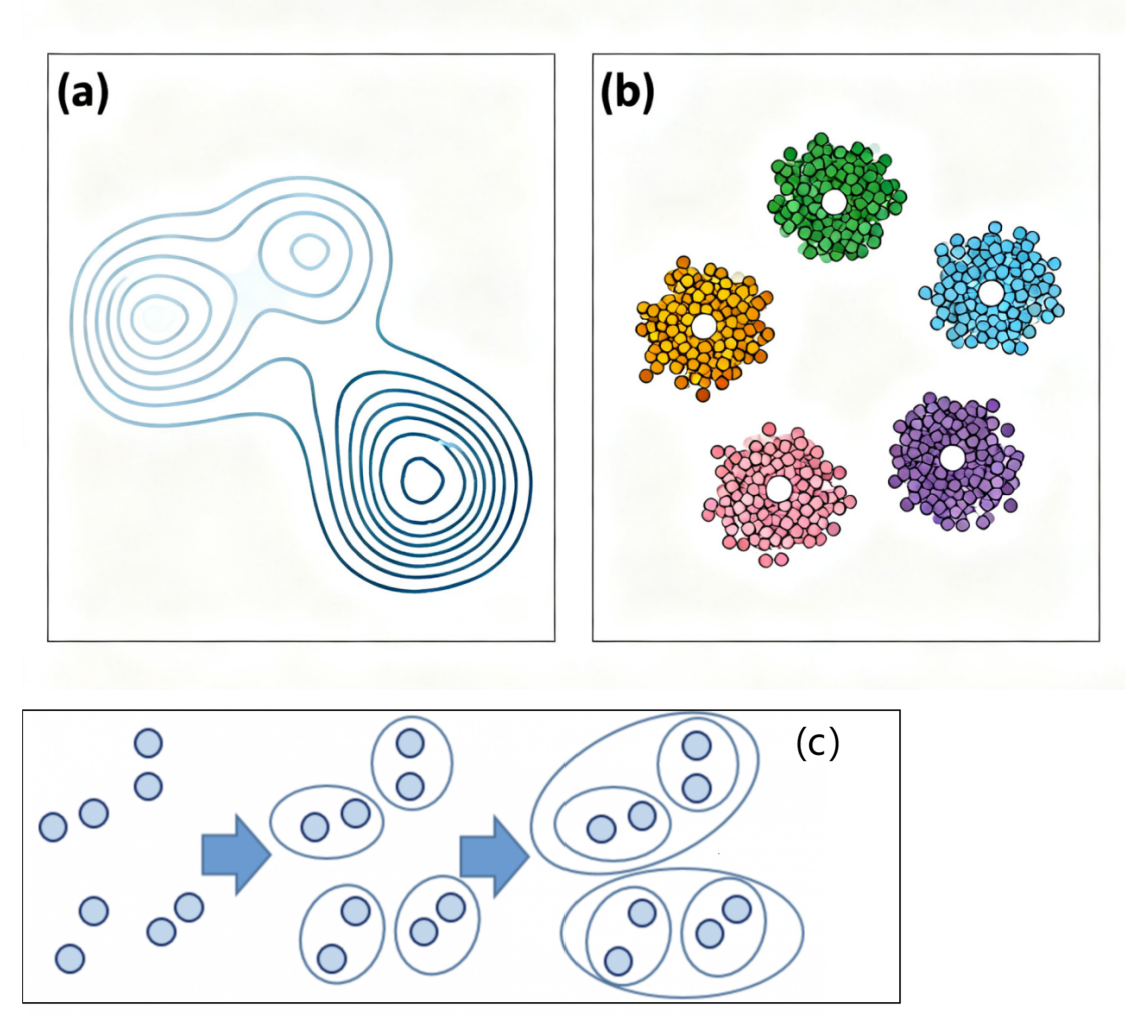
\includegraphics[width=0.8\textwidth]{figure/2_3_聚类方法对比.png}
\caption{不同类型的聚类方法示意图：(a)基于密度的聚类 (b)基于类中心的聚类 (c)层次聚类}
\end{figure}

K-means聚类算法是人工智能、机器学习、运筹学、统计学等诸多领域最常用的聚类算法之一。与max-cut、min-cut问题类似，K-means也是一个经典的随机算法的例子，其简单性和有效性使其在实践中得到了广泛应用。

\subsection{问题定义与基础概念}

\subsubsection{K-means聚类问题}

\begin{definition}[k-means聚类]
    输入欧式空间中$n$个点的集合$X=\{x_1,x_2,....,x_n\}\in R^d$, 希望找到$k$个类中心点$C=\{c_1,...,c_k\}\in R^d$,使得将集合$X$中的点分配给最近的类中心点，分配代价
    $\phi_{X}(C)=\sum_{x\in X}\mathop{min}_{c\in C}\left\lVert c-x \right\rVert_2^2$最小。
\end{definition}
为了后续分析方便，我们引入一些记号：

\begin{definition}
对于任意点集$A$和中心点集合$C$，定义分配代价$\phi_A(C) = \sum_{x \in A} \min_{c \in C} |c - x|_2^2$。
\end{definition}

\begin{remark}
如果将分配代价中的平方距离改为普通欧氏距离，即$\phi_A(C) = \sum_{x \in A} \min_{c \in C} ||c - x||_2$，则对应的聚类问题为k-median问题。
\end{remark}


\begin{definition}
    记$A_1,...,A_k$为最优解$C_{opt}$导出的类。其中$A_i=\{x\in X|c_i=\mathop{argmin}_{c\in C}\left\lVert c-x \right\rVert_2^2\}$。
\end{definition}
\subsubsection{计算复杂度与近似算法}

对于 K-means 问题，只要聚类数 $k$ 和维度 $d$ 有一个不是常数，那么它就是 NP-hard 的。这意味着在多项式时间内找到精确最优解在计算上是不可行的（除非 P = NP）。因此，我们转向研究能在多项式时间内找到近似解的近似算法。

近似算法的目标是，在可接受的时间内，找到一个解，其目标函数值（如 K-means 中的 $\phi_X(C)$）与最优解的比值（即近似比）有可证明的上界。

\begin{definition}[$\rho$-近似算法]
对于一个最优化问题，如果一个算法 $ALG$ 对于任何输入实例 $I$，都能在多项式时间内输出一个可行解，且满足：
\begin{itemize}
    \item 对于\emph{最小化问题}，该解的成本 $ALG(I)$ 满足：
    \[
    \frac{\mathrm{ALG}(I)}{\mathrm{OPT}(I)} \leq \rho
    \]
    \item 对于\emph{最大化问题}，该解的价值 $ALG(I)$ 满足：
    \[
    \frac{\mathrm{OPT}(I)}{\mathrm{ALG}(I)} \leq \rho
    \]
\end{itemize}
其中 $\mathrm{OPT}(I)$ 是该实例最优解的成本（对于最小化问题）或价值（对于最大化问题），则称 $ALG$ 是一个 $\rho$-近似算法。$\rho \geq 1$ 被称为该算法的\emph{近似比}。
\end{definition}
在两种情况下，近似比 $\rho$ 都大于等于 1。$\rho$ 越接近 1，表示近似算法得到的解越接近最优解。当 $\rho = 1$ 时，算法总能找到最优解。
\begin{definition}[多项式时间近似方案]
如果对于任意给定的 $\epsilon > 0$，都存在一个算法 $A_\epsilon$，使得 $A_\epsilon$ 是 $(1+\epsilon)$-近似算法，并且其运行时间是输入规模的多项式（对于固定的 $\epsilon$），则称该问题存在一个多项式时间近似方案（Polynomial Time Approximation Scheme，简称PTAS）。
\end{definition}
PTAS 是强大的，因为我们可以通过选择更小的 $\epsilon$ 来获得任意接近最优的解。然而，运行时间可能随着 $\epsilon$ 的减小而急剧增长，例如 $O(n^{1/\epsilon})$。一种更严格的要求是完全多项式时间近似方案，其运行时间是 $1/\epsilon$ 和输入规模的多项式。
\paragraph*{K-means 的近似算法概览}K-means 的近似算法研究取得了丰富的成果，主要围绕不同参数（$k$, $d$）是常数还是变量展开：
\begin{itemize}
\item \textbf{$d$ 为常数时}：存在 PTAS。核心思想是，在低维空间中，可以利用空间划分技术（如网格、区域分解）来枚举候选解的空间。例如，\textbf{Local Search} 算法从一个初始解开始，反复尝试用一个新中心替换一个旧中心，如果代价降低则接受替换。可以证明，经过多项式次迭代后，该算法能收敛到一个局部最优解，且其代价与全局最优解的比值是一个常数。这一方向的开创性工作见于 \cite{matousek2000approximate}，该文首次给出了基于局部搜索的 PTAS。后续研究 \cite{kanungo2002local} 进一步分析和改进了局部搜索算法的性能。

\item \textbf{$k$ 为常数时}：同样存在 PTAS。此时，可以枚举所有可能的 $k$ 个中心的"候选集"。虽然所有数据点的组合太多，但可以证明，存在一个大小仅为 $n$ 的多项式的候选中心集合，从中选出的 $k$ 个中心能提供 $(1+\epsilon)$-近似。\textbf{Peeling} 算法是这类算法的代表，它通过迭代地找到并移除最大簇的近似中心来工作。这方面的理论基础由 \cite{jaiswal2012k} 建立，他们提出了基于随机采样的 PTAS。更早的工作 \cite{kumar2010linear} 也为此类算法提供了重要的思路。

\item \textbf{$k$ 和 $d$ 均非常数时}：这是最一般也最困难的情况。此时不存在 PTAS（除非 P = NP），研究焦点在于设计常数因子近似算法。\textbf{K-means++} 及其变种（如之后将要介绍的 Bicriteria 算法）是这方面的杰出代表，它们通过巧妙的概率采样来初始化中心点，以高概率保证常数近似比。K-means++ 算法由 \cite{arthur2006k} 提出，首次实现了 $O(\log k)$ 的期望近似比。后续工作 \cite{aggarwal2009analysis} 提出了双准则近似算法，将近似比改进到常数级别。近年来，\cite{aghazadeh2020fast} 等研究进一步优化了这些算法的运行时间。
\end{itemize}
\paragraph*{从理论到实践}

理论上的近似比保证了算法在最坏情况下的性能下限。在实践中，像 Lloyd 算法这样没有近似比保证的启发式算法，由于其简单性和在“典型”实例上的良好表现，依然被广泛使用。K-means++ 的成功在于它很好地结合了理论保证和实际效能：其初始化步骤提供了理论上的近似比，而后续的 Lloyd 迭代则负责在实际数据上进一步优化。

理解这些近似算法的理论基础，不仅能让我们在面临困难问题时知道有哪些工具可用，更重要的是，它指导我们如何设计新的算法，以及如何根据数据的具体特点（大小、维度、簇数）来选择合适的现有算法。

\subsubsection{重心的性质}

\begin{definition}[重心]
    给定欧氏空间$\mathbb{R}^d$中任意一个点集$S$，其重心定义为
    $\mu(S)=\frac{1}{|S|}\sum_{x\in S}x$。
    其中$|S|$为点集$S$中点的个数。
\end{definition}
\begin{theorem}[重心的最优性]
对于欧氏空间$\mathbb{R}^d$中的一个点集$S$，其重心到点集中所有点的距离平方和最小，即
    \[
    \mu(S)=\mathop{argmin}_{c\in R^d}\frac{1}{|S|}\sum_{x\in S}\left\lVert x-c \right\rVert_2^2\]
\end{theorem}
\begin{proof}
\begin{align*}
    \sum_{x\in S}\left\lVert x-c \right\rVert_2^2&=\sum_{x\in S}\left\lVert x-\mu(S) + \mu(S) -c \right\rVert_2^2\\
    &=\sum_{x\in S}(\left\lVert x-\mu(S) \right\rVert_2^2 + \left\lVert \mu(S)-c\right\rVert_2^2 + 2\langle x-\mu(S) , \mu(S)-c\rangle)\\
    &=\sum_{x\in S}\left\lVert x-\mu(S) \right\rVert_2^2+|S|\left\lVert \mu(S)-c \right\rVert_2^2
\end{align*}
要使得$\sum_{x\in S}\left\lVert x-c \right\rVert_2^2$最小，则$\mu(S)-c = 0$，即$c = \mu(S)$
\end{proof}
上面的证明可以引出下面的技术性引理，后续会经常用到。
\begin{lemma}\label{lmm:barycenter}
    给定欧氏空间$R^d$中任意一个点集$S$以及$p\in R^d$,
    我们有$$\sum_{x\in S}\left\lVert x-p \right\rVert_2^2=\sum_{x\in S}\left\lVert x-\mu(S) \right\rVert_2^2+|S|\left\lVert \mu(S)-p \right\rVert_2^2$$
\end{lemma}


\subsection{经典算法及其分析}
\subsubsection{Lloyd算法}
\begin{algorithm}[H]
\caption{Lloyd's Algorithm}
\begin{algorithmic}
\State 均匀随机选取$k$个点作为$C$的初始化
\While{算法未收敛}
\State 将$X$根据$C$中的$k$个类中心进行划分，得到$k$个类$H_1,\ldots,H_k$
\State 对每一个类$H_j$，更新类中心$c_j \leftarrow \mu(H_j)$
\EndWhile
\end{algorithmic}
\end{algorithm}
Lloyd算法实现简单，时间复杂度为$O(nkd)$，但可能会陷入局部最优解，并且没有对近似比的保证。如果初始化的点选取不当，算法性能可能很差。例如考虑对一个长宽比非常大的矩形的四个顶点做二分类，如初始化将每条长划分成一类，上述算法将输出这个划分。显然，这和最优划分相距甚远。
\begin{figure}[htbp]
\centering
\begin{tikzpicture}[scale=0.7]

% 初始化 (左上)
\begin{scope}[xshift=-3cm, yshift=3cm]
    \draw[->] (-1.5,0) -- (1.5,0);
    \draw[->] (0,-1.5) -- (0,1.5);
    
    % 随机数据点
    \foreach \x/\y in {-1/1, -0.5/0.8, 0.3/1.2, 1/0.9, -0.8/-0.5, 0.2/-1, 0.9/-0.8, -1.2/0.3} 
        \fill[gray] (\x,\y) circle (2pt); % 增大到2pt
    
    % 初始中心 - 改为圆形
    \fill[black] (-1,0.5) circle (3pt); % 圆形，比数据点大
    \fill[black] (0.5,0.5) circle (3pt);
    \fill[black] (0,-0.5) circle (3pt);
    
    \node[below, align=center] at (0,-1.8) {1. 初始化\\随机选择中心};
\end{scope}

% 分配点 (右上)
\begin{scope}[xshift=3cm, yshift=3cm]
    \draw[->] (-1.5,0) -- (1.5,0);
    \draw[->] (0,-1.5) -- (0,1.5);
    
    % 分配后的点 - 增大点的大小
    \foreach \x/\y in {-1/1, -0.5/0.8, -1.2/0.3} 
        \fill[red] (\x,\y) circle (2.5pt); % 增大到2.5pt
    \foreach \x/\y in {0.3/1.2, 1/0.9} 
        \fill[blue] (\x,\y) circle (2.5pt);
    \foreach \x/\y in {-0.8/-0.5, 0.2/-1, 0.9/-0.8} 
        \fill[green] (\x,\y) circle (2.5pt);
    
    % 中心点 - 改为圆形并增大
    \fill[black] (-1,0.5) circle (4pt); % 增大到4pt
    \fill[black] (0.5,0.5) circle (4pt);
    \fill[black] (0,-0.5) circle (4pt);
    
    % 连接线
    \draw[red, dashed] (-1,1) -- (-1,0.5);
    \draw[blue, dashed] (1,0.9) -- (0.5,0.5);
    \draw[green, dashed] (0.9,-0.8) -- (0,-0.5);
    
    \node[below, align=center] at (0,-1.8) {2. 分配点\\到最近中心};
\end{scope}

% 更新中心 (左下)
\begin{scope}[xshift=-3cm, yshift=-3cm]
    \draw[->] (-1.5,0) -- (1.5,0);
    \draw[->] (0,-1.5) -- (0,1.5);
    
    % 数据点 - 保持较大的点
    \foreach \x/\y in {-1/1, -0.5/0.8, -1.2/0.3} 
        \fill[red] (\x,\y) circle (2.5pt);
    \foreach \x/\y in {0.3/1.2, 1/0.9} 
        \fill[blue] (\x,\y) circle (2.5pt);
    \foreach \x/\y in {-0.8/-0.5, 0.2/-1, 0.9/-0.8} 
        \fill[green] (\x,\y) circle (2.5pt);
    
    % 新中心位置 - 改为彩色圆形
    \fill[red] (-0.9,0.7) circle (4pt);
    \fill[blue] (0.65,1.05) circle (4pt);
    \fill[green] (0.1,-0.77) circle (4pt);
    
    % 旧中心位置（灰色，显示移动）
    \fill[gray!50] (-1,0.5) circle (3pt);
    \fill[gray!50] (0.5,0.5) circle (3pt);
    \fill[gray!50] (0,-0.5) circle (3pt);
    
    % 移动箭头
    \draw[->, thick, black] (-1,0.5) -- (-0.9,0.7);
    \draw[->, thick, black] (0.5,0.5) -- (0.65,1.05);
    \draw[->, thick, black] (0,-0.5) -- (0.1,-0.77);
    
    \node[below, align=center] at (0,-1.8) {3. 更新中心\\重新计算质心};
\end{scope}

% 最终结果 (右下)
\begin{scope}[xshift=3cm, yshift=-3cm]
    \draw[->] (-1.5,0) -- (1.5,0);
    \draw[->] (0,-1.5) -- (0,1.5);
    
    % 最终聚类 - 保持较大的点
    \foreach \x/\y in {-1/1, -0.5/0.8, -1.2/0.3, -0.8/0.9} 
        \fill[red] (\x,\y) circle (2.5pt);
    \foreach \x/\y in {0.3/1.2, 1/0.9, 0.8/1.1} 
        \fill[blue] (\x,\y) circle (2.5pt);
    \foreach \x/\y in {-0.8/-0.5, 0.2/-1, 0.9/-0.8, 0.1/-0.9} 
        \fill[green] (\x,\y) circle (2.5pt);
    
    % 最终中心 - 改为彩色圆形
    \fill[red] (-0.88,0.75) circle (4pt);
    \fill[blue] (0.7,1.07) circle (4pt);
    \fill[green] (0.1,-0.8) circle (4pt);
    
   
    
    \node[below, align=center] at (0,-1.8) {4. 最终结果\\收敛状态};
\end{scope}

\end{tikzpicture}
\caption{Lloyd算法迭代过程示意图}
\end{figure}
\subsubsection{K-means++算法}

\begin{algorithm}[H]
\caption{K-means++ \cite{arthur2006k}}
\begin{algorithmic}
\State 初始化$C \leftarrow {c_1}$，$c_1$为$X$中随机选取的点
\For{$j = 2,3,\ldots,k$}
\State $p(x) \leftarrow \dfrac{\min_{1 \leq \ell \leq j-1} |x - c_\ell|_2^2}{\phi_X(C)}$
\State 以概率$p(x)$选取$X$中点$c_j$放入$C$中
\EndFor
\State 以上面得到的$C$作为Lloyd's Algorithm类中心的初始化，运行Lloyd's Algorithm
\end{algorithmic}
\end{algorithm}
该算法由\cite{Aggarwal2009Adaptive}提出，其核心思想是以更高概率选取距离现有中心较远的点。为什么不直接使用贪心的思想？其实我们希望选出离最优解中心接近的点，这样的点往往并不是距离现有中心最远的点。直觉上最优解中心周围的点会比较稠密，这样选取到最优解中心周围点的概率和很大，于是会以更高概率取得离最优解中心接近的点。该算法的近似比期望为$8\log(k)$，时间复杂度为$O(nkd)$.

\phantomsection
\subsubsection{双准则近似算法}
下面介绍的算法是上面算法的一个变种, 很多时候我们并不确定需要将数据聚成多少类,如果我们允许返回多于$k$个类，那么可以将cost显著降低，对于原本$k$聚类的算法能讲近似比改进到常数。
\begin{algorithm}[H]
\caption{Bicriteria Approximation for K-means}
\begin{algorithmic}
\State 初始化$C \leftarrow {c_1}$，$c_1$为$X$中随机选取的点
\For{$j = 2,3,\ldots,k,\ldots,16(k+\sqrt{k})$}
\State $p(x) \leftarrow \dfrac{\min_{1 \leq \ell \leq j-1} |x - c_\ell|_2^2}{\phi_X(C)}$
\State 以概率$p(x)$选取$X$中点$c_j$放入$C$中
\EndFor
\State 返回$C$
\end{algorithmic}
\end{algorithm}

根据下面的定理，该算法将返回大于$k$个类，但是会将近似比变成常数。
如果我们记对于$k$个类的最优解为$C_{opt}$，那么
$\phi_X(C)\leq 20\phi_X(C_{opt})$ 以至少常数概率(大概3\%)成立。
\begin{theorem}
如果运行K-means++ Sampling $t = 16(k+\sqrt{k}) = \Theta(k)$步，令得到的集合为S，则$\phi_X(S)\leq 20\phi_X(C_{opt})$以常数概率成立
\end{theorem}
\subsubsection{理论分析}
为了证明上述定理，我们引入一些关键定义和引理。
\paragraph*{基础定义}

定义算法运行到第$i$步时的类中心集合为$S_i$，初始集合$S_0 = \emptyset$。在第$i$步，我们将最优解导出的类${A_1,\ldots,A_k}$分为两种集合：

\begin{itemize}
\item $\text{Good}i = {A_j \mid \phi{A_j}(S_{i-1}) \leq 10\phi_{A_j}(C_{opt})}$
\item $\text{Bad}_i = {A_1,\ldots,A_k} \setminus \text{Good}_i$
\end{itemize}

如果存在某个时刻$j$，$\text{Bad}_j = \emptyset$，说明我们已经得到10近似比的解。
\paragraph*{关键引理}

\begin{lemma}
假设在第$i$步有两种事件：
\begin{itemize}
\item $A = {\phi_X(S_{i-1}) \leq 20\phi_X(C_{opt})}$
\item $B = {c_i \in \text{Bad}_i}$（$c_i$为第$i$步采到的点）
\end{itemize}
那么$P[B \mid A^c] \geq \frac{1}{2}$。
\end{lemma}
该引理说明，如果当前解不满足要求（代价大于20倍最优解），那么下一步采到坏类中的点的概率将大于50\%。进一步，如果采样得到的点位于坏类，那么坏类的代价将大概率降低，从而很可能将坏类转变为好类
\begin{proof}
集合$\mathit X$对于类中心$\mathit S_{\mathit i-1}$的代价可以分为两部分,集合$\mathit Good_{i}$对于类中心的代价和集合$\mathit Bad_{i}$对于类中心的代价，即
\[
    \phi_X(S_{i-1}) = \sum_{A_j \in Good_i} \phi_{A_j}(S_{i-1}) + \sum_{A_j \in Bad_i} \phi_{A_j}(S_{i-1}).
    \]
由Good集合的定义知：\( \phi_{A_j}(S_{i-1}) \leq 10 \phi_{A_j}(C_{opt}) \),
于是有：
\[
    \phi_X(S_{i-1}) \leq \sum_{A_j \in Good_i} 10 \phi_{A_j}(C_{opt}) + \sum_{A_j \in Bad_i} \phi_{A_j}(S_{i-1}).
    \]
因为\( \phi_X(C_{opt}) = \sum_{A_j} \phi_{A_j}(C_{opt}) \geq \sum_{A_j \in Good_i} \phi_{A_j}(C_{opt})\)\\
故\[
    \phi_X(S_{i-1}) \leq 10 \phi_X(C_{opt}) + \sum_{A_j \in Bad_i} \phi_{A_j}(S_{i-1}).
    \]
由于$A^c$意味着\( \phi_X(S_{i-1}) > 20 \phi_X(C_{opt}) \)，因此
 \[
    \sum_{A_j \in Bad_i} \phi_{A_j}(S_{i-1}) \geq  10 \phi_X(C_{opt}).
    \]
算法运行到第i步时，算法在该步选择的点$\mathit c_{\mathit i}\in\mathit Bad_{i}$的概率等于:
\begin{align*}
\frac{\sum_{A_j \in Bad_i} \phi_{A_j}(S_{i-1})}{\phi_X(S_{i-1})} 
&= \frac{\sum_{A_j \in Bad_i} \phi_{A_j}(S_{i-1})}{\sum_{A_j \in Bad_i} \phi_{A_j}(S_{i-1}) + \sum_{A_j \in Good_i} \phi_{A_j}(S_{i-1})} \\
&= \frac{1}{1 + \frac{\sum_{A_j \in Good_i} \phi_{A_j}(S_{i-1})}{\sum_{A_j \in Bad_i} \phi_{A_j}(S_{i-1})}} \\
&\geq 50\%
\end{align*}
\end{proof}

\begin{lemma}
    $\forall A_j\in Bad_i$, 定义其平均半径$r=\sqrt{\frac{1}{|A_j|}\phi_{A_j}(C_{opt})}$.同时定义$d=\mathop{\min}_{y\in S_{i-1}}\left\lVert y-\mu(A_j) \right\rVert$。那么我们有$d\geq 3r$.
\end{lemma}

\begin{proof}
    对于任意一个$A_j\in Bad_i$,根据定义我们有 $d=\min _{y\in S_{i-1}} \|y-\mu(A_{j})\|$，并且
\begin{align*}
    10\cdot \phi_{A_j}(C_{opt})&<\phi_{A_j}(S_{i-1})\\
    &=\sum_{x\in A_j}\min_{y\in S_{i-1}}\left\lVert x-y\right\rVert_2^2\\
    &\leq \sum_{x\in A_j}\left\lVert x-y_0\right\rVert_2^2\\
    &=\Phi_{A_{j}}(C_{opt})+|A_{j}|\cdot d^{2}
\end{align*}
整理上式即可得到$d\ge 3r$。
\end{proof}




\begin{lemma}
    定义核心点集 $B_{A_{j}}(\alpha)=\{x\in A_{j}|\|x-\mu(A_{j})\|\le \alpha\cdot r\}$，其中$0\le \alpha\le 3$。$\forall b\in B_{A_{j}}(\alpha)$, $\Phi_{A_{j}}(S_{i-1}\cup \{b\}) \le 10\cdot \Phi_{A_{j}}(C_{opt}).$
\end{lemma}
该引理说明，只要我们采到一个坏类的核心区域的点集，该类的代价就会小于10倍的最优解，从而变成好类
\begin{proof}
    可以用$b$来替代 $\mu(A_{j})$，可以得到\[\Phi_{A_{j}}(S_{i-1}\cup \{b\})\le (1+\alpha^{2})\cdot\Phi_{A_{j}}(C_{opt})\le 10\cdot \Phi_{A_{j}}(C_{opt}) \]
    这里利用到了引理\ref{lmm:barycenter}
\end{proof}

\begin{lemma}
    $|B_{A_{j}(\alpha)}|\ge (1-\frac{1}{\alpha^{2}})|A_{j}|$
\end{lemma}

\begin{proof}
    \begin{align*}
        \Phi_{A_{j}}(C_{opt})& \ge \sum _{x\in A_{j}\setminus B(\alpha)}\|x-\mu(A_{j})\|^{2}\\
        &\ge(|A_{j}-|B_{A_{j}}|)\cdot(\alpha r)^{2}\\
        &= (1-\frac{|B_{A_{j}}|}{|A_{j}|})\cdot\alpha^{2}\cdot \Phi_{A_{j}}(C_{opt}).
    \end{align*} 
整理上式即可。
\end{proof}

\begin{lemma}
    假设 $x$ 为通过 kmeans++ 采到的点，则 $\Pr[x\in B_{A_{j}}(\alpha)|A_{j}\in Bad_{i},x\in A_{j}]=\frac{\Phi_{B_{A_{j}}}(S_{i-1})}{\Phi_{A_{j}}(S_{i-1})}\ge \frac{(3-\alpha)^2}{10}\cdot (1-\frac{1}{\alpha^{2}})$
    
\end{lemma}
该引理说明，如果我们采到坏类中的点，那么大概率会采到坏类核心区域的点
\begin{proof}由三角不等式，
    $$\Phi_{B_{A_{j}}}(S_{i-1})\ge |B_{A_{j}}|\cdot (d-\alpha r )^{2}$$ 
    除此之外，
    \begin{align*}
        \Phi_{A_{j}}(S_{i-1}) &\le \sum_{x\in A_{j}}\|x-y_{0}\|^{2} \\
        &\le \sum_{x\in A_{j}}\|x-\mu(A_{j})\|^{2}+|A_{j}|\cdot\|\mu(A_{j})-y_{0}\|^{2}\\
        &\le \Phi_{A_{j}}(C_{opt})+|A_{j}|\cdot\\
        &\le |A_{j}|(r^{2}+d^{2}).
    \end{align*}
因此\begin{align*}
    \Pr[x\in B_{A_{j}}(\alpha)|A_{j}\in Bad_{i},x\in A_{j}]&\ge \frac{|B_{A_{j}}|\cdot(d-\alpha r)^{2}}{|A_{j}|\cdot (r^{2}+d^{2})}\\
    &\ge \frac{(d-\alpha r)^{2}}{r^{2}+d^{2}}\cdot(1-\frac{1}{\alpha^{2}})\\
    &\ge (1 - \frac{1}{\alpha^{2}})\cdot \frac{(3-\alpha)^{2}}{10}
\end{align*}
\end{proof}

通过上述引理，$S_{i}=S_{i-1}\cup \{x\}$，令 $\alpha\approx 1.44225$，则$\Pr[\Phi_{A_{j}}\le 10\Phi_{A_{j}}(C_{opt})|x\in A_{j}, A_{j}\in Bad_{i}]\ge 0.126$. (通过数值计算得到)。

回到$\beta$ Giteria approximation 的分析，通过引理2.4和上述不等式， $\Pr[|Bad_{i-1}|<|Bad_{i}|\mid|A^{c}]\ge 0.063$。这说明，我们每采一个点，坏类的数量至少减一的概率大于0.063。\\
定义一个随机变量序列 $q_{i}$, $i=1,2,\cdots$ \[q_{i}=1, \text{if }\; |Bad_{i+1}|=|Bad_{i}|\] \[q_{i}=0, \text{if }\; |Bad_{i+1}| < |Bad_{i}|\]
因此，$\Pr[q_{i}=0|q_{1},\cdots,q_{i-1}]=0.063\triangleq p$ 并且 $E[q_{i}|q_{1},\cdots,q_{i-1}]=1-p$. 令 $J_{i}=\sum_{1\le j\le i}(q_{i}-(1-q))$, 所以$J_{i+1}-J_{i}\le 1$。我们可以验证 $J_{i}$ 序列是一个上鞅 $$E[J_{i}|J_{1},\cdots, J_{i-1}]=E[J_{i-1}+q_{i}-(1-p)|J_{1},\cdots, J_{i-1}]\le J_{i-1}$$
因此通过 Azuma 不等式，\[\Pr[J_{t}\ge J_{1}+\delta]\le e^{-\frac{\delta}{2t}}\]
设置 \[t=\frac{k+\sqrt{k}}{p}<16(k+\sqrt{k}), \delta=\sqrt{k}\] 我们能得到
\[\Pr[\sum_{i=1}^{t}(1-q_{i})\ge k]\ge 0.03\] 
这说明至少以0.03的概率，$t$ 时刻没有 Bad cluster。 更一般地，设置 $t=O(\frac{k}{\epsilon}\log (\frac{1}{\epsilon}))$ 即允许输出的类更多的时候，我们能得到 $(4+\epsilon)$的近似比，比之前的 $q\cdot \log(k)$ 更好，当 $k$ 很大的时候。
\subsection{双层近似的分析}
上面的算法虽然有更强的近似比保证，但是它返回的类中心多于k个。如果我们只想得到k个类中心，不允许多余，怎么办呢？一个显然的想法是，我们在运行Bicriteria approximation for K-means算法后，对得到的中心再进行一次kmeans聚类，得到严格的k个类中心。那么随之而来的一个问题是，这种双层近似的方法有怎样的性能保证呢？下面我们来研究这个问题。

\begin{figure}[htbp]
\centering
\begin{tikzpicture}[node distance=2cm, auto]

% 节点定义
\node (input) [draw, rectangle, fill=blue!10, minimum width=3cm, align=center] 
    {输入：点集 $X \subseteq \mathbb{R}^d$\\数据点云};
    
\node (algA) [draw, rectangle, fill=green!10, minimum width=3cm, align=center, below of=input] 
    {算法A：双准则近似\\输出：$|S| = \lambda k$ 个中心\\保证：$\phi_X(S) \leq c \cdot \phi_X(C_{opt})$};

\node (algB) [draw, rectangle, fill=orange!10, minimum width=3cm, align=center, below of=algA] 
    {算法B：K-means聚类\\输入：中心点集合 $S$\\输出：$|O| = k$ 个中心\\保证：$\phi_S(O) \leq \beta \cdot \phi_S(O_{opt})$};

\node (output) [draw, rectangle, fill=red!10, minimum width=3cm, align=center, below of=algB] 
    {最终输出：$k$ 个类中心\\联合保证：$\phi_X(O) \leq [2c + (2c+2)\cdot 2\beta] \cdot \phi_X(C_{opt})$};

% 连接箭头
\draw[->, thick] (input) -- node[right] {原始数据} (algA);
\draw[->, thick] (algA) -- node[right] {$\lambda k$ 个中心} (algB);
\draw[->, thick] (algB) -- node[right] {最终 $k$ 个中心} (output);



\end{tikzpicture}
\caption{两种聚类方法的结合}
\end{figure}
假设我们有欧式空间上的一个点集X，我们首先在X上运行算法A，得到$\lambda k$个类中心S，然后在S上运行算法B，得到k个类中心，其中算法A和B的近似比分别为c和$\beta$，即：
\begin{align*}
    |{S}|=\lambda k, \phi_X(S)\leq c \phi_X(C_{opt})\\
    |O|=k, \phi_S(O)\leq \beta\phi_S(O_{opt})
\end{align*}
对于X中的一个点x,假设在S集合中离他最近的点为S(x)，在O中离他最近的点为O(x),并且在O中，离S(x)最近的点为O(S(x))\\
那么有
\[
\left\lVert x-O(x)\right\rVert^2 \leq \left\lVert x-O(S(x))\right\rVert^2 \leq 2\left\lVert x-S(x)\right\rVert^2 + 2\left\lVert S(x)-O(S(x))\right\rVert^2
\]
两边求和有$\phi_X(O) \leq 2\phi_X(S) + 2 \phi_S(O) = 2c\phi_X(C_{opt})+2\beta\phi_S(O_{opt})$\\
$C_{opt}$是S的一个可行解，那么有$\phi_S(O_{opt})\leq\phi_S(C_{opt})$\\
假设在$C_{opt}$中，离S(x)最近的点为C(S(x)),离x最近的点为C(x),那么有
\[
\left\lVert S(x)-C(S(x))\right\rVert^2 \leq \left\lVert S(x)-C(x)\right\rVert^2 \leq 2\left\lVert S(x)-x\right\rVert^2 + 2\left\lVert x-C(x)\right\rVert^2
\]
两边求和有$\phi_S(C_{opt}) \leq 2\phi_X(S) + 2 \phi_X(C_{opt}) = (2c+2)\phi_X(C_{opt})$\\
综合上面三个不等式，我们有
\[
\phi_X(O) \leq (2c+(2c+2)2\beta)\phi_X(C_{opt})
\]
这也是直接使用这两个近似算法的联合近似比

\section{Karger算法}
\subsection{图上的最小割}

给定一个无向图 \( G = (V, E) \) 和边上的容量 \( c: E \to \mathbb{R}_{\geq 0} \)。一个割 \( (S, T) \) 是顶点集 \( V \) 的一个划分，其中 \( S \cup T = V \) 且 \( S \cap T = \emptyset \)。割的容量定义为：
\[
c(S, T) = \sum_{u \in S, v \in T} c(u, v)
\]
其中，如果 \( (u, v) \notin E \)，则约定 \( c(u, v) = 0 \)。

我们的问题是：找到一个割 \( (S, T) \)，使得 \( c(S, T) \) 的值最小。

\subsubsection{Karger 的随机收缩算法}

Karger 算法\cite{karger1993n2}是一种随机化的方法，用于近似求解最小割问题。其核心思想是通过重复随机选择并收缩图中的边，直到图中只剩下两个顶点为止。具体步骤如下：

\begin{enumerate}
    \item 当图中顶点的数量超过 2 个时，执行以下操作：
    \begin{enumerate}
        \item 从边集 \( E \) 中按照均匀分布随机选择一条边 \( (u, v) \)。
        \item 将顶点 \( u \) 和 \( v \) 合并成一个新的顶点 \( S_{u,v} \)，并移除边 \( (u, v) \)。
        \item 对于每条原来与 \( u \) 或 \( v \) 相连的边，例如 \( (x, u) \) 或 \( (x, v) \)，将其替换为一条新的边 \( (x, S_{u,v}) \)，并赋以容量$\c(x,u)+c(x,v)$。
      %  \item 如果在合并过程中产生了自环（即边 \( (w, w) \)），则移除所有自环。
    \end{enumerate}
    \item 对得到的图重复上述步骤，直到图中只剩下 2 个顶点$S_X, S_{\bar X}$为止。
    \item 最后，返回由这两个顶点定义的割 \( (X, \bar X) \) 及其容量。
\end{enumerate}

需要注意的是，每次运行该算法时，返回的割是随机的。

\subsubsection{成功的概率}

假设图 \( G \) 的最小割的大小为 \( k \)，即 \( \min_{S,T} c(S, T) = k \)。我们希望分析 Karger 算法能够成功找到这个最小割的概率。

首先， 图 \( G \) 中至少有 \( k \) 条边横跨最小割 \( (S^*, T^*) \)。
    因为 \( G \) 是一个无向图，每个顶点的度数必须至少为 \( k \)。如果某个顶点的度数小于 \( k \)，那么以这个顶点为一侧的割的容量将小于 \( k \)，这与 \( k \) 是最小割大小的假设矛盾。
因此，图 \( G \) 的总边数满足 \( |E| \geq \frac{k n}{2} \)，其中 \( n = |V| \) 是图中顶点的总数。


现在，我们分析算法在第一次收缩时的行为：
 此时，图中的边总数为 \( |E| \geq \frac{k n}{2} \)。
m 横跨最小割 \( (S^*, T^*) \) 的边数恰好为 \( k \)。
随机选择一条边时，选择一条横跨最小割的边的概率为：
    \[
    \Pr[\text{选择的边横跨 } (S^*, T^*)] = \frac{k}{|E|} \leq \frac{k}{\frac{k n}{2}} = \frac{2}{n}
    \]
  因此，选择一条不横跨最小割的边的概率至少为：
    \[
    1 - \frac{2}{n}
    \]

接下来，考虑第二次收缩。此时，图中的顶点数变为 \( n-1 \)。由于每个顶点的度数仍然至少为 \( k \)，边数虽然减少，但总边数仍然满足 \( |E'| \geq \frac{k (n-1)}{2} \)。类似地，选择一条不横跨最小割的边的概率至少为：
\[
1 - \frac{2}{n-1}
\]

以此类推，在算法的每次迭代中，顶点数逐渐减少。总体而言，算法成功找到最小割的概率（即在整个过程中从未选择横跨最小割的边）可以表示为：
\[
\prod_{i=3}^{n} \left(1 - \frac{2}{i}\right)
\]

我们计算这个乘积：
\[
\prod_{i=3}^{n} \left(1 - \frac{2}{i}\right) = \frac{(n-2)(n-3) \cdots 3 \cdot 2 \cdot 1}{n (n-1) (n-2) (n-3) \cdots 3} = \frac{(n-2)!}{n! / (2 \cdot 1)} = \frac{(n-2)!}{\frac{n (n-1) (n-2)!}{2}} = \frac{2}{n (n-1)}
\]

因此，Karger 算法单次运行成功找到最小割的概率至少为：
\[
\frac{2}{n (n-1)}
\]

这表明成功概率的量级为 \( \Omega\left(\frac{1}{n^2}\right) \)。

\subsubsection{改进成功概率}

单次运行 Karger 算法找到最小割的概率较低，仅为 \( \Omega(1/n^2) \)。然而，我们可以通过多次独立运行该算法并从所有运行结果中选择容量最小的割来显著提高成功概率。

具体来说： 假设我们运行算法 \( n^2 \) 次。
 每次运行失败（即未找到最小割）的概率为：
    \[
    1 - \frac{2}{n (n-1)}
    \]
 \( n^2 \) 次运行全部失败的概率为：
    \[
    \left(1 - \frac{2}{n (n-1)}\right)^{n^2}
    \]
 因为 \( \frac{2}{n (n-1)} \approx \frac{2}{n^2} \)（当 \( n \) 较大时），我们可以近似计算：
    \[
    \left(1 - \frac{2}{n (n-1)}\right)^{n^2} \leq \left(1 - \frac{1}{n^2}\right)^{n^2}
    \]
 根据不等式 \( 1 - x \leq e^{-x} \)，我们有：
    \[
    \left(1 - \frac{1}{n^2}\right)^{n^2} \leq e^{-\frac{n^2}{n^2}} = e^{-1} \approx 0.3679
    \]
   因此，至少有一次运行成功的概率为：
    \[
    1 - \left(1 - \frac{2}{n (n-1)}\right)^{n^2} \geq 1 - e^{-1} \approx 0.6321
    \]


这意味着，通过运行 \( n^2 \) 次 Karger 算法，我们以超过 \( 63\% \) 的概率能够找到最小割。通过运行 \( O(n^2) \) 次，成功概率可以提升到一个常数级别。每次运行算法要进行$n-1$次边收缩,每次边收缩要用时$O(n)$,总的算法复杂度为$O(n^4)$. 相当低效.

\subsection{改进的Karger-Stein算法}

在上一节中，我们分析了Karger-Stein算法的基本版本。现在，我们提出一个改进版本，通过更细致的递归调用策略来进一步提高效率。

\subsubsection{算法描述}

改进的Karger-Stein算法如下：

\begin{enumerate}
    \item 如果图$G$的顶点数$|V| \leq 6$，则使用暴力枚举法找到最小割
    \item 否则：
    \begin{enumerate}
        \item 设$t = \lceil 1 + |V|/\sqrt{2} \rceil$
        \item 构造两个图$G_1$和$G_2$，每个都是通过将$G$收缩到$t$个顶点得到的
        \item 递归计算$G_1$和$G_2$的最小割
        \item 返回两个结果中较小的那个
    \end{enumerate}
\end{enumerate}

\subsubsection{运行时间分析}

该算法的运行时间由以下递归关系给出：

\begin{equation*}
    T(n) = 2T\left(\left\lceil 1 + \frac{n}{\sqrt{2}} \right\rceil\right) + O(n^2)
\end{equation*}

我们可以使用主定理来分析这个递归关系。设收缩到$t$个顶点需要$O(n^2)$时间。

\begin{theorem}
改进的Karger-Stein算法的运行时间为$O(n^2 \log n)$。
\end{theorem}

\begin{proof}
展开递归树：
\begin{itemize}
    \item 第一层：$2$次调用(生成两个子问题,分别关于$G_1$和$G_2$)，规模为$\approx n/\sqrt{2}$
    \item 第二层：$4$次调用($G_i$各自又需构造两个图)，规模为$\approx n/2$
    \item 第三层：$8$次调用，规模为$\approx n/(2\sqrt{2})$
    \item ...
    \item 第$k$层：$2^k$次调用，规模为$\approx n/((\sqrt{2})^k)$
\end{itemize}

递归在$n/((\sqrt{2})^k) \leq 6$时停止，解得$k \approx 2 \log n$。

每层的总工作量为$O(n^2)$，因为：
\begin{equation*}
    \text{第}k\text{层工作量} = 2^k \cdot O\left(\left(\frac{n}{(\sqrt{2})^k}\right)^2\right) = O(n^2)
\end{equation*}

总共有$O(\log n)$层，因此总运行时间为$O(n^2 \log n)$。
\end{proof}

\subsubsection{成功概率分析}

首先是前$n-t$次收缩后保留最小割,然后是两个结果有至少一次成功,得到成功概率的递归关系为：

\begin{equation*}
    P(n) \geq \frac{1}{2}\left(1 - \left(1 -  P\left(\left\lceil 1 + \frac{n}{\sqrt{2}} \right\rceil\right)\right)^2\right)
\end{equation*}

\begin{theorem}
改进的Karger-Stein算法找到最小割的成功概率为$\Omega\left(\frac{1}{\log n}\right)$。
\end{theorem}

\begin{proof}
我们通过归纳法证明$P(n) \geq \frac{1}{c \log n}$，其中$c$是适当选择的常数。

基例：对于小的$n$，可以直接计算。

归纳步骤：假设对于所有$m < n$成立，则：

\begin{align*}
P(n) &\geq \frac{1}{2} \cdot\left(1 - \left(1 -  \frac{1}{c \log (n/\sqrt{2})}\right)^2\right) \\
%&= 1 - \left(1 - \frac{1}{2c (\log n - 0.5)}\right)^2 \\
&\approx \frac{1}{c (\log n - 0.5)} \quad \text{($a^2-b^2=(a+b)(a-b)$)} \\
&\geq \frac{1}{c \log n} \quad \text{(当$c$足够大)}
\end{align*}

因此，通过选择足够大的$c$，可以满足归纳假设。
\end{proof}

\subsubsection{进一步改进}

通过运行算法$O(\log n)$次并取最佳结果，我们可以将成功概率提高到常数级别，同时保持$O(n^2 \log^2 n)$的总运行时间。

\begin{corollary}
存在一个$O(n^2 \log^2 n)$时间的随机算法，能以高常数概率找到图的最小割。
\end{corollary}
\printbibliography[heading=subbibliography, title={本章参考文献}]
\addcontentsline{toc}{section}{参考文献} % 手动添加到目录
\end{refsection}

\begin{refsection}
\chapter{降维}
\section{主成分分析}
对于高维数据集，数据经常是非常稀疏的，一个合理的操作是将这些高维数据降为低纬数据。主流降维方法的主要的有三种：主成分分析、随机投影、特征选取. 深度学习方法还包括流形学习和编码器.


%#############################################################
%#############################################################
%#############################################################
%#############################################################

%\section{PCA: principle component analysis}

从几何的角度来说，对于集合 $P=\{p_{1},\cdots, p_{n}\}\subset R^{d}$，我们期望找到一个 $k$ ($k\ll d$)维的仿射子空间$E$，
\begin{equation*}
    min\sum_{i=1}^{n} \|p_{i}-\pi(p_{i})\|_{2}^{2}
\end{equation*}
其中 $\pi$ 是 $R^d$ 到 $E$的投影。%当然，此处的目标函数也可以替换为其他的度量。

从线性代数的角度讲，对于矩阵 $A\in R^{n\times d}$ 找到一个秩为 $k$的矩阵 $A_{k}$ 使得 $\|A-A_{k}\|_{F}$ 最小。其中 $\|X\|_{F}=\sqrt{\sum_{i,j}X_{ij}^{2}}$。 

当$k=0$，我们要寻找的是一个点，由定义可知就是$P$的重心$\nu(P)$。


\begin{definition}
    \begin{itemize}
    \item \textbf{重心（Centroid）}：点集 $\{P_i\}$ 的重心 $C$ 定义为所有点的平均位置：
    \[
    C = \frac{1}{N} \sum_{i=1}^{N} P_i
    \]
    \item \textbf{仿射子空间（Affine Subspace）}：一个 $k$ 维仿射子空间 $S$ 可以表示为 $S = v_0 + V$，其中 $V$ 是一个过原点的 $k$ 维向量子空间，而 $v_0$ 是一个平移向量。
\end{itemize}
\end{definition}


当$k>0$, $\nu(P)$ 应当还是在我们要寻找的子空间上：
% \begin{align*}
%    \sum_{i=1}^n\norm{p_i-\textbf{proj}_E(\nu(P))}_2^2&=\sum_{i=1}^n\norm{\textbf{proj}_E(p_i)-\proj{\nu(P)}}_2^2+\norm{\proj{p_i}-p_i}_2^2\\
%    &\leq\norm{\proj{p_i}-\proj{\nu(P)}}_2^2+\norm{p_i-\proj{p_i}}_2^2+\norm{\nu(P)-\proj{\nu(P)}}_2^2\\&=\norm{\p_i-\nu(P)}_2^2.
% \end{align*}
% 由重心的定义，可知不等号只能相等，即$\nu(P)\in E$.

\begin{proposition}
    给定一个点集 $\{P_1, P_2, \ldots, P_N\} \subset \mathbb{R}^d$，则到这些点距离平方和最小的 $k$ 维仿射子空间总是包含它们的重心。
\end{proposition}



\begin{proof}
    我们的目标是找到一个 $k$ 维仿射子空间 $S = v_0 + V$ 来最小化所有点到该子空间的距离平方和。这个距离平方和可以表示为：
\[
\mathcal{E}(v_0, V) = \sum_{i=1}^{N} \text{dist}(P_i, S)^2 = \sum_{i=1}^{N} \| \text{proj}_{V^\perp}(P_i - v_0) \|^2 \tag{1}
\]
其中，$\text{proj}_{V^\perp}(\cdot)$ 表示向向量子空间 $V$ 的正交补空间 $V^\perp$ 的正交投影。

为了简化问题，我们首先将点集平移，使得重心位于原点。
\begin{enumerate}
    \item \textbf{数据中心化}：
    定义新的点集 $P'_i = P_i - C$。新的点集的重心 $C'$ 位于原点：
    \[
    C' = \frac{1}{N} \sum_{i=1}^{N} P'_i = \frac{1}{N} \sum_{i=1}^{N} (P_i - C) = \left( \frac{1}{N} \sum_{i=1}^{N} P_i \right) - C = C - C = \mathbf{0}
    \]

    \item \textbf{最小化问题转换}：
    现在，我们寻找一个过原点的 $k$ 维向量子空间 $V$ 和一个平移向量 $v'_0$ 来最小化新点集 $\{P'_i\}$ 到仿射子空间 $S' = v'_0 + V$ 的距离平方和：
    \[
    \mathcal{E}(v'_0, V) = \sum_{i=1}^{N} \| \text{proj}_{V^\perp}(P'_i - v'_0) \|^2
    \]

    \item \textbf{展开并化简目标函数}：
    利用投影的线性性质 $\text{proj}_{V^\perp}(A-B) = \text{proj}_{V^\perp}(A) - \text{proj}_{V^\perp}(B)$，我们展开距离平方项：
    \begin{align*}
    \mathcal{E}(v'_0, V) &= \sum_{i=1}^{N} \| \text{proj}_{V^\perp}(P'_i) - \text{proj}_{V^\perp}(v'_0) \|^2 \\
    &= \sum_{i=1}^{N} \left( \| \text{proj}_{V^\perp}(P'_i) \|^2 - 2 \langle \text{proj}_{V^\perp}(P'_i), \text{proj}_{V^\perp}(v'_0) \rangle + \| \text{proj}_{V^\perp}(v'_0) \|^2 \right) \\
    &= \sum_{i=1}^{N} \| \text{proj}_{V^\perp}(P'_i) \|^2 - 2 \left\langle \sum_{i=1}^{N} \text{proj}_{V^\perp}(P'_i), \text{proj}_{V^\perp}(v'_0) \right\rangle + N \| \text{proj}_{V^\perp}(v'_0) \|^2
    \end{align*}
    由于 $\sum_{i=1}^{N} P'_i = \mathbf{0}$，我们可以得到：
    \[
    \sum_{i=1}^{N} \text{proj}_{V^\perp}(P'_i) = \text{proj}_{V^\perp} \left( \sum_{i=1}^{N} P'_i \right) = \text{proj}_{V^\perp}(\mathbf{0}) = \mathbf{0}
    \]
    因此，中间项为零。目标函数简化为：
    \[
    \mathcal{E}(v'_0, V) = \sum_{i=1}^{N} \| \text{proj}_{V^\perp}(P'_i) \|^2 + N \| \text{proj}_{V^\perp}(v'_0) \|^2 \tag{2}
    \]

    \item \textbf{最小化}：
    表达式 (2) 的第一项 $\sum_{i=1}^{N} \| \text{proj}_{V^\perp}(P'_i) \|^2$ 仅依赖于向量子空间 $V$ 的方向，与平移向量 $v'_0$ 无关。为了最小化 $\mathcal{E}(v'_0, V)$，我们需要将第二项 $N \| \text{proj}_{V^\perp}(v'_0) \|^2$ 最小化。
    由于该项是非负的，其最小值为 $0$。这要求：
    \[
    \text{proj}_{V^\perp}(v'_0) = \mathbf{0}
    \]
    这意味着平移向量 $v'_0$ 必须位于向量子空间 $V$ 内。

    \item \textbf{结论}：
    我们已经证明，对于中心化后的点集，最优的仿射子空间 $S'$ 必须是过原点的（即 $S' = V$），因为平移向量 $v'_0$ 必须在 $V$ 中。由于原始仿射子空间 $S$ 与平移后的仿射子空间 $S'$ 之间存在关系 $S' = S - C$，即 $v'_0 + V = (v_0 + V) - C = (v_0 - C) + V$。
    因此，$v'_0 = v_0 - C$ 必须在 $V$ 中。
    这等价于 $v_0 = C + v_V$ 的形式，其中 $v_V \in V$。
    所以，最优仿射子空间的形式为 $S = (C + v_V) + V = C + V$。
\end{enumerate}

由于重心 $C$ 属于 $C+V$（当 $v_V$ 取零向量时），因此最优的仿射子空间总是包含重心 $C$。
\end{proof}


\subsection{奇异值分解（Singular Value Decomposition）}
根据上边的表述，我们可以把PCA的核心思想表述为：\textit{能否找到更小的一组基底，使之能尽可能好地重新代表原数据？}为了严格地解决这个问题，我们引入奇异值分解技术。
$\mathbf{X}$ 为$n \times m$ 矩阵
%\footnote{Notice that in this section only we are reversing convention from $m \times n$ to $n \times m$. The reason for this derivation will become clear in section 6.3.} 
，$\mathbf{X}^T\mathbf{X}$ 秩为 $r$, 接下来我们定义相关的量：
\begin{itemize}
\item $\{\mathbf{\hat{v}}_1,\mathbf{\hat{v}}_2,\ldots,\mathbf{\hat{v}}_r\}$是$\mathbf{X}^T\mathbf{X}$ 一族\textit{正交的} $m \times 1$ 特征向量，对应特征值$\{\lambda_1,\lambda_2,\ldots,\lambda_r\}$.即
$$(\mathbf{X}^{T}\mathbf{X})\mathbf{\hat{v}}_i = \lambda_i\mathbf{\hat{v}}_i.$$
\item $\sigma_i \equiv \sqrt{\lambda_i}$ 正实数{\it 特征值}.
\item $\{\mathbf{\hat{u}}_1,\mathbf{\hat{u}}_2,\ldots,\mathbf{\hat{u}}_r\}$ 是一族$n \times 1$向量，满足
%\mbox
{$\mathbf{\mathbf{\hat{u}_i} \equiv \frac{1}{\sigma_i}X\hat{v}_i}$}.
\item $\mathbf{\hat{u}_i} \cdot \mathbf{\hat{u}_j} = \left\{\begin{tabular}{cl}1 & \;\;如果 $i = j$ \\ 0 & \;\;otherwise\\\end{tabular}\right.$
\item  \mbox{$\Vert\mathbf{X\hat{v}_i}\Vert = \sigma_i$}
\end{itemize}
%We can summarize this result for all vectors in one matrix multiplication by following the prescribed construction in Figure~\ref{diagram:svd-construction}. We start by constructing a new diagonal matrix 
我们的目标是构造如下的对角矩阵$\Sigma$.
$$\Sigma \equiv \left[ \begin{array}{cccccc} \sigma_{\tilde{1}} & & & & & \\ & \ddots & & & \mbox{{\Huge 0}} & \\ & & \sigma_{\tilde{r}} & & & \\ & & & 0 & & \\ & \mbox{{\Huge 0}} & & & \ddots & \\ & & & & & 0 \end{array} \right]$$
其中 \mbox{$\sigma_{\tilde{1}} \geq \sigma_{\tilde{2}} \geq \ldots \geq \sigma_{\tilde{r}}$}是由大到小排列的奇异值. 我们需要构造正交矩阵
\begin{eqnarray*}
\mathbf{V} & = & \left[\mathbf{\hat{v}_{\tilde{1}}}\;\mathbf{\hat{v}_{\tilde{2}}}\;\ldots\;\mathbf{\hat{v}_{\tilde{m}}} \right] \\
\mathbf{U} & = & \left[\mathbf{\hat{u}_{\tilde{1}}}\;\mathbf{\hat{u}_{\tilde{2}}}\;\ldots\;\mathbf{\hat{u}_{\tilde{n}}} \right] 
\end{eqnarray*}
此处增补了$(m-r)$和$(n-r)$个正交基来使
$\mathbf{V}$ 和 $\mathbf{U}$ 为方阵。 满足%Figure~\ref{diagram:svd-construction} provides a graphical representation of how all of the pieces fit together to form the matrix version of {\it SVD}.
%$$\mathbf{XV = U} \Sigma$$
%where each column of $\mathbf{V}$ and $\mathbf{U}$ perform the scalar version of the decomposition (Equation~\ref{eqn:value-svd}). Because $\mathbf{V}$ is orthogonal, we can multiply both sides by $\mathbf{V}^{-1}=\mathbf{V}^{T}$ to arrive at the final form of the decomposition.
\begin{equation}
\mathbf{X = U} \Sigma \mathbf{V}^T
\label{eqn:svd-matrix}
\end{equation}
根据需求，可以发现如下奇异值分解矩阵$X$的算法：
\begin{enumerate}
    \item 计算$XX^\top$的特征值和特征向量，用单位化的特征向量构成$U$.
    \item 计算$X^\top X$的特征值和特征向量，用单位化的特征向量构成$V$.
    \item 将$XX^\top$的特征值开方，得到$\Sigma$.
\end{enumerate}
%Although derived without motivation, this decomposition is quite powerful. Equation~\ref{eqn:svd-matrix} states that {\it any} arbitrary matrix $\mathbf{X}$ can be converted to an orthogonal matrix, a diagonal matrix and another orthogonal matrix (or a rotation, a stretch and a second rotation). Making sense of Equation~\ref{eqn:svd-matrix} is the subject of the next section.
当然，因为计算$XX^\top$的开销可能很大，这个算法不是实践中使用的算法。此外，在固定了$\Sigma$对角元的排序后，奇异值分解是唯一的。
\subsection{主成分分析}
回顾我们的设定，原始数据可以写成$X\in \R^{n\times d}$，$n$是样本个数，$d$是特征维数。
假设我们之前假设的k维子空间$E$有一组标准正交基$v_1,v_2,\cdots,v_k$，并将它扩展到$d$维全空间，那么对于任意的向量$a$，
\begin{equation*}
    \norm{a-\proj{a}}^2=\norm{\sum_1^d v_j\langle a,v_j\rangle-\sum_1^k  v_j\langle a,v_j\rangle}^2
    =\sum_{k+1}^d  \langle a,v_j\rangle^2
\end{equation*}
我们希望子空间$E$对全部数据$X$带来最小的均方损失，由上式可知：损失函数为$\sum_{i=1}^{n} \|p_{i}-\pi(p_{i})\|_{2}^{2}=\norm{XV-XV_k}_F^2=\norm{XW}_F^2$，其中$V_k$是一个后$d-k$列均为
$\mathbf{0}$的列正交矩阵，$W$是一个$d\times k$的列正交矩阵。实际上，$(V_k[1:k],W)=(v_1,\cdots, v_d)=:V.$%考虑$X$奇异值分解的右乘矩阵$V^\top$,可知它的列向量构成一族正交基。
所以问题转化为：
\begin{align*}
    \min_{V_k\in\R^{d\times k}}\quad&-\norm{XV_k}_F^2\\
    s.t. \quad&V_k^\top V_k=\I_k
\end{align*}
% 直接使用拉格朗日乘子法，可得
% \begin{equation*}
%     X^\top Xv_i=\sigma_i^2 v_i.
% \end{equation*}
% 即$v_1, \cdots, v_k$对应奇异值分解的右乘方阵$V$的前$k$列。

% 设数据矩阵为 $X \in \mathbb{R}^{n \times d}$，我们希望找到单位向量 $v_i$，使得投影方差最大：



% \[
% \max_{v_i} \quad v_i^\top X^\top X v_i \quad \text{subject to} \quad v_i^\top v_i = 1
% \]



用$v_1, \cdots, v_k$对应奇异值分解的右乘方阵$V$的前$k$列，构造拉格朗日函数：



\[
\mathcal{L}(v_i, \lambda) = v_i^\top X^\top X v_i - \lambda (v_i^\top v_i - 1)
\]



对 $v_i$ 求导并令导数为零：



\[
\nabla_{v_i} \mathcal{L} = 2 X^\top X v_i - 2 \lambda v_i = 0
\]



整理得：



\[
X^\top X v_i = \lambda v_i
\]



因此，$v_i$ 是协方差矩阵 $X^\top X$ 的特征向量，$\lambda$ 是对应的特征值。我们选择最大的特征值对应的特征向量作为第一主成分，依此类推。


%为最小化损失函数，事实上我们有更强的结论：
%\begin{theorem}[Eckart–Young–Mirsky]
 %  \[ \min_{\mathrm{rank(X_k)\leq k}}\norm{X-X_k}_F\leq\sqrt{\sigma_{k+1}+\sigma_{k+2}+\cdots+\sigma_d}，\]
%仅在$X_k=\sum_1^k\sigma_i \hat{u}_i \hat{v}_i\top$时取等。此处的$\sigma_1,\cdots, \sigma_d$是$X$从大到小排列的奇异值，$u_i,v_j$分别代表$U,V$的第$i$和第$j$列。
%\end{theorem}
%\begin{proof}
 %   对任意矩阵$A$，定义其\textit{秩k分解}为$A_k=\sum_1^k\sigma_i \hat{u}_i \hat{v}_i\top$, 符号意义如定理所述。由奇异值分解，任意一个$A$的秩$k$近似，都可以写为$LR^\top$，$L$和$R$都只有$k$列。
 %where $u_i$ and $v_i$ denote the $i$th column of $U$ and $V$, respectively
% First, note that we have

% Therefore, we need to show that if $B_k=XY^\top$ where $X$ and $Y$ have $k$ columns then
%由谱范数的三角不等式，可知如果$A=A^{\prime}+A^{\prime\prime}$ 则$\sigma_1(A)\leq\sigma_1(A^{\prime})+\sigma_1(A^{\prime\prime})$ .假设$A_k^{\prime}$ and $A_k^{\prime\prime}$ 分别表示$A^{\prime}$和$A^{\prime\prime}$的秩$k$分解， 则对于任意的$i,j\geq1$，
%\begin{align*}
%\sigma_i(A^{\prime})+\sigma_j(A^{\prime\prime})=&\sigma_1(A^{\prime}-A_{i-1}^{\prime})+\sigma_1(A^{\prime\prime}-A_{j-1}^{\prime\prime})   \\& \geq\sigma_1(A-A_{i-1}^{\prime}-A_{j-1}^{\prime\prime})\\&\geq\sigma_1(A-A_{i+j-2})&\text{（考虑谱范数）}\\
%&=\sigma_{i+j-1}(A).
%\end{align*}




%\end{proof}
主成分分析有一些缺点，包括：
\begin{enumerate}
    \item 复杂度高。基于QR分解的奇异值分解有复杂度$O(nd^2)$.
    \item 作用于矩阵，数值稳定性在维度高时难以保障。
    \item 对数据多次读取，不适合流数据和分布式计算，还有隐私泄露的问题。
\end{enumerate}

\subsection{相关研究}
\subsubsection{低秩近似}
\begin{theorem}[Eckart–Young–Mirsky]
对$X\in\R^{n\times d}$，
   $\min_{\mathrm{rank(X_k)\leq k}}\norm{X-X_k}$
仅在$X_k=\sum_1^k\sigma_i \hat{u}_i \hat{v}_i\top$时取到。此处的范数可以为谱范数或Frobenius范数，$\sigma_1,\cdots, \sigma_d$是$X$从大到小排列的奇异值，$\hat{u}_i,\hat v_j$分别代表$U,V$的第$i$和第$j$列。
\end{theorem}
此外，一些基于采样的随机算法也被开发出来，参考~\cite{TCS-060}.
\subsubsection{非负矩阵分解}
对非负矩阵$M\in\R^{n\times m}$,求解
\begin{align*}
    \min_{A,W\geq0}\quad&\norm{AW-M}_F\\
    s.t. \quad& A\in\R^{n\times r}, W\in\R^{r\times m}.
\end{align*}
\begin{example}
    $M$可以表示$m$个$n$维数据，$A$表示$r$个基向量，$W$表示这些基向量的凸组合。
\end{example}
推荐系统曾经广泛采用这种算法。求精确解的复杂度为$O(mn^{O(r^2)})$，同样是$NP$完全问题。
\section{JL变换}
Johnson-Lindenstrauss（JL）变换是一种用于高维数据的降维技术。
其基本思想是将高维数据投影到一个低维的欧氏空间，同时保持数据点之间的距离。

\subsection{JL引理}

\begin{theorem}[JL引理]
	对于任意给定的$\epsilon \in (0,1)$和$P \subset \mathbb{R}^d, |\mathbf{P}|=n \in \mathbb{N}$，
	存在一个映射$f:\mathbb{R}^d \rightarrow \mathbb{R}^k$，
	其中$k = O(\frac{1}{\epsilon^2} \log n)$，
	使得对于任意两个向量$x,y \in P$, 有
	\begin{equation}\label{eq:JL}
		(1-\epsilon) ||x-y||^2 \leq ||f(x) - f(y)||^2 \leq (1+\epsilon) ||x-y||^2
	\end{equation}
\end{theorem}


这个引理的含义是，对于任意的两个向量$x,y$，在映射后的空间中，
它们的距离与原空间中的距离保持在$(1-\epsilon,1+\epsilon)$的范围内。换句话说，$f$尽量模仿了刚体变换，因为刚体变换就是保距变换\cite{enwiki:1280547833},即式\eqref{eq:JL} 在$\epsilon=0$的情形.

\begin{definition}{JL变换}
	
	构造一个矩阵$\mathbf{B} \in \mathbb{R}^{k \times d}$

	\begin{equation}
		f(u)= \mathbf{B}\cdot u
	\end{equation}
	如果$f$满足JL引理中的条件，那么称$\mathbf{B}$为JL变换。
\end{definition}


很自然的，我们需要考虑如何构造这样的矩阵$\mathbf{B}$.

\subsection{构造JL变换的方法}

一种简单的构造方法是，
通过高斯分布进行构造：$\mathbf{B}=\frac{1}{\sqrt{k}}\cdot \mathbf{A}$，
其中$a_{ij} \sim N(0,1)$

现在我们需要证明的是，这样构造的$\mathbf{B}$是一个JL变换。
注意到矩阵计算的性质，实际上证明JL引理成立仅需要证明对于$\forall x \in \mathbb{{X}}$，有：
\begin{equation}
	(1-\epsilon) ||x||^2 \leq ||\mathbf{B}\cdot x||^2 \leq (1+\epsilon) ||x||^2
\end{equation}
其中$\mathbb{X}$中的元素集合$\mathbb{P}$元素的点对组合，
$|\mathbb{X}|=\binom{n}{2}$
我们可以考虑证明对某一个x作证明，然后通过union bound的技术推广到整个集合。

$y = \frac 1{\sqrt{k}} \mathbf{{A}}\cdot x$，因为随机矩阵$\mathbf{B}$的引入，$y$是一个随机变量，
自然的，我们应当考虑他的性质，比如$E[y^Ty]$。

\begin{lemma}
	\begin{equation*}
		E[\Vert y \Vert^2] = \Vert x \Vert^2
	\end{equation*}
\end{lemma}



\begin{proof}
	\begin{equation*}
		\begin{aligned}
			A &= \begin{bmatrix}
				A_1 \\
				A_2 \\
				\vdots \\
				A_k 
			\end{bmatrix}\\
			E[\Vert y \Vert^2] &= \frac 1 k E[\sum_{j=1}^k  (A_jx)^2] \\
			&= \frac{1}{k} \sum_{j=1}^{k} E[(A_jx)^2] \\
			&= \frac{1}{k} \sum_{j=1}^{k} E[\sum_{i=1}^{d}(A_{ji}x_i)^2] \\
			&= \frac{1}{k} \sum_{j=1}^{k} E[\sum_{i/i'}^d A_{ji}A_{ji'}x_ix_{i'}] \\
			\forall i &\neq i' \quad E[A_{ji}A_{ji'}] = E[A_{ji}]E[A_{ji'}] = 0 &(\text{独立性})\\
			\Rightarrow E[(A_jx)^2] &= \sum_{i=1}^{d} E[A_{ji}^2x_i^2] \\
			&= \sum_{i=1}^{d} x_i^2 \\
			\therefore E[\Vert y \Vert^2] &= \Vert x \Vert^2
		\end{aligned}
	\end{equation*}

\end{proof}

仅仅期望，是不够的，当然，我们可以通过根据期望相关的不等式得到一些相对粗糙的结论，不在此赘述。
我们考虑$\mathrm{Prob}\left[\Vert y\Vert^2\ge(1+\epsilon)\Vert x \Vert^2 \right]$，
此即Jl引理的右半边形式。

简单化简，Prob内的公式可化为：

$$
\frac{\Vert Ax\Vert^2}{\Vert x\Vert^2}\ge (1+\epsilon)k
$$

考虑左边：
\begin{align*}
	\frac{\Vert Ax\Vert^2}{\Vert x\Vert^2} &= \sum_{j=1}^{k}\frac{(A_j\cdot x)^2}{\Vert x \Vert^2}\\
	&=\sum_{j=1}^{k} z_j^2&(z_j=\frac{A_j\cdot x}{\Vert x \Vert}=\sum_{i=1}^{d}A_{ji}\frac{x}{\Vert x \Vert})
\end{align*}

注意到$z_j \sim N(0,1)$，因此我们考虑$\mathrm{Prob}\left[\sum_{j=1}^{k}z_j^2 \ge (1+\epsilon)k \right]$

\begin{align*}
	\mathrm{Prob}\left[\sum_{j=1}^{k}z_j^2 \ge (1+\epsilon)k \right]&=\mathrm{Prob}\left[exp(\lambda\sum_{j=1}^{k}z_j^2) \ge exp(\lambda(1+\epsilon)k)\right]\\
	&\le\frac{1}{exp(\lambda(1+\epsilon)k)}E\left[exp(\lambda\sum_{j=1}^{k}z_j^2)\right]&(Markov Inequality)\\
	&=\frac{1}{exp(\lambda(1+\epsilon)k)}\prod_{j=1}^{k}E\left[exp(\lambda z_j^2)\right]\\
	&=\frac{1}{exp(\lambda(1+\epsilon)k)}\prod_{j=1}^{k}\frac{1}{\sqrt{1-2\lambda}}&(z_j^2\sim \chi^2(1)\text{矩母函数})\\
	&=\frac{1}{exp(\lambda(1+\epsilon)k)}\frac{1}{(1-2\lambda)^{k/2}}\\
	&=((1+\epsilon)e^{-\epsilon})^{k/2}&(\mathrm{let}\ \lambda = \frac{\epsilon}{2(1+\epsilon)})\\
	&\le e^{-\frac{k}{4}(\epsilon^2-\epsilon^3)}
\end{align*}

对于另一边不等式，我们有类似的推导，最终得到：

\begin{align*}
	\mathrm{Prob}\left[\Vert y\Vert^2\ge(1+\epsilon)\Vert x \Vert^2 \right] &\le e^{-\frac{k}{4}(\epsilon^2-\epsilon^3)}\\
	\mathrm{Prob}\left[\Vert y\Vert^2\le(1-\epsilon)\Vert x \Vert^2 \right] &\le e^{-\frac{k}{4}(\epsilon^2+\epsilon^3)}\\
	\Rightarrow \mathrm{Prob}\left[\Vert y\Vert^2\in(1\pm\epsilon)\Vert x \Vert^2 \right] &\ge 1-2e^{-\frac{k}{4}(\epsilon^2-\epsilon^3)}
\end{align*}

一共有$\binom{n}{2}=\Theta(n^2)$个点对，我们可以通过union bound的技术，若要得到常数概率，我们需要$k=\Theta(\frac{1}{\epsilon^2}\log n)$即可，通过反解下式得到。

\begin{equation*}
	e^{-\frac{k}{4}(\epsilon^2-\epsilon^3)}=\Theta(\frac{1}{n^2})
\end{equation*}

\begin{remark}
	关于概率的一些结算，请牢记证明中引入的随机变量是$A=(A_{ij})$，一切随机性由其得到。
\end{remark}

\begin{remark}{Key idea:}
	\begin{align*}
		\Vert y \Vert^2 &= y_1^2+y_2^2+\cdots+y_k^2\\
		&= \frac 1 k ((A_1x)^2+(A_2x)^2+\cdots+(A_kx)^2)&(\text{每一项都是对}\Vert x \Vert^2\text{的估计})\\
		A_1x &= A_{11}x_1+A_{12}x_2+\cdots+A_{1d}x_d\\
		\text{不妨假设}&x\text{是单位向量，那么}(A_1x)^2\text{以一定概率接近1即可}
	\end{align*}
\end{remark}



\subsection{JL变换 v.s. PCA}

\begin{table}[!ht]
	\begin{center}
		\caption{JL变换 v.s. PCA}
		\begin{tabular}{|c|c|c|}
			\hline
			&\textbf{JL变换} & \textbf{PCA}\\	
			\hline
			Runnning time& $\Theta(nd\frac{\mathrm{log}n}{\epsilon^2})$& $\Theta(nd^2)$\\
			\hline
			Data & Data Oblivious\text{(可应用于流数据，并行)} & Data Dependent\\
			\hline
		\end{tabular}
	\end{center}
\end{table}

\begin{remark}
    这里的JL变换时间复杂度中，n来自于对于n个数据点依次进行JL变换，但理论上，我们不需要知道所有点就可以进行JL变换，但PCA做不到这一点，PCA需要对n个数据点一起处理。这也是所谓Data Oblivious的意思。
\end{remark}
\subsection{其他JL变换}

基于Gaussian的矩阵 $\mathbf{A}$是稠密的，如果我们想要一个稀疏的随机矩阵，是否有办法呢？
答案是肯定的。事实上，有一些别的构造方法，不依赖于Gaussian。例如：

$$
A_{ij}=\left\{
	\begin{aligned}
		+1 & \quad\sim 50\%\\
		-1 & \quad\sim 50\%
	\end{aligned}
	\right.
\quad\quad\quad
A_{ij}=\sqrt 3 \left\{
	\begin{aligned}
		+1 & \quad \sim1/6\\
		0 & \quad \sim2/3 \\
		-1 & \quad \sim1/6
	\end{aligned}
	\right.
$$

虽然严格而言上述构造仍然不稀疏，但在计算上可以节省时间。可参考\cite{ACHLIOPTAS2003671}. 

% 针对$d>2^k$的情况，即原维度远大于降维后的维度时，我们有一个技巧可以减低计算复杂度。

% 以下面的随机矩阵构造为例。

% $$
% A_{ij}=\left\{
% 	\begin{aligned}
% 		+1 & \quad\sim 50\%\\
% 		-1 & \quad\sim 50\%
% 	\end{aligned}
% 	\right.
% $$

% 此时计算$B\cdot x=H_k\cdot C\cdot x$，其中$C\in\R^{2^k\times d}$是一个稀疏矩阵，$H_k\in\R^{k\times 2^k}$的每一列是一个可能的组合，即：

% $$
% H_k=\begin{bmatrix}
% 	h_1 & h_2 & \cdots & h_{2^k}\\
% \end{bmatrix},\quad H \in \mathbb{R}^{k \times 2^k}
% $$
% $$
% C=\begin{bmatrix}
% 	1 & 0 & 0 & 0 & 1 & 0 & 0 & 0\\
% 	0 & 1 & 0 & 0 & 0 & 1 & 0 & 0\\
% 	0 & 0 & 1 & 0 & 0 & 0 & 1 & 0\\
% 	0 & 0 & 0 & 1 & 0 & 0 & 0 & 1\\
% \end{bmatrix},\quad C \in \mathbb{R}^{2^k \times d}
% $$
% C的每一列是一个选择向量，上面给出一个例子，对C的要求是每列有且仅有一个1，其余为0。
% 根据矩阵乘法的性质，我们可以得到计算开销变为$\Theta(d)$，相比原有的$\Theta(k\cdot d)$。


\subsection{Fast JL变换}

回到我们的问题，我们希望有这样一个JL变换$x\rightarrow Ax$，我们希望A是一个低维稀疏矩阵，但同时希望$\Vert Ax\Vert^2$与$\Vert x\Vert^2$
大概率接近。这样就可以节约计算开销。
但如果$A$就是一个低维稀疏矩阵，那么可以证明，当$x$的坐标分布非常不平衡时（少数坐标的取值占比太大），有很大概率无法保距。具体来说，有如下观察：

\begin{proposition}
    对于给定的 $y\in\mathbb{R}^d$ with $\|y\|_2 = 1$， $$\|y\|_\infty \leq \lambda = \sqrt{\frac{2\ln(4d/\delta)}{d}}.$$ 令 $A$为$t\times d$ 采样矩阵， $t=2\ln(4d/\delta)^2\ln(4/\epsilon)/\epsilon^2$. 则 $\Pr\left[\|Ay\|^2_2\not\in (1-\epsilon,1+\epsilon)\right]\leq \delta/2.$
\end{proposition}

\cite{Ailon2006ApproximateNN}通过矩阵旋转来实现矩阵的稀疏化。


\subsubsection{构造方法}
$$
\Phi = \mathbf{P}\cdot \mathbf{H}\cdot \mathbf{D}
$$
P:
$$
P \in \mathbb{R}^{k\times d},\quad
p_{ij}=\left\{
	\begin{aligned}
		&N(0,\frac 1 q)&\quad\sim q\\
		&0 &\quad\sim 1-q
	\end{aligned}
\right.
\quad
,q = min\{\Theta(\frac{\mathrm{log}^2n}{d}),1\}
$$
可以计算P的稀疏程度：
$$
\#\{\text{non-zero of }\mathbf{P}\} = k\cdot d \cdot q = k \mathrm{log}^2n \ll kd
$$
H:
$$
H \in \mathbb{R}^{d\times d}:\text{H 是归一化的Hadamard矩阵}
$$
Hadamard矩阵的维度是2的幂次方，对于$2^{k-1}<d<2^k$，将剩余维度补0即可。Hadamard矩阵满足$H_d^TH_d=dI$，即Hadamard矩阵是正交矩阵。
使用归一化的Hadamard矩阵后$H^TH=I$.

Hadamard矩阵满足递推关系：
$$
H_{2^k} = \begin{bmatrix}
	H_{2^{k-1}} & H_{2^{k-1}}\\
	H_{2^{k-1}} & -H_{2^{k-1}}
\end{bmatrix},\quad H = \frac 1 {\sqrt{d}}H_{d}
$$
根据该递推式的性质，Hadamard矩阵乘法可以进行加速：

$$
\begin{aligned}
	x&=\begin{bmatrix}
		x_1\\
		x_2
	\end{bmatrix},\quad
	x_1,x_2\in \mathbb{R}^{d/2},\quad
	Hx=\frac{1}{\sqrt{d}}\begin{bmatrix}
		H_{d/2}\cdot x_1 + H_{d/2}\cdot x_2\\
		H_{d/2}\cdot x_1 - H_{d/2}\cdot x_2
		\end{bmatrix}\\
	T(d) &= 2T(d/2)+\Theta(d)\Rightarrow T(d) = \Theta(d\log d)
\end{aligned}
$$

初次之外，Hadamard矩阵的每一项的绝对值都为1。以上三条性质(正交、计算高效、绝对值相等)都是选择它的原因。
D是一个对角方阵，只有在对角线上的元素有非零值，且是$\pm 1$，满足：
$$
D\in \mathbb{R}^{d\times d},\quad
D_{ii} = \left\{
	\begin{aligned}
		&+1&\quad\sim 0.5\\
		&-1 &\quad\sim 0.5
	\end{aligned}
\right.
$$

\subsubsection{启发性展示}

Fast JL变换的证明较为复杂，相关内容的证明可以参考\cite{Ailon2006ApproximateNN},作者之一 B. Chazelle的另一个天才工作是解决了欧氏空间最小生成树的线性算法\cite{chazelle2000minimum}.
我们在此给出一些启发性的说明，并进行计算复杂度分析。

Fast JL变换构造的变换中，可以分为两部分：$\mathbf{P}$和$\mathbf{(\mathbf{H}\cdot\mathbf{D})}$。前者的构造和n有关，而后者与n无关，其计算可以通过预处理得到。

$P$的作用和前文中的$\mathbf{A}$一致，可以证明，如果x比较“均匀”，那么无须经过$HD$连乘。相应的，反例就是x向量的多数维度，比如d-1个维度都为0，只有一个维度非零，那么此时$\mathbf{P}$的多数变量未参与计算（有效的估计数变少），这是我们不希望的。
而$HD$的作用就是让x以较大概率变得稠密（无论其原本是稀疏还是稠密），因此两者结合，会取得较好的效果。具体来说，可以证明
\begin{theorem}
    对于一个大小为$n$的单位向量集合$X$，$$\max_{x\in X}||HDx||_\infty=O(\sqrt{\frac{\log n}{d}})$$以常数概率成立。
\end{theorem}

%具体而言，D是一个Hadamard矩阵，每个元素都是

计算复杂度如下，注意，最外的n同样是对于n个点应用变换导致的。$\Theta(d\log d)$来自于$\mathbf{(\mathbf{H}\cdot\mathbf{D})}$的计算，$\Theta(|P|)$来自于$\mathbf{P}\cdot (*)$的计算，$|\mathbf{P}|$指矩阵$\mathbf{P}$的非零元素个数。$\widetilde{\Theta}$表示忽略次线性项中的指数项。


\begin{align*}
    T(d,n) &= (\Theta(d\log d)+\Theta(|\mathbf{P}|))n\\
    &=\Theta(d\log d + k\cdot d \cdot q)\cdot n\\
    &=\Theta(d\log d + \frac{\log^3n}{\epsilon^2})\cdot n\\
    &=\widetilde{\Theta}(d+\frac{1}{\epsilon^2})n
\end{align*}

相比于先前JL变换的复杂度$\Theta(\frac{nd}{\epsilon^2}\log n)=\widetilde{\Theta}(\frac{d}{\epsilon^2})n$，有显著的加速效果。
\section{JL变换的应用}
本节介绍JL变换的一些应用场景。

% \section{线性回归}

% 线性回归是一种基本的机器学习方法，主要用于建模因变量（目标变量）与一个或多个自变量（特征）之间的关系。

% %给定数据集 $\{(x_i, y_i)\}_{i=1}^{n}$，其中 $x_i \in \mathbb{R}^d$ 为特征向量，$y_i \in \mathbb{R}$ 为对应的目标值，线性回归模型的表达式如下：
% 设输入数据集为 \( X \in \mathbb{R}^{n \times d} \)，其中 \( n \) 表示样本数量，\( d \) 表示特征维度。假设输出变量为 \( y \in \mathbb{R}^{n \times 1} \)，线性回归的假设模型如下：

% \[
% y = X w + b
% \]

% 其中：
%  \( X \) 是 \( n \times d \) 维输入数据矩阵，
%  \( w \) 是 \( d \times 1 \) 维的权重向量，
%  \( b \) 是标量偏置项（有时也可以包含在 \( w \) 中，假设输入 \( X \) 增加一列全 1），
%  \( y \) 是 \( n \times 1 \) 维的预测值。
% 通常使用均方误差（Mean Squared Error, MSE）作为损失函数：
% \[
% J(w, b) = \frac{1}{2n} \sum_{i=1}^{n} (X_i w + b - y_i)^2
% \]

% 其中 \( X_i \) 是第 \( i \) 个样本的特征向量。
% 上述问题是无约束凸优化，将$b$包含于$X$后，容易得出其闭式解为$w_{opt}=(X^\top X)^{-1}X^\top y$，这样复杂度为$O(nd^2)$。最常见的优化方法是梯度下降（Gradient Descent），其更新规则如下：

% \[
% w := w - \alpha \frac{\partial J}{\partial w}, \quad
% b := b - \alpha \frac{\partial J}{\partial b}
% \]

% 其中 \( \alpha \) 为学习率。

% 出于对泛化性的考量，时常希望得到一个$k-$稀疏的解，即要求解的非零项最多为$k$个。这个问题当前的精确算法需要$\Omega(d^kn)$的复杂度，实际应用中经常用加正则项的方法，如LASSO。

% 我们可以试着用JL变换的工具来加速算法。现在我们将目标改为：寻找$w\in\R^d$，使得$\norm{Xw-y}_2^2\leq(1+\Theta(\epsilon))\norm{Xw_{opt}-y}_2^2$. 具体如何寻找呢？我们考虑将$X$的所有列和$d$张成的空间$Span{(X,d)}$降到$k$维，然后再对所得的空间求同样的$\tilde{w}$.

% \begin{itemize}
%     \item 想要构造降维矩阵$S$, 使得对于向量$u\in\R^n$,
%     $\norm{Su}=(1\pm \epsilon)\norm{u}$.
%     \item 回顾JL变换，降维的程度为$O(\frac{\log{n}}{\epsilon^2}).$ 这促使我们考虑如何选取被降维的点。
% \end{itemize}

% \begin{example}
% 假设我们有以下数据点：
% \begin{center}
% \begin{tabular}{|c|c|}
%     \hline
%     $x$ & $y$ \\
%     \hline
%     1.0 & 2.1 \\
%     2.0 & 2.9 \\
%     3.0 & 3.7 \\
%     4.0 & 4.5 \\
%     \hline
% \end{tabular}
% \end{center}    
% \end{example}

% 我们可以使用最小二乘法或梯度下降法来求解 $w$ 和 $b$。


\subsection{JL 变换结合 \texorpdfstring{$k$}{k}-means}

回顾 $k$-means 问题，其输入是 $X=\{x_1,\dots,x_n\}\subset \mathbb{R}^d$，目标为寻找最优的 $k$ 个类中心 $C=\{c_1,\dots,c_k\}\subset \mathbb R^d$，将每个 $x_i$ 归类于其最近的中心点 $c_j$，使得所有数据点到类中心的距离平方和最小，即

\begin{align*}
    \cost(x, C) &= \min_{c\in C} ||x-c||^2 \\
    \cost(X, C) &= \sum_{x\in X}\cost(x, C) \\
    C^* &= \arg\min_{|C|=k,C\subset\mathbb R^d} \cost(X,C)
\end{align*}

$k$-means 问题众多经典的求解方法，如 Lloyd 算法，$k$-means++ 算法等，均需要计算点对之间的距离，该过程和维度 $d$ 线性相关，直接导致了总体时间复杂度中和 $d$ 的线性依赖关系。当处理高维数据时，一个自然的想法是先对数据进行降维再来求解后续的优化问题。对于 $k$-means 问题，我们可以证明如下结论：

\begin{theorem}\label{JL_kmeans}
    给定 $k$-means 问题的输入 $X\subset\mathbb R^d$，利用 JL变换 $f:\mathbb R^d\rightarrow\mathbb R^m$ 将 $X$ 降维成 $X'$，其中 $m=\Theta(\frac{\log n}{\epsilon^2})$。考虑在 $X'$ 上的任意一个 $\lambda$-近似比的聚类结果 $\{C_1,\dots,C_k\}$，令 $C_i^{-1}=\{f^{-1}(x):x\in C_i\}$，那么 $\{C_1^{-1},\dots,C_k^{-1}\}$ 是 $X$ 的 $\frac{1+\epsilon}{1-\epsilon}\lambda$-近似比的聚类结果。 
\end{theorem}

\begin{remark}
    对于一个最小化的优化问题 $\mathcal{P}$，对应的最优解为 $X_{\opt}$。如果某个解满足 $\cost(X)\le\lambda\cdot\cost(X_{\opt})$，那么我们说 $X$ 是问题 $\mathcal{P}$ 的一个 $\lambda$-近似比的解。
\end{remark}

定理 \ref{JL_kmeans} 为我们利用 JL 变换先做数据降维再求解 $k$-means 的想法提供了理论保证，它说明在降维后的数据上求解得到的聚类结果，逆变换为原空间后，同样是不错的选择。为了证明该定理，我们先介绍一个基础的结论

\begin{proposition}\label{JL_kmeans_proposition1}
    $\forall\;Q\subset\mathbb R^d$，令 $\mu(Q)=\frac{1}{|Q|}\sum_{q\in Q}q$，有
    \begin{equation*}
        \sum_{q\in Q}||q-\mu(Q)||^2 = \frac{1}{2|Q|}\sum_{q_i}\sum_{q_j}||q_i-q_j||^2
    \end{equation*}
\end{proposition}

\begin{proof}
    \begin{align}
        \sum_{q_j}||q_i-q_j||^2 &= \sum_{q_j}||q_j-\mu(Q)||^2 + |Q|\cdot||\mu(Q)-q_i||^2 \notag \\
        \Rightarrow\;\sum_{q_i}\sum_{q_j}||q_i-q_j||^2 &= |Q|\sum_{q_j}||q_j-\mu(Q)||^2 + |Q|\sum_{q_i}||\mu(Q)-q_i||^2 \notag \\
        \Rightarrow\;\sum_{q\in Q}||q-\mu(Q)||^2 &= \frac{1}{2|Q|}\sum_{q_i}\sum_{q_j}||q_i-q_j||^2 \notag
    \end{align}
\end{proof}

上述结论说明点集到其重心的距离平方和，与点集内部所有点对之间的距离平方和有关。我们接下来证明定理 \ref{JL_kmeans}:

\begin{proof}(定理 \ref{JL_kmeans})
    对任意点集 $Q$，令 $\Gamma(Q)=\frac{1}{2|Q|}\sum_{q_i}\sum_{q_j}||q_i-q_j||^2$。记 $X'$ 中归类于 $c_i$ 的点的集合为 $C_i$，$X$ 中归类于 $f^{-1}(c_i)$ 的点的集合为 $C_i^{-1}$。由 \cref{JL_kmeans_proposition1} 可知 $\sum_{x\in C^{-1}_i}||x-\mu(C_i^{-1})||^2 = \Gamma(C_i^{-1})$。因此，$\mathcal{C}^{-1}=\{C_i^{-1},\dots,C_k^{-1}\}$ 对应的损失

    \begin{equation*}
        \cost(\mathcal{C}^{-1}) = \sum_{i=1}^k \Gamma(C_i^{-1}) 
    \end{equation*}

    同时，由于 $X'$ 是由 $X$ 经过 JL 变换而来，因此

    \begin{align*}
        \Gamma(C_i^{-1}) &\in (\frac{1}{1+\epsilon}, \frac{1}{1-\epsilon})\cdot\Gamma(C_i) \\
        \cost(\mathcal{C}^{-1}) &\in (\frac{1}{1+\epsilon}, \frac{1}{1-\epsilon})\cdot\sum_{i=1}^k\Gamma(C_i)
    \end{align*}

    假设 $X$ 上的最优聚类划分为 $\mathcal{U}=\{U_1, \dots, U_k\}$，令 $U_i'=\{f(x):x\in U_i\}$，则

    \begin{equation*}
        \sum_{i=1}^k\Gamma(U_i') \in (1\pm\epsilon)\sum_{i=1}^k\Gamma(U_i)
    \end{equation*}

    由于 $\mathcal{C}=\{C_1,\dots,C_k\}$ 是 $X'$ 上的 $\lambda$-近似比的聚类结果，所以

    \begin{equation*}
        \cost(\mathcal{C}^{-1}) \le \frac{1}{1-\epsilon}\sum_{i=1}^k\Gamma(C_i) \le \frac{\lambda}{1-\epsilon}\sum_{i=1}^k\Gamma(U_i') \le \frac{1+\epsilon}{1-\epsilon}\lambda\sum_{i=1}^{k}\Gamma(U_i)
    \end{equation*}
\end{proof}

在上述证明中，JL 变换后的维度为 $\Theta(\frac{\log n}{\epsilon^2})$，所以我们可以以很大概率保证所有点对的距离都变化不大，从而完成整体推导。但实际上，$k$-means 的需求是弱于这个前提的，它仅需要每个类内部的点对平方和变化不大。从该角度来看，我们指定投影后的维度为 $\Theta(\frac{\log n}{\epsilon^2})$ 其实是稍微有点强了，这个维度直觉上可以更低。

\subsection{降维视角下的 \texorpdfstring{$k$}{k}-means}

\begin{definition}[聚类指示矩阵]
    给定数据输入 $X\in\mathbb R^{n\times d}$，考虑其一个聚类划分 $\mathcal{C}$，定义聚类指示矩阵（cluster indicator matrix）为 $I_{\mathcal{C}}\in\mathbb R^{n\times d}$，满足

    \begin{equation*}
        I_{\mathcal{C}}(i, j) = \begin{cases}
            \frac{1}{\sqrt{|C_j|}}\quad& x_i\in C_j \\
            0 & x_i\notin C_j
        \end{cases}
    \end{equation*}
\end{definition}

\begin{example}
    考虑 $X=\{x_1,x_2,x_3,x_4,x_5,x_6\}$，它们分别属于聚类 2，1，1，3，2，1，那么
    \begin{equation*}
        I_{\mathcal{C}} = \left(\begin{array}{ccc}
             0 & \frac{1}{\sqrt{2}} & 0 \\
             \frac{1}{\sqrt{3}} & 0 & 0 \\
             \frac{1}{\sqrt{3}} & 0 & 0 \\
             0 & 0 & 1 \\
             0 & \frac{1}{\sqrt{2}} & 0 \\
             \frac{1}{\sqrt{3}} & 0 & 0
        \end{array}\right)
    \end{equation*}
\end{example}

根据 $I_{\mathcal{C}}$ 的定义，我们容易发现它的 $k$ 个列向量是单位正交的。更进一步，我们有如下关系：

\begin{proposition}
    令 $\cost(\mathcal{C})$ 表示聚类划分 $\mathcal{C}$ 对应的 $k$-means 损失，那么
    \begin{equation*}
        ||X-I_{\mathcal{C}}I_{\mathcal{C}}^TX||_F^2 = \cost(\mathcal{C})
    \end{equation*}
\end{proposition}

\begin{proof}
    \begin{equation*}
        I_{\mathcal{C}}^TX = \left(\begin{array}{c}
            \vdots \\
            \frac{1}{\sqrt{|C_i|}}\sum_{x\in C_i}x \\
            \vdots
        \end{array}\right)_{k\times d} = \left(\begin{array}{c}
            \vdots \\
            {\sqrt{|C_i|}}\mu(C_i) \\
            \vdots
        \end{array}\right)_{k\times d} 
    \end{equation*}
    考虑 $x\in C_i$，令 $c(x) = \mu(C_i)$，则
    \begin{equation*}
        I_{\mathcal{C}}I_{\mathcal{C}}^TX = \left(\begin{array}{c}
            c(x_1) \\
            \vdots \\
            c(x_n)
        \end{array}\right)_{n\times d}
    \end{equation*}
    \begin{equation*}
        ||X-I_{\mathcal{C}}I_{\mathcal{C}}^TX||_F^2 = \sum_{i=1}^n||x_i-c(x_i)||^2=\cost(\mathcal{C})
    \end{equation*}
\end{proof}

本质上，$I_{\mathcal{C}}I_{\mathcal{C}}^T$ 可以视为对 $X$ 进行一个投影操作，而 $k$-means 问题就相当于寻找最能维持原结构的投影。

\begin{theorem}\label{JL_kmeans2}
    给定 $X\subset \mathbb R^{n\times d}$，令 $R\in\mathbb R^{\kappa\times d}$ 为一个 $\mathbb R^d\rightarrow\mathbb R^\kappa$ 的 JL 变换矩阵，其中 $\kappa=\Theta(\frac{\log k}{\epsilon^2})$。$X$ 经过 $R$ 变换后为 $\tilde{X}$。假设 $P^*$ 是 $X$ 的最优 $k$-means 投影，$\tilde{P}$ 是 $\tilde{X}$ 的 $\lambda$-近似比的 $k$-means 投影，那么有
    \begin{equation*}
        ||X-\tilde PX||_F^2 \le (9+\Theta(\epsilon))\lambda||X-P^*X||_F^2
    \end{equation*}
\end{theorem}
\begin{proof}
    令 $B=P^*X, \bar B=(I-P^*)X$，则 $X=B+\bar B$。于是有，
    \begin{align}
        ||X-\tilde PX||_F &= ||B+\bar B - \tilde P(B+\bar B)||_F \notag \\
        &\le ||B-\tilde PB||_F + ||\bar B-\tilde P\bar B||_F \label{schwarz} \\
        &\le ||B-\tilde PB||_F + ||\bar B||_F \label{projection}
    \end{align}
    式 \ref{schwarz} 是由 Schwarz's 不等式所得。式 \ref{projection} 是因为 $I-\tilde P$ 仍然是一个投影矩阵，投影后的 Frobenius 范数不超过原始值。

    由于 $B$ 和 $\tilde PB$ 中实际只有 $k$ 个向量，因此根据 JL 变换的性质，我们以高概率保证下式成立：
    \begin{align*}
        ||B-\tilde PB||_F^2 \le (1+\epsilon)\cdot ||(B-\tilde PB)R^T||_F^2
    \end{align*}
    
    因此有
    \begin{equation*}
        ||X-\tilde PX||_F \le \sqrt{1+\epsilon} \cdot||BR^T-\tilde PBR^T||_F + ||\bar B||_F
    \end{equation*}

    由于 $(B+\bar B)R^T=\tilde X$，于是
    \begin{align*}
        ||X-\tilde PX||_F &\le \sqrt{1+\epsilon} \cdot||(\tilde X-\bar BR^T)-\tilde P(\tilde X-\bar BR^T)||_F + ||\bar B||_F \\
        &\le \sqrt{1+\epsilon} \cdot||\tilde X-\tilde P\tilde X||_F + \sqrt{1+\epsilon}\cdot ||(I-\tilde P)\bar BR^T||_F + ||\bar B||_F \\
        &\le \sqrt{1+\epsilon} \cdot||\tilde X-\tilde P\tilde X||_F + \sqrt{1+\epsilon}\cdot ||\bar BR^T||_F + ||\bar B||_F \\
        &\le \sqrt{(1+\epsilon)\lambda} ||\tilde X-P^*\tilde X|| + (1+\epsilon) ||\bar B||_F + ||\bar B||_F \\
        &\le (1+\epsilon)\sqrt{\lambda}||X-P^*X||_F + (2+\epsilon)||\bar B||_F \\
        &\le (3+\Theta(\epsilon))\sqrt{\lambda} ||X-P^*X||_F
    \end{align*}

    因此
    \begin{equation*}
        ||X-\tilde PX||_F^2 \le (9+\Theta(\epsilon))\lambda||X-P^*X||_F^2
    \end{equation*}
\end{proof}

定理 \ref{JL_kmeans2} 告诉我们当投影维度为 $\Theta(\frac{\log k}{\epsilon^2})$ 时仍然可以保持 $k$-means 解的损失，仅需要引入额外 $9+\Theta(\epsilon)$ 的乘性误差。在 2019 年，该结论被进一步改进，维度仍然是 $\Theta(\frac{\log k}{\epsilon^2})$，额外的乘性误差改进为 $1+\Theta(\epsilon)$（参考\cite{makarychev2019performance}）。
\section{JL变换的应用(线性变换)}
上一节讨论了 JL变换应用于聚类问题时的情况。本节讨论JL变换应用于线性变换问题时的细节，参考~\cite{woodruff2014sketching}。

\subsection{线性回归 Linear Regression}

给定:
$$
A = \begin{pmatrix} 
    x_{11} & x_{12} & \cdots & x_{1d-1} & 1 \\ 
    x_{21} & x_{22} & \cdots & x_{2d-1} & 1\\ 
    \vdots & \vdots & \ddots & \vdots & \vdots\\ 
    x_{n1} & x_{n2} & \cdots & x_{nd-1} & 1 
\end{pmatrix}, \quad 
y = \begin{pmatrix} 
    y_1 \\ y_2 \\ \vdots \\ y_n 
\end{pmatrix} 
$$
目标是:
\[ \min_{\beta \in \mathbb{R}^d} || A \cdot \beta - y ||_2^2. \]

\begin{remark}
    样本数量 $n$ 一般远大于特征数 $d$。对于一些特定问题，我们可以
    认为$\beta$ 是 Sparse 的，即大部分 $\beta_i$ 都是 $0$，这是稀疏线性回归（Sparse Linear Regression）。

    对于线性回归问题，一种理解是将 $A$ 看作一个线性变换，将 $n$ 维的数据空间映射到 $d$ 维的特征空间。是一种投影。
    对应的，矩阵$A\cdot\beta=A(A^T A)^{-1} A^T y = H\cdot y$，$H$是投影矩阵。
\end{remark}

\noindent 线性回归的解析解是:
\[ \beta_{\text{opt}} = (A^T A)^{-1} A^T y, \quad \text{其中 $A^T A$ 必须是可逆的。} \]


\subsection{结合JL变换}

首先我们需要明白，通过JL变换之后必然会产生误差，我们具体需要保证的误差是哪一种误差？关于此有许多种不同定义，此处我们采用如下的定义，即保证变换后求解出的$\widetilde{\beta}_{\text{opt}}$能在原问题中也保持较好的效果。
\begin{theorem}
    给定 $A \in \mathbb{R}^{n \times d}$ 和 $y \in \mathbb{R}^n$，$A'=S\cdot A,\ y'=S\cdot y$是压缩后的数据，
    则对于 $\epsilon \in (0, 1)$，有:
    \[ || A \cdot \beta_{\text{opt}} - y ||_2^2 \leq (1 + \theta(\epsilon)) || A \cdot \widetilde{\beta}_{\text{opt}} - y ||_2^2, \]
    其中 $\beta_{\text{opt}}$ 是原始线性回归的解析解，$\widetilde{\beta}_{\text{opt}}$ 是 $A'$ 的线性回归的解析解，$S$是我们的JL变换
\end{theorem}

想要应用JL变换，第一个问题就是如何将应用于有限个点的JL变换拓展到无穷个点上，特殊的，这无穷个点在一个k维度子空间下（k为某个常数）。

我们考虑一种简化的特殊情况，即这无穷个点在一个单位球面（此处是$l_2$单位球，即下图中的圆）上。我们便可以使用离散化的方法，通过有限个点的JL变换，再加上空间距离的性质（此处是欧几里得空间），
可以得到对于无穷个点仍然成立的JL变换。下面给出证明。

\begin{remark}
    事实上，只要保证$\mathbb{F}=\mathbb{R}^d$中的单位$l_2$球上的点x均满足，就可以推广到所有点$y\in \mathbb{F}$上均成立。通过线性性可以很简单的转化为单位球上的问题。

对于一个k维单位球（此处单位球指$l_\infty$球，二维空间上，即为正方形），我们对其离散化，有一些相关的几何性质可以利用:
  
\begin{itemize}
    \item cell 边长为 $\frac{\epsilon}{{k}}$(网格步长)
    \item cell 个数为 $(\frac{k}{\epsilon})^k$(体积相除)
    \item $\forall$ cell内两点的距离$d \le \frac{\epsilon}{\sqrt{k}}$
\end{itemize}
\begin{center}
    \begin{tikzpicture}
        % Define radius for clipping circle
        \def\radius{3}
        % Draw the grid
        \draw[step=0.5, gray, thin] (-\radius,-\radius) grid (\radius,\radius);
        % Clip to the circle
        \clip (0,0) circle (\radius);
        % Redraw the grid to make lines inside the circle more prominent
        \draw[step=0.5, black, thin] (-\radius,-\radius) grid (\radius,\radius);
        % Draw the boundary circle
        \draw[thick] (0,0) circle (\radius);
    \end{tikzpicture}
\end{center}

考虑$l_\infty$球内的格点（即图中所有格点），我们对其进行JL变换，根据之前的JL变换结论，降维之后的结果为：

$$
\mathbb{R}^n \longrightarrow \mathbb{R}^{\frac{k}{\epsilon^2}log(\frac{k}{\epsilon})}
$$


    这些在n维空间的k维子空间中的顶点，通过JL变换，映射到了一个低维空间。
\end{remark}

\noindent 现在我们需要证明的是，这样的JL变换，对于我们关注的那无穷个点（$l_2$单位球上的点），是否满足JL定理类似的结果。

\begin{proof}
    对于$l_2$单位球上的点u，我们关注其最近的格点g，我们可以将u看作g附加一个扰动：
    $$
    u = g + \sum_{i=1}^{k} \epsilon_i\cdot e_i,\quad \epsilon_i \in [0, \frac{\epsilon}{k}]
    $$



\begin{center}
    \begin{tikzpicture}
        % 定义正方形的边长
        \def\sidelength{1}
        % 定义圆弧的半径，需要足够大
        \def\radius{5}
        % 定义圆弧中心的下移量，使其通过正方形的中心
        \def\yshift{3.5}
        % 绘制正方形
        \draw (0,0) rectangle (\sidelength,\sidelength);
        % 在左下角标注g
        \node at (0,0) [below left] {g};
        \fill (0,0) circle (2pt);
        % 计算圆弧的起始和结束角度
        \pgfmathsetmacro\startangle{asin(\sidelength/0.5/\radius)}
        % 绘制顺时针旋转的圆弧并向下移动，通过正方形的中心
        \draw (-1,\radius-\sidelength/2-\yshift) arc (270-\startangle:270+\startangle:\radius);
        % 标注圆弧上的点u
        \coordinate (aux) at (0.5,\radius-\sidelength/2-\yshift-0.45);
        \node at (aux) [right] {u};
        \fill (aux) circle (2pt);
    \end{tikzpicture}
\end{center}

根据离散化的性质，我们可以做一些推导：

\begin{align*}
    \Vert S\cdot u \Vert_2 &= \Vert S\cdot g + S\cdot \sum_{i=1}^{k} \epsilon_i\cdot e_i \Vert_2 \\
    &\le \Vert S\cdot g \Vert_2 + \Vert S\cdot \sum_{i=1}^{k} \epsilon_i\cdot e_i \Vert_2 \\
    &\le \Vert S\cdot g \Vert_2 + \sum_{i=1}^{k} \epsilon_i\cdot \Vert S\cdot e_i \Vert_2 \\
    &\le\sqrt{1+\epsilon} \Vert g\Vert_2 + \epsilon\cdot\sqrt{1+\epsilon} &(\text{由JL变换的性质})
\end{align*}

结合$\Vert g \Vert_2\le \Vert u \Vert_2 + \Vert u-g \Vert_2 \le 1 + \epsilon/ \sqrt{k}$

$$
\Vert S\cdot u\Vert_2 \le 1+\Theta(\epsilon)
$$

此处的复杂度分析略去，注意是在$\epsilon\rightarrow 0$时的讨论，事实上可以写成不带根号的形式，只是这样写方便推导。
我们有：
$$
\Vert S\cdot u\Vert_2 \le 1+\Theta(\epsilon)\Vert u\Vert_2
$$

另一边的推导同理，我们可以得到：

$$
\Vert S\cdot u\Vert_2 \ge 1-\Theta(\epsilon)\Vert u\Vert_2
$$
\end{proof}
一般的，我们对于JL变换，有以下的推广：
\begin{theorem}{JL变换的推广}

    $\mathbb{F}$为$\mathbb{R}^n$上的一个k维子空间，假设f是一个JL变换，$f:\mathbb{R}^n\rightarrow\mathbb{R}^{\theta(\frac{k}{\epsilon^2}\log \frac{k}{\epsilon})}$
    则对$\forall q \in \mathbb{F}$, $\Vert S \cdot q\Vert \in (1\pm\epsilon)\Vert q \Vert$
\end{theorem}
回到Linear Regression的问题，我们将$\{A_1,A_2,\cdots,A_{d-1},y\}$看作一个d维子空间（参考开头，为了方便，我们认为x数据只有d-1个维度），那么我们可以应用推广后的JL变换。
我们考虑一些和目标函数相关的量，并观察他们在变换前后的误差。
\begin{align*}
    a_1 & = A\cdot\beta_{\text{opt}}-y\quad &&a_2 = A\cdot\widetilde{\beta}_{\text{opt}}-y \\
    a_3 & = S \cdot a_1 \quad &&a_4 = S\cdot A\cdot\widetilde{\beta}_{\text{opt}}-S\cdot y
\end{align*}


\begin{center}
    \begin{tikzpicture}[scale=1.5]
        % Define styles for vectors and planes
        \tikzstyle{vector}=[->,thick]
        
        % Draw planes F and h
        \draw (0,0) -- (2,0) -- (3,1) -- (1,1) -- cycle; % Plane F
        \node at (1,0) [below] {$\mathbb{F}$};

        \draw[vector] (2.9,0.75) -- ++(1.5,0) node[above left] {$S$};
        \draw[vector] (4.1,0.25) -- ++(-1.5,0) node[below right] {$S^{-1}$};
        \draw (4,0) -- (6,0) -- (7,1) -- (5,1) -- cycle; % Plane h
        \node at (5,0) [below] {$S\cdot \mathbb{F}$};
        
        \fill[blue] (1.75,0.75) circle (1pt) node[above,yshift=3mm] {$S^{-1}(SA)\cdot\widetilde{\beta}_{\text{opt}}=A\cdot \widetilde{\beta}_{\text{opt}}$};
        \fill[blue] (5.75,0.75) circle (1pt) node[above,yshift=3mm] {$S\cdot A\cdot{\beta}_{\text{opt}}$};
        \fill[red] (0.75,0.25) circle (1pt) node[right] {$A\cdot\beta_{\text{opt}}$};
        \fill (0.75,2) circle (1pt) node[right] {$y$};
        \fill[red] (4.75,0.25) circle (1pt) node[right] {$(SA)\cdot\widetilde{\beta}_{\text{opt}}$};
        \fill (4.75,2) circle (1pt) node[right] {$S\cdot y$};

        \coordinate (y) at (0.75,2);
        \coordinate (Sy) at (4.75,2);
        \coordinate (sol1) at (0.75,0.25);
        \coordinate (sol2) at (4.75,0.25);
        \coordinate (S-sol2) at (1.75,0.75);
        \coordinate (Ssol1) at (5.75,0.75);
        \draw[dashed] (y) -- (sol1);
        \draw[dashed] (Sy) -- (sol2);
        \draw[-{Latex[length=5mm,width=3mm]},cyan] (sol1) to[bend left] (Ssol1);
        \draw[-{Latex[length=5mm,width=3mm]},cyan] (sol2) to[bend left] (S-sol2);
        
    \end{tikzpicture}
\end{center}
\begin{remark}
    蓝色点是经过变换的点，红色点是通过解Linear Regression得到的点。我们将$\mathbb{R}^n$中$\mathbb{R}^d$子空间中的点，
    通过JL变换到一个低维空间，
    即$\mathbb{R}^{\theta(\frac{d}{\epsilon^2}\log \frac{d}{\epsilon})}$。
\end{remark}

通过解的最优性，和JL变换的性质，我们可以得到：

$$
\left\{
\begin{aligned}
a_3^2 &\le (1+\theta(\epsilon))a_1^2 \\
a_4^2 &\ge (1-\theta(\epsilon))a_2^2\\
a_4^2 &\le a_3^2
\end{aligned}
\right.
\quad\Longrightarrow a_2^2 \le \frac{1+\theta(\epsilon)}{1-\theta(\epsilon)}a_1^2 = (1+\theta(\epsilon))a_1^2
$$

这已经完成了一边的证明。另一边的证明同理。所以我们可以得到$A\widetilde{\beta}_{\text{opt}}-y$是一个$1+\theta(\epsilon)$近似比的解。

\subsection{时间复杂度分析}

原先计算LR的时间复杂度包括矩阵求逆和矩阵乘法，分别为$O(d^3)$和$O(nd^2)$，当$n\gg d$时，复杂度为$O(nd^2)$。

改进后的LR复杂度包含JL变换和计算LR的复杂度，如果选择Fast-JL变换，那么分别是$\widetilde{\theta}(d(n+\frac 1 {\epsilon}^2))$和$\widetilde{\theta}(d^2\cdot \frac d {\epsilon^2})$，当$n\gg d$时，复杂度为$\widetilde{\theta}(nd)$。
可以看到有明显的改进。

\subsection{其他JL变换的应用}

一个基础的问题，当一个高维的k-Sparse向量，我们需要多少维度来保证其误差？这个问题也同样可以用本节中的推广版的JL变换解决。

类似之前的LR问题，不过此时我们约束原始数据是k-Sparse的，即有k个非零元素。若此时要求$\Vert x \Vert = 1$，那么$x$会落在$\binom{n}{k}$个可能的单位球上。

那么根据之前的推广JL变换，我们可以得到降维结果为：

$$
y = S\cdot x \in \mathbb{R}^{\theta(\frac{1}{\epsilon^2}\log \left[\binom{n}{k}\cdot (\frac k \epsilon)^k\right])}
\Longrightarrow y \in \mathbb{R}^m,\quad m = \theta\left(\frac{k\log n + k\log \frac k \epsilon}{\epsilon^2}\right)
$$
\section{多维尺度分析}
\subsection{动机与基本概念}

多维尺度分析（MDS）是一种非线性降维技术，旨在将高维数据投影到低维空间，同时尽可能保留数据点之间的相似性或距离关系。

\textbf{核心思想}：给定一组对象间的相异度（距离）矩阵$D \in \mathbb{R}^{n \times n}$，其中$D_{ij} = \text{dist}(x_i, x_j)$，MDS寻找低维表示$\{y_1, \cdots, y_n\} \in \mathbb{R}^{n \times k}$（通常$k=2$或$3$），使得这些点之间的欧氏距离尽可能接近原始距离。

\subsection{经典MDS算法}

\subsubsection{输入与输出}

\begin{itemize}
\item \textbf{输入}：距离矩阵$D \in \mathbb{R}^{n \times n}$，其中$D_{ij} = \text{dist}(x_i, x_j)$
\item \textbf{输出}：低维表示$Y = \{y_1, \cdots, y_n\} \in \mathbb{R}^{n \times k}$
\end{itemize}

\subsubsection{算法步骤}

\begin{enumerate}
\item \textbf{计算平方距离矩阵}：
   $$ D^{(2)} = D \odot D $$

\item \textbf{构造双中心化矩阵}：
   $$ B = -\frac{1}{2}JD^{(2)}J $$
   其中$J = I_n - \frac{1}{n}\mathbf{1}\mathbf{1}^T$为中心化矩阵，$\mathbf{1}$为全1向量

\item \textbf{特征分解}：
   $$ B = V\Lambda V^T $$
   其中$\Lambda = \text{diag}(\lambda_1, \lambda_2, \cdots, \lambda_n)$，$\lambda_1 \geq \lambda_2 \geq \cdots \geq \lambda_n$

\item \textbf{选择前k个特征值及对应特征向量}：
   $$ Y = V_k\Lambda_k^{1/2} $$
   其中$V_k$为前k个特征向量组成的矩阵，$\Lambda_k = \text{diag}(\lambda_1, \cdots, \lambda_k)$
\end{enumerate}
可以看到,MDS算法实质上就是PCA的一种等价形式.
%\subsection{数学推导}

从距离矩阵$D$重建内积矩阵$B$：

\begin{align*}
% B_{ij} &= -\frac{1}{2}(D_{ij}^2 - \frac{1}{n}\sum_{k=1}^n D_{ik}^2 - \frac{1}{n}\sum_{k=1}^n D_{kj}^2 + \frac{1}{n^2}\sum_{k=1}^n\sum_{l=1}^n D_{kl}^2) \\
% &= \langle y_i, y_j \rangle
B_{ij}=\frac{1}{2}(\norm{x_i}^2+\norm{x_j}^2-D_{ij}^2)
\end{align*}

\subsection{ISOMAP算法}

ISOMAP（等距映射）是MDS的扩展，适用于非线性流形数据。

\subsubsection{算法原理}

\begin{enumerate}
\item \textbf{构建邻域图}：
   \begin{itemize}
   \item 对每个点$x_i$，找到其k近邻或$\epsilon$-邻域
   \item 构建邻接图$G$，边权重为欧氏距离.
   \end{itemize}

\item \textbf{计算最短路径距离}：
   使用Dijkstra或Floyd-Warshall算法计算图上所有点对之间的最短路径距离$\tilde{D}$, 从而近似测地距离, 如图~\ref{fig:iso}. $\tilde{D}_{ij} = \begin{cases}
D_{ij} & \text{如果} j \in \mathcal{N}(i) \\
\text{最短路径距离} & \text{否则.}
\end{cases}$

\item \textbf{应用经典MDS}：
   对$\tilde{D}$应用MDS得到低维嵌入.
\end{enumerate}
缺点: 复杂度太高.
\begin{figure}[htbp]
    \centering
    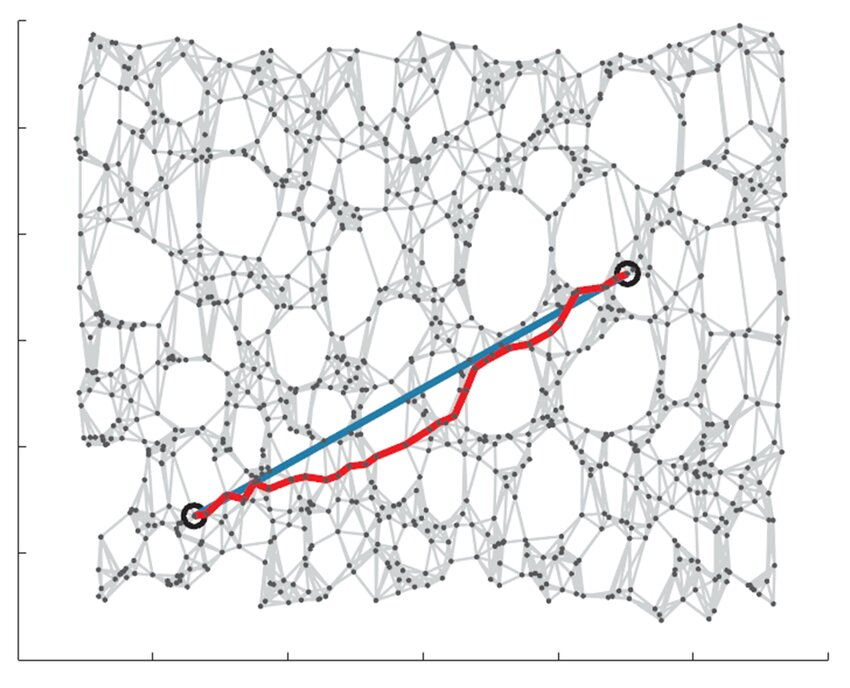
\includegraphics[width=0.8\linewidth]{figure/isomap.png}
    \caption{Isomap算法中的距离为红线长度,相比蓝线的欧氏距离更能体现内蕴性质.}
    \label{fig:iso}
\end{figure}

\subsection{局部线性嵌入（Locally Linear Embedding, LLE）}

LLE是另一种非线性降维方法，强调局部线性结构的保持。它有广泛的应用\cite{roweis2000nonlinear}.

\subsubsection{算法步骤}

\begin{enumerate}
\item \textbf{选择邻域}：
   对每个点$x_i\in\R^n$，找到k近邻$\mathcal{N}(i)$

\item \textbf{计算局部重建权重},其中$W_{ij}$为希望找到的权重：
   \begin{align*}
   \min_W & \sum_{i=1}^n \|x_i - \sum_{j \in \mathcal{N}(i)} W_{ij}x_j\|^2 \\
   \text{s.t.} & \sum_{j \in \mathcal{N}(i)} W_{ij} = 1
   \end{align*}
这里的约束项,从几何上看,保证了在变换$x\mapsto x+c$下目标函数的不变性.

\item \textbf{计算低维嵌入}.求降维后的数据点矩阵$Y\in\R^{n\times k}$,使用一个简单的凸优化：
   \begin{align*}
   \min_Y & \sum_{i=1}^n \|y_i - \sum_{j \in \mathcal{N}(i)} W_{ij}y_j\|^2 \\
   \text{s.t.} & \frac{1}{n}Y^TY = I, \quad \sum_{i=1}^n y_i = 0
   \end{align*}
\end{enumerate}

\begin{remark}
    权重矩阵$W$的求解：
$$
W_i = \frac{C^{-1}\mathbf{1}}{\mathbf{1}^T C^{-1}\mathbf{1}}
$$
其中$C_{jk} = (x_i - x_j)^T(x_i - x_k)$为局部协方差矩阵.
\end{remark}

\subsection{Doubling Dimension and R-Net}

在各种计算几何领域的算法中，我们常常要反复搜索一个点的邻居。在先前的课程中我们提到了可以用LSH来加速这一过程。进一步地，当数据处于一个流形上，我们是否可以使用其他方法来加速这一近邻搜索的过程？

\subsubsection{Doubling Dimension}

倍增维数(Doubling Dimension)是数据内蕴维度的一种。

若对于任意的$p\in P$，$r>0$，有$$\frac{|Ball(p,2r)|}{|Ball(p,r)|}\leq 2^\lambda$$则$\lambda$称为$P$的倍增维数. 一般地，$\R^d$的倍增维数为$\Theta(d)$，但如果数据集$P$分布在一个低维流形上，那么$P$的Doubling Dimension为$\Theta(1)$。对于这样的$P$，我们可以构造一个r-net $Q$来近似。

\begin{definition}[r-net]
给定度量空间$(X,d)$和半径$r>0$，子集$N \subseteq X$称为\emph{r-net}如果满足：
\begin{enumerate}
\item (\textbf{覆盖性}) 对所有$x \in X$，存在$y \in N$使得$d(x,y) \leq r$
\item (\textbf{分离性}) 对所有$y,z \in N$，$d(y,z) \geq r$
\end{enumerate}
\end{definition}

 由定义和三角不等式,有如下结论: 
 \begin{lemma}
对于集合$P$和它的r-net $Q$\[Ball(P,r)\subseteq\bigcup\limits_{\substack{q^\prime\in Ball(q,3r)\\ q^\prime\in Q
     }}Ball(q^\prime,r)\]
 \end{lemma}

根据上述的结论,我们可以将近邻的搜索范围降低到$Q\cap Ball(q^\prime,r)$.

我们有重要的推论:


\begin{lemma}
    设度量空间 $M = (X, \text{dist})$，$S \subset X$，其中 $(S, \text{dist})$ 仍然是一个度量空间。令 $N$ 为 $S$ 的一个 $r$-net，并设 $S$ 的直径为 $D$，则：


\[
|N| \leq (\frac{2D}{r})^{\text{ddim}(M)}
\]

\end{lemma} 


\begin{proof}
    由于 $S \subset X$，我们至少需要 $\lambda(M)$ 个直径为 $D/2$ 的集合覆盖 $S$。每个这样的子集 $S_i \subset S$ 仍然是 $M$ 的子集，因此根据相同的定义，我们可以用 $\lambda(M)$ 个直径为 $D/4$ 的集合覆盖每个 $S_i$。由于有 $\lambda(M)$ 个 $S_i$，总共需要 $\lambda(M)^2$ 个直径为 $D/4$ 的集合覆盖 $S$。

重复这一过程，我们可以覆盖 $S$ 使用：
\begin{itemize}
    \item $\lambda(M)$ 个直径为 $D/2$ 的集合；
    \item $\lambda(M)^2$ 个直径为 $D/4$ 的集合；
    \item $\lambda(M)^3$ 个直径为 $D/8$ 的集合；
    \item ...
    \item $\lambda(M)^{\log_2(\frac{2D}{\lambda})}$ 个直径为$D/2^{\log_2(\frac{2D}{\lambda})} = \frac{r}{2}$。
\end{itemize}

由于 $\frac{r}{2}$ 直径的集合最多只能包含一个 $r$-net 中的点，因此 $N$ 的大小受到以下限制：


\[
|N| \leq \lambda(M)^{\log_2(\frac{2D}{r})} = (\frac{2D}{r})^{\text{ddim}(M)}.
\]


       

\end{proof} 

$r$-net的建立方法: Gonzalez算法.
\begin{enumerate}
    \item 从P中任取一个点$p_1,S=\{p_1\}$
    \item Do $p_j=\textrm{arg}\max d(p_j,S)$, $S=S\cup\{p_j\}$.\\
    While $d(p_j,S)>r$
    \item Return $S$
\end{enumerate}
根据引理5.3, $|S|<(\frac{D}{r})^\lambda$. 时间复杂度为$\Theta((\frac{D}{r})^\lambda nd)$.

\quad

\textbf{问题：如何降低建立r-net的复杂度？}

\quad

Friend List 方法~\cite{har2005fast}. %by Sariel Har-Peled \& Manor Mendel, “Fast Construction of Nets in Low Dimensional Metrics, and Their Applications”。

\quad


\textbf{核心思想}：只在“局部”更新距离，而不是全局扫描。每次加入一个新的center时，那些“距离当前center集合的距离”会产生变化的数据点，只会存在于一些“可能受影响的簇”内。
我们用 friend list 把“可能受影响的簇”限定在常数个(与度量的倍增维度$\lambda$有关)，从而把一次迭代的代价降到 $\lambda^{O(1)}$，而非朴素Gonzalez中的$O(nd)$.

\quad


\textbf{数据结构}：

1.Max heap $H_\alpha$：维护每个数据点$q$到类中心集合$S$的距离$\alpha_q$。（大小为$n$）

2.$C(p_i)$：维护每个类中心$p_i$负责的点集。（总大小为$n$）

3.Friend list $F(p_i)$：与类中心$p_i$距离$\leq 4r_k$的其他\textbf{类中心}。

\quad


\textbf{单次迭代流程}：

1.从$H_\alpha$弹出距离当前类中心集合$S$距离最远的点$p_j$，设其原本所属的类中心是$c$。

2.建立新的类中心$p_j$。

3.局部更新：只扫描两类簇中的所有数据点：\textbf{$c$负责的所有点}、和\textbf{$c$的 friend list中的那些类中心负责的所有点}。对每个需要更新的点$q$，我们重新计算$\alpha_q$，并在需要时把$q$迁入新的簇$C(p_j)$。

4.生成$p_j$的friend list。

\quad


\textbf{时间复杂度改进}：

由于每个类中心的friend list规模最多不超过$O(c'^\lambda)$($c'$为常数)，总的时间复杂度不超过$O(c'^\lambda n\log{n}\log{\frac{D}{r}})$，进一步地，可以将这个复杂度降低至$O(c'^\lambda n\log{n})$。

% 低维嵌入通过求解稀疏特征问题：
% $$
% (I - W)^T(I - W)Y^T = \lambda Y^T
% $$

% \section{比较与应用}

% \begin{table}[h]
% \centering
% \caption{MDS变体方法比较}
% \begin{tabular}{>{\raggedright}p{2cm}>{\raggedright}p{3cm}>{\raggedright}p{3cm}>{\raggedright}p{3cm}}
% \toprule
% \textbf{方法} & \textbf{优点} & \textbf{缺点} & \textbf{适用场景} \\
% \midrule
% 经典MDS & 计算高效，全局结构保持 & 假设数据是欧氏的 & 距离数据可视化 \\
% ISOMAP & 能处理非线性流形 & 计算复杂度高 & 流形学习 \\
% LLE & 保持局部结构，计算相对高效 & 对噪声敏感 & 高维数据可视化 \\
% \bottomrule
% \end{tabular}
% \end{table}
\printbibliography[heading=subbibliography, title={本章参考文献}]
\addcontentsline{toc}{section}{参考文献} % 手动添加到目录
\end{refsection}

\begin{refsection}
    
\chapter{近邻查询}

在高维空间中，近邻查询（Nearest Neighbor Search, NNS）是众多机器学习、计算机视觉与数据检索任务的基础问题。给定一个数据集 $P \subseteq \mathbb{R}^d$ 与查询点 $q \in \mathbb{R}^d$，目标是在 $P$ 中找到与 $q$ 距离最近的点。然而，随着维度 $d$ 的升高，传统的线性扫描方法需要 $O(nd)$ 的时间复杂度，而诸如KD树、R树等低维数据结构的性能在高维下急剧退化，这一现象被称为\textbf{维度灾难（Curse of Dimensionality）}。

为应对该问题，研究者提出了\textbf{近似近邻查询（Approximate Nearest Neighbor, ANN）}，允许返回的解在距离上有一定的近似误差。该思想在工业界（如图像搜索、语音识别、推荐系统）中极为重要，因为牺牲少量精度即可换取数量级的速度提升。

\section{局部敏感哈希}
\quad
局部敏感哈希（Locality-Sensitive Hashing, LSH）的核心思想是\textbf{“相似的点应以较高概率被映射到同一个桶中”}。它通过随机化的哈希函数，将原始高维空间映射到低维哈希空间，使得欧几里得距离或余弦相似度在概率意义下得以保持。
传统的哈希函数通常追求将输入均匀分布，而LSH恰好相反——它希望\textbf{保留数据的局部性}。这种特性使得我们可以通过“哈希冲突”快速过滤出可能的近邻候选点，再进行精确距离计算。

具体来讲，这是一类近似近邻查询(Approx-NN)的方法，其主要思想是设计哈希（Hash）函数，将点集$P$中的点放入不同的桶（Bucket）中，同时使得距离越近的点，其哈希值碰撞的概率越大。最后通过增加hash的次数来提升成功的概率~\cite{earlyhash}。

\quad

\cite{earlyhash}是最早提出 LSH 框架的论文，首次实现了高维空间下的亚线性近似最近邻搜索，为后续研究奠定基础。此后，\cite{pstablehash}一文针对欧几里得距离（L2）设计了一种基于 p-stable 分布 的 LSH 方案，是最常用的实用 LSH 算法之一，适用于图像、音频等连续向量数据。本节聚焦于~\cite{andoni2006near}一文，这是 LSH 理论的里程碑式论文，提出了$(r,R,\alpha,\beta)$-Sensitive Hash的形式定义，并构造出几乎最优的 LSH 结构，显著改善了查询复杂度。该文同时是 LSH 与高维数据结构研究的基础。

\begin{figure}[htbp]
    \centering
    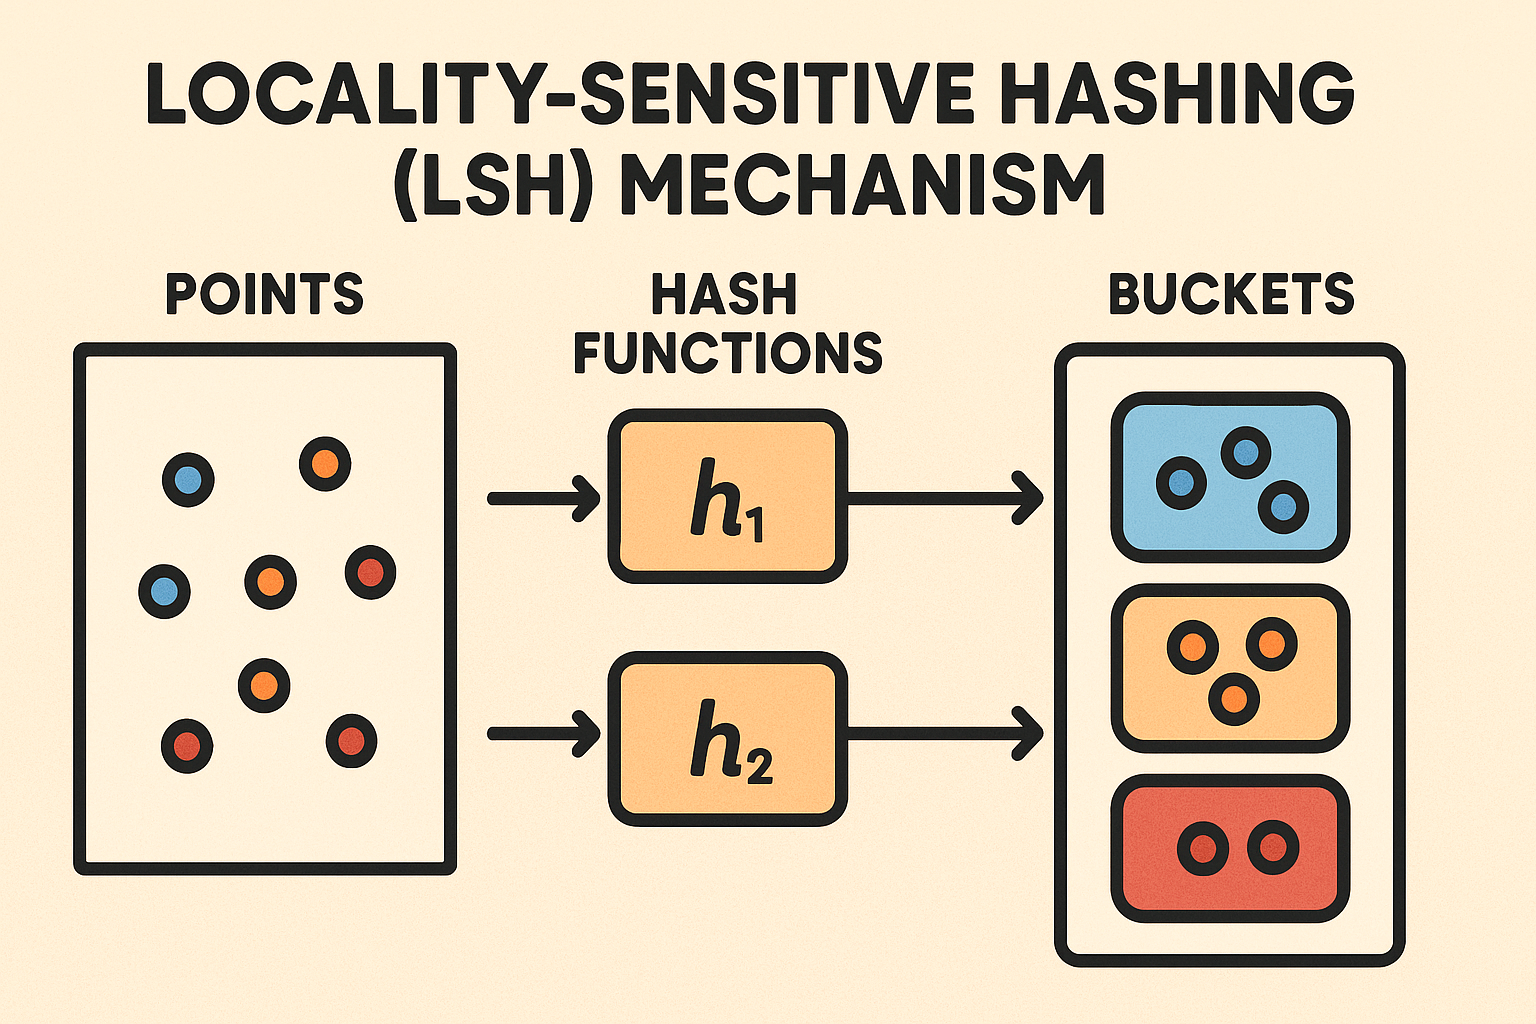
\includegraphics[width=0.8\linewidth]{figure/LSH.png}
    \caption{局部敏感哈希（LSH）}
    \label{fig:LSH}
\end{figure}


\subsection{近似近邻查询}
\begin{definition}[$(r,R)$-近似近邻查询]
    输入集合$P\subset \mathbf{R}^d$ 和 一个点$q\in \mathbf{R}^d$,我们记$dist(q,p)=\mathop{min}_{p\in P}\|q-p\|$。$(r,R)$-近似近邻查询要求
    \begin{enumerate}
        \item  如果$dist(q,P)\leq r$,返回$u\in P$使得$\|q-u\|\leq R$.
        \item 如果$dist(q,P)>R$,输出“$dist(q,P)>r$”.
        \item 如果$r<dist(q,P)\leq R$,返回上面两者中任意一种。
    \end{enumerate}
\end{definition}
上述定义中，$\alpha$ 表示“近点碰撞概率”的下界，而 $\beta$ 表示“远点碰撞概率”的上界。一个好的 LSH 哈希族应当满足 $\alpha \gg \beta$，即在近邻之间有较高的碰撞率，而在远邻之间几乎不会碰撞。参数 $r$ 与 $R$ 控制了“相似”与“不相似”的阈值，二者的比例反映了算法的近似程度。
因此，LSH 的目标可视为通过调整 $(r,R,\alpha,\beta)$ 以及重复哈希的次数 $k$、桶的数量 $\tau$ 来平衡召回率与查询速度。
如果$R=r$，上述问题即为精确的$NS(r)$。通常我们会考虑$R=(1+\epsilon)r$的情况。这个时候我们可以称上面的问题为$(1+\epsilon)$-近似近邻查询。

在已知$dist(q,P)$的上下界为$[a,b]$的情况下，建立集合$U=[a,(1+\epsilon)a,...,(1+\epsilon)^{\log_{1+\epsilon}\frac{b}{a}}a]$,然后对于$r$的选择，我们在$U$上作Binary Search，这样我们可以对通过至多$\log_{1+\epsilon}\frac{b}{a}$次NS(近邻查询)来实现$(1+\epsilon)$-近似近邻查询。

我们用$B(q,r)$表示以$q$为球心，$r$为半径的欧几里得距离的球体。用$N(\Vec{0},I_d)$表示$d$维标准正态分布。$U([a,b])$表示区间$[a,b]$上的均匀随机分布。

\begin{definition}{$(r,R,\alpha,\beta)$-Sensitive Hash~\cite{andoni2006near}}
给定$r<R,1>\alpha>\beta>0$, 我们称$F$是一个$(r,R,\alpha,\beta)$-Sensitive Hash映射集合，如果对于$\forall u,q\in\mathbf{R}^d$,随机取$h\in F$满足
\begin{enumerate}
    \item 如果$u\in B(q,r)$,那么$\Pr[h(u)=h(q)]\geq \alpha$.
    \item 如果$u\not\in B(q,R)$, 那么$\Pr[h(u)=h(q)]\leq \beta$.
\end{enumerate}
\end{definition}
直观地，我们给每个点做“随机投影+分桶”。近的点更容易被分到同一个桶，远的点不太会落在同桶。
如果只用一个哈希函数，误差会比较大；于是把多个哈希“拼在一起”（串联），并且建多张哈希表（并行）。
这样可以做到：近邻命中的概率很高，非近邻几乎不碰撞。
下面我们给一个$F$的构造方法。
考虑这样的$F_T=\{h|h(u)=\lfloor \frac{\langle u,\Vec{v_h} \rangle+t_h}{T} \rfloor\}$,其中$T$是一个待确定的值，$\Vec{v_h}\sim N(\Vec{0},I_d)$,$t_h\sim U([0,T])$.
我们有如下定理
\begin{theorem}
    任给$r,\epsilon>0$,$1>\alpha>\beta>0$,且$\frac{\log\frac{1}{\alpha}}{\log\frac{1}{\beta}}\leq \frac{1}{1+\epsilon}$,则一定存在$T>0$,使得$F_T$是$(r,(1+\epsilon)r,\alpha,\beta)-$Sensitive 的。
\end{theorem}
这一构造的几何直觉是：每个哈希函数 $h(u)=\lfloor \frac{\langle u, v_h \rangle + t_h}{T} \rfloor$ 可看作在高维空间中沿随机方向 $v_h$ 进行“切片”，每个切片宽度为 $T$。若两点 $u,q$ 距离较小，则它们沿该方向的投影 $\langle u,v_h\rangle$ 与 $\langle q,v_h\rangle$ 也相近，从而更可能落入同一切片区间。通过随机采样多个方向并取组合哈希，即可放大这种“近点高碰撞、远点低碰撞”的概率差异。

注意到上面的$h$是将$\mathbf{R}^d\rightarrow \mathbf{Z}$,
下面我们讨论如果将该Hash过程的成功率提高。为此我们考虑一个新的哈希函数$g:\mathbf{R}^d\rightarrow \mathbf{Z}^k$, 其中$g=(h_1,h_2,...,h_k)$,$h_i\in F$.
这样构成的函数族我们称为$G(F,k)={g=(h_1,...,h_k|h_i\in F)}$。那么我们有下面的结论：
\begin{theorem}
       令$\rho=\frac{\log\frac{1}{\alpha}}{\log\frac{1}{\beta}}\leq \frac{1}{1+\epsilon}$, $k=\log_{\frac{1}{\beta}}n$, $\tau=2 n^{\rho}=o(n)$.随机从$G(F,k)$中取出$g_1,g_2,...,g_{\tau}$其对应$\tau$个哈希bucket $H_1,...,H_{\tau}$
       ,我们有对于$\forall q\in \mathbf{R}^d$,满足下列两个条件的概率$\geq \frac{3}{5}$:
       \begin{enumerate}
           \item 如果$\exists u\in P$,使得$\|u-q\|\leq r$,则$\exists j$使得$g_j(u)=g_j(q)$.
           \item 如果$\forall u\in P$, $\|u-q\|>(1+\epsilon)r$,则在$H_1,H_2,...,H_{\tau}$中与$q$发生冲突的点$\leq 4\tau$.
       \end{enumerate}
\end{theorem}
\begin{proof}
    先证明2。
    \begin{align*}
        &\forall u\in P,\|u-q\|>(1+\epsilon)r\\
        &\Rightarrow \forall g\in G(F,k), \Pr[g(u)=g(q)]\leq \beta^k=\frac{1}{n}\\
        &\Rightarrow \forall H_j, \E[\text{发生冲突个数}]\leq 1\\
        &\Rightarrow \text{在}H_1\sim H_{\tau}\text{中发生冲突总数期望}\leq \tau\\
        &\Rightarrow \Pr[\text{发生冲突个数}\leq 4\tau]\geq \frac{3}{4}
    \end{align*}
    再证明1.
    \begin{align*}
        &\|u-q\|\leq r\\
        &\Rightarrow \forall q,\Pr[g(u)=g(q)]\geq \alpha^k=n^{-\rho}\\
        &\Rightarrow H_1\sim H_{\tau}\text{至少发生一次冲突的概率}\geq 1-(1-n^{-\rho})^{\tau}=1-(1-n^{-\rho})^{2n^{\rho}}\geq 1-\frac{1}{\epsilon^2}>\frac{4}{5}.
    \end{align*}
\end{proof}

由该定理，我们可以将$P$中的点分为3个类：
\begin{enumerate}
    \item $\|u-q\|\leq r$,此时发生冲突个数$\geq 1$
    \item $\|u-q\|>(1+\epsilon)r$,此时发生冲突个数$\leq 4\tau$
    \item $r<\|u-q\|\leq (1+\epsilon)r$,此时发生冲突个数可能很多也可能很少，所以返回任意情况
\end{enumerate}
这样我们只需要检查前面$\leq 4\tau+1$个冲突即可。

\quad

\textbf{复杂度与代价分解：}\quad
记 $d$ 为维度、$n$ 为数据量。对常见 $p$-stable LSH，计算一次哈希大致是 $O(d)$。
选取
\[
k\approx \log n,\qquad \tau\approx n^\rho\ \ (0<\rho<1).
\]
则：
\begin{itemize}
  \item \textbf{建表时间}\ $O\big(n\cdot \tau \cdot k \cdot d\big)$：每个点需计算 $\tau$ 组、每组 $k$ 个哈希并入桶。
  \item \textbf{额外空间}\ $O(n\cdot \tau)$（倒排桶指针）$+O(nd)$（若需存原数据）。
  \item \textbf{查询时间}\ 为两部分之和：
  \[
  O(\tau\cdot k\cdot d)\ \ (\text{算哈希、定位桶})
  \ +\ 
  O(\text{候选数}\times d)\ \ (\text{对候选验距}).
  \]
  远点误碰撞在期望/高概率意义下约为 $O(\tau)$，再加近邻常数个真阳性，故整体
  \[
  \tilde O\big(\tau\cdot k\cdot d+\tau\cdot d\big)=\tilde O\big(n^\rho d\big),
  \]
  其中 $\tilde O$ 忽略 $\log n$ 因子。与线性扫描 $O(nd)$ 相比是数量级提升。
\end{itemize}

\subsection{参数选择与实践经验}
在实际应用中，参数 $(k,\tau)$ 的选取直接决定了 LSH 的性能：
\begin{itemize}
  \item 增大 $k$ 会降低单个桶的碰撞概率，但能有效减少误匹配（提高精度）；
  \item 增大 $\tau$ 相当于重复哈希更多次，可提升召回率；
  \item 典型设置中，$k=\Theta(\log n)$，$\tau=\Theta(n^{\rho})$，其中 $\rho=\frac{\log(1/\alpha)}{\log(1/\beta)}$。
\end{itemize}
此外，不同距离度量对应不同的哈希函数族：
\begin{itemize}
  \item \textbf{欧氏距离 $L_2$}：$p$-stable LSH，常用形式 $h_{a,b}(x)=\lfloor(\langle a,x\rangle+b)/T\rfloor$，$a$ 高斯随机、$b$ 均匀随机、$T$ 为桶宽。
  \item \textbf{余弦相似}：随机超平面（Sign Random Projection），比较 $\langle v,x\rangle$ 的符号（$v$ 为随机方向）；夹角越小，哈希一致概率越高。
  \item \textbf{汉明距离}：位采样（bit sampling），直接随机选择若干比特作为哈希。
\end{itemize}
现代工业实现（如 FAISS、Annoy、ScaNN）常结合多层索引、PQ 与 GPU 加速，以在数十亿级别数据上实现毫秒级响应。


% \section{内积量化}
% 尽管 LSH 在理论上提供了近似最近邻的亚线性查询时间，但其在高维空间下仍需大量哈希表与内存。为进一步提升存储效率与查询速度，研究者提出了另一类基于“向量量化（Vector Quantization）”的方法——其中最具代表性的是\textbf{内积量化（Product Quantization, PQ）}。

% \begin{figure}[htbp]
%     \centering
%     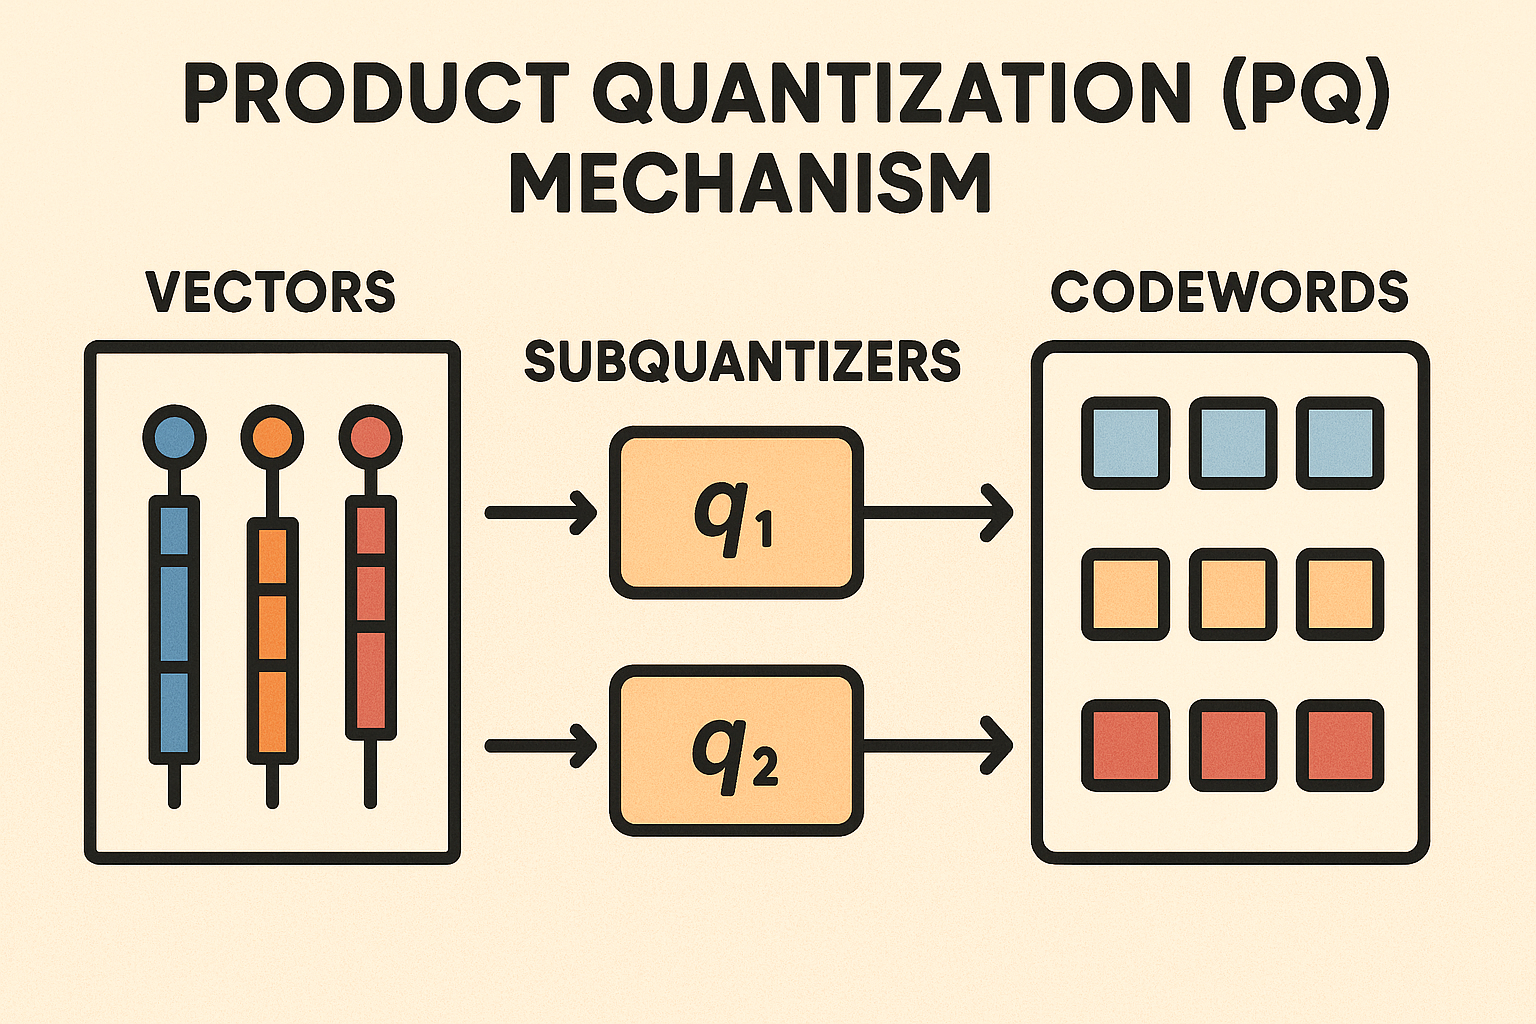
\includegraphics[width=0.8\linewidth]{figure/PQ.png}
%     \caption{内积量化（PQ）}
%     \label{fig:PQ}
% \end{figure}


% \subsection[Product Quantization(PQ)内积量化]{Product Quantization(PQ)内积量化}
% PQ~\cite{5432202}的基本思想是将高维向量空间划分为若干互不重叠的低维子空间，在每个子空间内分别进行 $k$-means 聚类，从而用少量聚类中心组合近似原向量。这样做可以极大地压缩存储空间，因为每个数据点只需记录在各子空间上对应的中心索引（而非完整坐标）。
% 利用$k$-means作近似近邻查询，可以使用$\{c_1,...,c_k\}$来近似$P$,从$\{c_1,...,c_k\}$中找到$u$的最近邻。其查询时间为$\Theta(kd)$.极限情况$k=n$，此时查询时间为$\Theta(nd)$不过可以返回精确解。

% 如果我们将$\mathbf{R}^d$分解为$\mathbf{R}^{\frac{d}{m}}\times \mathbf{R}^{\frac{d}{m}}\times...\mathbf{R}^{\frac{d}{m}}$对于每个$\mathbf{R}^{\frac{d}{m}}$，都存在$P$到其上的投影$P_j,1\leq j\leq m$.我们对于$P_j$做$k$-means,也即找到$\{c_1^j,...,c_k^j\}\subset \mathbf{R}^{\frac{d}{m}}$将所有的中心建立一个"codebook"如下
% \begin{equation}
% CB=\left(
%     \begin{array}{ccc}
%      c_1^1&...&c_k^1  \\
%      ...&...&...\\
%      c_m^1&...&c_m^k 
% \end{array}
% \right)
% \end{equation}
% 该codebook需要空间$k\times m\times \frac{d}{m}=kd$.

% 之后我们建立表$A\in Z^{m\times n}$,其中 第$(i,j)$个元素存储$P$中第$j$个点在第$i$个$\mathbf{R}^{\frac{d}{m}}$子空间上的近似。如果$u$在这$m$个子空间中对应的中心分别为$c^1_{t_1},...,c^m_{t_m}$,那么对于$u$,我们存储列向量$(t_1,...,t_m)^{\top}$在$A$中。

% 之后建立表$B\in \mathbf{R}^{m\times \binom{k}{2}}$,其中第$i$行存储对应的子空间上${c_1^i,...,c_k^i}$中心两两之间的距离。我们用$B_{i,(s_i,t_i)}$表示在第$i$个子空间上$c_{s_i}^i$与$c_{t_i}^i$的距离。

% 我们的算法每次询问一个$q\in \mathbf{R}^d$,首先计算$q$与CB中类中心的距离，得到最近的中心对应的下标列向量$S=(s_1,...,s_m)^{\top}$，将其和A中每一列$T=(t_1,...,t_m)^{\top}$作比较，找到下标距离最近的列。
% 这里的下标距离使用B中得到的对应距离。也即$dist(S,T)=\sum_{i=1}^m{B_{i,(s_i,t_i)}}.$这样的计算可以在$\Theta(m)$时间完成。(这里我们简化了A和B 的存储方式。)
% 输出下标距离最近的列对应的点。


% 这样操作的直觉在于$\forall u,q\in P$ $u=[u_1,...,u_m]$以及$q=[q_1,...,q_m]$
% 我们有
% \begin{align*}
%     \|u-q\|^2&=\sum_{i=1}^m\|u_i-q_i\|^2\\
%     &\approx \sum_{i=1}^m\|c^i_{t_i}-c^i_{s_i}\|^2
% \end{align*}
% 该算法复杂度分析
% \begin{enumerate}
%     \item Construction Time： $T(k-means)+\Theta(mn)+\Theta(k^2m)=\Theta(knd)+\Theta(mn)+\Theta(k^2m)$,如果$k.m\ll n,d$,时间为$\Theta (nd)$
%     \item Space： $\Theta(mk\frac{d}{m})+\Theta(mn)+\Theta(k^2m)=\Theta(n+d)$.
%     \item  Query Time： $\Theta(mk\frac{d}{m})+\Theta(m\times n)=\Theta(n+d)\ll nd$
% \end{enumerate}
% 当然实际使用中还有很多其他的问题，如何存储A，B以及
% 如何优化Codebook? 感兴趣的同学对这些后续问题可以自行了解。

% \quad

% 本节主要聚焦于~\cite{5432202}的工作，这是 PQ 的开创性论文，首次系统提出了将高维向量空间分成子空间、分别进行量化的思想，显著减少存储和计算开销，同时保持良好的近似搜索精度。该方法已成为大规模图像检索的核心技术之一。在PQ被提出之后，\cite{jegou2011searching}提出了 Optimized Product Quantization (OPQ)，通过对原始向量进行旋转变换，使得每个子空间的量化误差更均匀，从而提升 PQ 的整体表示能力和搜索精度。进一步地，\cite{6678503}一文对 OPQ 做了更深入的理论分析和算法优化，实现了更高的准确率和速度平衡。该方法已广泛集成于 Facebook 的 FAISS 库中。
% %%%%%%%%%%% end of doc


\section[Product Quantization (PQ) 乘积量化]{Product Quantization (PQ) 乘积量化}

\paragraph{问题背景与动机}
在近似最近邻（Approximate Nearest Neighbor, ANN）检索中，我们给定一个数据库向量集合
\[
P=\{\mathbf{x}^{(1)},\mathbf{x}^{(2)},\ldots,\mathbf{x}^{(n)}\}\subset \mathbb{R}^d,
\]
其中 $n$ 为数据库规模、$d$ 为向量维度；每次查询给定 $\mathbf{q}\in\mathbb{R}^d$，目标是在 $P$ 中找到使欧氏距离
$\|\mathbf{x}-\mathbf{q}\|_2$ 最小（或近似最小）的向量。\footnote{本文默认使用 $\ell_2$ 距离；常用写法为平方距离 $\|\cdot\|_2^2$，它与 $\|\cdot\|_2$ 在最近邻次序上等价且计算更方便。}

一个最朴素的压缩/加速思路是\emph{向量量化（Vector Quantization, VQ）}：在整个 $\mathbb{R}^d$ 上对 $P$ 做一次 $k$-means，
得到 $k$ 个聚类中心 $\{\mathbf{c}_1,\ldots,\mathbf{c}_k\}\subset\mathbb{R}^d$，并用最近中心近似原向量。
这样每个向量只需存一个中心索引（约 $\log_2 k$ 比特），但查询时若要计算 $\mathbf{q}$ 到所有中心的距离仍需
$\Theta(kd)$ 的代价；同时，为了提高精度需要更大的 $k$，使得训练与查询更昂贵。

\paragraph{PQ 的核心思想：分块量化与“乘积码本”}
Product Quantization（PQ）~\cite{5432202} 的关键思想是：\emph{把高维空间拆成多个互不重叠的低维子空间，
在每个子空间上分别做量化}，从而在总码长固定时获得更强的表示能力。

令 $m$ 为子空间（也称 \emph{子量化器}）个数。为叙述简洁，先假设 $d$ 可被 $m$ 整除，
记子空间维度为 $d' = d/m$。将任意向量 $\mathbf{x}\in\mathbb{R}^d$ 按坐标分块写成
\[
\mathbf{x} = \big[\mathbf{x}_1,\mathbf{x}_2,\ldots,\mathbf{x}_m\big],\quad
\mathbf{x}_i\in\mathbb{R}^{d'}\ (1\le i\le m),
\]
其中 $\mathbf{x}_i$ 表示第 $i$ 个子空间上的子向量（工程上也可用不等长分块或对 $d$ 做零填充，不影响 PQ 思想）。

\textbf{训练阶段（学习子码本）}：对每个子空间 $i$，把数据库向量投影/截取到该子空间得到集合
$P_i=\{\mathbf{x}^{(1)}_i,\ldots,\mathbf{x}^{(n)}_i\}\subset\mathbb{R}^{d'}$，
在 $P_i$ 上做 $k$-means 得到 $k$ 个子中心（子码字）
\[
\mathcal{C}^i=\{\mathbf{c}_1^i,\mathbf{c}_2^i,\ldots,\mathbf{c}_k^i\}\subset\mathbb{R}^{d'}.
\]
将全部子码本记为 $\mathcal{C}=(\mathcal{C}^1,\ldots,\mathcal{C}^m)$。由于整体码字由各子空间码字的\emph{笛卡尔积}
组成，PQ 因而得名“乘积量化”：潜在的全空间码字总数为 $k^m$，但存储与训练仍只需维护 $m$ 个大小为 $k$ 的子码本。

\textbf{码本存储开销}：全部码字向量的总参数量为
$m\times k\times d' = kd$（以浮点数存储时约为 $kd$ 个浮点数）。

\paragraph{编码：将向量映射为 $m$ 个索引}
给定任意数据库向量 $\mathbf{x}$，其 PQ 编码（PQ code）是长度为 $m$ 的索引向量
\[
\mathbf{t}(\mathbf{x})=(t_1,\ldots,t_m)^\top \in [k]^m,\qquad [k]=\{1,2,\ldots,k\},
\]
其中每个子索引由最近子中心给出
\[
t_i \;=\; \arg\min_{1\le j\le k}\ \|\mathbf{x}_i-\mathbf{c}_j^i\|_2^2,\qquad 1\le i\le m.
\]
对应的\emph{重建向量}为
\[
\widehat{\mathbf{x}}=\big[\mathbf{c}_{t_1}^1,\mathbf{c}_{t_2}^2,\ldots,\mathbf{c}_{t_m}^m\big]\in\mathbb{R}^d,
\]
即用每个子空间选中的码字拼接近似原向量。

为了便于整体表示数据库编码，我们把所有编码收集成一个\emph{编码矩阵}
\[
\mathbf{T}\in [k]^{m\times n},
\]
其第 $j$ 列 $\mathbf{T}_{:,j}$ 就是 $\mathbf{x}^{(j)}$ 的 PQ 码（长度为 $m$ 的索引向量）。

\subsubsection{编码长度与存储开销}
每个子空间存一个索引需要 $\log_2 k$ 比特。工程上常取 $k=2^b$（例如 $k=256$，则 $b=8$），
便于用定长整数表示索引。于是每个向量的码长为
\begin{equation}
\mathrm{code\_length} = m\log_2 k\ \text{bits}
\quad(\text{若 } k=2^b,\ \mathrm{code\_length}=mb\ \text{bits}).
\end{equation}
与直接存储 $d$ 维浮点向量相比（例如 32-bit float，共 $32d$ 比特），当 $mb \ll 32d$ 时可显著压缩存储；
代价是引入量化误差，并需要额外存储码本（规模约为 $kd$ 个浮点数）。

\subsubsection{距离估计：对称距离与非对称距离（SDC/ADC）}
PQ 的优势不仅在于压缩，还在于可以用\emph{查表（look-up table）}实现快速距离近似。
对任意 $\mathbf{x},\mathbf{q}\in\mathbb{R}^d$，按相同分块写成
$\mathbf{x}=[\mathbf{x}_1,\ldots,\mathbf{x}_m]$、$\mathbf{q}=[\mathbf{q}_1,\ldots,\mathbf{q}_m]$，则有精确分解
\begin{equation}
\|\mathbf{x}-\mathbf{q}\|_2^2=\sum_{i=1}^m \|\mathbf{x}_i-\mathbf{q}_i\|_2^2.
\end{equation}
PQ 用码字近似子向量，从而把上式近似为“子空间距离之和”。常见两种策略如下。

\begin{itemize}
\item \textbf{对称距离（Symmetric Distance Computation, SDC）}：
数据库向量与查询向量都先量化为码字，再用码字间距离近似。
若 $\mathbf{t}(\mathbf{x})=(t_1,\ldots,t_m)$、$\mathbf{t}(\mathbf{q})=(s_1,\ldots,s_m)$，
则近似距离为
\begin{equation}
\widetilde{d}_{\mathrm{SDC}}(\mathbf{q},\mathbf{x})
=\sum_{i=1}^m \|\mathbf{c}_{s_i}^i-\mathbf{c}_{t_i}^i\|_2^2.
\end{equation}
为加速计算，可为每个子空间预先存储一个 $k\times k$ 的对称距离表
\[
M^{(i)}(a,b)=\|\mathbf{c}_a^i-\mathbf{c}_b^i\|_2^2,\quad 1\le a,b\le k,
\]
则一次距离评估只需 $m$ 次查表与加法，时间为 $\Theta(m)$。缺点是查询也被量化，会额外引入误差。

\item \textbf{非对称距离（Asymmetric Distance Computation, ADC）}：
仅量化数据库向量，查询向量保持为实值，通常精度更好。
对给定查询 $\mathbf{q}$，先在每个子空间预计算其到所有子中心的距离表
\begin{equation}
D_i(j)=\|\mathbf{q}_i-\mathbf{c}_j^i\|_2^2,\quad 1\le i\le m,\ 1\le j\le k.
\end{equation}
那么数据库中任意向量 $\mathbf{x}$（编码为 $\mathbf{t}(\mathbf{x})=(t_1,\ldots,t_m)$）与查询的近似距离可写为
\begin{equation}
\widetilde{d}_{\mathrm{ADC}}(\mathbf{q},\mathbf{x})
=\sum_{i=1}^m D_i(t_i),
\end{equation}
同样可在 $\Theta(m)$ 时间完成一次距离评估；而构建距离表 $\{D_i(\cdot)\}_{i=1}^m$ 的代价为
$\Theta(mkd')=\Theta(kd)$。
\end{itemize}

\paragraph{检索流程（以 ADC 为例）}
\begin{enumerate}
\item \textbf{离线：}学习子码本 $\mathcal{C}$，并把所有数据库向量编码为 $\mathbf{T}\in [k]^{m\times n}$；
\item \textbf{在线查询：}对查询 $\mathbf{q}$ 构建距离表 $D_i(j)$（$1\le i\le m,1\le j\le k$）；
\item \textbf{扫描与排序：}对每个数据库向量的编码列 $\mathbf{T}_{:,j}$，用
$\sum_{i=1}^m D_i(\mathbf{T}_{i,j})$ 计算近似距离并选取最小者（或取 top-$L$ 再精排）。
\end{enumerate}
需要强调的是：若对全部 $n$ 个向量逐一扫描，查询时间为 $\Theta(kd+mn)$，虽然已远小于精确扫描的 $\Theta(nd)$，
但当 $n$ 极大时仍可能过慢。工程中常把 PQ 与倒排文件（IVF）、多级聚类等结构结合（如 IVFADC），
以避免全表扫描并进一步实现亚线性检索；这里先聚焦于 PQ 本身的编码与距离估计机制。

\subsubsection{复杂度分析（训练/存储/查询）}
为更贴近实际，我们在 $k$-means 训练复杂度中显式引入迭代次数 $I$（通常为几十到上百次）。
\begin{enumerate}
\item \textbf{训练（构建）时间：}
需要在每个子空间进行一次 $k$-means。每次迭代对 $n$ 个点、$k$ 个中心计算距离，
子空间维度为 $d'$，因此总时间量级为
\[
\Theta\!\big(m\cdot I\cdot n\cdot k\cdot d'\big)=\Theta\!\big(I n k d\big).
\]
编码数据库（为每个点选择最近子中心）与训练同阶，通常也并入上述量级。

\item \textbf{存储空间：}
子码本存储为 $kd$ 个浮点数；数据库编码为 $m\times n$ 个索引（若 $k=256$ 可用 1 字节存一个索引）。
若使用 SDC，还需存储 $m$ 个 $k\times k$ 距离表，额外为 $\Theta(mk^2)$（通常可用半矩阵或低精度存储）。
因此总空间可写为
\[
\Theta(kd) + \Theta(mn) \quad (\text{可选再加 } \Theta(mk^2)).
\]

\item \textbf{查询时间（ADC，全表扫描）：}
构建查询距离表代价为 $\Theta(kd)$；对每个数据库编码的距离评估为 $\Theta(m)$，
扫描 $n$ 个向量为 $\Theta(mn)$，合计
\[
\Theta(kd + mn),
\]
通常远小于精确扫描的 $\Theta(nd)$。
\end{enumerate}

\paragraph{进一步说明}
PQ 的实际效果与若干工程细节密切相关，例如：（1）索引矩阵 $\mathbf{T}$ 的紧凑存储（字节对齐、SIMD 加速）；
（2）码本训练的初始化与收敛准则；（3）是否对特征做白化/旋转以减少子空间相关性等。
这些内容在后续“优化与工程实现”章节可进一步展开。

\subsection{基于神经网络的乘积量化（Deep/Neural PQ）}
经典 PQ 通常先在固定特征上以无监督方式训练码本（逐子空间 $k$-means），再对数据库进行编码；
近年来另一条重要路线是将“PQ 编码”视为可学习模块，与特征提取网络一起\emph{端到端（end-to-end）}优化，
使得特征、分块方式与码本共同适配下游任务（检索/分类/匹配等）。代表性思路包括：

\begin{itemize}
\item \textbf{端到端监督检索（DPQ）：}
Klein 与 Wolf 的 Deep Product Quantization（DPQ）在监督信号下学习字典式表示，
并同时维护 ``soft'' 与 ``hard'' 两条路径：训练时用软分配保持可导性，推理时用硬编码实现高效检索；
其中硬量化的反向传播常用 \emph{straight-through estimator（STE，直通估计器）}作近似~\cite{klein2019dpq}。

\item \textbf{可导的软分配量化层（PQN/SPQ）：}
Product Quantization Network（PQN）把子空间量化以 ``soft assignment'' 形式嵌入深度网络，
并配合非对称检索目标提升召回~\cite{yu2018pqn}；Self-Supervised PQ（SPQ）在无标签条件下引入自监督目标，
学习更具判别性的 PQ 码~\cite{jang2021spq}。

\item \textbf{用于参数/嵌入压缩的可微 PQ：}
在自然语言处理与推荐系统中，PQ 也可作为可微模块用于压缩大规模 embedding 表；
常见做法是对离散选择做连续松弛（relaxation），或用近似梯度实现端到端训练~\cite{chen2020dpq}.
\end{itemize}

\paragraph{形式化描述：软分配到硬编码}
设神经网络输出特征为 $\mathbf{z}=f_{\theta}(x)\in\mathbb{R}^d$，
同样分块为 $\mathbf{z}=[\mathbf{z}_1,\ldots,\mathbf{z}_m]$，其中 $\mathbf{z}_i\in\mathbb{R}^{d'}$。
对每个子空间学习子码本 $\{\mathbf{c}_1^i,\ldots,\mathbf{c}_k^i\}$。
为保持可训练性，常用带温度参数 $\tau>0$ 的 softmax 产生“软分配概率”
\begin{equation}
p_i(j)=\frac{\exp\!\left(-\|\mathbf{z}_i-\mathbf{c}_j^i\|_2^2/\tau\right)}
{\sum_{\ell=1}^k \exp\!\left(-\|\mathbf{z}_i-\mathbf{c}_\ell^i\|_2^2/\tau\right)},\quad 1\le j\le k,
\end{equation}
其中 $\tau$ 越小，分配越接近 one-hot（更“硬”）。训练时可用
$\sum_{j=1}^k p_i(j)\mathbf{c}_j^i$ 作为连续近似的量化输出；推理时再取硬编码
\[
t_i=\arg\max_{1\le j\le k} p_i(j),
\]
得到最终离散 PQ 码用于检索。

\paragraph{补充：OPQ 与工程库}
本节主要聚焦于~\cite{5432202} 的开创性工作，它首次系统提出了分子空间量化以显著降低存储与计算开销，
并在图像检索等任务中取得良好效果。
在 PQ 提出后，\cite{jegou2011searching} 进一步提出 Optimized Product Quantization（OPQ），
通过对原始向量施加旋转变换，使各子空间量化误差更均匀，从而提升整体表示能力与检索精度。
\cite{6678503} 对 OPQ 做了更深入的分析与优化，实现更好的准确率/速度平衡。
这些方法已广泛集成于 Facebook 的 FAISS 库中，成为大规模向量检索的经典组件。

\printbibliography[heading=subbibliography, title={本章参考文献}]
\addcontentsline{toc}{section}{参考文献} % 手动添加到目录
\end{refsection}



\begin{refsection}
\chapter{次线性算法}
\section{1-median问题}
\textbf{Sublinear Algorithm（次线性算法）}是一类算法~\cite{rubinfeld2011sublinear}，其时间复杂度或空间复杂度小于线性时间$O(n)$或线性空间$O(n)$（其中
$n$ 是输入大小）。这些算法在处理大规模数据时尤为重要，因为它们可以避免遍历整个输入，节省计算资源和存储空间。

\textbf{次线性算法的特点}
\begin{itemize}
    \item 时间复杂度小于$O(n)$: 如$O(logn)$、$n^{\epsilon}$ （其中$0<\epsilon<1$）、$O(1)$等。
    \item 不需要完整读取输入：往往通过随机采样、哈希或其他近似方法，从部分数据中推断整体情况。
    \item 适用于大规模数据：如流数据处理、机器学习、图分析等领域。
\end{itemize}

%#############################################################
%#############################################################
%#############################################################
%#############################################################

\subsection{1-median problem}
``1-median problem''~\cite{indyk1999sublinear}（也叫1-中位数问题或1 median problem）是\textbf{设施选址问题}中的一个经典优化问题。它在运筹学、图论和数据科学中都有广泛应用。

\begin{definition}[1-median problem]
    给定一个加权无向图 \( G = (V, E) \)，其中边的权重 \( w(e) \) 满足三角不等式（即 \( G \) 是一个度量图），顶点数 \( |V| = n \)，边数 \( |E| = \binom{n}{2} \) （即 \( G \) 是一个完全图）。目标是寻找一个顶点 \( v^* \in V \) 使得下式最小化：
\[
S(v) = \sum_{p \in V} w(p, v)
\]
即选取一个顶点，使其到所有其他点的加权距离总和最小。
\end{definition}

\textbf{Goal}:  
找到一个顶点 \( v_0 \in V \)，使得：
\[
S(v_0) \leq (1+\delta) \min\limits_{v \in V} S(v), \quad \delta > 0
\]

\textbf{想象一个 Oracle}: 记作 \( \Gamma_\delta(p, q) \)

\[
\begin{cases}
    S(p) > (1+\delta) S(q) & \text{返回 } q \\
    S(q) > (1+\delta) S(p) & \text{返回 } p \\
    S(p) \leq (1+\delta) S(q) \text{ 且 } S(q) \leq (1+\delta) S(p) & \text{返回 } p \text{ 或 } q
\end{cases}
\]

那么做$n-1$次比较就能得到一个近似最小的顶点：在$V$中的点上构建一个二叉树，每一个叶子节点是点集$V$中的点，每个内部节点对其子节点的函数$S()$值进行比较，并选择较小的那个。将比较质量参数$\delta'$设置为$\delta / \log n$，并将每个比较执行$O(\log n)$次，从而确保所有比较具有较高的正确概率。由于最小元素$S(p)$最多被比较$\log n$次，因此被选元素的值$S(q)$满足$(1 + \delta')^{\log n} \leq 1 + O(\delta)$的界限。接下来就是怎么构造上面这样的一个Oracle，且该Oracle的时间复杂度是常数级别$\Theta(1)$.

\textbf{构造方法：}
分别以$p,q$为顶点，$r$为半径画球，定义$H = \text{Ball}(p, r) \cup \text{Ball}(q, r)$， $t = w(q, p)$， $r = \frac{1}{\delta} t$。 那么分类讨论

(1)对于$\forall v \notin H$，都有\begin{itemize}
    \item $|w(v, p) - w(v, q)| \leq t$
    \item $w(v, p),  w(v, q) \geq \frac{1}{\delta} t$
    \item $\frac{w(v, q)}{w(v, p)}, \frac{w(v, p)}{w(v, q)} \leq \frac{w(v, p) + t}{w(v, q)}= 1 + \frac{t}{w(v, q)} \leq 1 + \delta$
\end{itemize}
所以所有球外的顶点都不考虑。

(2)对于$\forall v \in H$，都有\begin{itemize}
    \item $0 \leq w(v, p) \leq t+r =(1+\frac{1}{\delta})t $
    \item $0 \leq w(v, q) \leq t+r =(1+\frac{1}{\delta})t $
\end{itemize}
根据Hoeffding Bounds。 随机采样$m$个顶点（球内），对应的到顶点$p$的距离为$x_1, x_2, \dots, x_m$。如果我们希望
\begin{equation*}
    \text{Prob}[|\frac{1}{m}\sum_{i=1}^{m}x_{i}- \frac{1}{|H|}\sum_{v\in H}w(p,v)| \geq \epsilon(1+\frac{1}{\delta})t]\leq e^{O(m\epsilon^{2})}=O(\frac{1}{n})
\end{equation*}
那么$m = O(\frac{1}{\epsilon^2}logn)$。因此只需要采样$m$个顶点就能近似$\frac{1}{|H|}\sum_{v\in H}w(p,v)$，使得
\begin{equation*}
    \frac{1}{m}\sum_{i=1}^{m}x_{i} \in \bar{x} \pm \epsilon (1+\frac{1}{\delta})t
\end{equation*}
\begin{equation*}
    \frac{1}{m}\sum_{i=1}^{m}y_{i} \in \bar{y} \pm \epsilon (1+\frac{1}{\delta})t
\end{equation*}
其中$\bar{x} = \frac{1}{|H|}\sum_{v\in H}w(p,v), \bar{y} = \frac{1}{|H|}\sum_{v\in H}w(q,v)$。 

区分$\bar{x}$和$\bar{y}$: 假设 $\bar{x} > \bar{y}$, 那么有
\begin{align*}
    & \bar{x} - \epsilon (1+\frac{1}{\delta})t > \bar{y} + \epsilon (1+\frac{1}{\delta})t \\
    &\Rightarrow \epsilon < \frac{\bar{x}-\bar{y}}{2(1+\frac{1}{\delta})t}
\end{align*}

根据三角不等式有 $\bar{x} + \bar{y} \geq t$， 对$\bar{x}$和$\bar{y}$的取值范围进行分类讨论：\begin{itemize}
    \item (1) $\bar{x}, \bar{y} \geq \frac{1}{3}t$
    \item (2) $\bar{y} \leq \frac{1}{3}t, \bar{x}\geq \frac{2}{3}t$
\end{itemize}

得：
\begin{equation*}
    m = \Theta (\frac{1}{\delta^4}log n)
\end{equation*}

所以，在$\Theta (\frac{1}{\delta^4} n log n)$找到一个顶点 \( v_0 \in V \)，使得：
\[
S(v_0) \leq (1+\delta) \min\limits_{v \in V} S(v), \quad \delta > 0.
\]

\subsection{k-median Problem}
\begin{definition}[k-median]
在集合 $X$ 中寻找 $k$ 个中心点 $c_1, \dots, c_k \in X$，使得以下目标函数的值最小：
\[
\sum_{p \in X} \min_{i = 1, \dots, k} d(p, c_i),
\]
其中 $d(p, c_i)$ 表示点 $p$ 到中心 $c_i$ 的距离。
\end{definition}

我们给出了一个时间复杂度为 $O(n)$ 的 $k$-median 问题近似算法。该方法采用 Korupolu 等人提出的 $(\alpha, \beta)$-近似算法（以下简称 KPR 算法）~\cite{korupolu2000analysis}。令 $s = a\sqrt{kn \log k}$，其中 $a > 1$ 的具体值稍后给出。算法流程如下：

\begin{enumerate}
    \item 从 $X$ 中不放回地随机采样 $s$ 个点，构成集合 $S$；
    \item 在 $S$ 上运行 KPR 的 $k$-median 算法，输出集合 $C' = \{c'_1, \dots, c'_{\beta k}\}$；
    \item 对于每个点 $p \in X$，将其分配给集合 $C'$ 中离它最近的点，令 $d(p, C')$ 表示该距离；
    \item 选取使得 $d(p, C')$ 最大的 $m = b \frac{kn}{\delta} \log k$ 个点构成集合 $M$，其中 $b$ 稍后确定；
    \item 在 $M$ 上运行 KPR 算法，得到输出中心集合 $C''$；
    \item 输出 $C'$ 和 $C''$。
\end{enumerate}

我们设定 $a = \Theta\left( \frac{1}{\delta} \sqrt{\log \frac{1}{\delta}} \right)$，$b = \Theta\left( \frac{1}{\delta^2} \log \frac{1}{\delta} \right)$。算法的总运行时间为  
\[
O\left(k^3 n \log k / \delta^2 \log \frac{1}{\delta} \right)\mathcnperiod
\]

\begin{theorem}
对于任意常数 $\delta > 0$，上述算法以概率 $\Omega(\delta)$ 返回一个  
\[
((1+\delta)3(2+\alpha), 2\beta)
\]
近似解，用于 $k$-median 问题。
\end{theorem}
\begin{proof}
    证明过程详见~\cite{indyk1999sublinear}定理1.
\end{proof}

\section{平均距离问题}
\subsection{平均距离问题}
在几何图（边权$d$可以看作一个度量）$(V,d)$中，时常需要计算平均距离$\sum_{p< q\in V}d(p,q)/\binom{|V|}{2}$. Indyk \cite{indyk1999sublinear} 提出了如下的次线性算法：
\begin{enumerate}
    \item \textbf{独立同分布地以概率$\frac{s}{m}$采样每一条边，得到一个期望大小为$s$的边合$S$}（$n, m$分别是顶点数和边数, $s:=a n$）。
    \item \textbf{计算这些边的平均权重。}
    
\end{enumerate}
由Markov不等式，该随机算法的时间复杂度以很高概率为$O(s)$，主要用于计算算法的第2步。我们的目标是，提出误差为$\delta$的次线性算法，这就需要我们设计$a$的取值。

令$\Delta$为这个图的最大边权。不失一般性，假设最小的边权为1（可以让全部的边权除以之，最后得出结果再乘回来）。对于$0<\epsilon<\delta$, 我们取$c=1+\epsilon$, $I_i=[c^i, c^{(i+1)})$ （这里的上标是指数）。我们按照边权在哪个区间来定量分析：$n_i$定义为边权落在$I_i$的边的个数，$s_i$定义为$S$中边权在$I_i$的边的个数，$\tilde{A}=\sum_{i}c^i n_i, A^\prime =\sum_{e\in S} d(e), \tilde{A}^\prime=\frac{m}{s}\sum_i c^i s_i$. 换句话说，我们用区间的端点取值去逼近真实的平均距离，从而有$A=(1\pm \epsilon)\tilde{A}, A^\prime=(1\pm \epsilon)\tilde{A}^\prime$. 故而，为了得出平均距离，只需证明$\tilde A^\prime$能近似拟合$\tilde A$. 注意到$\tilde A= \Ex{\tilde A^\prime}$，由切比雪夫不等式，为逼近$A$我们只需让方差$D^2(\tilde A^\prime)$尽可能小。

回顾概率论中有指示函数$\mathds{1}_\mathcal{X}(x)=\begin{cases} 
1 & \text{如果 } x \in \mathcal{X}, \\
0 & \text{如果 } x \notin \mathcal{X}
\end{cases}$. 从而有$s_i=\sum_{e: d(e)\in I_i} \mathds 1_{e\in S}$. 由于每条边的采样是独立的，且每条边仅可能落在一个区间$I_i$内，可知$\{s_i: i\in\N_+\}$是一组独立随机变量。因此，
 \begin{align*}
 D^2(\tilde A^\prime)=&D^2(\frac{m}{s}\sum_i c^is_i)&(\text{定义})\\
 =&\frac{m^2}{s^2}D^2(\sum_i c^is_i)&\text{(提取系数)}\\
 =&\frac{m^2}{s^2}\sum_i D^2(c^i s_i)&\text{(独立变量的和的方差)}\\
 =&\frac{m^2}{s^2}\sum_i c^{2i}D^2(\sum_{e: d(e)\in I_i}\mathds 1_{e\in S})& \\
 =&\frac{m^2}{s^2}\sum_i c^{2i}\sum_{e: d(e)\in I_i}D^2(\mathds 1_{e\in S})&\text{(同样是独立变量的和的方差)}\\
 \leq&\frac{m^2}{s^2}\sum_i c^{2i}\sum_{e: d(e)\in I_i}\Ex({\mathds 1^2_{e\in S}})&\text{(对任何随机变量}X,D^2(X)=\Ex X^2-(\Ex X)^2)\\
 =&\frac{m^2}{s^2}\sum_i c^{2i}\sum_{e: d(e)\in I_i}\Pr(e\in S)& \text{(对任何事件$\mathcal{X}$, 恒有}\Ex \mathds 1_\mathcal{X}=\Pr(X))\\
 =&\frac{m^2}{s^2}\sum_i c^{2i}n_i\frac{s}{m}=\frac{m}{s}\sum_i c^{2i}n_i&
 \end{align*}
现在，可以应用切比雪夫不等式，得到
\begin{equation}\label{eq:bad_prob}\begin{aligned}\mathrm{Pr}(|\tilde{A}^{\prime}-E[\tilde{A}^{\prime}]\geq\epsilon\cdot E[\tilde{A}])&\leq\quad\frac{1}{\frac{\epsilon^{2}E^{2}[\tilde{A}^{\prime}]}{D^{2}[\tilde{A}^{\prime}]}}\\&=\quad\frac{D^{2}[\tilde{A}^{\prime}]}{\epsilon^{2}E^{2}[\tilde{A}^{\prime}]}\\
&=\quad\frac{1}{\epsilon^2}\frac{m}{s}F,\end{aligned}\end{equation}

上式的
$F=\frac{\sum c^{2i}n_i}{\sum c^{2i}n_i^2}.$
这是源于
$\Ex [\tilde A^\prime]\geq \sum_i c^{2i}n_i^2$，所以，只需约束$F$的上界.

由于三角不等式，如果$d(a,b)=\Delta,$ 则对任何$p\in V$必有$d(p,a)\geq \frac{\Delta}{2}$ 或 $d(p,b)
\geq \frac{\Delta}{2}$，即每个顶点对应至少一条临边充分长。设最大的非空区间下标为$k=\log_c \Delta$, 则有$k-\log_c 2=\log_c \frac{\Delta}{2}.$ 根据$I_j$的定义对边权大于$\frac{\Delta}{2}$的边计数，有$\sum_{k-\log_c 2\leq j\leq k} n_j\geq n-1$. 由鸽巢原理，存在$k-\log_c 2\leq j\leq k$，使得$n_j\geq\frac{n-1}{\log_c 2}$. 令$P=\{i:N_i\geq t:=\alpha n\}-{j}$, 对应权重充分大的边组成的集合，注意这里的$\alpha$是一个待优化的参数。将$F$记为$\frac{N_1+N_2}{M_1+M_2}$, 而$M_{1}=\sum_{i\in P}c^{2i}n_{i}^{2},M_{2}=\sum_{i\notin P}c^{2i}n_{i}^{2},  N_{1}=\sum_{i\in P}c^{2i}n_{i}, N_{2}=\sum_{i\notin P}c^{2i}n_{i}. $
由定义，$\frac{N_{1}}{M_{1}}\leq\frac{1}{t}$. 
$$  N_{2}\leq t\sum c^{2i}\leq t\frac{c^{2(k+1)}}{c^{2}-1}\leq\frac{\Delta^{2}(1+\epsilon)^{2}}{\epsilon}t $$
 而$ M_{2}\geq(\frac{\Delta}{2}\frac{n-1}{\log_{c}^{2}2})^{2}, $
 故而
 $$ \frac{N_{2}}{M_{2}}\leq\frac{n}{(n-1)^2}\frac{4\log_{c}^{2}2\alpha(1+\epsilon)^{2}}{\epsilon}.$$

从而$F\leq \max(\frac{N_1}{M_1},\frac{N_2}{M_2})$. 设置$\alpha=\Theta(\epsilon^\frac{3}{2})$, 得到$F=O(\epsilon{-\frac{3}{2}}\frac{1}{n})$. 接下来只需根据式\eqref{eq:bad_prob}调整算法输出坏结果的概率：设置$\epsilon=\Theta(\delta), a=O(\delta^{-\frac{7}{2}})$, 我们得到了一个\textbf{常数概率下，时间复杂度为$O(\frac{n}{\delta^\frac{7}{2}})$的$(1+\delta)$-近似算法}。

% \section{k-均值问题}
% 我们想要找到一个算法,使得在次线性时间内,根据输入的度量图$G=(V,E)$,$E$是边权$w$满足三角不等式的边长,且有$\max_{e\in E}w(e)\leq \Delta$,输出


% \cite{czumaj2004sublinear}
\section{k-median问题}
我们首先分析 \textbf{k-中值（k-median）问题}。给定一个有限度量空间 $(V, \mu)$，$V$ 表示点集，$\mu$ 表示两个点间的距离函数。k-中值问题旨在从 $V$ 中选择 $k$ 个中心，使得所有点到其最近中心的距离之和最小。

\vspace{1em}
\noindent\textbf{定义：}
\begin{itemize}
  \item $C = \{c_1, \dots, c_k\} \subseteq V$ 为选出的 $k$ 个中心。
  \item $\mu(v, C) = \min_{1 \le i \le k} \mu(v, c_i)$ 为点 $v$ 到最近中心的距离。
  \item 定义总代价为：
  

\[
    \text{medopt}(V, k) = \min_{C \subseteq V, |C| = k} \sum_{v \in V} \mu(v, C)
  \]


  \item 平均成本为：
  

\[
    \medavg(V, k) = \frac{1}{|V|} \cdot \text{medopt}(V, k)
  \]


  \item 对任意子集 $U \subseteq V$ 和中心集合 $C$，定义其平均代价为：
  

\[
    \text{cost}_{\text{avg}}(U, C) = \frac{1}{|U|} \sum_{v \in U} \mu(v, C)
  \]


\end{itemize}

\subsection{方法概述}
我们研究以下自然采样方案的近似保证：
\begin{enumerate}[label=\textbf{步骤 \arabic*：},leftmargin=*]
    \item 从数据集合$V$中独立均匀随机（i.u.r.）选取大小为$s$的多重子集$S$。
    \item 在样本$S$上运行$\alpha$-近似算法$\mathbb{A}$，得到解$C^*$。
    \item 输出$C^*$作为原问题的近似解。
\end{enumerate}

\subsubsection{分析框架}
\begin{itemize}
    \item \textbf{第一步}：证明$\text{cost}(S, C_{\text{opt}})$能以高概率近似$\text{cost}(V, C_{\text{opt}})$，其中$C_{\text{opt}}$是$V$的最优解。
    \item \textbf{第二步}：由于$C_{\text{opt}}$可能不在$S$中（$k$-中值问题需中心点属于样本），需证明$S$中存在一个可行解，其成本不超过$\frac{c}{\alpha} \cdot \text{cost}(S, C_{\text{opt}})$（$c \geq \alpha$为常数）。
    \item \textbf{关键引理}：若某个解$C$对$V$的成本高于$c \cdot \text{cost}(V, C_{\text{opt}})$，则它要么不是$S$的可行解，要么在$S$上的成本高于$c \cdot \text{cost}(S, C_{\text{opt}})$。
    \item \textbf{结论}：由于算法$\mathbb{A}$返回的解$C^*$在$S$上的成本不超过$c \cdot \text{cost}(S, C_{\text{opt}})$，因此$C^*$对$V$的成本也以高概率不超过$c \cdot \text{cost}(V, C_{\text{opt}})$。
\end{itemize}



在分析具体问题之前，我们先介绍本文中所采用的算法思路：

\vspace{1em}
\noindent \textbf{采样方案} $(V, A, s)$：
\begin{enumerate}[label=\arabic*.]
  \item 从输入集合 $V$ 中独立均匀地采样一个大小为 $s$ 的多重集合 $S$；
  \item 对样本集 $S$，运行某个 $\alpha$-近似算法 $A$ 得到解 $C^*$；
  \item 返回解 $C^*$ 作为最终结果（例如，$k$ 个中心点）；
\end{enumerate}

我们希望分析的问题是：当我们在 $S$ 上运行近似算法 $A$ 时，得到的解 $C^*$ 对原始集合 $V$ 的质量如何？

\vspace{1em}
\noindent \textbf{分析策略分两步：}

\begin{enumerate}[label=\arabic*.]
  \item 我们首先证明，对于给定问题的最优解 $C_{\text{opt}}$，其在 $S$ 上的成本 $\text{cost}(S, C_{\text{opt}})$ 与在 $V$ 上的成本 $\text{cost}(V, C_{\text{opt}})$ 是接近的，具有高概率保证。

  \item 由于 $C_{\text{opt}}$ 不一定是 $S$ 的可行解（例如，$C_{\text{opt}}$ 可能不在 $S$ 中），我们进一步证明：存在一个 $S$ 中的可行解，其成本最多为 $c \cdot \text{cost}(S, C_{\text{opt}})$（$c \ge \alpha$ 为某个常数）。

  由此我们得到：算法 $A$ 会返回成本 $\le c \cdot \text{cost}(S, C_{\text{opt}})$ 的解 $C^*$。

  再结合上述第一步，我们最终得到：
  

\[
    \text{cost}(V, C^*) \le c \cdot \text{cost}(V, C_{\text{opt}})
  \]


  从而保证了该采样算法在全体输入上是 $c$-近似的。
\end{enumerate}




\subsection{主要定理}

\begin{tcolorbox}[colback=gray!5,colframe=black!80!white,title=定理 1]
设 $(V, \mu)$ 是一个度量空间。令 $0 < \delta < 1$、$\alpha \geq 1$、$0 < \beta \leq 1$ 且 $\epsilon > 0$ 为近似参数。设 $\Lambda$ 是一个在度量空间中解决 $k$-中值问题的 $\alpha$-近似算法。如果我们选择一个样本集 $S \subseteq V$，其大小满足



\[
s \geq \frac{c \alpha}{\beta} \left( k + \frac{\Delta}{\epsilon \beta} \left( \alpha \ln\left(\frac{1}{\delta}\right) + k \ln\left( \frac{k\alpha}{\epsilon \beta^2} \right) \right) \right),
\]



其中 $c$ 是某个正的常数，并对样本集 $S$ 运行算法 $\Lambda$，那么对算法得到的解 $C^*$，以下式子以至少 $1 - \delta$ 的概率成立：



\[
\text{cost}_{\text{avg}}(V, C^*) \leq 2(\alpha + \beta) \cdot \text{med}_{\text{avg}}(V, k) + \epsilon\mathcnperiod
\]
\end{tcolorbox}

为了开始分析解 $C^*$ 的近似质量和定理 1 的证明，我们先介绍一些基本符号。

若集合 $C$ 的平均代价满足
  

\[
    \text{cost}_{\text{avg}}(V, C) > (\alpha + \beta) \cdot \medavg(V, k)
  \]


  则称 $C$ 为 $\beta$-坏的 $\alpha$-近似（$\beta$-bad $\alpha$-approximation）。
 否则称其为 $\beta$-好的$\alpha$-近似。

% \subsection*{2.3 引理 1：存在良好样本的概率}

% \textbf{引理 1}：若 $S$ 为大小为


% \[
%   s \ge \frac{3 \Delta \alpha(1+\alpha/\beta) \ln(1/\delta)}{ \beta \cdot \text{medavg}(V, k) }
% \]


% 的独立均匀样本，则 $S$ 中存在中心集合 $C$ 满足


% \[
%   \text{cost}_{\text{avg}}(S, C) \le 2(\alpha + \beta) \cdot \text{medavg}(V, k)
% \]


% 且概率至少为 $1 - \delta$。

% （证明略，使用 Hoeffding 不等式估计样本平均。）

% \subsection*{2.4 引理 2：排除坏近似的概率}

% \textbf{引理 2}：设 $C_b$ 为一个 $6\beta$-坏的 $2\alpha$-近似集合，若样本大小满足


% \[
%   s \ge c \cdot (1 + \alpha/\beta) \cdot \left[ k + \frac{\Delta (\alpha + \beta) \ln(1/\delta) + k \ln(k (\alpha+\beta)\Delta)}{ \beta^2 \cdot \text{medavg}(V,k) } \right]
% \]


% 则满足


% \[
%   \Pr\left[C_b \subseteq S \text{ 且 } \text{cost}_{\text{avg}}(S, C_b) \le 2(\alpha + \beta) \cdot \text{medavg}(V,k) \right] \le \delta
% \]



\begin{lemma}\label{lmm:goodset}
设 $S$ 是一个大小为


\[
s \geq \frac{3\Delta \alpha (1 + \alpha / \beta) \ln(1/\delta)}{\beta \cdot \text{med}_{\text{avg}}(V, k)}
\]


的多重集，从 $V$ 中独立均匀随机选择。

如果一个 $\alpha$-近似算法 $\mathcal{A}$ 在输入 $S$ 上运行，那么对于 $\mathcal{A}$ 返回的解 $C^*$，以下结论成立：


\[
\Pr \left[ \text{cost}_{\text{avg}}(S, C^*) \leq 2(\alpha + \beta) \cdot \text{med}_{\text{avg}}(V, k) \right] \geq 1 - \delta\mathcnperiod
\]

\end{lemma}

\begin{lemma}\label{lmm:bad_set}
 设 $S$ 是从 $V$ 中选出的 $s$ 个点组成的多重集，并满足：



\[
s \geq c \left( (1 + \alpha / \beta)k + \frac{(\alpha + \beta)\Delta \left( \ln(1/\delta) + k \ln \left( \frac{k(\alpha + \beta)\Delta}{\beta^2 \cdot \text{med}_{\text{avg}}(V, k)} \right) \right)}{\beta^2 \cdot \text{med}_{\text{avg}}(V, k)} \right),
\]



其中 $c$ 是某个正的常数。

设 $\mathcal{C}$ 是 $V$ 的 $k$-中值问题中所有 $(2\alpha + 6\beta)$-坏解的集合。则
\[
\Pr \left[ \exists \mathcal{C}_b \in \mathcal{C} \text{ 满足 } \mathcal{C}_b \subseteq S \text{ 且 } \text{cost}_{\text{avg}}(S, \mathcal{C}_b) \leq 2(\alpha + \beta) \cdot \text{med}_{\text{avg}}(V, k) \right] \leq \delta\mathcnperiod
\]


\end{lemma}

上述两个引理的证明参见\cite{czumaj2007sublinear}的section 2. 引理~\ref{lmm:goodset} 保证算法返回的解 $C^*$ 在样本上表现良好，引理~\ref{lmm:bad_set} 保证这样的解 $C^*$ 不会是一个在原问题中表现很差的“伪优解”。

因此，定理 1 能够断言：在适当的采样规模下，样本上运行的近似算法会返回一个在全体数据集上也表现良好的聚类解，而且概率高达 $1 - 2\delta$. 接下来我们给出定理1的证明。


\begin{proof}
 设 $\beta^*$ 是一个将在稍后证明中设定的正参数。设 $s$ 被选择使得引理 2.2 和 2.3 的前提条件在 $\beta$ 被 $\beta^*$ 替换后成立，即
\begin{equation}
s \geq c(1 + \alpha / \beta^*) \left( k + \frac{\Delta}{\beta^* med_{\text{avg}}(V, k)} \left( \alpha \ln(1/\delta) + k \ln \left( \frac{k(\alpha + \beta^*)\Delta}{(\beta^*)^2 med_{\text{avg}}(V, k)} \right) \right) \right)
\end{equation}
对于某个常数 $c$。

设 $S$ 是从 $V$ 中以均匀分布随机选择的 $s$ 个点的多重集。那么根据引理 2.3，以至少 $1 - \delta$ 的概率，没有集合 $C \subseteq S$ 是 $V$ 的 $k$-中值问题的 $(2\alpha + 6\beta^*)$-坏解，同时满足不等式


\[
cost_{\text{avg}}(S, C) \leq 2(\alpha + \beta^*) med_{\text{avg}}(V, k)\mathcnperiod
\]



另一方面，如果我们对集合 $S$ 运行算法 A，则根据引理 2.2，结果集合 $C^*$ 以至少 $1 - \delta$ 的概率满足


\[
cost_{\text{avg}}(S, C^*) \leq 2(\alpha + \beta^*) med_{\text{avg}}(V, k)\mathcnperiod
\]



结合上述结论表明，以至少 $1 - 2\delta$ 的概率，集合 $C^*$ 是 $V$ 的 $k$-中值问题的 $(6\beta^*, 2\alpha)$-好解，即


\[
\Pr \left[ cost_{\text{avg}}(V, C^*) \leq (2\alpha + 6\beta^*) med_{\text{avg}}(V, k) \right] \geq 1 - 2\delta\mathcnperiod
\]



为了完成证明，我们只需要在公式 (5) 中设定参数 $\beta$ 和 $\epsilon$ 并证明 $med_{\text{avg}}(V, k)$ 在 $1/\delta$ 的范围内。

首先我们考虑当 $\text{med}_{\text{avg}}(V, k) \leq \epsilon$ 的情况。我们使用公式 (5) 和 (6)，并令 $\beta^* = \frac{1}{6} \cdot \frac{\epsilon}{\text{med}_{\text{avg}}(V, k)}$。由于 $\beta^* \geq \frac{1}{6}$，那么如果满足条件



\[
s \geq c(1 + \alpha) \left( k + \frac{\Delta}{\epsilon} \left( \alpha \ln \left( \frac{1}{\delta} \right) + k \ln \left( \frac{k(\alpha + 1)\Delta}{\epsilon} \right) \right) \right),
\]



其中 $c$ 是某个正的常数，则以至少 $1 - 2\delta$ 的概率，我们可以得到：



\[
\text{cost}_{\text{avg}}(V, C^*) \leq (2\alpha + 6\beta^*) \cdot \text{med}_{\text{avg}}(V, k) = 2\alpha \cdot \text{med}_{\text{avg}}(V, k) + \epsilon\mathcnperiod
\]



注意这个界限与参数 $\beta$ 无关。

接下来我们考虑当 $\text{med}_{\text{avg}}(V, k) > \epsilon$ 的情况。此时，由公式 (5) 和 (6) 可知，对于某个正的常数 $c$，并令 $\beta = 3\beta^*$，如果满足



\[
s \geq c \left( 1 + \frac{\alpha}{\beta} \right) \left( k + \frac{\Delta}{\beta \epsilon} \left( \alpha \ln \left( \frac{1}{\delta} \right) + k \ln \left( \frac{k\Delta(1 + \alpha / \beta)}{\beta^2 \epsilon} \right) \right) \right),
\]



那么以至少 $1 - 2\delta$ 的概率，我们可以得到：



\[
\text{cost}_{\text{avg}}(V, C^*) \leq 2(\alpha + \beta) \cdot \text{med}_{\text{avg}}(V, k)\mathcnperiod
\]



结合上述两个情况的界限，得证。
\end{proof}

% \subsection*{2.6 小结与讨论}

% \begin{itemize}
%   \item 该分析展示了随机采样在 k-median 问题上的有效性。
%   \item 样本大小可与 $\Delta$、$\alpha$、$k$ 和 $\varepsilon$ 成函数关系，而\textbf{与 $n = |V|$ 无关}。
%   \item 若在 $\mathbb{R}^d$ 中，样本复杂度和误差界还能进一步改进。
% \end{itemize}

\section{亚线性图算法：Sublinear Algorithms for Graphs}

当输入的规模过于庞大时，算法读取全部的输入需要花费大量的时间。因此，我们关心一类算法，只读取输入的极少一部分的信息，就能得到由理论保证的解——亚线性时间算法。
假设输入的规模是$N$，则亚线性时间算法的运行时间只需要$o(N)$。
亚线性时间算法的优良性质来自于对问题的近似以及随机性。特别地，本节课我们学习图数据结构上的亚线性时间算法。

\subsection{背景知识}
由于亚线性算法不能读取完整的输入，算法通过查询对输入进行访问。假设图的顶点集合是已知的，例如$V=\{1,2,\dots,n\}$，
但图的边集是未知的，需要查询。有以下三种标准的\textbf{查询模型}：
\begin{itemize}
    \item 邻接链表查询模型：对任意顶点$u$，可以查询其度数$\deg(u)$，以及它的邻居，可以通过存储一个邻接链表来实现。这个模型更适用于稀疏图。
    \item 邻接矩阵查询模型：对任意的点对$(u,v)$，在$O(1)$的时间内判断它们之间是否连边，可以通过存储一个邻接矩阵来实现。这个模型更适用于稠密图。
    \item 广义查询模型：既可以查询邻接链表，也可以查询邻接矩阵。即：可以查询任意顶点$u$的度数和邻居，也可以查询点对$(u,v)$是否连边。可以通过同时存储邻接链表和邻接矩阵来实现。
\end{itemize}

除此之外，有些算法会允许别的查询，比如边采样的查询，即在查询的时候返回一条均匀随机采样的边。
在接下来的笔记里，我们主要关注邻接链表查询模型。

除了查询模型，亚线性时间算法主要有以下几种\textbf{算法框架}：
\begin{itemize}
    \item 性质检测(Property Testing)：对于图的一些性质，如连通性、是否是平面图等，若图符合该性质，返回Yes；若图\textit{远离}该性质，返回No。
    \item 参数近似(Approximate Parameters)：近似图中的一些参数的\textit{数值}，如最小生成树的权重的值，最大匹配的大小的值等。
    \item 局部计算(Local Computation)：有时我们不只关心图的参数，还关注具体结构，如MST的结构。但光是输出MST就需要$\Omega(n)$的时间了。
    因此，在亚线性时间算法中，我们根据图的局部信息，揭示图的部分结构。例如对于任意一条边，返回其是否属于最小生成树，或者返回其是否属于最大匹配等。
\end{itemize}

前两种框架只输出一个数值，而第三种框架是在我们关心图的某种结构、但又不能花大量时间把结构完全输出时采取的。


\subsection{性质检测}
\textbf{目标：}通过查询模型对图进行访问，要求在尽可能少的查询次数下，判断图$G$是否具有性质$P$，或是\textit{远离}性质$P$。
例如：判断图的连通性，是否是二部图，能否进行3-染色，是否是平面图等。
如果图$G$具有性质$P$，以至少$\frac{2}{3}$的概率接受$G$；如果$G$远离性质$P$，以至少$\frac{2}{3}$的概率拒绝$G$。
对于既不满足$P$又不远离$P$的那部分图，我们不要求算法输出有保证的结果。

以检测图的连通性为例，思考如何辨别以下两种图：

\begin{figure}[!ht]
     \centering
     \begin{subfigure}[T]{0.48\textwidth}
        \centering
        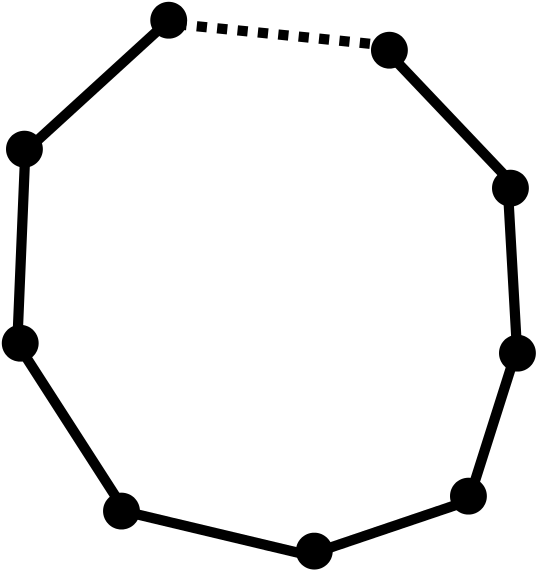
\includegraphics[width=.5\textwidth]{images/cycle.png}
        \caption*{\footnotesize{$G_1$：由$n$个点组成的环}}
     \end{subfigure}
     \hfill
     \begin{subfigure}[T]{0.48\textwidth}
         \centering
         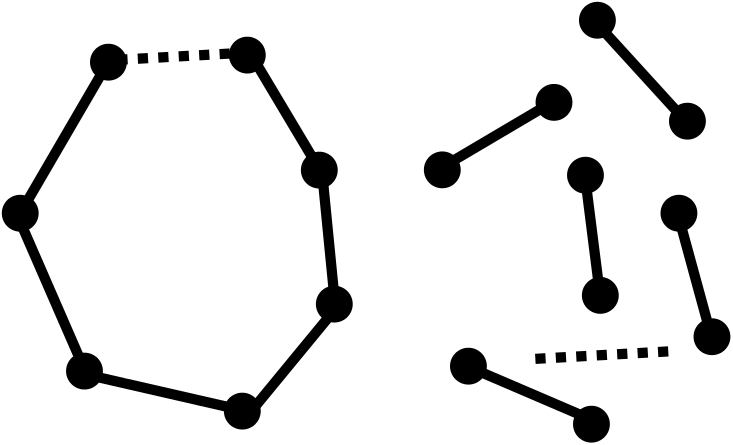
\includegraphics[width=.85\textwidth]{images/far.png}
        \caption*{\footnotesize{$G_2$：一个长为$\frac{n}{2}$的环$+ \frac{n}{4}$条互不相交的边}}
     \end{subfigure}
\end{figure}

为了区分$G_1$和$G_2$，可以采样常数个点（比如采样10个点），然后从采样的这些点出发，做两步广度优先搜索。
如果在搜索的过程中发现了孤立的边，说明是$G_2$，输出No（即不连通）。

\textbf{证明思路：}在$G_2$中，连着孤立边的点有$\frac{n}{4}\cdot 2=\frac{n}{2}$个，占总数的一半，均匀随机地采样10个点，采样的点全都没连到孤立边的概率是$(\frac{1}{2})^{10}$。
只要采样到孤立边对应的点，经过两步广度优先搜索，就一定能判断该图是$G_2$。
因此，以至少$1-\frac{1}{2^{10}}\ge\frac 23$的概率，采样10个点就能区分$G_1$和$G_2$。



如果要精确地判断一个任意的图是否连通，算法至少需要$\Omega(n+m)$次查询，例如，图中只有一个点是孤立的，其余所有点都连通，算法必须找到孤立点，则需要遍历所有的点。
因此，要设计亚线性时间的算法，我们允许算法对图的性质进行近似。



\subsubsection{检测连通性(度数受限图下的邻接链表模型)}
假设图$G$的最大度数是一个常数，记为$d$。远离性质$P$的形式化定义如下：
\begin{definition}
    如果需要对图$G$修改至少$\varepsilon dn$条边才能使得$G$满足性质$P$（修改边之后最大度数仍然是$d$），就称图$G$是$\varepsilon$-远离性质$P$的。
\end{definition}

例如，在\cref{fig:connectivity}中，左图是连通的，而右图更稀疏，需要添加很多条边才能连通，是\textit{远离}连通性的。

\begin{figure}[!ht]
     \centering
     \begin{subfigure}[T]{0.48\textwidth}
        \centering
        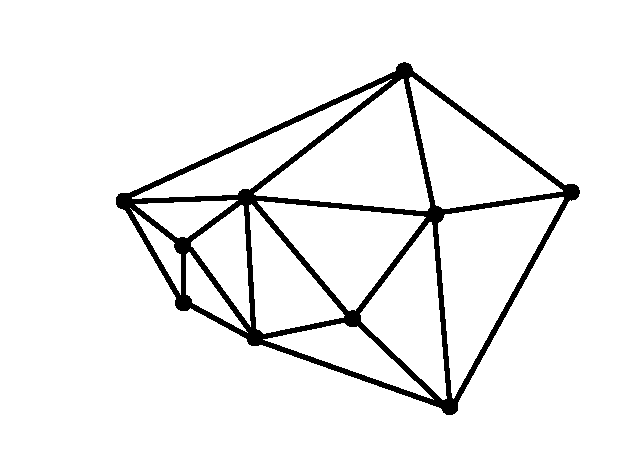
\includegraphics[height=4cm]{images/connected.eps}
	\caption*{连通图}
     \end{subfigure}
     \hfill
     \begin{subfigure}[T]{0.48\textwidth}
         \centering
         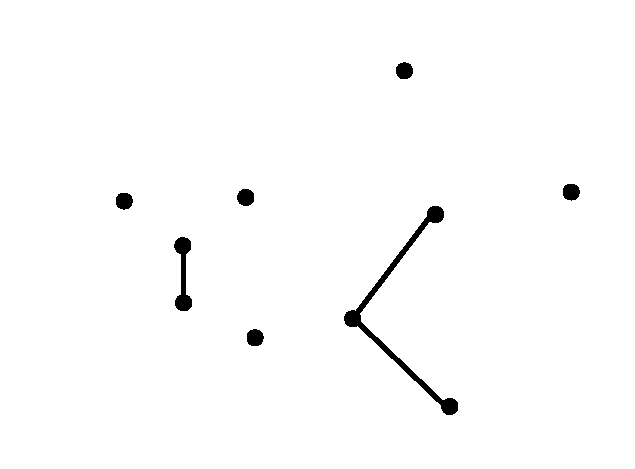
\includegraphics[height=4cm]{images/farconnected.eps}
	\caption*{远离连通性的图}
     \end{subfigure}
     \caption{图的连通性检测}
     \label{fig:connectivity}
\end{figure}

对于远离连通的图，我们观察到：如果一个图是远离连通的，
图中应该有大量较小的连通片（连通片的大小即该连通片包含的点的数量）。
因此我们通过采样一些点，再从这些点出发做广度优先搜索，就能把小的连通片挖掘出来，从而判断图的连通性。
这个观察可以形式化地表现为下面这个断言。
\begin{claim}[\cite{goldreich1997property}]\label{claim:smallCCs}
    如果图$G$是$\varepsilon$-远离连通性，则至少有$\frac{\varepsilon d n}{8}$个连通片的大小是$\le\frac{8}{\varepsilon d}$的。
\end{claim}

\begin{proof}
    记图$G$的连通片数量为$c$。当$G$不连通时，需要添加$c-1$条边才能使其连通（将所有连通片连起来）。
    由于$G$是$\varepsilon$-远离连通性，至少需要修改$\varepsilon dn$条边才能使$G$连通。
    因此，$c-1\ge\varepsilon dn$，即$c\ge\varepsilon dn$。

    记$G$中连通片大小超过$\frac{8}{\varepsilon d}$的数量为$c_1$，
    大小$\le\frac{8}{\varepsilon d}$的连通片的数量为$c_2$，则$c_1+c_2=c$。由于
    \[
    n=\text{$G$中的顶点数}=\sum_{\text{$G$中的连通片$S$}}|S|\ge\sum_{S:|S|>\frac{8}{\varepsilon d}}|S|\ge c_1\cdot\frac{8}{\varepsilon d}
    \]

    所以$c_1\le\frac{\varepsilon dn}{8}$，因此$c_2=c-c_1\ge \varepsilon dn-\frac{\varepsilon dn}{8}\ge\frac{\varepsilon dn}{8}$。
    该断言得证。
\end{proof}

基于以上观察，我们可以设计判断图的连通性的亚线性\textbf{算法}，\textsc{TestingConnectivity}：
\begin{enumerate}
    \item 重复$s=O(\frac{1}{\varepsilon d})$次迭代：
    \begin{enumerate}
        \item[1.1] 均匀随机地采样一个顶点$u$
        \item[1.2] 判断$u$所在的连通片的大小是否较小：
        \begin{enumerate}
            \item[1.2.1] 从$u$出发进行广度优先搜索。如果把$u$所在的连通片都访问完，
            或者已经访问了$t:=\Theta(\frac{1}{\varepsilon d})$个顶点，结束搜索。
            \item[1.2.2] 如果发现了一个大小$<t$的连通片，\textbf{拒绝}图$G$（即认为$G$远离连通性）
        \end{enumerate}
    \end{enumerate}
    \item \textbf{接受}图$G$（即认为$G$是连通的）
\end{enumerate}

\begin{algorithm}[ht]
\caption{\textbf{连通性检测算法}}
	\label{alg-gilbert0}
\begin{enumerate}
    \item \textbf{Input:} 一个整数 $ n \in \mathbb{Z}_{>0} $，$ \epsilon \in (0, 1) $，以及对图 $ G $ 上 $ n $ 个顶点的查询访问。
    \item \textbf{for} $ s := \Theta(1/(d \epsilon)) $ 次 \textbf{do}
    \begin{enumerate}
        \item 从 $ V $ 中随机均匀地抽样一个顶点 $ v $。
        \item 从 $ v $ 开始进行广度优先搜索（BFS），直到到达 $ 2/(d \epsilon) $ 个顶点，或者无法到达新的顶点为止。
        \item \textbf{if} 找到了一个（大小小于 $ n $ 的）连通分量 \textbf{then}
        \begin{enumerate}
            \item 拒绝。
        \end{enumerate}
        \item \textbf{end if}
    \end{enumerate}
    \item \textbf{end for}
    \item 接受。
\end{enumerate}
\end{algorithm}


\begin{theorem}[\cite{goldreich1997property}]
    算法\textsc{TestingConnectivity}能在$O(\frac{1}{\varepsilon^2d})$次查询内，检测图的连通性。
\end{theorem}

\begin{proof}
    \textbf{查询复杂度：}从每个被采样的点出发，广度优先搜索最多访问$\Theta(\frac{1}{\varepsilon d})$个点，
    最多有$\Theta(\frac{1}{\varepsilon d}\cdot d)=\Theta(\frac{1}{\varepsilon})$次查询。
    算法采样了$O(\frac{1}{\varepsilon d})$个点，因此总查询复杂度是$O(\frac{1}{\varepsilon d}\cdot\frac{1}{\varepsilon})=O(\frac{1}{\varepsilon^2 d})$。

    \textbf{正确性：}如果图$G$是连通的，算法\textsc{TestingConnectivity}不会发现大小$<t$的连通片，因此一定会接受$G$。
    如果$G$是$\varepsilon$-远离连通性，令$t=\frac{8}{\varepsilon d}$，则根据\cref{claim:smallCCs}，
    大小$<t$的连通片至少有$\frac{\varepsilon dn}{8}$个，占顶点总数的比例为$\frac{\varepsilon dn}{8}/n=\frac{\varepsilon d}{8}$。
    取$s=2/\frac{\varepsilon d}{8}=\frac{16}{\varepsilon d}$，
    则采样$s$个点均没有落在$<t$的连通片内的概率最多是
    \[
    \left(1-\frac{\varepsilon d}{8}\right)^s<e^{-\frac{\varepsilon d}{8}\cdot s}=e^{-2}<\frac{1}{3}
    \]

    因此，当$G$是$\varepsilon$-远离连通性时，以至少$\frac{2}{3}$的概率，采样的$s$个点中，至少存在一个点所在的连通片大小是$<t$，算法就会拒绝$G$。
\end{proof}

\subsubsection{检测二部性（稠密图上的邻接矩阵模型）}

在本节中，我们展示二分图性质是可用常数查询测试的。我们的算法同样简单明了：我们从顶点集 $ V $ 中抽样一个大小为常数的顶点集 $ S $，通过查询 $ S $ 中所有顶点对，得到诱导子图 $ G[S] $，然后检查该诱导子图 $ G[S] $ 是否为二分图。详见算法\Cref{alg-gilbert}。
\begin{algorithm}[ht]
	\caption{\textbf{二部性检测算法}}
	\label{alg-gilbert}
	\begin{enumerate}
    \item \textbf{Input:} 一个整数 $ n \in \mathbb{Z}_{>0} $，$ \epsilon \in (0, 1) $，以及对图 $ G = (V, E) $ 上 $ n $ 个顶点的查询访问。
    \item 随机均匀地选择一个顶点集 $ S $，其中 $ |S| = \Theta(\epsilon^{-2} \log \epsilon^{-1}) $。
    \item 查询所有顶点对 $ (u, v) $，其中 $ u, v \in S $。
    \item \textbf{if} $ G[S] $ 是二分图 \textbf{then}
    \item \hspace{1em} 接受。
    \item \textbf{else}
    \item \hspace{1em} 拒绝。
    \item \textbf{end if}
\end{enumerate}
\end{algorithm}

\begin{theorem}
\Cref{alg-gilbert}以至少$2/3$的概率成功。
\end{theorem}
\begin{proof}
若 $G$ 是二分图，则其任意导出子图（包括 $G[S]$）也是二分图，因此算法会接受。

现在假设 $G$ 与任意二分图的距离至少为 $\epsilon$（即 $\epsilon$-远）。证明的主要思想如下：  
将采样集 $S$ 划分为两个不交集合 $T$ 与 $U$，其中  
$$
|T| = \frac{4}{\epsilon} \cdot \ln\!\left( \frac{\epsilon}{8/3} \right),
$$
集合 $U$ 由剩余的采样顶点组成。我们首先证明：以高概率，几乎所有顶点都至少有一个邻居在 $T$ 中。暂且假设这一条件成立。

考虑任意一个 $T$ 的二染色 $\chi : T \to \{\text{红}, \text{蓝}\}$。若要将 $\chi$ 扩展为整个图的合法二染色，一个必要条件是：红色顶点的邻居必须是蓝色，蓝色顶点的邻居必须是红色。这样，$T$ 的一个固定染色为 $V \setminus T$ 中的每个顶点施加了一个必要的颜色限制（若某顶点同时邻接红蓝两色顶点，则我们可视作它仅邻接蓝色顶点）。

据此，我们得到一个扩展染色 $\chi'$，它可能合法也可能不合法，但一定满足上述必要条件，且它为 $U$ 中的顶点确定了颜色。由于 $G$ 是 $\epsilon$-远离二分图的，因此在染色 $\chi'$ 下至少有 $\epsilon n^2$ 条单色边。

我们将 $U$ 划分为
$$
\epsilon^2 \cdot \big(|T| + \ln(6)\big)
$$
对（如果有剩余顶点则忽略）。任意一对顶点命中单色边的概率至少为 $\epsilon$，因此所有对都未命中单色边的概率至多为
$$
(1 - \epsilon)^{\epsilon^2 (|T| + \ln 6)} \le \frac{1}{6} \cdot 2^{-|T|}.
$$
因此：
$$
\Pr[\exists\ \text{$T \cup U$ 的合法二染色}] \le
\sum_{\chi \ \text{为}\ T\ \text{的二染色}} \Pr[U\ \text{对}\ \chi' \ \text{无单色边}]
\le 2^{|T|} \cdot \frac{1}{3} \cdot 2^{-|T|} = \frac{1}{3}.
$$

接下来考虑并非每个顶点都有邻居在 $T$ 的情形。定义
$$
\Gamma(T) = T \cup \{ v \in V \setminus T \mid \exists u \in T,\ (u,v) \in E \}.
$$

\begin{claim}
若 $|T| \ge \frac{4}{\epsilon} \ln\!\left( \frac{\epsilon}{8/3} \right)$，则以概率至少 $1 - \frac13$ 有
$$
\sum_{v \notin \Gamma(T)} \deg(v) \le \frac{\epsilon n^2}{2}.
$$
\end{claim}

\begin{proof}
对于度数至少 $\epsilon n/4$ 的顶点 $v$，有
$$
\Pr[v \notin \Gamma(T)] \le (1 - \epsilon/4)^{|T|} \le \frac{\epsilon}{8/3}.
$$
记 $X_v$ 为指示变量，表示事件 $v \notin \Gamma(T)$。则
$$
\mathbb{E}[X_v] \le \frac{\epsilon}{8/3}, \quad
\mathbb{E}\left[ \sum_{v \in V} X_v \right] \le \frac{\epsilon n}{8/3}.
$$
由 Markov 不等式可得
$$
\Pr\left[ \sum_{v \in V} X_v > \frac{\epsilon n}{4} \right] < \frac13.
$$
由于任意顶点度数 $\le n$，可得结论成立。
\end{proof}


假设 $T$ 是好的（即满足上述结论），并取 $T$ 的一个合法二染色 $\chi$。定义扩展染色 $\chi'$ 如下：
$$
\chi'(v) =
\begin{cases}
\chi(v), & v \in T, \\
1, & \exists u \in T, (u,v) \in E, \chi(u) = 2, \\
2, & \text{否则}.
\end{cases}
$$

\begin{claim}
若 $G$ 是 $\epsilon$-远离二分图，且 $\sum_{v \notin \Gamma(T)} \deg(v) \le \frac{\epsilon n^2}{2}$，则在 $\Gamma(T)$ 中由 $\chi'$ 诱导的单色边数超过 $\frac{\epsilon n^2}{2}$。
\end{claim}

\begin{proof}
由于 $G$ 是 $\epsilon$-远离二分图，任何染色 $\chi'$ 都至少有 $\epsilon n^2$ 条单色边。其中至多 $\frac{\epsilon n^2}{2}$ 条与 $V \setminus \Gamma(T)$ 相邻，因此 $\Gamma(T)$ 中的单色边数超过 $\frac{\epsilon n^2}{2}$。
\end{proof}

最后，将 $U$ 划分为
$$
\frac{2}{\epsilon} \cdot \left(|T| + \ln 6\right)
$$
对。由上述引理，每对顶点命中单色边的概率至少为 $\epsilon/2$，因此无对命中单色边的概率至多
$$
(1 - \epsilon/2)^{\epsilon^2 (|T| + \ln 6)} \le \frac{1}{6} \cdot 2^{-|T|}.
$$
综合各项概率估计可知，算法接受的概率至多 $1/3$，因此拒绝的概率至少为 $2/3$。
\end{proof}

\subsection{参数近似}
\textbf{目标：}通过查询模型对图进行访问，要求在尽可能少的查询次数下，比较好地近似图中的一些参数。例如：最小生成树的权重的值，边的数量，最大匹配的大小，给定子图的数量等。

\subsubsection{估算最小生成树的权重}
在本小节中，我们研究近似最小生成树的权重。即：在图$G=(V,E)$中找到一棵树$T\subseteq E$，
使得树的权重$w(T)=\sum_{(u,v)\in T}w(u,v)$最小。最小的权重对应的树记为$T^*$，其权重记为$w(G)=w(T^*)$。
注意到，如果精确地计算最小生成树或者其权重，需要线性的时间，但我们可以在亚线性时间内对其权重进行近似。

\paragraph{最小生成树权重的公式}

\begin{definition}
    记$G^{(\ell)}$表示$G$的子图，$G^{(\ell)}$的顶点集合与$G$相同，
    边集包含$G$中所有权重$\le\ell$的边。记$G^{(\ell)}$中连通片的数量为$c^{(\ell)}$。
\end{definition}

基于上述定义，我们有以下观察：

\begin{claim}\label{claim:MST-CC}
    记$n=|V|$为图$G$的顶点数，$W$表示$G$的最大权重。则$G$中最小生成树的权重满足：$w(G)=n-W+\sum_{i=1}^{W-1}c^{(i)}$。
\end{claim}
\begin{proof}
    记MST中权重为$i$的边的数量为$\alpha_i$，根据Kruskal算法，不同的MST中，$\alpha_i$的值是一样的。
    观察到：
    \begin{itemize}
        \item $\sum_{i=1}^W \alpha_i=n-1$，因为最小生成树上一共有$n-1$条边
        \item 对于任意的$\ell\in[W]$，有$\sum_{i>l}\alpha_i=c^{(\ell)}-1$，因为要想把$G^{(\ell)}$中的所有连通片连起来，
        需要用到$c^{(\ell)-1}$条边，而这些边的权重都$>\ell$，且使用最小生成树上的边就足够把这些连通片连起来了（因为最小生成树是连通的）
        \item $c^{(0)}=n$，因为已经假设图$G$的边权属于$\{1,\dots,W\}$，没有一条边的权重是0，
        因此$G^{(0)}$中没有一条边，每个顶点都是孤立点
    \end{itemize}

    因此，最小生成树的权重可以写成：
    \begin{align*}
        w(G)=&\sum_{i=1}^W i\cdot\alpha_i\\
        &=\sum_{j=1}^W(\sum_{i=j}^W \alpha_i)\\
        &=\sum_{j=1}^W (c^{(j-1)}-1) \tag{利用$\sum_{i>\ell}\alpha_i=c^{(\ell)}-1$}\\
        &=n-W+\sum_{j=1}^{W-1}c^{(j)}
    \end{align*}
\end{proof}

\paragraph{估算连通片的数量}
有了\cref{claim:MST-CC}，我们就只需要估算$c^{(\ell)}$，即每个子图$G^{(\ell)}$的连通片的数量。

对顶点$u$，记$n(u)$表示$u$所在的连通片中顶点的数量。
对任意连通片$A$，观察到：$\sum_{u\in A}\frac{1}{n(u)}=\sum_{u\in A}\frac{1}{|A|}=1$。
进一步，记图$G$的全体连通片的集合为$\cC$，则有：
$\sum_{v\in V}\frac{1}{n(v)}=\sum_{A\in\cC}\sum_{u\in A}\frac{1}{n(u)}=\sum_{A\in\cC}1=|\cC|$，即图中连通片的数量。

因此，如果对每个顶点$v$，$n(v)$的值是已知的，
我们只需要进行简单的操作即可估算连通片的数量：
\begin{enumerate}
    \item 将求和$sum$初始化为0
    \item 重复$s$次迭代：
    \begin{enumerate}
        \item[2.1] 均匀随机地采样一个点$v\in V$
        \item[2.2] 计算$sum\leftarrow sum+\frac{1}{n(v)}$
    \end{enumerate}
    \item 输出$\tilde{c}=n\cdot\frac{sum}{s}$
\end{enumerate}

当然，实际情况中，$n(v)$是未知的，因此我们考虑估算$n(v)$的值。
参考算法\textsc{TestConnectivity}，我们得到一个估算连通片数量的\textbf{算法}$\cA$：
\begin{enumerate}
    \item 将求和$sum$初始化为0
    \item 重复$s=O(1/\varepsilon^3)$次迭代：
    \begin{enumerate}
        \item[2.1] 均匀随机地采样一个点$v\in V$
        \item[2.2] 从$v$出发做广度优先搜索，如果在遍历完整个连通片之前访问了超过
        $\frac{2}{\varepsilon}$个顶点，令$\tilde{n}(v)=\frac{2}{\varepsilon}$；
        
        否则，如果遍历完整个连通片时访问的点数$\le\frac{2}{\varepsilon}$，
        令$\tilde{n}(v)=n(v)$，即访问的点数
        \item[2.3] 计算$sum\leftarrow sum+\frac{1}{\tilde{n}(v)}$
    \end{enumerate}
    \item 输出$\tilde{c}=n\cdot\frac{sum}{s}$
\end{enumerate}

\begin{lemma}\label{lem:appncc}
    对于图$G$，记其连通片的数量为$c$。上述算法$\cA$
    输出的估计值$\tilde{c}$，以至少$\frac{2}{3}$的概率满足$|\tilde{c}-c|\le\varepsilon n$。
    算法$\cA$的运行时间为$O(\frac{d}{\varepsilon^4})$
\end{lemma}
\begin{proof}
    \textbf{运行时间：}对于每个采样的顶点，从它出发探索的点数最多为$\frac{2}{\varepsilon}$，
    由于顶点度数最大是$d$，因此广度优先搜索的时间是$O(\frac{d}{\varepsilon})$。
    因为采样了$O(1/\varepsilon^3)$个顶点，所以总的运行时间为$O(\frac{d}{\varepsilon}/\varepsilon^3)=O(\frac{d}{\varepsilon^4})$。

    \textbf{正确性：}记
    $\hat{n}(u)=\min\{n_u,\frac{2}{\varepsilon}\}$，
    $\hat{c}:=\sum_{u\in V}\frac{1}{\hat{n}(u)}$。
    则：对于任意的顶点$u$，$|\frac{1}{\hat{n}(u)}-\frac{1}{n(u)}|\le\frac{\varepsilon}{2}$。
    因为当$n_u<\frac{2}{\varepsilon}$时，$\hat{n}(u)=n(u)$，此时$\frac{1}{\hat{n}(u)}-\frac{1}{{n}(u)}=0$；
    而当$n_u\ge\frac{2}{\varepsilon}$时，$0<\frac{1}{{n}(u)}\le\frac{1}{\hat{n}(u)}=\frac{\varepsilon}{2}$，
    所以$\frac{1}{\hat{n}(u)}-\frac{1}{{n}(u)}\le\frac{\varepsilon}{2}$。

    因此，有$|\hat{c}-c|=|\sum_{u\in V}\frac{1}{\hat{n}(u)}-\frac{1}{n(u)}|\le\sum_{u\in V}|\frac{1}{\hat{n}(u)}-\frac{1}{{n}(u)}|
    \le\sum_{u\in V}\frac{\varepsilon}{2}=\frac{\varepsilon n}{2}$。

    此外，由于$1\le\hat{n}(u)\le\frac{2}{\varepsilon}$，对任意的$u$，有$\frac{\varepsilon}{2}\le\frac{1}{\hat{n}(u)}\le1$，
    因此$\frac{\varepsilon n}{2}\le\hat{c}\le n$。

    对于第$i$个采样的点，记估计值$\frac{1}{\tilde{n}(u)}$为$X_i\in[0,1]$，计算它的期望：
    $\E[X_i]=\frac{1}{n}\sum_{u\in V}\frac{1}{\hat{n}(u)}=\frac{\hat{c}}{n}$。

    由于$\frac{s}{n}\tilde{c}=\sum_{i=1}^s X_i$，其期望为
    $\E[\sum_{i=1}^s X_i]=s\cdot \E[X_1]=\frac{s\hat{c}}{n}$。
    记$X=\sum_{i=1}^s X_i$，
    根据Chernoff-Hoeffding Bound（见笔记\textit{Notes Lec1 概率论回顾}），有
    \begin{align*}
        \Pr[|\tilde{c}-\hat{c}|\ge\frac{\varepsilon \hat{c}}{2}]&=\Pr[|\frac{s}{n}\tilde{c}-\frac{s}{n}\hat{c}|\ge\frac{\varepsilon}{2}\cdot\frac{s\hat{c}}{n}]\\
        &=\Pr[|X-\E[X]|\ge\frac{\varepsilon}{2}\E[X]]\\
        &\le 2\exp(-\frac{\E[X]\cdot\varepsilon^2/2^2}{3})\\
        &=2\exp(-\frac{s\hat{c}\varepsilon^2}{12n}) \tag{代入$\E[X]$}\\
        &\le2\exp(-O(\frac{1}{\varepsilon^3})\cdot\frac{\varepsilon n}{2}\cdot\frac{\varepsilon^2}{12n}) \tag{由于$s=O(1/\varepsilon^3)$且$\hat{c}\ge\frac{\varepsilon n}{2}$}\\
        &\le\frac{1}{3} \tag{通过选取$s=b/\varepsilon^3$中的常数$b$可以实现}
    \end{align*}

    因此，以至少$\frac{2}{3}$的概率，$|\tilde{c}-c|\le|\tilde{c}-\hat{c}|+|\hat{c}-c|\le\frac{\varepsilon\hat{c}}{2}+\frac{\varepsilon n}{2}\le \varepsilon n$。
\end{proof}

\paragraph{估算最小生成树权重的算法}

根据算法$\cA$，设计估算最小生成树权重的\textbf{算法}$\cB$：
令$\varepsilon'=\frac{\varepsilon}{W}$，再使用median trick增强算法的成功概率，对每个子图$G^{(i)}$调用算法$\cA$得到$\tilde{c}^{(i)}$。
输出$\tilde{w}(G)=n-W+\sum_{i=1}^{W-1}\tilde{c}^{(i)}$。

\begin{theorem}\label{thm:appmst}
    图$G$有$n$个顶点，假设图中每条边的权重都是区间$[1,W]$内的整数，
    则存在一个算法输出估计值$\tilde{w}(G)$，以至少$\frac{2}{3}$的概率满足
    \[
    (1-\varepsilon)\cdot w(G)\le \tilde{w}(G)\le(1+\varepsilon)\cdot w(G)
    \]

    该算法的运行时间为$\tilde{O}(d\cdot W^5/\varepsilon^5)$。
\end{theorem}
\begin{proof}
    根据\cref{lem:appncc}，算法$\cB$得到的任意一个$\tilde{c}^{(i)}$以至少$1-\frac{1}{\poly(W)}$的概率满足$|\tilde{c}^{(i)}-c^{(i)}|\le\frac{\varepsilon n}{W}$。
    因此，利用union bound，对\textit{所有的}$i\in[W]$，该不等式都满足的概率是$1-\frac{1}{\poly(W)}$。下面假设这个事件发生。

    得到$\tilde{w}(G)$的运行时间为
    $W\cdot\tilde{O}(\frac{d}{(\varepsilon/W)^4})=\tilde{O}(\frac{W^5d}{\varepsilon^4})$。
    其理论保证为
    \begin{align*}
        |w(G)-\tilde{w}(G)|&=\left|\left(n-W+\sum_{i=1}^{W-1}{c}^{(i)}\right)-\left(n-W+\sum_{i=1}^{W-1}\tilde{c}^{(i)}\right)\right| \tag{根据\cref{claim:MST-CC}}\\
        &\le\sum_{i=1}^{W-1}|\tilde{c}^{(i)}-c^{(i)}| \\
        &\le(W-1)\frac{\varepsilon n}{W} \tag{根据$\tilde{c}^{(i)}$的理论保证}\\
        &<\varepsilon n\\
        &\le 2\varepsilon\cdot w(G) \tag{由于$c^{(i)}\ge 1$，$w(G)\ge n-W+W-1\ge\frac{n}{2}$，当$n\ge2$时}
    \end{align*}
\end{proof}

\subsubsection{估算图的平均度数}
\problem 对于一个\textbf{连通}的图$G=(V,E)$，其顶点集合为$V=[n]:=\{1,\dots,n\}$。
图中一个点$v$的度数，是和它相连的边数，记为$\deg(v)$。
对图的访问可以是仅允许查询任意顶点的度数，也可以包含查询顶点的邻居。
目标是在亚线性时间内估算图的平均度数，即估算$d_{\avg}=\frac{1}{n}\sum_{v\in V}\deg(v)$。

\paragraph{查询图的度数}
如果只允许查询图中顶点的度数（不允许查询顶点的邻边），这个问题是很难的。

考虑一个星状图$G_1$，即一个中心点连着其他所有顶点，除此之外图中没有别的边。
在这个图里，只有一个顶点的度数是$n-1$，其余顶点的度数都是$1$，
平均度数为$d_{\avg}=\frac{(n-1)\cdot1+1\cdot(n-1)}{n}\approx2$。
要做到2-近似，就一定要访问中心点，否则得到的平均度数是1（2-近似指，算法输出的估算值$R$满足$d_{\avg}\le R\le2d_{\avg}$）。

更进一步，考虑图$G_2$，其中有100个顶点的度数是$n-1$，其余顶点的度数都是1，
平均度数为$d_{\avg}=\frac{(n-100)\cdot1+100\cdot(n-1)}{n}\approx 101$，
那要想做到比100更好的近似比，就需要找到这100个特殊的顶点，需要$\Omega(n)$次查询。
100也可以换成别的常数，这样看来似乎在亚线性时间下，常数近似都做不到。
但$G_2$这样的图是不存在的，因为顶点的度数需要符合图数据结构的规则。

事实上，存在一个亚线性时间的\textbf{算法}\textsc{AvgDeg-V1}，可以做到$(2+\varepsilon)$-近似：
\begin{enumerate}
    \item 调用子程序\textsc{AvgNibble} $t:=\frac{8}{\varepsilon}$次，
    得到估算值$d_{S_1},\dots,d_{S_t}$
    \item 输出这些估算值中的最小值，即输出$R:=\min_{i=1}^t d_{S_i}$
\end{enumerate}

子程序\textsc{AvgNibble}的描述如下：
\begin{enumerate}
    \item 给定某个足够大的常数$\beta>0$，
    采样$s=\frac{\beta\sqrt{n}}{\varepsilon^3}$个点，采样的顶点集合记为$S$
    \item 输出采样的点的平均度数，即输出$d_S:=\frac{\sum_{i\in S}\deg(i)}{s}$
\end{enumerate}


\begin{theorem}\label{thm:avgdeg-v1}
    令$0<\varepsilon<\frac{1}{3}$为一个常数。
    假设算法只允许查询顶点的度数，则\textsc{AvgDeg-V1}算法输出的$R$
    以至少$\frac{3}{4}$的概率满足
    $(\frac{1}{2}-\varepsilon)d_{\avg}\le R\le(1+\varepsilon)d_{\avg}$，
    且运行时间为$O(\sqrt{n}/\varepsilon^4)$。
\end{theorem}

注意到，根据\cref{thm:avgdeg-v1}，有$d_{\avg}\le\frac{1}{1/2-\varepsilon}R\le\frac{1+\varepsilon}{1/2-\varepsilon}d_\avg$，
其中由于$\frac{1}{1-2\varepsilon}\le 1+3\varepsilon$，有
$\frac{1+\varepsilon}{1/2-\varepsilon}\le(2+2\varepsilon)(1+3\varepsilon)=2+O(\varepsilon)$。
令$R'=\frac{1}{1/2-\varepsilon}R$，则$R'$的近似比为$2+\varepsilon$。

为了证明\cref{thm:avgdeg-v1}，需要先证两个引理。

\begin{lemma}\label{lem:nibble-A}
    以至少$1-\frac{1}{1+\varepsilon}\ge\frac{\varepsilon}{2}$的概率，
    算法\textsc{AvgNibble}输出的$d_S$满足$d_S\le(1+\varepsilon)\cdot d_\avg$。
\end{lemma}
\begin{proof}
    令$X_i$表示第$i$个采样的点的度数，由于是均匀随机采样，
    有$\Pr[\text{第$i$个被采样到的顶点为}j]=\Pr[X_i=\deg(j)]=\frac{1}{n}$，。
    因此，
    \[
    \E[X_i]=\sum_{j=1}^n\deg(j)\Pr[X_i=\deg(j)]=\sum_{j=1}^n\deg(j)\cdot\frac{1}{n}=d_\avg
    \]

    由于$d_S=\frac{\sum_{i\in S}\deg(i)}{s}$，
    有$\E[d_S]=\E[\frac{1}{s}\sum_{i=1}^sX_i]=d_\avg$。
    根据Markov不等式，
    \[
    \Pr[d_S>(1+\varepsilon)d_\avg]\le\frac{\E[d_S]}{(1+\varepsilon)d_\avg}=\frac{1}{1+\varepsilon}
    \]
\end{proof}

\begin{lemma}\label{lem:nibble-B}
    以至少$1-\frac{\varepsilon}{64}$的概率，
    算法\textsc{AvgNibble}输出的$d_S$满足$d_S\ge(\frac{1}{2}-\varepsilon)\cdot d_\avg$。
\end{lemma}
\begin{proof}
    对于图$G=(V,E)$，定义$H$为度数最高的$\sqrt{\frac{\varepsilon}{2}n}$个顶点的集合，
    $L=V\setminus H$。

    首先，由于$\sum_{i=1}^n\deg(i)=2|E|$，则$L$和$H$之间的边满足
    $|E(L,H)|\le|E|\le\frac{1}{2}\sum_{i=1}^n\deg(i)$。

    其次，由于$H$中只有$\sqrt{\frac{\varepsilon}{2}n}$个顶点，所以
    $2|E(H)|\le|V(H)|^2=\frac{\varepsilon n}{2}$。

    此外，由于图$G$是连通的，至少有$n-1$条边，所以$\sum_{i=1}^n\deg(i)=2|E|\ge2(n-1)$。
    因此，有
    \[
    2|E(H)|\le\frac{\varepsilon}{2}n\le\frac{\varepsilon}{2}2(n-1)
    \le\frac{\varepsilon}{2}\cdot\sum_{i=1}^n\deg(i)
    \]

    $L$中的点的度数之和满足$\sum_{i\in L}\deg(i)=\sum_{i=1}^n\deg(i)-|E(L,H)|-2|E(H)|$。
    记$L$中顶点的平均度数为$d_L$，则有
    $d_L=\frac{\sum_{i\in L}\deg(i)}{|L|}\ge\frac{(\frac{1}{2}-\frac{1}{2}\varepsilon)\sum_{i=1}^n\deg(i)}{n}=(\frac{1}{2}-\frac{1}{2}\varepsilon)d_\avg$。

    由于这个引理在求$d_S$的下界，我们可以假设所有采样到的顶点都来自$L$。
    定义$D_H$为$H$中最小的度数，$X_i$为第$i$个被采样到的顶点的度数。
    则$\E[X_i]\ge d_L=\frac{\sum_{i\in L}\deg(i)}{|L|}\ge(\frac{1}{2}-\frac{1}{2}\varepsilon)d_\avg$。
    
    由于$d_S=\frac{\sum_{i=1}^sX_i}{s}$，则$E[d_S]=\frac{1}{s}\E[\sum_{i=1}^sX_i]\ge(\frac{1}{2}-\frac{1}{2}\varepsilon)d_\avg$。
    等价地，有$(\frac{1}{2}-\varepsilon)d_\avg\le\frac{\frac{1}{2}-\varepsilon}{\frac{1}{2}-\frac{1}{2}\varepsilon}\E[d_S]\le(1-\varepsilon)\E[d_S]$。

    另一方面，对于平均度数，有$d_\avg=\frac{1}{n}\sum_{i=1}^n\deg(i)\ge\frac{\sum_{i\in H}\deg(i)}{n}\ge\frac{D_H\cdot|H|}{n}$，
    因此$\E[d_S]\ge\frac{(\frac{1}{2}-\frac{1}{2}\varepsilon)D_H\cdot|H|}{n}$，
    且$\E[\sum_{i=1}^sX_i]\ge\frac{(\frac{1}{2}-\frac{1}{2}\varepsilon)D_H\cdot|H|\cdot s}{n}$。
    根据Chernoff Bound，有
    \begin{align*}
        \Pr[d_S\le(\frac{1}{2}-\varepsilon)d_\avg]&\le\Pr[d_S\le(1-\varepsilon)\E[d_S]]\\
        &=\Pr[\frac{1}{s}\sum_{i=1}^sX_i\le(1-\varepsilon)\frac{1}{s}\E[\sum_{i=1}^sX_i]]\\
        &=\Pr[\frac{1}{D_H}\sum_{i=1}^sX_i\le(1-\varepsilon)\frac{1}{D_H}\E[\sum_{i=1}^sX_i]]\\
        &\le2\exp(\frac{-\E[\sum_{i=1}^sX_i]\cdot\varepsilon^2}{3\cdot D_H}) \tag{假设采样的点都来自$L$，有$0\le\frac{X_i}{D_H}\le1$}\\
        &\le2\exp(\frac{-s\cdot|H|}{n}\cdot(\frac{1}{2}-\frac{1}{2}\varepsilon)\cdot\frac{\varepsilon^2}{3})\\
        &\le2\exp(\frac{-s\cdot \varepsilon^{2.5}}{100\sqrt{n}})
    \end{align*}

    因此，令$s=\frac{200\sqrt{n}}{\varepsilon^3}$，即有
    $\Pr[d_S\le(\frac{1}{2}-\varepsilon)d_\avg]\le\frac{\varepsilon}{64}$。
\end{proof}

有了\cref{lem:nibble-A}和\cref{lem:nibble-B}，我们就能证得\cref{thm:avgdeg-v1}。

\begin{proof}[\cref{thm:avgdeg-v1}的证明]
    首先，根据\cref{lem:nibble-B}，以及$(1-\frac{1}{x+1})^x\ge\frac{1}{e}$，有：
    \[
    \Pr[R\ge(\frac{1}{2}-\varepsilon)]=\Pr[\forall i\in[t],d_{S_i}\ge(\frac12-\varepsilon)d_\avg]
    \ge(1-\frac{\varepsilon}{64})^{\frac{8}{\varepsilon}}>\frac{7}{8}
    \]

    其次，根据\cref{lem:nibble-A}，以及$(1-\frac{1}{x})^x\le\frac{1}{e}$，有：
    \begin{align*}
        \Pr[R\le(1+\varepsilon)d_\avg]&=\Pr[\exists i\in[t], d_{S_i}\le(1+\varepsilon)d_\avg]\\
        &=1-\Pr[\forall i\in[t], d_{S_i}>(1+\varepsilon)d_\avg]\\
        &>1-(1-\frac{\varepsilon}{2})^t\\
        &>1-\frac{1}{16}
        \end{align*}
\end{proof}


\paragraph{查询图的度数和边}
如果算法同时可以访问顶点的度数和邻边，估算平均度数就会容易很多。
在之前的$G_1$的例子中，只能访问顶点度数的算法必须要发现度数为$n-1$的顶点，
才能实现2-近似。但如果算法能访问顶点的邻边，就能很容易地发现度数较高的顶点。

首先先假设一个更简单的情况：假设图$G$是一个几乎正则的图，图中顶点的度数相差不大，
每个顶点的度数都属于区间$[d,10d]$，没有奇异点（即少数点的度数特别大，达到$O(n)$的级别）。
这样的话，算法可以采样一些顶点，计算它们的平均度数。\textbf{算法}描述如下：

\begin{enumerate}
    \item 令$k=\frac{50}{\varepsilon^2}\cdot\ln(\frac{2}{\delta})$，
    \item 对于$i=1,\dots,k$：
    \begin{enumerate}
        \item[2.1] 均匀随机地采样一个顶点，记为$v_i$
        \item[2.2] 令$X_i=\deg(v_i)$
    \end{enumerate}
    \item 输出$\tilde{d}=\frac{1}{k}\sum_{i=1}^kX_i$
\end{enumerate}

\begin{claim}
    上述算法输出的估算值$\tilde{d}$满足$\E[\tilde{d}]=d_\avg$。
\end{claim}

\begin{claim}
    上述算法输出的估算值$\tilde{d}$满足$\Pr[|\tilde{d}-d_\avg|\le\varepsilon d_\avg]\ge1-\delta$，
    且运行时间为$O(\frac{1}{\varepsilon^2}\log\frac{1}{\delta})$。
\end{claim}

在几乎正则的图里，顶点度数的方差很小，因此采样法很有效；
但在一般的图里，有些顶点度数很高，使得方差很大。
如果仍然用最简单的采样法来估计，需要的运行时间是$O(\frac{n}{\varepsilon^2}\cdot\log\frac{1}{\delta})$。

\idea 我们可以考虑减小度数高的顶点带来的方差。由于图的边数是有限的（$|E|=m$），度数很高的顶点不会太多，
我们可以通过引入$\deg^+(v)$，把每条边分配给度数较低的点，从而减小高度数顶点的影响。

具体来说，先定义一个偏序关系$\prec$：如果$\deg(u)<\deg(v)$，或者$\deg(u)=\deg(v)$且$\ID(u)<\ID(v)$，
则称$u\prec v$。
其中，$\ID(v)$表示顶点$v$在集合$V$中的字典序，是输入给定的顺序。
接着，定义$\deg^+(u):=\#\{v\in N(u)|u\prec v\}$，即$u$的邻居中满足$u\prec v$的顶点数。
那么：$\sum_{v\in V}\deg^+(v)=m=\frac{n}{2}\cdot d_\avg$。

尽管一般图中的$\deg(v)$的确会非常大，从而带来很大的方差；
但我们将证明，$\deg^+(v)$对每个顶点$v$来说都是有界的，因此方差更小，
估算$\deg^+(v)$能有更好的理论保证。

\begin{definition}
    定义$H\subset V$是在偏序关系$\prec$下前$\sqrt{2m}$大的顶点集合。
    定义$L:=V\setminus H$。
\end{definition}

\begin{claim}\label{claim:LH-bound}
    对任意顶点$v\in H$，有$\deg^+(v)\le\sqrt{2m}$。

    对任意顶点$v\in L$，有$\deg(v)\le\sqrt{2m}$。
\end{claim}
\begin{proof}
    对于任意$H$中的顶点$v$，$\deg^+(v)$只包含在偏序关系$\prec$下比$v$大的顶点，
    一定也属于$H$，所以$\deg^+(v)\le|H|=\sqrt{2m}$。

    另一方面，对于任意$L$中的顶点$v$，假设$\deg(v)>\sqrt{2m}$，
    那么满足$\deg(u)\ge\deg(v)>\sqrt{2m}$的点$u$一定落在$H$里，
    数量至少是$|H|=\sqrt{2m}$个。则图中的边数
    \[
    m=\frac{1}{2}\sum_{i=1}^n\deg(i)
    \ge\frac{1}{2}\sum_{u:\deg(u)>\deg(v)}\deg(u)
    >\frac{1}{2}\sqrt{2m}\cdot\sqrt{2m} =m
    \]

    出现了矛盾，假设不成立。因此，对任意$v\in L$，有$\deg(v)\le\sqrt{2m}$。
\end{proof}

下面描述\textbf{算法}\textsc{AvgDeg-V2}：
\begin{enumerate}
    \item 令$k=\frac{16}{\varepsilon^2}\cdot\sqrt{n}$
    \item 对于$i=1,\dots,k$：
    \begin{enumerate}
        \item[2.1] 从集合$V$中均匀随机地采样一个点，记为$v_i$
        \item[2.2] 从$v_i$的邻居集合$N(v_i)$中均匀随机地采样一个点，记为$u_i$
        \item[2.3] 如果$v_i\prec u_i$，令$X_i=2\cdot\deg(v_i)$；
        否则，令$X_i=0$
    \end{enumerate}
    \item 输出$R:=\frac{1}{k}\sum_{i=1}^kX_i$
\end{enumerate}

下面这个定理描述了算法\textsc{AvgDeg-V2}的理论保证。

\begin{theorem}
    令$0<\varepsilon<\frac{1}{3}$为一个常数。如果算法能访问顶点的度数和邻边，
    那么算法\textsc{AvgDeg-V2}输出的估算值$R$以至少$\frac{3}{4}$的概率满足
    $(1-\varepsilon)d_\avg\le R\le(1+\varepsilon)d_\avg$，
    且算法的运行时间为$O(\sqrt{n}/\varepsilon^2)$。
\end{theorem}

\begin{proof}
    
\textbf{证明思路：}令$X=\sum_{i=1}^kX_i$，先证明$\E[X]=d_\avg$（是无差估计），且方差很小。
接着用Chebyshev不等式证明估算值$R:=\frac{1}{k}X$的误差很小。

\textbf{证均值：$\E[X_1]=d_\avg$.} 由于是均匀随机采样，每个$X_i$之间是独立的，均值和方差相同，分析$X_1$即可。
\begin{align*}
   \E[X_1]&=\sum_{v\in V}\frac{1}{n}\E[X_1|v\text{被采样}]\\
   &=\sum_{v\in V}\frac{1}{n}\sum_{u\in N(v)}\frac{1}{\deg(v)}\E[X_1|v,u\text{被采样}]\\
   &=\sum_{v\in V}\frac{1}{n}\left(\sum_{u\in N^+(v)}\frac{1}{\deg(v)}\cdot2\deg(v)+ \sum_{u\notin N^+(v)}\frac{1}{\deg(v)}\cdot0\right) \tag{其中，$N^+(v)=\{u\in N(v)|v\prec u\}$}\\
   &= \sum_{v\in V}\frac{2\deg^+(v)}{n}\\
   &= \frac{2m}{n} \tag{根据$\sum_{v\in V}\deg^+(v)=m$}\\
   &= d_\avg
\end{align*}

\textbf{证方差：$\Var[X_1]\le 4\sqrt{2m}\cdot d_\avg$.}
\begin{align*}
    \Var[X_1]&\le\E[X_1^2]\\
    &=\sum_{v\in V}\frac{1}{n}\sum_{u\in N(v)}\frac{1}{\deg(v)}\E[X_1^2|v,u\text{被采样}]\\
    &=\sum_{v\in V}\frac{1}{n}\sum_{u\in N^+(v)}\frac{1}{\deg(v)}(2\deg(v))^2\\
    &=\sum_{v\in V}\frac{4\deg(v)\cdot\deg^+(v)}{n}\\
    &=\frac{4}{n}\left(\sum_{v\in H}\deg(v)\cdot\deg^+(v)+\sum_{v\in L}\deg(v)\cdot\deg^+(v)\right) \tag{因为$V=H\cup L$}\\
    &\le\frac{4}{n}\left(\sum_{v\in H}\deg(v)\cdot\sqrt{2m}+\sum_{v\in L}\sqrt{2m}\cdot\deg(v)\right) \tag{根据\cref{claim:LH-bound}，且$\deg^+(v)\le\deg(v)$}\\
    &\le 4\sqrt{2m}\cdot d_\avg \tag{由于$\frac{\sum_{v\in H}\deg(v)+\sum_{v\in L}\deg(v)}{n}=\frac{\sum_{v\in V}\deg(v)}{n}=d_\avg$}
\end{align*}

由于$R=\frac{1}{k}\sum_{i=1}^kX_i$，有
$\Var[R]=\frac{1}{k}\Var[X_1]\le\frac{4\sqrt{2m}\cdot d_\avg}{\frac{16}{\varepsilon^2}\sqrt{n}}=\frac{\varepsilon^2\sqrt{d_\avg}\cdot d_\avg}{4}$。

\textbf{Chebyshev不等式：}
\[
\Pr[|R-d_\avg|\ge\varepsilon\cdot d_{\avg}]\le\frac{\Var[R]}{\varepsilon^2d_\avg^2}
\le\frac{\varepsilon^2\sqrt{d_\avg}\cdot d_\avg}{4\varepsilon^2\cdot d_\avg^2}
\le\frac{1}{4}
\]

因此，$\Pr[|R-d_\avg|\le\varepsilon\cdot d_\avg]\ge\frac{3}{4}$。

\textbf{运行时间：}对每一轮迭代，采样顶点$v_i$和$u_i$只需要$O(1)$的时间，因此总的运行时间为$O(k)=O(\frac{\sqrt{n}}{\varepsilon^2})$。
\end{proof}


\printbibliography[heading=subbibliography, title={本章参考文献}]
\addcontentsline{toc}{section}{参考文献} % 手动添加到目录
\end{refsection}


\begin{refsection}
\chapter{VC维与核心集}
\section{VC维简介}
VC Dimension（Vapnik-Chervonenkis Dimension）是衡量一个假设类（hypothesis class）表达能力和复杂度的重要工具。它由统计学习理论的奠基人Vladimir Vapnik和Alexey Chervonenkis提出\cite{vapnik1971theory}，用于分析机器学习模型的泛化能力。对于SVM问题，我们希望找到一个具有最大间隔的分类超平面，从而将正负样本分离开，但是，我们在训练数据集上得到的一个良好的分类超平面，如何能在新的测试数据点上较好的分类呢？对于图片识别或者人脸识别任务，我们的训练数据集总归是有限的，但是现实世界的图片或者人脸却可以是无穷多的，那么我们怎么能保证在有限数据集上训练的模型能很好的针对无穷的现实世界的数据呢？VC dimension为以上这些问题提供了理论保证，它描述了一个模型能够“完美拟合”的最复杂数据集的大小。VC dimension越高，模型的拟合能力越强，但也可能更容易过拟合；VC dimension越低，模型更简单，但可能欠拟合。


\subsection{基础知识}

\begin{definition}[Range Space]
    Range Space是一个二元组$\Sigma = (X,R)$，其中$X$是一个有限或者无限的集合，称为Ground Set，$R$ = $\{ r \mid r \text{ 是 } X \text{ 的一个子集} \}$，其中一个$r$可以称为一个Range
\end{definition}

比如说，$X$可以指一个二维平面$R^2$，$r$可以是二维平面里的一个圆。那么$R$就是二维平面上所有圆的集合，$\Sigma = (X,R)$就构成了一个Range Space

\begin{definition}[投影]
    给定一个Range Space $\Sigma = (X,R)$和$X$的一个子集$Y \subseteq X$，那么$P_R(Y)$ = $\{ r \cap Y \mid r \subseteq R \}$称为$Y$在$R$上的投影
\end{definition}

比如说，对于上面举例的那个Range Space $\Sigma = (X,R)$，给定Y是二维平面上的一个半空间$x > 0$，那么这个半空间和所有$r$的交集便是$Y$在这个Range Space的一个投影

\begin{definition}[打散]
    如果$Y$是一个有限集合，并且$|P_{R}(Y)| = 2^{|Y|}$，则称$Y$能被$R$打散(shattered)
\end{definition}

比如说，在上面的例子里，如果$Y$包含三个不共线的点，那么它可以被$R$打散；如果$Y$包含四个点，那么它不可以被$R$打散

\begin{definition}[VC Dimension]
    给定一个Range Space $\Sigma = (X,R)$，它的VC Dimension $VC(\Sigma)$为$X$上能被打散的最大子集的大小
\end{definition}

对于不同的Range Space的 $\Sigma = (X,R)$，给出几个VC Dimension的例子
\begin{enumerate}
    \item $X$是二维平面$R^2$，$r$是二维平面里的一个圆，那么$VC(\Sigma) = 3$
    \item $X$是三维平面$R^3$，$r$是三维平面里的一个球，那么$VC(\Sigma) = 4$
    \item $X$是二维平面$R^2$，$r$是二维平面里的一个多边形，那么$VC(\Sigma) = +\infty$
\end{enumerate}

一个Range Space的VC Dimension由他的Ground Set和Range决定。当给定Ground Set时，VC Dimension是衡量Range的复杂程度的量，从直觉上看，如果Range越复杂，那么Range Space的VC Dimension就越大

\begin{theorem}
    如果有一个Range Space $\Sigma = (X,R)$，它的VC Dimension $VC(\Sigma) = d$，那么定义两个不同的集合：
    \[
    R^{\cap k} = \{R\text{中}k\text{个Range的并集}\}
    \]
    \[
    R^{\cup k} = \{R\text{中}k\text{个Range的交集}\}
    \]
    令$\Sigma_{1} = (X,R^{\cap k})$，$\Sigma_{2} = (X,R^{\cup k})$，则这两个Range Space的VC Dimension在$dk$和$dk\log k$之间，即
    \[
    dk\leq VC(\Sigma_{1}),VC(\Sigma_{2}) \leq dk\log k
    \]
    
\end{theorem}

\subsection{两个重要结论}

\begin{definition}（$\varepsilon$-net和$\varepsilon$-sample）
    对于一个$\varepsilon \in (0,1)$，一个Range Space $\Sigma = (X,R)$和$X$的一个子集$Q\subseteq X$
    \begin{enumerate}
        \item （$\varepsilon$-net）如果对于任意$r \in R$和$\frac{|X\cap r|}{|X|} > \varepsilon$，有$Q\cap r\neq \emptyset$，则$Q$是$\Sigma$的一个$\varepsilon$-net
        \item （$\varepsilon$-sample）如果对于任意$r \in R$有$|\frac{|X\cap r|}{|X|}-\frac{|Q\cap r|}{|Q|}| < \varepsilon$，则$Q$是$\Sigma$的一个$\varepsilon$-sample
    \end{enumerate}
\end{definition}

如果$Q$是$\Sigma$的一个$\varepsilon$-sample，那么对于任意$r \in R$和$\frac{|X\cap r|}{|X|} > \varepsilon$，由于
\[|\frac{|X\cap r|}{|X|}-\frac{|Q\cap r|}{|Q|}| < \varepsilon\]
则有\[\frac{|Q\cap r|}{|Q|} > 0\]
于是$Q\cap r\neq \emptyset$，则$Q$是$\Sigma$的一个$\varepsilon$-net。可以发现，$\varepsilon$-sample是一个比$\varepsilon$-net更强的条件，如果$Q$是$\Sigma$的一个$\varepsilon$-sample，那么它就一定是$\Sigma$的一个$\varepsilon$-net。

\begin{theorem}
    假设一个Range Space $\Sigma = (X, R)$的VC Dimension = d, $Q$ 是 $X$ 的均匀采样，$\varepsilon, \delta \in (0,1)$是两个参数，如果

\[|Q| = \Theta \left( \frac{1}{\varepsilon^2} \left( d \log \frac{d}{\varepsilon} + \log \frac{1}{\delta} \right) \right),\]

\[\approx \widetilde{\Theta} \left( \frac{1}{\varepsilon^2} d \right)\text{(与 } X \text{ 无关)}\]

则 $Q$ 是 $\varepsilon - \text{sample}$ 的概率 $\geq 1 - \delta$
\end{theorem}

\begin{theorem}
   假设一个Range Space $\Sigma = (X, R)$的VC Dimension = d, $Q$ 是 $X$ 的均匀采样，$\varepsilon, \delta \in (0,1)$是两个参数，如果

\[|Q| = \max \left\{ \frac{4}{\varepsilon} \log \frac{2}{\delta}, \frac{8d}{\varepsilon} \log \frac{8d}{\varepsilon} \right\}\]

\[\approx \widetilde{\Theta} \left( \frac{d}{\varepsilon} \right)\]

则 $Q$ 是 $\varepsilon - \text{net}$ 的概率 $\geq 1 - \delta$
\end{theorem}

假如说有一个巨大的包含正负样本的数据集，数据集的数据维度为$d$，在该数据集上存在一个良好的分类超平面能很好的分开正样本和负样本，那么我们根据这两个定理，可以得出，当我们的SVM分类器的训练数据集的大小大概为$ \widetilde{\Theta} \left( \frac{d}{\varepsilon} \right)$时，我们可以保证，对任何一个新来的数据点，分类出错的概率小于$\varepsilon$

\section{VC维与PAC learning}
在机器学习中，我们可能会思考这些问题：学习意味着什么？机器学习算法为什么有效？什么样的问题是机器可以学习的？PAC learning（Probably Approximately Correct learning）就是一个可以回答上述问题的框架，它试图通过数学推理和证明为机器学习奠定理论基础。PAC learning由 Leslie Valiant教授于1984 年发明，它催生了计算机科学的一个新子领域，称为计算学习理论。

\subsection{PAC学习理论}
\subsubsection{一个例子}
想象一下两个玩家之间的猜区间游戏。玩家1的脑海里有一个区间[a,b]，他通过某种固定的方式随机生成一些数字，他不断向玩家2报告这些数字，并说明这些数字是否在区间内。玩家2希望通过玩家1的报告的数字以及标签猜测出玩家1脑海里的那个区间。玩家2得到的信息是一堆样本，每个样本包含一个数字和相应的标签，他的目标是确定区间断点a和b。

如果端点可以是任意实数，则玩家2几乎无法准确猜测区间，因为玩家1给出的样本数量有限。但是，无论玩家2在最后猜测的区间是什么，都可以根据玩家1的数字生成方案进行测试。于是说，我们可以验证玩家2答案的准确性。在这个猜数游戏中，如果玩家2能以很高的概率，返回一个近似正确的答案区间，那么这个问题就是PAC-learnable（PAC，即Probably Approximately Correct，概率近似正确）。\\
那么我们如何数学的刻画这个问题呢？
\subsubsection{一些基本概念}
我们首先介绍一些基本概念，首先我们有一个未知但是固定的分布D，数据样本都是独立的从分布D中产生。
\begin{definition}[概念类/目标类（Concept Class C）]
一组待学习的函数集合（比如刚才的区间）。
\end{definition}
\begin{definition}[假设类（Hypothesis Class H）]
学习算法可能输出的假设集合
\end{definition}
\begin{definition}[误差]
输出的假设和概念在分布D下不同的概率
\end{definition}
输出的假设c和概念h在数据分布D下的误差记为
\[ \text{erre}, p(h) = P_p(h(x) \neq c(x)) \]

\begin{definition}
    在集合 \( X \) 上的概念类 \( C \) 被称为可高效 \textbf{PAC} 学习（使用假设类 \( H \)），如果存在一个算法 \( A(\epsilon, \delta) \)，该算法能够访问 \( C \) 的查询函数，且其运行时间为 \( O(\text{poly}(1/\epsilon, 1/\delta)) \)，使得对于所有 \( c \in C \)、所有 \( X \) 上的分布 \( D \)，以及所有 \( 0 < \delta, \epsilon < 1/2 \)，算法 \( A \) 能以至少 \( 1 - \delta \) 的概率生成一个假设 \( h \in H \)，且该假设的误差不超过 \(\epsilon\)。

    \[
    P_D(\text{err}_{c,D}(h) \leq \epsilon) \geq 1 - \delta
    \]
\end{definition}
 该定义表达的核心意思是，在多项式时间内，是否存在算法通过数据集能以高概率学习到一个近似正确的假设，如果可以，该问题就是PAC-Learnable。
 
 根据我们刚才的定义，区间学习的例子是PAC-Learnable，大致证明思路：首先是一个针对区间预测的朴素的算法：在数据集中找到最大的正例和最小的正例，将他们作为我们得出的区间的边界。然后只需计算按照这种算法，得到的区间的错误概率，得到样本数量和误差的关系式，控制样本数量足够大，我们可以以大概率保证我们的误差在一个小的范围内。
 \subsubsection{奥卡姆剃刀定理}
 我们刚刚看到了一个PAC-Learnable的例子，自然就会想到，那些问题是PAC-Learnable，那些不是PAC-Learnable。对于这个问题，我们可以运用一些概率不等式，比如The Chernoff bound和union bound来得到一些结论。
 
如果我们的假设类H和目标类C都是有限的，并且$C \in H$,那么理论上我们可以找到0误差的假设。在这个假设的前提下，我们有以下结论：
\begin{theorem}
如果一个算法能够高效地找到一个一致的假设（consistent hypothesis），那么对于任何有限概念类 \( C \)，只要提供至少 \( m \) 个样本，该算法就能实现 PAC 学习。其中样本数 \( m \) 满足：
\[
m \geq \frac{1}{\varepsilon} \left( \log |H| + \log \left( \frac{1}{\delta} \right) \right)
\]
\end{theorem}
\begin{remark}
一致的假设是指能精确区分训练数据集上所有正负样本的假设，于是这样的假设训练误差为0
\end{remark}
\begin{proof}
    我们只需证明一个坏假设（误差超过 \(\varepsilon\) 的假设）与给定数据一致的概率上界。固定分布 \(D\)、真实概念 \(c\)、参数 \(\delta\) 和 \(\varepsilon\)，并抽取 \(m\) 个样本。设 \(h\) 为与这些样本一致的任意假设。若坏事件发生（即 \(h\) 的误差超过 \(\varepsilon\)）：

    \[
    \Pr_{x \sim D}(h(x) \neq c(x)) > \varepsilon.
    \]

    由于样本是从 \(D\) 中独立抽取的，所有 \(m\) 个样本均与 \(h\) 一致的概率为：

    \[
    (1 - \Pr_{x \sim D}(h(x) \neq c(x)))^m < (1 - \varepsilon)^m.
    \]

    这里的含义是：某个特定坏假设与样本一致的概率随误差容忍度 \(\varepsilon\) 呈指数级下降。若应用联合界（union bound），算法可能输出的所有坏假设的总概率至多为：

    \[
    (1 - \varepsilon)^m \cdot S,
    \]

    其中 \(S\) 是算法可能输出的假设数量。对 \(S\) 的粗略上界可取假设类的总数 \(|H|\)。进一步利用不等式 \((1 - x) < e^{-x}\)，可得：

    \[
    (1 - \varepsilon)^m |H| < e^{-\varepsilon m} |H|.
    \]

    为确保选择高误差（但一致）假设的概率不超过 \(\delta\)，令上述表达式小于 \(\delta\) 并解 \(m\)：

    \[
    e^{-\varepsilon m} |H| \leq \delta.
    \]

    取对数后解 \(m\)，即得到所需的下界。
\end{proof}
从这个定理中可以看出，假设类越小，我们需要的训练样本数越小，我们的假设的泛化能力越强。假设我们有两个假设类 \( H_1 \) 和 \( H_2 \)，且 \( |H_1| < |H_2| \)。如果对于给定的训练数据，我们能在两个假设类中都找到与数据一致的假设，那么选择较小的假设类 \( H_1 \) 会提供更强的泛化保证，这就是奥卡姆剃刀定理。

上面的定理要求\( C \subseteq H \)，即我们可以得到一个0误差的假设，但是如果H中不包含一个0误差的假设呢？我们期望找到一个与H中最好的假设误差在 \( \varepsilon \)以内的假设
\begin{definition}[不可知学习 (Agnostic Learning)]
    设 \( C \) 为目标概念类，\( H \) 为假设类。如果对于所有 \( c \in C \)、所有分布 \( D \)，以及所有 \( \varepsilon, \delta > 0 \)，存在一个学习算法 \( A \)，能够以至少 \( 1 - \delta \) 的概率输出一个假设 \( h \in H \)，并满足：
    \[
    \text{err}_{D}(h) \leq \min_{h' \in H} \text{err}_{D}(h') + \varepsilon,
    \]
    则称概念类 \( C \) 是\emph{不可知可学习}的（agnostically learnable）。其中：
    \begin{itemize}
        \item \(\text{err}_{D}(h) = \Pr_{x \sim D}[h(x) \neq c(x)]\) 为假设 \( h \) 在分布 \( D \) 下的泛化误差；
        \item \(\min_{h' \in H} \text{err}_{D}(h')\) 表示假设类 \( H \) 中可能达到的最小误差。
    \end{itemize}
\end{definition}
同时，上面的定理还要求我们需要找到一致性的假设，这在很多时候都是很难做到的，我们可能无法完全准确的区分数据集。于是我们可以找到一个在数据集上错误尽可能小的假设。我们称假设在训练数据集上的误差为经验误差$\widehat{\text{err}}_{S}(h)$
\begin{definition}[经验误差 (Empirical Error)]
    给定训练集 \( S = \{(x_i, y_i)\}_{i=1}^m \)，假设 \( h \) 的\emph{经验误差}为：
    \[
    \widehat{\text{err}}_{S}(h) = \frac{1}{m} \sum_{i=1}^m \mathbb{I}(h(x_i) \neq y_i),
    \]
    其中 \( \mathbb{I}(\cdot) \) 为指示函数。不可知学习的目标是最小化经验误差以逼近 \( H \) 中的最优泛化误差。
\end{definition}
在新的前提下，我们有以下定理：
\begin{theorem}[有限假设类的泛化误差界]
设 \( H \) 为一个有限的假设类，\( m \) 为从分布 \( D \) 中独立抽取的样本数量。则对于任意 \( \delta > 0 \)，以至少 \( 1 - \delta \) 的概率，以下不等式对所有 \( h \in H \) 同时成立：
\[
\operatorname{err}_D(h) \leq \widehat{\operatorname{err}}_S(h) + \sqrt{\frac{\log |H| + \log(2/\delta)}{2m}},
\]
其中：
\begin{itemize}
    \item \( \operatorname{err}_D(h) = \Pr_{x \sim D}[h(x) \neq c(x)] \) 为假设 \( h \) 在分布 \( D \) 下的泛化误差，
    \item \( \widehat{\operatorname{err}}_S(h) = \frac{1}{m} \sum_{i=1}^m \mathbb{I}(h(x_i) \neq y_i) \) 为 \( h \) 在样本集 \( S \) 上的经验误差，
    \item \( |H| \) 为假设类 \( H \) 的大小。
\end{itemize}
\end{theorem}
\begin{proof}
固定某个假设 \( h \in H \)。对于从分布 \( D \) 中抽取的样本 \( x \)，定义随机变量 \( Z \)：
\[
Z = \begin{cases}
1, & \text{若 } h(x) \neq c(x), \\
0, & \text{否则}.
\end{cases}
\]
抽取 \( m \) 个独立样本时，记第 \( i \) 个样本对应的变量为 \( Z_i \)，则假设 \( h \) 的\emph{经验误差}为：
\[
\widehat{\operatorname{err}}_S(h) = \frac{1}{m} \sum_{i=1}^m Z_i,
\]
而其\emph{真实误差}为随机变量的期望：
\[
\operatorname{err}_D(h) = \mathbb{E}_{x \sim D}[Z] = \Pr_{x \sim D}(h(x) \neq c(x)).
\]

我们需要分析经验误差与真实误差的偏离概率。设定偏离阈值为 \( \varepsilon/2 \)，应用切尔诺夫-霍夫丁界（Chernoff-Hoeffding bound）：
\[
\Pr\left( \left| \widehat{\operatorname{err}}_S(h) - \operatorname{err}_D(h) \right| > \frac{\varepsilon}{2} \right) < 2e^{-\frac{\varepsilon^2 m}{2}}.
\]

为覆盖假设类 \( H \) 中的所有假设，应用联合界（union bound）：
\[
\Pr\left( \exists h \in H : \left| \widehat{\operatorname{err}}_S(h) - \operatorname{err}_D(h) \right| > \frac{\varepsilon}{2} \right) < 2|H|e^{-\frac{\varepsilon^2 m}{2}}.
\]
若希望该概率不超过 \(\delta'\), 则令：
\[
2|H|e^{-\frac{\epsilon^2 m}{2}} \leq \delta
\]

解此不等式可得所需样本量 \(m\) 的下界：
\[
m \geq \frac{2}{\epsilon^2} \left( \log |H| + \log \frac{2}{\delta} \right)
\]

\end{proof}
通过这个定理，我们可以精确地量化随着样本数量的增加，经验误差如何收敛到真实误差
\begin{corollary}
    对于任意 $\epsilon, \delta > 0$，若算法抽取至少 
\[
m \geq \frac{3}{\epsilon^2} \left( \log |H| + \log \left( \frac{2}{\delta} \right) \right)
\] 
个样本，并找到经验误差最小的假设，则以至少 $1 - \delta$ 的概率，该算法输出的假设与 $H$ 中最佳假设的误差差距不超过 $\epsilon$。
\end{corollary}

但是，假设类的大小通常是相当大的，甚至是无限的！考虑一个简单的情况，比如我们要学习一个 $n$ 维 $\{0,1\}$ 向量的映射函数。由于 $n$ 维 $\{0,1\}$ 向量有 $2^n$ 个，并且函数值可以为 $0$ 或 $1$，那么映射函数将有 $2^{2^n}$ 个。也就是说，对于这么一个简单的学习任务，我们的假设类的对数也是 $2^n$ 量级的，这是非常糟糕的。
\subsubsection{VC dimension的应用}
实际上，决定一个假设类区分数据类能力的，并非假设类的大小，这只是他区分能力的上限，VC dimension是更精确的衡量假设类区分数据能力的指标！

vc dimension是衡量假设类分散数据点能力的量，因此，将vc dimension运用到PAC learning，可以得到下面的结论
\begin{theorem}
设 \( H \) 为一个假设类，\( m \) 为抽取的样本数量。则对于任意 \(\delta > 0\)，以至少 \(1 - \delta\) 的概率，以下不等式对所有 \(h \in H\) 成立：
\[
\text{error}_D(h) \leq \text{error}_S(h) + \sqrt{\frac{\text{VC}(H)\left(\ln\frac{2m}{\text{VC}(H)} + 1\right) + \ln\frac{4}{\delta}}{m}}
\]
\end{theorem}
对任何一个假设类H，其vc dimension都是要小于$\log H$的
\subsection{PAC bound在机器学习中一个具体的应用例子：SVM}
\subsubsection{svm问题的样本复杂度}
由于d维超平面的VC dimension为d+1，我们带入之前的公式，可以得到，我们的训练误差和训练样本数目的关系为
\[
\operatorname{err}_D(h) \leq \widehat{\operatorname{err}}_S(h) + \sqrt{\frac{(d+1)\left(\ln\frac{2m}{d+1} + 1\right) + \ln\frac{4}{\delta}}{m}},
\]
当数据维度$d$不大时，我们仅需很少的样本就能保证训练误差在$\epsilon$以内。但是，现在处理SVM问题时，我们大多采用核函数的方法：

\begin{itemize}
    \item 多项式核函数可能将数据点映射到$\mathcal{O}(d^p)$维度（$p$为多项式次数）
    \item 高斯核函数$\exp\left(-\frac{\|\mathbf{x}-\mathbf{x}'\|^2}{2\sigma^2}\right)$甚至将数据映射到无穷维空间
\end{itemize}

把这个带入我们的公式，这会带来维度灾难！

这个问题的本质理解是：
\begin{itemize}
    \item 核函数具有强大的数据区分能力
    \item 高斯核函数可以区分任意数据（万能逼近性）
    \item 但会导致模型复杂度$\text{VC}(H)$急剧增加
    \item 引发泛化难题（过拟合问题）
\end{itemize}
\subsubsection{解决方案：引入基于margin的VC dimension}

在SVM问题中基于margin的VC dimension为
\[ \text{VC}(H) = R^2 \mathbf{w} \cdot \mathbf{w} \]

其中，\( R^2=\max_j \Phi(\mathbf{x}_j) \cdot \Phi(\mathbf{x}_j) \) 表示数据的幅度，它度量了数据在空间中最大的扩展程度。

$\mathbf{w}$是分类超平面的权重向量，衡量了分类间隔margin的大小，分类间隔越大，$\mathbf{w}$越小。

这样一来，SVM的VC dimension不依赖于数据维度，而是依赖于数据的幅度和分类间隔\cite{vapnik1998support}
\subsection{PAC learning和神经网络}
PAC learning和VC dimension给传统的机器学习提供了很好的理论保证和数学基础，但是，随着深度学习的兴起，这些理论不能很好的给深度学习和大模型带来理论保证
    
根据VC理论推导得出的神经网络的VC dimension往往很大，即神经网络对数据要求量非常大，很容易过拟合，因而对神经网络的泛化能力持不乐观态度并且缺乏实际指导意义。但在实际表现中深度学习的表现又往往很优秀，因此，在深度学习成为主流的背景下需要新的理论来完善旧的理论

目前有研究通过各种手段，试图解释深度神经网络的泛化能力：

\begin{itemize}
    \item \textbf{Understanding Deep Learning Requires Rethinking Generalization} (Zhang et al., ICLR 2017)
    \begin{itemize}
        \item 指出传统 VC 维无法解释深度神经网络的泛化，提出需要新的理论框架。
    \end{itemize}
    
    \item \textbf{Spectrally-normalized Margin Bounds for Neural Networks} (Bartlett et al., NeurIPS 2017)
    \begin{itemize}
        \item 基于 VC 维的改进，提出通过谱归一化（spectral norm）控制神经网络的泛化误差。
    \end{itemize}
    
    \item \textbf{PAC-Bayes and Margin Bounds for Deep Learning} (Neyshabur et al., NeurIPS 2018)
    \begin{itemize}
        \item 使用 PAC-Bayes 框架推导深度网络的泛化界。
    \end{itemize}
\end{itemize}

还有研究提出了新的模型复杂度度量来替代 VC dimension：

\begin{itemize}
    \item \textbf{On the Power of Over-parametrization in Neural Networks} (Allen-Zhu et al., NeurIPS 2019)
    \begin{itemize}
        \item 用神经切线核（NTK）理论分析过参数化模型的泛化。
    \end{itemize}
    
    \item \textbf{Rademacher Complexity for Adversarial Robustness} (Yin et al., ICML 2019)
    \begin{itemize}
        \item 改进的复杂度度量用于对抗样本分析。
    \end{itemize}
\end{itemize}

\printbibliography[heading=subbibliography, title={本章参考文献}]
\addcontentsline{toc}{section}{参考文献} % 手动添加到目录

\end{refsection}


\begin{refsection}
\chapter{核心集}
随着数据规模的不断扩大，许多学习任务所需的计算与存储资源也呈现出急剧增长的趋势。即便是最基本的任务，如\textit{聚类(k-means, k-median)}~\cite{likas2003global, park2009simple}和\textit{回归(regression)}~\cite{lewis2015applied}，在实际应用中若使用全部数据进行训练，往往会导致极高的计算开销与训练时间。此外，存储海量数据本身也需要巨大的成本，这使得我们在实践中不得不考虑\textit{分布式存储(distributed model)}~\cite{camponogara2002distributed, christofides2013distributed}，或者采取选择性数据存储策略(例如\textit{流模型(streaming model)})~\cite{alon1996space}，以在资源受限的条件下实现高效的数据处理与学习。

为了解决上述问题，Sariel Har-Peled 和 Soham Mazumdar 在其研究工作中提出了一种高效的数据压缩方案：\textbf{核心集(coreset)}~\cite{har2004coresets}。 Coreset是一种高效的数据压缩技术，旨在从大规模数据中选取一个\textbf{带权的小子集}，保证在这个小子集上做学习任务，就能得到原数据集的一个近似最优解。在过去二十年间，对coreset的研究取得了长足的发展，其应用范围已从传统\textbf{机器学习}扩展到现代\textbf{深度学习}等多个领域。例如，在\textit{持续学习(Continual Learning)}中，coreset 被用于\textit{缓解灾难性遗忘}，通过保留具有代表性的样本来巩固旧知识~\cite{yoononline, borsos2020coresets}; 在\textit{主动学习(Active Learning)}中，coreset 帮助选取最具信息量的样本，从而提升标注效率~\cite{sener2018active}; 此外，在\textit{生成模型(Deep Generative Models)}的训练中，coreset 的引入也有助于加速训练过程，同时保持模型的生成性能~\cite{sinha2020small, li2025pruning}; 以及在\textit{大语言模型中(Large Language Models)}, coreset 被用于从海量语料中选取最具代表性的数据子集，以实现高效的微调、指令调优及知识蒸馏，从而在降低计算成本的同时保持模型性能~\cite{san2024in2core, nguyen2025mini}。

%#############################################################
%#############################################################
%#############################################################
%#############################################################
\section{基本概念}

\begin{definition}[Coreset]
设有一个数据集
\[
P = \{p_1, p_2, \ldots, p_n\} \subseteq \mathcal{X},
\]
以及一个目标函数
\[
f(P, c) = \sum_{p \in P} \mathrm{cost}(p, c),
\]
其中 $c \in \mathcal{F}$ 表示解空间，$\mathrm{cost}(p, c)$ 表示数据点 $p$ 在解 $c$ 下的代价。若存在一个带权子集
\[
S = \{(q_1, w_1), (q_2, w_2), \ldots, (q_m, w_m)\}, \quad (m \ll n),
\]
使得对于任意 $c \in \mathcal{F}$，都有
\[
(1 - \varepsilon) f(P, c) \le \sum_{(q_i, w_i) \in S} w_i \, \mathrm{cost}(q_i, c) \le (1 + \varepsilon) f(P, c),
\]
其中 $\varepsilon \in (0,1)$ 为近似误差常数，则称集合 $S$ 是数据集 $P$ 关于目标函数 $f$ 的一个 $\varepsilon$-\textbf{coreset}。
\end{definition}


% \begin{definition}[Coreset]
%     设有目标函数 $f(P, c)$，其中 $c \in \mathcal{F}$ 为解空间中的任意解。一个集合 $S \subset \mathbb{R}^d$ 被称为 $P$ 的一个 $\varepsilon$-coreset，若满足：

% \[
% (1 - \varepsilon) f(P, c) \leq f(S, c) \leq (1 + \varepsilon) f(P, c); \quad \forall c \in \mathcal{F}
% \]
% 其中 $\varepsilon \in (0, 1)$ 是误差容忍度。
% \end{definition}

\begin{corollary}
若 $C^{*}$ 是在核心集 $S$ 上的一个 $\alpha$-approx 解，则 $C^{*}$ 也是在原始数据集 $P$ 上的一个 
$\alpha \cdot \frac{1 + \varepsilon}{1 - \varepsilon}$-approx 解。
\end{corollary}

\begin{proof}
由于 $C^{*}$ 是 $S$ 上的一个 $\alpha$-approx 解，故有
\[
f(S, C^{*}) \leq \alpha \cdot f(S, C_{\mathrm{opt}}),
\]
其中 $C_{\mathrm{opt}}$ 表示在 $S$ 上的最优解。根据 coreset 的定义，对任意 $c$ 都有
\[
(1 - \varepsilon) f(P, c) \leq f(S, c) \leq (1 + \varepsilon) f(P, c)\mathcnperiod
\]
对 $C_{\mathrm{opt}}$ 应用上界，可得
\[
f(S, C_{\mathrm{opt}}) \leq (1 + \varepsilon) f(P, C_{\mathrm{opt}})\mathcnperiod
\]
对 $C^{*}$ 应用下界，可得
\[
f(S, C^{*}) \geq (1 - \varepsilon) f(P, C^{*}) \quad \Rightarrow \quad 
f(P, C^{*}) \leq \frac{1}{1 - \varepsilon} f(S, C^{*})\mathcnperiod
\]
将上述不等式结合，可得
\[
f(P, C^{*}) \leq \frac{1}{1 - \varepsilon} f(S, C^{*})
\leq \frac{\alpha}{1 - \varepsilon} f(S, C_{\mathrm{opt}})
\leq \frac{\alpha (1 + \varepsilon)}{1 - \varepsilon} f(P, C_{\mathrm{opt}})\mathcnperiod
\]
因此可得
\[
f(P, C^{*}) \leq \alpha \cdot \frac{1 + \varepsilon}{1 - \varepsilon} \cdot f(P, C_{\mathrm{opt}}),
\]
即 $C^{*}$ 是在 $P$ 上的一个 
$\alpha \cdot \frac{1 + \varepsilon}{1 - \varepsilon}$-approx 解。
\end{proof}


% \noindent \textbf{结论：} 如果 $C^{*}$ 是 $S$ 上的一个 $\alpha$-approx solution，则 $C^{*}$ 是 $P$ 上一个 $\alpha \cdot \frac{1 + \varepsilon}{1 - \varepsilon}$-approx solution。

% \begin{proof}
% 我们希望证明：如果 $C_*$ 是在核心集 $S$ 上的一个 $\alpha$-approx 解，则它在原始数据集 $P$ 上是一个 $\displaystyle \alpha \cdot \frac{1 + \varepsilon}{1 - \varepsilon}$-approx 解。


% 1. 在核心集上是近似解
% \[
% f(S, C_*) \leq \alpha \cdot f(S, C_{\text{opt}})
% \]
% 这是因为 $C_*$ 是在 $S$ 上的一个 $\alpha$-approx 解。

% 2. 利用 coreset 的性质估计上下界

% 根据 coreset 定义，对任意 $c$ 有：
% \[
% (1 - \varepsilon) f(P, c) \leq f(S, c) \leq (1 + \varepsilon) f(P, c)
% \]

% 对 $C_{\text{opt}}$ 应用上界：
% \[
% f(S, C_{\text{opt}}) \leq (1 + \varepsilon) \cdot f(P, C_{\text{opt}})
% \]

% 对 $C_*$ 应用下界：
% \[
% f(S, C_*) \geq (1 - \varepsilon) \cdot f(P, C_*) \Rightarrow f(P, C_*) \leq \frac{1}{1 - \varepsilon} \cdot f(S, C_*)
% \]

% 3. 合并不等式
% 将以上不等式联立可得：
% \[
% f(P, C_*) \leq \frac{1}{1 - \varepsilon} \cdot f(S, C_*) \leq \frac{1}{1 - \varepsilon} \cdot \alpha\cdot f(S, C_{\text{opt}}) \leq \frac{1}{1 - \varepsilon} \cdot \alpha \cdot (1 + \varepsilon) \cdot f(P, C_{\text{opt}})
% \]

% 最终推出：
% \[
% f(P, C_*) \leq \alpha \cdot \frac{1 + \varepsilon}{1 - \varepsilon} \cdot f(P, C_{\text{opt}})
% \]

% 因此，$C_*$ 是在 $P$ 上的 $\displaystyle \alpha \cdot \frac{1 + \varepsilon}{1 - \varepsilon}$-approx 解。

% \end{proof}


\section[k-中值聚类的 coreset]{$k$-中值聚类的coreset}
对于一个点集 $X$ 和一个点 $p \in \mathbb{R}^d$，定义
$\mathrm{d}(p, X) = \min_{x \in X} \|xp\|$
为点 $p$ 到集合 $X$ 的距离。定义集合 $Q \subseteq X$ 的 \emph{直径}（diameter）为
$\mathrm{diam}(Q) = \max_{s, t \in Q} \mathbf{d}(s, t)$,
即 $Q$ 中任意两点之间的最大距离。记
$\mathbf{w}(P) = \sum_{p \in P} \mathbf{w}(p)$
为点集 $P$ 的 \textbf{总权重}（total weight）。



% \begin{definition}[聚类]
% 设 $P$ 是 $\mathbb{R}^d$ 中的一个带权点集，权重函数为 $w: P \to \mathbb{Z}^+$。对于任意点集 $C$，定义
% \[
% \nu_C(P) = \sum_{p \in P} w(p) \, \mathrm{d}(p, C)
% \]
% 为由点集 $C$ 所提供的 $k$-中值（$k$-median）聚类的代价。进一步，定义
% \[
% \nu_{\mathrm{opt}}(P, k) = \min_{C \subseteq \mathbb{R}^d, |C| = k} \nu_C(P)
% \]
% 为 $P$ 的最优 $k$-中值聚类的代价。

% 类似地，定义
% \[
% \mu_C(P) = \sum_{p \in P} w(p) \, (\mathrm{d}(p, C))^2
% \]
% 为由点集 $C$ 所提供的 $k$-均值（$k$-means）聚类的代价。再定义
% \[
% \mu_{\mathrm{opt}}(P, k) = \min_{C \subseteq \mathbb{R}^d, |C| = k} \mu_C(P)
% \]
% 为 $P$ 的最优 $k$-均值聚类的代价。
% \end{definition}

\begin{remark}
我们仅考虑正整数权重的情形。一个普通的（未加权）点集 $P$ 可以看作每个点的权重均为 1 的加权点集，其总权重为 $|P|$。
\end{remark}

\begin{definition}
给定一个度量空间中的点集 $P$，若其加权子集 $\mathcal{S} \subseteq P$ 满足以下条件：
\[
\bigl| \nu(C, \mathcal{S}) - \nu(C, P) \bigr| \le \varepsilon \, \nu(C, P)
\]
对所有满足 $|C| \le k$ 的点集 $C \subseteq P$ 均成立，则称 $\mathcal{S}$ 是 $P$ 的一个 $(k,\varepsilon)$-核心集，用于 $k$-中值聚类。对于 $k$-均值聚类的 $(k,\varepsilon)$-核心集，定义方式类似。
\end{definition}


\begin{definition}
设  $A = \{a_1, a_2, \dots, a_m\}$
是一个点集。如果 $m \le \alpha k$，并且对于 $k$-中值聚类（或 $k$-均值聚类）有
\[
\nu(A, P) \le \beta \, \nu_{\mathrm{opt}}(k, P) 
\quad \text{（或 } \mu(A, P) \le \beta \, \mu_{\mathrm{opt}}(k, P) \text{）},
\]
则称集合 $A$ 是数据集 $P$ 的一个 $[\alpha,\beta]$-双标准近似的中心集合（center set）。
\end{definition}




% \begin{definition}[k-median]
%     给定一个点集 $P = \{p_1, p_2, \dots, p_n\} \subset \mathbb{R}^d$ 和一个正整数 $k \geq 1$，$k$-median 问题的目标是选择 $k$ 个中心点 $C = \{c_1, c_2, \dots, c_k\} \subset \mathbb{R}^d$，并将 $P$ 分配到这些中心，使得以下目标函数被最小化：

% \[
% \frac{1}{n} \sum_{i=1}^{n} \min_{1 \leq j \leq k} \|p_i - c_j\|
% \]
% 其中 $\|\cdot\|$ 表示欧几里得距离（即 $L_2$ 范数），也可根据应用选择其他距离度量。

% \end{definition}
\subsection{Coreset构造}
\label{sec:coreset-con}

在本节中，我们将介绍一种经典的coreset构造方法~\cite{chen2009coresets}，主要用于计算度量 $k$-中值聚类的 $(k, \varepsilon)$-核心集。输入包括一个含有 $n$ 个点的集合 $P$，以及参数 $k$、$\varepsilon$ 和 $\lambda$。在点集 $P$ 上定义了一个度量距离函数 $\mathbf{d}$，它能够在常数时间内计算任意两点之间的距离。我们的目标是从 $P$ 中计算一个带权采样集合 $\mathcal{S}$，使得$\mathbf{w}(\mathcal{S}) = \mathbf{w}(P)$, 并且 $\mathcal{S}$ 以至少 $1 - \lambda$ 的概率是 $P$ 的一个 $(k, \varepsilon)$-核心集。

\vspace{1em}
该算法包括以下两个主要步骤：
\begin{enumerate}
    \item 将输入点集 $P$ 划分为若干互不重叠的子集；
    \item 从每个子集中进行随机抽样。
\end{enumerate}
这些子集样本的并集即构成所需的coreset。

\vspace{0.5em}
\noindent \textbf{步骤一：划分点集 $P$}

为简化表述，我们假设输入数据集 $P$ 为非加权点集。假设 $\mathcal{A} \subseteq P$ 是数据集 $P$ 的最优 $k$-中值聚类的一个 $[\alpha,\beta]$-双标准近似的中心集合（center set）。即，
\[
\nu(\mathcal{A}, P) \le \beta \, \nu_{\mathrm{opt}}(k, P),
\]
其中$\mathcal{A} = \{a_1, a_2, \dots, a_m\}$, $m \le \alpha k$，且 $\alpha, \beta \ge 1$（这里 $\alpha$ 与 $\beta$ 为常数）。

对于每个中心 $a_i$，将其服务的点集记为 $P_i \subseteq P$，并定义
\[
R = \frac{\nu(\mathcal{A}, P)}{\beta n}
\]
作为最优 $k$-中值聚类的平均半径的下界。令
\[
\phi = \lceil \log(\beta n) \rceil\mathcnperiod
\]
对于 $i = 1, \dots, m$ 和 $j = 0, \dots, \phi$，定义第 $j$ 个环形集合（ring set）：
\[
P_{i,j} =
\begin{cases}
P_i \cap \mathrm{ball}(a_i, R), & j = 0, \\[8pt]
P_i \cap \bigl[ \mathrm{ball}(a_i, 2^j R) \setminus \mathrm{ball}(a_i, 2^{j-1} R) \bigr], & j \ge 1.
\end{cases}
\]
我们称 $P_{i,j}$ 为中心 $a_i$ 的第 $j$ 个环状集合（ring set），如图~\ref{fig:ring-sets} 所示。易见，对于任意点 $p \in P$，其恰好属于某一个 ring 集合，因为所有点距离 $\mathcal{A}$ 中所有中心的最大距离不超过 $\beta n R$。因此，这些 ring 集合对点集 $P$ 构成了一个不重叠的划分。最后，为了在 $O(nk)$ 时间内计算中心集 $\mathcal{A}$，我们采用 Indyk 的算法 \cite{indyk1999sublinear}。
\begin{figure}[htbp]
    \centering
    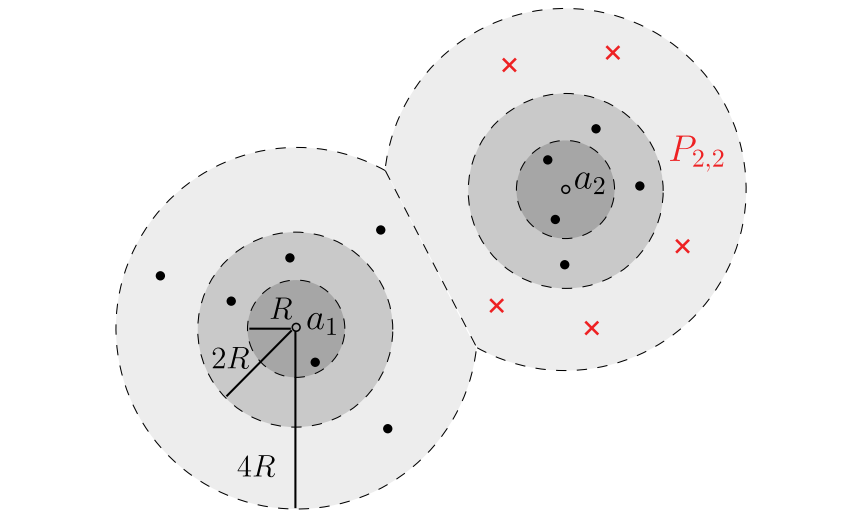
\includegraphics[width=0.4\textwidth]{figure/balls.png}
    \caption{环状分区示意图（Ring Partitioning of $P$ with respect to center $a_i$）~\cite{chen2009coresets}}
    \label{fig:ring-sets}
\end{figure}

\begin{remark}
集合 $P_{i,j}$ 的计算方式如下：对于每个点 $p \in P$，我们首先计算
$\mathbf{d}(p, a_1), \dots, \mathbf{d}(p, a_m)$，
从而确定该点 $p$ 属于哪个 $P_i$。
接着，根据 $\mathbf{d}(p, a_i)$ 与 $R$，我们可以立即判断该点属于哪个 $P_{i,j}$：如果 $\mathbf{d}(p, a_i) \le R$，则令 $j = 0$；否则，令 
    $j = \left\lceil \log \frac{\mathbf{d}(p, a_i)}{R} \right\rceil$。
% \begin{itemize}
%     \item 如果 $\mathbf{d}(p, a_i) \le R$，则令 $j = 0$；
%     \item 否则，令 
%     $j = \left\lceil \log \frac{\mathbf{d}(p, a_i)}{R} \right\rceil$。
% \end{itemize}
对所有点执行这一过程的总时间复杂度为
$O(mn) = O(\alpha k n) = O(nk)$，
因为 $\alpha = O(1)$。
\end{remark}


% \noindent \textbf{Remark}: 集合 $P_{i,j}$ 的构造过程：



% 对于每个点 $p \in P$，首先计算其到所有中心的距离：
% \[
% \mathbf{d}(p, a_1),\ \mathbf{d}(p, a_2),\ \dots,\ \mathbf{d}(p, a_m)
% \]
% 由此可确定该点属于的最近中心 $a_i$ 及其对应的簇 $P_i$。接着，根据 $d(p, a_i)$ 与半径阈值 $R$ 的关系，可立即确定其所在的 ring 集合编号 $j$：
% \[
% j =
% \begin{cases}
% 0, & \text{若 } d(p, a_i) \leq R \\
% \left\lceil \log\left( \dfrac{d(p, a_i)}{R} \right) \right\rceil, & \text{若 } d(p, a_i) > R 
% \end{cases}
% \]
% 这一过程可在 $O(mn)$ 时间内完成。由于 $m \leq \alpha k$ 且 $\alpha = O(1)$，故总时间复杂度为 $O(\alpha kn) = O(nk)$。

\noindent \textbf{步骤二：随机抽样}

设采样大小为：
\begin{equation}
s = \left\lceil \frac{c \beta^2}{\varepsilon^2} \left( k \ln n + \ln \frac{1}{\lambda} \right) \right\rceil,
\end{equation}
其中 $c$ 是一个充分大的常数。

对于所有 $i = 1, \dots, m$ 和 $j = 0, \dots, \phi$，若 $|P_{i,j}| \leq s$，则直接令：
\[
\mathcal{S}_{i,j} = P_{i,j}.
\]
否则，从 $P_{i,j}$ 中以\textbf{有放回}的方式独立、均匀地随机采样 $s$ 个点，并为每个采样点赋予权重 $|P_{i,j}| / s$，从而构成加权集合 $\mathcal{S}_{i,j}$。我们假设 $|P_{i,j}| / s$ 为整数（可通过适当取整或补齐实现）。
最终，构造的核集 $\mathcal{S}$ 定义为：
\[
\mathcal{S} = \bigcup_{i,j} \mathcal{S}_{i,j}.
\]
我们称该集合 $\mathcal{S}$ 是点集 $P$ 的一个 $(k, \varepsilon)$-coreset。

\subsection{正确性证明}
\noindent \textbf{观察}  \quad 设 $P_{i,j}$、$A$、$R$、$\beta$、$n$ 和 $\nu_{\mathrm{opt}}$ 的含义与前文相同，则有：
\begin{enumerate}
    \item 对于每个 $p \in P_{i,0}$，有 $0 \leq \mathbf{d}(A, p) \leq R$。
    \item 对于每个 $p \in P_{i,j}$，其中 $j \geq 1$，有 $2^{j-1}R < \mathbf{d}(A, p) \leq 2^j R$。
    \item $\beta n R = \nu(A, P) \leq \beta \nu_{\mathrm{opt}}$，其中 $\nu_{\mathrm{opt}} = \nu_{\mathrm{opt}}(k, P)$。
\end{enumerate}

\begin{claim}
\label{claim:3.4-cn} 设 $\nu_{\mathrm{opt}} = \nu_{\mathrm{opt}}(k, P)$。则有 $\sum_{i,j} |P_{i,j}|\, 2^j R \leq 3\nu(A, P) \leq 3\beta \nu_{\mathrm{opt}}$ 以及 $\sum_{i,j} |P_{i,j}|\, \mathrm{diam}(P_{i,j}) \leq 6\nu(A, P) \leq 6\beta \nu_{\mathrm{opt}}$ 成立。
% \[
% \sum_{i,j} |P_{i,j}|\, 2^j R \leq 3\nu(A, P) \leq 3\beta \nu_{\mathrm{opt}},
% \quad \text{以及} \quad
% \sum_{i,j} |P_{i,j}|\, \mathrm{diam}(P_{i,j}) \leq 6\nu(A, P) \leq 6\beta \nu_{\mathrm{opt}}。
% \]

\begin{proof}
设 $p$ 是 $P_{i,j}$ 中的任意一点。根据观察(1)，当 $j = 0$ 时，$2^j R = R$；当 $j \geq 1$ 时，有 $2^j R \leq 2\mathbf{d}(A, p) + R$。因此，
\[
2^j R \leq \max\bigl(2\mathbf{d}(A, p),\, R \bigr) \leq 2\mathbf{d}(A, p) + R\mathcnperiod
\]
于是
\begin{align*}
\sum_{i,j} |P_{i,j}|\, 2^j R
&= \sum_{i,j} \sum_{p \in P_{i,j}} 2^j R \\
&\leq \sum_{i,j} \sum_{p \in P_{i,j}} \bigl( 2\mathbf{d}(A, p) + R \bigr) \\
&= \sum_{p \in P} \bigl( 2\mathbf{d}(A, p) + R \bigr) \\
&= 2\nu(A, P) + |P| R \\
&= 2\nu(A, P) + nR \\
&\leq 3\nu(A, P) \leq 3\beta \nu_{\mathrm{opt}},
\end{align*}
其中最后一步使用了观察(3)。
另一方面，由于 $\mathrm{diam}(P_{i,j}) \leq 2(2^j R)$，上述不等式同时也推出了命题的第二部分。
\end{proof}
\end{claim}

\begin{lemma}(\cite[Lemma 3.5]{chen2009coresets})
\label{lem:3.5-cn}
对于所有满足 $|C| \leq k$ 的集合 $C \subseteq P$，有
\[
\bigl| \nu(C, P) - \nu(C, S) \bigr| \leq \varepsilon \, \nu(C, P)
\]
以至少 $1 - \lambda/2$ 的概率成立。
\end{lemma}

\begin{theorem}(\cite[Theorem 3.6]{chen2009coresets})
\label{thm:3.6-cn}
设 $P$ 是度量空间中的一个包含 $n$ 个点的集合，给定参数 $1 > \varepsilon > 0$ 和 $\lambda > 0$，则可以在 
$\mathcal{O}\bigl( nk \log(1/\lambda) \bigr)$
的时间内计算出一个带权集合 $S$，其大小满足
$|S| = \mathcal{O}\bigl( k \varepsilon^{-2} \bigl( k \log n + \log (1/\lambda) \bigr) \log n \bigr)$，
并且 $S$ 是集合 $P$ 在 $k$-median 聚类意义下的一个 $(k, \varepsilon)$-coreset，成立的概率至少为 $1 - \lambda$。 如果点集 $P$ 是带权的，总权重为 $W$，则其运行时间为 
$O(nk \log(1/\lambda) \log \log W)$，而 coreset 的大小为 
$O(k\varepsilon^{-2}(k \log n + \log(1/\lambda)) \log^2 W)$。
\end{theorem}
\begin{proof}
该算法的具体步骤在第~\ref{sec:coreset-con}节中给出。假设 
$\nu(A, P) \leq \beta \nu_{\mathrm{opt}}(k, P)$
以至少 $1 - \lambda/2$ 的概率成立。由引理~\ref{lem:3.5-cn}，可知对于所有大小至多为 $k$ 的集合 $C \subseteq P$，有
\[
\bigl| \nu(C, P) - \nu(C, S) \bigr| \leq \varepsilon \nu(C, P)
\]
以至少 $1 - \lambda/2$ 的概率成立。将两者结合可得该性质以至少 $1 - \lambda/2 - \lambda/2 = 1 - \lambda$ 的概率成立。
如果 $P$ 是无权的（unweighted），则 coreset 的大小满足
\[
|S| = \mathcal{O}(m \phi_S) = \mathcal{O}\bigl(k \varepsilon^{-2} (k \log n + \log (1/\lambda)) \log n \bigr)\mathcnperiod
\]
如果 $P$ 是有权的（weighted），则
\[
|S| = \mathcal{O}(m \phi_S) 
= \mathcal{O}\bigl(k \varepsilon^{-2} (k \log n + \log (1/\lambda)) \log^2 W \bigr)\mathcnperiod
\]
算法的整体运行时间主要由计算集合 $A$ 的过程决定。当 $P$ 为无权时，运行时间为 
$\mathcal{O}\bigl( nk \log(1/\lambda) \bigr)$，
当 $P$ 为有权时，运行时间为 
$\mathcal{O}\bigl( nk \log(1/\lambda) \log \log W \bigr)$。
\end{proof}






% \noindent \textbf{分析}

% 固定 $\forall c=\{c_1, c_2, \dots, c_k\} \subseteq \mathbb{R}^{d}$, 定义距离函数 $g(p,c)=\min_{1 \leq i \leq k} \|p - c_i\|$, 对于$\forall p, p'\in P_{i,j}$有：
% \begin{equation*}
%     |g(p,c)-g(p',c)|\leq 2^{j+1}\cdot R
% \end{equation*}

% 利用Hoeffding Bound,在$P_{i,j}$中取$x=\Theta(\frac{1}{\epsilon_{0}^{2}}log\frac{1}{\lambda})$个点，以$1-\lambda$的概率有：
% \begin{equation*}
%     \left| \frac{1}{|S_{i,j}|} \sum_{p \in S_{i,j}} g(p, c) - \frac{1}{|P_{i,j}|} \sum_{p \in P_{i,j}} g(p, c) \right| \leq \varepsilon_0 \cdot 2^{j+1} R
% \end{equation*}
% 同时有：
% \begin{equation*}
%     \left|
% \sum_{i=1}^{m} \sum_{j=0}^{\phi} \sum_{p \in S_{i,j}} \frac{|P_{i,i}|}{x} g(p, c)
% -
% \sum_{j=1}^{m} \sum_{t=0}^{\phi} \sum_{p \in S_{i,j}}g(p', c)
% \right|
% \leq
% \sum_{i=1}^{m} \sum_{j=0}^{\phi} \varepsilon_0 \cdot 2^{j+1} R \cdot |P_{i,j}|\leq 4\epsilon_{0} \cdot \nu(\mathcal{A}, P)
% \end{equation*}
% for $j\geq 1$.

% \begin{theorem}
%     对于所有大小不超过 $k$ 的集合 $C \subseteq P$，有：
% \[
% |\nu(C, P) - \nu(C, S)| \leq \varepsilon \nu(C, P),
% \]
% 成立的概率至少为 $1 - m(\phi+1)\lambda$, $x=O(\frac{\alpha^2}{\epsilon^2} log\frac{klogn}{\lambda})$, 所以$|\mathcal{S}| =O(m\phi x )$。
% \end{theorem}

\noindent \textbf{Streaming性质：}
\begin{enumerate}

\item 如果 $\mathcal{S}_1$ 和 $\mathcal{S}_2$ 分别是两个互不相交的集合 $P_1$ 和 $P_2$ 的 $(k, \varepsilon)$-coreset，
则 $\mathcal{S}_1 \cup \mathcal{S}_2$ 是 $P_1 \cup P_2$ 的一个 $(k, \varepsilon)$-coreset。

\item 如果 $\mathcal{S}_1$ 是 $\mathcal{S}_2$ 的一个 $(k, \varepsilon)$-coreset，且 $\mathcal{S}_2$ 是 $\mathcal{S}_3$ 的一个 $(k, \delta)$-coreset，
则 $\mathcal{S}_1$ 是 $\mathcal{S}_3$ 的一个 $(k, (1+\varepsilon)(1+\delta)-1)$-coreset。

\end{enumerate}

% \noindent \textbf{Merge-Reduce Tree:}

% \begin{figure}[htbp]
%     \centering
%     \includegraphics[width=0.6\textwidth]{figs/output (1).png}
%     \caption{Merge-Reduce Tree}
%     \label{fig:Merge-Reduce Tree}
% \end{figure}

% \begin{enumerate}
%     \item 叶节点为 1 到 12，表示最底层的数据块。

% \item 节点 3, 6, 10, 13 分别合并子节点。

% \item 节点 7 和 14 进一步合并，最终合并为根节点 15。
% \end{enumerate}

% 主要应用于流数据更新Coreset.

\section{重要性采样（Importance Sampling）}

设 $\{q_1, q_2, \dots, q_n\} \subseteq [0, \Delta]$。根据 Hoeffding 不等式，若采用 \textbf{均匀采样}，为了保证以 $1 - \delta$ 的概率使误差不超过 $\varepsilon$，所需的样本数为
\begin{equation}
m = \mathcal{O}\left(\frac{\Delta^2}{\varepsilon^2} \log \frac{1}{\delta}\right)\mathcnperiod
\end{equation}
然而，当
\begin{equation}
\mu = \frac{1}{n} \sum_{i=1}^n q_i \ll \Delta
\end{equation}
时，均匀采样的效果往往较差。这是因为 Hoeffding 界依赖于 $\Delta$ 的上界，而与实际数据分布无关，导致所需样本数被过大估计。

为改善这一问题，可以引入 \textbf{重要性采样（Importance Sampling）}。该方法对所有数据点进行如下变换：
\begin{equation}
q_i \;\rightarrow\; \bar{q}_i = \frac{\phi}{n\,\phi_i} \cdot q_i,
\quad 0 \le \bar{q}_i \le \phi_i,
\quad \phi = \frac{1}{n} \sum_{i=1}^n \phi_i ,
\end{equation}
其中 $\phi_i$ 是与数据点 $i$ 相关的某个重要性权重。

接着，以如下概率对变换后的 $\bar{q}_i$ 进行采样：
\begin{equation}
\mathrm{Prob}(\bar{q}_i) = \frac{\phi_i}{\phi}\mathcnperiod
\end{equation}

该变换保持了期望不变：
\begin{align}
\sum_{i=1}^n \mathrm{Prob}(\bar{q}_i) \cdot \bar{q}_i
&= \sum_{i=1}^n \frac{\phi_i}{\phi} \cdot \frac{\phi}{n\,\phi_i} \cdot q_i \notag \\
&= \frac{1}{n} \sum_{i=1}^n q_i\mathcnperiod
\end{align}

同时，可以验证对于任意 $i$，有 $\bar{q}_i \in \left[0, \frac{\phi}{n}\right]$，而原始的 $q_i \in [0, \Delta]$。  
因此，再次应用 Hoeffding 不等式，可得在重要性采样下所需的样本数为
\begin{equation}
m = \mathcal{O}\left(\frac{\phi^2}{n^2 \varepsilon^2} \log \frac{1}{\delta}\right)\mathcnperiod
\end{equation}

与均匀采样相比，当 $\phi \ll n\Delta$ 时，重要性采样所需的样本数显著减少，从而在保证相同误差界的前提下，大幅降低了采样复杂度。关于利用重要性采样构建 coreset 的具体方法和算法，可参见文献~\cite{feldman2011unified}.

\section{深度学习中的 Coreset}

随着现代深度学习模型在规模日益庞大的数据集（如 ImageNet、OpenWebText 等）上进行训练，训练过程变得愈发昂贵且耗时，带来了严重的计算与存储开销。这种 \textbf{数据爆炸} 现象进一步加剧了 \textbf{效率瓶颈}：高昂的计算和内存成本限制了深度模型的可扩展性，尤其是在边缘设备或资源受限的场景下。为应对这一问题，\textbf{coreset} 方法被提出，其核心思想是从原始数据集中选取一个规模较小但具有代表性的数据子集，以尽可能保留原始训练过程中的模型行为。通过合理构建 coreset，可以在保证模型性能的前提下显著提升训练与推理的效率，减少存储和内存占用，并通过更优的数据选择提升泛化能力。然而，如何有效地选择既具有信息量又具备多样性的样本，使其能够准确反映数据分布与模型的学习动态，仍然是 coreset 方法面临的核心挑战。在本章节中，我们将主要介绍 \textbf{coreset} 在 \textbf{持续学习（Continual Learning）}、\textbf{主动学习（Active Learning）} 以及 \textbf{生成模型（Generative Models）} 中的应用。

\subsection{持续学习}

\emph{持续学习（Continual Learning）}是一种学习范式，其目标是在一系列连续到来的任务上对神经网络进行训练，使其能够在获取新知识的同时，保持在先前已学习任务上的性能。然而，该范式面临一个根本性的挑战，即 \textbf{灾难性遗忘（catastrophic forgetting）}：当模型适应新任务时，往往会导致其在早期任务上的性能显著下降。为缓解灾难性遗忘问题，\textbf{基于重放（replay-based）}的方法得到了广泛研究。这类方法通常维护一个小型的 \emph{记忆缓冲区（memory buffer）}，其中存储了部分历史训练样本。由于存储容量有限，核心问题在于如何有效地构建这一记忆缓冲区。一个自然的思路是从 \textbf{coreset} 的角度来处理该问题，即选取最具代表性的一小部分样本。形式化地，重放方法通常在固定大小为 $M$ 的记忆缓冲区约束下运行。对于每个 $t \geq 1$，设 $X_t$ 表示第 $t$ 个任务的数据，目标是从中选取一个 coreset $S_t \subseteq X_t$，使其能够很好地近似原始数据集 $X_t$。在训练新任务时，模型参数 $\theta$ 通过优化如下复合目标函数来更新，该目标同时考虑了当前任务数据与存储的 coreset：
\begin{equation}
\label{eq:continual-object-cn}
    L(\theta) = L(\theta; X_{t+1}) + \lambda L(\theta; M),
\end{equation}
其中 $\lambda > 0$ 控制重放项的权重。

\begin{example}
    为了解决上述灾难性遗忘问题，Yoon 等人~\cite{yoononline} 提出了 \textbf{Online Coreset Selection (OCS)} 方法。该方法简单而高效，在每一次迭代中选取最具代表性和信息量的样本，并以在线(Online)的方式在这些样本上训练模型。具体来说，他们提出了三种基于梯度的 coreset 选择准则：
\begin{enumerate}
    \item \textbf{小批量相似性（minibatch similarity）}：优先选择最能代表当前任务数据分布的样本；
    \begin{equation*}
        \mathcal{S}(b_{t,n} \mid \mathcal{B}_t) = 
\frac{ \nabla f_\Theta(b_{t,n}) \, \bar{\nabla} f_\Theta(\mathcal{B}_t)^\top }
{ \left\| \nabla f_\Theta(b_{t,n}) \right\| \cdot \left\| \bar{\nabla} f_\Theta(\mathcal{B}_t) \right\| }.
    \end{equation*}
    \item \textbf{样本多样性（sample diversity）}：鼓励选择冗余度较低的样本，以提高输入空间的覆盖率；
    \begin{equation*}
        \mathcal{V}(b_{t,n} \mid \mathcal{B}_t \setminus b_{t,n}) = 
\frac{-1}{N_t - 1} \sum_{p \ne n}^{N_t - 1} 
\frac{ \nabla f_\Theta(b_{t,n}) \, \nabla f_\Theta(b_{t,p})^\top }
{ \left\| \nabla f_\Theta(b_{t,n}) \right\| \cdot \left\| \nabla f_\Theta(b_{t,p}) \right\| }.
    \end{equation*}
    \item \textbf{Coreset 亲和性（coreset affinity）}：通过减少已选择样本与已获得知识之间的干扰，从而提升不同任务之间的稳定性。
    \begin{equation*}
        \mathcal{A}(b_{t,n} \mid \mathcal{B}_\mathcal{M} \sim \mathcal{M}) = 
\frac{ \nabla f_\Theta(b_{t,n}) \, \bar{\nabla} f_\Theta(\mathcal{B}_\mathcal{M})^\top }
{ \left\| \nabla f_\Theta(b_{t,n}) \right\| \cdot \left\| \bar{\nabla} f_\Theta(\mathcal{B}_\mathcal{M}) \right\| }.
    \end{equation*}
\end{enumerate}
其中，$b_{t,n} = \{x_{t,n}, y_{t,n}\}$ 表示第 $t$ 个任务中第 $n$ 个样本及其标签，$\mathcal{B}_t$ 表示当前任务的小批量样本集，$N_t$ 是 $\mathcal{B}_t$ 的大小，$\nabla f_\Theta(\cdot)$ 表示在参数 $\Theta$ 下计算得到的梯度，$B_M$ 表示从记忆缓冲区 $\mathcal{M}$ 中采样得到的样本集合。
\end{example}

\subsection{主动学习}
在本节中，我们主要介绍 \textbf{池式主动学习（pool-based active learning）}，这是深度学习中最常用的一类主动学习方法。池式主动学习假设最初只有一个较小的有标签数据集，以及一个较大的无标签数据池可供采样。它通常包含以下四个迭代步骤：  
\begin{enumerate}
    \item 在有标签数据集上训练目标模型；
    \item 基于训练好的模型，从无标签数据中选择重要样本；
    \item 将所选样本交由标注者进行标注； 
    \item 将新标注的数据添加回有标签数据集中。 
\end{enumerate}
在该过程中，通常会设定一个标注预算，其规模远小于无标签数据集的大小，因此只能在预算内标注少量重要样本。很自然地，可以从 \textbf{coreset 构建} 的角度来看待该问题。

\begin{example}
    Sener 和 Savarese~\cite{sener2018active} 将主动学习问题形式化为一个 \textbf{coreset 选择问题}，其核心思想是从无标签数据池中选择一个子集，使其在特征空间中能够很好地代表整个数据分布。具体地，他们将样本选择建模为一个 \emph{k-center} 问题：给定一个无标签样本池 $\mathcal{U}$ 和当前的有标签集合 $\mathcal{L}$，目标是选择一个大小为 $k$ 的子集 $\mathcal{S} \subseteq \mathcal{U}$，最小化所有样本点到其最近被选点的最大距离(如图~\ref{fig:enter-label1}所示)：
\begin{equation}
\label{eq:kcenter}
\min_{\mathcal{S} \subseteq \mathcal{U},\, |\mathcal{S}| = k} \; 
\max_{x \in \mathcal{U}} \; \min_{s \in \mathcal{S} \cup \mathcal{L}} \Delta(x, s),
\end{equation}
其中 $\Delta(\cdot, \cdot)$ 是在特征空间上的距离度量。该目标确保了所选样本集在输入空间中具有良好的覆盖性，从而提升模型在未标注区域的泛化能力。
\begin{figure}[H]
    \centering
    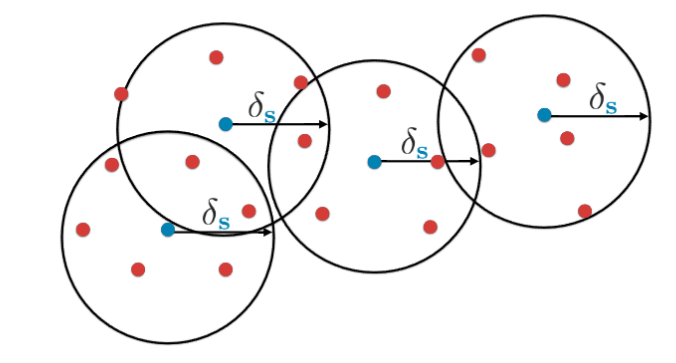
\includegraphics[width=0.5\linewidth]{figure/image.png}
    \caption{基于 k-center 的主动学习样本选择示意图。图中红点表示未标注样本，蓝点表示已选样本，圆表示以已选样本为中心的覆盖球，$\delta_s$ 表示未标注样本到最近已选样本的最大距离。该方法旨在最小化 $\delta_s$，从而最大化特征空间的覆盖。}
    \label{fig:enter-label1}
\end{figure}
\end{example}

\subsection{生成模型}
近年来，一些研究探索了如何利用 \textbf{coreset 选择} 来提升深度生成模型的训练效率。一类工作关注于 \textbf{数据子集选择}，即在训练前从完整数据集中选取一个小而具有代表性的子集用于模型训练。例如，Sinha 等人~\cite{sinha2020small} 提出通过选择信息量较大的样本子集来训练 GAN，并证明只使用原始数据的一小部分即可获得具有竞争力的生成效果。另一类研究则关注于 \textbf{自适应的 coreset 选择}，即在训练过程中根据样本对模型改进的贡献动态选择数据点，从而相比静态子集获得更好的数据利用效率。这些方法充分展示了 coreset 技术在降低深度生成模型的数据与计算需求方面的潜力，同时保持较高的模型性能。

\begin{example}
\label{ex:small-gan}
Small-GAN~\cite{sinha2020small} 通过引入两个 coreset 来提升 GAN 训练效率，其核心思想是将 coreset 选择问题形式化为一个 $k$-center 问题，并使用欧氏距离作为距离度量。具体来说，Small-GAN 分别在噪声分布和真实数据分布上构建两个 coreset：
\begin{itemize}
    \item \textbf{噪声分布 coreset}：从生成器输入的噪声分布中随机采样一个较大的批次，然后使用 Gonzalez 算法~\cite{gonzalez1985clustering} 选择一个较小的子集作为 coreset，用于生成多样化的样本。
    \item \textbf{真实数据 coreset}：首先计算真实样本的 Inception 嵌入表示（Inception Embeddings）~\cite{szegedy2017inception}，然后在嵌入空间中同样使用 $k$-center 选择，得到代表性的样本子集。
\end{itemize}
通过在噪声和真实数据上分别构建 coresets，Small-GAN 能够在不增加额外计算开销的情况下提升批次的代表性，从而稳定对抗训练过程并提升生成图像的质量。
\end{example}

\subsection{大语言模型中的 \textrm{Coreset}}

随着大语言模型（Large Language Models, LLMs）在自然语言处理任务中展现出卓越的能力，其训练所需的数据规模和计算成本也急剧上升。当前主流的 LLM 通常在万亿级别的文本数据上进行训练，这对存储、计算以及标注资源都提出了前所未有的挑战。如何在不显著降低模型性能的前提下，减少训练数据规模，已经成为大规模模型训练中的关键问题之一。 \textrm{Coreset} 技术为这一问题提供了一种有潜力的解决思路。通过从大规模数据集中选取一个具有代表性和信息性的子集进行训练，可以在大幅降低计算开销和存储需求的同时，保持甚至提升模型的泛化能力。在大语言模型的背景下，\textrm{Coreset} 主要应用于微调（fine-tuning）阶段的数据压缩与高效采样。

\begin{example}
\label{ex:colm}
Nguyen 等人（2025）~\cite{nguyen2025mini}提出了 \textbf{CoLM}（Coresets for Language Models）方法，将 coreset 技术应用于大规模语言模型的微调过程，以降低内存占用并提升训练效率。该方法的核心思想是：在每次迭代中，从一个较大的随机 mini-batch 中选择一个较小但能很好近似原始梯度的 \emph{mini-batch coreset}，从而在不损失模型性能的前提下减少激活缓存与梯度存储的开销。

与图像领域常用的梯度匹配方法不同，直接在语言数据上应用传统 coreset 方法效果较差，主要原因包括：（1）多数据源混合时存在显著的不平衡，小数据源样本容易被忽略；（2）Adam 优化器的梯度缩放影响未被考虑；（3）语言模型梯度空间维度极高，距离度量容易退化。为了解决这些问题，CoLM 提出了以下三步策略：
\begin{enumerate}
    \item \textbf{小数据源样本保留}：对来自小数据源的样本全部纳入 coreset，以保证它们在训练中的代表性；
    \item \textbf{梯度归一化}：对梯度进行历史归一化，使其更好地匹配 Adam 的自适应更新；
    \item \textbf{梯度维度压缩}：在最后的 V-projection 层上使用零阶梯度估计（SPSA）与梯度稀疏化技术，以降低维度并保留关键梯度信息。
\end{enumerate}

在多个主流模型（如 Phi-2、Phi-3、Zephyr、LLaMA-3）上的实验表明，CoLM 方法在仅使用一半 mini-batch 大小的情况下，就能达到甚至超过使用完整 batch 的训练效果，同时显著减少了 GPU 内存占用。这一结果展示了 coreset 技术在大规模语言模型训练中的强大潜力，尤其是在多数据源混合训练的场景下。
\end{example}


\printbibliography[heading=subbibliography, title={本章参考文献}]
\addcontentsline{toc}{section}{参考文献} % 手动添加到目录
\end{refsection}


\begin{refsection}
\chapter{最优传输}
% \section{Sinkhorn算法简介}
最优传输 (Optimal Transport, OT) 为比较概率分布提供了一个强大的几何工具~\cite{villani2008optimal}，在数据科学领域有着广泛的应用~\cite{peyre2019computational}。然而，对于大型数据集而言，精确OT的计算通常过于缓慢。本笔记介绍了Sinkhorn距离，它源于OT问题的熵正则化版本。熵正则化平滑了问题，使得通过Sinkhorn算法可以实现更快速的迭代求解。我们将探讨其公式、算法，并讨论为什么Sinkhorn距离已成为在实际大规模数据科学任务中应用OT原理的基石。


\section{最优传输 (OT) 简介}

\subsection{问题背景：搬土堆}
想象一下，你有两堆土，代表两个概率分布。最优传输，在其最初由Monge提出的形式中，旨在找到将第一堆土以最有效的方式移动以匹配第二堆土的形状，同时最小化所做的总功（例如，质量 $\times$ 距离）。

在数据科学中，这些“土堆”可以是直方图、词嵌入、图像像素强度或数据的任何其他离散表示。移动“土”的“成本”可以通过距离度量来定义（例如，特征向量之间的欧几里得距离）。

\subsection{数学公式 (Kantorovich松弛)}
令 $r \in \R_+^n$ 和 $c \in \R_+^m$ 为两个离散概率分布（直方图），即 $\sum_{i=1}^n r_i = \sum_{j=1}^m c_j = 1$。（原论文也考虑了非归一化的正向量，这是一个轻微的推广。）
令 $C \in \R_+^{n \times m}$ 为\textbf{成本矩阵}，其中 $C_{ij}$ 是将单位质量从分布 $r$ 的第 $i$ 个箱格运输到分布 $c$ 的第 $j$ 个箱格的成本。

目标是找到一个\textbf{传输计划}（或耦合）$P \in \R_+^{n \times m}$，它指定了从箱格 $r_i$ 到箱格 $c_j$ 流动多少质量 $P_{ij}$。该计划必须满足边际约束：
\begin{align}
    \sum_{j=1}^m P_{ij} &= r_i \quad \forall i=1, \dots, n \quad (P\mathbf{1}_m = r) \\
    \sum_{i=1}^n P_{ij} &= c_j \quad \forall j=1, \dots, m \quad (P^T\mathbf{1}_n = c)
\end{align}
所有此类有效传输计划的集合表示为 $U(r,c)$。

\textbf{最优传输距离}（或推土机距离、Wasserstein距离）是最小的总成本：
$$ L_C(r,c) = \min_{P \in U(r,c)} \sum_{i=1}^n \sum_{j=1}^m P_{ij} C_{ij} = \min_{P \in U(r,c)} \langle P, C \rangle_F $$
其中 $\langle \cdot, \cdot \rangle_F$ 是Frobenius内积。

% --- 图1占位符：OT图示 ---
\begin{figure}[!ht]
    \centering
     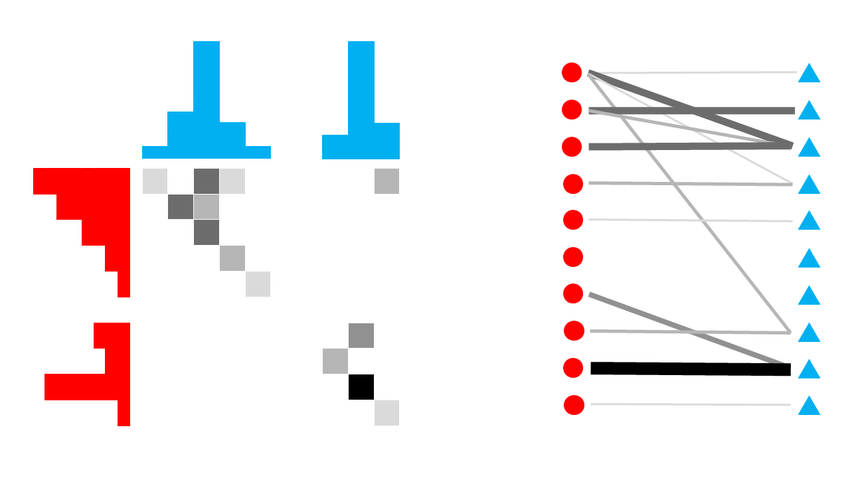
\includegraphics[width=0.9\textwidth]{figure/OT.png} % 取消注释并替换为您的图片
   % \fbox{\parbox{0.9\textwidth}{\centering \vspace{2cm} \textbf{图1占位符：} 展示两个分布 $r$ 和 $c$，一个成本矩阵 $C$，以及最优传输计划 $P$。 \vspace{2cm}}}
    \caption{最优传输概念示意图。左侧矩阵中的项对应两个分布的支撑点对应的coupling权重，颜色越深代表数值越大。右图是直观的匹配。}
    \label{fig:ot_concept}
\end{figure}
% --- 占位符结束 ---

\subsection{挑战：计算成本}
如上定义的OT问题是一个线性规划问题。对于具有 $n$ 和 $m$ 个箱格的分布，精确求解器复杂度约为 $O((n+m)^3 \log(n+m))$，如果 $n \approx m \approx N$，则为 $O(N^3 \log N)$。这对于大的 $N$（例如，$N > 1000$）来说计算成本过高，而这在许多数据科学应用中很常见（例如，高分辨率图像或大型词汇表~\cite{perrot2016mapping,yurochkin2019hierarchical}）。

\subsection{熵正则化：一条更平滑的路径}

为了克服计算障碍，可以在OT问题中添加\textbf{熵正则化}项的思想，从而引入矩阵缩放的算法以便加速和并行~\cite{peyre2019computational}。

\subsubsection{添加熵}
传输计划 $P$ 的熵定义为：
$$ H(P) = -\sum_{i,j} P_{ij} (\log P_{ij} - 1) $$
最大化熵鼓励传输计划 $P$ 更“平滑”或更分散，避免过于稀疏的解。

\subsubsection{正则化OT问题}
熵正则化OT问题为：
$$ L_C^\lambda(r,c) = \min_{P \in U(r,c)} \left( \sum_{i,j} P_{ij} C_{ij} - \lambda H(P) \right) $$
这里，$\lambda > 0$ 是\textbf{正则化参数}。
\begin{itemize}
    \item 当 $\lambda \to 0$ 时，问题接近原始（未正则化）的OT问题。
    \item 当 $\lambda \to \infty$ 时，熵项占主导地位，$P_{ij}$ 趋向于 $r_i c_j$（边际的乘积，忽略成本）。
    \item 对于有限的 $\lambda > 0$，我们得到一个权衡：一个计划 $P^\lambda$ 平衡了最小化真实传输成本和保持足够的熵。
\end{itemize}
关键的洞察是，这个正则化问题是严格凸的，并且可以更有效地求解。

%\textit{关于符号的说明：} Cuturi的论文中使用 $\lambda$ 作为正则化参数。我们这里使用 $\lambda$，这在文献中也很常见。成本矩阵在论文中通常表示为 $M$；我们使用 $C$。直方图在论文中是 $a, b$；我们使用 $r, c$。

\subsubsection{关于解空间的性质}
在讨论Sinkhorn算法之前，我们先引入两个与熵约束相关的引理。这里我们定义香农熵 (Shannon entropy) 为 $h(X) = -\sum_k X_k \log X_k$。注意这与上文定义的 $H(P)$ 略有不同：$H(P) = h(P) + \sum_{i,j} P_{ij}$。如果 $P$ 是一个概率分布 ($\sum P_{ij}=1$)，则 $H(P) = h(P)+1$。


\begin{lemma}
令 $U_\alpha(r,c) := \{P \in U(r,c) | KL(P || rc^T) \le \alpha\}$。则 $U_\alpha(r,c) = \{P \in U(r,c) | h(P) \ge h(r) + h(c) - \alpha\}$，并且 $U_\alpha(r,c) \subset U(r,c)$。
\end{lemma}
\begin{proof}
KL散度定义为 $KL(P || Q) = \sum_{i,j} P_{ij} \log \frac{P_{ij}}{Q_{ij}}$。
令 $Q_{ij} = r_i c_j$。则 $rc^T$ 表示 $r$ 和 $c$ 的独立耦合。
\begin{align*}
    KL(P || rc^T) &= \sum_{i,j} P_{ij} \log \frac{P_{ij}}{r_i c_j} \\
    &= \sum_{i,j} P_{ij} \log P_{ij} - \sum_{i,j} P_{ij} \log r_i - \sum_{i,j} P_{ij} \log c_j \\
    &= -h(P) - \sum_i \left(\sum_j P_{ij}\right) \log r_i - \sum_j \left(\sum_i P_{ij}\right) \log c_j
\end{align*}
由于 $P \in U(r,c)$，我们有 $\sum_j P_{ij} = r_i$ 和 $\sum_i P_{ij} = c_j$。代入上式：
\begin{align*}
    KL(P || rc^T) &= -h(P) - \sum_i r_i \log r_i - \sum_j c_j \log c_j \\
    &= -h(P) + h(r) + h(c)
\end{align*}
因此，条件 $KL(P || rc^T) \le \alpha$ 等价于 $-h(P) + h(r) + h(c) \le \alpha$，即 $h(P) \ge h(r) + h(c) - \alpha$。
$U_\alpha(r,c) \subset U(r,c)$ 的关系由 $U_\alpha(r,c)$ 的定义直接得出，因为它是在 $U(r,c)$ 的基础上增加了一个额外的约束。
\end{proof}

\begin{lemma}
集合 $U_\alpha(r,c)$ 是凸集。
\end{lemma}
\begin{proof}
首先，集合 $U(r,c) = \{ P \in \R_+^{n \times m} | P\mathbf{1}_m = r, P^T\mathbf{1}_n = c \}$ 是凸集。这是因为它是由一系列线性等式约束 ($P\mathbf{1}_m = r, P^T\mathbf{1}_n = c$) 和非负约束 ($P_{ij} \ge 0$) 定义的，这些约束共同形成一个多面体，因此是凸的。

其次，函数 $f(P) = KL(P || rc^T)$ 对于固定的 $rc^T$ 是关于 $P$ 的凸函数。
因此，集合 $\{P \in \R_+^{n \times m} | KL(P || rc^T) \le \alpha\}$ 是一个凸函数的子水平集 (sublevel set)，所以它也是凸集。

集合 $U_\alpha(r,c)$ 是两个凸集 $U(r,c)$ 和 $\{P | KL(P || rc^T) \le \alpha\}$ 的交集。两个凸集的交集仍然是凸集。
因此，$U_\alpha(r,c)$ 是凸集。
\end{proof}


\begin{theorem}\label{theo:metric} 对任意 $\alpha\geq 0$, $M\in\Mcal$, $d_{M,\alpha}$ 都对称且满足三角不等式。 %The function $(r,c)\mapsto \ones_{r\ne c} d_{M,\alpha}(r,c)$ satisfies all three distance axioms. 
\end{theorem}
%The gluing lemma~\cite[Lemma 7.6]{villani} plays a crucial role to prove that optimal transportation distances are indeed distances. The version we use below is slightly different since it incorporates the entropic constraint.
\begin{lemma}[熵约束下的粘合引理]\label{lem:gluing}
设 $\alpha\geq 0$，$x,y,z$ 为 $\Sigma_d$ 中的三个元素, $P\in U_\alpha(x,y)$ 和 $Q\in U_\alpha(y,z)$ 分别为 $(x,y)$ 和 $(y,z)$ 对应传输多面体中满足熵约束的两个联合概率分布, $S$ 为 $d\times d$ 矩阵，其第 $(i,k)$ 个元素定义为 $s_{ik}= \sum_{j} \frac{p_{ij}q_{jk}}{y_j}$。
则有 $S\in U_{\alpha}(x,z)$。
\end{lemma}
证明见Cuturi原文~\cite{cuturi13}。% We can prove the triangle inequality for $d_{M,\alpha}$ by using the same proof strategy than that used for classical transportation distances.

\begin{proof}[定理\ref{theo:metric}的证明]
$d_{M,\alpha}$ 的对称性源于$M$的对称性.设 $x,y,z\in\Sigma_d$. 设 $P\in U_{\alpha}(x,y)$和$Q\in U_{\alpha}(y,z)$为分别计算 $d_{M,\alpha}(x,y)$ 和$d_{M,\alpha}(y,z)$ 得到的最优解. 使用   引理\ref{lem:gluing}得到的$S$ of $U_{\alpha}(x,z)$, 我们有如下的不等式:
	$$\begin{aligned}
	d_{M,\alpha}(x,z)&=\min_{P\in U_\alpha(x,z)}\dotprod{P}{M} \leq \dotprod{S}{M} = \sum_{ik} m_{ik}\sum_{j} \frac{p_{ij}q_{jk}}{y_j} \\ & \leq \sum_{ijk} \left(m_{ij}+m_{jk}\right) \frac{p_{ij}q_{jk}}{y_j} = \sum_{ijk} m_{ij} \frac{p_{ij}q_{jk}}{y_j} +m_{jk} \frac{p_{ij}q_{jk}}{y_j}  \\
	& =\sum_{ij} m_{ij}p_{ij} \sum_k \frac{q_{jk}}{y_j} + \sum_{jk} m_{jk} q_{jk} \sum_i \frac{p_{ij}}{y_j}\\
	&= \sum_{ij} m_{ij}p_{ij} + \sum_{jk} m_{jk} q_{jk} = d_{M,\alpha}(x,y)+d_{M,\alpha}(y,z).\,\blacksquare\end{aligned}
	$$
\end{proof}


\subsection{Sinkhorn算法}

熵正则化OT问题的解 $P^\lambda$ 具有特定结构：
$$ P^\lambda_{ij} = u_i K_{ij} v_j $$
其中：
\begin{itemize}
    \item $K$ 是一个Gibbs核矩阵，其中 $K_{ij} = e^{-C_{ij}/\lambda}$。
    \item $u \in \R_+^n$ 和 $v \in \R_+^m$ 是缩放向量（对偶变量）。
\end{itemize}
这些缩放向量 $u$ 和 $v$ 可以通过一个称为\textbf{Sinkhorn算法}（或Sinkhorn-Knopp算法，最初为矩阵缩放开发）的简单迭代过程找到。

\subsubsection{迭代缩放}
给定 $r, c, C$ 和 $\lambda$：
\begin{enumerate}
    \item 计算 $K_{ij} = e^{-C_{ij}/\lambda}$。
    \item 初始化 $v^{(0)} = \mathbf{1}_m$（长度为 $m$ 的全1向量）。
    \item 对于 $l = 0, 1, 2, \dots$ 直到收敛：
    \begin{align}
        u^{(l+1)} &= r ./ (K v^{(l)}) \quad \text{(逐元素除法)} \\
        v^{(l+1)} &= c ./ (K^T u^{(l+1)}) \quad \text{(逐元素除法)}
    \end{align}
    （这里，$./$ 表示逐元素除法。为了数值稳定性，通常会向分母添加小常数，或在对数空间中进行计算。）
\end{enumerate}
一旦 $u$ 和 $v$ 收敛（例如，到 $u^*$ 和 $v^*$），最优正则化传输计划为 $P^\lambda = diag(u^*) K diag(v^*)$。

\begin{figure}
    \centering
    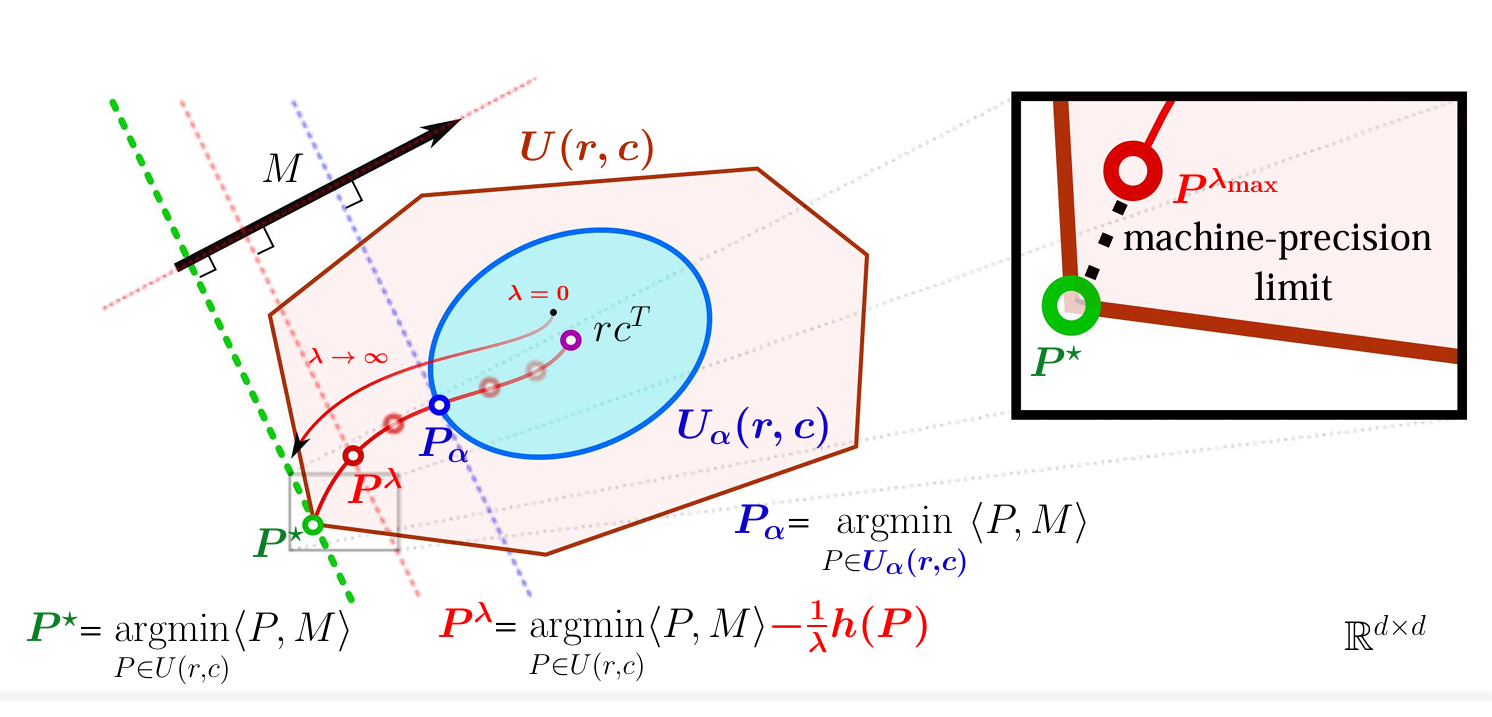
\includegraphics[width=0.9\linewidth]{figure/Sinkhorn.png}
    \caption{Sinkhorn算法的迭代过程。可以看到，对于固定的$\lambda$,$U_\alpha(r,c)$平滑地逼近原线性规划问题的凸多面体定义域。随着$\lambda$变大，Sinkhorn算法求得的解越来越趋近于最优传输问题的精确解。图源为\cite{cuturi13}}.
    \label{fig:enter-label2}
\end{figure}

\subsubsection{计算优势}
Sinkhorn算法的每次迭代都涉及矩阵-向量乘法（$K v$ 和 $K^T u$），其成本为 $O(nm)$。该算法通常收敛非常快（几何级数收敛）。与精确OT求解器的 $O(N^3 \log N)$ 复杂度相比，这是一个巨大的速度提升，使其对于数千甚至更大的 $N$ 都是可行的。

% --- 图2占位符：Sinkhorn迭代 ---
% \begin{figure}[h!]
%     \centering
%     % \includegraphics[width=0.7\textwidth]{your_sinkhorn_figure_zh.png} % 取消注释并替换为您的图片
%     \fbox{\parbox{0.9\textwidth}{\centering \vspace{2cm} \textbf{图2占位符：} 展示 $u$ 和 $v$ 的迭代更新以及 $P$ 如何演变，或显示收敛图。 \vspace{2cm}}}
%     \caption{Sinkhorn算法迭代的概念示意图。}
%     \label{fig:sinkhorn_iterations}
% \end{figure}
% --- 占位符结束 ---

\subsection{Sinkhorn距离}

从熵正则化问题的解中获得的 $L_C^\lambda(r,c)$ 的传输成本部分 $\langle P^\lambda, C \rangle_F$ 通常被称为\textbf{Sinkhorn距离}。
$$ d_{C,\lambda}(r,c) = \sum_{i,j} P^\lambda_{ij} C_{ij} $$
值得注意的是：
\begin{itemize}
    \item Sinkhorn距离是真实OT距离 $L_C(r,c)$ 的一个近似。正则化目标函数值 $L_C^\lambda(r,c)$ 是真实OT成本 $L_C(r,c)$ 的一个下界（如果 $\lambda H(P)$ 如目标函数中那样被减去）。更准确地说，$L_C^\lambda(r,c)$ 是正则化目标的值，而Sinkhorn距离本身是 $\langle P^\lambda, C \rangle_F$。对于 $\lambda > 0$，这个值通常大于 $L_C(r,c)$。
    \item 近似的质量取决于 $\lambda$。较小的 $\lambda$ 给出更接近的近似，但可能需要更多迭代并且可能存在数值不稳定性。较大的 $\lambda$ 导致更快的收敛和更稳定的计算，但是一个更粗糙的近似（一个更“模糊”的传输计划）。
\end{itemize}
% 尽管是近似值，但如果在 $C$ 的某些条件下考虑对偶目标值，Sinkhorn距离是真正的距离（它们满足度量属性），或者它们为许多实际目的提供了有用的散度。

% \section{为什么Sinkhorn距离对数据科学意义重大}

% 通过熵正则化引入Sinkhorn距离具有变革性的原因有几个：

% \subsection{使OT能够应用于大型数据集}
% 主要的好处是计算速度。数据科学家现在可以将类OT比较应用于：
% \begin{itemize}
%     \item 高维直方图（例如，在计算机视觉中）。
%     \item 大量文档集合（例如，词移距离 (Word Mover's Distance)，它使用OT根据词嵌入比较文档）。
%     \item 比较深度学习模型的嵌入。
% \end{itemize}

% \subsection{可微性}
% Sinkhorn算法的迭代对于其输入（成本矩阵 $C$，分布 $r, c$ 和 $\lambda$）是可微的。这使得Sinkhorn距离可以作为损失函数合并到深度学习流程中，并通过梯度下降进行优化。这对于像Wasserstein GAN（尽管通常使用不同的正则化或对偶公式）和其他生成模型等应用至关重要。

% \subsection{应用}
% Sinkhorn距离及其基础算法已得到广泛应用的一些领域：
% \begin{itemize}
%     \item \textbf{计算机视觉：} 图像检索、形状匹配、颜色转移、域自适应。
%     \item \textbf{自然语言处理：} 测量文档之间的相似性（词移距离）、比较句子嵌入。
%     \item \textbf{机器学习：} 生成对抗网络 (GAN)、域自适应、聚类、降维。
%     \item \textbf{生物学和图形学：} 对齐点云、比较细胞群体。
% \end{itemize}

% % --- 图3占位符：应用 ---
% \begin{figure}[h!]
%     \centering
%     % \includegraphics[width=0.8\textwidth]{your_applications_figure_zh.png} % 取消注释并替换为您的图片
%     \fbox{\parbox{0.9\textwidth}{\centering \vspace{2cm} \textbf{图3占位符：} 展示应用示例，例如图像颜色转移、文档相似性或域自适应。 \vspace{2cm}}}
%     \caption{受益于Sinkhorn距离的数据科学应用示例。}
%     \label{fig:applications}
% \end{figure}
% % --- 占位符结束 ---

% \section{结论}
% 最优传输问题的熵正则化，引出了Sinkhorn算法和Sinkhorn距离，代表了一项关键进展。它将OT从一个理论上优雅但通常计算成本过高的工具转变为数据科学家实用且可扩展的方法。通过接受一个轻微的近似（由正则化参数 $\lambda$ 控制），我们获得了巨大的计算速度提升，为在各种大规模数据上利用OT的几何洞察力的应用打开了大门。

% \section{进一步阅读}
% \begin{itemize}
%     \item Cuturi, M. (2013). Sinkhorn Distances: Lightspeed Computation of Optimal Transport Distances. In \textit{Advances in Neural Information Processing Systems 26} (NIPS 2013). (可查阅: \href{https://arxiv.org/abs/1306.0895}{arXiv:1306.0895})
%     \item Peyré, G., \& Cuturi, M. (2019). Computational Optimal Transport: With Applications to Data Science. \textit{Foundations and Trends® in Machine Learning, 11}(5-6), 355-607. (关于该主题的一本综合性书籍)。
% \end{itemize}


\section{最优传输的更多应用}
概率分布是统计和机器的核心对象。许多基本的机器学习问题，例如生成模型(generative modeling)和领域自适应(domain adaption)，可以统一地看作是找到一个传输映射来将一个分布转移到另一个分布。
\subsection{生成模型}
生成模型可以看成是如下的任务：
 \begin{problem}
       给定两个概率分布 $\pi_0, \pi_1$ on $\mathbb{R}^d$的采样集合，找到一个传输映射 $T\colon\mathbb{R}^d\to\mathbb{R}^d$， 使得在$Z_0 \sim \pi_0$时， $Z_1 := T(Z_0)\sim \pi_1$。 换句话说，$(Z_0,Z_1)$ 是$\pi_0$ 和 $\pi_1$之间的coupling或传输方案.
    \end{problem}
生成模型的常见类型根据问题已知的信息可以分成如下两类：
    \begin{enumerate}
    \item \textbf{生成}：这是指当 $\pi_1$ 是一个\textbf{经验观察得到的未知分布}（例如图像分布），而 $\pi_0$ 是一个基本分布，例如标准高斯分布时的情形。我们的目标是寻找一个非线性变换，使得从 $\pi_0$ 中采样的点可以被映射为服从数据分布 $\pi_1$ 的点。

    \item \textbf{迁移}：这是指当\textbf{$\pi_0$ 和 $\pi_1$ 都是经验观察得到的未知分布}时的情形，我们希望构建一个过程，将来自 $\pi_0$ 的数据点迁移为服从 $\pi_1$ 的点，或者反之。该任务具有广泛的应用，例如迁移学习中的领域自适应、图像编辑，以及机器人中的仿真到现实（sim2real）转换。
\end{enumerate}

 \begin{figure}\label{fig:rec}
        \centering
        \includegraphics[width=0.9\linewidth]{figure/transfer.png}
        \caption{上两行为生成任务，下两行为迁移任务。图源为\cite{liuflow}.}
        \label{fig:enter-label3}
    \end{figure}

既然涉及到了匹配问题，最优传输很自然地给出了一种匹配方案。对于任意两个概率分布之间的匹配，\cite{benamou2000computational}将 Wasserstein-2 距离重新表述为一个流体力学问题：

\begin{equation}\label{eq:BB}
{W_2^2(\mu_0, \mu_1) = \inf_{(\rho, v)} \int_0^1 \int_{\mathbb{R}^d} \rho_t(x) \|v_t(x)\|^2 \, dx \, dt}
\end{equation}

\noindent 约束条件为：

\begin{equation}\label{eq:continue}
\partial_t \rho_t + \nabla \cdot (\rho_t v_t) = 0, \quad \rho_0 = \mu_0, \quad \rho_1 = \mu_1
\end{equation}

\noindent 其中 $\rho_t$ 表示时间 $t$ 的密度，$v_t$ 表示速度场。式~\eqref{eq:continue} 被称为连续性方程。该表述具有很多优势：

\begin{enumerate}
    \item 它提供了源分布与目标分布之间的连续\textbf{插值}（可作为生成模型的训练对象）；
    \item 它与流体力学和偏微分方程（PDE）有紧密联系；
    \item 它可以推广以处理额外的约束或代价项（如Schrödinger桥\cite{de2021diffusion}）。
\end{enumerate}

当前最常见的图像生成模型为流匹配（flow matching）或其特例扩散模型（diffusion model），可以证明大多数训练方法在试图逼近动态最优传输的解\cite{liuflow,lipman2023flow}，或引入了最优传输作为匹配的指导准则\cite{tongimproving}.

\subsection{领域自适应}

领域自适应（domain adaption）的目标是在源领域上训练一个模型，并使其在一个不同但相关的目标领域上表现良好，其中标注数据可能有限甚至不可用。在实际应用中，训练数据与测试数据往往来自不同但相关的分布。例如，图像识别模型可能在清晰的实验室图像上训练，但需要在模糊的真实场景中部署。这种分布差异被称为“领域偏移”（domain shift）。领域自适应旨在解决这一问题：在源领域（source domain）上训练模型，并使其在目标领域（target domain）上保持良好性能，即使目标领域缺乏标注数据。



\begin{figure}
\centering
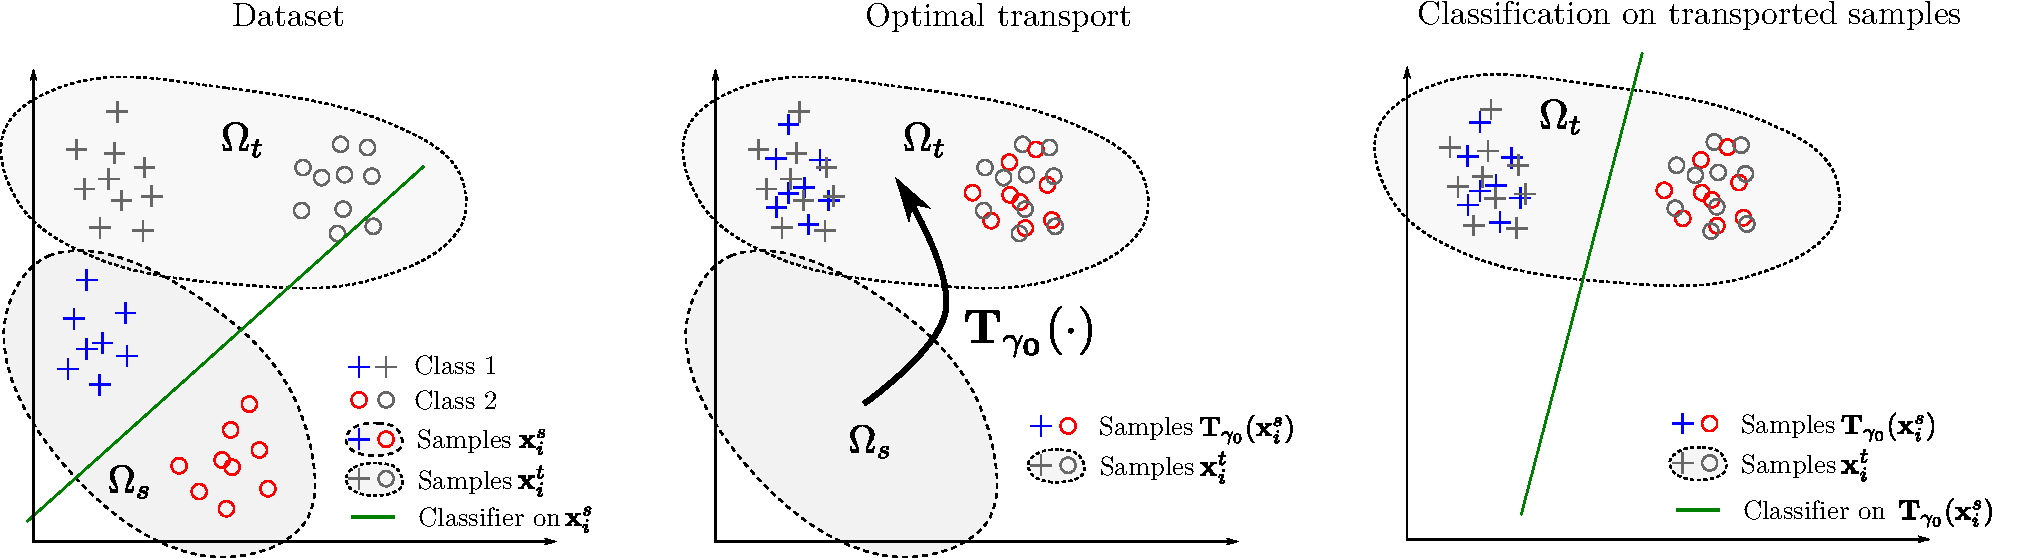
\includegraphics[width=1\linewidth]{figure/scheme.pdf}
\caption{最优传输（OT）在领域自适应中的示意图\cite{courty2016optimal}。（左）用于训练的数据集，即源领域，以及用于测试的数据集，即目标领域。注意：在训练样本上估计的分类器显然不适用于目标数据。（中）估计一个依赖数据的传输映射 $\mathbb{T}_{\gamma 0}$，用于将训练样本传输到目标领域。注意：这种变换通常是非线性的。（右）使用传输后的带标签样本在目标领域上估计分类器。}
\label{fig:illus_otda}
\end{figure}

为了解决领域适配问题：

\begin{enumerate}
\item 从源领域 $X_s$ 和目标领域 $X_t$ 的采样指标中估计分布 $\mu_s$ 和 $\mu_t$
\item 寻找一个传输映射 $\mathbf{T}$，将 $\mu_s$ 映射到 $\mu_t$
\item 使用 $\mathbf{T}$ 将带标签的样本 $X_s$ 传输到目标领域，并据此训练一个分类器
\end{enumerate}

事实上，这等同于寻找如下的最优传输映射：

\begin{equation}
{\mathbb{T}_0 = \argmin_\T  \int_{\Omega_s} c(\x,\T(\x))d\mu(\x), \;\;\;\;\; \text{使得：} \; \T_\#s=\mu_t}
\end{equation}

这里的 $T: \mathcal{X} \rightarrow \mathcal{Y}$为可测函数，$\mu \in \mathcal{P}(\mathcal{X})$为$X$上的概率测度, 前推测度 （pushforward measure）$T_{\#}\mu \in \mathcal{P}(\mathcal{Y})$ 被定义为:

\begin{equation}
{T_{\#}\mu(B) = \mu(T^{-1}(B))}
\end{equation}

上述形式成为Monge最优传输，容易看出$(Id\times T)_\# \mu_s$即为最优传输问题中的coupling。最优传输为领域自适应提供了一个理论完备、几何直观的框架\cite{courty2016optimal}。通过构造低代价的映射，我们可以在分布不一致的场景中实现有效的知识迁移。%未来的研究将进一步探索其在多模态、无监督和生成式任务中的潜力。

\subsection{Wasserstein分布鲁棒优化}


% \begin{abstract}
在现实世界的优化问题中，我们常常面临由未知概率分布驱动的不确定性。传统的随机规划（Stochastic Programming）依赖于对真实分布的精确了解，而样本平均近似（SAA）方法则容易对训练数据过拟合，导致样本外性能（out-of-sample performance）较差。分布式鲁棒优化（Distributional Robust Optimization, DRO）通过构建一个包含真实分布的“模糊集”（ambiguity set），并优化其在最坏情况分布下的性能，为这一问题提供了解决方案。本节介绍 Wasserstein 分布式鲁棒优化（WDRO），它利用 Wasserstein 距离（或称“推土机距离”）来构建模糊集。我们将探讨 WDRO 的基本形式、其强大的对偶重构（dual reformulation）技术，以及它为何能在提供鲁棒解的同时保持计算上的可处理性（tractability）。
% \end{abstract}

%------------------------------------------------
% \subsubsection{引言：不确定性下的优化}
%------------------------------------------------

许多优化问题（如投资组合管理、供应链设计、机器学习模型训练）的核心是处理不确定性。这些问题可以被抽象地表述为随机规划问题，其目标是最小化在某个概率分布 $P$ 下的期望损失：
\begin{equation}
\label{eq:sp}
\minimize_{\bx \in \Xcal} \quad \E_{P}[f(\bx, \bxi)]
\end{equation}
其中：
\begin{itemize}
    \item $\bx \in \Xcal \subseteq \R^d$ 是我们的决策变量。
    \item $\bxi \in \Zcal \subseteq \R^m$ 是一个受不确定性影响的随机向量（例如，未来的市场回报、客户需求）。
    \item $f(\bx, \bxi)$ 是损失函数（例如，负利润、预测误差）。
    \item $P$ 是 $\bxi$ 的真实但（通常）未知的概率分布。
\end{itemize}

% \subsubsubsection{样本平均近似 (SAA)}
由于 $P$ 是未知的，我们通常只有一组 $n$ 个独立同分布 (i.i.d.) 的数据样本 $\{\bxi_1, \dots, \bxi_n\}$。最常用的方法是样本平均近似（Sample Average Approximation, SAA），即用经验分布 $\Phat = \frac{1}{n} \sum_{i=1}^n \delta_{\bxi_i}$ 来代替 $P$：
\begin{equation}
\label{eq:saa}
\minimize_{\bx \in \Xcal} \quad \E_{\Phat}[f(\bx, \bxi)] = \minimize_{\bx \in \Xcal} \quad \frac{1}{n} \sum_{i=1}^n f(\bx, \bxi_i)
\end{equation}
SAA 在许多情况下（特别是 $n$ 很大时）是有效的。然而，它也存在严重缺陷：
\begin{itemize}
    \item \textbf{过拟合：} SAA 的解 $\bx^*$ 可能对训练样本 $\bxi_i$ 过度优化，导致其在“样本外”（即面对新数据时）表现不佳。
    \item \textbf{对异常值敏感：} 如果数据量 $n$ 相对于 $\bxi$ 的维度 $m$ 较小，或者数据中存在异常值，SAA 的解会非常不稳定。
\end{itemize}

% \subsubsection{分布式鲁棒优化 (DRO)}
为了克服 SAA 的局限性，分布式鲁棒优化 (Distributional Robust Optimization, DRO) 提出了一种更稳健的范式。DRO 不假定分布 $P$ 就是 $\Phat$，而是定义了一个“模糊集” $\Pcal$，该集合被认为以高概率包含了真实的分布 $P$。

DRO 的目标是寻找一个在 $\Pcal$ 中“最坏情况”分布下表现最好的决策 $\bx$，即求解一个 min-max 问题：
\begin{equation}
\label{eq:dro}
\minimize_{\bx \in \Xcal} \quad \sup_{\Q \in \Pcal} \quad \E_{\Q}[f(\bx, \bxi)]
\end{equation}
DRO 的鲁棒性和可计算性严重依赖于模糊集 $\Pcal$ 的选择。
那么，如何定义一个“好”的模糊集 $\Pcal$？
经典的模糊集包括基于矩的集合（例如，固定均值和协方差），但这类集合往往难以构建且可能导致计算困难。 另一类是基于概率散度（divergence）的，例如 $\phi$-散度（包括 $\chi^2$ 散度和 KL 散度）。例如，基于 KL 散度的集合：$\Pcal = \{ \Q \mid D_{KL}(\Q \| \Phat) \le \epsilon \}$。
然而，基于 KL 散度等 $\phi$-散度的模糊集在处理经验分布 $\Phat$（它是离散的）时存在一个重大问题：如果 $\Q$ 是一个连续分布，或者其支撑集与 $\Phat$ 不同，那么 $D_{KL}(\Q \| \Phat)$ 可能是无限大或未定义的。这使得模糊集 $\Pcal$ 变得非常受限。

% \subsubsection{Wasserstein 距离 (推土机距离)}
% Wasserstein 距离（又称 Optimal Transport 或 Earth-Mover's Distance）提供了一种更强大的方式来度量两个概率分布之间的“距离”。

% \begin{definition}[$p$-Wasserstein 距离]
% 设 $p \ge 1$，两个概率分布 $P_1$ 和 $P_2$（定义在 $\Zcal$ 上）之间的 $p$-Wasserstein 距离定义为：
% \begin{equation}
% W_p(P_1, P_2) = \left( \inf_{\pi \in \Pi(P_1, P_2)} \int_{\Zcal \times \Zcal} c(\mathbf{z}_1, \mathbf{z}_2)^p d\pi(\mathbf{z}_1, \mathbf{z}_2) \right)^{1/p}
% \end{equation}
% 其中：
% \begin{itemize}
%     \item $c(\mathbf{z}_1, \mathbf{z}_2)$ 是从 $\mathbf{z}_1$ 移动到 $\mathbf{z}_2$ 的“成本”，通常选择为 $c(\mathbf{z}_1, \mathbf{z}_2) = \|\mathbf{z}_1 - \mathbf{z}_2\|_q$（某个 $q$-范数）。
%     \item $\Pi(P_1, P_2)$ 是 $P_1$ 和 $P_2$ 的所有“联合分布”（或称“传输方案”）的集合，其边缘分布分别为 $P_1$ 和 $P_2$。
% \end{itemize}
% \end{definition}
% 直观地， $W_p(P_1, P_2)$ 是将分布 $P_1$ 的“质量”重新排列成分布 $P_2$ 所需的最小“成本”。

% \noindent
基于以上情况，可以使用 Wasserstein 距离定义模糊集，其优势在于：
\begin{enumerate}
    \item 它是一种真正的度量（metric），满足三角不等式。
    \item 即使两个分布的支撑集（support）不重叠，它也能给出有意义的距离（这是 KL 散度做不到的）。
    \item 它捕捉了 $\Zcal$ 空间中的几何结构，在高维空间中具有良好的统计性质。
\end{enumerate}

%------------------------------------------------
\subsubsection{Wasserstein DRO (WDRO) 的数学形式}
%------------------------------------------------

Wasserstein 分布式鲁棒优化 (WDRO) 使用 Wasserstein 距离来构建模糊集。具体来说，它定义了一个以经验分布 $\Phat$ 为中心、半径为 $\epsilon$ 的“Wasserstein 球”：
\begin{equation}
\label{eq:ambiguity_set}
\Pcal_\epsilon(\Phat) = \{ \Q \in \Pcal_0(\Zcal) \mid W_p(\Q, \Phat) \le \epsilon \}
\end{equation}
其中 $\Pcal_0(\Zcal)$ 是 $\Zcal$ 上所有概率分布的集合。

WDRO 问题就是求解在这个模糊集上的 min-max 问题：
\begin{equation}
\label{eq:wdro_minmax}
\boxed{
\minimize_{\bx \in \Xcal} \quad \sup_{\Q \in \Pcal_\epsilon(\Phat)} \E_{\Q}[f(\bx, \bxi)]
}
\end{equation}
这个问题的目标是找到一个决策 $\bx$，使得在距离经验分布 $\Phat$ 不超过 $\epsilon$ 的所有“最坏”分布 $\Q$ 下，期望损失 $\E_{\Q}[f(\bx, \bxi)]$ 也能被最小化。

%------------------------------------------------
% \section{对偶重构：从无穷维到有限维}
%------------------------------------------------

如何求解WDRO？注意到，式 \eqref{eq:wdro_minmax} 是一个无穷维的优化问题（因为它在所有可能的分布 $\Q$ 上进行了优化），这提升了优化难度。WDRO 成功的关键在于，其内部的 $\sup$ 问题通常具有一个可计算的、有限维的对偶形式。

\subsubsection{对偶结果}
WDRO 的核心理论是基于最优传输的强对偶定理。

\begin{theorem}[WDRO 对偶性\cite{kuhn2019wasserstein}]
对于 WDRO 内部的“最坏情况期望”问题（为简洁起见，设 $p=1$ 且成本 $c(\cdot, \cdot) = d(\cdot, \cdot)$）：
\begin{equation}
\label{eq:inner_sup}
\sup_{\Q : W_1(\Q, \Phat) \le \epsilon} \E_{\Q}[f(\bx, \bxi)]
\end{equation}
其对偶问题是一个有限维的最小化问题：
\begin{equation}
\label{eq:dual_inf}
= \inf_{\lambda \ge 0} \left\{ \lambda \epsilon + \E_{\Phat}\left[ \sup_{\mathbf{z} \in \Zcal} \{ f(\bx, \mathbf{z}) - \lambda d(\mathbf{z}, \bxi) \} \right] \right\}
\end{equation}
将 $\E_{\Phat}[\cdot] = \frac{1}{n} \sum_{i=1}^n [\cdot]_{\bxi = \bxi_i}$ 代入，上式变为：
\begin{equation}
\label{eq:dual_finite}
= \inf_{\lambda \ge 0} \left\{ \lambda \epsilon + \frac{1}{n} \sum_{i=1}^n \sup_{\mathbf{z} \in \Zcal} \left( f(\bx, \mathbf{z}) - \lambda d(\mathbf{z}, \bxi_i) \right) \right\}
\end{equation}
\end{theorem}

\noindent
\textbf{对偶形式的解释：}
\begin{itemize}
    \item $\lambda \ge 0$ 是对偶变量，可以被理解为对“鲁棒性” $\epsilon$ 的“惩罚价格”。
    \item $\sup_{\mathbf{z}} ( f(\bx, \mathbf{z}) - \lambda d(\mathbf{z}, \bxi_i) )$ 这一项非常关键。它寻找一个最坏的实现 $\mathbf{z}$，这个 $\mathbf{z}$ 使得损失 $f(\bx, \mathbf{z})$ 很大，但同时它又不能离数据点 $\bxi_i$ 太远（由 $d(\mathbf{z}, \bxi_i)$ 和惩罚 $\lambda$ 来平衡）。
\end{itemize}

% \subsection{可计算的重构问题}
将式 \eqref{eq:dual_finite} 的结果代回 WDRO 的 min-max 问题 \eqref{eq:wdro_minmax}，我们得到了一个等价的、可计算的最小化问题：
\begin{equation}
\label{eq:wdro_tractable}
\minimize_{\bx \in \Xcal, \lambda \ge 0} \quad \lambda \epsilon + \frac{1}{n} \sum_{i=1}^n \sup_{\mathbf{z} \in \Zcal} \left( f(\bx, \mathbf{z}) - \lambda d(\mathbf{z}, \bxi_i) \right)
\end{equation}

\noindent
这个问题的计算复杂度现在取决于内部的 $\sup_{\mathbf{z}}$ 问题。
\begin{itemize}
    \item \textbf{可计算性：} 在许多实际应用中（例如，当 $f(\bx, \mathbf{z})$ 对 $\mathbf{z}$ 是仿射的或凹的，且 $d(\cdot, \cdot)$ 是一个范数时），这个内部的 $\sup$ 问题可以被解析地（analytically）解出，或者可以被重构为标准的凸优化问题（如线性规划 LP、二阶锥规划 SOCP）。
    \item \textbf{凸性：} 如果原始损失 $f(\bx, \bxi)$ 对 $\bx$ 是凸的，那么重构后的问题 \eqref{eq:wdro_tractable} 通常也是关于 $(\bx, \lambda)$ 的凸优化问题，因此可以被高效求解。
\end{itemize}

%------------------------------------------------
% \section{理论保证与总结}
% %------------------------------------------------

% WDRO 框架不仅在计算上是可行的，而且在统计上也是有意义的。

% \subsection{统计保证}
% WDRO 最吸引人的地方之一是其模糊集半径 $\epsilon$ 的选择是数据驱动的。
% \begin{itemize}
%     \item \textbf{集中不等式 (Concentration Inequality):} 统计理论（特别是最优传输的集中不等式）告诉我们，经验分布 $\Phat$ 和真实分布 $P$ 之间的 Wasserstein 距离 $W_p(\Phat, P)$ 会随着 $n$ 的增加而收敛到 0。
%     \item \textbf{半径选择：} 我们可以选择 $\epsilon_n$，使其随着 $n$ 减小（例如，$\epsilon_n \sim n^{-1/m}$），从而保证真实分布 $P$ 以 $1-\beta$ 的高概率落在模糊集 $\Pcal_{\epsilon_n}(\Phat)$ 中。
%     \item \textbf{样本外性能 (Out-of-Sample Guarantee):} WDRO 的最优值 $V^*$（即 \eqref{eq:wdro_minmax} 的最优值）为真实分布下的期望损失提供了一个概率上界。这意味着 WDRO 的解 $\bx^*$ 具有可控的、高概率的样本外性能。
% \end{itemize}

% \subsection{总结}
% Wasserstein 分布式鲁棒优化 (WDRO) 是一个强大且灵活的框架，用于处理数据驱动优化中的不确定性。
% \begin{enumerate}
%     \item 它通过定义一个围绕经验分布的 Wasserstein 球来构建模糊集，克服了传统 $\phi$-散度（如 KL 散度）的局限性。
%     \item 它利用强大的对偶理论，将一个无穷维的 min-max 问题转化为一个有限维的（通常是凸的）优化问题，使其在计算上变得可行。
%     \item 它提供了强有力的样本外性能保证，其鲁棒性半径 $\epsilon$ 可以通过统计理论来合理选择。
% \end{enumerate}
% 由于这些优势，WDRO 已成为现代鲁棒优化和鲁棒机器学习（如鲁棒回归、鲁棒分类）领域中的一个核心工具。

\printbibliography[heading=subbibliography, title={本章参考文献}]
\addcontentsline{toc}{section}{参考文献} % 手动添加到目录
\end{refsection}
\begin{refsection}
\chapter{分布式算法}
\section{分布式算法综述}

\subsection{基础概念与研究动机}
\subsubsection{为什么需要分布式算法}
\textbf{计算能力瓶颈} \quad
摩尔定律曾预测芯片上晶体管数量每18–24个月翻倍，从而带来单机性能的快速提升。然而近年来这一趋势明显放缓：制程工艺接近物理极限（例如3nm以下制程面临量子隧穿问题），主频（GHz）自2010年前后基本停滞在4GHz左右，继续提升将导致功耗和散热成本急剧增加。因此，单核心性能提升变得越来越困难，计算机体系结构转向\textbf{多核并行}，但仍面临缓存一致性与带宽瓶颈的问题。

\textbf{存储与I/O瓶颈} \quad
即便CPU计算能力强大，如果\textbf{数据无法及时传输}，计算也无法高效进行。典型现象为“内存墙”（Memory Wall）：CPU性能增长速度远高于内存带宽增长，导致数据处理受限。此外，单机的磁盘、SSD、内存容量有限，在TB或PB级的大数据场景下，无法在一台机器上存放全部数据。

\textbf{扩展能力瓶颈} \quad
单机扩展（Scale-up）通过升级更高性能的CPU、内存、磁盘实现，但成本高昂且存在物理极限。相比之下，分布式扩展（Scale-out）通过多台廉价机器协同工作，更经济且易于扩展，是当前大规模计算的主流方向。

\subsubsection{通信复杂度}
在分布式计算中，\textbf{通信复杂度}是衡量算法性能的重要指标。其定义为不同计算节点之间传输的数据量。一个分布式算法的设计通常需要在计算复杂度与通信复杂度之间权衡。

\begin{itemize}
  \item \textbf{计算 vs. 通信}：在单机计算中，主要瓶颈通常是 CPU 计算能力；而在分布式计算中，节点计算速度很快，但如果频繁交换大量数据，网络延迟和带宽限制将极大影响整体性能。
  \item \textbf{典型例子}：在分布式机器学习训练中，如果每轮迭代都需要将完整的梯度矩阵发送到中心节点，那么通信开销将大大超过本地的矩阵乘法计算耗时，训练速度严重下降。
\end{itemize}

因此，一个核心问题是：\textbf{在分布式计算中，完成某个计算任务，最少需要多少通信量？} 这就是通信复杂度理论要解决的问题。
通信复杂度理论最早由姚期智（Andrew Yao）在 1979 年提出，是研究分布式计算中信息传递量的基础理论工具。

\begin{figure}[htbp]
    \centering
    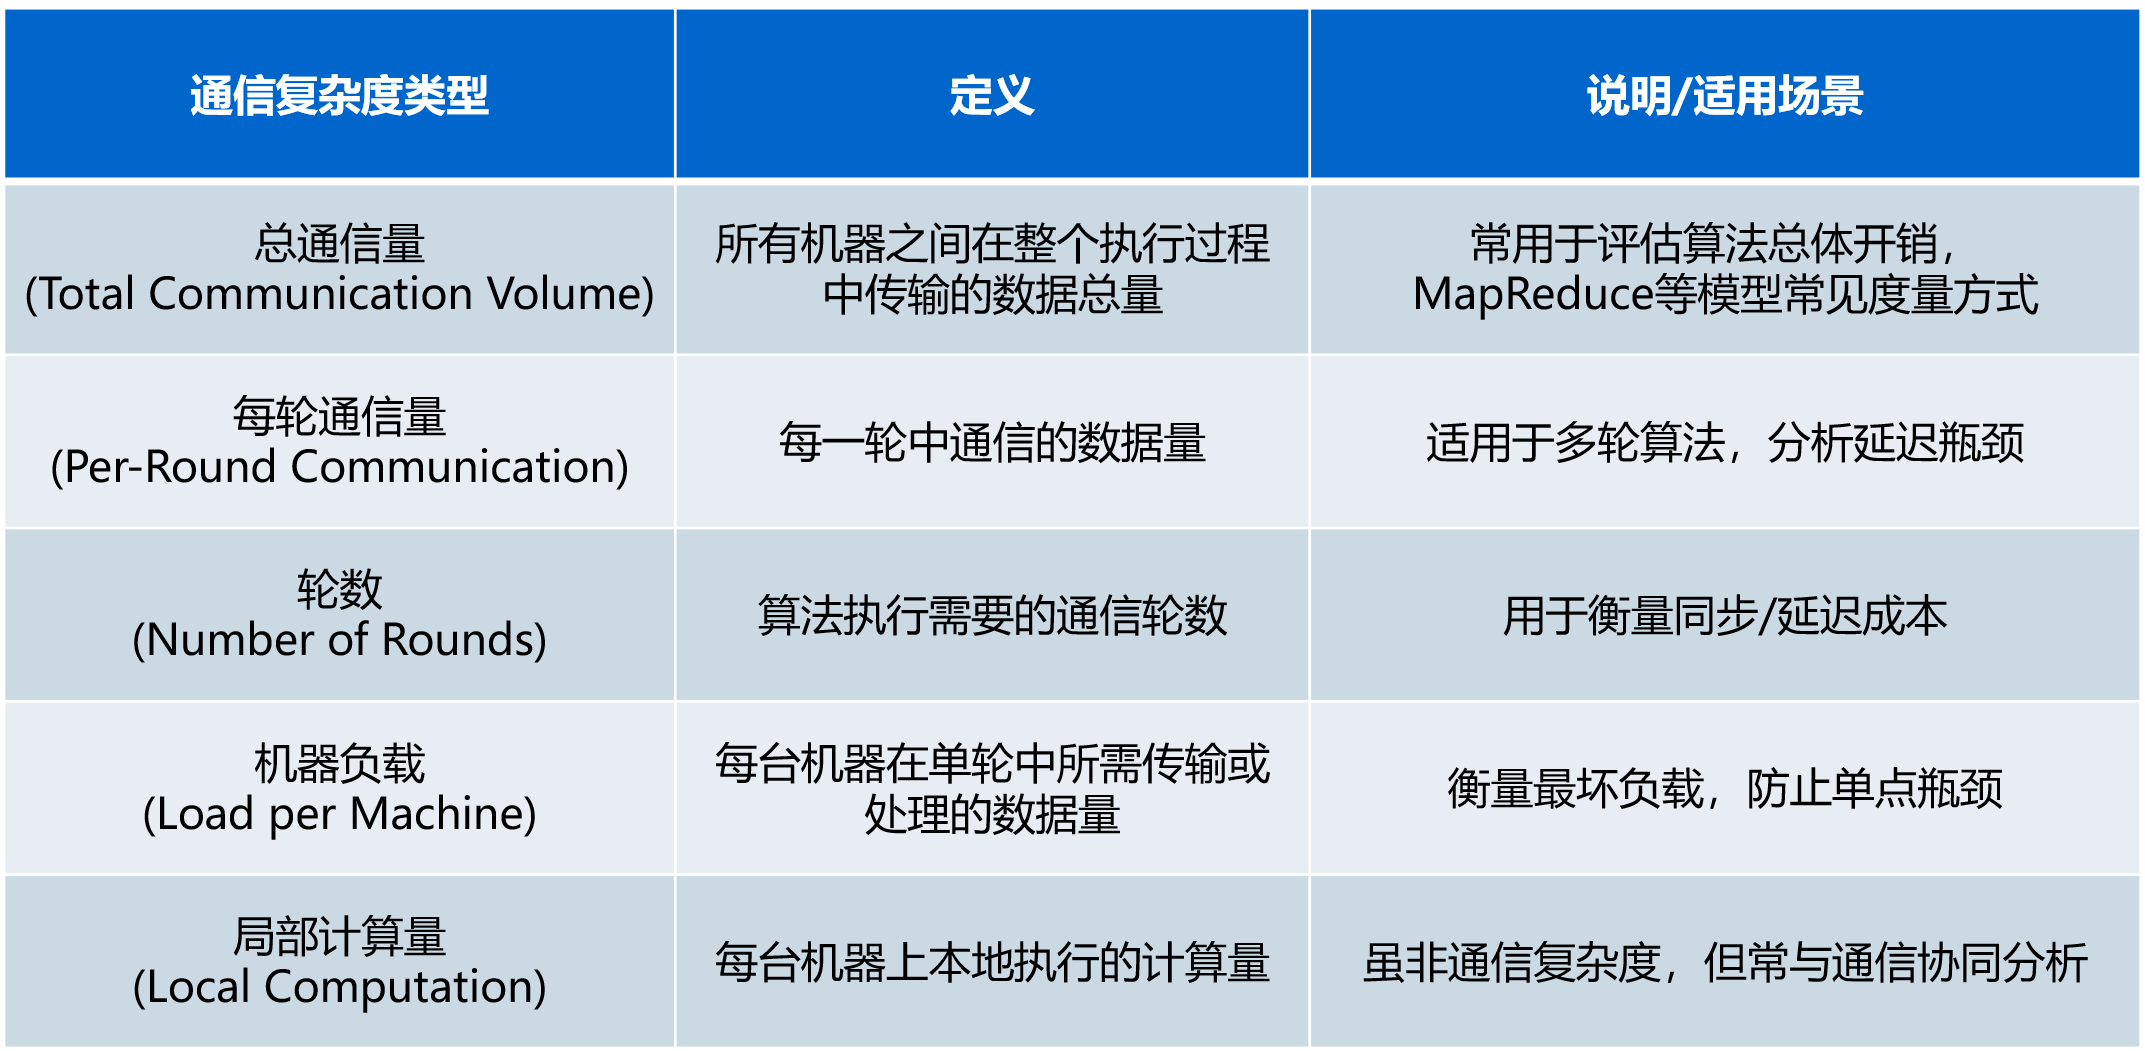
\includegraphics[width=0.8\linewidth]{figure/通信复杂度.png}
    \caption{各种通信复杂度类型之间的对比}
    \label{fig:communication}
\end{figure}

\subsubsection{分布式计算模型：MapReduce}
Google提出的MapReduce模型是分布式计算的经典框架，适用于TB甚至PB级数据的并行处理。其核心流程包括：
\begin{enumerate}
    \item \textbf{数据划分}：将输入数据拆分为多个块（split），分配给不同的Mapper节点；
    \item \textbf{Map阶段}：每个Mapper执行用户定义的Map函数，产生若干(key, value)对；
    \item \textbf{Shuffle阶段}：系统自动将相同key的数据发送到同一Reducer节点；
    \item \textbf{Reduce阶段}：Reducer对相同key的数据进行聚合处理；
    \item \textbf{结果输出}：输出结果存储到分布式文件系统（如HDFS）。
\end{enumerate}

\textbf{典型示例：分布式词频统计}

\begin{figure}[htbp]
    \centering
    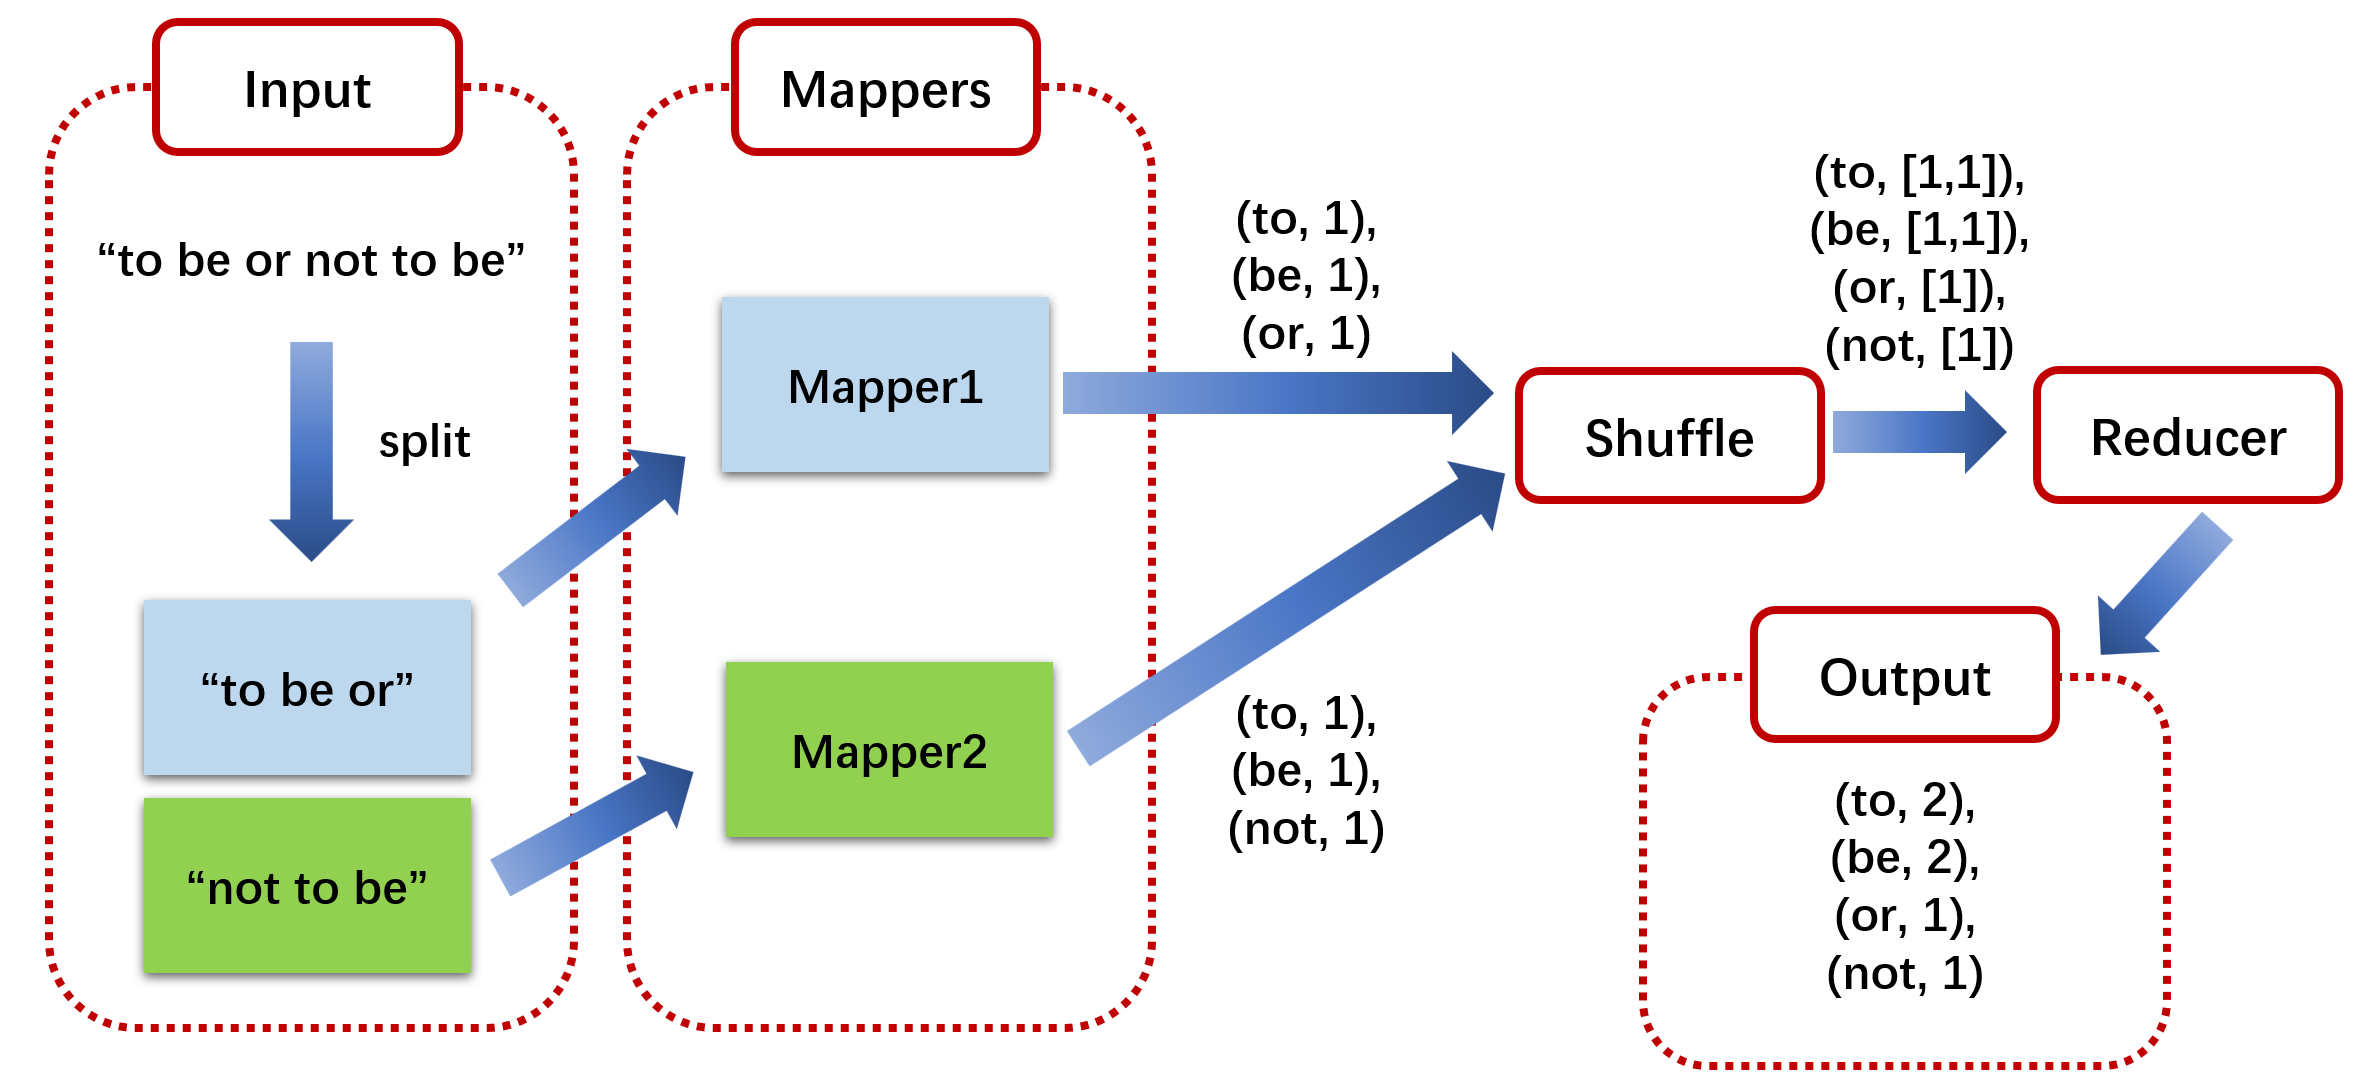
\includegraphics[width=0.8\linewidth]{figure/mapreduce.png}
    \caption{使用mapreduce进行词频统计的过程}
    \label{fig:mapreduce}
\end{figure}

本节通过一个经典的 ``词频统计（Word Count）'' 例子，来直观理解 MapReduce 的运行过程。假设我们有一批文本文件，目标是统计其中每个单词出现的次数。

\begin{enumerate}
    \item \textbf{数据划分}：系统首先将原始输入文本拆分为多个逻辑块（split）。例如，一段包含多行的文本被分为三块，分配给不同的 Mapper 节点，保证每个节点只处理自己负责的数据部分。
    
    \item \textbf{Map阶段}：每个 Mapper 节点读取其分配的数据块，并对文本进行处理。对于词频统计，Mapper 会将每一行文本拆分成单词，并输出 \texttt{(word, 1)} 形式的键值对，表示每出现一个单词就记一次。
    
    \item \textbf{Shuffle阶段}：系统自动将具有相同单词（key）的中间结果汇聚到同一个 Reducer 节点上。例如，所有关于 ``to'' 的 \texttt{(to, 1)} 会被送到同一个 Reducer。这一步是 MapReduce 框架的核心，它确保数据按照键进行全局分组。
    
    \item \textbf{Reduce阶段}：每个 Reducer 处理某一组相同键的值，将这些值进行聚合操作。对于词频统计，Reduce 过程就是对所有的 ``1'' 进行求和，得到该单词的总出现次数。
    
    \item \textbf{结果输出}：Reducer 输出的最终结果以 \texttt{(word, count)} 的形式写入分布式文件系统（如 HDFS），每个文件通常对应一个 Reducer 的输出。最后，所有输出文件合并即得到全局的词频统计结果。
\end{enumerate}

通过以上过程，MapReduce 将大规模的文本统计任务拆解为多个可并行执行的小任务，并在 Shuffle 阶段自动完成数据的全局分组，实现了高效、容错且可扩展的大数据处理。






\textbf{局限性}  
MapReduce并不适合迭代计算（如机器学习训练、图计算），其延迟较高，且中间结果频繁写入磁盘导致I/O开销大。后续出现了Spark、Flink等内存计算框架来弥补这些不足。

% -------------------- 第二章 分布式算法实现 --------------------
\subsection{典型分布式算法案例}

本节通过三个典型案例：分布式 $k$-center 聚类、分布式 PCA 降维、分布式 PageRank，介绍在大数据场景下如何将传统算法扩展到分布式环境中。核心思想都是通过\textbf{数据分区、局部计算、结果合并}来应对单机内存和计算资源不足的问题。

\subsubsection{分布式 \texorpdfstring{$k$}{k}-center 聚类}

$k$-center 聚类问题是聚类领域的经典问题之一，输入为一个点集 $P$ 和一个整数 $k$，目标是在 $P$ 中选择 $k$ 个中心，使得所有点到最近中心的最大距离最小化。这类问题在设施选址、内容分发网络优化、应急中心布局等领域都有广泛应用。然而在大规模数据场景中，传统的 $k$-center 算法面临以下挑战：数据量过大，单机内存无法容纳全部数据；中心选择需要全局距离计算，单机计算耗时巨大；同时数据往往分布在不同节点，通信成本成为主要瓶颈。

为了解决这些问题，可以将 $k$-center 算法改造成分布式版本，典型方法是在 MapReduce 框架下实现。具体过程如下：
\begin{enumerate}
    \item \textbf{Map阶段}：每个 Mapper 在本地数据块上运行 Gonzalez 贪心算法，选出一小部分候选中心；
    \item \textbf{Shuffle阶段}：系统将所有 Mapper 输出的候选中心发送到 Reducer；
    \item \textbf{Reduce阶段}：Reducer 再次运行 Gonzalez 算法，从候选中心中选出最终的 $k$ 个全局中心。
\end{enumerate}

在给出分布式版本之前，我们先回顾经典的 Gonzalez 贪心 $k$-center 算法~\cite{gonzalez1985clustering}，这是一个简单而重要的 $2$-近似算法。

\begin{algorithm}[htbp]
  \caption{Gonzalez  $k$-center 算法~\cite{gonzalez1985clustering}}
  \label{alg:gonzalez-seq}
  \renewcommand{\algorithmicrequire}{\textbf{Input:}}%
    \renewcommand{\algorithmicensure}{\textbf{Output:}}%
  \begin{algorithmic}[1]
    \Require 点集 $P$，簇数 $k$
    \Ensure 中心集合 $C \subseteq P$，$|C| = k$
    \State 任意选择一个点 $c_1 \in P$，令 $C \gets \{c_1\}$
    \For{$i = 2$ to $k$}
      \State 对每个点 $p \in P$， 计算其到当前中心集合$C$的距离
      \[
        d(p, C) = \min_{c \in C} d(p, c)
      \]
      \State 选择使 $d(p,C)$ 最大的点 $p^\star$：$p^\star = \arg\max_{p \in P} d(p, C)$
      \State 将 $p^\star$ 加入中心集合：$C \gets C \cup \{p^\star\}$
    \EndFor
    \State \Return $C$
  \end{algorithmic}
\end{algorithm}

\noindent
Gonzalez 算法的时间复杂度为 $O(nk)$，其中 $n = |P|$，因为每次选新中心要扫描所有点，并重复 $k$ 轮。记最优解的目标值（最小半径）为
\[
  \text{OPT}_k(P) = \min_{|C|=k} \max_{p \in P} d(p,C).
\]
可以证明，Algorithm~\ref{alg:gonzalez-seq} 输出的解 $C$ 满足
\[
  \max_{p \in P} d(p,C) \le 2 \cdot \text{OPT}_k(P),
\]
因此是一个 $2$-近似算法。证明思路是：任取最优中心集合 $C^\star$，考虑 Gonzalez 过程中两两选出的中心之间距离都不小于当前半径，再利用抽屉原理将这些中心映射到 $C^\star$ 中的 $k$ 个簇上，可以证明 Gonzalez 的半径至多是最优半径的两倍（详细证明可参考~\cite{gonzalez1985clustering}）。

在此基础上，可以设计一个只需两轮 MapReduce 的分布式 $k$-center 算法：每个 Mapper 上用 Gonzalez 算法提取一小撮“代表”，再在 Reducer 上对这些代表做一次全局聚类。

\begin{algorithm}[htbp]
  \caption{MapReduce 框架下的分布式 $k$-center 算法~\cite{malkomes2015fast}}
  \label{alg:mr-kcenter}
  \renewcommand{\algorithmicrequire}{\textbf{Input:}}%
    \renewcommand{\algorithmicensure}{\textbf{Output:}}%
  \begin{algorithmic}[1]
    \Require 点集 $P$ 被划分为 $M$ 个数据块 $P_1,\dots,P_M$，第 $j$ 个 Mapper 处理 $P_j$；簇数 $k$；局部中心数 $k' \ge k$
    \Ensure 全局中心集合 $C \subseteq P$
    \State \textbf{Map 阶段（在第 $j$ 个 Mapper 上并行执行）}：
    \State \hspace{1em} 在本地数据 $P_j$ 上运行 Algorithm~\ref{alg:gonzalez-seq}，参数为 $k'$，得到局部中心集合 $S_j$
    \State \hspace{1em} 输出 $S_j$ 作为中间结果
    \State \textbf{Shuffle 阶段}：系统将所有 $S_j$ 聚合到 Reducer，令 $S = \bigcup_{j=1}^M S_j$
    \State \textbf{Reduce 阶段}：在集合 $S$ 上运行 Algorithm~\ref{alg:gonzalez-seq}，参数为 $k$，得到全局中心集合 $C$
    \State \Return $C$
  \end{algorithmic}
\end{algorithm}

\phantomsection
\paragraph{复杂度分析.}

设 $n = |P|$，并假设数据均匀划分，即每个 Mapper 处理大约 $n/M$ 个点。
\begin{itemize}
  \item \textbf{Map 阶段时间复杂度}：第 $j$ 个 Mapper 在 $|P_j| \approx n/M$ 个点上运行 Gonzalez 算法，时间为 $O\big((n/M)\,k'\big)$。$M$ 个 Mapper 并行，总的并行时间仍为 $O\big((n/M)\,k'\big)$。
  \item \textbf{通信复杂度}：每个 Mapper 输出 $k'$ 个候选中心，Shuffle 阶段发送点的总数为 $Mk'$，因此通信量为 $O(Mk')$。
  \item \textbf{Reduce 阶段时间复杂度}：Reducer 在至多 $Mk'$ 个点上运行一次 Gonzalez 算法，时间为 $O(Mk'\,k)$。通常取 $k' = \Theta(k)$，则该项为 $O(Mk^2)$。
\end{itemize}
当 $n$ 远大于 $Mk$ 时，整个算法的瓶颈在 Map 阶段，其并行时间可以近似看作 $O((n/M)\,k)$；相比单机的 $O(nk)$，在相同硬件条件下可获得近似 $M$ 倍的加速。

\phantomsection
\paragraph{近似比分析.}
下面给出该分布式算法的近似保证，说明其仍然保持常数近似比。

\begin{theorem}
  记最优 $k$-center 半径为 $\text{OPT}_k(P)$。假设 Algorithm~\ref{alg:mr-kcenter} 中每个 Mapper 上的局部中心数 $k' \ge k$，且 Map 阶段与 Reduce 阶段都使用 Gonzalez 贪心算法（Algorithm~\ref{alg:gonzalez-seq}）。则最终得到的全局中心集合 $C$ 满足
  \[
    \max_{p \in P} d(p,C) \;\le\; 4 \cdot \text{OPT}_k(P),
  \]
  即该分布式算法是一个常数（$4$）近似算法。
\end{theorem}

\begin{proof}
记最优半径为 $R^\star = \text{OPT}_k(P)$。将点集 $P$ 划分为 $M$ 个子集 $P_1,\dots,P_M$。对于每个 $j$，由于 $P_j \subseteq P$，在 $P_j$ 上用 $k$ 个中心做 $k$-center 问题的最优半径不超过 $R^\star$，因此
\[
  \text{OPT}_k(P_j) \le R^\star.
\]
又因为 $k' \ge k$，在 $P_j$ 上用 $k'$ 个中心做 $k'$-center 问题的最优半径不会更大：
\[
  \text{OPT}_{k'}(P_j) \le \text{OPT}_k(P_j) \le R^\star.
\]
Map 阶段中，我们在 $P_j$ 上运行 Gonzalez 算法，选出 $k'$ 个局部中心 $S_j$。由于 Gonzalez 是 $2$-近似算法，有
\[
  \max_{p \in P_j} d(p, S_j) \le 2 \cdot \text{OPT}_{k'}(P_j) \le 2R^\star.
\]
这说明：对每个点 $p \in P_j$，存在某个局部中心 $s(p) \in S_j$，使得 $d(p, s(p)) \le 2R^\star$。

令 $S = \bigcup_{j=1}^M S_j$ 为所有局部中心的并集。在 Reduce 阶段，我们在 $S$ 上再次运行 Gonzalez 算法，选出 $k$ 个全局中心 $C$。注意 $S \subseteq P$，因此在集合 $S$ 上做 $k$-center 问题的最优半径不超过在 $P$ 上的最优半径：
\[
  \text{OPT}_k(S) \le \text{OPT}_k(P) = R^\star.
\]
利用 Gonzalez 的 $2$-近似性质可得，在集合 $S$ 上，我们最终选出的中心集合 $C$ 满足
\[
  \max_{s \in S} d(s, C) \le 2 \cdot \text{OPT}_k(S) \le 2R^\star.
\]

对任意原始点 $p \in P$，设其所在数据块为 $P_j$，并取前面构造的局部中心 $s(p) \in S_j$，满足 $d(p, s(p)) \le 2R^\star$。则有
\[
  d(p, C) \le d\big(p, s(p)\big) + d\big(s(p), C\big) \le 2R^\star + 2R^\star = 4R^\star.
\]
因此
\[
  \max_{p \in P} d(p, C) \le 4R^\star = 4 \cdot \text{OPT}_k(P),
\]
定理得证。
\end{proof}

这种 ``局部抽取 + 全局聚合'' 的思想在实践中可以有效降低通信量，每个 Mapper 只需输出有限数量的候选中心，算法在理论上可保持常数近似比，从而在保证聚类质量的同时显著提升扩展性。如果考虑带离群点（outliers）的 $k$-center 问题，则可以在 MapReduce 流程中增加对离群点的检测与剔除步骤，例如 Outliers-MR~\cite{malkomes2015} 算法通过局部剔除噪声点再全局聚合中心，能够获得与单机算法几乎一致的聚类效果。

\begin{figure}[htbp]
    \centering
    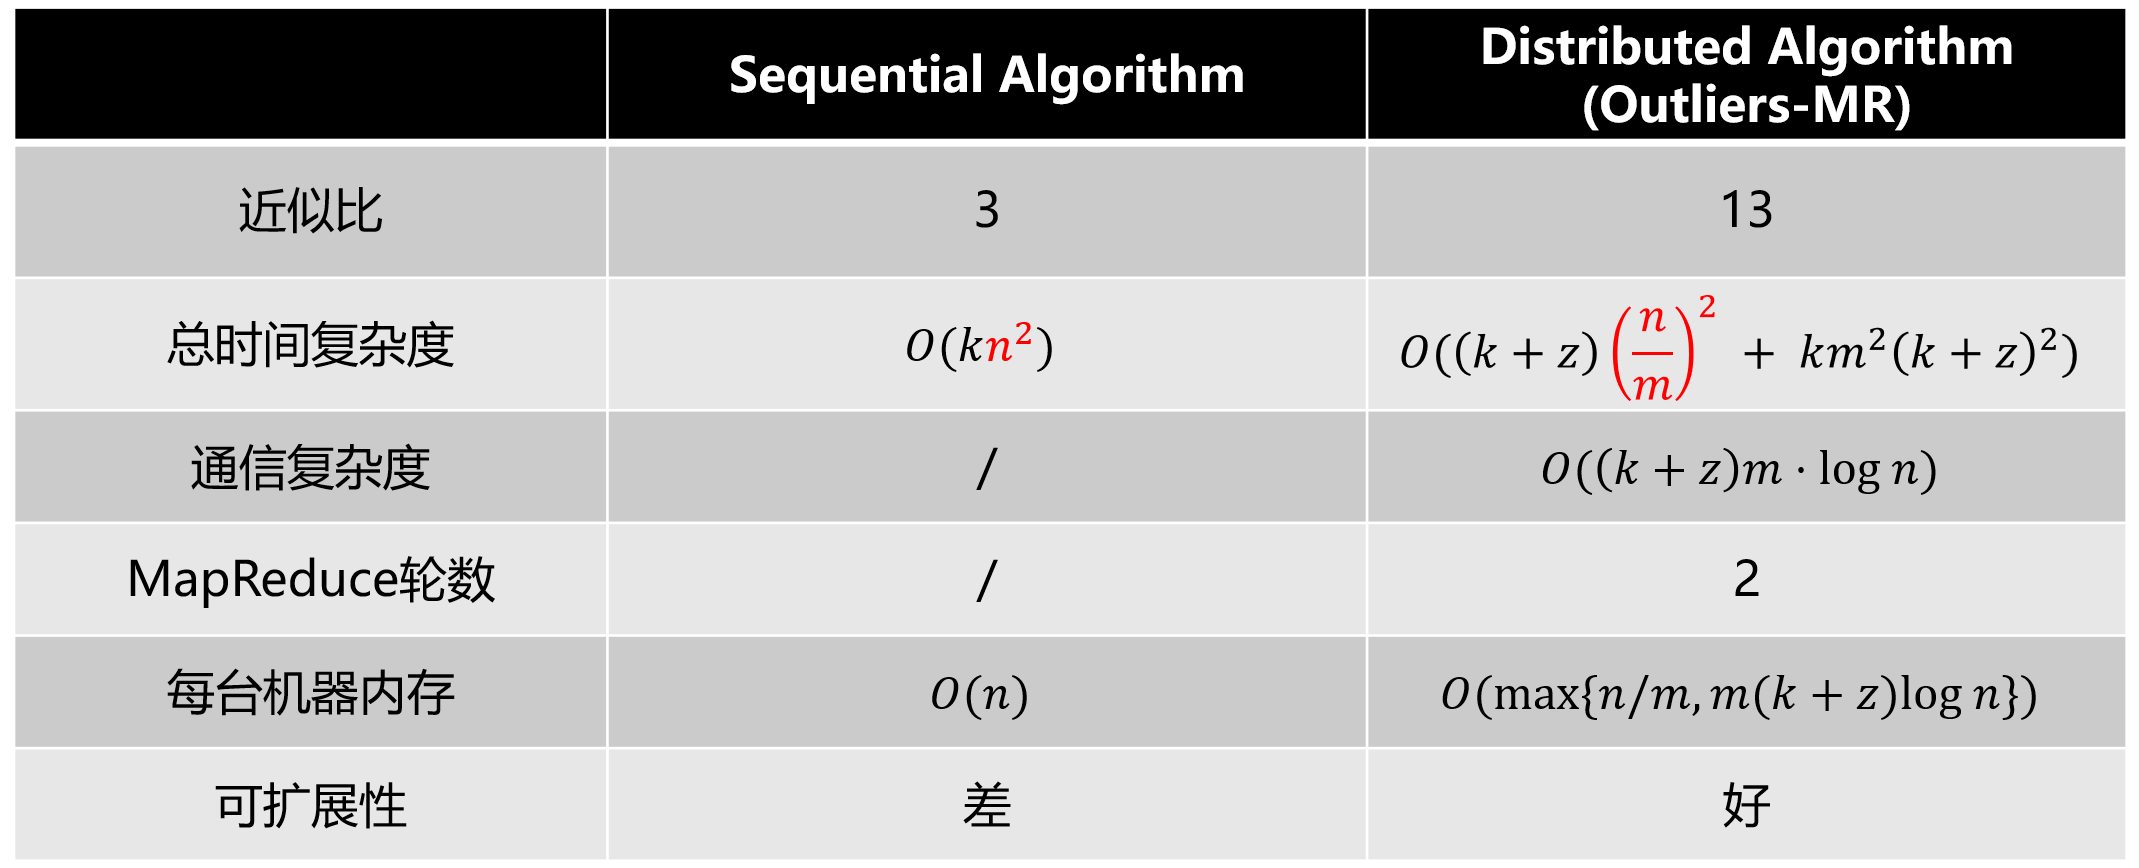
\includegraphics[width=0.8\linewidth]{figure/kcenter.png}
    \caption{分布式的Outliers-MR~\cite{malkomes2015} 算法与传统的$k$-center with outliers 算法的性能对比}
    \label{fig:kcenter}
\end{figure}

在讨论分布式 $k$-center 算法的具体实现之后，有必要介绍其背后的理论基础，尤其是关于分布式聚类问题的通信复杂度下界研究。Braverman、Feldman 和 Woodruff 等人的工作系统地揭示了：在分布式环境下，即便只求解诸如 $k$-center、$k$-median 或 $k$-means 等最基本的聚类任务，要想获得一个常数因子的近似解，机器之间必须交换相当规模的信息，其通信量下界通常在 $\Omega(k)$ 甚至 $\Omega(n)$ 级别。这意味着任何希望通过少量通信完成高质量聚类的算法，都将不可避免地面临理论上的瓶颈。

例如，Braverman、Feldman 与 Woodruff~\cite{braverman2017communication} 给出了若干统计估计与聚类问题的紧通信下界，证明在标准的 message-passing 模型中，没有分布式算法能够在显著减少通信的同时保持良好的近似比。同时，Woodruff 关于 sketching 与流式算法的综述~\cite{woodruff2014sketching} 总结了子空间嵌入、随机投影、coreset 等工具如何成为现代分布式聚类系统的理论基石。这些结果共同说明：前面介绍的“两轮 MapReduce + Gonzalez 贪心”的分布式 $k$-center 算法虽然结构简单，却已经在通信轮数与通信量方面接近理论极限，因此在实际系统中具有良好的实用性与合理性。

\subsubsection{分布式 PCA 降维}

主成分分析（Principal Component Analysis, PCA）\cite{hotelling1933analysis} 是一种经典的降维方法，用于从高维数据中提取最重要的低维特征，在图像处理、文本分析、金融数据建模等领域都有广泛应用。PCA 的核心步骤是计算数据的协方差矩阵并求其前 $k$ 个特征向量。然而在大数据场景下，PCA 计算面临严重挑战：数据分布在不同机器上，难以集中计算；协方差矩阵可能规模巨大，直接计算不可行；同时还需要在保证精度的前提下减少通信与存储成本。

\begin{figure}[htbp]
    \centering
    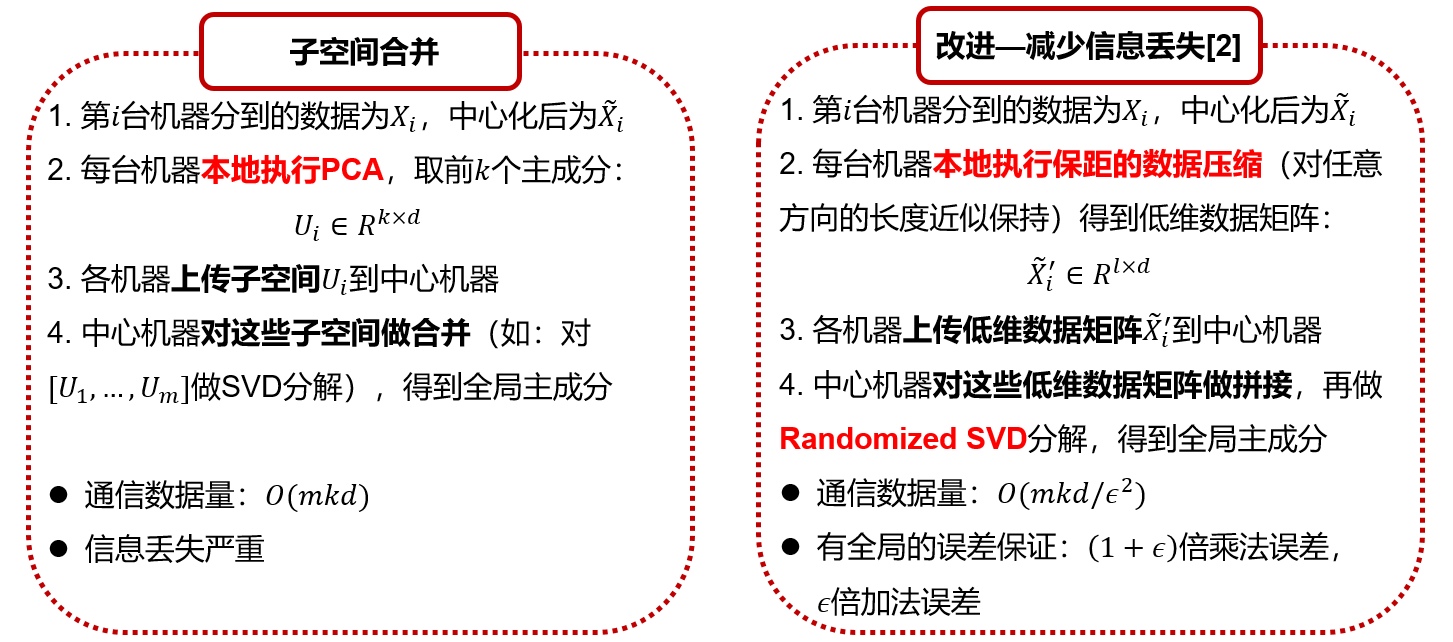
\includegraphics[width=\linewidth]{figure/distributed PCA.png}
    \caption{分布式PCA与其改进算法的基本流程}
    \label{fig:PCA}
\end{figure}

分布式 PCA 的基本思路是将传统 PCA 拆分为两个阶段：首先，各节点在本地计算其数据块的协方差矩阵，然后将这些局部结果发送到中心节点进行累加，得到全局协方差矩阵；接着，在中心节点上对全局协方差矩阵进行特征分解，得到主成分向量，并将这些向量返回给各个节点。这种方法能够充分利用分布式环境中的计算资源，并降低通信压力。改进版本的分布式 PCA（如 Liang 等人提出的方法\cite{liang2014}）还通过减少信息丢失来提升精度，各节点不仅上传协方差矩阵，还上传少量局部主成分信息，中心节点将这些信息合并后得到更接近单机 PCA 的结果，从而在通信量与精度之间取得良好平衡。

\subsubsection{分布式 PageRank}

PageRank 是 Google 早期提出的重要网页排名算法\cite{page1999pagerank}，其核心思想是“一个网页的重要性由指向它的其他网页的重要性共同决定”。它被广泛应用于搜索引擎、社交网络分析、学术引用分析等场景。然而现代互联网规模庞大，包含数百亿网页和数千亿链接，单机无法完成如此规模的计算。在单机环境中，PageRank 通常通过迭代矩阵运算实现，这在分布式场景下需要进行任务切分和并行化。

PageRank 的核心运算是稀疏矩阵与向量的乘法，非常适合并行化处理。分布式计算框架（如 MapReduce）将整个计算过程拆解为以下步骤：
\begin{enumerate}
    \item 将网页集合划分为多个子集，存储在不同节点上；
    \item 每个 Mapper 负责计算本地网页的 PageRank 值，并将结果发送给其超链接指向的目标网页；
    \item Shuffle 阶段确保同一网页的所有贡献值汇总到同一个 Reducer；
    \item Reducer 汇总贡献并更新网页的 PageRank 值；
    \item 重复以上步骤，直到整个系统收敛。
\end{enumerate}

在实现过程中，如果网页图能够被划分为边尽量不跨机器的子图，可以显著减少跨节点通信量，这是分布式 PageRank 系统设计的重要优化目标。由于 PageRank 需要多轮迭代，分布式框架通常在每轮迭代后保存中间结果以支持容错。此外，还可以通过异步迭代或增量计算进一步加速收敛。分布式 PageRank 是 MapReduce 思想的典型应用案例，展示了如何将大规模图计算分解为多个本地计算与全局汇聚过程，从而在成千上万台机器上协同完成超大规模网页排名任务。



% -------------------- 第三章 分布式机器学习训练 --------------------
\subsection{分布式机器学习训练}

随着深度学习模型和训练数据规模的持续增长，单机计算已无法满足现代机器学习任务的计算需求。以 GPT-3 为例，其模型包含约 1750 亿个参数，训练数据达到 45TB 级别，并需要数千个 GPU 同时工作，训练耗时以周计。这类任务显然无法在单台机器上完成，因此需要\textbf{分布式训练}（Distributed Training）来充分利用大规模计算集群的资源。

分布式训练的核心目标是在多个计算节点上协同完成模型训练，并通过高效的通信和同步机制，使训练效果接近甚至优于单机训练。常见的分布式训练主要分为以下两种基本模式：
\begin{enumerate}
    \item \textbf{数据并行（Data Parallelism）}：每个计算节点存放完整的模型副本，但各节点只处理不同的数据子集。每轮迭代中，各节点独立计算本地梯度，然后通过通信操作聚合这些梯度，最终同步更新模型参数。该方式适合模型较小但数据量庞大的场景。
    \item \textbf{模型并行（Model Parallelism）}：当模型本身过大，无法在单个节点的显存中完全存放时，将模型的不同部分切分到多个计算节点上，各节点负责其分配的模型片段的前向与反向传播计算。此方法常用于超大规模语言模型或多模态模型的训练。
\end{enumerate}

在实际系统中，数据并行和模型并行往往结合使用，并形成了多种分布式训练架构，其中最常见的有以下两类：

\begin{figure}[htbp]
    \centering
    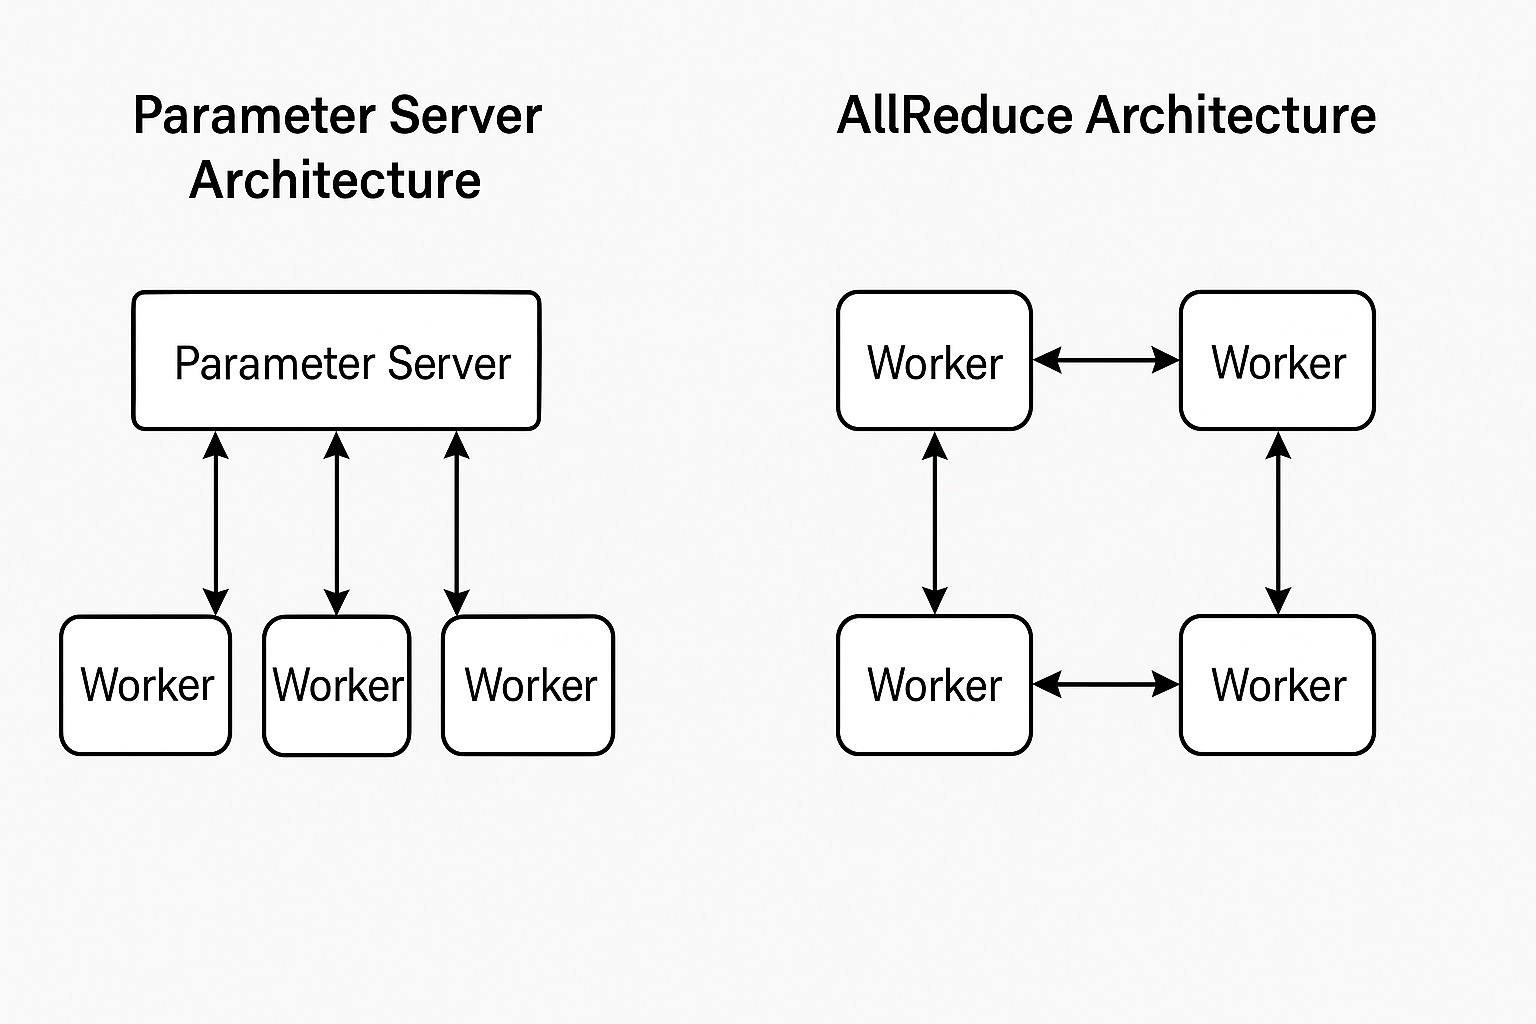
\includegraphics[width=0.7\linewidth]{figure/server.png}
    \caption{PS架构与AllReduce架构的区别}
    \label{fig:server}
\end{figure}

\textbf{（1）参数服务器（Parameter Server, PS）架构}：将模型参数集中存放在一组专门的参数服务器节点上，负责参数的存储与更新；工作节点（Worker）负责计算梯度并将结果发送给参数服务器，再由参数服务器聚合梯度并更新模型参数。PS 架构实现简单，便于扩展，但当服务器压力过大时可能成为性能瓶颈。

\textbf{（2）AllReduce 架构}：每个计算节点都保存完整的模型副本，节点之间通过 AllReduce 算法（如 Ring-AllReduce）直接通信交换梯度，实现分布式同步更新，无需中心化服务器。该架构通信效率较高，被许多深度学习框架（如 PyTorch DDP、Horovod）广泛采用。



\subsubsection{分布式训练模式：同步与异步}

在分布式机器学习训练中，多个计算节点（Worker）需要协同工作来训练统一的模型。根据各节点在训练过程中是否严格同步，可以将分布式训练分为\textbf{同步训练（Synchronous Training）}和\textbf{异步训练（Asynchronous Training）}两种模式。同步训练的核心思想是所有 Worker 节点必须在同一轮次上保持同步，每一轮更新前都要等待所有节点完成计算并交换结果，保证训练过程完全等价于单机训练的并行扩展，从而在收敛性和最终模型精度上表现稳定。其典型步骤如下：
\begin{enumerate}
    \item \textbf{模型参数广播（Broadcast）：}训练开始时，\textbf{参数服务器（Parameter Server, PS）}或主节点向所有 Worker 广播当前的全局模型参数，使每个 Worker 从同样的初始状态开始训练；
    \item \textbf{本地计算梯度（Compute Gradients）：}每个 Worker 使用本地分配的数据子集进行前向传播和反向传播，计算出本地梯度；
    \item \textbf{梯度上传与聚合（Aggregate）：}所有 Worker 完成计算后，将本地梯度发送给参数服务器或通过 AllReduce 操作进行全局求和，只有当\textbf{所有 Worker 的梯度都被收集}后才能进入下一步；
    \item \textbf{统一更新模型参数（Update）：}参数服务器根据聚合后的全局梯度更新模型参数，并将更新后的模型再次广播给所有 Worker，准备进入下一轮迭代。
\end{enumerate}

同步训练的优势是模型结果与单机训练完全一致，收敛性稳定，缺点是容易受到慢节点（Straggler）的影响，只要某一个 Worker 延迟，整个系统都必须等待，整体速度受限。

异步训练则不要求各 Worker 保持严格同步，\textbf{谁计算完成就立即上传梯度并获取最新参数}，无需等待其他节点。这种方式提高了资源利用率，但也带来了梯度陈旧（Stale Gradients）问题，可能导致模型收敛不稳定。其典型步骤如下：
\begin{enumerate}
    \item \textbf{Worker 获取模型参数（Fetch）：}Worker 在训练前向参数服务器请求最新的模型参数，不同 Worker 进度不同，因此此时获取的模型参数可能不是全局最新；
    \item \textbf{本地计算梯度（Compute）：}Worker 使用当前拿到的模型副本在本地数据上进行前向与反向传播，计算出一批数据的梯度；
    \item \textbf{上传梯度（Push）：}计算完成后，Worker 立即将梯度上传给参数服务器，无需等待其他节点；
    \item \textbf{服务器即时更新（Immediate Update）：}参数服务器接收到梯度后立即更新全局模型，并将最新版本返回给请求节点或存储为最新状态；
    \item \textbf{Worker 继续下一轮：}Worker 直接拉取更新后的模型参数，开始下一轮计算，各 Worker 速度完全独立。
\end{enumerate}

异步训练的优点是计算资源利用率高，能够显著提升吞吐量，特别适合计算资源不均衡或规模极大的集群。但由于使用的梯度可能是旧版本，容易造成模型波动甚至不收敛，为缓解这一问题，可以采用 \textbf{Stale Synchronous Parallel (SSP)} 策略，限制允许的最大延迟步数。总体而言，同步训练结果稳定，适合对精度和一致性要求高的任务；异步训练速度快，适合对实时性或大规模并行计算有较高要求的场景。通过合理选择训练模式，可以在\textbf{计算速度}与\textbf{模型精度}之间取得平衡，实现高效的分布式机器学习训练。



在实际分布式训练中，还需要考虑以下问题：
\begin{itemize}
    \item \textbf{梯度陈旧（Staleness）：}异步训练中可能出现上传梯度与最新模型不匹配的问题，过于陈旧的梯度会影响模型收敛。
    \item \textbf{慢节点问题（Stragglers）：}在同步训练中，某些节点因负载过重或网络问题导致延迟，从而拖慢整个训练过程。
    \item \textbf{带宽瓶颈：}在大规模分布式训练中，通信常常成为主要瓶颈，因此需要采用梯度压缩、混合精度训练等技术减少通信量。
\end{itemize}

\textbf{总结}：分布式机器学习训练通过并行化计算、分布式存储和高效通信，实现了超大规模模型的训练。从早期的 PS 架构到如今广泛采用的 AllReduce 框架，分布式训练技术不断发展，并成为深度学习系统设计中不可或缺的重要组成部分。实际应用中需要根据模型规模、硬件资源和任务特点选择合适的架构和同步策略，以在性能与训练质量之间取得最佳平衡。


% -------------------- 第四章 联邦学习与区块链 --------------------
\subsection{联邦学习与区块链}

\subsubsection{联邦学习}

随着数据隐私法规的日益严格和数据分布形式的不断变化，传统的集中式机器学习训练方式面临越来越多的挑战。以欧盟在 2018 年正式生效的《通用数据保护条例》（General Data Protection Regulation, GDPR）\cite{gdpr2016} 为例，该法规提出了两个核心理念：\textbf{数据不应离开数据产生地}（数据本地化原则）以及\textbf{个人数据在处理前必须获得授权，并有权被删除}。这意味着将分散在各个机构和设备上的敏感数据集中到云端服务器进行统一训练将面临法律和安全的双重障碍。类似地，美国的 HIPAA 医疗隐私法案\cite{hipaa1996}也对医疗数据的集中化存储和处理提出了严格限制。


\begin{figure}[htbp]
    \centering
    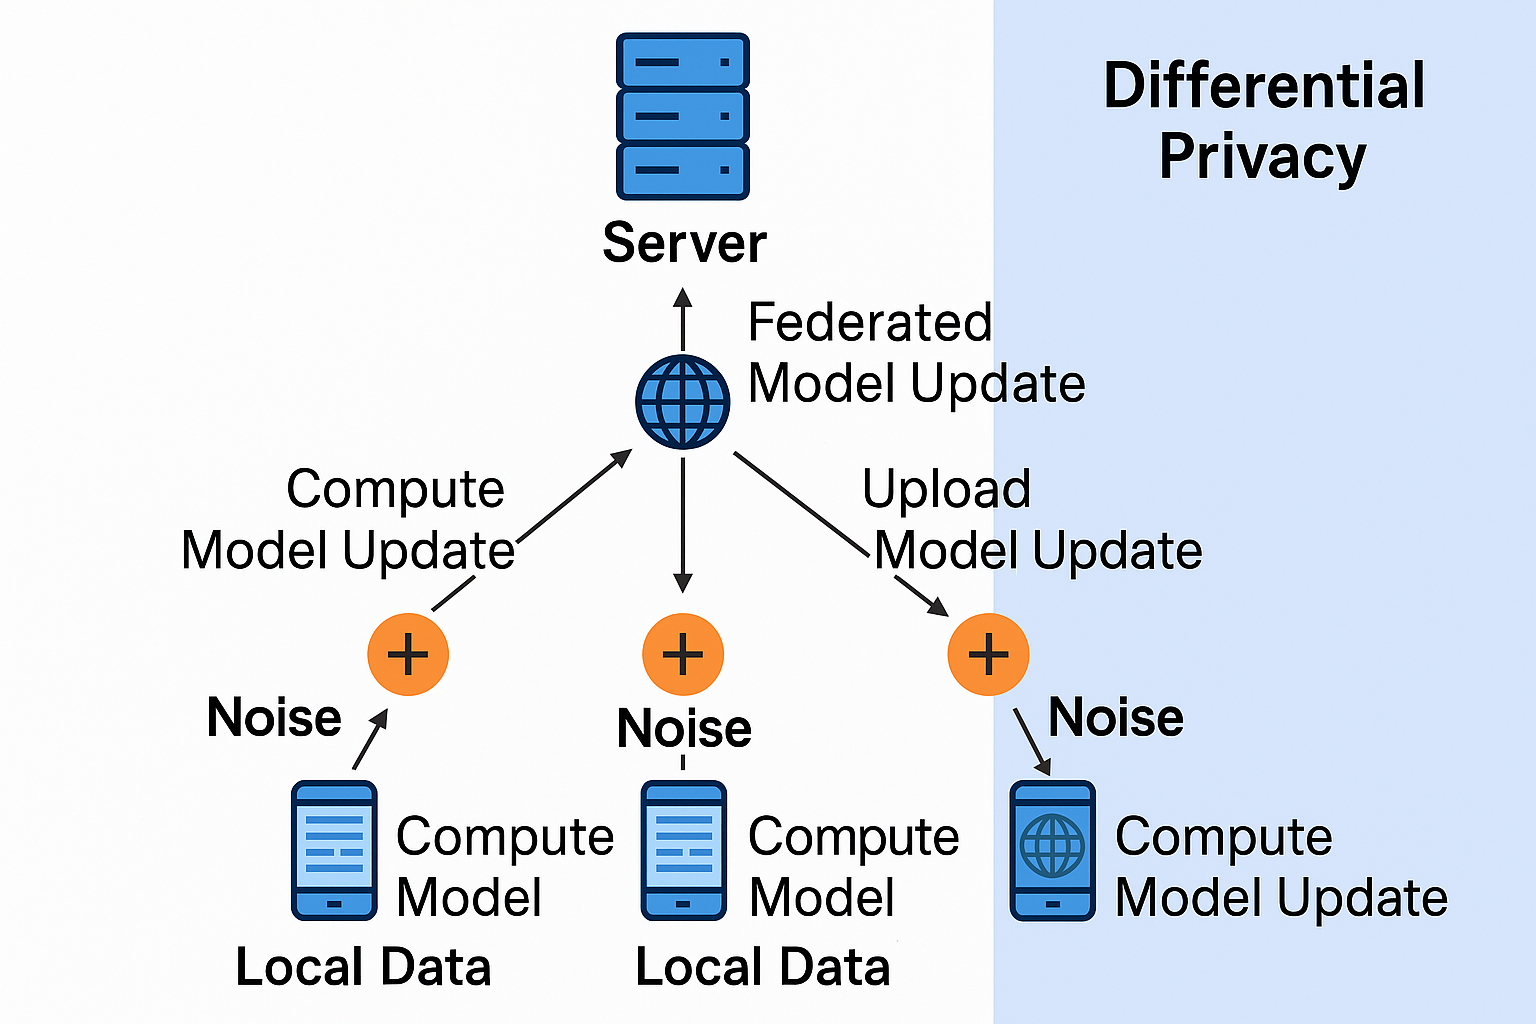
\includegraphics[width=0.7\linewidth]{figure/federated.png}
    \caption{联邦学习中的差分隐私机制示意图。每个客户端（如智能设备、医院等）在本地使用自身数据训练模型，并在上传模型更新之前通过添加噪声来实现差分隐私保护，从而防止服务器或其他客户端推断出原始数据。服务器仅接收到加入噪声后的模型更新，并对其进行聚合生成全局模型，实现“数据不出本地、隐私得以保护”的分布式协作训练过程。}

    \label{fig:federated}
\end{figure}

在实际应用中，数据越来越分散地存储在个人设备或各类组织机构中，例如：智能手机、医院、银行等。与此同时，分布式训练虽然可以在计算资源上实现协同，但并不能天然地解决\textbf{数据隐私泄露、带宽消耗以及安全}等问题。为了解决这些挑战，\textbf{联邦学习（Federated Learning, FL）} 被提出~\cite{mcmahan2017communication}，它是一种\textbf{数据不出本地、模型参数集中聚合}的机器学习训练模式，允许多个机构或设备在不共享原始数据的前提下协同训练全局模型。简单来说，联邦学习允许各参与方在不共享原始数据的前提下协同训练一个全局模型，从而在保护隐私的同时实现跨组织的数据价值整合。

联邦学习与传统的分布式训练在系统架构上存在显著差异。传统分布式训练的基本流程是：数据被划分到不同 Worker 节点，每轮迭代时每个 Worker 拉取最新模型，计算本地梯度后上传到中心节点（参数服务器），再由中心节点统一更新模型并下发最新参数。而在联邦学习中，客户端仅上传经过本地计算的模型更新信息，原始数据始终留在本地，这种方式更加符合隐私保护要求。

在实际部署中，联邦学习依赖多种隐私保护技术来进一步增强安全性：
\begin{enumerate}
    \item \textbf{差分隐私（Differential Privacy, DP）：}在客户端上传梯度或模型更新之前，先对其进行剪裁并加入噪声，使得攻击者无法根据上传信息反推出原始训练数据。差分隐私提供了严格的数学隐私保护保证，可用参数 $\varepsilon$ 定量描述隐私泄露的概率。
    \item \textbf{安全多方计算（Secure Multi-Party Computation, MPC）：}通过将梯度信息进行秘密分享，各客户端的原始梯度对任何单一方都不可见，服务器只能看到聚合后的整体结果，从而避免对单个节点的攻击。
    \item \textbf{同态加密（Homomorphic Encryption）：}客户端使用加密算法对上传的梯度进行加密，服务器无需解密即可直接在密文上完成加法聚合，这进一步保证了数据在传输和存储中的安全性。
\end{enumerate}

例如，经典的 FedSGD 框架在基本联邦学习过程中并不自动提供隐私保护，其真正的安全性依赖于上述差分隐私、MPC、同态加密等扩展机制。通过结合这些技术，可以构建一个既高效又安全的联邦学习系统。


一个典型的实际应用是 \textbf{Split Neural Network (SplitNN)}~\cite{gupta2018}，其通过分割模型结构，使得客户端仅上传中间特征表示而非原始数据，从而进一步减少隐私泄露风险。在 SplitNN 中，神经网络被分为多个部分，前半部分运行在客户端设备上，后半部分运行在服务器上。训练过程中，客户端只需上传\textbf{中间特征表示}而不是原始数据，服务器也仅返回单层梯度给客户端。这种方式进一步缩小了潜在隐私泄露的范围。相比传统分布式神经网络中完整梯度的上传，SplitNN 只暴露更抽象、更高层次的中间信息，从而更好地保护隐私。此外，SplitNN 还可以针对不同计算设备的能力进行自适应划分，提升系统灵活性。

\subsubsection{区块链}

除了隐私保护，\textbf{去中心化的数据管理}也是联邦学习发展的重要方向。近年来，研究者们也将\textbf{区块链技术}引入联邦学习，以应对多参与方协作中的信任问题~\cite{xu2019federated}，并利用区块链的不可篡改特性记录模型更新历史。区块链技术提供了一种无需中心化机构的分布式账本机制，可以天然适配联邦学习的多参与方协作场景。区块链的核心特点包括：每个区块包含交易数据、上一个区块的哈希值和时间戳，通过共识机制（如工作量证明 Proof of Work, PoW）实现全网一致性，一旦数据上链便不可篡改。将区块链引入联邦学习，可以实现以下功能：
\begin{enumerate}
    \item 记录各客户端的模型更新行为，确保溯源和责任追踪；
    \item 通过智能合约实现模型更新规则的自动执行；
    \item 利用去中心化共识减少对中心服务器的信任需求。
\end{enumerate}

例如，在一个基于区块链的联邦学习系统中，模型更新记录被打包进区块并广播到所有参与节点，任何节点都可以验证模型更新的合法性，从而防止恶意节点上传虚假模型。这不仅提高了系统的透明度和可信度，也使联邦学习在金融、医疗等高安全要求领域更具可行性。

总而言之，联邦学习结合了分布式训练和隐私保护的优势，是应对现代数据分散化和隐私法规要求的重要解决方案。而区块链为联邦学习提供了去中心化的信任基础和安全记录机制，二者的结合有望推动未来跨组织、跨行业的智能协作与数据价值共享。


% -------------------- 结论 --------------------
\subsection{总结与展望}
分布式算法是现代大数据处理的核心。从k-center聚类、PCA到分布式深度学习与联邦学习，分布式算法不断发展，并在未来与隐私计算、区块链等技术融合，推动人工智能在更加严格的数据保护环境下发展。



\section{重心估计}
在训练大模型的时候，SGD（随机梯度下降）是一种简单有效的优化算法。SGD的关键是计算得到模型参数关于训练数据的梯度信息，然后根据梯度信息更新模型参数。在分布式的场景下，每一个分布式节点都有一个模型的副本，各个节点根据自己的数据计算模型的梯度信息，然后将各自的梯度信息传输给中心服务器。中心服务器根据这些梯度信息求一个均值（或者加权均值），然后根据均值（或者加权均值）更新模型参数，并将模型参数分发给子节点。在这个场景里，节点和中心服务器的通信开销是巨大的，这是制约模型训练的瓶颈。因此，各个子节点如何尽可能的压缩梯度信息，并且使得中心服务器根据这些压缩后的梯度尽可能准确的计算梯度均值是一个重要的问题，这个问题就是本节要讨论的问题，Mean Estimation，即重心估计。


\subsection{问题定义}

\paragraph{模型描述} 假设在d维欧式空间$R^d$中存在 $n$ 个向量$\{x_{1},x_{2},...,x_{n}\}$，每一个向量是一个分布式节点上的梯度信息向量。每一个节点i通过函数$f$来压缩自己的梯度向量为$f(x_{i})$，中心服务器根据函数$g$来解压缩每一个节点传来的梯度向量信息$g(f(x_{i}))$。

\paragraph{目标} 使得通信开销$\sum_{i=1}^n f(x_{i})$尽可能小，同时尽可能减小重心的期望估计误差
\[min E(||\hat{\bar{X}} - \bar{X}||_{2}^2)\]
其中$\bar{X} = \frac{1}{n} \sum_{i=1}^n x_{i}$表示精确的重心，$\hat{\bar{X}} =  \frac{1}{n} \sum_{i=1}^n g(f(x_{i}))$表示估计的重心

如果一个实数使用$L$ bits来表示，那么对向量信息不进行任何处理，直接传输的通信开销为$\mathcal{O}(ndL)$

\begin{remark}
对于这个问题，一个直接的想法是JL变换，它可以压缩节点的向量信息，降低通信开销。但是，由于JL变换只具有压缩功能，我们无法根据JL变换的压缩结果解压出原始的向量信息，因此就无法估计向量的重心，故在这个问题里JL变换是不可行的。 
\end{remark}

\subsection{Stochastic Binary Quantization算法}

\paragraph{基本思路} Stochastic Binary Quantization算法，即随机二值量化算法，其基本思路是将每一个实数值随机量化为两个数值$t_{1},t_{2}$中的一个，因此对于一个$d$维向量，我们只需要存储$d$个01变量，表示他们是$t_{1},t_{2}$中的哪一个即可。这样，我们便可以降低存储向量的代价，进而降低通信开销。

\paragraph{算法过程} 对于任何一个$x_{i}$,令
\[x_{i}^{max} = max_{1 \leq j \leq d} x_{i}(j)\]
\[x_{i}^{min} = min_{1 \leq j \leq d} x_{i}(j)\]
其中$x_{i}(j)$表示向量$x_{i}$的第$j$位。根据这个计算$y_{i}$如下：
\begin{align}
\nonumber
y_{i}(j) = \left\{
\begin{aligned}
\nonumber
&x_{i}^{max}  &\text{以概率}\frac{x_{i}(j) - x_{i}^{min}}{x_{i}^{max} - x_{i}^{min}}\\
&x_{i}^{min}  &\text{以概率}\frac{x_{i}^{max} - x_{i}(j)}{x_{i}^{max} - x_{i}^{min}}\\
\end{aligned}
\right.
\end{align}

于是我们将$x_{i}$通过上面的方法压缩成了$y_{i}$,即$y_{i} = f(x_{i})$

\paragraph{算法分析} 接下来我们分析算法得到的估计的重心的准确性
\[
E(y_{i}(j)) = x_{i}^{max}\frac{x_{i}(j) - x_{i}^{min}}{x_{i}^{max} - x_{i}^{min}} + x_{i}^{min}\frac{x_{i}^{max} - x_{i}(j)}{x_{i}^{max} - x_{i}^{min}} = x_{i}(j)
\]
于是得到：
\[
E(\hat{\bar{X}}) = \frac{1}{n} \sum_{i = 1}^{n} y_{i} = \bar{X}
\]
\begin{align*}
    E(||\hat{\bar{X}} - \bar{X}||_{2}^2)
    &= \frac{1}{n^2} E(||\sum_{i =1}^{n}(y_{i} - x_{i})||_{2}^2)\\
    &= \frac{1}{n^2} \sum_{i=1}^{n}E(||y_{i} - x_{i}||_{2}^2)\\
    &= \frac{1}{n^2} \sum_{i=1}^{n} \sum_{j = 1}^{d} E((y_{i}(j) - x_{i}(j))^2)\\
    &= \frac{1}{n^2} \sum_{i=1}^{n} \sum_{j = 1}^{d} (x_{i}^{max} - x_{i}(j))(x_{i}(j) - x_{i}^{min})\\
    &\leq \frac{1}{n^2} \sum_{i=1}^{n} \sum_{j = 1}^{d} \frac{(x_{i}^{max} - x_{i}^{min})^2}{4}\\
    &\leq \frac{d}{2n^2} \sum_{i =1}^{n}||x_{i}||_{2}^2\\
\end{align*}

梯度向量的维度d表示模型的参数数 量，一般来说，模型的参数数量是巨大的，因此，d一般比较大，远远大于n，所以这个算法得到的bound是一个非常粗的的bound

该算法对于每一个向量$x_{i}$,需要存储两个实数$x_{i}^{max}$和$x_{i}^{min}$,这需要$2L$bits,还需要存储一个$d$维01向量表示每一维，因此需要$d + 2L$bits的存储空间，一共有$n$个向量，因此总共需要$\mathcal{O}(n(d + 2L))$的存储空间。因此通信开销也就是$\mathcal{O}(n(d + 2L))$
\subsection{Stochastic K-level Quantization算法}
Stochastic Binary Quantization算法将每个向量的每一维都映射成两个值，$x_{i}^{max}$和$x_{i}^{min}$，这导致算法估计的重心与精确重心误差较大，一个直接的改进方法是，将Binary改进为K-level，即将每个向量的每一维都映射成更细化的多个等级的值，这就是Stochastic K-level Quantization算法的主要思想

\paragraph{算法过程} 对于任何一个$x_{i}$,令
\[x_{i}^{max} = max_{1 \leq j \leq d} x_{i}(j)\]
\[x_{i}^{min} = min_{1 \leq j \leq d} x_{i}(j)\]
假设我们将该向量的每一维都映射成$k$个等级的值中的一个，那么相当于将区间$[x_{i}^{min},x_{i}^{max}]$均匀的划分成$k - 1$个子区间，假设$x_{i}(j)$落在第$t$个子区间内，其中$t \in \{0,1,2,...t-1\}$，那么根据这个计算$y_{i}$如下：
\begin{align}
\nonumber
y_{i}(j) = \left\{
\begin{aligned}
\nonumber
&x_{i}^{min} + t\frac{S_{i}}{k}  &\text{以概率}\frac{x_{i}^{min} + (t + 1)\frac{S_{i}}{k} - x_{i}(j)}{\frac{S_{i}}{k}}\\
&x_{i}^{min} + (t + 1)\frac{S_{i}}{k}  &\text{以概率}\frac{x_{i}(j) - (x_{i}^{min} + t\frac{S_{i}}{k})}{\frac{S_{i}}{k}}\\
\end{aligned}
\right.
\end{align}
其中$S_{i} = x_{i}^{max} - x_{i}^{min}$是区间长度,于是我们将$x_{i}$通过上面的方法压缩成了$y_{i}$,即$y_{i} = f(x_{i})$

经过K-level改进后，该算法估计的重心错误率bound为$\frac{d}{2n^2k^2} \sum_{i =1}^{n}||x_{i}||_{2}^2$，即：
\[
E(||\hat{\bar{X}} - \bar{X}||_{2}^2) \leq \frac{d}{2n^2k^2} \sum_{i =1}^{n}||x_{i}||_{2}^2
\]
改进后，每一个向量的每一维需要记录它属于k个等级的值的哪一个，因此需要$\log k$的存储空间，故算法总共的通信复杂度为$\mathcal{O}(n(d\log k + 2L))$

\subsection{Stochastic Rotated Quantization算法}
该算法基于一个几何上的结论：假设$||x_{i}||^2_{2} = 1$，$x_{i}$在$d$维单位球上随机地旋转，那么以很高的概率有$x_{i}^{max} - x_{i}^{min} = \mathcal{O}(\sqrt{\frac{\log d}{d}})$


回忆之前讲过的FJLT的内容，我们当时为了加速JL变换，希望变换矩阵P是稀疏的，然而，当P是稀疏的，待变换的输入向量也是稀疏的时候，变换的结果会产生较大的误差，因此，我们希望输入的向量是稠密的。但是，输入向量的稀疏与否不可控制，因此我们可以在输入向量进行JL变换之前乘以一个随机旋转矩阵，依赖于这个几何结论，可以使得输入向量变得稠密，从何实现加速JL变换过程，又不显著增加误差的目的。在FJLT中，我们使用的随机旋转矩阵是 $\mathbf{H}\cdot \mathbf{D}$，其中$\mathbf{H}$是Hadamard矩阵，$\mathbf{D}$是一个随机对角方阵。（详细构造方法可以参考FJLT章节的内容）


类似的，我们也可以将向量$x_{i}$进行随机旋转，这样可以使得向量变得稠密，从而减小$x_{i}^{max} - x_{i}^{min}$，根据之前的计算重心估计的误差的过程，我们于是可以减少重心估计的误差
\paragraph{算法过程} 我们首先获得一个随机旋转矩阵$R$，对于任何一个$x_{i}$,将随机旋转矩阵$R$作用到$x_{i}$上，得到$Rx_{i}$,然后，对$Rx_{i}$向量采用Stochastic K-level Quantization算法得到$y_{i}$，并将量化的结果$y_{i}$传输给中心服务器。中心服务器首先将$y_{i}$逆旋转得到$R^{-1}y_{i}$，然后计算重心为
\[
\hat{\bar{X}} = \frac{1}{n}\sum_{i = 1}^{n} R^{-1}y_{i}
\]
由于该算法在传输数据时，传输的是K-level算法的结果，因此通信复杂度和Stochastic K-level Quantization算法一样，都是$\mathcal{O}(n(d\log k + 2L))$，但是由于随机旋转有
\[
x_{i}^{max} - x_{i}^{min} = \mathcal{O}(\sqrt{\frac{\log d}{d}})
\]
而我们之前在计算Stochastic Binary Quantization算法估计的重心误差bound时，有
\[
 E(||\hat{\bar{X}} - \bar{X}||_{2}^2) = \leq \frac{1}{n^2} \sum_{i=1}^{n} \sum_{j = 1}^{d} \frac{(x_{i}^{max} - x_{i}^{min})^2}{4}
\]
因此，该算法估计的重心误差bound为$\mathcal{O}(\frac{\log d}{n^2k^2} \sum_{i =1}^{n}||x_{i}||_{2}^2)$，即：
\[
E(||\hat{\bar{X}} - \bar{X}||_{2}^2) \leq \mathcal{O}(\frac{\log d}{n^2k^2} \sum_{i =1}^{n}||x_{i}||_{2}^2)
\]

参考文章\cite{suresh2017distributed}。








\printbibliography[heading=subbibliography, title={本章参考文献}]
\addcontentsline{toc}{section}{参考文献} % 手动添加到目录
\end{refsection}

\begin{refsection}
\chapter{Beyond worst case analysis}

\section{k-means问题}
\subsection{问题背景}

传统算法分析大多关注\textbf{最坏情况复杂度（worst-case complexity）}。最坏情况分析能够为算法提供理论上的性能保障，但在许多实际问题中，这种分析往往过于保守，不能很好地反映算法在真实数据上的表现。例如，$k$-means 算法在最坏情况下是 NP-hard，且经典 Lloyd 算法在理论上可能陷入局部最优且收敛缓慢 \cite{arthur2006kmeans, vattani2011hardness}，然而在实际应用中它却表现得非常高效且稳定。这一现象表明：\textbf{最坏情况分析与实际表现之间存在巨大差距}。为了弥合这一差距，近年来理论计算机科学领域提出了\textbf{超越最坏情况分析（Beyond Worst-Case Analysis, BWCA）}的研究框架 \cite{roughgarden2021beyond}，其目标是在最坏情况分析和平均情况分析之间找到一种平衡，更加精细地刻画现实问题的结构特征，并在此基础上给出更符合实际的数据驱动理论保证。

现实世界中的数据往往并非完全对抗性的，因此直接使用最坏情况假设显得过于悲观。例如在聚类问题中，许多实际数据集往往存在天然的\textbf{簇结构}（cluster structure），而这种结构可以被算法所利用，从而显著提升聚类的理论可解释性和效率。BWCA 的研究动机主要体现在以下三个方面：1）\textbf{实践驱动}：如 Lloyd 算法在图像识别、医疗数据分析等领域应用广泛，其良好的实验表现需要得到理论解释；2）\textbf{理论挑战}：许多经典问题如 $k$-means、$k$-median、社区检测等在最坏情况下都具有很高的计算复杂度，研究如何通过额外假设降低复杂度成为重要问题；3）\textbf{泛化能力}：相比单纯的最坏情况分析，BWCA 通过引入结构化假设，更容易与机器学习理论结合，为数据驱动的算法设计提供新的思路 \cite{awasthi2012stability, balcan2013clustering}。

在 BWCA 框架下，研究者提出了多种分析模型来刻画数据的“良好结构”，以下是几类具有代表性的假设和分析模型：
\begin{enumerate}
    \item \textbf{稳定性（Stability）假设}：Bilu 和 Linial 在图分割问题中首次提出了稳定性假设 \cite{bilu2010stability}。其核心思想是：如果一个实例的最优解在轻微扰动下保持不变，那么该实例被认为是“稳定的”。在这种情况下，算法可以利用这种稳定性结构，在多项式时间内求得全局最优解。例如，在 $k$-means 聚类中，如果数据满足 $\alpha$-稳定性条件，则可以设计出近似或精确算法 \cite{awasthi2012stability}。这一假设为解释 Lloyd 算法在实际中高效表现提供了理论基础。

    \item \textbf{分离性（Separation）假设}：另一类广泛使用的假设是分离性，即不同簇之间的距离足够大，从而保证簇结构明显。例如，Balcan 等人提出的 $\gamma$-margin 假设要求每个点到其所属簇中心的距离显著小于到其他簇中心的距离 \cite{balcan2013clustering}。在这种条件下，许多启发式算法（如 Lloyd 算法）都可以被严格证明在多项式时间内得到近似最优的聚类结果 \cite{ostrovsky2012effectiveness}。

    \item \textbf{扰动弹性（Perturbation Resilience）假设}：Perturbation Resilience 是稳定性的一种推广形式，由 Balcan 等人提出 \cite{balcan2009perturbation}，其定义为：如果将数据集中所有距离按照一定比例轻微扰动后，原问题的最优解保持不变，则称该实例具有扰动弹性。这种假设在解释实际数据的鲁棒性方面尤为重要，尤其是在聚类与社区检测问题中，具有扰动弹性的实例通常可以在多项式时间内求解，并能抵御噪声和数据偏差的影响。

    \item \textbf{平滑分析（Smoothed Analysis）}：Spielman 和 Teng \cite{spielman2004smoothed} 提出了平滑分析框架，它介于最坏情况与平均情况之间。具体而言，该模型允许对输入数据进行小幅随机扰动，并分析扰动后的期望运行时间。平滑分析成功解释了单纯形法（Simplex Method）在实际中表现良好的原因，同时也被用于解释 Lloyd 算法在 $k$-means 聚类中的良好实际表现 \cite{arthur2006kmeans}。
\end{enumerate}

$k$-means 是 BWCA 的经典研究对象之一。一方面，Lloyd 算法在最坏情况下收敛缓慢，但在稳定性、分离性或扰动弹性假设下，可以在多项式时间内找到近似最优解 \cite{awasthi2012stability, ostrovsky2012effectiveness, balcan2009perturbation}；另一方面，对 $k$-means 的 BWCA 分析帮助研究者理解了其在图像识别、医疗数据分析等领域的良好实际表现，并促进了公平聚类、动态聚类等扩展问题的研究。在接下来的内容中，我们将以 $k$-means 聚类为例，深入探讨如何将 BWCA 的理念应用于具体的算法分析和设计中。


\subsection{基本知识}

\begin{definition}
    $\text{若 } \Delta_k^2(X) \leq \varepsilon^2 \Delta_{k-1}^2(X), \text{ 则称 } X \text{ 是 } \varepsilon\text{-Separated}.$ 其中，$X$ 表示 $\mathbb{R}^d$ 中的 $n$ 个输入点构成的集合，$\Delta_k^2(X)$ 表示对 $X$ 进行 $k$-means 聚类时所得的最小代价（即最优解的 cost）\cite{ostrovsky2013effectiveness}。
\end{definition}

\begin{lemma}
    对于任意点集 $X = \{x_1, \dots, x_n\} \subset \mathbb{R}^d$，定义其均值为：
\[
\mu(X) = \frac{1}{n} \sum_{x \in X} x,
\]
则有以下恒等式成立：
\[
\forall x \in X,\quad \sum_{y \in X} \|x - y\|^2 = \Delta_1^2(X) + n \|x - \mu(X)\|^2,
\]
进而有：
\[
\sum_{x \in X} \sum_{y \in X} \|x - y\|^2 = n\Delta_1^2(X) + n \sum_{x \in X} \|x - \mu(X)\|^2.
\]
注意到右侧第二项等于 $n \Delta_1^2(X)$，因此：
\[
\sum_{x \in X} \sum_{y \in X} \|x - y\|^2 = n \Delta_1^2(X) + n \Delta_1^2(X) = 2n \Delta_1^2(X).
\]
\end{lemma}

\begin{lemma}
    设点集 $X$ 被划分为两个子集 $X_1$ 和 $X_2$，记 $n_1 = |X_1|$, $n_2 = |X_2|$, $n = |X|$，则：

\begin{enumerate}
  \item $\Delta_1^2(X) = \Delta_1^2(X_1) + \Delta_1^2(X_2) + \frac{n_1 n_2}{n} \left\| \mu(X_1) - \mu(X_2) \right\|^2$
  
  \item $ \left\| \mu(X_1) - \mu(X) \right\|^2 \leq \frac{\Delta_1^2(X)}{n} \cdot \frac{n_2}{n_1}$

\end{enumerate}
\end{lemma}

\subsection{The 2-Means Problem}

设 $k = 2$，$\mu_1, \mu_2$ 为最佳的两个子簇中心点。

\textbf{假设：}
\[
\Delta_2^2(X) \leq \varepsilon^2 \Delta_1^2(X)
\]

\textbf{算法：}

\begin{enumerate}
    \item \textbf{采样（Sampling）：} 从集合 $X$ 中随机选取一对点作为初始中心，选取点对 $x, y \in X$ 的概率与 $\|x - y\|^2$ 成正比($\frac{\|x - y\|^2}{\sum_{x, y \in X} \|x - y\|^2}$)。设 $\hat{\mu}_1, \hat{\mu}_2$ 为选出的两个中心点。
    
    \item \textbf{“Ball-k-Means” 步骤：} 对于每个 $\hat{\mu}_i$，以其为中心、半径为 $r = \|\hat{\mu}_1 - \hat{\mu}_2\| / 3$ 的球中，计算集合 $X$ 在该球内部分的质心，记为 $\bar{\mu}_i$。返回 $\bar{\mu}_1, \bar{\mu}_2$ 作为最终中心。
\end{enumerate}


\textbf{运行时间（Running Time）}： 整个算法的运行时间为 $O(nd)$。步骤 (2) 显然只需 $O(nd)$ 时间。我们将证明：采样步骤可以在 $O(nd)$ 时间内实现。

考虑以下的两步采样过程：  
\begin{itemize}
    \item[(a)] 首先，从集合 $X$ 中选择一个点 $x$，其被选中的概率为：
    \[
    \frac{\sum_{y \in X} \|x - y\|^2}{\sum_{x, y \in X} \|x - y\|^2} 
    = \frac{\Delta_1^2(X) + n \|x - \mu(X)\|^2}{2n \Delta_1^2(X)}
    \]
    （由引理 1.2 得出）；
    
    \item[(b)] 然后，从 $X$ 中选择第二个中心 $y$，其被选中的概率为：
    \[
    \frac{\|y - \hat{\mu}_1\|^2}{\Delta_1^2(X) + n \|\mu(X) - \hat{\mu}_1\|^2}
    \]
\end{itemize}

这个两步采样过程等价于步骤 (1) 中的采样过程，即以如下概率选择点对 $x_1, x_2 \in X$：
\[
\frac{\|x_1 - x_2\|^2}{\sum_{(x, y) \in X} \|x - y\|^2}
\]

由于 $\Delta_1^2(X)$ 可预先计算，因此每一步都只需 $O(nd)$ 时间。

\begin{lemma}
    $\max(r_1^2, r_2^2) \leq \frac{\varepsilon^2}{1 - \varepsilon^2} \|\mu_1 - \mu_2\|^2 = O(\varepsilon^2) \|\mu_1 - \mu_2\|^2.$ 其中 $r_i^2 = \frac{\Delta_1^2(X_i)}{n_i}
$
\end{lemma}

\begin{proof}
    根据引理 1.3 的第 (1) 点，有  
\[
\Delta_1^2(X) = \Delta_2^2(X) + \frac{n_1 n_2}{n} \|\mu_1 - \mu_2\|^2,
\]  
这等价于  
\[
\frac{n}{n_1 n_2} \cdot \Delta_2^2(X) = \frac{\|\mu_1 - \mu_2\|^2 \cdot \Delta_2^2(X)}{\Delta_1^2(X) - \Delta_2^2(X)}.
\]  
这意味着：
\[
r_1^2 \cdot \frac{n}{n_2} + r_2^2 \cdot \frac{n}{n_1} \leq \frac{\varepsilon^2}{1 - \varepsilon^2} \|\mu_1 - \mu_2\|^2.
\quad 
\]
\end{proof}

\noindent \textbf{假设} $\rho = \frac{100 \varepsilon^2}{1 - \varepsilon^2}$，我们要求 $\rho < \frac{1}{4}$，因此 $\varepsilon^2 < \frac{1}{401}$。我们定义簇 $X_i$ 的核心为：
\[
X_i^{\text{cor}} = \left\{ x \in X_i : \|x - \mu_i\|^2 \leq \frac{r_i^2}{\rho} \right\}.
\]  
由 Markov 不等式可知，$\left|X_i^{\text{cor}}\right| \geq (1 - \rho)n_i$，对 $i = 1, 2$ 成立。

\begin{lemma}
    $\Pr\left[\{\hat{c}_1, \hat{c}_2\} \cap X_1^{\text{cor}} \neq \varnothing \quad \text{且} \quad \{\hat{c}_1, \hat{c}_2\} \cap X_2^{\text{cor}} \neq \varnothing \right] \geq 1 - 4\rho.$
\end{lemma}

\begin{proof}
为简化表达，我们假设所有点按 $\frac{1}{\|\mu_1 - \mu_2\|}$ 缩放（因此 $\|\mu_1 - \mu_2\| = 1$）。

由引理 1.3 的 (1) 部分可得：
\[
\Delta_1^2(X) = \Delta_2^2(X) + \frac{n_1 n_2}{n} \|\mu_1 - \mu_2\|^2
\Rightarrow \Delta_1^2(X) \leq \frac{n_1 n_2}{n(1 - \varepsilon^2)}
\quad \text{（因为 } \Delta_2^2(X) < \varepsilon^2 \Delta_1^2(X) \text{）}.
\]

令 $\mu_i'$ 为 $X_i^{\text{cor}}$ 的质心。由引理 1.3 (2)（令 $S = X_i$，$S_1 = X_i^{\text{cor}}$）有：
\[
\|\mu_i' - \mu_i\|^2 \leq \frac{\rho}{1 - \rho} r_i^2.
\]

记事件发生的概率为 $A / B$，其中
\[
A = \sum_{x \in X_1^{\text{cor}}} \sum_{y \in X_2^{\text{cor}}} \|x - y\|^2
= \sum_{x \in X_1^{\text{cor}}} \left( \Delta_1^2(X_2^{\text{cor}}) + |X_2^{\text{cor}}| \|x - \mu_2'\|^2 \right),
\]
整理得：
\[
A = |X_1^{\text{cor}}| \Delta_1^2(X_2^{\text{cor}}) + |X_2^{\text{cor}}| \Delta_1^2(X_1^{\text{cor}}) + |X_1^{\text{cor}}| |X_2^{\text{cor}}| \|\mu_1' - \mu_2'\|^2 \geq (1 - \rho)^{2} n_1 n_2  \|\mu_1' - \mu_2'\|^2 .
\]

\[
B = \sum_{(x, y) \subseteq X} \|x - y\|^2 = n \Delta_1^2(X) \leq \frac{n_1 n_2}{1 - \varepsilon^2}.
\]

结合 Lemma 2.1 以及 $\|\mu_i' - \mu_i\|$ 的上界，可得：
\[
\|\mu_1' - \mu_2'\| \geq \|\mu_1 - \mu_2\| - 2 \cdot \frac{\rho}{1 - \rho} \max(r_1, r_2)
\geq 1 - 2 \varepsilon \sqrt{\frac{\rho}{(1 - \rho)(1 - \varepsilon^2)}} \geq 1 - \frac{\rho}{5 \sqrt{1 - \rho}}.
\]

综上：
\[
A \geq \left(1 - 2\rho - \frac{2\rho}{5 \sqrt{1 - \rho}} \right) n_1 n_2, 
\quad \text{且} \quad \frac{A}{B} \geq 1 - 4\rho. 
\]
\end{proof}

\begin{lemma}
 对于任意的$i$，我们有$X_i^{\text{cor}} \subseteq B_i \subseteq X_i\mathcncomma
\quad \text{因此} \quad \|\bar{\mu}_i - \mu_i\|^2 \leq \frac{\rho}{1 - \rho} \cdot r_i^2$。 其中$B_i = \left\{ x \in X : \|x - \hat{\mu}_i\| \leq \frac{\|\hat{\mu}_1 - \hat{\mu}_2\|}{3} \right\}$.
\end{lemma}

\begin{proof}
    令
\[
\theta = \frac{\varepsilon}{\sqrt{\rho (1 - \varepsilon^2)}} \leq \frac{1}{10}\mathcnperiod
\]
根据引理 2.1，可得：
\[
\|\hat{\mu}_i - \mu_i\| \leq \sqrt{ \frac{\rho}{1 - \rho} } \cdot r_i \leq \theta \|\mu_1 - \mu_2\|, \quad \text{对 } i = 1, 2\mathcnperiod
\]
因此：
\[
\frac{4}{5}\leq \frac{\|\hat{\mu}_1 - \hat{\mu}_2\|}{\|\mu_1 - \mu_2\|} \leq \frac{6}{5}.
\]
对任意 $x \in B_i$，有：
\[
\|x - \mu_i\| \leq \|x - \hat{\mu}_i\| + \|\hat{\mu}_i - \mu_i\| 
\leq \frac{\|\mu_1 - \mu_2\|}{2}\mathcncomma
\]
所以 $x \in X_i$。
对于任意 $x \in X_i^{\text{cor}}$，由于：
\[
\|x - \hat{\mu}_i\| \leq 2\theta \|\mu_1 - \mu_2\| \leq \frac{\|\hat{\mu}_1 - \hat{\mu}_2\|}{3}\mathcncomma
\]
所以 $x \in B_i$。 因此有 $X_i^{\text{cor}} \subseteq B_i \subseteq X_i$。

根据引理 1.3 的第(2)部分，取 $S = X_i$，$S_1 = B_i$，并注意 $|B_i| \geq |X_i^{\text{cor}}|$，可得：
\[
\|\bar{\mu}_i - \mu_i\|^2 \leq \frac{\rho}{1 - \rho} \cdot r_i^2\mathcnperiod
\]
\end{proof}

\begin{theorem}
    该算法返回的聚类，其代价最多为：
\[
\frac{\Delta_2^2(X)}{1 - \rho},
\]  
并且以至少 $1 - O(\rho)$ 的概率成功，算法运行时间为 $O(nd)$，其中：
\[
\rho = \frac{100 \varepsilon^2}{1 - \varepsilon^2}\mathcnperiod
\]
\end{theorem}

\begin{proof}
    该解的总损失至多为：
\[
\sum_{i,\,x \in X_i} \|x - \bar{\mu}_i\|^2 
= \sum_i \left( \Delta_1^2(X_i) + n_i \|\bar{\mu}_i - \mu_i\|^2 \right) 
\leq \frac{\Delta_2^2(X)}{1 - \rho}\mathcnperiod
\]
\end{proof}

\subsection{The k-Means Problem}
\textbf{假设：}
\[
    \Delta_k^2(X) \leq \varepsilon^2 \Delta_{k-1}^2(X)
\]

\textbf{算法：}

\begin{enumerate}
    \item \textbf{采样（Sampling）：} 我们按照如下方式选择 $k$ 个初始中心：首先如同在 2-means 情况中那样选取两个中心 $\hat{c}_1, \hat{c}_2$，即从 $x, y \in X$ 中以与 $\|x - y\|^2$ 成比例的概率进行选择。假设我们已经选出了 $i$ 个中心 $\hat{c}_1, \dots, \hat{c}_i$，其中 $2 \le i < k$。现在，从 $x \in X$ 中随机选择一个点，其被选中的概率正比于 $\min_{j \in \{1,\dots,i\}} \|x - \hat{c}_j\|^2$，并将其作为第 $i+1$ 个中心 $\hat{c}_{i+1}$。

    \item \begin{enumerate}
        \item \textbf{“Ball-k-Means”} 令 $B_i$ 表示在以 $\hat{c}_i$ 为中心、半径为 $\hat{d}_i/3$ 的球体内的所有 $X$ 中的点的集合，$\bar{c}_i$ 为 $B_i$ 的质心。最终返回 $\bar{c}_1, \dots, \bar{c}_k$ 作为最终的聚类中心。
        \item \textbf{Centroid Estimation} 对于每个 $i$，我们将为簇 $X_i$ 构造一组候选中心，方法如下：设定 $\beta = \frac{1}{1 + 144\epsilon^2}$。定义 $\hat{c}_i$ 的扩展 Voronoi 区域如下：对于任意 $x \in X$，令 $\hat{c}(x)$ 表示使得 $\|x - \hat{c}(x)\| = \min_j \|x - \hat{c}_j\|$ 的中心。
令
\[
R'_i \subseteq X = \left\{ x \in X : \|x - \hat{c}_i\| \le \|x - \hat{c}(x)\| + \|\hat{c}_i - \hat{c}(x)\|/4 \right\}\mathcnperiod
\]
从 $R'_i$ 中独立且均匀地采样 $\frac{4}{\beta \omega}$ 个点（其中 $\omega$ 是给定的输入参数），得到一个子集 $S_i \subseteq R'_i$。计算 $S_i$ 中所有大小为 $\frac{2}{\omega}$ 的子集的质心，并将这些质心构成的集合记为 $T_i$。从候选集合 $T_1, \dots, T_k$ 中选出使总代价最小的一组中心 $\bar{c}_1 \in T_1, \dots, \bar{c}_k \in T_k$，并将其作为最终中心返回。
    \end{enumerate}
\end{enumerate}

\begin{theorem}[Ball-k-Means]
假设 $\Delta_k^2(X) \leq \epsilon^2 \Delta_{k-1}^2(X)$，其中 $\epsilon$ 足够小，则该算法在时间复杂度 $O(nkd + k^3d)$ 内，以至少 $1 - O(\sqrt{\epsilon})$ 的概率返回一个代价不超过
\[
\frac{1 - \epsilon^2}{1 - 37\epsilon^2} \cdot \Delta_k^2(X)
\]
的解。
\end{theorem}

\begin{theorem}[Centroid Estimation]
假设 $\Delta_k^2(X) \leq \epsilon^2 \Delta_{k-1}^2(X)$，其中 $\epsilon$ 足够小，则存在一个用于 $k$-means 问题的多项式时间近似方案（PTAS），其以常数概率返回一个 $(1 + \omega)$-近似解，算法运行时间为
\[
O\left(2^{O\left(k(1+\epsilon^2)/\omega\right)}nd\right)\mathcnperiod
\]
\end{theorem}

\begin{proof}
    证明过程请参考~\cite{ostrovsky2013effectiveness}定理4.15和4.16.
\end{proof}


\subsection{Beyond-Worst-Case 分析在 k-means 聚类中的几个重要方向}
除了本节中讲到的稳定性分析和近似算法外，Beyond-Worst-Case 分析在 k-means 聚类中还有以下几个重要方向，值得深入阅读和研究：

\begin{enumerate}
    \item $\beta$-separated clustering：$\beta$-separated是一种几何分离性假设，要求不同簇之间的距离大于簇内距离的 $\beta$ 倍。在此假设下，可以设计k-means 问题在多项式时间内的$(1+\epsilon)$-近似算法~\cite{awasthi2010stability,cohenaddad2017local}。
    \item Spectral Separability：\cite{kumar2010clustering}使用Spectral方法来捕捉数据簇的良好结构条件，从而突破 worst-case 的困难。
    \item Perturbation Resilience：\cite{bilu2010are}提出在“输入数据遭受微小扰动时，最优解应保持不变”的鲁棒性假设。具有 $\gamma$-perturbation resilient 性质的数据集通常表示其簇结构“天然明确”，可以设计更高效的精确k-means算法。
    
\end{enumerate}

\section{压缩感知}
\subsection{背景与动机}
传统信号处理依赖奈奎斯特–香农采样定理，要求采样频率至少为信号带宽的两倍才能无失真重构信号。然而，许多实际信号（如图像、语音、医学成像）在某个变换域中具有稀疏性，仅有少量非零系数。压缩感知（Compressed Sensing, CS）~\cite{4016283,candes2006stable}正是利用这一性质，在采样端直接获取远少于奈奎斯特率的线性测量，实现有效重构。

\subsection*{补充背景知识：Encoder 与 Decoder}

\begin{figure}[H]
\centering
\begin{tikzpicture}[font=\small, >=Latex, node distance=1.4cm]
  % Styles
  \tikzset{
    box/.style={rounded corners=6pt, draw=black!70, very thick, align=center, minimum height=1.5cm, minimum width=1.5cm, blur shadow},
    enc/.style={box, fill=blue!15},
    dec/.style={box, fill=green!15},
    blob/.style={rounded corners=4pt, draw=black!40, thick, fill=blue!10, minimum height=0.45cm, minimum width=1.2cm},
    arrow/.style={-{Latex[length=3mm,width=2mm]}, very thick},
    label/.style={inner sep=1pt}
  }

  % Nodes
  \node[box, fill=yellow!15, minimum width=1.0cm, minimum height=1.2cm] (x) {$x$};
  \node[enc, right=2.0cm of x] (enc) {\Large Encoder};
  \node[blob, above=0.55cm of enc] (e1) {};
  \node[blob, above=0.15cm of enc] (e2) {};
  \node[blob, below=0.15cm of enc] (e3) {};
  \node[blob, below=0.55cm of enc] (e4) {};

  \node[box, fill=white, minimum width=1.8cm, minimum height=1.0cm, right=2.0cm of enc] (y) {$y$};

  \node[dec, right=2.0cm of y] (dec) {\Large Decoder};
  \node[blob, fill=green!10, above=0.55cm of dec] (d1) {};
  \node[blob, fill=green!10, above=0.15cm of dec] (d2) {};
  \node[blob, fill=green!10, below=0.15cm of dec] (d3) {};
  \node[blob, fill=green!10, below=0.55cm of dec] (d4) {};

  \node[box, fill=yellow!15, minimum width=1.0cm, minimum height=1.2cm, right=2.0cm of dec] (z) {$z$};

  % Arrows
  \draw[arrow] (x) -- (enc);
  \draw[arrow] (enc) -- (y) node[midway, above, label] {$y=f_{\mathrm{enc}}(x)$};
  \draw[arrow] (y) -- (dec);
  \draw[arrow] (dec) -- (z) node[midway, above, label] {$z=f_{\mathrm{dec}}(y)$};

\end{tikzpicture}
\caption{Encoder–Decoder 架构示意图：Encoder 将输入 $x$ 压缩为潜在表示 $y$，Decoder 基于 $y$ 生成输出 $z$。该结构广泛用于机器翻译、图像生成与分布式/联邦学习中的特征压缩与隐私保护。}
\label{fig:encoder-decoder}
\end{figure}


在分布式算法和分布式机器学习中，常见的深度学习模型结构之一是 \textbf{Encoder-Decoder} 架构。其核心思想是通过编码器（Encoder）将输入数据压缩为低维、结构化的表示，再由解码器（Decoder）将这种潜在表示映射回输出空间。该框架最早应用于机器翻译和图像生成等任务，现在在联邦学习和分布式训练中也被广泛借鉴。

\begin{itemize}
    \item \textbf{Encoder（编码器）：}  
    负责\textbf{提取和压缩输入数据特征}。编码器接收原始输入 $x$，通过一系列神经网络层（如卷积层或 Transformer 层）将其映射为一个潜在表示向量 $y$，即
    \[
    y = f_{enc}(x).
    \]
    在分布式机器学习场景中，编码器可以减少原始数据的维度和冗余信息，从而有效降低通信开销。例如，客户端设备在上传信息前先通过编码器对高维特征进行压缩。

    \item \textbf{Decoder（解码器）：}  
    负责\textbf{重建或生成输出结果}。解码器接收编码器产生的潜在表示 $y$，并将其映射为目标输出 $z$，即
    \[
    z = f_{dec}(y).
    \]
    在机器翻译中，Decoder 用于将潜在表示还原为目标语言句子；在分布式学习中，Decoder 可以聚合各节点的压缩特征，重构全局信息或生成预测结果。
\end{itemize}

Encoder-Decoder 结构通常通过优化预测输出与真实输出之间的误差来训练。例如，在自编码器（Autoencoder）中，目标是最小化输入 $x$ 与重构结果 $\hat{x}$ 之间的差异：
\[
\mathcal{L} = \| x - f_{dec}(f_{enc}(x)) \|^2,
\]
其中 $f_{enc}$ 和 $f_{dec}$ 分别表示编码器与解码器。

\vspace{0.5em}
\noindent\textbf{在分布式计算中的作用：}  
在分布式训练和联邦学习中，Encoder-Decoder 思想能够在以下方面提供帮助：
\begin{enumerate}
    \item \textbf{通信压缩：}  
    将高维数据压缩为低维特征 $y$，减少各节点之间的通信带宽需求，从而降低通信复杂度。若原始数据维度为 $d$，压缩后的维度为 $k$，则当 $k \ll d$ 时，通信开销可显著降低。
    \item \textbf{隐私保护：}  
    节点只需交换压缩后的特征表示 $y$，而非原始数据 $x$，有助于保护用户隐私。
    \item \textbf{模型协同训练：}  
    不同节点可分别训练 Encoder，本地提取数据特征，再在中央节点通过 Decoder 聚合，从而实现分布式或联邦学习训练。
\end{enumerate}

\subsection{问题定义}
设实际信号为$x\in \mathbb{R}^d$，我们对该信号的测量为$y\in \mathbb{R}^N$，我们通过一个测量矩阵$\Phi \in \mathbb{R}^{N\times d}$来获得$y$:$$y=\Phi x$$

令$\Phi$为Encoder，$\Delta$为Decoder，问题的优化目标为：设计合适的$\Phi$和$\Delta , s.t., $ $$\max_{x\in \mathbb{R}^d}{||\Delta(\Phi x)-x||_2^2}$$最小。



\subsection{稀疏性（Sparsity）}
若信号向量 $x$ 中仅有 $k$ 个非零分量（$k\ll d$），则称 $x$ 为 $k$-稀疏。稀疏度可用 $\ell_0$ 范数度量：
\[
  \|x\|_0 = \#\{i: x_i \neq 0\} \le k.
\]

% \section{采样模型（Measurement Model）}
% 在压缩感知中，通过测量矩阵 $\Phi\in\mathbb{R}^{m\times n}$ 获取线性测量：
% \[
%   y = \Phi x = \Phi\Psi\alpha,\quad m\ll n.
% \]
% 理论表明，当 $m=O(s\log(n/s))$ 时，即可以高概率精确重构 $s$-稀疏信号 $\alpha$，进而恢复 $x$。

% \section{不相干性（Incoherence）}
% 测量矩阵 $\Phi$ 与稀疏基 $\Psi$ 需满足足够不相干，才能保证少量测量包含足够信息。互相干系数定义为：
% \[
%   \mu(\Phi,\Psi) = \sqrt{n}\,\max_{i,j} |\langle \phi_i,\psi_j \rangle|,
% \]
% 其中 $\phi_i$ 为 $\Phi$ 的列向量，$\psi_j$ 为 $\Psi$ 的列向量。$\mu$ 越小，恢复性能越好。

\subsection{限制等距性质（RIP）}
测量矩阵 $\Phi$ 满足 $k$-稀疏向量的限制等距性质（Restricted Isometry Property），即存在常数 $\epsilon \in(0,1)$ 使得：
\[
  (1-\epsilon)\|x\|_2^2 \le \|\Phi x\|_2^2 \le (1+\epsilon)\|x\|_2^2
\]
对所有 $\|x\|_0\le k$ 都成立。

% \section{信号重建算法}
% \subsection{$\ell_0$ 优化}
% 原始问题：
% \[
%   \min_{\alpha}\|\alpha\|_0\quad\text{s.t.}\quad y=\Phi\Psi\alpha.
% \]
% 该优化 NP-难。

% \subsection{$\ell_1$ 松弛（Basis Pursuit）}
% 将 $\ell_0$ 范数松弛为凸的 $\ell_1$ 范数：
% \[
%   \min_{\alpha}\|\alpha\|_1\quad\text{s.t.}\quad y=\Phi\Psi\alpha.
% \]
% 在满足 RIP 或低互相干时，该凸优化解即为最稀疏解，可通过线性规划或二次锥规划求解。

% \subsection{贪婪算法}
% 常用方法包括正交匹配追踪（OMP）、CoSaMP 和迭代硬阈值（IHT）等，它们迭代选择与残差最相关的基向量，计算效率更高。

\subsection{理论保证}
结论：如果$\Phi$满足RIP，则$\Delta(y)$可以通过解
\[
\begin{cases}
\min{||x||_1} \\
\Phi x=y
\end{cases}
\]

得到，最终信号重构过程的误差保证为$||x-\Delta \Phi x||_2\leq\frac{C\cdot ||x||_1}{\sqrt{k}}$.


\subsection{基于生成对抗网络的压缩感知方法}

在传统的压缩感知中，我们希望通过一个测量矩阵（编码器） \( \Phi \in \mathbb{R}^{N \times d} \)，从高维信号 \( x \in \mathbb{R}^d \) 中获得低维观测值 \( y \in \mathbb{R}^N \)，即：
\[
y = \Phi x, \quad \text{其中 } N \ll d\mathcnperiod
\]
接下来，我们需要设计一个解码器 \( \Delta : \mathbb{R}^N \to \mathbb{R}^d \)，从观测值 \( y \) 中恢复出原始信号 \( x \)。

传统方法通常假设 \( x \) 在某个基下具有稀疏性，但对于图像等自然信号，这种假设并不总是成立。近年来，研究者提出利用预训练的生成模型（如 GAN）来建模信号的先验分布~\cite{borajalalpricedimakis17}。

设有一个生成器 \( G : \mathbb{R}^m \to \mathbb{R}^d \)，它将低维潜在向量 \( z \in \mathbb{R}^m \) 映射为高维信号 \( x = G(z) \)。假设所有真实信号都可以由某个 \( z \) 生成，则恢复问题转化为：
\[
\text{寻找 } z^* \in \mathbb{R}^m \text{ s.t., } \Phi G(z^*) \approx y\mathcnperiod
\]

因此，解码器 \( \Delta \) 可以通过以下优化过程定义：
\[
\Delta(y) = G(z^*), \quad \text{其中 } z^* = \arg\min_{z} \left\| \Phi G(z) - y \right\|_2^2\mathcnperiod
\]

为了进一步增强鲁棒性，有时会加入正则项，防止生成不自然的结果：
\[
z^* = \arg\min_{z} \left( \left\| \Phi G(z) - y \right\|_2^2 + \lambda \| z \|_2^2 \right)\mathcnperiod
\]

这种方法利用了生成器的表达能力，将高维信号的先验知识显式地融入重建过程，在观测维度极低的情况下也能生成自然、真实感强的图像。

自从~\cite{borajalalpricedimakis17}首次提出将预训练生成对抗网络（GAN）作为压缩感知的先验，并给出了在非稀疏模型下的重建保证之后，该方向迅速发展起来。Jalal 等人在2020年\cite{jalal2020robust}引入了鲁棒生成模型压缩感知框架，通过对抗正则化增强了对测量噪声与模型偏差的抵抗能力。更近期，\cite{zhang2022uncertainty}在 ICML 2022 中提出了生成压缩感知中的不确定性建模方法，利用概率生成先验对重建结果的置信度进行量化，从而进一步提升了系统的可靠性。







%\printbibliography[heading=bibintoc, title=\ebibname]
%\appendix



\printbibliography[heading=subbibliography, title={本章参考文献}]
\addcontentsline{toc}{section}{参考文献} % 手动添加到目录
\end{refsection}





\begin{refsection}
\chapter{随机游走：Random Walks}

本节我们学习随机游走（random walks）的相关知识，包括用谱图论作为工具分析随机游走以及随机游走的应用。


    
    
    
\section{图上的随机游走}

令$G=(V,E)$表示一个无向图。一个\textbf{随机游走（random walks）}从图中某个点开始，在每一步（step），从当前所在点的邻居中均匀随机地选择一个点进行移动（游走）。在随机游走中，我们关心两个关键问题：
\begin{itemize}
    \item 随机游走是否会收敛到某个极限分布？
    \item 需要多少步才会收敛？
\end{itemize}

\vspace{0.3cm}
针对以上两个关键问题，主要可以通过以下两种方式进行分析：
\begin{itemize}
    \item 概率方法（例如：耦合）；
    \item \textbf{谱方法}（基于转移矩阵的特征值）。
\end{itemize}

在这门课中，我们主要学习通过谱方法分析随机游走。



\subsection{马尔科夫链}

\begin{definition}[转移矩阵]
    \label{defn:transition-matrix}
    令$[n]=\{1,2,\dots,n\}$表示状态空间。如果矩阵$P\in\mathbb{R}^{n\times n}$满足以下$2$个条件，则$P$是一个转移矩阵（transition matrix）：
    \begin{itemize}
        \item 对所有$i,j\in [n]$，有$P_{ij}\ge 0$（即从状态$i$到状态$j$的概率非负）；
            % \begin{itemize}
            %     \item 从状态$i$到状态$j$的概率非负；
            % \end{itemize}
            
        \item 对所有$i\in[n]$，有$\sum_{j=1}^n{P_{ij}}=1$（即从状态$i$到其他状态的概率和为$1$）。
            % \begin{itemize}
            %     \item 从状态$i$到其他状态的概率和为$1$。
            % \end{itemize}
    \end{itemize}
\end{definition}

\begin{definition}[马尔科夫链]
    \label{defn:markov-chains}
    针对序列$(X_0,X_1,\dots)$，如果$(X_0,X_1,\dots)$满足：
    \[
        \Pr[X_{t+1}=j\mid X_t=i,X_{t-1},\dots,X_0]=\Pr[X_{t+1}=j\mid X_t=i]=P_{ij},
    \]
    则序列$(X_0,X_1,\dots)$是具有转移矩阵$P$的马尔科夫链（Markov chain）。
\end{definition}

\textbf{马尔科夫链与图的关系}

\begin{itemize}
    \item 一个马尔科夫链可以被表示成一个带权有向图$G=([n],w)$：
        \begin{itemize}
            \item 若$P_{ij}>0$，则可以给有向边$(i,j)$的权重设为$P_{ij}$；
            \item 若$P_{ij}=0$，则可以认为不存在有向边$(i,j)$（或看作有向边$(i,j)$的权重为$0$）；
        \end{itemize}
    \item 一个带权有向图$G=([n],w)$对应一个转移矩阵$P$：
        \begin{itemize}
            \item $P_{ij}=\frac{w(i,j)}{\sum_{k=1}^n{w(i,k)}}$。
        \end{itemize}
    \item \textcolor{red}{随机游走可以视为马尔科夫链在图（graph）上的具体实现。}
\end{itemize}

\begin{definition}[概率分布]
    \label{defn:probability-distribution}
    具有转移矩阵$P$的马尔科夫链$t$步后的概率分布定义为$\vec{p}_t = \vec{p}_0 P^t$。
\end{definition}



    \subsubsection{马尔科夫链的一些性质定义}
        
    \begin{definition}[不可约性]
        \label{defn:irreducible}
        如果对于所有的$i,j\in[n]$，存在$t$满足$\Pr[X_t=j\mid X_0=i]>0$，则这个马尔科夫链是不可约的（irreducible）。
    \end{definition}

    直观来说，若一个马尔可夫链的任意两个状态均可通过有限步转移到达彼此（即存在概率路径），则称该链具有不可约性（irreducible）。

    \begin{definition}[状态的周期]
        \label{defn:period}
        状态$i$的周期（period）定义为$\textup{gcd}\{t:\Pr[X_t=i\mid X_0=i]>0\}$。
    \end{definition}

    \begin{figure}[H]
        \centering
        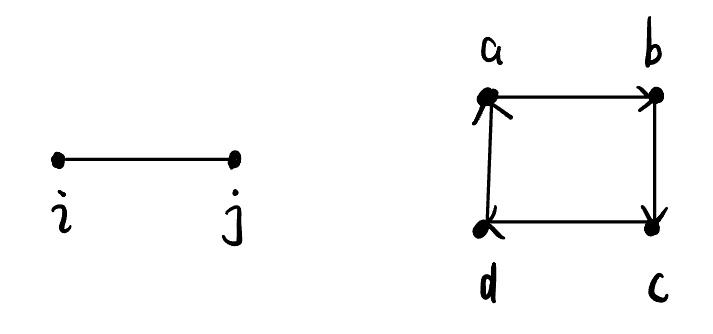
\includegraphics[width=0.35\linewidth]{./images/period-2.jpg}
        \caption{左：无向二部图；右：有向环}
        \label{srr-fig:period-1}
    \end{figure}

    举例：图 \ref{srr-fig:period-1}（左）中状态$i$的周期为$\textup{gcd}\{2,4,6,8,\dots\}=2$，因此$i$的周期为$2$；类似地，$j$的周期也为$2$。
        
    \begin{definition}[非周期性]
        \label{defn:aperiodicity}
        若状态$i$的周期为$1$，则状态$i$是非周期性的（aperiodic）。若马尔可夫链中所有的状态都是非周期性的，则这个马尔科夫链是非周期性的。
    \end{definition}

    \textbf{关于周期性的更多例子}
    \begin{itemize}
        \item 无向二部图中状态（即图中顶点）的周期为$2$，例如图 \ref{srr-fig:period-1}（左）；
        \item 长为$k>1$的有向环中点的周期为$k$，例如图 \ref{srr-fig:period-1}（右）；
        \item 周期性阻止概率分布收敛到单一极限分布：
        \begin{itemize}
            \item 例如图 \ref{srr-fig:period-1}（左）中初始状态为$i$的马尔科夫链，奇数步后在$j$，偶数步后在$i$，因此概率分布会在两个分布之间振荡，无法收敛到单一极限。
        \end{itemize}
    \end{itemize}

    \begin{proposition}[可达性结果（Reachability Result）]
        \label{proposition:re-re}
        在任意有限（状态集合有限）、不可约、非周期的马尔可夫链中，存在$\tau<\infty$满足对于所有的$i,j$和$t\ge \tau$有：
        \[
            \Pr[X_t=j\mid X_0=i]>0.
        \]
    \end{proposition}

    注意：仅仅有限、不可约这两个条件不能得出性质 \ref{proposition:re-re} 中的结果。例如针对图 \ref{srr-fig:period-1}（左），其满足有限和不可约，但在$t$为奇数时，$\Pr[X_t=i|X_0=i]=0$，在$t$为偶数时，$\Pr[X_t=j|X_0=i]=0$。即因为周期性，导致某些时刻概率恒为$0$，不满足性质 \ref{proposition:re-re} 中的结果，因此需要“非周期”这个条件。



    \subsubsection{马尔科夫链基本定理}
        
    \begin{definition}[稳态分布]
        \label{defn:stationary-distribution}
        一个概率向量$\vec{\pi}\in\mathbb{R}^n$对于$P$是稳态分布（stationary distribution），如果满足：$\vec{\pi}P=\vec{\pi}$。
    \end{definition}

    \begin{itemize}
        \item $\vec{\pi}$是$P$的左特征向量，对应的特征值为$1$；
        \item 如果$\vec{\pi}$是稳态分布，那么对于所有的$t>0$有$\vec{\pi}P^t=\vec{\pi}$：
        \begin{itemize}
            \item $\vec{\pi}P^t=\vec{\pi}P\cdot P^{t-1}=\vec{\pi}P^{t-1}=\vec{\pi}P\cdot P^{t-2}=\vec{\pi}P^{t-2}=\cdots=\vec{\pi}$。
        \end{itemize}
    \end{itemize}

    \begin{definition}[TV距离]
        \label{defn:tv-distance}
        两个概率分布$\vec{p},\vec{q}\in\mathbb{R}^n$之间的TV距离（total variation distance）定义为
        \[
            d_{\textup{TV}}(\vec{p},\vec{q}):=\frac{1}{2}\sum_{i=1}^n{|p(i)-q(i)|}=\frac{1}{2}\lVert \vec{p}-\vec{q}\rVert_1.
        \]
    \end{definition}

    如果在$t\rightarrow \infty$时有$d_{\textup{TV}}(\vec{p}_t,\vec{q})\rightarrow 0$，则称$\vec{p}_t$（定义 \ref{defn:probability-distribution}）收敛于$\vec{q}$。

    \begin{theorem}[马尔科夫链基本定理] 
        \label{thrm:fund-mc}
        令$P\in \mathbb{R}^{n\times n}$定义一个有限、不可约、非周期的马尔科夫链。则对任意的初始分布$\vec{p}_0$，其对应的$\vec{p}_t:=\vec{p}_0P^t$在$t\rightarrow \infty$时收敛于一个唯一的稳态分布$\vec{\pi}$。
    \end{theorem}

    定理 \ref{thrm:fund-mc} 针对所有满足有限、不可约、非周期的马尔科夫链成立，而无向图上的随机游走是特殊的马尔科夫链，接下来我们运用谱分析证明一个特殊版本（关于无向图上的随机游走）的马尔可夫链基本定理。


        
\subsection{无向图上的简单随机游走}
        
本节我们考虑无向图上的随机游走，这是一种特殊的马尔科夫链，希望运用谱图论证明定理 \ref{thrm:fund-mc}。

\textbf{一些基础符号。}针对无权无向图$G=(V,E)$，$A\in\mathbb{R}^{n\times n}$表示图$G$的邻接矩阵，$D\in\mathbb{R}^{n\times n}$表示度数对角矩阵，其中$D_{ii}=\textup{deg}(i)$。

\vspace{0.2cm}
回忆无权无向图$G=(V,E)$上的随机游走是指从图中某个点出发，在每一步，从当前所在点的邻居中均匀随机地选择一个点进行移动（游走）。
        
\begin{itemize}
    \item 令$P_{ij}$表示从点$i$到点$j$的单步转移概率，则：
    \begin{itemize}
        \item 若$(i,j)\in E$，有$P_{ij}=\frac{1}{\textup{deg}(i)}$；
        \item 若$(i,j)\notin E$，有$P_{ij}=0$；
    \end{itemize}
    \item 因此\textcolor{blue}{转移矩阵$P=D^{-1}A$}。这称为图上简单随机游走的转移矩阵。
    \item 令$\bm{p}_0:V\rightarrow \mathbb{R}$表示初始概率分布，则$\bm{p}_{t+1} = \bm{p}_t P= \bm{p}_t D^{-1}A
        \quad \Rightarrow \quad
        \textcolor{blue}{\bm{p}_t = \bm{p}_0 (D^{-1}A)^t}.$
\end{itemize}

\vspace{0.2cm}
类似定义 \ref{defn:stationary-distribution}，我们定义$\bm{\pi}:V\to \mathbb{R}$为稳态分布，如果$\bm{\pi}$满足$\bm{\pi}P=\bm{\pi}$。$\bm{\pi}$是$P$的左特征向量，对应的特征值为$1$。%针对$P=D^{-1}A$，一个自然的稳态分布$\bm{\pi}$可以定义为$\bm{\pi}(i)=\frac{\textup{deg}(i)}{2|E|}$。

\begin{lemma}
    \label{lemma:sta-dist-graoh}
    令$G=(V,E)$表示一个无向图，令$P=D^{-1}A$。对所有$i\in V$，定义
    \[
        \bm{\pi}(i)=\frac{\textup{deg}(i)}{2|E|},
    \]
    则$\bm{\pi}$是$P$的一个稳态分布。
            
    \begin{proof}
        \begin{align*}
            \bm{\pi}P&=\bm{\pi}D^{-1}A\\
            &=\frac{1}{2|E|}\vec{1}\cdot  A\\
            &=\frac{1}{2|E|}\left(\textup{deg}(1),\dots,\textup{deg}(n)\right)\\
            &=\bm{\pi}.
        \end{align*}
    \end{proof}
\end{lemma}

定理 \ref{thrm:fund-mc} 中马尔科夫链需要满足有限、不可约、非周期三个条件。因此我们需要在图上对应有限、不可约、非周期三个条件。

\paragraph{有限。}只要图上的顶点数$|V|$有限就满足了“有限”这个条件。

\paragraph{不可约。}若$G$是不连通的，则随机游走的长期表现（long-term behavior）取决于起始点，稳态分布也不是唯一的。
        
考虑图$G$中有两个连通分量$G_1=(V_1,E_1)$和$G_2=(V-V_1,E-E_1)$：
\begin{itemize}
    \item 若起始点为$G_1$中的点（即$V_1$中的点），则稳态分布为
    \begin{itemize}
        \item 对$i\in V_1$，$\bm{\pi}(i)=\frac{\textup{deg}(i)}{2|E_1|}$；
        \item 对$i\notin V_1$，$\bm{\pi}(i)=0$；
    \end{itemize}

    \item 若起始点为$G_2$中的点（即$V-V_1$中的点），则稳态分布为
    \begin{itemize}
        \item 对$i\notin V_1$，$\bm{\pi}(i)=\frac{\textup{deg}(i)}{2|E-E_1|}$；
        \item 对$i\in V_1$，$\bm{\pi}(i)=0$。
    \end{itemize}
\end{itemize}

\begin{fact}
    \label{fact:irre-graph}
    当且仅当$G$连通时，不可约条件满足。
\end{fact}

\paragraph{非周期。}即使在连通图中，随机游走也可能不会收敛到一个稳态分布，例如图 \ref{srr-fig:period-1} （左）中的连通二部图，其概率分布会在两个分布之间振荡，无法收敛到单一极限。

\begin{fact}
    \label{fact:aper-graph}
    当且仅当$G$是非二部图（non-bipartite）时，非周期条件满足。
\end{fact}



    \subsubsection{特殊的马尔科夫链基本定理}
        
    结合事实 \ref{fact:irre-graph}、事实 \ref{fact:aper-graph} 和引理 \ref{lemma:sta-dist-graoh}，我们想要证明的特殊版本的定理 \ref{thrm:fund-mc} 变为以下定理：

    \begin{theorem}
        \label{thrm:special-fund-mc}
        令$G$表示一个无向、连通的非二部图，并且转移矩阵$P=D^{-1}A$，则满足以下定义的分布$\bm{\pi}$是\textbf{唯一}的稳态分布：
        \[
            \bm{\pi}(i)=\frac{\textup{deg}(i)}{2|E|}.
        \]
        即对任意的初始分布$\bm{p}_0$，其对应的$\bm{p}_t=\bm{p}_0P^t$在$t\to \infty$时收敛于$\bm{\pi}$%，即$\bm{p}_t=\bm{p}_0P^t\to \bm{\pi}$
            。
    \end{theorem}
        


\subsection{\texorpdfstring{$d$}{d}-正则非二部图上的简单随机游走}

    接下来我们的目标是使用\textbf{谱分析（spectral analysis）}证明上节中给出的特殊的马尔可夫链基本定理（定理 \ref{thrm:special-fund-mc}），即证明随机游走会收敛到一个唯一的稳态分布。此外谱技巧（spectral techniques）可以精确分析混合时间（mixing time），即收敛速度。 本节首先考虑在一类特殊的图（$d$-正则非二分图）上进行证明，在后面章节推广到更一般的图上。

    对$d$-正则图：
    \begin{itemize}
        \item 简单随机游走的转移矩阵$P=D^{-1}A=\frac{1}{d}A=\mathcal{A}$；
        \begin{itemize}
            \item $\mathcal{A}$为正则化的邻接矩阵；
        \end{itemize}
        \item $P$为实对称矩阵，因此特征值都是实数；
        \item 稳态分布满足$\bm{\pi}(i)=\frac{d}{dn}=\frac{1}{n}$，因此$\bm{\pi}=\frac{\bm{1}}{n}$。
    \end{itemize}

    \vspace{0.2cm}
    \textbf{$P=\mathcal{A}$的谱性质。}令$\alpha_1\ge \alpha_2\ge \dots\ge \alpha_n$表示$\mathcal{A}$的特征值，对应的一组标准正交特征向量为$v_1,v_2,\dots,v_n$：
    \begin{itemize}
        \item 由Notes Lec 10中引理 28 可知，$\alpha_1=1$，且$v_1=\frac{\bm{1}}{\sqrt{n}}$；
        \item \textcolor{blue}{当且仅当$G$是连通图时，$\alpha_2<1$}；
            \begin{itemize}
                \item 由Notes Lec 10中引理 22 可知，当且仅当$G$是连通图时，$L=D-A$的第二小特征值$\lambda_2>0$（对应的特征向量为$v_2$），可以验证$\alpha_i=1-\frac{\lambda_i}{d}$，因此$\alpha_2=1-\frac{\lambda_2}{d}<1$；
            \end{itemize}
        \item \textcolor{blue}{当且仅当$G$是非二部图时，$\alpha_n>-1$}（当且仅当$G$是二部图时，$\alpha_n=-1$）；
            \begin{itemize}
                \item 由Notes Lec 10中引理 12 可得。
            \end{itemize}
        \end{itemize}

    \vspace{0.25cm}
    下面给出与定理 \ref{thrm:special-fund-mc} 相对应的$d$-正则非二部图上的结论，即定理 \ref{thrm:fund-mc-d-1}。
            
    \begin{theorem}
        \label{thrm:fund-mc-d-1}
        令$G$表示一个$d$-正则化的、无向、连通的非二部图，简单随机游走的转移矩阵$P=D^{-1}A=\mathcal{A}$，那么对于所有的初始概率分布$\bm{p}_0$：
        \[
            \lim_{t \to \infty} \bm{p}_0\mathcal{A}^t  = \frac{\bm{1}}{n}.
        \]
    \end{theorem}

    \begin{proof}
        % 因为$\mathcal{A}$的特征向量$v_1,\dots,v_n$构成一组标准正交基，因此任意的初始向量$\bm{p}_0$都可以用$v_1,\dots,v_n$表示，即$\bm{p}_0=\sum_{i=1}^n{c_iv_i^{\top}}$，其中$c_1,\dots,c_n$为常数。
                    
        % 此外，
        $\mathcal{A}$的特征分解可以表示为$\mathcal{A}=\sum_{i=1}^n{\alpha_iv_iv_i^{\top}}$。由于$v_1,\dots,v_n$构成一组标准正交基，则对任意$i\ne j$有$v_i^{\top}v_j=0$，对任意$i\in[n]$有$v_i^{\top}v_i=1$。因此$\mathcal{A}^t=\sum_{i=1}^n{\alpha_i^tv_iv_i^{\top}}$。

        \begin{align*}
            \bm{p}_0\mathcal{A}^t&=\bm{p}_0\sum_{i=1}^n{\alpha_i^tv_iv_i^{\top}}\\
            &=\bm{p}_0\cdot \alpha_1^tv_1v_1^{\top}+\bm{p}_0\sum_{i=2}^n{\alpha_i^tv_iv_i^{\top}}\\
            &=\frac{\bm{1}}{n}+\bm{p}_0\sum_{i=2}^n{\alpha_i^tv_iv_i^{\top}}&&\text{（$\alpha_1=1,v_1=\frac{\bm{1}}{\sqrt{n}}$且$\bm{p}_0$满足$\sum_{i=1}^n\bm{p}_0(i)=1$）}
        \end{align*}

        等式两边同时取极限，可得：
                    
        \begin{align*}
            \lim_t \bm{p}_0\mathcal{A}^t =\lim_t \frac{\bm{1}}{n}+\bm{p}_0\sum_{i=2}^n{\alpha_i^tv_iv_i^{\top}}=\frac{\bm{1}}{n},
        \end{align*}
        
        这是因为在连通的非二部图中，$1>\alpha_2\ge \alpha_3\ge \dots\ge \alpha_n>-1$，因此在$t\to \infty$时，$\forall i>1$，${|\alpha_i^t|}\to 0$，即$\bm{p}_0\sum_{i=2}^n{\alpha_i^tv_iv_i^{\top}}\to 0$。
                    
    \end{proof}

    马尔科夫链基本定理表明在步数$t\to \infty$时，随机游走的概率分布趋于稳态分布。现在我们关心$t$足够大时，随机游走概率分布的表现，而不是$t\to \infty$时。因此我们引入混合时间（mixing time）的概念。

    \begin{definition}[混合时间]
        \label{defn:mixing-time}
        对于转移矩阵为$P$的随机游走，令$\bm{p}_t=\bm{p}_0P^t$表示从初始分布$\bm{p}_0$开始的步长为$t$的随机游走的概率分布，$\bm{\pi}=\lim_{t \to \infty} \bm{p}_t$表示稳态分布。混合时间$\tau_{\varepsilon}(P)$定义为对任意初始分布$\bm{p}_0$，满足$d_{\textup{TV}}(\bm{p}_t,\bm{\pi})\le \varepsilon$的最小的步数$t$。
    \end{definition}

    在本节中，除非$\varepsilon$被特殊指明，否则我们默认$\varepsilon=1/4$。接下来我们给出简单随机游走混合时间的上界。%与上节类似，我们首先在一类特殊的图（$d$-正则图）上给出混合时间的上界（更简单），其次在更一般的图上给出混合时间的上界。

    回忆在$d$-正则图上，$P=D^{-1}A=\frac{1}{d}A=\mathcal{A}$，$W=\frac{1}{2}I+\frac{1}{2}P=\frac{1}{2}I+\frac{1}{2}\mathcal{A}$。$1=\alpha_1\ge \alpha_2\ge\dots \ge \alpha_n\ge -1$表示$\mathcal{A}$的特征值，对应的一组标准正交的特征向量为$v_1,\dots,v_n$。稳态分布为$\bm{\pi}=\frac{\bm{1}}{n}$。

    定义\textbf{谱间隔（spectral gap）}为$g:=\min\{1-\alpha_2,1-|\alpha_n|\}$。

    \paragraph{通过谱间隔给出混合时间的上界：}

    \begin{fact}
        \label{fact:norm}
        对任意向量$x\in\mathbb{R}^n$，有$\lVert x\rVert_1\le \sqrt{n}\lVert x\rVert_2$。
        \begin{proof}
            利用柯西不等式：
            \begin{align*}
                \lVert x\rVert_1=\sum_{i=1}^n{|x(i)|}
                \le \sqrt{\left(\sum_{i=1}^n{1^2}\right)\left(\sum_{i=1}^n{x(i)^2}\right)}
                =\sqrt{n}\cdot \lVert x\rVert_2.
            \end{align*}
        \end{proof}
    \end{fact}
                
    \begin{theorem}
        \label{thrm:mixing-time-d-sg}
        令$G$表示一个无向、连通、非二部图的$d$-正则图，$P=\mathcal{A}$为图上的简单随机游走转移矩阵。则$\tau_{\varepsilon}(P)\lesssim\frac{1}{g}\ln{\left(\frac{n}{\varepsilon}\right)}$。
    \end{theorem}

    注：$a \lesssim b$中$\lesssim$符号隐藏了常数，表示$a\le c\cdot b$，其中$c$是一个常数。可以认为$\lesssim$符号与$O$符号类似。

    定理 \ref{thrm:mixing-time-d-sg} 表明无向、连通、非二部图（连通的非二部图的$g>0$）的$d$-正则图上简单随机游走的混合时间与谱间隔$g$有关。

    \begin{proof}
        因为$\mathcal{A}$的特征向量$v_1,\dots,v_n$（列向量）构成一组标准正交基，因此任意的初始向量$\bm{p}_0$（行向量）都可以用$v_1,\dots,v_n$表示，即$\bm{p}_0=\sum_{i=1}^n{c_iv_i^{\top}}$，其中$c_1,\dots,c_n$为常数。此外，$P=\mathcal{A}=\sum_{i=1}^n{\alpha_iv_iv_i^{\top}}$，且$P^t=\mathcal{A}^t=\sum_{i=1}^n{\alpha_i^tv_iv_i^{\top}}$。%则$\bm{p}_t=\bm{p}_0P^t=\sum_{i=1}^n{c_i\alpha_i^tv_i^{\top}}$。
        
        由定理 \ref{thrm:fund-mc-d-1} 的证明可知$\bm{p}_t=\bm{p}_0P^t=\frac{\bm{1}}{n}+\bm{p}_0\sum_{i=2}^n{\alpha_i^tv_iv_i^{\top}}$，因此
                    
        \begin{align*}
            d_{\textup{TV}}(\bm{p}_t,\bm{\pi})&=\frac{1}{2}\lVert \bm{p}_t-\bm{\pi} \rVert_1\\
            % &\le \lVert \bm{p}_t-\bm{\pi} \rVert_1\\
            &=\frac{1}{2}\lVert \frac{\bm{1}}{n}+\bm{p}_0\sum_{i=2}^n{\alpha_i^tv_iv_i^{\top}}-\frac{\bm{1}}{n}\rVert_1\\
            &=\frac{1}{2}\lVert \bm{p}_0\sum_{i=2}^n{\alpha_i^tv_iv_i^{\top}}\rVert_1\\
            &=\frac{1}{2}\lVert \sum_{i=2}^n{c_i\alpha_i^tv_i^{\top}}\rVert_1&&\text{($\bm{p}_0=\sum_{i=1}^n{c_iv_i^{\top}}$)}\\
            &\le \frac{\sqrt{n}}{2}\lVert \sum_{i=2}^n{c_i\alpha_i^tv_i^{\top}}\rVert_2&&\text{（事实 \ref{fact:norm}）}.
        \end{align*}

        令向量$X=\sum_{i=2}^n{c_i\alpha_i^tv_i^{\top}}$，则$X(k)=\sum_{i=2}^n{c_i\alpha_i^tv_i(k)}$，因此
        
        \begin{align*}
            \lVert \sum_{i=2}^n{c_i\alpha_i^tv_i^{\top}}\rVert_2^2&=\lVert X\rVert_2^2\\
            &=\sum_{k=1}^n{X(k)^2}\\
            &=\sum_{k=1}^n{\left(\sum_{i=2}^n{c_i\alpha_i^tv_i(k)}\right)^2}\\
            &=\sum_{k=1}^n{\left(\sum_{i=2}^n{\sum_{j=2}^n{c_i\alpha_i^tv_i(k)\cdot c_j\alpha_j^tv_j(k)}}\right)}\\
            &=\sum_{i=2}^n{\sum_{j=2}^n{c_i\alpha_i^tc_j\alpha_j^t\sum_{k=1}^n{v_i(k)v_j(k)}}}\\
            &=\sum_{i=2}^n{c_i^2\alpha_i^{2t}}&&\text{（$v_1,\dots,v_n$是一组标准正交基）}\\
            &\le (1-g)^{2t}\sum_{i=2}^n{c_i^2}\\
            &\le e^{-2gt}\sum_{i=2}^n{c_i^2}.
        \end{align*}

        结合上面两个式子，有：
        
        \begin{align*}
            d_{\textup{TV}}(\bm{p}_t,\bm{\pi})&\le \frac{\sqrt{n}}{2}\lVert \sum_{i=2}^n{c_i\alpha_i^tv_i^{\top}}\rVert_2\\
            &\le\frac{\sqrt{n}}{2}\sqrt{e^{-2gt}\sum_{i=2}^n{c_i^2}}\\
            &\le\frac{\sqrt{n}}{2}\sqrt{e^{-2gt}\sum_{i=1}^n{c_i^2}}\\
            &=\frac{\sqrt{n}}{2}\sqrt{e^{-2gt}\left\|p_0\right\|_2^2}\\
            &\le\frac{\sqrt{n}}{2}\sqrt{e^{-2gt}\left\|p_0\right\|_1}\\
            &=\frac{\sqrt{n}}{2}e^{-gt}\\
            &=\frac{\sqrt{n}}{2}e^{-g\cdot C\frac{1}{g}\ln{\left(\frac{n}{\varepsilon}\right)}}&&\text{（$t=\tau_{\varepsilon}(P)\lesssim\frac{1}{g}\ln{\left(\frac{n}{\varepsilon}\right)}$）}\\
            &=\frac{\sqrt{n}}{2}\left(\frac{\varepsilon}{n}\right)^{C}\\
            &\le \varepsilon.&&\text{（取足够大的$C\ge 1$）}\\
            %&\lesssim \sqrt{n}e^{-tg}.
        \end{align*}
    \end{proof}

    

            
\subsection{\texorpdfstring{$d$}{d}-正则图上的懒惰随机游走}

\paragraph{去掉非周期性条件。}定理 \ref{thrm:special-fund-mc} 中的非二部图保证了马尔可夫链是非周期的（事实 \ref{fact:aper-graph}）。若想移除非二部图这个条件，我们可以给图上的点加自环（self-loops）。这将引出懒惰随机游走（lazy random walk）的概念。本节中我们首先研究$d$-正则非二分图上的懒惰随机游走。

\begin{definition}[（$d$-正则图上的）懒惰随机游走]
    \label{defn:lazy-random-walk}
    给定一个$d$-正则无向图$G$，其上的懒惰随机游走对应的转移矩阵$W$定义为：\[W=\frac{1}{2}I+\frac{A}{2d}.\]
\end{definition}

直观上看，图上的懒惰随机游走从某个点开始，在每一步，以$\frac{1}{2}$的概率留在原地，以$\frac{1}{2}$的概率随机均匀随机地选择一个邻居进行转移（游走）。

考虑懒惰随机游走的好处：
\begin{itemize}
    \item 加自环打破了二部图的周期性；
    \item 这种修改确保马尔可夫链变为非周期性的，同时不会显著改变图的结构。
\end{itemize}

\iffalse
\begin{corollary}
    \label{coro:fund-mc-lazy}
    令$G$表示一个无向、连通图。令$W=\frac{1}{2}I+\frac{1}{2}D^{-1}A$表示懒惰随机游走的转移矩阵。则满足以下定义的分布$\bm{\pi}$是\textbf{唯一}的稳态分布：
    \[
        \bm{\pi}(i)=\frac{\textup{deg}(i)}{2|E|}.
    \]
    即对任意的初始分布$\bm{p}_0$，其对应的$\bm{p}_t=\bm{p}_0W^t$在$t\to \infty$时收敛于$\bm{\pi}$%，即$\bm{p}_t=\bm{p}_0W^t\to \bm{\pi}$
    。
\end{corollary}
\fi

首先分析懒惰随机游走转移矩阵$W$的谱性质。
            
\vspace{0.2cm}
\textbf{$W$的谱性质。}由$W=\frac{1}{2}I+\frac{1}{2}\mathcal{A}$可知，$W$的特征值为$\frac{1}{2}(1+\alpha_i)$，对应的特征向量为$v_i$。$W$的特征值$\frac{1}{2}(1+\alpha_i)$有以下规律：
\begin{itemize}
    \item $W$的最大特征值为$\frac{1}{2}(1+\alpha_1)=1$；
    \item 因为$\alpha_i\ge -1$，因此对所有$i\in[n]$，$W$的特征值$\frac{1}{2}(1+\alpha_i)\ge 0$；
    \item $1> \frac{1+\alpha_2}{2}\ge \dots\ge \frac{1+\alpha_n}{2}\ge 0$。
\end{itemize}
            
下面给出$d$-正则非二分图上的稳态分布，即定理 \ref{thrm:fund-mc-d-2}。

\begin{theorem}
    \label{thrm:fund-mc-d-2}
    令$G$表示一个$d$-正则化的、无向、连通图，转移矩阵$W=\frac{1}{2}I+\frac{1}{2}\mathcal{A}$，那么对于所有的初始概率分布$\bm{p}_0$：
    \[
        \lim_{t \to \infty} \bm{p}_0W^t  = \frac{\bm{1}}{n}.
    \]
\end{theorem}

\begin{proof}
    （证明与定理 \ref{thrm:fund-mc-d-1} 类似。）由$W$的谱性质可知，$W$的特征值为$\frac{1}{2}(1+\alpha_i)$，对应的特征向量为$v_i$，因此$W$的特征分解可以表示为$W=\sum_{i=1}^n{\frac{1+\alpha_i}{2}v_iv_i^{\top}}$，类似地，$W^t=\sum_{i=1}^n{\left(\frac{1+\alpha_i}{2}\right)^tv_iv_i^{\top}}$。
    \begin{align*}
        \bm{p}_0W^t&=\bm{p}_0\sum_{i=1}^n{\left(\frac{1+\alpha_i}{2}\right)^tv_iv_i^{\top}}\\
        &=\bm{p}_0\left(\frac{1+\alpha_1}{2}\right)v_1v_1^{\top}+\bm{p}_0\sum_{i=2}^n{\left(\frac{1+\alpha_i}{2}\right)^tv_iv_i^{\top}}\\
        &=\frac{\bm{1}}{n}+\bm{p}_0\sum_{i=2}^n{\left(\frac{1+\alpha_i}{2}\right)^tv_iv_i^{\top}}&&\text{（$\alpha_1=1,v_1=\frac{\bm{1}}{\sqrt{n}}$且$\bm{p}_0$满足$\sum_{i=1}^n\bm{p}_0(i)=1$）}
    \end{align*}

    等式两边同时取极限，可得：
    \begin{align*}
        \lim_t \bm{p}_0W^t =\lim_t \left(\frac{\bm{1}}{n}+\bm{p}_0\sum_{i=2}^n{\left(\frac{1+\alpha_i}{2}\right)^tv_iv_i^{\top}}\right)=\frac{\bm{1}}{n},
    \end{align*}
    
    这是因为在连通图中，$1>\alpha_2\ge \alpha_3\ge \dots\ge \alpha_n>-1$，因此$1> \frac{1+\alpha_2}{2}\ge \dots\ge \frac{1+\alpha_n}{2}\ge 0$。则在$t\to \infty$时，$\forall i>1$，${|\left(\frac{1+\alpha_i}{2}\right)^t|}\to 0$，即$\bm{p}_0\sum_{i=2}^n{\left(\frac{1+\alpha_i}{2}\right)^tv_iv_i^{\top}}\to 0$。
\end{proof}

\paragraph{通过导率（conductance）给出混合时间的上界：}
                
回忆在$d$-正则图上，懒惰随机游走的转移矩阵$W=\frac{1}{2}I+\frac{1}{2}P=\frac{1}{2}I+\frac{1}{2}\mathcal{A}$，$W$的特征值为$\frac{1}{2}(1+\alpha_i)$，均$\ge 0$。稳态分布为$\bm{\pi}=\frac{\bm{1}}{n}$。此外，图$G$的正则化拉普拉斯矩阵$\mathcal{L}=I-\frac{A}{d}=I-\mathcal{A}$，特征值为$0\le\lambda_1\le \lambda_2\le\dots\le \lambda_n\le 2$（对应的特征向量为$v_1,\dots,v_n$），其中$\lambda_i=1-\alpha_i$。

定义\textbf{谱间隔（spectral gap）}为$g:=\frac{1}{2}(1-\alpha_2)=\frac{1}{2}\lambda_2$。

\begin{theorem}
    \label{thrm:mixing-time-d-c}
    令$G$表示一个无向、连通的$d$-正则图，$W=\frac{1}{2}I+\frac{1}{2}\mathcal{A}$为图上的懒惰随机游走转移矩阵。则$\tau_{\varepsilon}(W)\lesssim\frac{1}{\phi(G)^2}\ln{\left(\frac{n}{\varepsilon}\right)}$。
\end{theorem}

定理 \ref{thrm:mixing-time-d-c} 表明无向、连通（连通图的$g>0$，即$\phi(G)>0$）的$d$-正则图上懒惰随机游走的混合时间与导率$\phi(G)$有关。

\begin{proof}
    （总体证明思路与定理 \ref{thrm:mixing-time-d-sg} 的证明类似，最后用到Cheeger不等式。）

    由定理 \ref{thrm:fund-mc-d-2} 的证明可知$\bm{p}_t=\bm{p}_0W^t=\frac{\bm{1}}{n}+\bm{p}_0\sum_{i=2}^n{\left(\frac{1+\alpha_i}{2}\right)^tv_iv_i^{\top}}$，因此

    \[
        d_{\textup{TV}}(\bm{p}_t,\bm{\pi})\le \frac{\sqrt{n}}{2}\lVert \sum_{i=2}^n{c_i\left(\frac{1+\alpha_i}{2}\right)^tv_i^{\top}}\rVert_2.
    \]
                    % \begin{align*}
                    %     d_{\textup{TV}}(\bm{p}_t,\bm{\pi})&=\frac{1}{2}\lVert \bm{p}_t-\bm{\pi} \rVert_1\\
                    %     % &\le \lVert \bm{p}_t-\bm{\pi} \rVert_1\\
                    %     &=\frac{1}{2}\lVert \frac{\bm{1}}{n}+\bm{p}_0\sum_{i=2}^n{\left(\frac{1+\alpha_i}{2}\right)^tv_iv_i^{\top}}-\frac{\bm{1}}{n}\rVert_1\\
                    %     &=\frac{1}{2}\lVert \bm{p}_0\sum_{i=2}^n{\left(\frac{1+\alpha_i}{2}\right)^tv_iv_i^{\top}}\rVert_1\\
                    %     &=\frac{1}{2}\lVert \sum_{i=2}^n{c_i\left(\frac{1+\alpha_i}{2}\right)^tv_i^{\top}}\rVert_1&&\text{($\bm{p}_0=\sum_{i=1}^n{c_iv_i^{\top}}$)}\\
                    %     &\le \frac{\sqrt{n}}{2}\lVert \sum_{i=2}^n{c_i\left(\frac{1+\alpha_i}{2}\right)^tv_i^{\top}}\rVert_2&&\text{（事实 \ref{fact:norm}）}.
                    % \end{align*}

    此外，
    
    \begin{align*}
        \lVert \sum_{i=2}^n{c_i\left(\frac{1+\alpha_i}{2}\right)^tv_i^{\top}}\rVert_2^2&=\sum_{i=2}^n{c_i^2\left(\frac{1+\alpha_i}{2}\right)^{2t}}\\
        &=\sum_{i=2}^n{c_i^2\left(1-\frac{\lambda_i}{2}\right)^{2t}}&&\text{（$\lambda_i=1-\alpha_i$）}\\
        &\le (1-g)^{2t}\sum_{i=1}^n{c_i^2}\\
        &\le e^{-2gt}\sum_{i=2}^n{c_i^2}.
    \end{align*}
                    % 令向量$X=\sum_{i=2}^n{c_i\left(\frac{1+\alpha_i}{2}\right)^tv_i^{\top}}$，则$X(k)=\sum_{i=2}^n{c_i\left(\frac{1+\alpha_i}{2}\right)^tv_i(k)}$，因此
                    % \begin{align*}
                    %     \lVert \sum_{i=2}^n{c_i\left(\frac{1+\alpha_i}{2}\right)^tv_i^{\top}}\rVert_2^2&=\lVert X\rVert_2^2\\
                    %     &=\sum_{k=1}^n{X(k)^2}\\
                    %     &=\sum_{k=1}^n{\left(\sum_{i=2}^n{c_i\left(\frac{1+\alpha_i}{2}\right)^tv_i(k)}\right)^2}\\
                    %     &=\sum_{k=1}^n{\left(\sum_{i=2}^n{\sum_{j=2}^n{c_i\left(\frac{1+\alpha_i}{2}\right)^tv_i(k)\cdot c_j\left(\frac{1+\alpha_j}{2}\right)^tv_j(k)}}\right)}\\
                    %     &=\sum_{i=2}^n{\sum_{j=2}^n{c_i\left(\frac{1+\alpha_i}{2}\right)^tc_j\left(\frac{1+\alpha_j}{2}\right)^t\sum_{k=1}^n{v_i(k)v_j(k)}}}\\
                    %     &=\sum_{i=2}^n{c_i^2\left(\frac{1+\alpha_i}{2}\right)^{2t}}&&\text{（$v_1,\dots,v_n$是一组标准正交基）}\\
                    %     &\le (1-g)^{2t}\sum_{i=2}^n{c_i^2}\\
                    %     &\le e^{-2gt}\sum_{i=2}^n{c_i^2}.
                    % \end{align*}

    结合上面两个式子，有：
    
    \begin{align*}
        d_{\textup{TV}}(\bm{p}_t,\bm{\pi})&\le \frac{\sqrt{n}}{2}\lVert \sum_{i=2}^n{c_i\left(\frac{1+\alpha_i}{2}\right)^tv_i^{\top}}\rVert_2\\
        &\le\frac{\sqrt{n}}{2}\sqrt{e^{-2gt}\sum_{i=2}^n{c_i^2}}\\
        &\le\frac{\sqrt{n}}{2}\sqrt{e^{-2gt}\sum_{i=1}^n{c_i^2}}\\
            &=\frac{\sqrt{n}}{2}\sqrt{e^{-2gt}\left\|p_0\right\|_2^2}\\
            &\le\frac{\sqrt{n}}{2}\sqrt{e^{-2gt}\left\|p_0\right\|_1}\\
            &=\frac{\sqrt{n}}{2}e^{-gt}\\
            &=\frac{\sqrt{n}}{2}e^{-g\cdot C\frac{1}{g}\ln{\left(\frac{n}{\varepsilon}\right)}}&&\text{（$t=\tau_{\varepsilon}(P)\lesssim\frac{1}{g}\ln{\left(\frac{n}{\varepsilon}\right)}$）}\\
            &=\frac{\sqrt{n}}{2}\left(\frac{\varepsilon}{n}\right)^{C}\\
            &\le \varepsilon.&&\text{（取足够大的$C\ge 1$）}\\
        %&\lesssim \sqrt{n}e^{-tg}.
    \end{align*}
                    
    由Notes Lec 14中的Cheeger不等式可知$\frac{\lambda_2}{2}\le \phi(G)\le \sqrt{2\lambda_2}$，因此$\lambda_2\ge \frac{\phi(G)^2}{2}$，$g=\frac{1}{2}\lambda_2\ge \frac{\phi(G)^2}{4}$，因此$\tau_{\varepsilon}(W)\le C_2\frac{1}{g}\ln{\left(\frac{n}{\varepsilon}\right)}\le 4C_2 \frac{1}{\phi(G)^2}\ln{\left(\frac{n}{\varepsilon}\right)}$，即$\tau_{\varepsilon}(W)\lesssim  \frac{1}{\phi(G)^2}\ln{\left(\frac{n}{\varepsilon}\right)}$。
\end{proof}

\textbf{应用：}对于扩展图（expanders）$G$，其导率满足$\phi(G)=\Omega(1)$，根据定理 \ref{thrm:mixing-time-d-c}，扩展图上的混合时间为$\tau_{\varepsilon}(W)=O(\log n)$，这一结论在以下场景下有用：
    \begin{itemize}
        \item 均匀采样；
        \item 设计随机化算法（randomized algorithms）；
        \item 快速混合马尔科夫链。
    \end{itemize}

总结：通过给图加自环、分析新图上懒惰随机游走可以简化分析。此外，加自环不会显著影响图上随机游走的性质。

            


\subsection{一般非二部图上的简单随机游走}

本节我们首先证明一般图上的马尔科夫链基本定理。其次给出一般图上的混合时间的上界。我们依然首先关心非二部图的情况。

\vspace{0.2cm}
对一般图：
\begin{itemize}
    \item 简单随机游走的转移矩阵$P=D^{-1}A$；
    \item 由于图不一定是$d$-正则图，因此$P$不一定是对称矩阵；
    \begin{itemize}
        \item 因此，谱定理（Notes Lec 10中的定理3）无法直接应用。
    \end{itemize}
\end{itemize}

\vspace{0.2cm}
\textbf{谱的相似性（spectral similarity）：}两个矩阵在谱性质上相似通常指它们的特征值/特征向量可以通过某种方式一一对应，且谱性质相近。如果两个矩阵$M,N$相似，即存在可逆矩阵$S$满足$M=S^{-1}NS$，则$M,N$具有相同的特征值（但特征向量可能不同）。
            
\vspace{0.2cm}
定义正则化邻接矩阵$\mathcal{A}=D^{-1/2}AD^{-1/2}$，可以验证$\mathcal{A}$一定为实对称矩阵。此时：
\begin{itemize}
    \item $P=D^{-1}A=D^{-1/2}\mathcal{A}D^{1/2}$，与$\mathcal{A}$相似，记为$P\sim \mathcal{A}$
    \item 根据谱的相似性，$P$的特征值与$\mathcal{A}$的特征值相同，均为实数。
\end{itemize}

\begin{lemma}
    \label{lemma:s-s}
    令$G$表示一个连通的无向图，其正则化邻接矩阵为$\mathcal{A}$。令$\alpha_1>\alpha_2\ge \dots\ge \alpha_n$表示$\mathcal{A}$的特征值，对应的一组标准正交特征向量为$v_1,\dots,v_n$，其中$v_1=\frac{1}{\sqrt{2|E|}}D^{1/2}\bm{1}$。
    则：
    \begin{itemize}
        \item $P=D^{-1}A$的特征值为$\alpha_1,\dots,\alpha_n$；
        \item $P$的特征向量为$D^{-1/2}v_1,\dots,D^{-1/2}v_n$。
    \end{itemize}
\end{lemma}

\begin{proof}
    利用谱的相似性依次证明：
    \begin{itemize}
        \item 由于$P\sim \mathcal{A}$，因此$P$与$\mathcal{A}$的特征值相同，为$\alpha_1,\dots,\alpha_n$；
        \item $PD^{-1/2}v_i=D^{-1/2}\mathcal{A}D^{1/2}D^{-1/2}v_i=D^{-1/2}\mathcal{A}v_i=D^{-1/2}\alpha_iv_i=\alpha_iD^{-1/2}v_i$。
    \end{itemize}
\end{proof}

注意$v_1,\dots,v_n$是一组标准正交基，即对于任意$i\ne j\in[n]$，有$\langle v_i,v_j\rangle=0$；对于任意$i\in[n]$，有$\lVert v_i\rVert_2=\sqrt{v_i^{\top}v_i} =1$。但$P$的特征向量$D^{-1/2}v_1,\dots,D^{-1/2}v_n$不一定是一组标准正交基。因此，我们定义带权重的内积：
\begin{itemize}
    \item $\langle u,v\rangle_{D}=u^{\top}Dv$；
    \item $\lVert v\rVert_{D}=\sqrt{v^{\top}Dv}$。
\end{itemize}

在带权重内积的度量下，$P$的特征向量$D^{-1/2}v_1,\dots,D^{-1/2}v_n$是一组标准正交基，即：
\begin{itemize}
    \item 对于任意$i\ne j\in[n]$，有$\langle D^{-1/2}v_i,D^{-1/2}v_j\rangle_D=0$；
    \item 对于任意$i\in[n]$，有$\Vert D^{-1/2}v_i\rVert_D =1$。
\end{itemize}

\vspace{0.25cm}
下面给出与定理 \ref{thrm:special-fund-mc}、定理 \ref{thrm:fund-mc-d-1} 相对应的一般图上的结论，即定理 \ref{thrm:fund-mc-g-1}。
            
\begin{theorem}
    \label{thrm:fund-mc-g-1}
    令$G$表示一个无向、连通的非二部图，简单随机游走的转移矩阵$P=D^{-1}A=D^{-1/2}\mathcal{A}D^{1/2}$，特征值为$1=\alpha_1>\alpha_2\ge\dots \ge \alpha_n> -1$。那么对于所有的初始概率分布$\bm{p}_0$：
    \[
        \lim_{t \to \infty} \bm{p}_0P^t  = \frac{\bm{d}}{2|E|},
    \]
    其中$\bm{d}\in \mathbb{R}^n,\bm{d}(i)=\textup{deg}(i)$。
\end{theorem}
                
\begin{proof}
    % 因为$\mathcal{A}$的特征向量$v_1,\dots,v_n$构成一组标准正交基，因此任意的初始向量$\bm{p}_0$都可以用$v_1,\dots,v_n$表示，即$\bm{p}_0=\sum_{i=1}^n{c_iv_i^{\top}}$，其中$c_1,\dots,c_n$为常数。
                    
    % 此外，
    因为$P=D^{-1/2}\mathcal{A}D^{1/2}$，因此$P^t=D^{-1/2}\mathcal{A}^tD^{1/2}$。此外，$\mathcal{A}$的特征分解可以表示为$\mathcal{A}=\sum_{i=1}^n{\alpha_iv_iv_i^{\top}}$，$\mathcal{A}^t=\sum_{i=1}^n{\alpha_i^tv_iv_i^{\top}}$，因此$P^t=D^{-1/2}\left(\sum_{i=1}^n{\alpha_i^tv_iv_i^{\top}}\right)D^{1/2}$。
                    
    \begin{align*}
        \bm{p}_0P^t&=\bm{p}_0D^{-1/2}\left(\sum_{i=1}^n{\alpha_i^tv_iv_i^{\top}}\right)D^{1/2}\\
        &=\bm{p}_0\cdot D^{-1/2}\alpha_1^tv_1v_1^{\top}D^{1/2}+\bm{p}_0D^{-1/2}\left(\sum_{i=2}^n{\alpha_i^tv_iv_i^{\top}}\right)D^{1/2}\\
        &=\frac{\bm{d}}{2|E|}+\bm{p}_0D^{-1/2}\left(\sum_{i=2}^n{\alpha_i^tv_iv_i^{\top}}\right)D^{1/2}&&\text{（$\alpha_1=1,v_1=\frac{1}{\sqrt{2|E|}}D^{1/2}\bm{1}$且$\sum_{i=1}^n\bm{p}_0(i)=1$）}
    \end{align*}

    等式两边同时取极限，可得：
                    
    \begin{align*}
        \lim_t \bm{p}_0P^t =\lim_t \left(\frac{\bm{d}}{2|E|}+\bm{p}_0D^{-1/2}\left(\sum_{i=2}^n{\alpha_i^tv_iv_i^{\top}}\right)D^{1/2}\right)=\frac{\bm{d}}{2|E|},
    \end{align*}

    这是因为在连通的非二部图中，$1>\alpha_2\ge \alpha_3\ge \dots\ge \alpha_n>-1$，因此在$t\to \infty$时，$\forall i>1$，${|\alpha_i^t|}\to 0$，即$\bm{p}_0D^{-1/2}\left(\sum_{i=2}^n{\alpha_i^tv_iv_i^{\top}}\right)D^{1/2}\to 0$。
\end{proof}

定义\textbf{谱间隔（spectral gap）}为$g:=\min\{1-\alpha_2,1-|\alpha_n|\}$。

\paragraph{通过谱间隔给出混合时间的上界：}

\begin{theorem}
    \label{thrm:mixing-time-g-sg}
    令$G$表示一个无向、连通的非二部图，$P=D^{-1}A=D^{-1/2}\mathcal{A}D^{1/2}$为图上的简单随机游走转移矩阵。则$\tau_{\varepsilon}(P)\lesssim\frac{1}{g}\ln{\left(\frac{n}{\varepsilon}\right)}$。对于带权的无向、连通、非二部图，$\tau_{\varepsilon}(P)\lesssim\frac{1}{g}\ln{\left(\frac{n}{\varepsilon\cdot \bm{\pi}_{\textup{min}}}\right)}$，其中$\bm{\pi}_{\textup{min}}=\min_{i\in[n]}{\bm{\pi}(i)}=\min_{i\in [n]}{\frac{\textup{deg}(i)}{2|E|}}$。



                % \begin{proof}
                %     因为$\mathcal{A}$的特征向量$v_1,\dots,v_n$（列向量）构成一组标准正交基，因此任意的初始向量$\bm{p}_0$（行向量）都可以用$v_1,\dots,v_n$表示，即$\bm{p}_0=\sum_{i=1}^n{c_iv_i^{\top}}$，其中$c_1,\dots,c_n$为常数。此外，由定理 \ref{thrm:fund-mc-g-1} 的证明可知$\bm{p}_t=\bm{p}_0P^t=\frac{\bm{d}}{2|E|}+\bm{p}_0D^{-1/2}\left(\sum_{i=2}^n{\alpha_i^tv_iv_i^{\top}}\right)D^{1/2}$。

                %     \begin{align*}
                %         d_{\textup{TV}}(\bm{p}_t,\bm{\pi})&=\frac{1}{2}\lVert \bm{p}_t-\bm{\pi} \rVert_1\le \lVert \bm{p}_t-\bm{\pi} \rVert_1\\
                %         % &\le \lVert \bm{p}_t-\bm{\pi} \rVert_1\\
                %         % &=\frac{1}{2}\lVert \frac{\bm{1}}{n}+\bm{p}_0\sum_{i=2}^n{\alpha_i^tv_iv_i^{\top}}-\frac{\bm{1}}{n}\rVert_1\\
                %         &=\lVert \bm{p}_0D^{-1/2}\left(\sum_{i=2}^n{\alpha_i^tv_iv_i^{\top}}\right)D^{1/2}\rVert_1\\
                %         &=\lVert \sum_{i=2}^n{c_i\alpha_i^tv_i^{\top}}\rVert_1&&\text{($\bm{p}_0=\sum_{i=1}^n{c_iv_i^{\top}}$)}\\
                %         &\le \frac{\sqrt{n}}{2}\lVert \sum_{i=2}^n{c_i\alpha_i^tv_i^{\top}}\rVert_2&&\text{（事实 \ref{fact:norm}）}.
                %     \end{align*}
                    
                % \end{proof}
            \end{theorem}       

    


\subsection{一般图上的懒惰随机游走}

在最后一节中，我们来研究一般图上的随机游走。与1.4节类似，为了满足非周期性条件，我们定义一般图上的懒惰随机游走：

\begin{definition}[懒惰随机游走]
    \label{defn:lazy-random-walk-general}
    给定一个无向图$G$，其上的懒惰随机游走对应的转移矩阵$W$定义为：\[W=\frac{1}{2}I+\frac{1}{2}D^{-1}A.\]
\end{definition}

与非二部图的情况类似，这里利用正则化邻接矩阵$\mathcal{A}=D^{-1/2}AD^{-1/2}$，可以得到：
\begin{itemize}
    \item $W=\frac{1}{2}I+\frac{1}{2}P=D^{-1/2}(\frac{1}{2}I+\frac{1}{2}\mathcal{A})D^{1/2}$，与$\frac{1}{2}I+\frac{1}{2}\mathcal{A}$相似，记为$W\sim \frac{1}{2}I+\frac{1}{2}\mathcal{A}$；
    \item 根据谱的相似性，$W$的特征值与$\frac{1}{2}I+\frac{1}{2}\mathcal{A}$的特征值相同，均为实数。
\end{itemize}

\begin{lemma}
    \label{lemma:s-s-general}
    令$G$表示一个连通的无向图，其正则化邻接矩阵为$\mathcal{A}$。令$\alpha_1>\alpha_2\ge \dots\ge \alpha_n$表示$\mathcal{A}$的特征值，对应的一组标准正交特征向量为$v_1,\dots,v_n$，其中$v_1=\frac{1}{\sqrt{2|E|}}D^{1/2}\bm{1}$。
    则：
    \begin{itemize}
        \item $W$的特征值为$\frac{1+\alpha_i}{2}$；
        \item $W$的特征向量也为$D^{-1/2}v_1,\dots,D^{-1/2}v_n$。
    \end{itemize}
\end{lemma}

\begin{proof}
    利用谱的相似性依次证明：
    \begin{itemize}
        \item $(\frac{1}{2}I+\frac{1}{2}\mathcal{A})v_i=\frac{1}{2}v_i+\frac{1}{2}\mathcal{A}v_i=\frac{1}{2}v_i+\frac{1}{2}\alpha_iv_i=\frac{1+\alpha_i}{2}v_i$，因此$\frac{1}{2}I+\frac{1}{2}\mathcal{A}$的特征值为$\frac{1+\alpha_i}{2}$，特征向量为$v_i$；由于$W\sim \frac{1}{2}I+\frac{1}{2}\mathcal{A}$，因此$W$与$\frac{1}{2}I+\frac{1}{2}\mathcal{A}$的特征值相同，为$\frac{1+\alpha_i}{2}$；
        \item $WD^{-1/2}v_i=(\frac{1}{2}I+\frac{1}{2}P)D^{-1/2}v_i=(\frac{1}{2}I+\frac{1}{2}D^{-1/2}\mathcal{A}D^{1/2})D^{-1/2}v_i=\frac{1}{2}D^{-1/2}v_i+\frac{1}{2}D^{-1/2}\mathcal{A}v_i=\frac{1}{2}D^{-1/2}v_i+\frac{1}{2}D^{-1/2}\alpha_iv_i=\frac{1+\alpha_i}{2}D^{-1/2}v_i$。
    \end{itemize}
\end{proof}

下面我们讨论一般图上随机游走的稳态分布。现在我们能够应用基本定理 \ref{thrm:special-fund-mc} 中的收敛结果（见推论 \ref{coro:fund-mc-lazy}）：

\begin{corollary}
    \label{coro:fund-mc-lazy}
    令$G$表示一个无向、连通图。令$W=\frac{1}{2}I+\frac{1}{2}D^{-1}A$表示懒惰随机游走的转移矩阵。则满足以下定义的分布$\bm{\pi}$是\textbf{唯一}的稳态分布：
    \[
        \bm{\pi}(i)=\frac{\textup{deg}(i)}{2|E|}.
    \]
    即对任意的初始分布$\bm{p}_0$，其对应的$\bm{p}_t=\bm{p}_0W^t$在$t\to \infty$时收敛于$\bm{\pi}$%，即$\bm{p}_t=\bm{p}_0W^t\to \bm{\pi}$
    。
\end{corollary}

\paragraph{通过导率（conductance）给出混合时间的上界：}
                
                懒惰随机游走的转移矩阵$W=\frac{1}{2}I+\frac{1}{2}P$，$W$的特征值为$\frac{1+\alpha_i}{2}$，均$\ge 0$。稳态分布为$\bm{\pi}=\frac{\bm{d}}{2|E|}$。此外，图$G$的正则化拉普拉斯矩阵$\mathcal{L}=D^{-1/2}LD^{-1/2}=I-\mathcal{A}$，特征值为$0\le\lambda_1\le \lambda_2\le\dots\le \lambda_n\le 2$（对应的特征向量为$v_1,\dots,v_n$），其中$\lambda_i=1-\alpha_i$。

                定义\textbf{谱间隔（spectral gap）}为$g:=\frac{1}{2}(1-\alpha_2)=\frac{1}{2}\lambda_2$。

                \begin{theorem}
                    \label{thrm:mixing-time-g-c}
                    令$G$表示一个无向的连通图，$W=\frac{1}{2}I+\frac{1}{2}P$为图上的懒惰随机游走转移矩阵。则$\tau_{\varepsilon}(W)\lesssim\frac{1}{\phi(G)^2}\ln{\left(\frac{n}{\varepsilon}\right)}$。对于带权的无向连通图，$\tau_{\varepsilon}(W)\lesssim\frac{1}{\phi(G)^2}\ln{\left(\frac{n}{\varepsilon\cdot \bm{\pi}_{\textup{min}}}\right)}$。
                \end{theorem}
            
            
        
\section{随机游走的应用}
\subsection{生成树的均匀采样}
通过随机游走，我们可以实现对一个无权图的所有生成树的随机采样。\textbf{随机交换算法}如下
\begin{enumerate}
    \item 选择任意一个生成树 $T_0$
    \item 对于 $t=1\dots \tau$ 重复：
    \begin{itemize}
        \item 去除 $T_{t-1}$ 中的一条边
        \item 随机加入一条边 $f\in E\setminus T_{t-1}$ 使得 $f$ 重新连通被分开的两个连通分量
        \item 令 $T_t:=T_{t-1}-e+f$
    \end{itemize}
    \item 输出 $T_\tau$
\end{enumerate}

\textbf{随机交换算法}的思想是将图 $G$ 的每一个生成树看成一个新的图 $H$ 中的一个顶点，$H$ 中的两个顶点之间存在边当且仅当这两个生成树之间只差一条边（即可以通过删去一条边再添加另一条边的方式得到）。
注意到，$|V(H)|=\Omega(n^{n-2})$，证明 $H$ 上的随机游走可以快速收敛到稳态分布是非平凡的，这需要 $H$ 是一个\textbf{扩展图}(expander)，关于这个算法的具体分析需要用到\textbf{耦合方法}(Coupling Method)和\textbf{规范路径方法}(Canonical Path Method)，也可以利用高维扩展图来证明。

\subsection{局部图划分}
Spielman-Teng算法通过从某个点开始做懒惰随机游走，可以找到图中的一个稀疏割。这个算法在实际应用中非常有效，例如如果一个网络中的某个顶点 $v$ 属于一个社区，这个社区在整个网络中的导率很小，那么我们就可以通过从 $v$ 开始做随机游走的方式恢复这个社区，这样恢复出来的结果与对原图做谱聚类的结果是相当的，并且所花费的时间只与结果（社区的大小）有关，而与输入（原图的大小）无关。

Spielman-Teng算法还有一些变种，例如：Personalized PageRank Vector 和 Evolving Sets。

\subsection{聚类结构检测}
我们希望区分一个图是网络图（由互联网上的页面构成）还是道路图（某个城市的地图），我们可以通过检测这个图是否可以被划分成不超过$k$个聚类结构的方式区分它们。
直观上，一个网络图总是存在很多聚类结构，而道路图很难划分成若干个聚类。

抽象成数学语言，如果图$G$的某个顶点集$S$与其他部分的连通性很差，而$S$内部的连通性很好，那么$S$就是一个好的聚类结构，我们可以用一些参数来形式化定义它们。

\begin{definition}{(内导率和外导率)}
    对于一个图$G$和它的一个顶点集$S$，其外导率定义为
    \[
    \mathrm{outer\_cond}(S)=\phi_G(S)=\frac{\# \text{edges leaving S}}{\# \text{edges involving S}}
    \]
    其内导率定义为
    \[
    \mathrm{inner\_cond}(S)=\phi(S)=\max_{T:|T|\leq |S|/2} \phi_S(T)
    \]
\end{definition}

\begin{definition}{($\phi$-聚类)}
    称顶点集 $S$ 是一个 $\phi$-聚类 当且仅当 其内导率 $\mathrm{inner\_cond}(S)\geq \phi$ 并且 其外导率 $\mathrm{outer\_cond}(S)\leq O(\phi^2)$
\end{definition}

\begin{definition}{($(k,\phi)$-可聚类)}
    称一个图 $G$ 是 $(k,\phi)$-可聚类的当且仅当 $V(G)$可以被划分为不超过$k$个子集，每个子集都是一个 $\phi$-聚类
\end{definition}

\textbf{目标：}对于$d$-正则图$G$，只允许进行邻居查询（即查询一个点的所有邻居），检测图 $G$ 是$(k,\phi)$-可聚类的还是 $\varepsilon$-远离 $(k,\phi)$-可聚类的。

\begin{theorem}{(非正式版本)}
    当$k,d$为常数时，存在一个算法，对于$n$个顶点的$d$正则图$G$，在$O(\frac{\sqrt{n}}{\phi^2}\cdot\mathrm{poly}\log n)$的时间内以至少 $0.9$ 的成功概率，
    \begin{itemize}
        \item 当 $G$ 是$(k,\phi)$-可聚类的 时，接受$G$；
        \item 当 $G$ 是$0.0001$-远离$(k,\phi)$-可聚类的 时，拒绝$G$。
    \end{itemize}
\end{theorem}

该算法的时间复杂度几乎是紧的，因为当 $k=1$ 时，该问题的下界为$\Omega(\sqrt{n})$。

令 $D_v$ 为从 $v$ 开始做长度为 $l$ （$l$被合适地选取）的随机游走得到的顶点的概率分布，直观上说，如果图 $G$ 是$(k,\phi)$-可聚类的，那么
\begin{itemize}
    \item 当$u,v$来自同一个聚类，$D_u,D_v$是接近的（$||D_u-D_v||_2^2=o(1/n)$）
    \item 当$u,v$来自不同聚类，$D_u,D_v$是不接近的（$||D_u-D_v||_2^2=\Omega(1/n)$）
\end{itemize}

如果图 $G$ 是$\varepsilon$-远离$(k,\phi)$-可聚类的，呢么存在 $k+1$ 个不相交的集合，每一个的大小到比较大但割却比较小。

于是我们可以设计下面的算法：
\begin{enumerate}
    \item 随机采样顶点集 $S$，$|S|=O(k\log k)$，初始化图 $H$ 为顶点集为$S$ 的空图。
    \item 对于每一对顶点 $u,v\in S$，如果 $D_u,D_v$ 是接近的，那么在图 $H$上连接 $u$和 $v$。
    \item 如果 $H$ 有不超过 $k$ 个连通分量，那么\textbf{接受}，否则\textbf{拒绝}。
\end{enumerate}

检测 $D_u,D_v$ 是否接近可以通过分别从 $u,v$做$O(\sqrt{n}\cdot\mathrm{poly}\log n)$ 次长度为 $l$ 的随机游走的方式实现。

% 本章没有独立引用，避免生成空参考文献。
% \printbibliography[heading=subbibliography, title={本章参考文献}]
% \addcontentsline{toc}{section}{参考文献} % 手动添加到目录
\end{refsection}


\begin{refsection}
\chapter{图的稀疏化}

这一章中我们研究图的稀疏化的问题。给定一个图$G=(V,E)$，我们希望寻找它的一个生成子图$G'=(V,E'),E'\subseteq E$，使得$H$能保持$G$的某些指定性质，且满足$|E'|$远小于$|E|$。

例如，此前讨论过的生成树问题就可以看作一种保持连通性的稀疏化。




\section{跨度图 (spanner)}

本节中我们研究跨度图 (spanner) 的问题. 这里我们想保留的是一个图的距离性质.

\begin{definition}
    对于图$G=(V,E)$, $G$的一个$\alpha$-跨度图 ($\alpha$-spanner) 指的是它的一个生成子图$G'=(V,E')$, 满足
    \[
    \forall v,u\in V:\quad d(u,v)\le d_{G'}(u,v)\leq\alpha d(u,v).
    \]
\end{definition}

\begin{theorem}
\label{thm:multiplicative spanner}
    对于$n$阶图$G$, 给定正整数$k\ge 1$, 则$G$存在一个$(2k-1)$-展开$G'$有$O(n^{1
    +\frac{1}{k}})$条边.
\end{theorem}

直观地说, 我们总是可以在$G$中删掉大量边, 却保持每对点的距离至多增大到$2k-1$倍. 当$k=1$时, $G'$实际上就是原图$G$; 当$k=\Omega(\log n)$时, $k$-spanner的边数为$O(n)$.

\begin{conjecture}[Erdős 围长猜想]
    对于正整数$k\ge 2$以及足够大的$n$, 存在$n$阶图$G$围长至少为$2k+1$, 且有$\Omega(n^{1+\frac{1}{k}})$条边.
\end{conjecture}

这个猜想$k$较小的情形, 以及它的逆命题已经被证明成立. 如果这个猜想为真, 那么 \Cref{thm:multiplicative spanner} 给出的界是紧的.

\begin{claim}
    如果 Erdős 围长猜想为真, 那么对于每个正整数$n$, 都存在一个$n$阶图$G$, 使得如果$G'$是$G$的一个$(2k-1)$-展开, 则$G'$有$\Omega(n^{1+\frac{1}{k}})$条边.
\end{claim}

\begin{proof}
    我们采用 Erdős 围长猜想中的图$G$, 即$G$中没有长度不超过$2k$的圈, 且$G$的边数为$\Omega(n^{1+\frac{1}{k}})$. 下面我们证明$G$没有非平凡的$(2k-1)$-展开.

    采用反证法: 假定某个生成子图$G'=(V,E')$是$G$的一个$(2k-1)$-展开, 选取某条不在$E'$中的边$uv$, 则应有$d_{G'}(u,v)\le (2k-1)d(u,v)=2k-1$, 即存在某条长为至多$2k-1$的$u-v$路径. 然而, 在$G$中将这条路径与边$uv$拼接起来就得到了一个长度不超过$2k$的圈, 矛盾.
\end{proof}

现在我们来证明 \Cref{thm:multiplicative spanner} , 证明方法实际上是给出一个算法, 构造出一个这样的展开$G'$.

\paragraph{Create-Spanner 算法}   
\begin{itemize}
    \item 初始化一个生成子图$G'=(V,\emptyset)$.
    \item 将$G$中所有边按任意顺序排序$e_1,\ldots,e_m$.
    \item 对于排序中的每条边$e$依次判断: 如果此时$d_{G'}(u,v)>2k-1$, 则将$e$加入$E(G')$中.
    \item 输出$G'$.
\end{itemize}

\begin{claim}
    Create-Spanner 算法输出的生成子图$G'$是$G$的一个$(2k-1)$展开.
\end{claim}

\begin{proof}
    任取$G$中一对点$u,v$, 记它们在$G$中的最短路为$P$, 则对每条边$xy\in P$, 以下二者必居其一:
    
    \begin{itemize}
        \item $xy\in E(G')$;
        \item $G'$中存在$x-y$路, 且其长度不超过$2k-1$. 这是因为如果不存在这样的路, 那么在构造$E(G')$的循环中, 边$xy$应当被加入$E(G')$.
    \end{itemize}
    
    因此, 对于每对点$u,v$, 总有
    \[
    d_{G'}(u,v)\le\sum_{xy\in P}d_{G'}(x,y)\le\sum_{xy\in P}(2k-1)=(2k-1)d_{G}(u,v).
    \]
\end{proof}

\begin{claim}
    $G'$的围长大于$2k$.
\end{claim}

\begin{proof}
    假定$G'$中存在长为至多$2k$的圈$C$, 取$C$中最后被加入的边$uv$, 则在$uv$加入时, $C$上剩余的边已经为点对$u,v$提供了一条长度不超过$2k-1$的路, 与$uv$加入$E(G')$的条件矛盾.
\end{proof}

\begin{claim}
    如果$n$阶图$G$的围长大于$2k$, 那么$G$的边数为$O(n^{1+\frac{1}{k}})$.
\end{claim}

\begin{proof}
    采用反证法: 假定$G$的围长大于$2k$, 且有至少$10n^{1+\frac{1}{k}}$条边. 不断删除$G$中度数不超过$\lceil n^\frac{1}{k}\rceil$的点, 直到图中没有任何这样的点存在. 通过这种方式删除的点数量至多为$2n\lceil n^\frac{1}{k}\rceil$, 从而至少有$8n^{1+{1}{k}}$条边被保留.

    由此得到的子图$G'$最小度$\delta(G')$大于$\lceil n^{\frac{1}{k}}\rceil$. 然而, 假定这样的图$G'$围长超过$2k$, 即从一个点出发的两条长度不超过$k$的不同路径终点不会相同, 则可以从一个点$v$出发构造一棵广度优先搜索树, 其高度为$k$, 除根$v$有至少$\delta(G')$个子节点外, 其它每个点都有至少$\delta(G
    ')-1$个子节点.

    因此这棵树的点数至少为
    \[
    1+\delta(G')+\sum_{i=2}^k \delta(G')(\delta(G')-1)^{i-1}\geq1+n^{
    \frac{1}{k}}+\sum_{i=1}^k n^{
    \frac{1}{k}}(n^{
    \frac{1}{k}}-1)^{i-1}>(n^{\frac{1}{k}})^k=n.
    \]
    
    从而$|V(G)|\geq|V(G')|>n$, 矛盾.
\end{proof}

结合以上结论, 我们就完成了 \Cref{thm:multiplicative spanner} 的证明.




\section{割稀疏化}
\textbf{目标：}给定一个$n$个顶点的无权图 $G=(V,E)$和 $\eps\in(0,1)$，找到一个更加稀疏的带权图$G'$使得图的割被保护，即
\[
\forall S\subset V,S\neq \emptyset:\quad E_{G'}(S,V\setminus S)\in(1\pm\eps) E_G(S,V\setminus S)
\]
我们称 $G'$ 是$G$的一个 $(1\pm\eps)$-割稀疏图,其中，$E_{G'}(S,V\setminus S)$ 是$G'$中穿过这个割的所有边权之和，$E_{G}(S,V\setminus S)$ 是$G$中穿过这个割的边的数量。

\subsection{热身：完全图\texorpdfstring{$K_n$}{Kn}的稀疏化}
构造 $G'=G(n,p)$ 通过对于 $K_n$ 中的每一条边以 $p=\Omega(\frac{\log n}{n})$的概率保留，对于保留下来的边将其权重设置为 $1/p$，则以高概率 ($\geq 1-1/n^c$)，$G'$ 是$G$的一个 $(1\pm\eps)$-割稀疏图。

之所以将权重设置为 $1/p$是为了保持其边权的期望仍然为 $1$，这个技巧也会在对一般的图的处理中用到。

\subsection{对一般图做均匀采样}

\begin{theorem}{(Karger 93)}
\label{thm:cut-uniform}
    若图 $G$ 的最小割为 $k$，并且每条边以 $p=\Omega(\frac{\log n}{k})$的概率采样，并设置其权重为 $1/p$，最终得到的图$G'$将保证 以 $\geq 1-1/n^5$ 的概率是$G$的一个 $(1\pm\eps)$-割稀疏图。
\end{theorem}

\begin{proof}
    令 $X$ 为穿过某一个大小为 $k$ 的割$(S,V\setminus S)$的被采样的边的数量，注意到 $\E[X]=kp$，由 Chernoff 不等式，
    \[
    \Pr[\text{算法对于割$(S,V\setminus S)$失败}] = \Pr[|X-\E[X]|\geq \varepsilon \E[X]] \leq 2e^{-\varepsilon^2\E[X]/3}\leq 1/n^c
    \]

    这里不能对所有 $2^n$ 个割使用 union bound，我们需要更精细的分析。
    \begin{claim}
        对于任意 $\alpha\geq 1$，所有大小不超过 $\alpha k$ 的割的数量至多为 $n^{O(\alpha)}$。
    \end{claim}
    于是我们只对这些割使用 union bound，
    \[
    \Pr[\text{算法对于某个割失败}] \leq \int_1^\infty n^{O(\alpha)} e^{-\alpha c \log n}d\alpha \leq 1/n^5
    \]
\end{proof}

\subsection{扩展：非均匀采样}
注意到，均匀采样（即对每条边以同样的概率采样）的方法对于最小割很小的稠密图效果会很差，例如，哑铃图有 $\Omega(n^2)$ 条边但最小割为 $1$，用上一节的方法，我们只能得到一个边数大约为 $O(n^2\log n)$ 的图，这不是我们想要的，因此，我们应该考虑以不同的概率采样每一条边。直观上说，我们希望以更大的概率保留那些重要的边。

\begin{definition}{($k$-边连通)}
    图 $G$ 是 $k$-边连通的当且仅当删去任何$k-1$条边后 $G$ 仍然是连通的
\end{definition}
\begin{definition}{(强连通性)}
    一个 $k$-强连通分量是指 一个极大的 $k$-边连通诱导子图。
\end{definition}
\begin{definition}{(边的强度)}
    边 $e$ 的强度定义为最大的 $k$ 使得 $e$ 属于某个 $k$-强连通分量。
\end{definition}


\begin{lemma}
    \begin{itemize}
        \item 对于任意一条边 $e$, $k_e$ 是唯一的。
        \item 对于任意两个值 $k_2\geq k_1$，一个$k_2$-强连通分量一定被包含在某个 $k_1$-强连通分量内部。
        \item $\sum_e k_e\leq n-1$
    \end{itemize}
\end{lemma}

\begin{proof}
    前两条结论的成立是显然的，我们这里只证明第三条结论。

       设$G$的边连通度为$k$, 则每条边$e$的强度至少为$k$. 考虑 $G$ 的一个最小边割$c$，其包含 $k$ 条边，并且其中每一条边的强度 $k_e\geq k$，因此，这些边对于求和项 $\sum_{e\in c}\frac{1}{k_e}$ 的贡献至多为 $k\cdot \frac{1}{k} = 1$。
    接着我们删去这些边，注意到对于图中剩下的边，其强度$k_e$不会变大，因此对于每个单独的连通分量$G'$，都有$\sum_{e\in G'}\frac{1}{k_e'}$不小于$\sum_{e\in G'}\frac{1}{k_e}$，其中$k_e'$表示边$e$在$G'$中的强度。而剩下的图至少包含两个连通分量，我们可以对这些连通分量做重复的操作，不断删去图中的边，最终得到一个空图。这个过程中每次删除至少会增加一个连通分量，因此删除至多重复 $n-1$ 次，而每次删除的边对求和项的贡献 $\sum_{e\in c}\frac{1}{k_e}\leq\sum_{e\in c}\frac{1}{k_e'}\leq1$，因此 $\sum_{e}\frac{1}{k_e} \leq n-1$。
\end{proof}

Benczúr-Karger 稀疏化算法采样每条边 $e$ 以 $p_e = q/k_e$ 的概率，其中  $q=C\log n/\varepsilon^2$，再将保留下来的边的权重设置为 $1/p_e$。

\begin{theorem}{(几乎线性的边稀疏算法)}
    对于任意图 $G$ 和 $\varepsilon\in(0,1)$，应用Benczúr-Karger 稀疏化算法得到图 $H$，图$H$以很高概率满足：(1) 其边数不超过 $O(n\log n /\eps^2)$；(2) $H$是 $G$的$(1\pm \eps)$-割稀疏图。并且其构造时间不超过 $\widetilde{O}(|E|)$。
\end{theorem}

\begin{proof}
    根据Benczúr-Karger 稀疏化算法得到的图，其边数的期望为 $O(nq) = O(n\log n/\eps^2)$。因此，根据 Chernoff bound，实际的边数也为 $O(n\log n/\eps^2)$。

    下面我们证明其维护了割的数量。
    令 $G_w$ 为将 $G$ 上的边的权重重新设置为 $1/p_e = k_e/q$ 后所得到的图。注意到图 $G_w$ 中边的权重不是完全相同的，我们将 $G_w$ 根据其边的权重划分为一些权重相等的子图。

    令 $k_1<k_2<\dots<k_{m'}$ 为 $G$ 上所有的边的强度值，注意到 $m'\leq m$ 因为每条边的权重是唯一的。定义子图 $F_i$ 为 由 $G$ 中强度至少为 $k_i$ 的边所构成的图，于是我们可以将 $G_w$ 改写为
    \[
    G_w=\sum_i\frac{k_i-k_{i-1}}{q}\cdot F_i
    \]
    这是因为对于每一条强度为 $k_i$的边，其在左式 $G_w$中的权重为 $k_i/q$，而在右式中的权重为 $(k_i-k_{i-1})/q+(k_{i-1}-k_{i-2})/q+\dots + k_1/q=k_i/q$。

    接着，我们分别考虑在每个 $F_i$上的采样过程。对于图 $G$中的每一条边 $e$，算法以概率 $p_e$保留它，这等价于保留所有包含$e$的子图 $F_i$。

    固定一个 $F_i$，我们断言
    \begin{claim}
    \label{clm: C-cut}
        对于 $F_i$ 的每一个连通分量 $C$，$C$中的每一个割的期望大小都至少为 $q$。
    \end{claim}
    据此，我们可以利用 \Cref{thm:cut-uniform} 推断出：随机采样后的每一个割值依然在其期望附近。下面我们给出 \Cref{clm: C-cut} 的证明
    \begin{proof}
        考虑 $C$ 的一个任意的割，假设其有 $k'$ 条边，于是这些边的强度至多为 $k'$，根据引理的第二条，可以知道在原图 $G$中，这些边的强度也至多为 $k'$，因此，这些边被采样的概率至少为 $q/k'$，这意味着被采样到的边的数量的期望至少为$q$。
    \end{proof}

    于是，根据 \Cref{thm:cut-uniform} 可知，对于 $C$ 中的每一个割，或者说对于 $F_i$ 中的每一个割，都维护了其期望在 $(1\pm\eps)$ 的乘性误差内。

    对于所有的图 $F_i$ 使用 union bound，可知算法在$(1\pm\eps)$ 的乘性误差内维护了原图 $G$ 中的所有割值，也就是说以很高概率是我们可以得到原图的一个 $(1\pm\eps)$-割稀疏图。
\end{proof}

% Benczúr-Karger的证明框架：
% \begin{itemize}
%     \item 期望边数为 $\sum_ep_e=O(nq)$
%     \item 利用 Chernoff bound 估计被采样的边数
%     \item 根据边的强度将原图划分为一些子图 $F_i$ 的并
%     \item 对每一个子图  $F_i$ 使用 Karger’s Theorem
%     \item 汇总这些子图并证明所有的割都被保护了
% \end{itemize}

\section{谱稀疏化}
基于谱相似性， Spielman 和 Teng介绍了一种更强的稀疏化的形式。

\textbf{目标：}给定一个$n$个顶点的无权图 $G=(V,E)$和 $\varepsilon\in(0,1)$，找到一个更加稀疏的带权图$H$使得原图的Laplace矩阵被保护，即
\[
(1-\eps) x^TL_G x\leq x^TL_H x\leq (1+\eps) x^TL_G x, \quad \forall x\in \mathbb{R}^{|V|}
\]
这意味着
\[
(1-\eps) L_G \preceq L_H \preceq (1+\eps) L_G
\]
并且 $L_H$ 的所有特征值都是 $L_G$ 的 特征值的 $(1\pm\eps)$ 近似。我们称 $H$ 是$G$的一个 $(1\pm\eps)$-谱稀疏图。

\subsection{谱稀疏化比割稀疏化更困难}
\begin{lemma}
    如果 $H$ 是 $G$ 的一个 $(1\pm\eps)$-谱稀疏图，那么 $H$ 也是 $G$ 的一个 $(1\pm\eps)$-割稀疏图。
\end{lemma}
\begin{proof}
    对于顶点集 $S\subseteq V$，定义指示向量 $\chi_S=(\I[v\in S])_{v\in V}$，于是
    \[
    \chi_S^TL_G \chi_S=w_G(\delta_G(S)),\quad 
    \chi_S^TL_H \chi_S=w_H(\delta_H(S))
    \]
    利用谱稀疏化的定义即证。
\end{proof}

Spielman-Teng 证明了每一个图都可以在亚线性的时间内计算出一个只有 $O(n\log^cn/\eps^2)$ 条边的$(1\pm\eps)$-割稀疏图。后来他们将这个结论中的常数 $c$ 改进到了 $1$。

\subsection{分析}
\begin{theorem}{(稀疏近似定理)}
\label{thm:sparse-approx}
    令 $v_1,\dots, v_m\in\mathbb{R}^n$ 满足 $\sum_{i=1}^m v_i v_i^T = I_n$，则存在一个子集 $T$ 包含不超过 $O(n\log n/\eps^2)$个向量和一些标量 $s_i$ 满足
    \[
    (1-\eps)I_n\preceq \sum_{i\in T} s_iv_iv_i^T\preceq (1+\eps)I_n
    \]
\end{theorem}

为了找到这些向量和标量，我们可以按照 $p_i\propto||v_i||^2$ 的概率采样向量 $v_i$，如果被采样到了，则将标量 $s_i$ 设置为 $1/p_i$，这样我们保证了 $\E[s_iv_iv_i^T]=v_iv_i^T$，整体期望仍然是 $I_n$，算法如下
\begin{enumerate}
    \item 令 $\vec{s}=0$， $\tau \gets \frac{6\ln n}{\eps^2}$
    \item for $i=1\dots m$
        \begin{itemize}
            \item 令$p_i\gets \tau ||v_i||^2$
            \item 以$p_i$的概率将 $s_i$ 设置为 $1/p_i$
        \end{itemize}
    \item 输出 $M=\sum s_iv_iv_i^T$
\end{enumerate}

下面我们证明这个算法的稀疏性和正确性。

\begin{proof}
    对于稀疏性的分析，设向量 $\vec{s}$ 中非$0$项的数量为 $S$，则
    \[
    \E[S] =  \sum_i p_i=\tau \sum_i||v_i||_2^2=\tau\sum_i v_i^Tv_i = \tau\sum_i \Tr(v_i^Tv_i) = \Tr(\tau\sum_i v_iv_i^T) =\tau n = O(n\log n/\eps^2)
    \]
    对于正确性的证明，我们可以利用矩阵 Chernoff bound [Tropp 2012]
    \begin{theorem}{(矩阵 Chernoff bound)}
    \label{thm:mathix-chernoff}
        令 $X_1,\dots,X_m\in\mathbb{R}^{n\times n}$相互独立，且 $0\preceq X_i\preceq rI$，假设
        \[
        \mu_{\min}\cdot I_n\preceq \sum_{i=1}^n \E[X_i]\preceq \mu_{\max}\cdot I_n
        \]
        那么对任意 $\eps\in(0,1)$，
        \[
        \Pr\left[\lambda_{\max}\left(\sum_{i=1}^nX_i\right)\geq (1+\eps)\mu_{\max}\right]\leq n\cdot e^{-\eps^2\mu/3r}, \quad \Pr\left[\lambda_{\min}\left(\sum_{i=1}^nX_i\right)\leq (1-\eps)\mu_{\min}\right]\leq n\cdot e^{-\eps^2\mu/2r}
        \]
    \end{theorem}
    根据 \Cref{thm:mathix-chernoff}，令 $X_i=s_iv_iv_i^T$，注意到 $\sum_{i=1}^n \E[X_i]=\sum_{i=1}^n\E[s_iv_iv_i^T]=\sum_{i=1}^n v_iv_i^T=I_n$，因此 $\mu_{\max}=\mu_{\min}=1$。
    于是以很高概率，矩阵 $\sum_{i=1}^ns_iv_iv_i^T$ 的所有特征值都在 $1\pm\eps$ 之间，即
    \[
        (1-\eps)I_n\preceq \sum_{i\in T} s_iv_iv_i^T\preceq (1+\eps)I_n
    \]
\end{proof}

% 注意到，一个有$m$条边的图的Laplace矩阵总是可以表示成$m$个只有一条边的图的Laplace矩阵之和，即$
% L_G=\sum_{e\in E} b_e b_e^T$。
% 这个定理让我们有信心将 $L_G$ 也只用不超过 $O(n\log n/\eps^2)$个向量的和来近似。

\begin{definition}{(伪逆)}
    令 $G$ 为连通图，其Laplace矩阵为$L_G=\sum_{i=1}^n \lambda_i u_iu_i^T$，其中 $\lambda_1=0$，定义
    \[
    L_G^\dagger= \sum_{i=2}^n \frac{1}{\lambda_i} u_iu_i^T,\quad L_G^{\dagger/2}= \sum_{i=2}^n \frac{1}{\sqrt{\lambda_i}} u_iu_i^T
    \]
\end{definition}

\begin{theorem}{(Spielman-Srivastava)}
    对于任意图 $G$ 和 $\varepsilon\in(0,1)$，存在一个重新调整权重的图 $H$，其边数不超过 $O(n\log n /\eps^2)$，$H$是 $G$的$(1\pm \eps)$-谱稀疏图。
\end{theorem}
\begin{proof}
    将Laplace矩阵展开为 $L_G=\sum_{e\in E} b_e b_e^T$。令 $U\in\mathbb{R}^{n\times (n-1)}$ 为第 $i$ 列为 $L_G$的第 $i+1$ 个特征向量 $u_{i+1}$ 的矩阵，定义
    \[
    v_e=U^T L_G^{\dagger/2} b_e
    \]
    易证， $\sum_{e\in E}v_ev_e^T=I_{n-1}$，利用 \Cref{thm:sparse-approx} 即得
    \[
    (1-\eps)I_{n-1}\preceq \sum_{e\in E} s_ev_ev_e^T\preceq (1+\eps)I_{n-1}
    \]
    也就是说
    \[
    (1-\eps)L_G\preceq\sum_{e\in E}s_eb_eb_e^T \preceq (1+\eps)L_G
    \]
        
    令 $H$ 为边 $e$ 上的边权为 $s_e$ 的图，因为 $L_H=\sum_{e\in E}s_eb_eb_e^T$，因此 $H$是 $G$的一个$(1\pm\eps)$-谱稀疏图，其边数不超过 $O(n\log n /\eps^2)$
\end{proof}

\subsection{几乎线性时间的谱稀疏化}
我们想要高效的应用谱稀疏化算法，其核心在于快速地计算出采样概率。我们假设已知一个几乎线性时间的Laplace求解器 [ST14]，即给定Laplace矩阵$L_G$和一个向量$b$后，我们可以在几乎线性的时间内计算出 $x$使得：
\[
L_G x\approx b \Rightarrow x\approx L_G^\dagger b
\]

我们计算边 $e=(i,j)$ 的采样概率如下：
\[
||v_e||_2^2 = ||U^T L_G^{\dagger/2} b_e||_2^2 = b_e^T L_G^\dagger b_e =  b_e^T  L_G^\dagger L_G L_G^\dagger b_e = b_e^T  L_G^\dagger BB^T L_G^\dagger b_e = ||B^T L_G^{\dagger} b_e||_2^2
\]
其中 $B\in\mathbb{R}^{n\times m}$为边关联矩阵，因此我们只需要在 $n$维空间中计算 $m=|E|\leq n^2$ 个向量即可。

为了加速计算，我们可以利用 JL-Lemma 对$B^T L_G^{\dagger} b_e$进行降维，构造矩阵 $Q\in\mathbb{R}^{k\times m}$，其中 $k\approx \log n/\eps^2 $，$Q_{ij}\sim N(0,1/k)$, 于是对于任意 $i,j\in V$，
\[
(1-\eps)||v_e||_2^2 \leq ||QB^T L_G^{\dagger} b_e||_2^2\leq (1+\eps)||v_e||_2^2
\]

于是我们只需要计算 $Z = QB^T L_G^{\dagger} \in \mathbb{R}^{k\times m}$，这只需要花费$O(m\log n)$的存储空间，每当我们需要计算采样概率 $Zb_e$，我们只需要将 $Z$ 中的两列相减，这可以在 $O(\log n)$的时间内完成，于是总运行时间为 $\widetilde{O}(m)$。

最后，我们还需要说明矩阵 $Z = QB^T L_G^{\dagger}$ 可以在 $\widetilde{O}(m)$的时间内计算出来。首先，我们先计算 $QB^T$，因为$B^T$的每一行只有两个非零元素，因此这可以在 $O(km)=\widetilde{O}(m)$的时间内完成。
注意到 $Z$ 的第 $i$ 行等于 $QB^T$ 的第 $i$ 行乘矩阵 $L_G^{\dagger}$，这可以写成 $L_G^\dagger\cdot y$的形式，利用已知的几乎线性时间的 Laplace 求解器，因此计算矩阵 $Z$ 的总时间为 $\widetilde{O}(m)$。

\section{应用}
\subsection{割稀疏化的应用}
割稀疏化可以帮助实现许多图上的问题的快速近似算法，例如，对于近似 $s-t$最小割问题，我们可以先构造一个只有$O(n\log n/\eps^2)$条边的 $(1\pm\eps)$-割稀疏图$H$，再在$H$上运行精确求解的算法，最终得到一个 $(1\pm 3\eps)$的近似解（Karger's Algorithm [Kar00]可以在几乎线性的时间内求解精确的最小割）。

\subsection{谱稀疏化的应用}
谱稀疏化的一个主要的应用场景是设计几乎线性的Laplace求解器，这在很多图算法和线性代数中有重要的意义。

另一个应用场景是求解最小二乘问题。给定 $A\in \mathbb{R}^{n\times d}$ 和 $b\in \mathbb{R}^{n}$，目标是找到 $x\in \mathbb{R}^{d}$ 使得 $||Ax-b||_2$ 最小。我们考虑约束个数很多的情况，即 $n\gg d$，此时精确求解的算法需要 $\Omega(n\mathrm{poly}(d))$ 的时间。

为了降低时间开销，我们希望找到一个 $x'\in \mathbb{R}^{d}$ 使得 $||Ax-b||_2 \leq (1+\eps)||Ax-b||_2$，而只消耗 $\Tilde{O}(nd+\mathrm{poly}(d/\eps))$ 的时间，这是几乎线性的。

这个问题的关键在于将矩阵 $A$ 压缩成一个 $k\times d$ 的矩阵 $B=SA$使得 $(1-\eps)AA^T\preceq BB^T \preceq (1+\eps)AA^T$，这等价于对任意的 $x$满足 $||Ax||_2\approx ||Bx||_2$，其中 $k=\mathrm{poly}(d/\eps)$，于是 
\[
\min_x ||Ax-b||_2 =\min_x ||A(x-A^{-1}b)||_2 \approx \min_x ||SA(x-A^{-1}b)||_2 = \min_x ||S(Ax-b)||_2 
\]
也就是说 $\min_x||S(Ax-b)||_2$ 的解就是原问题的近似解。

为了得到矩阵 $S$，我们首先将问题归约到 $A$ 的列都是正交的情况，此时 $A^TA = \sum_{i=1}^n a_i a_i^T = I_d$，其中 $a_i$ 是 $A$ 的第 $i$ 列。根据 \Cref{thm:sparse-approx}，我们可以通过采样和重新设置权重的方式，得到矩阵 $B=\sum_{i=1}^n s_i a_i a_i^T\approx I_d$，其中只有 $O(d\log d/\eps^2)$ 个非零项，也就是说 $B$ 只有 $O(d\log d/\eps^2)$行，这就完成了对矩阵 $A$ 的压缩。

\subsection{仅插入数据流模型下的谱稀疏化}
注意到，在数据流模型下，我们可以构造一些小的稀疏化图，每个小的稀疏化图都是原图的一个小的子图的稀疏化，我们可以使用\textbf{合并和减小}(Merge \& Reduce) 的方法构造整个数据流的稀疏化图。

假设 $\cA$ 是一个可以输出 $(1\pm\gamma)$-谱稀疏图的算法，令 $\text{size}(\gamma)=O(\gamma^{-2}n)$ 为 $\cA$ 输出的图的最大边数。
注意到，
\begin{proposition}
\label{prop:merge_reduce}
谱稀疏化满足如下性质，
\begin{itemize}
    \item 可合并：如果 $H_1,H_2$ 分别是 $G_1,G_2$的 $(1\pm\alpha)$-谱稀疏图，那么 $H_1\cup H_2$ 也是 $G_1\cup G_2$的 $(1\pm\alpha)$-谱稀疏图。
    \item 可组合：如果 $H_3$ 是 $H_2$的 $(1\pm\alpha)$-谱稀疏图，$H_2$ 是 $H_1$的 $(1\pm\beta)$-谱稀疏图，那么 $H_3$ 是 $H_1$的$(1\pm\alpha \beta)$-谱稀疏图
\end{itemize}
    
\end{proposition}

于是我们可以设计 Merge \& Reduce 算法如下：
\begin{itemize}
    \item 将输入分割成 $t=m/\text{size}(\gamma)$ 个部分
    \item 令 $G_i^0$ 为 第 $i$ 个部分所构成的子图
    \item 递归定义：$G_i^j=G_{2i-1}^{j-1}\cup G_{2i}^{j-1},\quad \forall i\in[\log_2t],j\in [t/2^i]$
    \item 应用稀疏算法 $\cA$: $H_i^0=G_i^0$, $H_i^j=\cA(H_{2i-1}^{j-1}\cup H_{2i}^{j-1})$
\end{itemize}

近似性保证：根据 \Cref{prop:merge_reduce}， $H_1^{\log_2t}$ 是一个$(1\pm\gamma)^{\log_2t}$-谱稀疏图，设置$\gamma=\frac{\eps}{2\log_2t}$，即可得到一个 $(1\pm\eps)$-谱稀疏图。

复杂度保证：计算$H_1^{\log_2t}$最多只需要存储$2\cdot \text{size}(\gamma)\cdot \log_2t=O(\eps^{-2}n\log^3n)$条边，这是因为在每次计算完$H_i^j$后，我们就丢弃$H_{2i-1}^{j-1} $和$ H_{2i}^{j-1}$，也就是说对于每个 $j$，在任何时候我们只要存储最多两个 $H_i^j$。

Merge \& Reduce 算法使得在数据流上构造谱稀疏器的算法变得非常简单、有效并且空间复杂度很好。
% 本章没有独立引用，避免生成空参考文献。
% \printbibliography[heading=subbibliography, title={本章参考文献}]
% \addcontentsline{toc}{section}{参考文献} % 手动添加到目录
\end{refsection}

% % ==================== 以下章节来自：大数据算法教材.zip（L13-L16） ====================

% \begin{refsection}
% % ---- Macros migrated from original lecture preamble ----
\providecommand\numberthis{\addtocounter{equation}{1}\tag{\theequation}}

\providecommand{\avg}{\mathrm{avg}}
\providecommand{\ID}{\mathrm{ID}}

\providecommand*\circled[1]{\tikz[baseline=(char.base)]{
            \node[shape=circle,draw,inner sep=2pt] (char) {#1};}}

\lecture{13}{May 20, 2025}{彭攀}{徐怡}{亚线性图算法：Sublinear Algorithms for Graphs}

当输入的规模过于庞大时，算法读取全部的输入需要花费大量的时间。因此，我们关心一类算法，只读取输入的极少一部分的信息，就能得到由理论保证的解——亚线性时间算法。
假设输入的规模是$N$，则亚线性时间算法的运行时间只需要$o(N)$。
亚线性时间算法的优良性质来自于对问题的近似以及随机性。特别地，本节课我们学习图数据结构上的亚线性时间算法。

\section{背景知识}
由于亚线性算法不能读取完整的输入，算法通过查询对输入进行访问。假设图的顶点集合是已知的，例如$V=\{1,2,\dots,n\}$，
但图的边集是未知的，需要查询。有以下三种标准的\textbf{查询模型}：
\begin{itemize}
    \item 邻接链表查询模型：对任意顶点$u$，可以查询其度数$\deg(u)$，以及它的邻居，可以通过存储一个邻接链表来实现。这个模型更适用于稀疏图。
    \item 邻接矩阵查询模型：对任意的点对$(u,v)$，在$O(1)$的时间内判断它们之间是否连边，可以通过存储一个邻接矩阵来实现。这个模型更适用于稠密图。
    \item 广义查询模型：既可以查询邻接链表，也可以查询邻接矩阵。即：可以查询任意顶点$u$的度数和邻居，也可以查询点对$(u,v)$是否连边。可以通过同时存储邻接链表和邻接矩阵来实现。
\end{itemize}

除此之外，有些算法会允许别的查询，比如边采样的查询，即在查询的时候返回一条均匀随机采样的边。
在接下来的笔记里，我们主要关注邻接链表查询模型。

除了查询模型，亚线性时间算法主要有以下几种\textbf{算法框架}：
\begin{itemize}
    \item 性质检测(Property Testing)：对于图的一些性质，如连通性、是否是平面图等，若图符合该性质，返回Yes；若图\textit{远离}该性质，返回No。
    \item 参数近似(Approximate Parameters)：近似图中的一些参数的\textit{数值}，如最小生成树的权重的值，最大匹配的大小的值等。
    \item 局部计算(Local Computation)：有时我们不只关心图的参数，还关注具体结构，如MST的结构。但光是输出MST就需要$\Omega(n)$的时间了。
    因此，在亚线性时间算法中，我们根据图的局部信息，揭示图的部分结构。例如对于任意一条边，返回其是否属于最小生成树，或者返回其是否属于最大匹配等。
\end{itemize}

前两种框架只输出一个数值，而第三种框架是在我们关心图的某种结构、但又不能花大量时间把结构完全输出时采取的。


\section{性质检测}
\textbf{目标：}通过查询模型对图进行访问，要求在尽可能少的查询次数下，判断图$G$是否具有性质$P$，或是\textit{远离}性质$P$。
例如：判断图的连通性，是否是二部图，能否进行3-染色，是否是平面图等。
如果图$G$具有性质$P$，以至少$\frac{2}{3}$的概率接受$G$；如果$G$远离性质$P$，以至少$\frac{2}{3}$的概率拒绝$G$。
对于既不满足$P$又不远离$P$的那部分图，我们不要求算法输出有保证的结果。

以检测图的连通性为例，思考如何辨别以下两种图：

\begin{figure}[!ht]
     \centering
     \begin{subfigure}[T]{0.48\textwidth}
        \centering
        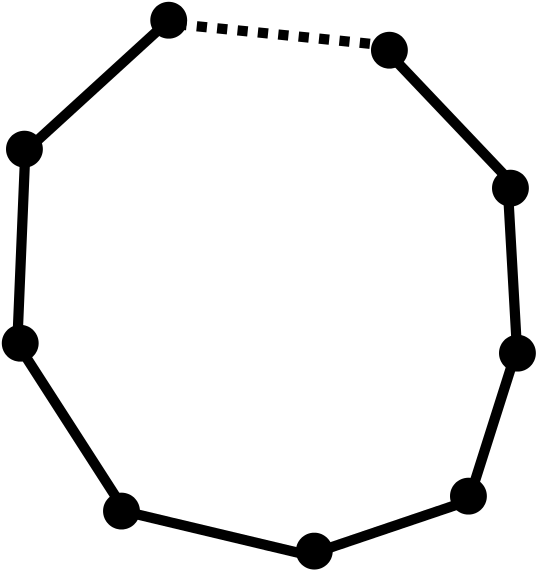
\includegraphics[width=.5\textwidth]{images/cycle.png}
        \caption*{\footnotesize{$G_1$：由$n$个点组成的环}}
     \end{subfigure}
     \hfill
     \begin{subfigure}[T]{0.48\textwidth}
         \centering
         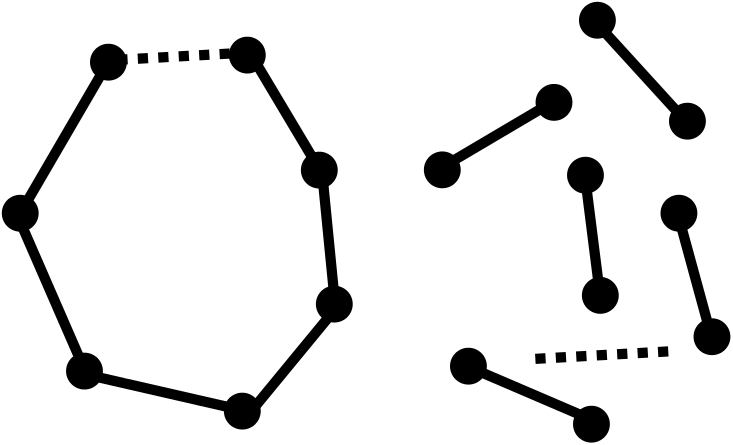
\includegraphics[width=.85\textwidth]{images/far.png}
        \caption*{\footnotesize{$G_2$：一个长为$\frac{n}{2}$的环$+ \frac{n}{4}$条互不相交的边}}
     \end{subfigure}
\end{figure}

为了区分$G_1$和$G_2$，可以采样常数个点（比如采样10个点），然后从采样的这些点出发，做两步广度优先搜索。
如果在搜索的过程中发现了孤立的边，说明是$G_2$，输出No（即不连通）。

\textbf{证明思路：}在$G_2$中，连着孤立边的点有$\frac{n}{4}\cdot 2=\frac{n}{2}$个，占总数的一半，均匀随机地采样10个点，采样的点全都没连到孤立边的概率是$(\frac{1}{2})^{10}$。
只要采样到孤立边对应的点，经过两步广度优先搜索，就一定能判断该图是$G_2$。
因此，以至少$1-\frac{1}{2^{10}}\ge\frac 23$的概率，采样10个点就能区分$G_1$和$G_2$。



如果要精确地判断一个任意的图是否连通，算法至少需要$\Omega(n+m)$次查询，例如，图中只有一个点是孤立的，其余所有点都连通，算法必须找到孤立点，则需要遍历所有的点。
因此，要设计亚线性时间的算法，我们允许算法对图的性质进行近似。



\subsection{检测连通性(度数受限图下的邻接链表模型)}
假设图$G$的最大度数是一个常数，记为$d$。远离性质$P$的形式化定义如下：
\begin{definition}
    如果需要对图$G$修改至少$\varepsilon dn$条边才能使得$G$满足性质$P$（修改边之后最大度数仍然是$d$），就称图$G$是$\varepsilon$-远离性质$P$的。
\end{definition}

例如，在\cref{fig:connectivity}中，左图是连通的，而右图更稀疏，需要添加很多条边才能连通，是\textit{远离}连通性的。

\begin{figure}[!ht]
     \centering
     \begin{subfigure}[T]{0.48\textwidth}
        \centering
        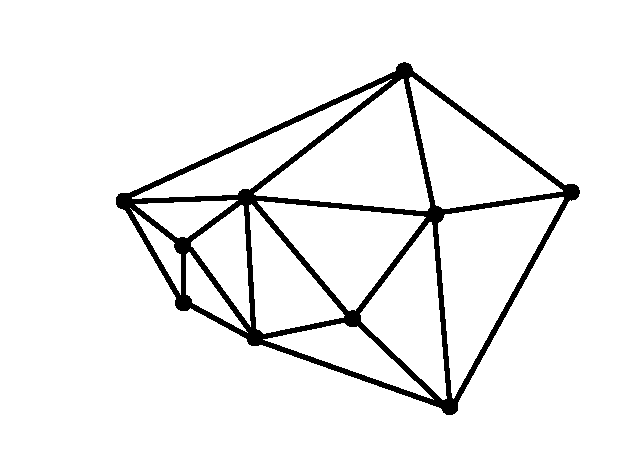
\includegraphics[height=4cm]{images/connected.eps}
	\caption*{连通图}
     \end{subfigure}
     \hfill
     \begin{subfigure}[T]{0.48\textwidth}
         \centering
         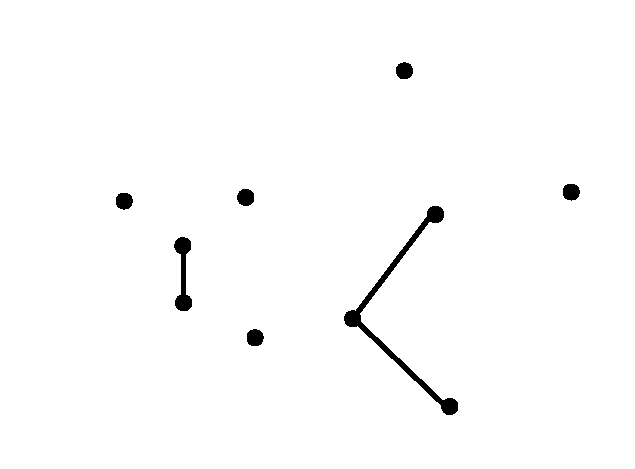
\includegraphics[height=4cm]{images/farconnected.eps}
	\caption*{远离连通性的图}
     \end{subfigure}
     \caption{图的连通性检测}
     \label{fig:connectivity}
\end{figure}

对于远离连通的图，我们观察到：如果一个图是远离连通的，
图中应该有大量较小的连通片（连通片的大小即该连通片包含的点的数量）。
因此我们通过采样一些点，再从这些点出发做广度优先搜索，就能把小的连通片挖掘出来，从而判断图的连通性。
这个观察可以形式化地表现为下面这个断言。
\begin{claim}[\cite{goldreich1997property}]\label{claim:smallCCs}
    如果图$G$是$\varepsilon$-远离连通性，则至少有$\frac{\varepsilon d n}{8}$个连通片的大小是$\le\frac{8}{\varepsilon d}$的。
\end{claim}

\begin{proof}
    记图$G$的连通片数量为$c$。当$G$不连通时，需要添加$c-1$条边才能使其连通（将所有连通片连起来）。
    由于$G$是$\varepsilon$-远离连通性，至少需要修改$\varepsilon dn$条边才能使$G$连通。
    因此，$c-1\ge\varepsilon dn$，即$c\ge\varepsilon dn$。

    记$G$中连通片大小超过$\frac{8}{\varepsilon d}$的数量为$c_1$，
    大小$\le\frac{8}{\varepsilon d}$的连通片的数量为$c_2$，则$c_1+c_2=c$。由于
    \[
    n=\text{$G$中的顶点数}=\sum_{\text{$G$中的连通片$S$}}|S|\ge\sum_{S:|S|>\frac{8}{\varepsilon d}}|S|\ge c_1\cdot\frac{8}{\varepsilon d}
    \]

    所以$c_1\le\frac{\varepsilon dn}{8}$，因此$c_2=c-c_1\ge \varepsilon dn-\frac{\varepsilon dn}{8}\ge\frac{\varepsilon dn}{8}$。
    该断言得证。
\end{proof}

基于以上观察，我们可以设计判断图的连通性的亚线性\textbf{算法}，\textsc{TestingConnectivity}：
\begin{enumerate}
    \item 重复$s=O(\frac{1}{\varepsilon d})$次迭代：
    \begin{enumerate}
        \item[1.1] 均匀随机地采样一个顶点$u$
        \item[1.2] 判断$u$所在的连通片的大小是否较小：
        \begin{enumerate}
            \item[1.2.1] 从$u$出发进行广度优先搜索。如果把$u$所在的连通片都访问完，
            或者已经访问了$t:=\Theta(\frac{1}{\varepsilon d})$个顶点，结束搜索。
            \item[1.2.2] 如果发现了一个大小$<t$的连通片，\textbf{拒绝}图$G$（即认为$G$远离连通性）
        \end{enumerate}
    \end{enumerate}
    \item \textbf{接受}图$G$（即认为$G$是连通的）
\end{enumerate}

\begin{algorithm}[h]
\caption{\textbf{连通性检测算法}}
	\label{alg-connectivity-test}
\begin{enumerate}
    \item \textbf{Input:} 一个整数 $ n \in \mathbb{Z}_{>0} $，$ \epsilon \in (0, 1) $，以及对图 $ G $ 上 $ n $ 个顶点的查询访问。
    \item \textbf{for} $ s := \Theta(1/(d \epsilon)) $ 次 \textbf{do}
    \begin{enumerate}
        \item 从 $ V $ 中随机均匀地抽样一个顶点 $ v $。
        \item 从 $ v $ 开始进行广度优先搜索（BFS），直到到达 $ 2/(d \epsilon) $ 个顶点，或者无法到达新的顶点为止。
        \item \textbf{if} 找到了一个（大小小于 $ n $ 的）连通分量 \textbf{then}
        \begin{enumerate}
            \item 拒绝。
        \end{enumerate}
        \item \textbf{end if}
    \end{enumerate}
    \item \textbf{end for}
    \item 接受。
\end{enumerate}
\end{algorithm}


\begin{theorem}[\cite{goldreich1997property}]
    算法\textsc{TestingConnectivity}能在$O(\frac{1}{\varepsilon^2d})$次查询内，检测图的连通性。
\end{theorem}

\begin{proof}
    \textbf{查询复杂度：}从每个被采样的点出发，广度优先搜索最多访问$\Theta(\frac{1}{\varepsilon d})$个点，
    最多有$\Theta(\frac{1}{\varepsilon d}\cdot d)=\Theta(\frac{1}{\varepsilon})$次查询。
    算法采样了$O(\frac{1}{\varepsilon d})$个点，因此总查询复杂度是$O(\frac{1}{\varepsilon d}\cdot\frac{1}{\varepsilon})=O(\frac{1}{\varepsilon^2 d})$。

    \textbf{正确性：}如果图$G$是连通的，算法\textsc{TestingConnectivity}不会发现大小$<t$的连通片，因此一定会接受$G$。
    如果$G$是$\varepsilon$-远离连通性，令$t=\frac{8}{\varepsilon d}$，则根据\cref{claim:smallCCs}，
    大小$<t$的连通片至少有$\frac{\varepsilon dn}{8}$个，占顶点总数的比例为$\frac{\varepsilon dn}{8}/n=\frac{\varepsilon d}{8}$。
    取$s=2/\frac{\varepsilon d}{8}=\frac{16}{\varepsilon d}$，
    则采样$s$个点均没有落在$<t$的连通片内的概率最多是
    \[
    \left(1-\frac{\varepsilon d}{8}\right)^s<e^{-\frac{\varepsilon d}{8}\cdot s}=e^{-2}<\frac{1}{3}
    \]

    因此，当$G$是$\varepsilon$-远离连通性时，以至少$\frac{2}{3}$的概率，采样的$s$个点中，至少存在一个点所在的连通片大小是$<t$，算法就会拒绝$G$。
\end{proof}

\subsection{检测二部性（稠密图上的邻接矩阵模型）}

在本节中，我们展示二分图性质是可用常数查询测试的。我们的算法同样简单明了：我们从顶点集 $ V $ 中抽样一个大小为常数的顶点集 $ S $，通过查询 $ S $ 中所有顶点对，得到诱导子图 $ G[S] $，然后检查该诱导子图 $ G[S] $ 是否为二分图。详见算法\Cref{alg-bipartite-test}。
\begin{algorithm}[h]
	\caption{\textbf{二部性检测算法}}
	\label{alg-bipartite-test}
	\begin{enumerate}
    \item \textbf{Input:} 一个整数 $ n \in \mathbb{Z}_{>0} $，$ \epsilon \in (0, 1) $，以及对图 $ G = (V, E) $ 上 $ n $ 个顶点的查询访问。
    \item 随机均匀地选择一个顶点集 $ S $，其中 $ |S| = \Theta(\epsilon^{-2} \log \epsilon^{-1}) $。
    \item 查询所有顶点对 $ (u, v) $，其中 $ u, v \in S $。
    \item \textbf{if} $ G[S] $ 是二分图 \textbf{then}
    \item \hspace{1em} 接受。
    \item \textbf{else}
    \item \hspace{1em} 拒绝。
    \item \textbf{end if}
\end{enumerate}
\end{algorithm}

\begin{theorem}
\Cref{alg-bipartite-test}以至少$2/3$的概率成功。
\end{theorem}
\begin{proof}
若 $G$ 是二分图，则其任意导出子图（包括 $G[S]$）也是二分图，因此算法会接受。

现在假设 $G$ 与任意二分图的距离至少为 $\epsilon$（即 $\epsilon$-远）。证明的主要思想如下：  
将采样集 $S$ 划分为两个不交集合 $T$ 与 $U$，其中  
$$
|T| = \frac{4}{\epsilon} \cdot \ln\!\left( \frac{\epsilon}{8/3} \right),
$$
集合 $U$ 由剩余的采样顶点组成。我们首先证明：以高概率，几乎所有顶点都至少有一个邻居在 $T$ 中。暂且假设这一条件成立。

考虑任意一个 $T$ 的二染色 $\chi : T \to \{\text{红}, \text{蓝}\}$。若要将 $\chi$ 扩展为整个图的合法二染色，一个必要条件是：红色顶点的邻居必须是蓝色，蓝色顶点的邻居必须是红色。这样，$T$ 的一个固定染色为 $V \setminus T$ 中的每个顶点施加了一个必要的颜色限制（若某顶点同时邻接红蓝两色顶点，则我们可视作它仅邻接蓝色顶点）。

据此，我们得到一个扩展染色 $\chi'$，它可能合法也可能不合法，但一定满足上述必要条件，且它为 $U$ 中的顶点确定了颜色。由于 $G$ 是 $\epsilon$-远离二分图的，因此在染色 $\chi'$ 下至少有 $\epsilon n^2$ 条单色边。

我们将 $U$ 划分为
$$
\epsilon^2 \cdot \big(|T| + \ln(6)\big)
$$
对（如果有剩余顶点则忽略）。任意一对顶点命中单色边的概率至少为 $\epsilon$，因此所有对都未命中单色边的概率至多为
$$
(1 - \epsilon)^{\epsilon^2 (|T| + \ln 6)} \le \frac{1}{6} \cdot 2^{-|T|}.
$$
因此：
$$
\Pr[\exists\ \text{$T \cup U$ 的合法二染色}] \le
\sum_{\chi \ \text{为}\ T\ \text{的二染色}} \Pr[U\ \text{对}\ \chi' \ \text{无单色边}]
\le 2^{|T|} \cdot \frac{1}{3} \cdot 2^{-|T|} = \frac{1}{3}.
$$

接下来考虑并非每个顶点都有邻居在 $T$ 的情形。定义
$$
\Gamma(T) = T \cup \{ v \in V \setminus T \mid \exists u \in T,\ (u,v) \in E \}.
$$

\begin{claim}
若 $|T| \ge \frac{4}{\epsilon} \ln\!\left( \frac{\epsilon}{8/3} \right)$，则以概率至少 $1 - \frac13$ 有
$$
\sum_{v \notin \Gamma(T)} \deg(v) \le \frac{\epsilon n^2}{2}.
$$
\end{claim}

\begin{proof}
对于度数至少 $\epsilon n/4$ 的顶点 $v$，有
$$
\Pr[v \notin \Gamma(T)] \le (1 - \epsilon/4)^{|T|} \le \frac{\epsilon}{8/3}.
$$
记 $X_v$ 为指示变量，表示事件 $v \notin \Gamma(T)$。则
$$
\mathbb{E}[X_v] \le \frac{\epsilon}{8/3}, \quad
\mathbb{E}\left[ \sum_{v \in V} X_v \right] \le \frac{\epsilon n}{8/3}.
$$
由 Markov 不等式可得
$$
\Pr\left[ \sum_{v \in V} X_v > \frac{\epsilon n}{4} \right] < \frac13.
$$
由于任意顶点度数 $\le n$，可得结论成立。
\end{proof}


假设 $T$ 是好的（即满足上述结论），并取 $T$ 的一个合法二染色 $\chi$。定义扩展染色 $\chi'$ 如下：
$$
\chi'(v) =
\begin{cases}
\chi(v), & v \in T, \\
1, & \exists u \in T, (u,v) \in E, \chi(u) = 2, \\
2, & \text{否则}.
\end{cases}
$$

\begin{claim}
若 $G$ 是 $\epsilon$-远离二分图，且 $\sum_{v \notin \Gamma(T)} \deg(v) \le \frac{\epsilon n^2}{2}$，则在 $\Gamma(T)$ 中由 $\chi'$ 诱导的单色边数超过 $\frac{\epsilon n^2}{2}$。
\end{claim}

\begin{proof}
由于 $G$ 是 $\epsilon$-远离二分图，任何染色 $\chi'$ 都至少有 $\epsilon n^2$ 条单色边。其中至多 $\frac{\epsilon n^2}{2}$ 条与 $V \setminus \Gamma(T)$ 相邻，因此 $\Gamma(T)$ 中的单色边数超过 $\frac{\epsilon n^2}{2}$。
\end{proof}

最后，将 $U$ 划分为
$$
\frac{2}{\epsilon} \cdot \left(|T| + \ln 6\right)
$$
对。由上述引理，每对顶点命中单色边的概率至少为 $\epsilon/2$，因此无对命中单色边的概率至多
$$
(1 - \epsilon/2)^{\epsilon^2 (|T| + \ln 6)} \le \frac{1}{6} \cdot 2^{-|T|}.
$$
综合各项概率估计可知，算法接受的概率至多 $1/3$，因此拒绝的概率至少为 $2/3$。
\end{proof}

\section{参数近似}
\textbf{目标：}通过查询模型对图进行访问，要求在尽可能少的查询次数下，比较好地近似图中的一些参数。例如：最小生成树的权重的值，边的数量，最大匹配的大小，给定子图的数量等。

\subsection{估算最小生成树的权重}
在本小节中，我们研究近似最小生成树的权重。即：在图$G=(V,E)$中找到一棵树$T\subseteq E$，
使得树的权重$w(T)=\sum_{(u,v)\in T}w(u,v)$最小。最小的权重对应的树记为$T^*$，其权重记为$w(G)=w(T^*)$。
注意到，如果精确地计算最小生成树或者其权重，需要线性的时间，但我们可以在亚线性时间内对其权重进行近似。

\subsubsection{最小生成树权重的公式}

\begin{definition}
    记$G^{(\ell)}$表示$G$的子图，$G^{(\ell)}$的顶点集合与$G$相同，
    边集包含$G$中所有权重$\le\ell$的边。记$G^{(\ell)}$中连通片的数量为$c^{(\ell)}$。
\end{definition}

基于上述定义，我们有以下观察：

\begin{claim}\label{claim:MST-CC}
    记$n=|V|$为图$G$的顶点数，$W$表示$G$的最大权重。则$G$中最小生成树的权重满足：$w(G)=n-W+\sum_{i=1}^{W-1}c^{(i)}$。
\end{claim}
\begin{proof}
    记MST中权重为$i$的边的数量为$\alpha_i$，根据Kruskal算法，不同的MST中，$\alpha_i$的值是一样的。
    观察到：
    \begin{itemize}
        \item $\sum_{i=1}^W \alpha_i=n-1$，因为最小生成树上一共有$n-1$条边
        \item 对于任意的$\ell\in[W]$，有$\sum_{i>l}\alpha_i=c^{(\ell)}-1$，因为要想把$G^{(\ell)}$中的所有连通片连起来，
        需要用到$c^{(\ell)-1}$条边，而这些边的权重都$>\ell$，且使用最小生成树上的边就足够把这些连通片连起来了（因为最小生成树是连通的）
        \item $c^{(0)}=n$，因为已经假设图$G$的边权属于$\{1,\dots,W\}$，没有一条边的权重是0，
        因此$G^{(0)}$中没有一条边，每个顶点都是孤立点
    \end{itemize}

    因此，最小生成树的权重可以写成：
    \begin{align*}
        w(G)=&\sum_{i=1}^W i\cdot\alpha_i\\
        &=\sum_{j=1}^W(\sum_{i=j}^W \alpha_i)\\
        &=\sum_{j=1}^W (c^{(j-1)}-1) \tag{利用$\sum_{i>\ell}\alpha_i=c^{(\ell)}-1$}\\
        &=n-W+\sum_{j=1}^{W-1}c^{(j)}
    \end{align*}
\end{proof}

\subsubsection{估算连通片的数量}
有了\cref{claim:MST-CC}，我们就只需要估算$c^{(\ell)}$，即每个子图$G^{(\ell)}$的连通片的数量。

对顶点$u$，记$n(u)$表示$u$所在的连通片中顶点的数量。
对任意连通片$A$，观察到：$\sum_{u\in A}\frac{1}{n(u)}=\sum_{u\in A}\frac{1}{|A|}=1$。
进一步，记图$G$的全体连通片的集合为$\cC$，则有：
$\sum_{v\in V}\frac{1}{n(v)}=\sum_{A\in\cC}\sum_{u\in A}\frac{1}{n(u)}=\sum_{A\in\cC}1=|\cC|$，即图中连通片的数量。

因此，如果对每个顶点$v$，$n(v)$的值是已知的，
我们只需要进行简单的操作即可估算连通片的数量：
\begin{enumerate}
    \item 将求和$sum$初始化为0
    \item 重复$s$次迭代：
    \begin{enumerate}
        \item[2.1] 均匀随机地采样一个点$v\in V$
        \item[2.2] 计算$sum\leftarrow sum+\frac{1}{n(v)}$
    \end{enumerate}
    \item 输出$\tilde{c}=n\cdot\frac{sum}{s}$
\end{enumerate}

当然，实际情况中，$n(v)$是未知的，因此我们考虑估算$n(v)$的值。
参考算法\textsc{TestConnectivity}，我们得到一个估算连通片数量的\textbf{算法}$\cA$：
\begin{enumerate}
    \item 将求和$sum$初始化为0
    \item 重复$s=O(1/\varepsilon^3)$次迭代：
    \begin{enumerate}
        \item[2.1] 均匀随机地采样一个点$v\in V$
        \item[2.2] 从$v$出发做广度优先搜索，如果在遍历完整个连通片之前访问了超过
        $\frac{2}{\varepsilon}$个顶点，令$\tilde{n}(v)=\frac{2}{\varepsilon}$；
        
        否则，如果遍历完整个连通片时访问的点数$\le\frac{2}{\varepsilon}$，
        令$\tilde{n}(v)=n(v)$，即访问的点数
        \item[2.3] 计算$sum\leftarrow sum+\frac{1}{\tilde{n}(v)}$
    \end{enumerate}
    \item 输出$\tilde{c}=n\cdot\frac{sum}{s}$
\end{enumerate}

\begin{lemma}\label{lem:appncc}
    对于图$G$，记其连通片的数量为$c$。上述算法$\cA$
    输出的估计值$\tilde{c}$，以至少$\frac{2}{3}$的概率满足$|\tilde{c}-c|\le\varepsilon n$。
    算法$\cA$的运行时间为$O(\frac{d}{\varepsilon^4})$
\end{lemma}
\begin{proof}
    \textbf{运行时间：}对于每个采样的顶点，从它出发探索的点数最多为$\frac{2}{\varepsilon}$，
    由于顶点度数最大是$d$，因此广度优先搜索的时间是$O(\frac{d}{\varepsilon})$。
    因为采样了$O(1/\varepsilon^3)$个顶点，所以总的运行时间为$O(\frac{d}{\varepsilon}/\varepsilon^3)=O(\frac{d}{\varepsilon^4})$。

    \textbf{正确性：}记
    $\hat{n}(u)=\min\{n_u,\frac{2}{\varepsilon}\}$，
    $\hat{c}:=\sum_{u\in V}\frac{1}{\hat{n}(u)}$。
    则：对于任意的顶点$u$，$|\frac{1}{\hat{n}(u)}-\frac{1}{n(u)}|\le\frac{\varepsilon}{2}$。
    因为当$n_u<\frac{2}{\varepsilon}$时，$\hat{n}(u)=n(u)$，此时$\frac{1}{\hat{n}(u)}-\frac{1}{{n}(u)}=0$；
    而当$n_u\ge\frac{2}{\varepsilon}$时，$0<\frac{1}{{n}(u)}\le\frac{1}{\hat{n}(u)}=\frac{\varepsilon}{2}$，
    所以$\frac{1}{\hat{n}(u)}-\frac{1}{{n}(u)}\le\frac{\varepsilon}{2}$。

    因此，有$|\hat{c}-c|=|\sum_{u\in V}\frac{1}{\hat{n}(u)}-\frac{1}{n(u)}|\le\sum_{u\in V}|\frac{1}{\hat{n}(u)}-\frac{1}{{n}(u)}|
    \le\sum_{u\in V}\frac{\varepsilon}{2}=\frac{\varepsilon n}{2}$。

    此外，由于$1\le\hat{n}(u)\le\frac{2}{\varepsilon}$，对任意的$u$，有$\frac{\varepsilon}{2}\le\frac{1}{\hat{n}(u)}\le1$，
    因此$\frac{\varepsilon n}{2}\le\hat{c}\le n$。

    对于第$i$个采样的点，记估计值$\frac{1}{\tilde{n}(u)}$为$X_i\in[0,1]$，计算它的期望：
    $\E[X_i]=\frac{1}{n}\sum_{u\in V}\frac{1}{\hat{n}(u)}=\frac{\hat{c}}{n}$。

    由于$\frac{s}{n}\tilde{c}=\sum_{i=1}^s X_i$，其期望为
    $\E[\sum_{i=1}^s X_i]=s\cdot \E[X_1]=\frac{s\hat{c}}{n}$。
    记$X=\sum_{i=1}^s X_i$，
    根据Chernoff-Hoeffding Bound（见笔记\textit{Notes Lec1 概率论回顾}），有
    \begin{align*}
        \Pr[|\tilde{c}-\hat{c}|\ge\frac{\varepsilon \hat{c}}{2}]&=\Pr[|\frac{s}{n}\tilde{c}-\frac{s}{n}\hat{c}|\ge\frac{\varepsilon}{2}\cdot\frac{s\hat{c}}{n}]\\
        &=\Pr[|X-\E[X]|\ge\frac{\varepsilon}{2}\E[X]]\\
        &\le 2\exp(-\frac{\E[X]\cdot\varepsilon^2/2^2}{3})\\
        &=2\exp(-\frac{s\hat{c}\varepsilon^2}{12n}) \tag{代入$\E[X]$}\\
        &\le2\exp(-O(\frac{1}{\varepsilon^3})\cdot\frac{\varepsilon n}{2}\cdot\frac{\varepsilon^2}{12n}) \tag{由于$s=O(1/\varepsilon^3)$且$\hat{c}\ge\frac{\varepsilon n}{2}$}\\
        &\le\frac{1}{3} \tag{通过选取$s=b/\varepsilon^3$中的常数$b$可以实现}
    \end{align*}

    因此，以至少$\frac{2}{3}$的概率，$|\tilde{c}-c|\le|\tilde{c}-\hat{c}|+|\hat{c}-c|\le\frac{\varepsilon\hat{c}}{2}+\frac{\varepsilon n}{2}\le \varepsilon n$。
\end{proof}

\subsubsection{估算最小生成树权重的算法}

根据算法$\cA$，设计估算最小生成树权重的\textbf{算法}$\cB$：
令$\varepsilon'=\frac{\varepsilon}{W}$，再使用median trick增强算法的成功概率，对每个子图$G^{(i)}$调用算法$\cA$得到$\tilde{c}^{(i)}$。
输出$\tilde{w}(G)=n-W+\sum_{i=1}^{W-1}\tilde{c}^{(i)}$。

\begin{theorem}\label{thm:appmst}
    图$G$有$n$个顶点，假设图中每条边的权重都是区间$[1,W]$内的整数，
    则存在一个算法输出估计值$\tilde{w}(G)$，以至少$\frac{2}{3}$的概率满足
    \[
    (1-\varepsilon)\cdot w(G)\le \tilde{w}(G)\le(1+\varepsilon)\cdot w(G)
    \]

    该算法的运行时间为$\tilde{O}(d\cdot W^5/\varepsilon^5)$。
\end{theorem}
\begin{proof}
    根据\cref{lem:appncc}，算法$\cB$得到的任意一个$\tilde{c}^{(i)}$以至少$1-\frac{1}{\poly(W)}$的概率满足$|\tilde{c}^{(i)}-c^{(i)}|\le\frac{\varepsilon n}{W}$。
    因此，利用union bound，对\textit{所有的}$i\in[W]$，该不等式都满足的概率是$1-\frac{1}{\poly(W)}$。下面假设这个事件发生。

    得到$\tilde{w}(G)$的运行时间为
    $W\cdot\tilde{O}(\frac{d}{(\varepsilon/W)^4})=\tilde{O}(\frac{W^5d}{\varepsilon^4})$。
    其理论保证为
    \begin{align*}
        |w(G)-\tilde{w}(G)|&=\left|\left(n-W+\sum_{i=1}^{W-1}{c}^{(i)}\right)-\left(n-W+\sum_{i=1}^{W-1}\tilde{c}^{(i)}\right)\right| \tag{根据\cref{claim:MST-CC}}\\
        &\le\sum_{i=1}^{W-1}|\tilde{c}^{(i)}-c^{(i)}| \\
        &\le(W-1)\frac{\varepsilon n}{W} \tag{根据$\tilde{c}^{(i)}$的理论保证}\\
        &<\varepsilon n\\
        &\le 2\varepsilon\cdot w(G) \tag{由于$c^{(i)}\ge 1$，$w(G)\ge n-W+W-1\ge\frac{n}{2}$，当$n\ge2$时}
    \end{align*}
\end{proof}

\subsection{估算图的平均度数}
\problem 对于一个\textbf{连通}的图$G=(V,E)$，其顶点集合为$V=[n]:=\{1,\dots,n\}$。
图中一个点$v$的度数，是和它相连的边数，记为$\deg(v)$。
对图的访问可以是仅允许查询任意顶点的度数，也可以包含查询顶点的邻居。
目标是在亚线性时间内估算图的平均度数，即估算$d_{\avg}=\frac{1}{n}\sum_{v\in V}\deg(v)$。

\subsubsection{查询图的度数}
如果只允许查询图中顶点的度数（不允许查询顶点的邻边），这个问题是很难的。

考虑一个星状图$G_1$，即一个中心点连着其他所有顶点，除此之外图中没有别的边。
在这个图里，只有一个顶点的度数是$n-1$，其余顶点的度数都是$1$，
平均度数为$d_{\avg}=\frac{(n-1)\cdot1+1\cdot(n-1)}{n}\approx2$。
要做到2-近似，就一定要访问中心点，否则得到的平均度数是1（2-近似指，算法输出的估算值$R$满足$d_{\avg}\le R\le2d_{\avg}$）。

更进一步，考虑图$G_2$，其中有100个顶点的度数是$n-1$，其余顶点的度数都是1，
平均度数为$d_{\avg}=\frac{(n-100)\cdot1+100\cdot(n-1)}{n}\approx 101$，
那要想做到比100更好的近似比，就需要找到这100个特殊的顶点，需要$\Omega(n)$次查询。
100也可以换成别的常数，这样看来似乎在亚线性时间下，常数近似都做不到。
但$G_2$这样的图是不存在的，因为顶点的度数需要符合图数据结构的规则。

事实上，存在一个亚线性时间的\textbf{算法}\textsc{AvgDeg-V1}，可以做到$(2+\varepsilon)$-近似：
\begin{enumerate}
    \item 调用子程序\textsc{AvgNibble} $t:=\frac{8}{\varepsilon}$次，
    得到估算值$d_{S_1},\dots,d_{S_t}$
    \item 输出这些估算值中的最小值，即输出$R:=\min_{i=1}^t d_{S_i}$
\end{enumerate}

子程序\textsc{AvgNibble}的描述如下：
\begin{enumerate}
    \item 给定某个足够大的常数$\beta>0$，
    采样$s=\frac{\beta\sqrt{n}}{\varepsilon^3}$个点，采样的顶点集合记为$S$
    \item 输出采样的点的平均度数，即输出$d_S:=\frac{\sum_{i\in S}\deg(i)}{s}$
\end{enumerate}


\begin{theorem}\label{thm:avgdeg-v1}
    令$0<\varepsilon<\frac{1}{3}$为一个常数。
    假设算法只允许查询顶点的度数，则\textsc{AvgDeg-V1}算法输出的$R$
    以至少$\frac{3}{4}$的概率满足
    $(\frac{1}{2}-\varepsilon)d_{\avg}\le R\le(1+\varepsilon)d_{\avg}$，
    且运行时间为$O(\sqrt{n}/\varepsilon^4)$。
\end{theorem}

注意到，根据\cref{thm:avgdeg-v1}，有$d_{\avg}\le\frac{1}{1/2-\varepsilon}R\le\frac{1+\varepsilon}{1/2-\varepsilon}d_\avg$，
其中由于$\frac{1}{1-2\varepsilon}\le 1+3\varepsilon$，有
$\frac{1+\varepsilon}{1/2-\varepsilon}\le(2+2\varepsilon)(1+3\varepsilon)=2+O(\varepsilon)$。
令$R'=\frac{1}{1/2-\varepsilon}R$，则$R'$的近似比为$2+\varepsilon$。

为了证明\cref{thm:avgdeg-v1}，需要先证两个引理。

\begin{lemma}\label{lem:nibble-A}
    以至少$1-\frac{1}{1+\varepsilon}\ge\frac{\varepsilon}{2}$的概率，
    算法\textsc{AvgNibble}输出的$d_S$满足$d_S\le(1+\varepsilon)\cdot d_\avg$。
\end{lemma}
\begin{proof}
    令$X_i$表示第$i$个采样的点的度数，由于是均匀随机采样，
    有$\Pr[\text{第$i$个被采样到的顶点为}j]=\Pr[X_i=\deg(j)]=\frac{1}{n}$，。
    因此，
    \[
    \E[X_i]=\sum_{j=1}^n\deg(j)\Pr[X_i=\deg(j)]=\sum_{j=1}^n\deg(j)\cdot\frac{1}{n}=d_\avg
    \]

    由于$d_S=\frac{\sum_{i\in S}\deg(i)}{s}$，
    有$\E[d_S]=\E[\frac{1}{s}\sum_{i=1}^sX_i]=d_\avg$。
    根据Markov不等式，
    \[
    \Pr[d_S>(1+\varepsilon)d_\avg]\le\frac{\E[d_S]}{(1+\varepsilon)d_\avg}=\frac{1}{1+\varepsilon}
    \]
\end{proof}

\begin{lemma}\label{lem:nibble-B}
    以至少$1-\frac{\varepsilon}{64}$的概率，
    算法\textsc{AvgNibble}输出的$d_S$满足$d_S\ge(\frac{1}{2}-\varepsilon)\cdot d_\avg$。
\end{lemma}
\begin{proof}
    对于图$G=(V,E)$，定义$H$为度数最高的$\sqrt{\frac{\varepsilon}{2}n}$个顶点的集合，
    $L=V\setminus H$。

    首先，由于$\sum_{i=1}^n\deg(i)=2|E|$，则$L$和$H$之间的边满足
    $|E(L,H)|\le|E|\le\frac{1}{2}\sum_{i=1}^n\deg(i)$。

    其次，由于$H$中只有$\sqrt{\frac{\varepsilon}{2}n}$个顶点，所以
    $2|E(H)|\le|V(H)|^2=\frac{\varepsilon n}{2}$。

    此外，由于图$G$是连通的，至少有$n-1$条边，所以$\sum_{i=1}^n\deg(i)=2|E|\ge2(n-1)$。
    因此，有
    \[
    2|E(H)|\le\frac{\varepsilon}{2}n\le\frac{\varepsilon}{2}2(n-1)
    \le\frac{\varepsilon}{2}\cdot\sum_{i=1}^n\deg(i)
    \]

    $L$中的点的度数之和满足$\sum_{i\in L}\deg(i)=\sum_{i=1}^n\deg(i)-|E(L,H)|-2|E(H)|$。
    记$L$中顶点的平均度数为$d_L$，则有
    $d_L=\frac{\sum_{i\in L}\deg(i)}{|L|}\ge\frac{(\frac{1}{2}-\frac{1}{2}\varepsilon)\sum_{i=1}^n\deg(i)}{n}=(\frac{1}{2}-\frac{1}{2}\varepsilon)d_\avg$。

    由于这个引理在求$d_S$的下界，我们可以假设所有采样到的顶点都来自$L$。
    定义$D_H$为$H$中最小的度数，$X_i$为第$i$个被采样到的顶点的度数。
    则$\E[X_i]\ge d_L=\frac{\sum_{i\in L}\deg(i)}{|L|}\ge(\frac{1}{2}-\frac{1}{2}\varepsilon)d_\avg$。
    
    由于$d_S=\frac{\sum_{i=1}^sX_i}{s}$，则$E[d_S]=\frac{1}{s}\E[\sum_{i=1}^sX_i]\ge(\frac{1}{2}-\frac{1}{2}\varepsilon)d_\avg$。
    等价地，有$(\frac{1}{2}-\varepsilon)d_\avg\le\frac{\frac{1}{2}-\varepsilon}{\frac{1}{2}-\frac{1}{2}\varepsilon}\E[d_S]\le(1-\varepsilon)\E[d_S]$。

    另一方面，对于平均度数，有$d_\avg=\frac{1}{n}\sum_{i=1}^n\deg(i)\ge\frac{\sum_{i\in H}\deg(i)}{n}\ge\frac{D_H\cdot|H|}{n}$，
    因此$\E[d_S]\ge\frac{(\frac{1}{2}-\frac{1}{2}\varepsilon)D_H\cdot|H|}{n}$，
    且$\E[\sum_{i=1}^sX_i]\ge\frac{(\frac{1}{2}-\frac{1}{2}\varepsilon)D_H\cdot|H|\cdot s}{n}$。
    根据Chernoff Bound，有
    \begin{align*}
        \Pr[d_S\le(\frac{1}{2}-\varepsilon)d_\avg]&\le\Pr[d_S\le(1-\varepsilon)\E[d_S]]\\
        &=\Pr[\frac{1}{s}\sum_{i=1}^sX_i\le(1-\varepsilon)\frac{1}{s}\E[\sum_{i=1}^sX_i]]\\
        &=\Pr[\frac{1}{D_H}\sum_{i=1}^sX_i\le(1-\varepsilon)\frac{1}{D_H}\E[\sum_{i=1}^sX_i]]\\
        &\le2\exp(\frac{-\E[\sum_{i=1}^sX_i]\cdot\varepsilon^2}{3\cdot D_H}) \tag{假设采样的点都来自$L$，有$0\le\frac{X_i}{D_H}\le1$}\\
        &\le2\exp(\frac{-s\cdot|H|}{n}\cdot(\frac{1}{2}-\frac{1}{2}\varepsilon)\cdot\frac{\varepsilon^2}{3})\\
        &\le2\exp(\frac{-s\cdot \varepsilon^{2.5}}{100\sqrt{n}})
    \end{align*}

    因此，令$s=\frac{200\sqrt{n}}{\varepsilon^3}$，即有
    $\Pr[d_S\le(\frac{1}{2}-\varepsilon)d_\avg]\le\frac{\varepsilon}{64}$。
\end{proof}

有了\cref{lem:nibble-A}和\cref{lem:nibble-B}，我们就能证得\cref{thm:avgdeg-v1}。

\begin{proof}[\cref{thm:avgdeg-v1}的证明]
    首先，根据\cref{lem:nibble-B}，以及$(1-\frac{1}{x+1})^x\ge\frac{1}{e}$，有：
    \[
    \Pr[R\ge(\frac{1}{2}-\varepsilon)]=\Pr[\forall i\in[t],d_{S_i}\ge(\frac12-\varepsilon)d_\avg]
    \ge(1-\frac{\varepsilon}{64})^{\frac{8}{\varepsilon}}>\frac{7}{8}
    \]

    其次，根据\cref{lem:nibble-A}，以及$(1-\frac{1}{x})^x\le\frac{1}{e}$，有：
    \begin{align*}
        \Pr[R\le(1+\varepsilon)d_\avg]&=\Pr[\exists i\in[t], d_{S_i}\le(1+\varepsilon)d_\avg]\\
        &=1-\Pr[\forall i\in[t], d_{S_i}>(1+\varepsilon)d_\avg]\\
        &>1-(1-\frac{\varepsilon}{2})^t\\
        &>1-\frac{1}{16}
        \end{align*}
\end{proof}


\subsubsection{查询图的度数和边}
如果算法同时可以访问顶点的度数和邻边，估算平均度数就会容易很多。
在之前的$G_1$的例子中，只能访问顶点度数的算法必须要发现度数为$n-1$的顶点，
才能实现2-近似。但如果算法能访问顶点的邻边，就能很容易地发现度数较高的顶点。

首先先假设一个更简单的情况：假设图$G$是一个几乎正则的图，图中顶点的度数相差不大，
每个顶点的度数都属于区间$[d,10d]$，没有奇异点（即少数点的度数特别大，达到$O(n)$的级别）。
这样的话，算法可以采样一些顶点，计算它们的平均度数。\textbf{算法}描述如下：

\begin{enumerate}
    \item 令$k=\frac{50}{\varepsilon^2}\cdot\ln(\frac{2}{\delta})$，
    \item 对于$i=1,\dots,k$：
    \begin{enumerate}
        \item[2.1] 均匀随机地采样一个顶点，记为$v_i$
        \item[2.2] 令$X_i=\deg(v_i)$
    \end{enumerate}
    \item 输出$\tilde{d}=\frac{1}{k}\sum_{i=1}^kX_i$
\end{enumerate}

\begin{claim}
    上述算法输出的估算值$\tilde{d}$满足$\E[\tilde{d}]=d_\avg$。
\end{claim}

\begin{claim}
    上述算法输出的估算值$\tilde{d}$满足$\Pr[|\tilde{d}-d_\avg|\le\varepsilon d_\avg]\ge1-\delta$，
    且运行时间为$O(\frac{1}{\varepsilon^2}\log\frac{1}{\delta})$。
\end{claim}

在几乎正则的图里，顶点度数的方差很小，因此采样法很有效；
但在一般的图里，有些顶点度数很高，使得方差很大。
如果仍然用最简单的采样法来估计，需要的运行时间是$O(\frac{n}{\varepsilon^2}\cdot\log\frac{1}{\delta})$。

\idea 我们可以考虑减小度数高的顶点带来的方差。由于图的边数是有限的（$|E|=m$），度数很高的顶点不会太多，
我们可以通过引入$\deg^+(v)$，把每条边分配给度数较低的点，从而减小高度数顶点的影响。

具体来说，先定义一个偏序关系$\prec$：如果$\deg(u)<\deg(v)$，或者$\deg(u)=\deg(v)$且$\ID(u)<\ID(v)$，
则称$u\prec v$。
其中，$\ID(v)$表示顶点$v$在集合$V$中的字典序，是输入给定的顺序。
接着，定义$\deg^+(u):=\#\{v\in N(u)|u\prec v\}$，即$u$的邻居中满足$u\prec v$的顶点数。
那么：$\sum_{v\in V}\deg^+(v)=m=\frac{n}{2}\cdot d_\avg$。

尽管一般图中的$\deg(v)$的确会非常大，从而带来很大的方差；
但我们将证明，$\deg^+(v)$对每个顶点$v$来说都是有界的，因此方差更小，
估算$\deg^+(v)$能有更好的理论保证。

\begin{definition}
    定义$H\subset V$是在偏序关系$\prec$下前$\sqrt{2m}$大的顶点集合。
    定义$L:=V\setminus H$。
\end{definition}

\begin{claim}\label{claim:LH-bound}
    对任意顶点$v\in H$，有$\deg^+(v)\le\sqrt{2m}$。

    对任意顶点$v\in L$，有$\deg(v)\le\sqrt{2m}$。
\end{claim}
\begin{proof}
    对于任意$H$中的顶点$v$，$\deg^+(v)$只包含在偏序关系$\prec$下比$v$大的顶点，
    一定也属于$H$，所以$\deg^+(v)\le|H|=\sqrt{2m}$。

    另一方面，对于任意$L$中的顶点$v$，假设$\deg(v)>\sqrt{2m}$，
    那么满足$\deg(u)\ge\deg(v)>\sqrt{2m}$的点$u$一定落在$H$里，
    数量至少是$|H|=\sqrt{2m}$个。则图中的边数
    \[
    m=\frac{1}{2}\sum_{i=1}^n\deg(i)
    \ge\frac{1}{2}\sum_{u:\deg(u)>\deg(v)}\deg(u)
    >\frac{1}{2}\sqrt{2m}\cdot\sqrt{2m} =m
    \]

    出现了矛盾，假设不成立。因此，对任意$v\in L$，有$\deg(v)\le\sqrt{2m}$。
\end{proof}

下面描述\textbf{算法}\textsc{AvgDeg-V2}：
\begin{enumerate}
    \item 令$k=\frac{16}{\varepsilon^2}\cdot\sqrt{n}$
    \item 对于$i=1,\dots,k$：
    \begin{enumerate}
        \item[2.1] 从集合$V$中均匀随机地采样一个点，记为$v_i$
        \item[2.2] 从$v_i$的邻居集合$N(v_i)$中均匀随机地采样一个点，记为$u_i$
        \item[2.3] 如果$v_i\prec u_i$，令$X_i=2\cdot\deg(v_i)$；
        否则，令$X_i=0$
    \end{enumerate}
    \item 输出$R:=\frac{1}{k}\sum_{i=1}^kX_i$
\end{enumerate}

下面这个定理描述了算法\textsc{AvgDeg-V2}的理论保证。

\begin{theorem}
    令$0<\varepsilon<\frac{1}{3}$为一个常数。如果算法能访问顶点的度数和邻边，
    那么算法\textsc{AvgDeg-V2}输出的估算值$R$以至少$\frac{3}{4}$的概率满足
    $(1-\varepsilon)d_\avg\le R\le(1+\varepsilon)d_\avg$，
    且算法的运行时间为$O(\sqrt{n}/\varepsilon^2)$。
\end{theorem}

\begin{proof}
    
\textbf{证明思路：}令$X=\sum_{i=1}^kX_i$，先证明$\E[X]=d_\avg$（是无差估计），且方差很小。
接着用Chebyshev不等式证明估算值$R:=\frac{1}{k}X$的误差很小。

\textbf{证均值：$\E[X_1]=d_\avg$.} 由于是均匀随机采样，每个$X_i$之间是独立的，均值和方差相同，分析$X_1$即可。
\begin{align*}
   \E[X_1]&=\sum_{v\in V}\frac{1}{n}\E[X_1|v\text{被采样}]\\
   &=\sum_{v\in V}\frac{1}{n}\sum_{u\in N(v)}\frac{1}{\deg(v)}\E[X_1|v,u\text{被采样}]\\
   &=\sum_{v\in V}\frac{1}{n}\left(\sum_{u\in N^+(v)}\frac{1}{\deg(v)}\cdot2\deg(v)+ \sum_{u\notin N^+(v)}\frac{1}{\deg(v)}\cdot0\right) \tag{其中，$N^+(v)=\{u\in N(v)|v\prec u\}$}\\
   &= \sum_{v\in V}\frac{2\deg^+(v)}{n}\\
   &= \frac{2m}{n} \tag{根据$\sum_{v\in V}\deg^+(v)=m$}\\
   &= d_\avg
\end{align*}

\textbf{证方差：$\Var[X_1]\le 4\sqrt{2m}\cdot d_\avg$.}
\begin{align*}
    \Var[X_1]&\le\E[X_1^2]\\
    &=\sum_{v\in V}\frac{1}{n}\sum_{u\in N(v)}\frac{1}{\deg(v)}\E[X_1^2|v,u\text{被采样}]\\
    &=\sum_{v\in V}\frac{1}{n}\sum_{u\in N^+(v)}\frac{1}{\deg(v)}(2\deg(v))^2\\
    &=\sum_{v\in V}\frac{4\deg(v)\cdot\deg^+(v)}{n}\\
    &=\frac{4}{n}\left(\sum_{v\in H}\deg(v)\cdot\deg^+(v)+\sum_{v\in L}\deg(v)\cdot\deg^+(v)\right) \tag{因为$V=H\cup L$}\\
    &\le\frac{4}{n}\left(\sum_{v\in H}\deg(v)\cdot\sqrt{2m}+\sum_{v\in L}\sqrt{2m}\cdot\deg(v)\right) \tag{根据\cref{claim:LH-bound}，且$\deg^+(v)\le\deg(v)$}\\
    &\le 4\sqrt{2m}\cdot d_\avg \tag{由于$\frac{\sum_{v\in H}\deg(v)+\sum_{v\in L}\deg(v)}{n}=\frac{\sum_{v\in V}\deg(v)}{n}=d_\avg$}
\end{align*}

由于$R=\frac{1}{k}\sum_{i=1}^kX_i$，有
$\Var[R]=\frac{1}{k}\Var[X_1]\le\frac{4\sqrt{2m}\cdot d_\avg}{\frac{16}{\varepsilon^2}\sqrt{n}}=\frac{\varepsilon^2\sqrt{d_\avg}\cdot d_\avg}{4}$。

\textbf{Chebyshev不等式：}
\[
\Pr[|R-d_\avg|\ge\varepsilon\cdot d_{\avg}]\le\frac{\Var[R]}{\varepsilon^2d_\avg^2}
\le\frac{\varepsilon^2\sqrt{d_\avg}\cdot d_\avg}{4\varepsilon^2\cdot d_\avg^2}
\le\frac{1}{4}
\]

因此，$\Pr[|R-d_\avg|\le\varepsilon\cdot d_\avg]\ge\frac{3}{4}$。

\textbf{运行时间：}对每一轮迭代，采样顶点$v_i$和$u_i$只需要$O(1)$的时间，因此总的运行时间为$O(k)=O(\frac{\sqrt{n}}{\varepsilon^2})$。
\end{proof}

% \printbibliography[heading=subbibliography, title={本章参考文献}]
% \addcontentsline{toc}{section}{参考文献}
% \end{refsection}

% \begin{refsection}
% % ---- Macros migrated from original lecture preamble ----
\providecommand\numberthis{\addtocounter{equation}{1}\tag{\theequation}}

\providecommand{\R}{\mathbb{R}}
\providecommand{\Tr}{\mathrm{Tr}}
\providecommand{\sgn}{\mathrm{sgn}}
\providecommand{\NA}{\mathcal{A}(G)}
\providecommand{\NL}{\mathcal{L}(G)}
\providecommand{\vol}{\mathrm{vol}}
\providecommand{\qf}[2]{{#1}^{\top}{#2}{#1}}
\providecommand{\argmin}{\mathrm{argmin}}

\providecommand*\circled[1]{\tikz[baseline=(char.base)]{
            \node[shape=circle,draw,inner sep=2pt] (char) {#1};}}

\lecture{14}{May 27, 2025}{彭攀}{徐怡，徐航宇，谢凯洋}{谱图论基础：Basics of Spectral Graph Theory}
谱图论通过研究与图相关的矩阵的代数信息（如特征值，特征向量等）来揭示图的组合信息（如两点之间是否连边，是否有最短路径等）。
很多组合优化的经典算法的运行时间都是输入规模的多项式，而使用谱图论的知识，可以得到更高效的算法。下面是几个谱图论的应用场景。

\paragraph{图分割与聚类}
谱图论通过分析拉普拉斯矩阵的特征系统，为图分割和聚类问题提供了强有力的数学工具。与传统基于局部优化的方法相比，谱方法能够捕捉图的全局结构特征，在保证分割质量的同时维持子图平衡性。这种方法在图像分割、社交网络分析和数据聚类等领域展现出显著优势，特别是对于复杂网络结构的识别具有独特价值。

\paragraph{网页排名算法}
基于随机游走理论和马尔可夫链分析，PageRank算法利用谱方法将网页重要性排序问题转化为矩阵特征向量求解。该方法通过分析网络链接的全局结构，克服了传统基于内容匹配的排名方法的局限性。谱分析不仅确保了算法的收敛性，还为处理超大规模网络提供了理论基础，成为现代搜索引擎的核心技术。

\paragraph{扩展图与伪随机性}
扩展图作为具有强连通性的稀疏图，其性质通过拉普拉斯矩阵的特征值谱来刻画。谱图论为这类图的构造和分析提供了系统框架，使其在纠错码设计、随机数生成和分布式计算中发挥关键作用。基于谱理论的构造方法相比随机方法具有更好的理论保证和性能表现。

\paragraph{图稀疏化与拉普拉斯求解器}
图稀疏化技术通过谱理论保留图的关键代数特性，在大幅减少边数的同时维持原图的主要结构性质。这为设计高效的拉普拉斯系统求解器奠定了基础，使得处理大规模图计算问题成为可能。该方法在科学计算、机器学习优化和网络分析中具有广泛应用，显著提升了计算效率

\bigskip

我们先回顾一下线性代数的相关知识。
给定图$G=(V,E)$，顶点数为$|V|=n$，其相关的矩阵有：
\begin{itemize}
    \item 邻接矩阵：$A\in\R^{n\times n}$。
    $A_{ij}=1$意味着边$(i,j)\in E$；$A_{ij}=0$意味着$i$与$j$之间不连边
    \item 度数矩阵：$D$，是一个对角矩阵，对角线上的元素$D_{ii}=\deg(i)$，其余位置的值为0
    \item 拉普拉斯矩阵：$L:=D-A$
    \item 正则化的拉普拉斯矩阵：$\cL:=D^{-1/2}LD^{-1/2}$
\end{itemize}

\begin{definition}[矩阵的特征值和二次型]
    \quad
    
    \begin{itemize}
        \item 对于矩阵$A$，如果向量$x$和标量$\lambda$满足$Ax=\lambda x$，
        则$\lambda$被称为$A$的特征值，$x$被称为$A$的特征向量。

        \item 给定$n\times n$的对称矩阵$A$和向量$x\in\R^n$，二次型的表达式为$x^\top Ax$。

        \item 如果对所有的向量$x$，都有$x^\top Ax\ge0$，则称矩阵$A$是半正定的，记为$A\succeq0$。
    \end{itemize}
\end{definition}

矩阵有以下一些基础的性质：

\begin{fact}\label{fact:trace}
    矩阵$A\in\R^{n\times n}$的迹记为$\Tr(A)=\sum_{i=1}^n A_{ii}$，是对角线元素之和。
    假设$A$的$n$个特征值为$\lambda_1,\dots,\lambda_n$，
    则迹等于特征值之和，即$\Tr(A)=\sum_{i=1}^n \lambda_i$。
\end{fact}

\begin{theorem}[谱定理]\label{thm:spectral-thm}
    实对称矩阵是一个元素都为实数的对称矩阵。
    实对称矩阵的特征值都是实数，特征向量都是实向量，且不同特征值对应的特征向量相互正交。
\end{theorem}

关于矩阵的特征值，有以下概念和引理：

\begin{definition}[Rayleigh商/瑞利商]
    对称矩阵$M$与非零向量$x$的瑞利商定义为：
    \[R(M,x)=\frac{\qf{x}{M}}{\qf{x}{}}\]
\end{definition}

\begin{lemma}
\label{lem:rayleigh}
    设对称矩阵$M\in\rspace{n\times n}$的特征值为$\lambda_1\leq\dots\leq\lambda_n$，对应的特征向量为$v_1,\dots,v_n$，则：
    \[\lambda_i=\min_{x\perp\mathrm{span}\{v_{1},\dots,v_{i-1}\}}\frac{\qf{x}{M}}{\qf{x}{}}\]

    其中，\textcolor{blue}{最大}的特征值又可以写成：$\lambda_n=\max_{x\in\R^n}\frac{\qf{x}{M}}{\qf{x}{}}$。
\end{lemma}

瑞利商可以视作正则化的二次型，即消除向量的模长的影响。上述引理的直觉是，矩阵的二次型总在特征向量对应的方向受影响最大。以$\lambda_n$为例，由于实对称矩阵的特征向量相互正交，构成了一组正交基，可以将任意向量$x$写成$\sum_{i=1}^nx_iv_i$，则容易验证$R(M,x)=\sum_{i=1}^n\lambda_ix_i^2/\sum_{i=1}^nx_i^2$。详细证明可以参考 Spielman 的著作 \textit{Spectral and Algebraic Graph Theory} 第2.1节\footnote{Spielman, D. A. (2019). \textit{Spectral and Algebraic Graph Theory}. Yale University.}。

\section{邻接矩阵（Adjacency Matrix）}
给定一个简单图$G$，其邻接矩阵$A(G)$是一个实对称矩阵。
根据\cref{thm:spectral-thm}，$A(G)$有一组特征向量构成的正交基。将$A(G)$的特征值从大到小排序，记为：
$\alpha_1\ge\alpha_2\ge\dots\ge\alpha_n$。
不同的图对应的$A(G)$具有不同的性质，下面看几个例子。

\example 顶点个数为$n$的完全图记为$K_n$，其邻接矩阵为$A(K_n)=J-I$，
其中$J$是全1的矩阵，$I$是单位阵。
$J$的秩为1，唯一非零的特征值是$n$，对应的特征向量为全1向量。
$I$的秩为$n$，对于$\R^{n\times n}$上的一组标准基向量，其特征值都是1。
因此，$A(K_n)$有一个特征值为$n-1$，重数是1；另一个特征值为$-1$，重数是$n-1$。
\subsection{二部性与特征值}

\example 完全二部图$K_{p,q}$的特征值为$\{\sqrt{pq},0,\ldots,0,-\sqrt{pq}\}$。证明参见附录中的例\ref{eigenvalue of binary}。


\example 对于二部图$G$，有以下两个引理，因此邻接矩阵的特征值可以用来判断一个图是否是二部图。

\begin{lemma}\label{lem:bipartite-1}
    如果图$G$是二部图，且$\alpha$是$A(G)$的其中一个特征值，则$-\alpha$一定也是其特征值，并且重数和$\alpha$相同。
\end{lemma}

\begin{proof}
    二部图的邻接矩阵可以表示为$A(G)=\left(\begin{array}{cc}
    0 & B \\
    B^\top & 0
    \end{array}\right)$。
    假设$u=\left(\begin{array}{cc}
    x \\
    y
    \end{array}\right)$是其中一个特征向量，对应的特征值为$\alpha$，则
    \[
    \left(\begin{array}{cc}
    0 & B \\
    B^\top & 0
    \end{array}\right)
    \left(\begin{array}{cc}
    x \\
    y
    \end{array}\right)
    =\alpha\left(\begin{array}{cc}
    x \\
    y
    \end{array}\right)
    \Longleftrightarrow
    B^\top x=\alpha y\ \text{ 且 }\ By=\alpha x.
    \]

    再考虑向量$\left(\begin{array}{cc}
    x \\
    -y
    \end{array}\right)$，有：
    \[
    \left(\begin{array}{cc}
    0 & B \\
    B^\top & 0
    \end{array}\right)
    \left(\begin{array}{cc}
    x \\
    -y
    \end{array}\right)
    =\left(\begin{array}{cc}
    -By \\
    B^\top x
    \end{array}\right)
    =\left(\begin{array}{cc}
    -\alpha x \\
    \alpha y
    \end{array}\right)
    =-\alpha\left(\begin{array}{cc}
    x \\
    -y
    \end{array}\right).
    \]

    因此$\left(\begin{array}{cc}
    x \\
    -y
    \end{array}\right)$
    是矩阵$A(G)$的另一个特征向量，对应的特征值为$-\alpha$。
    如果$\alpha$的重数为$k$，对应$k$个线性无关的特征向量，
    那我们就可以类似地再构造$k$个线性无关的特征向量，使得它们的特征值为$-\alpha$。
    因此$\alpha$和$-\alpha$的重数相同。
\end{proof}

\begin{lemma}\label{lem:bipartite-2}
    给定图$G$，如果$A(G)$的特征值满足$\forall i,\ \alpha_i=-\alpha_{n-i+1}$，则$G$是一个二部图。
\end{lemma}

\begin{proof}
    对于$A(G)$的任意一个特征向量$v$和对应的特征值$\alpha$，有$A(G)v=\alpha\cdot v$，因此$A^2(G)v=A(G)\cdot\alpha\cdot v=\alpha\cdot A(G)v=\alpha^2 v$。
    以此类推，$A^k(G)v=\alpha^kv$，则$\alpha_1^k,\dots,\alpha_n^k$为$A^k(G)$的特征值。
    
    根据\cref{fact:trace}，$\Tr(A^k(G))=\sum_{i=1}^n\alpha_i^k$。
    当$k$为奇数时，根据条件$\forall i,\ \alpha_i=-\alpha_{n-i+1}$，有$\sum_{i=1}^n\alpha_i^k=0$，所以$\Tr(A^k(G))=0$。
    
    另一方面，矩阵$A^k(G)$中，第$i$行第$j$列的元素$A^k(G)_{ij}$表示从顶点$i$到$j$走$k$步的路径条数；$A^k(G)_{ii}>0$表示存在包含$i$的长为$k$的圈。由于$A^k(G)$各元素都非负，$\Tr(A^k(G))\ge0$。
    
    图$G$是二部图的充要条件是图中没有奇圈。如果$G$不是二部图，图中存在奇圈，则$\Tr(A^k(G))>0$对于奇数$k$成立，与$\Tr(A^k(G))=0$矛盾。
    
    因此当$\forall i,\ \alpha_i=-\alpha_{n-i+1}$时，图$G$是一个二部图。
\end{proof}

结合\cref{lem:bipartite-1}和\cref{lem:bipartite-2}，容易得到以下判断二部图的充要条件：

\begin{theorem}
    图$G$是二部图，当且仅当$\forall i,\ \alpha_i=-\alpha_{n-i+1}$。
\end{theorem}

如果图$G$是连通图，判定二部图的条件更加简单。

\begin{lemma}
    连通图$G$是二部图，当且仅当$\alpha_1=-\alpha_n$。
\end{lemma}
\begin{proof}
    \textbf{1)} $G$是连通的二部图$\Rightarrow\alpha_1=-\alpha_n$：
    
    首先当$G$是二部图的时候，根据\cref{lem:bipartite-1}，存在一个特征值$\alpha_i$满足$\alpha_i=-\alpha_1$。
    因为$\alpha_1$是最大特征值，所以$-\alpha_1$是最小特征值，所以$\alpha_n=-\alpha_1$。

    \textbf{2)} $G$连通且$\alpha_1=-\alpha_n\Rightarrow G$是二部图：
    
    当$\alpha_1=-\alpha_n$时，记$\alpha_n$对应的特征向量为$y$，假设$y$经过了归一化处理，
    有：$y^\top y=1$。由于$\alpha_n\cdot y=Ay$，所以$y^\top Ay=\alpha_n\cdot y^\top y=\alpha_n$。
    定义向量$z\in\R^n$：对任意的$i\in[n]$，$z_i=|y_i|$，易知$z$也是归一化的向量。则：
    \[
    |\alpha_n|=|y^\top Ay|\le\sum_{i,j}A_{ij}\cdot|y_i|\cdot |y_j|
    =\sum_{i,j}A_{ij}\cdot z_i\cdot z_j
    =z^\top Az\le\max_{x\in\R^n}\frac{x^\top Ax}{x^\top x}=\alpha_1
    \]

    因为$\alpha_1=-\alpha_n$，上式的每个不等号都取等，所以：
    \begin{itemize}
        \item $z^\top Az=\frac{z^\top Az}{z^\top z}=\max_{x\in\R^n}\frac{x^\top Ax}{x^\top x}=\alpha_1$，所以$z$是$\alpha_1$的特征向量
        \item 对于所有的$i,j$，有$A_{ij}y_i\cdot y_j\le0$。对任意一条边$(i,j)\in E$，有$A_{ij}>0$，所以对应的$y_i\cdot y_j\le0$
    \end{itemize}

    如果我们假设$\forall i\in[n],\ z_i>0$，则对任意一条边$(i,j)\in E$，即$y_i$和$y_j$中恰好有一个是正数，有一个是负数。
    那么集合$L=\{i:y_i<0\}$和$R=\{i:y_i>0\}$将$G$的顶点划分成两部分，且只有$L$和$R$之间有边，所以$G$是一个二分图。

    下面用反证法证明$\forall i\in[n],\ z_i>0$。根据$z$的定义，$\forall i\in[n],\ z_i\ge0$，假设$z$中的某些元素等于0。
    因为$z^\top z=1$，所以$z\neq0$；又因为图$G$是连通的，存在一条边$(i,k)\in E$使得$z_i=0$而$z_k\neq0$
    （如果没有这样的边存在的话，$\{i:z_i=0\}$和$\{k:z_k\neq0\}$就会是图中的两个连通片，与连通性矛盾）。
    因为有这样的边存在，所以$(Az)_i=\sum_{j\sim i}A_{ij}z_j\ge A_{ik}z_k>0$。
    另一方面，由于$z_i=0$，$(Az)_i=\alpha_1 z_i=0$，矛盾。
    所以假设不成立。因此，$\forall i\in[n],\ z_i>0$。
\end{proof}
\subsection{度数与特征值}
\example 如果图$G$的最大度数是有限的，那么有以下引理。

\begin{lemma}\label{lem:alpha1}
    图$G$的最大度数记为$d$，则$A(G)$最大的特征值$\alpha_1$满足：$\alpha_1\le d$。
\end{lemma}

\begin{proof}
    记第一特征值$\alpha_1$对应的特征向量为$v=(v_1,\dots,v_k)$，则$Av=\alpha_1\cdot v$。
    假设向量$v$中，第$j$个元素$v_j$的值最大。考虑$\alpha_1\cdot v$的第$j$行，按照矩阵乘法的定义，有：
    \[
    (\alpha_1\cdot v)_j=(Av)_j=\sum_{k=1}^n A_{jk}\cdot v_k\le \sum_{k=1}^n A_{jk}\cdot v_j=\deg(j)\cdot v_j
    \]

    由于图中最大的度数是$d$，$\deg(j)\le d$，因此$(\alpha_1\cdot v_j)_j=\alpha_1\cdot v_j\le d\cdot v_j$，即$\alpha_1\le d$。
\end{proof}

\begin{lemma}
    对于连通图$G$，如果$\alpha_1=d$，则$G$是$d$-正则图，即每个顶点都连着恰好$d$条边。
\end{lemma}

\begin{proof}
    根据\cref{lem:alpha1}的证明，有：
    \[
    \alpha_1=\frac{(Av)_j}{v_j}=\frac{\sum_{i\sim j}v_i}{v_j}=\sum_{i\sim j}\frac{v_i}{v_j}
    \le\sum_{i\sim j} 1=\deg(j)\le d
    \]

    其中$v$是$\alpha_1$对应的特征向量，对于所有的$i\in[n]$，$v_j\ge v_i$，$i\sim j$表示边$(i,j)\in E$。
    由于$\alpha_1=d$，上式取等，因此$\deg(j)=d$，且对于所有与$j$相邻的点$i$，都有$v_i=v_j$；同理，对于所有$j$的邻点$i$，都有$\deg(i)=d$。
    由于图$G$连通，我们可以从$j$的邻点出发，继续运用这个技巧，直到对所有的$i\in[n]$，都有$v_i=v_j$且$\deg(i)=d$。
\end{proof}

邻接矩阵$A(G)$的最大特征值$\alpha_1$除了关于$d$有一个上界，还有一个关于平均度数的下界，由以下引理给出。
直观上来说，$\alpha_1$的下界是最稠密的子图$S$的平均度数。

\begin{lemma}
    给定图$G=(V,E)$。对于顶点集合$S\subseteq V$，定义$\deg_S(v):=|\{u|uv\in E\text{ 且 }u\in S\}|$
    为$v$的邻居与$S$的交集。则$A(G)$的最大特征值$\alpha_1$满足：
    \[
    \alpha_1\ge\max_{S\subseteq V}\frac{1}{|S|}\sum_{v\in S}\deg_S(v).
    \]
\end{lemma}

\begin{proof}
    对于任意一个顶点集合$S\subseteq V$，根据\cref{lem:rayleigh}，$\alpha_1=\max_{x\in\R^n}\frac{x^\top Ax}{x^\top x}\ge\frac{\chi_S^\top A\chi_S}{\chi_S^\top \chi_S}$。
    其中，$\chi_S\in\R^n$是集合$S$的示性变量：对于任意顶点$i\in[n]$，如果$i\in S$，$\chi_S(i)=1$；否则$\chi_S(i)=0$。

    又因为$\chi_S^\top A\chi_S=\sum_{v\in S}\deg_S(v)$，$\chi_S^\top \chi_S=|S|$，
    所以对任意$S\subseteq V$，都有$\alpha_1\ge\frac{1}{|S|}\sum_{v\in S}\deg_S(v)$，则原命题得证。
\end{proof}


\begin{corollary}
    矩阵$A(G)$最大的特征值$\alpha_1$满足$\alpha_1\ge\omega(G)-1$。
    其中$\omega(G)$是图$G$最大的团（clique）的顶点数量。
    团是图中的一个子图，且是完全图。
\end{corollary}

$\alpha_1$还满足其他性质：
\begin{itemize}
    \item 根据Perron-Frobenius定理（参见附录中的\cref{thm:PF}），连通图的$\alpha_1$的重数为1
    \item $d\ge\alpha_1\ge\alpha_2\ge\dots\ge\alpha_n\ge-d$
    % \item $\alpha_1$不能由一个简单的图结构来刻画
\end{itemize}





\section{拉普拉斯矩阵（Laplacian Matrix）}

对于无向图$G$，其邻接矩阵是$A(G)$，度数矩阵是$D(G)$，定义拉普拉斯矩阵为$L(G):=D(G)-A(G)$。
将$L(G)$的特征值从小到大排序，记为：$\lambda_1\le\dots\le\lambda_n$。
（与之对比的是，邻接矩阵的特征值按从大到小的顺序是$\alpha_1\ge\dots\ge\alpha_n$）。

\example 对于$d$-正则的图，每个顶点的度数都是$d$，因此$D(G)=dI_n$，
则$L=dI_n-A$，第$i$个特征值为$\lambda_i=d-\alpha_i$。

对于一般的非正则图，邻接矩阵 $A$ 与拉普拉斯矩阵 $L$ 不再有如上这样简单的特征值对应关系；然而，不论图是否正则，拉普拉斯矩阵的最小特征值始终满足 $\lambda_1=0$。

\begin{definition}[（带符号的）关联矩阵]\label{def:incidence}
    给定图$G=(V,E)$，其中$V=[n]$，$|E|=m$。对于每一条边$e=ij\in E$，定义向量$\mathbf{b}_e\in\R^n$：
    第$i$个元素为$+1$，第$j$个元素为$-1$，其余元素为0.
    令矩阵$B(G)$的大小为$n\times m$，列向量为$\{\mathbf{b}_e\}_{e\in E}$。
\end{definition}

\begin{lemma}
    图$G$的拉普拉斯矩阵$L(G)$是半正定矩阵，且$\lambda_1=0$，对应的特征向量为$\vec{1}$.
\end{lemma}

\begin{proof}
    先假设图$G_e$只包含$e=ij$这一条边，记$C:=\mathbf{b}_e \mathbf{b}_e^\top$，那么$C_{ii}=1,\ C_{ij}=-1,\ C_{ji}=-1, C_{jj}=1$，其余元素都为0；
    $D(G_e)$中，$D(G_e)_{ii}=D(G_e)_{jj}=1$，其余元素都为0；$A(G_e)$中，$A(G_e)_{ij}=A(G_e)_{ji}=1$，其余元素都为0。
    因此，$L(G_e)=D(G_e)-A(G_e)=C=\mathbf{b}_e \mathbf{b}_e^\top$。

    对于一般的简单图$G$，边集为$E$，有$L=\sum_{e\in E}\mathbf{b}_e \mathbf{b}_e^\top$，因为任意一条边$e=ij\in E$对应的$\mathbf{b}_e \mathbf{b}_e^\top$
    都为$L_{ii}$和$L_{jj}$贡献1，为$L_{ij}$和$L_{ji}$贡献-1。因此，有
    \[
    L=\sum_{e\in E}\mathbf{b}_e \mathbf{b}_e^\top=BB^\top
    \]

    对任意向量$x\in \R^n$，有$x^\top Lx=x^\top BB^\top x=<x^\top B,x^\top B>=\Vert x^\top B\Vert_2^2\ge0$，因此$L$是半正定矩阵。

    考虑$L\vec{1}$的第$i$个元素，$(L\vec{1})_i=(D-A)_i\cdot\vec{1}=\deg(i)-\sum_{j\in N(i)}1=0$，所以$L\vec{1}=0=0\cdot\vec{1}$。
    因此，$\lambda_1=0$，对应的特征向量为$\vec{1}$。
\end{proof}

\begin{lemma}[拉普拉斯矩阵的二次型]
\label{lem:laplace_quardratic_form}
    对于任意的向量$x\in\rspace{n}$，$G$的拉普拉斯矩阵$L$的二次型有如下形式：
    \[x^{\top}Lx=\sum_{(i,j)\in E}(x_i-x_j)^2\]
\end{lemma}
\begin{proof}
    \[x^{\top}Lx=\sum_{e}x^{\top}b_e^{\top}b_ex=\sum_{(i,j)\in E}(x_i-x_j)^2\]
\end{proof}
当$x$取点集$S$的指示向量$\chi_S$（即$(\chi_S)_i=1$当且仅当$i\in S$），有$\qf{\chi_S}{L}=\abs{\delta(S)}$。其中$\delta(S)=E(S,V\setminus S)$为$(S,V\setminus S)$的割集。

\begin{lemma}
\label{lem:lambda_connectivity}
    设$L$的特征值为$\lambda_1\leq\dots\leq\lambda_n$，那么，
    $G$是连通图$\Leftrightarrow$ $\lambda_2>0$。
\end{lemma}
\begin{proof}
\textbf{1) $G$是连通图$\Leftarrow$ $\lambda_2>0$：}

反证，假设$G$不是连通图，设两个连通片对应的点集为$S_1$和$S_2$。那么有：

\[L=D-A=\left(\begin{array}{cc}
    D_1-A_1 & 0 \\
    0 & D_2-A_2
\end{array}\right)=\left(\begin{array}{cc}
    L_1 & 0 \\
    0 & L_2
\end{array}\right)\]

由$L_1\chi_{S_1}=0$与$L_2\chi_{S_2}=0$，$\left(\begin{array}{cc}
     \chi_{S_1}\\
     0 
\end{array}\right)$ 和 $\left(\begin{array}{cc}
     0\\
     \chi_{S_2}
\end{array}\right)$是$L$的两个不相关的特征向量，对应的特征值为$0$。所以$L$的$0$特征值的重数至少为$2$，即$\lambda_2=0$。与$\lambda_2>0$矛盾，因此由反证法，$G$是连通图。

\textbf{2) $G$是连通图$\Rightarrow$ $\lambda_2>0$：}

满足$Lx=0$的向量需要满足$0=\qf{x}{L}=\sum_{(i,j)\in E}(x_i-x_j)^2$，所以对于任意的$(i,j)\in E$，有$x_i=x_j$。又由$G$为连通图，可得$x=c\cdot\overrightarrow{1}$。即$L$的$0$特征值的重数为$1$，即$\lambda_2>0$。
\end{proof}
这个引理还可以进一步加强：$L(G)$的$0$特征值的重数等于$G$的连通片的个数。证明留给读者作为习题。

\subsection{Cayley 公式与矩阵树定理}

\begin{theorem}[Cayley 公式]\label{thm:cayley}
在 $n$ 个顶点上的带标签树共有 $n^{\,n-2}$ 棵。
\end{theorem}

本节给出 Cayley 公式的一个证明，利用图的生成树计数的一个一般性定理。
注意：带标签树的数量等于完全图 $K_n$ 的生成树个数。

设 $G$ 是顶点集为 $[n]$ 的连通简单图，记其生成树数量为 $t(G)$。下面叙述著名的
\emph{Kirchhoff 矩阵树定理}。

回忆$B$ 为图 $G$ 的（带符号的）关联矩阵（见\Cref{def:incidence})。且
\[
L = B B^{\mathsf T},
\]
为Laplacian矩阵。

\begin{theorem}[矩阵树定理]\label{thm:matrix-tree}
对任意 $i\in[n]$，删除矩阵 $M:=L$ 中的第 $i$ 行与第 $i$ 列得到 $M_{ii}$，则
\[
t(G)=\det(M_{ii}).
\]
\end{theorem}
%\pnote{特征值？？}

证明依赖 Binet--Cauchy 定理, 后者的完整证明在此略去. 读者可以参考文献( Joel G. Broida and S. Gill Williamson (1989) A Comprehensive Introduction to Linear Algebra, §4.6 Cauchy-Binet theorem) 以了解证明细节.

\begin{theorem}[Binet--Cauchy]\label{thm:binet-cauchy}
若 $P$ 为 $r\times s$ 矩阵，$Q$ 为 $s\times r$ 矩阵，且 $r\le s$，则
\[
\det(PQ)=\sum_{Z} (\det P_Z)(\det Q_Z),
\]
其中 $Z$ 遍历所有大小为 $r$ 的子集 $Z\subseteq [s]$；
$P_Z$ 为 $P$ 取列集 $Z$ 后所得的 $r\times r$ 子矩阵；
$Q_Z$ 为 $Q$ 取行集 $Z$ 后所得的 $r\times r$ 子矩阵。
\end{theorem}

\begin{proof}[\Cref{thm:matrix-tree} 矩阵树定理的证明]
注意到矩阵 $B$ 至少有 $n-1$ 列，因为连通图 $G$ 至少有 $n-1$ 条边。
因此我们可以将定理 9.3 应用于 $M_{ii}$，得到
\[
\det M_{ii}
  = \sum_{N} \det N \cdot \det N^{\mathsf T}
  = \sum_{N} (\det N)^2,
\]
其中 $N$ 遍历所有从 $B$ 删除第 $i$ 行所得的 $(n-1)\times(n-1)$ 子矩阵。

矩阵 $N$ 的 $n-1$ 列对应于图 $G$ 的一个含 $n$ 个顶点、$n-1$ 条边的子图。
我们需要证明
\[
\det N =
\begin{cases}
\pm 1, & \text{若这些边构成一棵树；}\\[4pt]
0,     & \text{否则。}
\end{cases}
\]

{(1) 若 $n-1$ 条边不构成树。}
此时必定存在一个连通分支不含顶点 $i$。该分支对应的若干行相加为 $0$，
因此这些行线性相关，从而 $\det N = 0$。

{(2) 若 $n-1$ 条边构成一棵树。}
此时存在一个度为 $1$ 的顶点 $j_1\neq i$，记 $e_1$ 为其唯一邻边。
删除 $j_1$ 和 $e_1$ 后得到含 $n-2$ 条边的树。
重复此过程，得到顶点序列 $j_1,\dots,j_{n-1}$ 及对应边 $e_1,\dots,e_{n-1}$，
满足 $j_k \in e_k$。

对 $N$ 的行与列同时重新排序，使得第 $k$ 行对应顶点 $j_k$，
第 $k$ 列对应边 $e_k$。由于对任意 $k<\ell$，顶点 $j_k$ 不属于边 $e_\ell$，
可知新矩阵 $N'$ 为下三角矩阵，且主对角线元素均为 $\pm 1$。

因此
\[
\det N = \pm \det N^\top = \pm 1.
\]
\end{proof}

\subsubsection{\Cref{thm:cayley}Cayley 公式的一个证明}

对完全图 $K_n$，矩阵 $M:=L$ 为
\[
M=\begin{pmatrix}
n-1 & -1 & \cdots & -1\\
-1 & n-1 & \cdots & -1\\
\vdots & \vdots & \ddots & \vdots\\
-1 & -1 & \cdots & n-1
\end{pmatrix}.
\]

其任一 $(n-1)\times(n-1)$ 主子矩阵 $M_{ii}$ 具有相同结构。

先把所有列加到第一列：
\[
\det M_{ii}
=\det
\begin{pmatrix}
1 & -1 & \cdots & -1\\
1 & n-1 & \cdots & -1\\
\vdots & \vdots & \ddots & \vdots\\
1 & -1 & \cdots & n-1
\end{pmatrix}.
\]

再把第一列加到其它所有列：
\[
\det M_{ii}
=\det
\begin{pmatrix}
1 & 0 & \cdots & 0\\
1 & n & \cdots & 0\\
\vdots & \vdots & \ddots & \vdots\\
1 & 0 & \cdots & n
\end{pmatrix}.
\]

该矩阵为下三角矩阵，故
\[
\det M_{ii}=n^{\,n-2}.
\]

由矩阵树定理即得 Cayley 公式。

\subsubsection{$t(G)$与特征值的联系}
\begin{theorem}\label{thm:laplacian-tree}
设图 $G$ 的拉普拉斯矩阵 $L_G$ 的特征值按非减顺序排列为
\[
0=\lambda_1 \le \lambda_2 \le \cdots \le \lambda_n.
\]
则
\[
t(G)=\frac{1}{n}\prod_{i=2}^n \lambda_i,
\]
其中 $t(G)$ 为 $G$ 的生成树个数。
\end{theorem}

\begin{proof}
若 $G$ 不连通，则 $\lambda_2=0$，且 $t(G)=0$，定理显然成立。下面假设 $G$ 连通。

我们将从两个角度计算拉普拉斯矩阵的特征多项式的线性项。首先，
\[
\det(\lambda I - L_G)
=(\lambda-\lambda_1)(\lambda-\lambda_2)\cdots(\lambda-\lambda_n)
=\lambda(\lambda-\lambda_2)\cdots(\lambda-\lambda_n),
\]
因此其 $\lambda$ 的一次项为
\[
(-1)^{\,n-1}\prod_{i=2}^n \lambda_i.
\tag{1}
\]

另一方面，由特征多项式的定义，
\[
\det(\lambda I - L_G)=\det(A+B),
\]
其中 $A=\lambda I$，$B=-L_G$。我们将使用以下恒等式(参见文献 (Christopher D. Godsil and Gordon F. Royle. Algebraic Graph Theory 13.2))：

\[
\det(A+B)=\sum_{S\subseteq[n]} \det A_S,
\]
其中 $A_S$ 表示将矩阵 $A$ 中由 $S$ 索引的行替换为矩阵 $B$ 中对应行而得的矩阵。

对本例，线性项仅来自满足 $|S|=n-1$ 的项，因此如果令$M=L_G$，
\[
\text{（线性项）}=\sum_{\substack{S\subseteq[n]\\ |S|=n-1}}
\det(\,\lambda I\,)_S
= (-1)^{n-1}\sum_{i=1}^n \det M_{ii},
\]
其中 $M_{ii}$ 表示删除第 $i$ 行和第 $i$ 列的主子式。

由矩阵树定理（Kirchhoff 定理）可知 $\det M_{II}=t(G)$ 对所有 $i$ 都相同，于是
\[
\text{（线性项）}=(-1)^{n-1}\cdot n\cdot t(G).
\tag{2}
\]

将(1)与(2)相等即可得
\[
(-1)^{n-1}\prod_{i=2}^n \lambda_i
=
(-1)^{n-1} n\,t(G),
\]
从而
\[
t(G)=\frac{1}{n}\prod_{i=2}^n \lambda_i.
\]
证毕。
\end{proof}





\section{正则化的邻接矩阵与拉普拉斯矩阵}
由于拉普拉斯矩阵会引入与最大度数$d$的依赖，人们更常考虑正则化的邻接矩阵与拉普拉斯矩阵。这也可以帮助我们获得形式更简洁的Cheeger不等式（\Cref{thm:cheeger}）。

\begin{definition}[正则化的邻接矩阵与拉普拉斯矩阵]
    给定图$G$，其正则化的邻接矩阵定义为$\NA=D^{-1/2}AD^{-1/2}$，正则化的拉普拉斯矩阵定义为$\NL=D^{-1/2}LD^{-1/2}$。
\end{definition}

类似于之前地，我们通常分别用$\alpha_1\geq\dots\geq\alpha_n$与$\lambda_1\leq\dots\leq\lambda_n$表示$\NA$与$\NL$的特征值。由定义可得$\lambda_i=1-\alpha_i$。$\NA$与$\NL$的特征值都是有界的：

\begin{lemma}
    $1=\alpha_1\geq\alpha_n\geq-1$且$0=\lambda_1\leq\lambda_n\leq2$
\end{lemma}
\begin{proof}
\textbf{1) $1=\alpha_1$：}
    
由于$L$是半正定的，所以$\NL$是半正定的，所以$\lambda_1\geq0$。又因为$\overrightarrow{1}$是$L$的$0$特征值对应的特征向量，所以$D^{1/2}\overrightarrow{1}$也是$\NL$的特征向量，对应的特征值为$0$。所以$\lambda_1=0$，即$\alpha_1=1$。

\textbf{2) $\alpha_1\geq-1$：}

令$\overline{B}_{v,e}=\abs{B_{v,e}}$，有$(\overline{B}\times\overline{B}^{\top})_{i,j}=\sum_{e\in E}\mathbf{1}_{i,j\text{与$e$邻接}}=\begin{cases}
    \deg(i)\text{, 如果$i=j$}\\
    1\text{，如果$(i,j)\in E$}
\end{cases}=(D+A)_{i,j}$，所以$D+A=\overline{B}\times\overline{B}^{\top}$。所以，$D+A$是半正定的。因此，$I+\NA$是半正定的，有$1+\alpha_n\geq0$，即$\alpha_1\geq-1$。
\end{proof}

\subsection{Cheeger不等式}

\Cref{lem:lambda_connectivity}研究了图的$\lambda_2$特征值与连通性的关系。由于不连通的图最小割为$0$，因此，也可以理解成$\lambda_2$特征值与图的最小割的关系。Cheeger不等式可以理解成该引理的一个推广，粗糙地说，它表明了当$\lambda_2$比较大时，图的最小割也会比较大。具体来说，它研究了$\lambda_2$特征值与导率之间的关系。

\begin{definition}[导率（conductance）]
    给定图$G$，子集$S\subset V$的导率被定义为：
    \[\phi(S)=\frac{\abs{\delta(S)}}{\vol(S)},\]
    其中，$S$的体积被定义为$\vol(S)=\sum_{v\in S}\deg(v)$。

    进一步地，图$G$的导率被定义为\[\phi(G)=\min_{\vol(S)\leq\frac{\vol(V)}{2}=\abs{E}}\phi(S).\]
\end{definition}

% 黎曼几何中，曾有人研究过周长/体积
直观上，$S$的导率可以理解成$S$中的点进行随机游走后，游走到$S$外的概率。当$(S,V\setminus S)$中的边数越多，$S$内部的边越少（$\vol(S)=\abs{\delta(S)}+2\abs{(S,S)}$），$S$中的点就越容易随机游走到$S$外。如果图$G$的大部分割的导率都比较大，直观上点在$G$上做随机游走可以轻易得到达任意地方，即导通性比较好，比较容易扩散。

Cheeger不等式刻画了$\lambda_2$与$\phi(G)$的关系：

\begin{theorem}[Cheeger不等式]
\label{thm:cheeger}
    $\frac{\lambda_2}{2}\leq\phi(G)\leq\sqrt{2\lambda_2}$
\end{theorem}

% 该定理的证明需要用到线性代数中的如下概念与引理：

% \begin{definition}[Rayleigh商]
%     对称矩阵$M$与非零向量$x$的Rayleigh商定义为：
%     \[R(M,x)=\frac{\qf{x}{M}}{\qf{x}{}}\]
% \end{definition}

% \begin{lemma}
% \label{lem:rayleigh}
%     设对称矩阵$M\in\rspace{n\times n}$的特征值为$\lambda_1\leq\dots\leq\lambda_n$，对应的特征向量为$v_1,\dots,v_n$，则：
%     \[v_i=\min_{x\perp\mathrm{span}\{v_{1},\dots,v_{i-1}\}}\frac{\qf{x}{M}}{\qf{x}{}}\]
% \end{lemma}

\begin{proof}[Proof of \Cref{thm:cheeger}]
\textbf{1) 左边：}
由于$\NL$的$0$特征值对应的特征向量为$D^{1/2}\overrightarrow{1}$，由\Cref{lem:rayleigh}，有$\lambda_2=\min_{x\perp\mathrm{span}(D^{1/2}\overrightarrow{1})}\frac{x^{\top}\NL x}{x^{\top}x}$。其中，$x\perp\mathrm{span}(D^{1/2}\overrightarrow{1})$等价于$\sum_{i=1}^n\sqrt{\deg(i)}x_i=0$。类似于\Cref{lem:laplace_quardratic_form}，有$\qf{x}{\NL}=\sum_{(i,j)\in E}(\frac{x_i}{\sqrt{\deg(i)}}-\frac{x_j}{\sqrt{\deg(j)}})^2$。令$x_i'=\frac{x_i}{\sqrt{\deg(i)}}$，所以有\[\lambda_2=\min_{\sum_{i=1}^n\sqrt{\deg(i)}x_i=0}\frac{\sum_{(i,j)\in E}(\frac{x_i}{\sqrt{\deg(i)}}-\frac{x_j}{\sqrt{\deg(j)}})^2}{\sum_{i}x_i^2}=\min_{\sum_{i=1}^n\deg(i)x_i'=0}\frac{\sum_{(i,j)\in E}(x_i'-x_j')^2}{\sum_{i}\deg(i)x_i'^2}.\]

由于$\vol(S)=\sum_{i}\deg(i)(\chi_S)_i^2$，因此，$\phi(G)$也可以表示为类似的形式：\[\phi(G)=\min_{\vol(S)\leq\abs{E}}\frac{\abs{\delta(S)}}{\vol(S)}=\min_{x\in\{0,1\}^n:\sum\deg(i)x_i^2\leq\abs{E}}\frac{\sum_{(i,j)\in E}(x_i-x_j)^2}{\sum_i{\deg(i)x_i^2}}.\]

不妨假设$T=\argmin_{\vol(S)\leq\abs{E}}\phi(S)$，并令$z_i=\begin{cases}
    \frac{1}{\vol(T)}, i\in T\\
    -\frac{1}{\vol(V\setminus T)}, i\notin T
\end{cases}$，则容易验证，$\sum_i^n\deg(i)z_i=0$，所以$\lambda_2\leq\frac{\sum_{(i,j)\in E}(z_i-z_j)^2}{\sum_{i}\deg(i)z_i^2}$。由$\vol(T)\leq\frac{\vol(V)}{2}$，有$\vol(T)\leq\vol(V\setminus T)$。又由$\sum_{(i,j)\in E}(z_i-z_j)^2=\sum_{(i,j)\in\delta(T)}(\frac{1}{\vol(T)}-\frac{1}{\vol(V\setminus T)})^2$，所以

\begin{align*}
    \lambda_2
    &\leq\frac{\sum_{(i,j)\in E}(z_i-z_j)^2}{\sum_{i}\deg(i)z_i^2}\\
    &=\frac{\sum_{(i,j)\in\delta(T)}(\frac{1}{\vol(T)}+\frac{1}{\vol(V\setminus T)})^2}{\sum_{i\in T}\deg(i)\frac{1}{\vol^2(T)}+\sum_{i\in V\setminus T}\deg(i)\frac{1}{\vol^2(V\setminus T)}}\\
    &=\frac{\abs{\delta(T)}}{(\frac{1}{\vol(T)}+\frac{1}{\vol(V\setminus T)})\frac{\vol^2(T)\vol^2(V\setminus T)}{(\vol(T)+\vol(V\setminus T))^2}}\\
    &=\frac{\abs{\delta(T)}}{\frac{\vol(T)\vol(V\setminus T)}{\vol(T)+\vol(V\setminus T)}}\\
    &=\phi(T)\cdot\frac{\vol(T)+\vol(V\setminus T)}{\vol(V\setminus T)}\\
    &\leq2\phi(G).
\end{align*}

\textbf{2) 右边：}
由$\phi(G)$的定义，只要找到$S$使得$\phi(S)\leq\sqrt{2\lambda_2}$即可。

由于$\lambda_2=\min_{\sum_{i=1}^n\deg(i)x_i=0}\frac{\sum_{(i,j)\in E}(x_i-x_j)^2}{\sum_{i}\deg(i)x_i^2}$，不妨设$u$是使$\frac{\sum_{(i,j)\in E}(x_i-x_j)^2}{\sum_{i}\deg(i)x_i^2}$最小的满足$\sum_{i=1}^n\deg(i)x_i=0$的向量，类似前面的推导，容易知道$D^{1/2}u$即为$\NL$的$\lambda_2$特征值的特征向量。我们准备从$u$出发，逐步求出一个使得$\phi(S)$尽量小的集合$S$。因此，需要将$u$舍入(rounding)为一个满足体积小于$\abs{E}$的顶点集的示性变量。

由于$\vol(\{i:u_i>0\})+\vol(\{i:u_i<0\})\leq\sum_i\deg(i)=2\abs{E}$，不妨假设$\vol(\{i:u_i>0\})\leq\abs{E}$。令$(u^+)_i=\begin{cases}
    u_i,u_i>0\\
    0,u_i<0
\end{cases}$。令$u^-=u^+-u$。下面证明$u^+$是一个好的中间选择，即不会使得瑞利商变大：

% 因为$\sum_{i=1}^n\deg(i)u_i=0$，所以，$\sum_{i=1}^n\deg(i)u_i^+=\sum_{i=1}^n\deg(i)u_i^-$。
由于$D^{1/2}u$是$\NL$的$\lambda_2$特征值的特征向量，有$\NL D^{1/2}u=\lambda_2D^{1/2}u$，因此有：

\begin{align*}
    \frac{1}{\deg(i)}\sum_{j}(u_i-u_j)&=u_i-\sum_j\frac{u_j}{\deg(i)}\\
    &=\frac{1}{\sqrt{\deg(i)}}\left((I-D^{-1/2}AD^{-1/2})D^{1/2}u\right)_i\\
    &=\frac{1}{\sqrt{\deg(i)}}\left(\lambda_2 D^{1/2}u\right)_i\\
    &=\lambda_2u_i
\end{align*}

所以有：

\begin{align*}
    \frac{\sum_{(i,j)\in E}(u^+_i-u^+_j)^2}{\sum_{i}\deg(i)(u^+_i)^2}&=\frac{\sum_{i}u^+_i\sum_j(u^+_i-u^+_j)}{\sum_{i}\deg(i)(u^+_i)^2}\\
    &\leq\frac{\sum_{i\in\{i:u_i>0\}}u_i\sum_j(u_i-u_j)}{\sum_{i}\deg(i)(u^+_i)^2}\\
    &\leq\frac{\sum_{i\in\{i:u_i>0\}}u_i\lambda_2\deg(i)u_i}{\sum_{i}\deg(i)(u^+_i)^2}\\
    &=\lambda_2=\frac{\sum_{(i,j)\in E}(u_i-u_j)^2}{\sum_{i}\deg(i)(u_i)^2}
\end{align*}

为了将$u^+$进一步舍入为指示变量，我们采用如下的方法：定义$S_t=\{i:(u^+_i)^2\geq t\}$，为了证明存在一个$\{i:u_i>0\}$的子集$S_t$，使得$\phi(S_t)=\frac{\abs{\delta(S_t)}}{\vol(S_t)}\leq\sqrt{2\lambda_2}$，我们只需证明：当我们均匀随机地选择$t\in[0,1]$时，$\E[\phi(S_t)]\leq\sqrt{2\lambda_2}$即可。

\begin{align*}
    \E[\abs{\delta(S_t)}]&=\sum_{(i,j)\in E}\Pr[(i,j)\in(S_t,V\setminus S_t)]\\
    &=\sum_{(i,j)\in E}\Pr[(u^+_i)^2\leq t\leq (u_j^+)^2\text{or}(u^+_j)^2\leq t\leq (u_i^+)^2]\\
    &=\sum_{(i,j)\in E}\abs{\int_{(u_i^+)^2}^{(u_j^+)^2}1dt}\\
    &=\sum_{(i,j)\in E}\abs{(u_i^+)^2-(u_j^+)^2}\\
    &=\sum_{(i,j)\in E}\abs{u_i^+-u_j^+}\abs{u_i^++u_j^+}\\
    &\leq\sqrt{\sum_{(i,j)\in E}(u_i^+-u_j^+)^2\sum_{(i,j)\in E}(u_i^++u_j^+)^2}&&\text{(Cauchy-Schwarz不等式)}\\
    &\leq\sqrt{\sum_{(i,j)\in E}(u_i^+-u_j^+)^2\sum_{(i,j)\in E}(2(u_i^+)^2+2(u_j^+)^2)}&&\text{(均值不等式)}\\
    &=\sqrt{\sum_{(i,j)\in E}(u_i^+-u_j^+)^2\cdot2\sum_{i}\deg(i)(u_i^+)^2}\\
    &=\sqrt{\frac{\sum_{(i,j)\in E}(u^+_i-u^+_j)^2}{\sum_{i}\deg(i)(u^+_i)^2}}\cdot\sqrt{2}\sum_{i}\deg(i)(u_i^+)^2\\
    &\leq\sqrt{2\lambda_2}\sum_{i}\deg(i)(u_i^+)^2
\end{align*}

\begin{align*}
    \E[\vol(S_t)]&=\int_0^1\sum_{i}\deg(i)\Pr[(u^+_i)^2\geq t]dt\\
    &=\sum_{i}\deg(i)(u^+_i)^2
\end{align*}

所以$\frac{\abs{\E{\abs{\delta(S)}}}}{\E[\vol(S_t)]}\leq\sqrt{2\lambda_2}$。假设对于任意的$t\in[0,1]$，均有$\abs{\delta(S_t)}>\sqrt{2\lambda_2}\vol(S_t)$，则有$\frac{\E{\abs{\delta(S)}}}{\E[\vol(S_t)]}>\frac{\E{\sqrt{2\lambda_2}\vol(S_t)}}{\E[\vol(S_t)]}=\sqrt{2\lambda_2}$。矛盾！所以，一定存在$t\in[0,1]$使得$\abs{\delta(S_t)}\leq\sqrt{2\lambda_2}\vol(S_t)$，即$\phi(S_t)\leq\sqrt{2\lambda_2}$。又由$\vol(S_t)\leq\vol(\{i:u_i>0\})\leq\abs{E}$，所以，$\phi(G)\leq\phi(S_t)\leq\sqrt{2\lambda_2}$。

\end{proof}

\subsection{Cheeger不等式的应用}

Cheeger不等式在图论和数据分析中有着广泛的应用，其核心思想是将图的几何性质（如切割问题）与谱性质（拉普拉斯矩阵的特征值）联系起来。具体应用场景如下：

\subsection{Cheeger不等式的应用}

\subsubsection{谱划分（Spectral Clustering）}
这是最经典的应用，步骤如下：
\begin{enumerate}
    \item \textbf{建图}：数据点 $\{v_1, v_2, \dots, v_n\}$ 根据距离阈值或相似度构建图 $G$（如 $k$-近邻或高斯核相似度）。
    \item \textbf{计算拉普拉斯矩阵}：通常使用归一化拉普拉斯矩阵 $L = I - D^{-1/2} A D^{-1/2}$。
    \item \textbf{求第二小特征向量}：计算对应第二小特征值 $\lambda_2$ 的特征向量 $u_2$。
    \item \textbf{Sweep操作}：
    \begin{itemize}
        \item 将 $u_2$ 的分量按值排序，依次尝试以每个分量为阈值将图划分为两个集合 $S_t$。
        \item 计算每个划分的\textbf{导率（Conductance）} $\phi(S_t) = \frac{|E(S_t, \bar{S_t})|}{\min(\text{vol}(S_t), \text{vol}(\bar{S_t}))}$，其中 $\text{vol}(S_t)$ 是 $S_t$ 中点的度数和。
        \item 选择导率最小的划分作为最终结果。
    \end{itemize}
\end{enumerate}

\textbf{理论保证}：Cheeger不等式给出了谱划分的近似比：
\[
\frac{\lambda_2}{2} \leq \phi_{\min} \leq \sqrt{2\lambda_2},
\]
其中 $\phi_{\min}$ 是最优导率。这意味着 $\lambda_2$ 小则图存在稀疏切割，而通过 $u_2$ 得到的划分至少是最优解的近似。关于谱聚类的详细教程可参考相关文献\footnote{Ulrike von Luxburg. \href{https://arxiv.org/abs/0711.0189}{A Tutorial on Spectral Clustering}.\textit{Statistics and Computing}, 17(4):395–416, 2007.} 

以下是Cheeger不等式的其他应用：\begin{itemize}
    \item 在图像分割中，将图像视为图：节点为像素点，边权重基于像素间颜色/纹理相似度。归一化拉普拉斯矩阵的特征向量能捕捉图像的整体结构，通过谱划分可实现鲁棒的分割效果，适用于纹理复杂或边界模糊的图像。
    \item 在文本分析中，文档集合可表示为相似度图，谱划分能发现潜在的主题群落。在社交网络中，节点代表用户，边代表互动关系，谱方法通过计算特征向量快速得到近似最优的社区划分，避免了NP-hard问题的精确求解。该方法还可应用于推荐系统中的用户-商品二分图划分。
\end{itemize}











\iffalse
\fi
\section*{附录}
\appendix
\section{一些数学证明}

\begin{fact}[莱布尼兹公式]\label{fact:det}
    $A$是一个$n\times n$的矩阵，其行列式定义为：
    \[
    \det(A)=\sum_{\sigma\in S_n}\sgn(\sigma)\prod_{i=1}^n A_{\sigma(i),i},
    \]
    其中$S_n$是集合$[n]=\{1,\dots,n\}$上置换的全体，即集合$\{1,\dots,n\}$到自身的一一映射的全体；
    $\sgn(\sigma)$表示置换$\sigma$的符号差：具体来说，满足$1\le i\le j\le n$但$\sigma(i)>\sigma(j)$的有序数对$(i,j)$称为$\sigma$的一个逆序。
    如果$\sigma$的逆序共有偶数个，则$\sgn(\sigma)=+1$；如果共有奇数个，$\sgn(\sigma)=-1$。
\end{fact}

\example 完全二部图$K_{p,q}$的特征值。
\label{eigenvalue of binary}
记$K_{p,q}$的顶点集合为$V=L\cup R$，其中$|L|=p$，$|R|=q$。
其邻接矩阵$A(K_{p,q})$可以写成
$\begin{bmatrix} 0 & B \\ B^\top & 0 \end{bmatrix}$，其中$B\in\R^{p\times q}$是全1矩阵。
$A(K_{p,q})$的秩为2，所以0是它的$p+q-2$重根，此外还有两个非零特征值，分别记为$\alpha$和$\beta$。
根据\cref{fact:trace}，$\Tr(A)=\alpha+\beta+0=0$，所以$\alpha=-\beta$（不妨设$\alpha>0$）。

根据$A$的特征值，写出特征多项式$\det(xI-A)=(x-\alpha)(x+\alpha)x^{p+q-2}=x^{p+q}-\alpha^2x^{p+q-2}$。
为了计算$\alpha$，需要确定$x^{p+q-2}$的系数。矩阵$xI-A$对角线上的元素都等于$x$，其余元素为0或者-1（如果$ij\in E$，则$(xI-A)_{i,j}=(xI-A)_{j,i}=-1$）。

根据\cref{fact:det}对于行列式的定义，任何在求和中对$\deg(xI-A)$贡献了$x^{p+q-2}$的项，
都是$n$个$xI-A$的元素相乘：其中有$p+q-2$个元素来自对角元（贡献$x^{p+q-2}$），剩下的两个元素为某条边对应的$-A_{ij}$和$-A_{ji}$（贡献$-1\cdot -1=1$）。
图中一共有$p\cdot q$条边，所以行列式的求和中一共有$p\cdot q$个$x^{p+q-2}$的项（一条边对应一项）。
由于这个置换只有一个逆序对（要么$\sigma(i)<\sigma(j)$要么$\sigma(j)<\sigma(i)$），所以的符号差是$-1$。
所以$-\alpha^2x^{p+q-2}=-1\cdot pq\cdot x^{p+q-2}$，即$\alpha=\sqrt{pq}$。
因此，完全二部图的邻接矩阵的特征值为$\{\sqrt{pq},0,\dots,0,-\sqrt{pq}\}$。

\section{Perron--Frobenius 定理}

Perron--Frobenius 定理是关于非负矩阵最大特征值及其对应特征向量的重要结果。为表述该定理，我们先给出不可约矩阵与谱半径的定义。

\begin{definition}[不可约矩阵]\label{def:irreducible}
设 $A\in \mathbb{R}^{n\times n}$. 若其对应的有向图 $G=(V,E)$ 强连通，则称 $A$ 是 \emph{不可约} 的。
其中 $V=[n]$，且
\[
E=\{\, ij \mid A_{ij}\neq 0 \,\}.
\]
\end{definition}

对实对称矩阵而言，其谱半径即为绝对值最大的特征值。对于一般可能有复特征值的矩阵，我们采用如下定义。

\begin{definition}[谱半径]\label{def:spectral-radius}
矩阵 $A$ 的谱半径 $\rho(A)$ 定义为其全部特征值的模的最大值，即
\[
\rho(A)=\max\{\, |\lambda| : \lambda \text{ 是 } A \text{ 的特征值} \,\}.
\]
\end{definition}

Perron--Frobenius 定理在随机游走（random walk）的研究中尤其重要，
参见文献 (Christopher D. Godsil and Gordon F. Royle. Algebraic Graph Theory 第 8.8 章) 和 (Roger A. Horn and Charles R. Johnson. Matrix Analysis. Cambridge University Press, Cambridge;
New York, 2nd edition, 2013 第 8.4 章) 以了解更多细节和证明。

\begin{theorem}[Perron--Frobenius 定理]\label{thm:PF}
设 $A\in \mathbb{R}^{n\times n}$ 是非负且不可约矩阵，则有：
\begin{enumerate}
    \item 谱半径 $\rho(A)$ 是矩阵 $A$ 的一个特征值，且其代数重数为 $1$。
    特别地，若 $A$ 还是实对称矩阵，则最大特征值的重数为 $1$，并且其绝对值最大。
    \item 若 $v$ 是对应特征值 $\rho(A)$ 的特征向量，则 $v$ 的所有分量均非零，
    且它们具有相同符号。
\end{enumerate}
\end{theorem}

% \printbibliography[heading=subbibliography, title={本章参考文献}]
% \addcontentsline{toc}{section}{参考文献}
% \end{refsection}

% \begin{refsection}
% % ---- Macros migrated from original lecture preamble ----
\providecommand\numberthis{\addtocounter{equation}{1}\tag{\theequation}}

\providecommand{\R}{\mathbb{R}}
\providecommand{\Tr}{\mathrm{Tr}}
\providecommand{\sgn}{\mathrm{sgn}}
\providecommand{\NA}{\mathcal{A}(G)}
\providecommand{\NL}{\mathcal{L}(G)}
\providecommand{\vol}{\mathrm{vol}}
\providecommand{\qf}[2]{{#1}^{\top}{#2}{#1}}
\providecommand{\argmin}{\mathrm{argmin}}

\providecommand*\circled[1]{\tikz[baseline=(char.base)]{
            \node[shape=circle,draw,inner sep=2pt] (char) {#1};}}

\lecture{15}{June 3, 2025}{彭攀}{申冉冉，邬靖宇，谢凯洋}{随机游走：Random Walks}


本节我们学习随机游走（random walks）的相关知识，包括用谱图论作为工具分析随机游走以及随机游走的应用。


    
    
    
\section{图上的随机游走}

令$G=(V,E)$表示一个无向图。一个\textbf{随机游走（random walks）}从图中某个点开始，在每一步（step），从当前所在点的邻居中均匀随机地选择一个点进行移动（游走）。在随机游走中，我们关心两个关键问题：
\begin{itemize}
    \item 随机游走是否会收敛到某个极限分布？
    \item 需要多少步才会收敛？
\end{itemize}

\vspace{0.3cm}
针对以上两个关键问题，主要可以通过以下两种方式进行分析：
\begin{itemize}
    \item 概率方法（例如：耦合）；
    \item \textbf{谱方法}（基于转移矩阵的特征值）。
\end{itemize}

在这门课中，我们主要学习通过谱方法分析随机游走。



\subsection{马尔科夫链}

\begin{definition}[转移矩阵]
    \label{defn:transition-matrix}
    令$[n]=\{1,2,\dots,n\}$表示状态空间。如果矩阵$P\in\mathbb{R}^{n\times n}$满足以下$2$个条件，则$P$是一个转移矩阵（transition matrix）：
    \begin{itemize}
        \item 对所有$i,j\in [n]$，有$P_{ij}\ge 0$（即从状态$i$到状态$j$的概率非负）；
            % \begin{itemize}
            %     \item 从状态$i$到状态$j$的概率非负；
            % \end{itemize}
            
        \item 对所有$i\in[n]$，有$\sum_{j=1}^n{P_{ij}}=1$（即从状态$i$到其他状态的概率和为$1$）。
            % \begin{itemize}
            %     \item 从状态$i$到其他状态的概率和为$1$。
            % \end{itemize}
    \end{itemize}
\end{definition}

\begin{definition}[马尔科夫链]
    \label{defn:markov-chains}
    针对序列$(X_0,X_1,\dots)$，如果$(X_0,X_1,\dots)$满足：
    \[
        \Pr[X_{t+1}=j\mid X_t=i,X_{t-1},\dots,X_0]=\Pr[X_{t+1}=j\mid X_t=i]=P_{ij},
    \]
    则序列$(X_0,X_1,\dots)$是具有转移矩阵$P$的马尔科夫链（Markov chain）。
\end{definition}

\textbf{马尔科夫链与图的关系}

\begin{itemize}
    \item 一个马尔科夫链可以被表示成一个带权有向图$G=([n],w)$：
        \begin{itemize}
            \item 若$P_{ij}>0$，则可以给有向边$(i,j)$的权重设为$P_{ij}$；
            \item 若$P_{ij}=0$，则可以认为不存在有向边$(i,j)$（或看作有向边$(i,j)$的权重为$0$）；
        \end{itemize}
    \item 一个带权有向图$G=([n],w)$对应一个转移矩阵$P$：
        \begin{itemize}
            \item $P_{ij}=\frac{w(i,j)}{\sum_{k=1}^n{w(i,k)}}$。
        \end{itemize}
    \item \textcolor{red}{随机游走可以视为马尔科夫链在图（graph）上的具体实现。}
\end{itemize}

\begin{definition}[概率分布]
    \label{defn:probability-distribution}
    具有转移矩阵$P$的马尔科夫链$t$步后的概率分布定义为$\vec{p}_t = \vec{p}_0 P^t$。
\end{definition}



    \subsubsection{马尔科夫链的一些性质定义}
        
    \begin{definition}[不可约性]
        \label{defn:irreducible}
        如果对于所有的$i,j\in[n]$，存在$t$满足$\Pr[X_t=j\mid X_0=i]>0$，则这个马尔科夫链是不可约的（irreducible）。
    \end{definition}

    直观来说，若一个马尔可夫链的任意两个状态均可通过有限步转移到达彼此（即存在概率路径），则称该链具有不可约性（irreducible）。

    \begin{definition}[状态的周期]
        \label{defn:period}
        状态$i$的周期（period）定义为$\textup{gcd}\{t:\Pr[X_t=i\mid X_0=i]>0\}$。
    \end{definition}

    \begin{figure}[H]
        \centering
        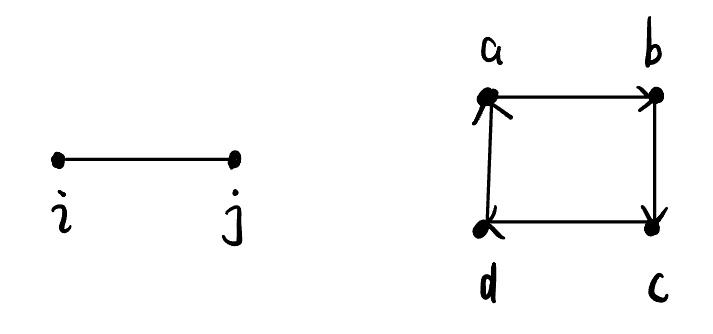
\includegraphics[width=0.35\linewidth]{images/period-2.jpg}
        \caption{左：无向二部图；右：有向环}
        \label{srr-fig:period-1}
    \end{figure}

    举例：图 \ref{srr-fig:period-1}（左）中状态$i$的周期为$\textup{gcd}\{2,4,6,8,\dots\}=2$，因此$i$的周期为$2$；类似地，$j$的周期也为$2$。
        
    \begin{definition}[非周期性]
        \label{defn:aperiodicity}
        若状态$i$的周期为$1$，则状态$i$是非周期性的（aperiodic）。若马尔可夫链中所有的状态都是非周期性的，则这个马尔科夫链是非周期性的。
    \end{definition}

    \textbf{关于周期性的更多例子}
    \begin{itemize}
        \item 无向二部图中状态（即图中顶点）的周期为$2$，例如图 \ref{srr-fig:period-1}（左）；
        \item 长为$k>1$的有向环中点的周期为$k$，例如图 \ref{srr-fig:period-1}（右）；
        \item 周期性阻止概率分布收敛到单一极限分布：
        \begin{itemize}
            \item 例如图 \ref{srr-fig:period-1}（左）中初始状态为$i$的马尔科夫链，奇数步后在$j$，偶数步后在$i$，因此概率分布会在两个分布之间振荡，无法收敛到单一极限。
        \end{itemize}
    \end{itemize}

    \begin{proposition}[可达性结果（Reachability Result）]
        \label{proposition:re-re}
        在任意有限（状态集合有限）、不可约、非周期的马尔可夫链中，存在$\tau<\infty$满足对于所有的$i,j$和$t\ge \tau$有：
        \[
            \Pr[X_t=j\mid X_0=i]>0.
        \]
    \end{proposition}

    注意：仅仅有限、不可约这两个条件不能得出性质 \ref{proposition:re-re} 中的结果。例如针对图 \ref{srr-fig:period-1}（左），其满足有限和不可约，但在$t$为奇数时，$\Pr[X_t=i|X_0=i]=0$，在$t$为偶数时，$\Pr[X_t=j|X_0=i]=0$。即因为周期性，导致某些时刻概率恒为$0$，不满足性质 \ref{proposition:re-re} 中的结果，因此需要“非周期”这个条件。



    \subsubsection{马尔科夫链基本定理}
        
    \begin{definition}[稳态分布]
        \label{defn:stationary-distribution}
        一个概率向量$\vec{\pi}\in\mathbb{R}^n$对于$P$是稳态分布（stationary distribution），如果满足：$\vec{\pi}P=\vec{\pi}$。
    \end{definition}

    \begin{itemize}
        \item $\vec{\pi}$是$P$的左特征向量，对应的特征值为$1$；
        \item 如果$\vec{\pi}$是稳态分布，那么对于所有的$t>0$有$\vec{\pi}P^t=\vec{\pi}$：
        \begin{itemize}
            \item $\vec{\pi}P^t=\vec{\pi}P\cdot P^{t-1}=\vec{\pi}P^{t-1}=\vec{\pi}P\cdot P^{t-2}=\vec{\pi}P^{t-2}=\cdots=\vec{\pi}$。
        \end{itemize}
    \end{itemize}

    \begin{definition}[TV距离]
        \label{defn:tv-distance}
        两个概率分布$\vec{p},\vec{q}\in\mathbb{R}^n$之间的TV距离（total variation distance）定义为
        \[
            d_{\textup{TV}}(\vec{p},\vec{q}):=\frac{1}{2}\sum_{i=1}^n{|p(i)-q(i)|}=\frac{1}{2}\lVert \vec{p}-\vec{q}\rVert_1.
        \]
    \end{definition}

    如果在$t\rightarrow \infty$时有$d_{\textup{TV}}(\vec{p}_t,\vec{q})\rightarrow 0$，则称$\vec{p}_t$（定义 \ref{defn:probability-distribution}）收敛于$\vec{q}$。

    \begin{theorem}[马尔科夫链基本定理] 
        \label{thrm:fund-mc}
        令$P\in \mathbb{R}^{n\times n}$定义一个有限、不可约、非周期的马尔科夫链。则对任意的初始分布$\vec{p}_0$，其对应的$\vec{p}_t:=\vec{p}_0P^t$在$t\rightarrow \infty$时收敛于一个唯一的稳态分布$\vec{\pi}$。
    \end{theorem}

    定理 \ref{thrm:fund-mc} 针对所有满足有限、不可约、非周期的马尔科夫链成立，而无向图上的随机游走是特殊的马尔科夫链，接下来我们运用谱分析证明一个特殊版本（关于无向图上的随机游走）的马尔可夫链基本定理。


        
\subsection{无向图上的简单随机游走}
        
本节我们考虑无向图上的随机游走，这是一种特殊的马尔科夫链，希望运用谱图论证明定理 \ref{thrm:fund-mc}。

\textbf{一些基础符号。}针对无权无向图$G=(V,E)$，$A\in\mathbb{R}^{n\times n}$表示图$G$的邻接矩阵，$D\in\mathbb{R}^{n\times n}$表示度数对角矩阵，其中$D_{ii}=\textup{deg}(i)$。

\vspace{0.2cm}
回忆无权无向图$G=(V,E)$上的随机游走是指从图中某个点出发，在每一步，从当前所在点的邻居中均匀随机地选择一个点进行移动（游走）。
        
\begin{itemize}
    \item 令$P_{ij}$表示从点$i$到点$j$的单步转移概率，则：
    \begin{itemize}
        \item 若$(i,j)\in E$，有$P_{ij}=\frac{1}{\textup{deg}(i)}$；
        \item 若$(i,j)\notin E$，有$P_{ij}=0$；
    \end{itemize}
    \item 因此\textcolor{blue}{转移矩阵$P=D^{-1}A$}。这称为图上简单随机游走的转移矩阵。
    \item 令$\bm{p}_0:V\rightarrow \mathbb{R}$表示初始概率分布，则$\bm{p}_{t+1} = \bm{p}_t P= \bm{p}_t D^{-1}A
        \quad \Rightarrow \quad
        \textcolor{blue}{\bm{p}_t = \bm{p}_0 (D^{-1}A)^t}.$
\end{itemize}

\vspace{0.2cm}
类似定义 \ref{defn:stationary-distribution}，我们定义$\bm{\pi}:V\to \mathbb{R}$为稳态分布，如果$\bm{\pi}$满足$\bm{\pi}P=\bm{\pi}$。$\bm{\pi}$是$P$的左特征向量，对应的特征值为$1$。%针对$P=D^{-1}A$，一个自然的稳态分布$\bm{\pi}$可以定义为$\bm{\pi}(i)=\frac{\textup{deg}(i)}{2|E|}$。

\begin{lemma}
    \label{lemma:sta-dist-graoh}
    令$G=(V,E)$表示一个无向图，令$P=D^{-1}A$。对所有$i\in V$，定义
    \[
        \bm{\pi}(i)=\frac{\textup{deg}(i)}{2|E|},
    \]
    则$\bm{\pi}$是$P$的一个稳态分布。
            
    \begin{proof}
        \begin{align*}
            \bm{\pi}P&=\bm{\pi}D^{-1}A\\
            &=\frac{1}{2|E|}\vec{1}\cdot  A\\
            &=\frac{1}{2|E|}\left(\textup{deg}(1),\dots,\textup{deg}(n)\right)\\
            &=\bm{\pi}.
        \end{align*}
    \end{proof}
\end{lemma}

定理 \ref{thrm:fund-mc} 中马尔科夫链需要满足有限、不可约、非周期三个条件。因此我们需要在图上对应有限、不可约、非周期三个条件。

\paragraph{有限。}只要图上的顶点数$|V|$有限就满足了“有限”这个条件。

\paragraph{不可约。}若$G$是不连通的，则随机游走的长期表现（long-term behavior）取决于起始点，稳态分布也不是唯一的。
        
考虑图$G$中有两个连通分量$G_1=(V_1,E_1)$和$G_2=(V-V_1,E-E_1)$：
\begin{itemize}
    \item 若起始点为$G_1$中的点（即$V_1$中的点），则稳态分布为
    \begin{itemize}
        \item 对$i\in V_1$，$\bm{\pi}(i)=\frac{\textup{deg}(i)}{2|E_1|}$；
        \item 对$i\notin V_1$，$\bm{\pi}(i)=0$；
    \end{itemize}

    \item 若起始点为$G_2$中的点（即$V-V_1$中的点），则稳态分布为
    \begin{itemize}
        \item 对$i\notin V_1$，$\bm{\pi}(i)=\frac{\textup{deg}(i)}{2|E-E_1|}$；
        \item 对$i\in V_1$，$\bm{\pi}(i)=0$。
    \end{itemize}
\end{itemize}

\begin{fact}
    \label{fact:irre-graph}
    当且仅当$G$连通时，不可约条件满足。
\end{fact}

\paragraph{非周期。}即使在连通图中，随机游走也可能不会收敛到一个稳态分布，例如图 \ref{srr-fig:period-1} （左）中的连通二部图，其概率分布会在两个分布之间振荡，无法收敛到单一极限。

\begin{fact}
    \label{fact:aper-graph}
    当且仅当$G$是非二部图（non-bipartite）时，非周期条件满足。
\end{fact}



    \subsubsection{特殊的马尔科夫链基本定理}
        
    结合事实 \ref{fact:irre-graph}、事实 \ref{fact:aper-graph} 和引理 \ref{lemma:sta-dist-graoh}，我们想要证明的特殊版本的定理 \ref{thrm:fund-mc} 变为以下定理：

    \begin{theorem}
        \label{thrm:special-fund-mc}
        令$G$表示一个无向、连通的非二部图，并且转移矩阵$P=D^{-1}A$，则满足以下定义的分布$\bm{\pi}$是\textbf{唯一}的稳态分布：
        \[
            \bm{\pi}(i)=\frac{\textup{deg}(i)}{2|E|}.
        \]
        即对任意的初始分布$\bm{p}_0$，其对应的$\bm{p}_t=\bm{p}_0P^t$在$t\to \infty$时收敛于$\bm{\pi}$%，即$\bm{p}_t=\bm{p}_0P^t\to \bm{\pi}$
            。
    \end{theorem}
        


\subsection{$d$-正则非二部图上的简单随机游走}

    接下来我们的目标是使用\textbf{谱分析（spectral analysis）}证明上节中给出的特殊的马尔可夫链基本定理（定理 \ref{thrm:special-fund-mc}），即证明随机游走会收敛到一个唯一的稳态分布。此外谱技巧（spectral techniques）可以精确分析混合时间（mixing time），即收敛速度。 本节首先考虑在一类特殊的图（$d$-正则非二分图）上进行证明，在后面章节推广到更一般的图上。

    对$d$-正则图：
    \begin{itemize}
        \item 简单随机游走的转移矩阵$P=D^{-1}A=\frac{1}{d}A=\mathcal{A}$；
        \begin{itemize}
            \item $\mathcal{A}$为正则化的邻接矩阵；
        \end{itemize}
        \item $P$为实对称矩阵，因此特征值都是实数；
        \item 稳态分布满足$\bm{\pi}(i)=\frac{d}{dn}=\frac{1}{n}$，因此$\bm{\pi}=\frac{\bm{1}}{n}$。
    \end{itemize}

    \vspace{0.2cm}
    \textbf{$P=\mathcal{A}$的谱性质。}令$\alpha_1\ge \alpha_2\ge \dots\ge \alpha_n$表示$\mathcal{A}$的特征值，对应的一组标准正交特征向量为$v_1,v_2,\dots,v_n$：
    \begin{itemize}
        \item 由Notes Lec 10中引理 28 可知，$\alpha_1=1$，且$v_1=\frac{\bm{1}}{\sqrt{n}}$；
        \item \textcolor{blue}{当且仅当$G$是连通图时，$\alpha_2<1$}；
            \begin{itemize}
                \item 由Notes Lec 10中引理 22 可知，当且仅当$G$是连通图时，$L=D-A$的第二小特征值$\lambda_2>0$（对应的特征向量为$v_2$），可以验证$\alpha_i=1-\frac{\lambda_i}{d}$，因此$\alpha_2=1-\frac{\lambda_2}{d}<1$；
            \end{itemize}
        \item \textcolor{blue}{当且仅当$G$是非二部图时，$\alpha_n>-1$}（当且仅当$G$是二部图时，$\alpha_n=-1$）；
            \begin{itemize}
                \item 由Notes Lec 10中引理 12 可得。
            \end{itemize}
        \end{itemize}

    \vspace{0.25cm}
    下面给出与定理 \ref{thrm:special-fund-mc} 相对应的$d$-正则非二部图上的结论，即定理 \ref{thrm:fund-mc-d-1}。
            
    \begin{theorem}
        \label{thrm:fund-mc-d-1}
        令$G$表示一个$d$-正则化的、无向、连通的非二部图，简单随机游走的转移矩阵$P=D^{-1}A=\mathcal{A}$，那么对于所有的初始概率分布$\bm{p}_0$：
        \[
            \lim_{t \to \infty} \bm{p}_0\mathcal{A}^t  = \frac{\bm{1}}{n}.
        \]
    \end{theorem}

    \begin{proof}
        % 因为$\mathcal{A}$的特征向量$v_1,\dots,v_n$构成一组标准正交基，因此任意的初始向量$\bm{p}_0$都可以用$v_1,\dots,v_n$表示，即$\bm{p}_0=\sum_{i=1}^n{c_iv_i^{\top}}$，其中$c_1,\dots,c_n$为常数。
                    
        % 此外，
        $\mathcal{A}$的特征分解可以表示为$\mathcal{A}=\sum_{i=1}^n{\alpha_iv_iv_i^{\top}}$。由于$v_1,\dots,v_n$构成一组标准正交基，则对任意$i\ne j$有$v_i^{\top}v_j=0$，对任意$i\in[n]$有$v_i^{\top}v_i=1$。因此$\mathcal{A}^t=\sum_{i=1}^n{\alpha_i^tv_iv_i^{\top}}$。

        \begin{align*}
            \bm{p}_0\mathcal{A}^t&=\bm{p}_0\sum_{i=1}^n{\alpha_i^tv_iv_i^{\top}}\\
            &=\bm{p}_0\cdot \alpha_1^tv_1v_1^{\top}+\bm{p}_0\sum_{i=2}^n{\alpha_i^tv_iv_i^{\top}}\\
            &=\frac{\bm{1}}{n}+\bm{p}_0\sum_{i=2}^n{\alpha_i^tv_iv_i^{\top}}&&\text{（$\alpha_1=1,v_1=\frac{\bm{1}}{\sqrt{n}}$且$\bm{p}_0$满足$\sum_{i=1}^n\bm{p}_0(i)=1$）}
        \end{align*}

        等式两边同时取极限，可得：
                    
        \begin{align*}
            \lim_t \bm{p}_0\mathcal{A}^t =\lim_t \frac{\bm{1}}{n}+\bm{p}_0\sum_{i=2}^n{\alpha_i^tv_iv_i^{\top}}=\frac{\bm{1}}{n},
        \end{align*}
        
        这是因为在连通的非二部图中，$1>\alpha_2\ge \alpha_3\ge \dots\ge \alpha_n>-1$，因此在$t\to \infty$时，$\forall i>1$，${|\alpha_i^t|}\to 0$，即$\bm{p}_0\sum_{i=2}^n{\alpha_i^tv_iv_i^{\top}}\to 0$。
                    
    \end{proof}

    马尔科夫链基本定理表明在步数$t\to \infty$时，随机游走的概率分布趋于稳态分布。现在我们关心$t$足够大时，随机游走概率分布的表现，而不是$t\to \infty$时。因此我们引入混合时间（mixing time）的概念。

    \begin{definition}[混合时间]
        \label{defn:mixing-time}
        对于转移矩阵为$P$的随机游走，令$\bm{p}_t=\bm{p}_0P^t$表示从初始分布$\bm{p}_0$开始的步长为$t$的随机游走的概率分布，$\bm{\pi}=\lim_{t \to \infty} \bm{p}_t$表示稳态分布。混合时间$\tau_{\varepsilon}(P)$定义为对任意初始分布$\bm{p}_0$，满足$d_{\textup{TV}}(\bm{p}_t,\bm{\pi})\le \varepsilon$的最小的步数$t$。
    \end{definition}

    在本节中，除非$\varepsilon$被特殊指明，否则我们默认$\varepsilon=1/4$。接下来我们给出简单随机游走混合时间的上界。%与上节类似，我们首先在一类特殊的图（$d$-正则图）上给出混合时间的上界（更简单），其次在更一般的图上给出混合时间的上界。

    回忆在$d$-正则图上，$P=D^{-1}A=\frac{1}{d}A=\mathcal{A}$，$W=\frac{1}{2}I+\frac{1}{2}P=\frac{1}{2}I+\frac{1}{2}\mathcal{A}$。$1=\alpha_1\ge \alpha_2\ge\dots \ge \alpha_n\ge -1$表示$\mathcal{A}$的特征值，对应的一组标准正交的特征向量为$v_1,\dots,v_n$。稳态分布为$\bm{\pi}=\frac{\bm{1}}{n}$。

    定义\textbf{谱间隔（spectral gap）}为$g:=\min\{1-\alpha_2,1-|\alpha_n|\}$。

    \paragraph{通过谱间隔给出混合时间的上界：}

    \begin{fact}
        \label{fact:norm}
        对任意向量$x\in\mathbb{R}^n$，有$\lVert x\rVert_1\le \sqrt{n}\lVert x\rVert_2$。
        \begin{proof}
            利用柯西不等式：
            \begin{align*}
                \lVert x\rVert_1=\sum_{i=1}^n{|x(i)|}
                \le \sqrt{\left(\sum_{i=1}^n{1^2}\right)\left(\sum_{i=1}^n{x(i)^2}\right)}
                =\sqrt{n}\cdot \lVert x\rVert_2.
            \end{align*}
        \end{proof}
    \end{fact}
                
    \begin{theorem}
        \label{thrm:mixing-time-d-sg}
        令$G$表示一个无向、连通、非二部图的$d$-正则图，$P=\mathcal{A}$为图上的简单随机游走转移矩阵。则$\tau_{\varepsilon}(P)\lesssim\frac{1}{g}\ln{\left(\frac{n}{\varepsilon}\right)}$。
    \end{theorem}

    注：$a \lesssim b$中$\lesssim$符号隐藏了常数，表示$a\le c\cdot b$，其中$c$是一个常数。可以认为$\lesssim$符号与$O$符号类似。

    定理 \ref{thrm:mixing-time-d-sg} 表明无向、连通、非二部图（连通的非二部图的$g>0$）的$d$-正则图上简单随机游走的混合时间与谱间隔$g$有关。

    \begin{proof}
        因为$\mathcal{A}$的特征向量$v_1,\dots,v_n$（列向量）构成一组标准正交基，因此任意的初始向量$\bm{p}_0$（行向量）都可以用$v_1,\dots,v_n$表示，即$\bm{p}_0=\sum_{i=1}^n{c_iv_i^{\top}}$，其中$c_1,\dots,c_n$为常数。此外，$P=\mathcal{A}=\sum_{i=1}^n{\alpha_iv_iv_i^{\top}}$，且$P^t=\mathcal{A}^t=\sum_{i=1}^n{\alpha_i^tv_iv_i^{\top}}$。%则$\bm{p}_t=\bm{p}_0P^t=\sum_{i=1}^n{c_i\alpha_i^tv_i^{\top}}$。
        
        由定理 \ref{thrm:fund-mc-d-1} 的证明可知$\bm{p}_t=\bm{p}_0P^t=\frac{\bm{1}}{n}+\bm{p}_0\sum_{i=2}^n{\alpha_i^tv_iv_i^{\top}}$，因此
                    
        \begin{align*}
            d_{\textup{TV}}(\bm{p}_t,\bm{\pi})&=\frac{1}{2}\lVert \bm{p}_t-\bm{\pi} \rVert_1\\
            % &\le \lVert \bm{p}_t-\bm{\pi} \rVert_1\\
            &=\frac{1}{2}\lVert \frac{\bm{1}}{n}+\bm{p}_0\sum_{i=2}^n{\alpha_i^tv_iv_i^{\top}}-\frac{\bm{1}}{n}\rVert_1\\
            &=\frac{1}{2}\lVert \bm{p}_0\sum_{i=2}^n{\alpha_i^tv_iv_i^{\top}}\rVert_1\\
            &=\frac{1}{2}\lVert \sum_{i=2}^n{c_i\alpha_i^tv_i^{\top}}\rVert_1&&\text{($\bm{p}_0=\sum_{i=1}^n{c_iv_i^{\top}}$)}\\
            &\le \frac{\sqrt{n}}{2}\lVert \sum_{i=2}^n{c_i\alpha_i^tv_i^{\top}}\rVert_2&&\text{（事实 \ref{fact:norm}）}.
        \end{align*}

        令向量$X=\sum_{i=2}^n{c_i\alpha_i^tv_i^{\top}}$，则$X(k)=\sum_{i=2}^n{c_i\alpha_i^tv_i(k)}$，因此
        
        \begin{align*}
            \lVert \sum_{i=2}^n{c_i\alpha_i^tv_i^{\top}}\rVert_2^2&=\lVert X\rVert_2^2\\
            &=\sum_{k=1}^n{X(k)^2}\\
            &=\sum_{k=1}^n{\left(\sum_{i=2}^n{c_i\alpha_i^tv_i(k)}\right)^2}\\
            &=\sum_{k=1}^n{\left(\sum_{i=2}^n{\sum_{j=2}^n{c_i\alpha_i^tv_i(k)\cdot c_j\alpha_j^tv_j(k)}}\right)}\\
            &=\sum_{i=2}^n{\sum_{j=2}^n{c_i\alpha_i^tc_j\alpha_j^t\sum_{k=1}^n{v_i(k)v_j(k)}}}\\
            &=\sum_{i=2}^n{c_i^2\alpha_i^{2t}}&&\text{（$v_1,\dots,v_n$是一组标准正交基）}\\
            &\le (1-g)^{2t}\sum_{i=2}^n{c_i^2}\\
            &\le e^{-2gt}\sum_{i=2}^n{c_i^2}.
        \end{align*}

        结合上面两个式子，有：
        
        \begin{align*}
            d_{\textup{TV}}(\bm{p}_t,\bm{\pi})&\le \frac{\sqrt{n}}{2}\lVert \sum_{i=2}^n{c_i\alpha_i^tv_i^{\top}}\rVert_2\\
            &\le\frac{\sqrt{n}}{2}\sqrt{e^{-2gt}\sum_{i=2}^n{c_i^2}}\\
            &\le\frac{\sqrt{n}}{2}\sqrt{e^{-2gt}\sum_{i=1}^n{c_i^2}}\\
            &=\frac{\sqrt{n}}{2}\sqrt{e^{-2gt}\left\|p_0\right\|_2^2}\\
            &\le\frac{\sqrt{n}}{2}\sqrt{e^{-2gt}\left\|p_0\right\|_1}\\
            &=\frac{\sqrt{n}}{2}e^{-gt}\\
            &=\frac{\sqrt{n}}{2}e^{-g\cdot C\frac{1}{g}\ln{\left(\frac{n}{\varepsilon}\right)}}&&\text{（$t=\tau_{\varepsilon}(P)\lesssim\frac{1}{g}\ln{\left(\frac{n}{\varepsilon}\right)}$）}\\
            &=\frac{\sqrt{n}}{2}\left(\frac{\varepsilon}{n}\right)^{C}\\
            &\le \varepsilon.&&\text{（取足够大的$C\ge 1$）}\\
            %&\lesssim \sqrt{n}e^{-tg}.
        \end{align*}
    \end{proof}

    

            
\subsection{$d$-正则图上的懒惰随机游走}

\paragraph{去掉非周期性条件。}定理 \ref{thrm:special-fund-mc} 中的非二部图保证了马尔可夫链是非周期的（事实 \ref{fact:aper-graph}）。若想移除非二部图这个条件，我们可以给图上的点加自环（self-loops）。这将引出懒惰随机游走（lazy random walk）的概念。本节中我们首先研究$d$-正则非二分图上的懒惰随机游走。

\begin{definition}[（$d$-正则图上的）懒惰随机游走]
    \label{defn:lazy-random-walk-regular}
    给定一个$d$-正则无向图$G$，其上的懒惰随机游走对应的转移矩阵$W$定义为：\[W=\frac{1}{2}I+\frac{A}{2d}.\]
\end{definition}

直观上看，图上的懒惰随机游走从某个点开始，在每一步，以$\frac{1}{2}$的概率留在原地，以$\frac{1}{2}$的概率随机均匀随机地选择一个邻居进行转移（游走）。

考虑懒惰随机游走的好处：
\begin{itemize}
    \item 加自环打破了二部图的周期性；
    \item 这种修改确保马尔可夫链变为非周期性的，同时不会显著改变图的结构。
\end{itemize}

\iffalse
\begin{corollary}
    \label{coro:fund-mc-lazy}
    令$G$表示一个无向、连通图。令$W=\frac{1}{2}I+\frac{1}{2}D^{-1}A$表示懒惰随机游走的转移矩阵。则满足以下定义的分布$\bm{\pi}$是\textbf{唯一}的稳态分布：
    \[
        \bm{\pi}(i)=\frac{\textup{deg}(i)}{2|E|}.
    \]
    即对任意的初始分布$\bm{p}_0$，其对应的$\bm{p}_t=\bm{p}_0W^t$在$t\to \infty$时收敛于$\bm{\pi}$%，即$\bm{p}_t=\bm{p}_0W^t\to \bm{\pi}$
    。
\end{corollary}
\fi

首先分析懒惰随机游走转移矩阵$W$的谱性质。
            
\vspace{0.2cm}
\textbf{$W$的谱性质。}由$W=\frac{1}{2}I+\frac{1}{2}\mathcal{A}$可知，$W$的特征值为$\frac{1}{2}(1+\alpha_i)$，对应的特征向量为$v_i$。$W$的特征值$\frac{1}{2}(1+\alpha_i)$有以下规律：
\begin{itemize}
    \item $W$的最大特征值为$\frac{1}{2}(1+\alpha_1)=1$；
    \item 因为$\alpha_i\ge -1$，因此对所有$i\in[n]$，$W$的特征值$\frac{1}{2}(1+\alpha_i)\ge 0$；
    \item $1> \frac{1+\alpha_2}{2}\ge \dots\ge \frac{1+\alpha_n}{2}\ge 0$。
\end{itemize}
            
下面给出$d$-正则非二分图上的稳态分布，即定理 \ref{thrm:fund-mc-d-2}。

\begin{theorem}
    \label{thrm:fund-mc-d-2}
    令$G$表示一个$d$-正则化的、无向、连通图，转移矩阵$W=\frac{1}{2}I+\frac{1}{2}\mathcal{A}$，那么对于所有的初始概率分布$\bm{p}_0$：
    \[
        \lim_{t \to \infty} \bm{p}_0W^t  = \frac{\bm{1}}{n}.
    \]
\end{theorem}

\begin{proof}
    （证明与定理 \ref{thrm:fund-mc-d-1} 类似。）由$W$的谱性质可知，$W$的特征值为$\frac{1}{2}(1+\alpha_i)$，对应的特征向量为$v_i$，因此$W$的特征分解可以表示为$W=\sum_{i=1}^n{\frac{1+\alpha_i}{2}v_iv_i^{\top}}$，类似地，$W^t=\sum_{i=1}^n{\left(\frac{1+\alpha_i}{2}\right)^tv_iv_i^{\top}}$。
    \begin{align*}
        \bm{p}_0W^t&=\bm{p}_0\sum_{i=1}^n{\left(\frac{1+\alpha_i}{2}\right)^tv_iv_i^{\top}}\\
        &=\bm{p}_0\left(\frac{1+\alpha_1}{2}\right)v_1v_1^{\top}+\bm{p}_0\sum_{i=2}^n{\left(\frac{1+\alpha_i}{2}\right)^tv_iv_i^{\top}}\\
        &=\frac{\bm{1}}{n}+\bm{p}_0\sum_{i=2}^n{\left(\frac{1+\alpha_i}{2}\right)^tv_iv_i^{\top}}&&\text{（$\alpha_1=1,v_1=\frac{\bm{1}}{\sqrt{n}}$且$\bm{p}_0$满足$\sum_{i=1}^n\bm{p}_0(i)=1$）}
    \end{align*}

    等式两边同时取极限，可得：
    \begin{align*}
        \lim_t \bm{p}_0W^t =\lim_t \left(\frac{\bm{1}}{n}+\bm{p}_0\sum_{i=2}^n{\left(\frac{1+\alpha_i}{2}\right)^tv_iv_i^{\top}}\right)=\frac{\bm{1}}{n},
    \end{align*}
    
    这是因为在连通图中，$1>\alpha_2\ge \alpha_3\ge \dots\ge \alpha_n>-1$，因此$1> \frac{1+\alpha_2}{2}\ge \dots\ge \frac{1+\alpha_n}{2}\ge 0$。则在$t\to \infty$时，$\forall i>1$，${|\left(\frac{1+\alpha_i}{2}\right)^t|}\to 0$，即$\bm{p}_0\sum_{i=2}^n{\left(\frac{1+\alpha_i}{2}\right)^tv_iv_i^{\top}}\to 0$。
\end{proof}

\paragraph{通过导率（conductance）给出混合时间的上界：}
                
回忆在$d$-正则图上，懒惰随机游走的转移矩阵$W=\frac{1}{2}I+\frac{1}{2}P=\frac{1}{2}I+\frac{1}{2}\mathcal{A}$，$W$的特征值为$\frac{1}{2}(1+\alpha_i)$，均$\ge 0$。稳态分布为$\bm{\pi}=\frac{\bm{1}}{n}$。此外，图$G$的正则化拉普拉斯矩阵$\mathcal{L}=I-\frac{A}{d}=I-\mathcal{A}$，特征值为$0\le\lambda_1\le \lambda_2\le\dots\le \lambda_n\le 2$（对应的特征向量为$v_1,\dots,v_n$），其中$\lambda_i=1-\alpha_i$。

定义\textbf{谱间隔（spectral gap）}为$g:=\frac{1}{2}(1-\alpha_2)=\frac{1}{2}\lambda_2$。

\begin{theorem}
    \label{thrm:mixing-time-d-c}
    令$G$表示一个无向、连通的$d$-正则图，$W=\frac{1}{2}I+\frac{1}{2}\mathcal{A}$为图上的懒惰随机游走转移矩阵。则$\tau_{\varepsilon}(W)\lesssim\frac{1}{\phi(G)^2}\ln{\left(\frac{n}{\varepsilon}\right)}$。
\end{theorem}

定理 \ref{thrm:mixing-time-d-c} 表明无向、连通（连通图的$g>0$，即$\phi(G)>0$）的$d$-正则图上懒惰随机游走的混合时间与导率$\phi(G)$有关。

\begin{proof}
    （总体证明思路与定理 \ref{thrm:mixing-time-d-sg} 的证明类似，最后用到Cheeger不等式。）

    由定理 \ref{thrm:fund-mc-d-2} 的证明可知$\bm{p}_t=\bm{p}_0W^t=\frac{\bm{1}}{n}+\bm{p}_0\sum_{i=2}^n{\left(\frac{1+\alpha_i}{2}\right)^tv_iv_i^{\top}}$，因此

    \[
        d_{\textup{TV}}(\bm{p}_t,\bm{\pi})\le \frac{\sqrt{n}}{2}\lVert \sum_{i=2}^n{c_i\left(\frac{1+\alpha_i}{2}\right)^tv_i^{\top}}\rVert_2.
    \]
                    % \begin{align*}
                    %     d_{\textup{TV}}(\bm{p}_t,\bm{\pi})&=\frac{1}{2}\lVert \bm{p}_t-\bm{\pi} \rVert_1\\
                    %     % &\le \lVert \bm{p}_t-\bm{\pi} \rVert_1\\
                    %     &=\frac{1}{2}\lVert \frac{\bm{1}}{n}+\bm{p}_0\sum_{i=2}^n{\left(\frac{1+\alpha_i}{2}\right)^tv_iv_i^{\top}}-\frac{\bm{1}}{n}\rVert_1\\
                    %     &=\frac{1}{2}\lVert \bm{p}_0\sum_{i=2}^n{\left(\frac{1+\alpha_i}{2}\right)^tv_iv_i^{\top}}\rVert_1\\
                    %     &=\frac{1}{2}\lVert \sum_{i=2}^n{c_i\left(\frac{1+\alpha_i}{2}\right)^tv_i^{\top}}\rVert_1&&\text{($\bm{p}_0=\sum_{i=1}^n{c_iv_i^{\top}}$)}\\
                    %     &\le \frac{\sqrt{n}}{2}\lVert \sum_{i=2}^n{c_i\left(\frac{1+\alpha_i}{2}\right)^tv_i^{\top}}\rVert_2&&\text{（事实 \ref{fact:norm}）}.
                    % \end{align*}

    此外，
    
    \begin{align*}
        \lVert \sum_{i=2}^n{c_i\left(\frac{1+\alpha_i}{2}\right)^tv_i^{\top}}\rVert_2^2&=\sum_{i=2}^n{c_i^2\left(\frac{1+\alpha_i}{2}\right)^{2t}}\\
        &=\sum_{i=2}^n{c_i^2\left(1-\frac{\lambda_i}{2}\right)^{2t}}&&\text{（$\lambda_i=1-\alpha_i$）}\\
        &\le (1-g)^{2t}\sum_{i=1}^n{c_i^2}\\
        &\le e^{-2gt}\sum_{i=2}^n{c_i^2}.
    \end{align*}
                    % 令向量$X=\sum_{i=2}^n{c_i\left(\frac{1+\alpha_i}{2}\right)^tv_i^{\top}}$，则$X(k)=\sum_{i=2}^n{c_i\left(\frac{1+\alpha_i}{2}\right)^tv_i(k)}$，因此
                    % \begin{align*}
                    %     \lVert \sum_{i=2}^n{c_i\left(\frac{1+\alpha_i}{2}\right)^tv_i^{\top}}\rVert_2^2&=\lVert X\rVert_2^2\\
                    %     &=\sum_{k=1}^n{X(k)^2}\\
                    %     &=\sum_{k=1}^n{\left(\sum_{i=2}^n{c_i\left(\frac{1+\alpha_i}{2}\right)^tv_i(k)}\right)^2}\\
                    %     &=\sum_{k=1}^n{\left(\sum_{i=2}^n{\sum_{j=2}^n{c_i\left(\frac{1+\alpha_i}{2}\right)^tv_i(k)\cdot c_j\left(\frac{1+\alpha_j}{2}\right)^tv_j(k)}}\right)}\\
                    %     &=\sum_{i=2}^n{\sum_{j=2}^n{c_i\left(\frac{1+\alpha_i}{2}\right)^tc_j\left(\frac{1+\alpha_j}{2}\right)^t\sum_{k=1}^n{v_i(k)v_j(k)}}}\\
                    %     &=\sum_{i=2}^n{c_i^2\left(\frac{1+\alpha_i}{2}\right)^{2t}}&&\text{（$v_1,\dots,v_n$是一组标准正交基）}\\
                    %     &\le (1-g)^{2t}\sum_{i=2}^n{c_i^2}\\
                    %     &\le e^{-2gt}\sum_{i=2}^n{c_i^2}.
                    % \end{align*}

    结合上面两个式子，有：
    
    \begin{align*}
        d_{\textup{TV}}(\bm{p}_t,\bm{\pi})&\le \frac{\sqrt{n}}{2}\lVert \sum_{i=2}^n{c_i\left(\frac{1+\alpha_i}{2}\right)^tv_i^{\top}}\rVert_2\\
        &\le\frac{\sqrt{n}}{2}\sqrt{e^{-2gt}\sum_{i=2}^n{c_i^2}}\\
        &\le\frac{\sqrt{n}}{2}\sqrt{e^{-2gt}\sum_{i=1}^n{c_i^2}}\\
            &=\frac{\sqrt{n}}{2}\sqrt{e^{-2gt}\left\|p_0\right\|_2^2}\\
            &\le\frac{\sqrt{n}}{2}\sqrt{e^{-2gt}\left\|p_0\right\|_1}\\
            &=\frac{\sqrt{n}}{2}e^{-gt}\\
            &=\frac{\sqrt{n}}{2}e^{-g\cdot C\frac{1}{g}\ln{\left(\frac{n}{\varepsilon}\right)}}&&\text{（$t=\tau_{\varepsilon}(P)\lesssim\frac{1}{g}\ln{\left(\frac{n}{\varepsilon}\right)}$）}\\
            &=\frac{\sqrt{n}}{2}\left(\frac{\varepsilon}{n}\right)^{C}\\
            &\le \varepsilon.&&\text{（取足够大的$C\ge 1$）}\\
        %&\lesssim \sqrt{n}e^{-tg}.
    \end{align*}
                    
    由Notes Lec 14中的Cheeger不等式可知$\frac{\lambda_2}{2}\le \phi(G)\le \sqrt{2\lambda_2}$，因此$\lambda_2\ge \frac{\phi(G)^2}{2}$，$g=\frac{1}{2}\lambda_2\ge \frac{\phi(G)^2}{4}$，因此$\tau_{\varepsilon}(W)\le C_2\frac{1}{g}\ln{\left(\frac{n}{\varepsilon}\right)}\le 4C_2 \frac{1}{\phi(G)^2}\ln{\left(\frac{n}{\varepsilon}\right)}$，即$\tau_{\varepsilon}(W)\lesssim  \frac{1}{\phi(G)^2}\ln{\left(\frac{n}{\varepsilon}\right)}$。
\end{proof}

\textbf{应用：}对于扩展图（expanders）$G$，其导率满足$\phi(G)=\Omega(1)$，根据定理 \ref{thrm:mixing-time-d-c}，扩展图上的混合时间为$\tau_{\varepsilon}(W)=O(\log n)$，这一结论在以下场景下有用：
    \begin{itemize}
        \item 均匀采样；
        \item 设计随机化算法（randomized algorithms）；
        \item 快速混合马尔科夫链。
    \end{itemize}

总结：通过给图加自环、分析新图上懒惰随机游走可以简化分析。此外，加自环不会显著影响图上随机游走的性质。

            


\subsection{一般非二部图上的简单随机游走}

本节我们首先证明一般图上的马尔科夫链基本定理。其次给出一般图上的混合时间的上界。我们依然首先关心非二部图的情况。

\vspace{0.2cm}
对一般图：
\begin{itemize}
    \item 简单随机游走的转移矩阵$P=D^{-1}A$；
    \item 由于图不一定是$d$-正则图，因此$P$不一定是对称矩阵；
    \begin{itemize}
        \item 因此，谱定理（Notes Lec 10中的定理3）无法直接应用。
    \end{itemize}
\end{itemize}

\vspace{0.2cm}
\textbf{谱的相似性（spectral similarity）：}两个矩阵在谱性质上相似通常指它们的特征值/特征向量可以通过某种方式一一对应，且谱性质相近。如果两个矩阵$M,N$相似，即存在可逆矩阵$S$满足$M=S^{-1}NS$，则$M,N$具有相同的特征值（但特征向量可能不同）。
            
\vspace{0.2cm}
定义正则化邻接矩阵$\mathcal{A}=D^{-1/2}AD^{-1/2}$，可以验证$\mathcal{A}$一定为实对称矩阵。此时：
\begin{itemize}
    \item $P=D^{-1}A=D^{-1/2}\mathcal{A}D^{1/2}$，与$\mathcal{A}$相似，记为$P\sim \mathcal{A}$
    \item 根据谱的相似性，$P$的特征值与$\mathcal{A}$的特征值相同，均为实数。
\end{itemize}

\begin{lemma}
    \label{lemma:similarity-P}
    令$G$表示一个连通的无向图，其正则化邻接矩阵为$\mathcal{A}$。令$\alpha_1>\alpha_2\ge \dots\ge \alpha_n$表示$\mathcal{A}$的特征值，对应的一组标准正交特征向量为$v_1,\dots,v_n$，其中$v_1=\frac{1}{\sqrt{2|E|}}D^{1/2}\bm{1}$。
    则：
    \begin{itemize}
        \item $P=D^{-1}A$的特征值为$\alpha_1,\dots,\alpha_n$；
        \item $P$的特征向量为$D^{-1/2}v_1,\dots,D^{-1/2}v_n$。
    \end{itemize}
\end{lemma}

\begin{proof}
    利用谱的相似性依次证明：
    \begin{itemize}
        \item 由于$P\sim \mathcal{A}$，因此$P$与$\mathcal{A}$的特征值相同，为$\alpha_1,\dots,\alpha_n$；
        \item $PD^{-1/2}v_i=D^{-1/2}\mathcal{A}D^{1/2}D^{-1/2}v_i=D^{-1/2}\mathcal{A}v_i=D^{-1/2}\alpha_iv_i=\alpha_iD^{-1/2}v_i$。
    \end{itemize}
\end{proof}

注意$v_1,\dots,v_n$是一组标准正交基，即对于任意$i\ne j\in[n]$，有$\langle v_i,v_j\rangle=0$；对于任意$i\in[n]$，有$\lVert v_i\rVert_2=\sqrt{v_i^{\top}v_i} =1$。但$P$的特征向量$D^{-1/2}v_1,\dots,D^{-1/2}v_n$不一定是一组标准正交基。因此，我们定义带权重的内积：
\begin{itemize}
    \item $\langle u,v\rangle_{D}=u^{\top}Dv$；
    \item $\lVert v\rVert_{D}=\sqrt{v^{\top}Dv}$。
\end{itemize}

在带权重内积的度量下，$P$的特征向量$D^{-1/2}v_1,\dots,D^{-1/2}v_n$是一组标准正交基，即：
\begin{itemize}
    \item 对于任意$i\ne j\in[n]$，有$\langle D^{-1/2}v_i,D^{-1/2}v_j\rangle_D=0$；
    \item 对于任意$i\in[n]$，有$\Vert D^{-1/2}v_i\rVert_D =1$。
\end{itemize}

\vspace{0.25cm}
下面给出与定理 \ref{thrm:special-fund-mc}、定理 \ref{thrm:fund-mc-d-1} 相对应的一般图上的结论，即定理 \ref{thrm:fund-mc-g-1}。
            
\begin{theorem}
    \label{thrm:fund-mc-g-1}
    令$G$表示一个无向、连通的非二部图，简单随机游走的转移矩阵$P=D^{-1}A=D^{-1/2}\mathcal{A}D^{1/2}$，特征值为$1=\alpha_1>\alpha_2\ge\dots \ge \alpha_n> -1$。那么对于所有的初始概率分布$\bm{p}_0$：
    \[
        \lim_{t \to \infty} \bm{p}_0P^t  = \frac{\bm{d}}{2|E|},
    \]
    其中$\bm{d}\in \mathbb{R}^n,\bm{d}(i)=\textup{deg}(i)$。
\end{theorem}
                
\begin{proof}
    % 因为$\mathcal{A}$的特征向量$v_1,\dots,v_n$构成一组标准正交基，因此任意的初始向量$\bm{p}_0$都可以用$v_1,\dots,v_n$表示，即$\bm{p}_0=\sum_{i=1}^n{c_iv_i^{\top}}$，其中$c_1,\dots,c_n$为常数。
                    
    % 此外，
    因为$P=D^{-1/2}\mathcal{A}D^{1/2}$，因此$P^t=D^{-1/2}\mathcal{A}^tD^{1/2}$。此外，$\mathcal{A}$的特征分解可以表示为$\mathcal{A}=\sum_{i=1}^n{\alpha_iv_iv_i^{\top}}$，$\mathcal{A}^t=\sum_{i=1}^n{\alpha_i^tv_iv_i^{\top}}$，因此$P^t=D^{-1/2}\left(\sum_{i=1}^n{\alpha_i^tv_iv_i^{\top}}\right)D^{1/2}$。
                    
    \begin{align*}
        \bm{p}_0P^t&=\bm{p}_0D^{-1/2}\left(\sum_{i=1}^n{\alpha_i^tv_iv_i^{\top}}\right)D^{1/2}\\
        &=\bm{p}_0\cdot D^{-1/2}\alpha_1^tv_1v_1^{\top}D^{1/2}+\bm{p}_0D^{-1/2}\left(\sum_{i=2}^n{\alpha_i^tv_iv_i^{\top}}\right)D^{1/2}\\
        &=\frac{\bm{d}}{2|E|}+\bm{p}_0D^{-1/2}\left(\sum_{i=2}^n{\alpha_i^tv_iv_i^{\top}}\right)D^{1/2}&&\text{（$\alpha_1=1,v_1=\frac{1}{\sqrt{2|E|}}D^{1/2}\bm{1}$且$\sum_{i=1}^n\bm{p}_0(i)=1$）}
    \end{align*}

    等式两边同时取极限，可得：
                    
    \begin{align*}
        \lim_t \bm{p}_0P^t =\lim_t \left(\frac{\bm{d}}{2|E|}+\bm{p}_0D^{-1/2}\left(\sum_{i=2}^n{\alpha_i^tv_iv_i^{\top}}\right)D^{1/2}\right)=\frac{\bm{d}}{2|E|},
    \end{align*}

    这是因为在连通的非二部图中，$1>\alpha_2\ge \alpha_3\ge \dots\ge \alpha_n>-1$，因此在$t\to \infty$时，$\forall i>1$，${|\alpha_i^t|}\to 0$，即$\bm{p}_0D^{-1/2}\left(\sum_{i=2}^n{\alpha_i^tv_iv_i^{\top}}\right)D^{1/2}\to 0$。
\end{proof}

定义\textbf{谱间隔（spectral gap）}为$g:=\min\{1-\alpha_2,1-|\alpha_n|\}$。

\paragraph{通过谱间隔给出混合时间的上界：}

\begin{theorem}
    \label{thrm:mixing-time-g-sg}
    令$G$表示一个无向、连通的非二部图，$P=D^{-1}A=D^{-1/2}\mathcal{A}D^{1/2}$为图上的简单随机游走转移矩阵。则$\tau_{\varepsilon}(P)\lesssim\frac{1}{g}\ln{\left(\frac{n}{\varepsilon}\right)}$。对于带权的无向、连通、非二部图，$\tau_{\varepsilon}(P)\lesssim\frac{1}{g}\ln{\left(\frac{n}{\varepsilon\cdot \bm{\pi}_{\textup{min}}}\right)}$，其中$\bm{\pi}_{\textup{min}}=\min_{i\in[n]}{\bm{\pi}(i)}=\min_{i\in [n]}{\frac{\textup{deg}(i)}{2|E|}}$。



                % \begin{proof}
                %     因为$\mathcal{A}$的特征向量$v_1,\dots,v_n$（列向量）构成一组标准正交基，因此任意的初始向量$\bm{p}_0$（行向量）都可以用$v_1,\dots,v_n$表示，即$\bm{p}_0=\sum_{i=1}^n{c_iv_i^{\top}}$，其中$c_1,\dots,c_n$为常数。此外，由定理 \ref{thrm:fund-mc-g-1} 的证明可知$\bm{p}_t=\bm{p}_0P^t=\frac{\bm{d}}{2|E|}+\bm{p}_0D^{-1/2}\left(\sum_{i=2}^n{\alpha_i^tv_iv_i^{\top}}\right)D^{1/2}$。

                %     \begin{align*}
                %         d_{\textup{TV}}(\bm{p}_t,\bm{\pi})&=\frac{1}{2}\lVert \bm{p}_t-\bm{\pi} \rVert_1\le \lVert \bm{p}_t-\bm{\pi} \rVert_1\\
                %         % &\le \lVert \bm{p}_t-\bm{\pi} \rVert_1\\
                %         % &=\frac{1}{2}\lVert \frac{\bm{1}}{n}+\bm{p}_0\sum_{i=2}^n{\alpha_i^tv_iv_i^{\top}}-\frac{\bm{1}}{n}\rVert_1\\
                %         &=\lVert \bm{p}_0D^{-1/2}\left(\sum_{i=2}^n{\alpha_i^tv_iv_i^{\top}}\right)D^{1/2}\rVert_1\\
                %         &=\lVert \sum_{i=2}^n{c_i\alpha_i^tv_i^{\top}}\rVert_1&&\text{($\bm{p}_0=\sum_{i=1}^n{c_iv_i^{\top}}$)}\\
                %         &\le \frac{\sqrt{n}}{2}\lVert \sum_{i=2}^n{c_i\alpha_i^tv_i^{\top}}\rVert_2&&\text{（事实 \ref{fact:norm}）}.
                %     \end{align*}
                    
                % \end{proof}
            \end{theorem}       

    


\subsection{一般图上的懒惰随机游走}

在最后一节中，我们来研究一般图上的随机游走。与1.4节类似，为了满足非周期性条件，我们定义一般图上的懒惰随机游走：

\begin{definition}[懒惰随机游走]
    \label{defn:lazy-random-walk}
    给定一个无向图$G$，其上的懒惰随机游走对应的转移矩阵$W$定义为：\[W=\frac{1}{2}I+\frac{1}{2}D^{-1}A.\]
\end{definition}

与非二部图的情况类似，这里利用正则化邻接矩阵$\mathcal{A}=D^{-1/2}AD^{-1/2}$，可以得到：
\begin{itemize}
    \item $W=\frac{1}{2}I+\frac{1}{2}P=D^{-1/2}(\frac{1}{2}I+\frac{1}{2}\mathcal{A})D^{1/2}$，与$\frac{1}{2}I+\frac{1}{2}\mathcal{A}$相似，记为$W\sim \frac{1}{2}I+\frac{1}{2}\mathcal{A}$；
    \item 根据谱的相似性，$W$的特征值与$\frac{1}{2}I+\frac{1}{2}\mathcal{A}$的特征值相同，均为实数。
\end{itemize}

\begin{lemma}
    \label{lemma:similarity-W}
    令$G$表示一个连通的无向图，其正则化邻接矩阵为$\mathcal{A}$。令$\alpha_1>\alpha_2\ge \dots\ge \alpha_n$表示$\mathcal{A}$的特征值，对应的一组标准正交特征向量为$v_1,\dots,v_n$，其中$v_1=\frac{1}{\sqrt{2|E|}}D^{1/2}\bm{1}$。
    则：
    \begin{itemize}
        \item $W$的特征值为$\frac{1+\alpha_i}{2}$；
        \item $W$的特征向量也为$D^{-1/2}v_1,\dots,D^{-1/2}v_n$。
    \end{itemize}
\end{lemma}

\begin{proof}
    利用谱的相似性依次证明：
    \begin{itemize}
        \item $(\frac{1}{2}I+\frac{1}{2}\mathcal{A})v_i=\frac{1}{2}v_i+\frac{1}{2}\mathcal{A}v_i=\frac{1}{2}v_i+\frac{1}{2}\alpha_iv_i=\frac{1+\alpha_i}{2}v_i$，因此$\frac{1}{2}I+\frac{1}{2}\mathcal{A}$的特征值为$\frac{1+\alpha_i}{2}$，特征向量为$v_i$；由于$W\sim \frac{1}{2}I+\frac{1}{2}\mathcal{A}$，因此$W$与$\frac{1}{2}I+\frac{1}{2}\mathcal{A}$的特征值相同，为$\frac{1+\alpha_i}{2}$；
        \item $WD^{-1/2}v_i=(\frac{1}{2}I+\frac{1}{2}P)D^{-1/2}v_i=(\frac{1}{2}I+\frac{1}{2}D^{-1/2}\mathcal{A}D^{1/2})D^{-1/2}v_i=\frac{1}{2}D^{-1/2}v_i+\frac{1}{2}D^{-1/2}\mathcal{A}v_i=\frac{1}{2}D^{-1/2}v_i+\frac{1}{2}D^{-1/2}\alpha_iv_i=\frac{1+\alpha_i}{2}D^{-1/2}v_i$。
    \end{itemize}
\end{proof}

下面我们讨论一般图上随机游走的稳态分布。现在我们能够应用基本定理 \ref{thrm:special-fund-mc} 中的收敛结果（见推论 \ref{coro:fund-mc-lazy}）：

\begin{corollary}
    \label{coro:fund-mc-lazy}
    令$G$表示一个无向、连通图。令$W=\frac{1}{2}I+\frac{1}{2}D^{-1}A$表示懒惰随机游走的转移矩阵。则满足以下定义的分布$\bm{\pi}$是\textbf{唯一}的稳态分布：
    \[
        \bm{\pi}(i)=\frac{\textup{deg}(i)}{2|E|}.
    \]
    即对任意的初始分布$\bm{p}_0$，其对应的$\bm{p}_t=\bm{p}_0W^t$在$t\to \infty$时收敛于$\bm{\pi}$%，即$\bm{p}_t=\bm{p}_0W^t\to \bm{\pi}$
    。
\end{corollary}

\paragraph{通过导率（conductance）给出混合时间的上界：}
                
                懒惰随机游走的转移矩阵$W=\frac{1}{2}I+\frac{1}{2}P$，$W$的特征值为$\frac{1+\alpha_i}{2}$，均$\ge 0$。稳态分布为$\bm{\pi}=\frac{\bm{d}}{2|E|}$。此外，图$G$的正则化拉普拉斯矩阵$\mathcal{L}=D^{-1/2}LD^{-1/2}=I-\mathcal{A}$，特征值为$0\le\lambda_1\le \lambda_2\le\dots\le \lambda_n\le 2$（对应的特征向量为$v_1,\dots,v_n$），其中$\lambda_i=1-\alpha_i$。

                定义\textbf{谱间隔（spectral gap）}为$g:=\frac{1}{2}(1-\alpha_2)=\frac{1}{2}\lambda_2$。

                \begin{theorem}
                    \label{thrm:mixing-time-g-c}
                    令$G$表示一个无向的连通图，$W=\frac{1}{2}I+\frac{1}{2}P$为图上的懒惰随机游走转移矩阵。则$\tau_{\varepsilon}(W)\lesssim\frac{1}{\phi(G)^2}\ln{\left(\frac{n}{\varepsilon}\right)}$。对于带权的无向连通图，$\tau_{\varepsilon}(W)\lesssim\frac{1}{\phi(G)^2}\ln{\left(\frac{n}{\varepsilon\cdot \bm{\pi}_{\textup{min}}}\right)}$。
                \end{theorem}
            
            
        
\section{随机游走的应用}
\subsection{生成树的均匀采样}
通过随机游走，我们可以实现对一个无权图的所有生成树的随机采样。\textbf{随机交换算法}如下
\begin{enumerate}
    \item 选择任意一个生成树 $T_0$
    \item 对于 $t=1\dots \tau$ 重复：
    \begin{itemize}
        \item 去除 $T_{t-1}$ 中的一条边
        \item 随机加入一条边 $f\in E\setminus T_{t-1}$ 使得 $f$ 重新连通被分开的两个连通分量
        \item 令 $T_t:=T_{t-1}-e+f$
    \end{itemize}
    \item 输出 $T_\tau$
\end{enumerate}

\textbf{随机交换算法}的思想是将图 $G$ 的每一个生成树看成一个新的图 $H$ 中的一个顶点，$H$ 中的两个顶点之间存在边当且仅当这两个生成树之间只差一条边（即可以通过删去一条边再添加另一条边的方式得到）。
注意到，$|V(H)|=\Omega(n^{n-2})$，证明 $H$ 上的随机游走可以快速收敛到稳态分布是非平凡的，这需要 $H$ 是一个\textbf{扩展图}(expander)，关于这个算法的具体分析需要用到\textbf{耦合方法}(Coupling Method)和\textbf{规范路径方法}(Canonical Path Method)，也可以利用高维扩展图来证明。

\subsection{局部图划分}
Spielman-Teng算法通过从某个点开始做懒惰随机游走，可以找到图中的一个稀疏割。这个算法在实际应用中非常有效，例如如果一个网络中的某个顶点 $v$ 属于一个社区，这个社区在整个网络中的导率很小，那么我们就可以通过从 $v$ 开始做随机游走的方式恢复这个社区，这样恢复出来的结果与对原图做谱聚类的结果是相当的，并且所花费的时间只与结果（社区的大小）有关，而与输入（原图的大小）无关。

Spielman-Teng算法还有一些变种，例如：Personalized PageRank Vector 和 Evolving Sets。

\subsection{聚类结构检测}
我们希望区分一个图是网络图（由互联网上的页面构成）还是道路图（某个城市的地图），我们可以通过检测这个图是否可以被划分成不超过$k$个聚类结构的方式区分它们。
直观上，一个网络图总是存在很多聚类结构，而道路图很难划分成若干个聚类。

抽象成数学语言，如果图$G$的某个顶点集$S$与其他部分的连通性很差，而$S$内部的连通性很好，那么$S$就是一个好的聚类结构，我们可以用一些参数来形式化定义它们。

\begin{definition}{(内导率和外导率)}
    对于一个图$G$和它的一个顶点集$S$，其外导率定义为
    \[
    \mathrm{outer\_cond}(S)=\phi_G(S)=\frac{\# \text{edges leaving S}}{\# \text{edges involving S}}
    \]
    其内导率定义为
    \[
    \mathrm{inner\_cond}(S)=\phi(S)=\max_{T:|T|\leq |S|/2} \phi_S(T)
    \]
\end{definition}

\begin{definition}{($\phi$-聚类)}
    称顶点集 $S$ 是一个 $\phi$-聚类 当且仅当 其内导率 $\mathrm{inner\_cond}(S)\geq \phi$ 并且 其外导率 $\mathrm{outer\_cond}(S)\leq O(\phi^2)$
\end{definition}

\begin{definition}{($(k,\phi)$-可聚类)}
    称一个图 $G$ 是 $(k,\phi)$-可聚类的当且仅当 $V(G)$可以被划分为不超过$k$个子集，每个子集都是一个 $\phi$-聚类
\end{definition}

\textbf{目标：}对于$d$-正则图$G$，只允许进行邻居查询（即查询一个点的所有邻居），检测图 $G$ 是$(k,\phi)$-可聚类的还是 $\varepsilon$-远离 $(k,\phi)$-可聚类的。

\begin{theorem}{(非正式版本)}
    当$k,d$为常数时，存在一个算法，对于$n$个顶点的$d$正则图$G$，在$O(\frac{\sqrt{n}}{\phi^2}\cdot\mathrm{poly}\log n)$的时间内以至少 $0.9$ 的成功概率，
    \begin{itemize}
        \item 当 $G$ 是$(k,\phi)$-可聚类的 时，接受$G$；
        \item 当 $G$ 是$0.0001$-远离$(k,\phi)$-可聚类的 时，拒绝$G$。
    \end{itemize}
\end{theorem}

该算法的时间复杂度几乎是紧的，因为当 $k=1$ 时，该问题的下界为$\Omega(\sqrt{n})$。

令 $D_v$ 为从 $v$ 开始做长度为 $l$ （$l$被合适地选取）的随机游走得到的顶点的概率分布，直观上说，如果图 $G$ 是$(k,\phi)$-可聚类的，那么
\begin{itemize}
    \item 当$u,v$来自同一个聚类，$D_u,D_v$是接近的（$||D_u-D_v||_2^2=o(1/n)$）
    \item 当$u,v$来自不同聚类，$D_u,D_v$是不接近的（$||D_u-D_v||_2^2=\Omega(1/n)$）
\end{itemize}

如果图 $G$ 是$\varepsilon$-远离$(k,\phi)$-可聚类的，呢么存在 $k+1$ 个不相交的集合，每一个的大小到比较大但割却比较小。

于是我们可以设计下面的算法：
\begin{enumerate}
    \item 随机采样顶点集 $S$，$|S|=O(k\log k)$，初始化图 $H$ 为顶点集为$S$ 的空图。
    \item 对于每一对顶点 $u,v\in S$，如果 $D_u,D_v$ 是接近的，那么在图 $H$上连接 $u$和 $v$。
    \item 如果 $H$ 有不超过 $k$ 个连通分量，那么\textbf{接受}，否则\textbf{拒绝}。
\end{enumerate}

检测 $D_u,D_v$ 是否接近可以通过分别从 $u,v$做$O(\sqrt{n}\cdot\mathrm{poly}\log n)$ 次长度为 $l$ 的随机游走的方式实现。

% \printbibliography[heading=subbibliography, title={本章参考文献}]
% \addcontentsline{toc}{section}{参考文献}
% \end{refsection}

% \begin{refsection}
% % ---- Macros migrated from original lecture preamble ----
\providecommand\numberthis{\addtocounter{equation}{1}\tag{\theequation}}

%{lecture number}{lecture date}{彭攀}{Your name}{title}
\lecture{16}{June 6, 2025}{彭攀}{邬靖宇，丰逸飞}{图的稀疏化}


这一章中我们研究图的稀疏化的问题。给定一个图$G=(V,E)$，我们希望寻找它的一个生成子图$G'=(V,E'),E'\subseteq E$，使得$H$能保持$G$的某些指定性质，且满足$|E'|$远小于$|E|$。

例如，此前讨论过的生成树问题就可以看作一种保持连通性的稀疏化。




\section{跨度图 (spanner)}

本节中我们研究跨度图 (spanner) 的问题. 这里我们想保留的是一个图的距离性质.

\begin{definition}
    对于图$G=(V,E)$, $G$的一个$\alpha$-跨度图 ($\alpha$-spanner) 指的是它的一个生成子图$G'=(V,E')$, 满足
    \[
    \forall v,u\in V:\quad d(u,v)\le d_{G'}(u,v)\leq\alpha d(u,v).
    \]
\end{definition}

\begin{theorem}
\label{thm:multiplicative spanner}
    对于$n$阶图$G$, 给定正整数$k\ge 1$, 则$G$存在一个$(2k-1)$-展开$G'$有$O(n^{1
    +\frac{1}{k}})$条边.
\end{theorem}

直观地说, 我们总是可以在$G$中删掉大量边, 却保持每对点的距离至多增大到$2k-1$倍. 当$k=1$时, $G'$实际上就是原图$G$; 当$k=\Omega(\log n)$时, $k$-spanner的边数为$O(n)$.

\begin{conjecture}[Erdős 围长猜想]
    对于正整数$k\ge 2$以及足够大的$n$, 存在$n$阶图$G$围长至少为$2k+1$, 且有$\Omega(n^{1+\frac{1}{k}})$条边.
\end{conjecture}

这个猜想$k$较小的情形, 以及它的逆命题已经被证明成立. 如果这个猜想为真, 那么 \Cref{thm:multiplicative spanner} 给出的界是紧的.

\begin{claim}
    如果 Erdős 围长猜想为真, 那么对于每个正整数$n$, 都存在一个$n$阶图$G$, 使得如果$G'$是$G$的一个$(2k-1)$-展开, 则$G'$有$\Omega(n^{1+\frac{1}{k}})$条边.
\end{claim}

\begin{proof}
    我们采用 Erdős 围长猜想中的图$G$, 即$G$中没有长度不超过$2k$的圈, 且$G$的边数为$\Omega(n^{1+\frac{1}{k}})$. 下面我们证明$G$没有非平凡的$(2k-1)$-展开.

    采用反证法: 假定某个生成子图$G'=(V,E')$是$G$的一个$(2k-1)$-展开, 选取某条不在$E'$中的边$uv$, 则应有$d_{G'}(u,v)\le (2k-1)d(u,v)=2k-1$, 即存在某条长为至多$2k-1$的$u-v$路径. 然而, 在$G$中将这条路径与边$uv$拼接起来就得到了一个长度不超过$2k$的圈, 矛盾.
\end{proof}

现在我们来证明 \Cref{thm:multiplicative spanner} , 证明方法实际上是给出一个算法, 构造出一个这样的展开$G'$.

\paragraph{Create-Spanner 算法}   
\begin{itemize}
    \item 初始化一个生成子图$G'=(V,\emptyset)$.
    \item 将$G$中所有边按任意顺序排序$e_1,\ldots,e_m$.
    \item 对于排序中的每条边$e$依次判断: 如果此时$d_{G'}(u,v)>2k-1$, 则将$e$加入$E(G')$中.
    \item 输出$G'$.
\end{itemize}

\begin{claim}
    Create-Spanner 算法输出的生成子图$G'$是$G$的一个$(2k-1)$展开.
\end{claim}

\begin{proof}
    任取$G$中一对点$u,v$, 记它们在$G$中的最短路为$P$, 则对每条边$xy\in P$, 以下二者必居其一:
    
    \begin{itemize}
        \item $xy\in E(G')$;
        \item $G'$中存在$x-y$路, 且其长度不超过$2k-1$. 这是因为如果不存在这样的路, 那么在构造$E(G')$的循环中, 边$xy$应当被加入$E(G')$.
    \end{itemize}
    
    因此, 对于每对点$u,v$, 总有
    \[
    d_{G'}(u,v)\le\sum_{xy\in P}d_{G'}(x,y)\le\sum_{xy\in P}(2k-1)=(2k-1)d_{G}(u,v).
    \]
\end{proof}

\begin{claim}
    $G'$的围长大于$2k$.
\end{claim}

\begin{proof}
    假定$G'$中存在长为至多$2k$的圈$C$, 取$C$中最后被加入的边$uv$, 则在$uv$加入时, $C$上剩余的边已经为点对$u,v$提供了一条长度不超过$2k-1$的路, 与$uv$加入$E(G')$的条件矛盾.
\end{proof}

\begin{claim}
    如果$n$阶图$G$的围长大于$2k$, 那么$G$的边数为$O(n^{1+\frac{1}{k}})$.
\end{claim}

\begin{proof}
    采用反证法: 假定$G$的围长大于$2k$, 且有至少$10n^{1+\frac{1}{k}}$条边. 不断删除$G$中度数不超过$\lceil n^\frac{1}{k}\rceil$的点, 直到图中没有任何这样的点存在. 通过这种方式删除的点数量至多为$2n\lceil n^\frac{1}{k}\rceil$, 从而至少有$8n^{1+{1}{k}}$条边被保留.

    由此得到的子图$G'$最小度$\delta(G')$大于$\lceil n^{\frac{1}{k}}\rceil$. 然而, 假定这样的图$G'$围长超过$2k$, 即从一个点出发的两条长度不超过$k$的不同路径终点不会相同, 则可以从一个点$v$出发构造一棵广度优先搜索树, 其高度为$k$, 除根$v$有至少$\delta(G')$个子节点外, 其它每个点都有至少$\delta(G
    ')-1$个子节点.

    因此这棵树的点数至少为
    \[
    1+\delta(G')+\sum_{i=2}^k \delta(G')(\delta(G')-1)^{i-1}\geq1+n^{
    \frac{1}{k}}+\sum_{i=1}^k n^{
    \frac{1}{k}}(n^{
    \frac{1}{k}}-1)^{i-1}>(n^{\frac{1}{k}})^k=n.
    \]
    
    从而$|V(G)|\geq|V(G')|>n$, 矛盾.
\end{proof}

结合以上结论, 我们就完成了 \Cref{thm:multiplicative spanner} 的证明.




\section{割稀疏化}
\textbf{目标：}给定一个$n$个顶点的无权图 $G=(V,E)$和 $\eps\in(0,1)$，找到一个更加稀疏的带权图$G'$使得图的割被保护，即
\[
\forall S\subset V,S\neq \emptyset:\quad E_{G'}(S,V\setminus S)\in(1\pm\eps) E_G(S,V\setminus S)
\]
我们称 $G'$ 是$G$的一个 $(1\pm\eps)$-割稀疏图,其中，$E_{G'}(S,V\setminus S)$ 是$G'$中穿过这个割的所有边权之和，$E_{G}(S,V\setminus S)$ 是$G$中穿过这个割的边的数量。

\subsection{热身：完全图$K_n$的稀疏化}
构造 $G'=G(n,p)$ 通过对于 $K_n$ 中的每一条边以 $p=\Omega(\frac{\log n}{n})$的概率保留，对于保留下来的边将其权重设置为 $1/p$，则以高概率 ($\geq 1-1/n^c$)，$G'$ 是$G$的一个 $(1\pm\eps)$-割稀疏图。

之所以将权重设置为 $1/p$是为了保持其边权的期望仍然为 $1$，这个技巧也会在对一般的图的处理中用到。

\subsection{对一般图做均匀采样}

\begin{theorem}{(Karger 93)}
\label{thm:cut-uniform}
    若图 $G$ 的最小割为 $k$，并且每条边以 $p=\Omega(\frac{\log n}{k})$的概率采样，并设置其权重为 $1/p$，最终得到的图$G'$将保证 以 $\geq 1-1/n^5$ 的概率是$G$的一个 $(1\pm\eps)$-割稀疏图。
\end{theorem}

\begin{proof}
    令 $X$ 为穿过某一个大小为 $k$ 的割$(S,V\setminus S)$的被采样的边的数量，注意到 $\E[X]=kp$，由 Chernoff 不等式，
    \[
    \Pr[\text{算法对于割$(S,V\setminus S)$失败}] = \Pr[|X-\E[X]|\geq \varepsilon \E[X]] \leq 2e^{-\varepsilon^2\E[X]/3}\leq 1/n^c
    \]

    这里不能对所有 $2^n$ 个割使用 union bound，我们需要更精细的分析。
    \begin{claim}
        对于任意 $\alpha\geq 1$，所有大小不超过 $\alpha k$ 的割的数量至多为 $n^{O(\alpha)}$。
    \end{claim}
    于是我们只对这些割使用 union bound，
    \[
    \Pr[\text{算法对于某个割失败}] \leq \int_1^\infty n^{O(\alpha)} e^{-\alpha c \log n}d\alpha \leq 1/n^5
    \]
\end{proof}

\subsection{扩展：非均匀采样}
注意到，均匀采样（即对每条边以同样的概率采样）的方法对于最小割很小的稠密图效果会很差，例如，哑铃图有 $\Omega(n^2)$ 条边但最小割为 $1$，用上一节的方法，我们只能得到一个边数大约为 $O(n^2\log n)$ 的图，这不是我们想要的，因此，我们应该考虑以不同的概率采样每一条边。直观上说，我们希望以更大的概率保留那些重要的边。

\begin{definition}{($k$-边连通)}
    图 $G$ 是 $k$-边连通的当且仅当删去任何$k-1$条边后 $G$ 仍然是连通的
\end{definition}
\begin{definition}{(强连通性)}
    一个 $k$-强连通分量是指 一个极大的 $k$-边连通诱导子图。
\end{definition}
\begin{definition}{(边的强度)}
    边 $e$ 的强度定义为最大的 $k$ 使得 $e$ 属于某个 $k$-强连通分量。
\end{definition}


\begin{lemma}
    \begin{itemize}
        \item 对于任意一条边 $e$, $k_e$ 是唯一的。
        \item 对于任意两个值 $k_2\geq k_1$，一个$k_2$-强连通分量一定被包含在某个 $k_1$-强连通分量内部。
        \item $\sum_e k_e\leq n-1$
    \end{itemize}
\end{lemma}

\begin{proof}
    前两条结论的成立是显然的，我们这里只证明第三条结论。

       设$G$的边连通度为$k$, 则每条边$e$的强度至少为$k$. 考虑 $G$ 的一个最小边割$c$，其包含 $k$ 条边，并且其中每一条边的强度 $k_e\geq k$，因此，这些边对于求和项 $\sum_{e\in c}\frac{1}{k_e}$ 的贡献至多为 $k\cdot \frac{1}{k} = 1$。
    接着我们删去这些边，注意到对于图中剩下的边，其强度$k_e$不会变大，因此对于每个单独的连通分量$G'$，都有$\sum_{e\in G'}\frac{1}{k_e'}$不小于$\sum_{e\in G'}\frac{1}{k_e}$，其中$k_e'$表示边$e$在$G'$中的强度。而剩下的图至少包含两个连通分量，我们可以对这些连通分量做重复的操作，不断删去图中的边，最终得到一个空图。这个过程中每次删除至少会增加一个连通分量，因此删除至多重复 $n-1$ 次，而每次删除的边对求和项的贡献 $\sum_{e\in c}\frac{1}{k_e}\leq\sum_{e\in c}\frac{1}{k_e'}\leq1$，因此 $\sum_{e}\frac{1}{k_e} \leq n-1$。
\end{proof}

Benczúr-Karger 稀疏化算法采样每条边 $e$ 以 $p_e = q/k_e$ 的概率，其中  $q=C\log n/\varepsilon^2$，再将保留下来的边的权重设置为 $1/p_e$。

\begin{theorem}{(几乎线性的边稀疏算法)}
    对于任意图 $G$ 和 $\varepsilon\in(0,1)$，应用Benczúr-Karger 稀疏化算法得到图 $H$，图$H$以很高概率满足：(1) 其边数不超过 $O(n\log n /\eps^2)$；(2) $H$是 $G$的$(1\pm \eps)$-割稀疏图。并且其构造时间不超过 $\widetilde{O}(|E|)$。
\end{theorem}

\begin{proof}
    根据Benczúr-Karger 稀疏化算法得到的图，其边数的期望为 $O(nq) = O(n\log n/\eps^2)$。因此，根据 Chernoff bound，实际的边数也为 $O(n\log n/\eps^2)$。

    下面我们证明其维护了割的数量。
    令 $G_w$ 为将 $G$ 上的边的权重重新设置为 $1/p_e = k_e/q$ 后所得到的图。注意到图 $G_w$ 中边的权重不是完全相同的，我们将 $G_w$ 根据其边的权重划分为一些权重相等的子图。

    令 $k_1<k_2<\dots<k_{m'}$ 为 $G$ 上所有的边的强度值，注意到 $m'\leq m$ 因为每条边的权重是唯一的。定义子图 $F_i$ 为 由 $G$ 中强度至少为 $k_i$ 的边所构成的图，于是我们可以将 $G_w$ 改写为
    \[
    G_w=\sum_i\frac{k_i-k_{i-1}}{q}\cdot F_i
    \]
    这是因为对于每一条强度为 $k_i$的边，其在左式 $G_w$中的权重为 $k_i/q$，而在右式中的权重为 $(k_i-k_{i-1})/q+(k_{i-1}-k_{i-2})/q+\dots + k_1/q=k_i/q$。

    接着，我们分别考虑在每个 $F_i$上的采样过程。对于图 $G$中的每一条边 $e$，算法以概率 $p_e$保留它，这等价于保留所有包含$e$的子图 $F_i$。

    固定一个 $F_i$，我们断言
    \begin{claim}
    \label{clm: C-cut}
        对于 $F_i$ 的每一个连通分量 $C$，$C$中的每一个割的期望大小都至少为 $q$。
    \end{claim}
    据此，我们可以利用 \Cref{thm:cut-uniform} 推断出：随机采样后的每一个割值依然在其期望附近。下面我们给出 \Cref{clm: C-cut} 的证明
    \begin{proof}
        考虑 $C$ 的一个任意的割，假设其有 $k'$ 条边，于是这些边的强度至多为 $k'$，根据引理的第二条，可以知道在原图 $G$中，这些边的强度也至多为 $k'$，因此，这些边被采样的概率至少为 $q/k'$，这意味着被采样到的边的数量的期望至少为$q$。
    \end{proof}

    于是，根据 \Cref{thm:cut-uniform} 可知，对于 $C$ 中的每一个割，或者说对于 $F_i$ 中的每一个割，都维护了其期望在 $(1\pm\eps)$ 的乘性误差内。

    对于所有的图 $F_i$ 使用 union bound，可知算法在$(1\pm\eps)$ 的乘性误差内维护了原图 $G$ 中的所有割值，也就是说以很高概率是我们可以得到原图的一个 $(1\pm\eps)$-割稀疏图。
\end{proof}

% Benczúr-Karger的证明框架：
% \begin{itemize}
%     \item 期望边数为 $\sum_ep_e=O(nq)$
%     \item 利用 Chernoff bound 估计被采样的边数
%     \item 根据边的强度将原图划分为一些子图 $F_i$ 的并
%     \item 对每一个子图  $F_i$ 使用 Karger’s Theorem
%     \item 汇总这些子图并证明所有的割都被保护了
% \end{itemize}

\section{谱稀疏化}
基于谱相似性， Spielman 和 Teng介绍了一种更强的稀疏化的形式。

\textbf{目标：}给定一个$n$个顶点的无权图 $G=(V,E)$和 $\varepsilon\in(0,1)$，找到一个更加稀疏的带权图$H$使得原图的Laplace矩阵被保护，即
\[
(1-\eps) x^TL_G x\leq x^TL_H x\leq (1+\eps) x^TL_G x, \quad \forall x\in \mathbb{R}^{|V|}
\]
这意味着
\[
(1-\eps) L_G \preceq L_H \preceq (1+\eps) L_G
\]
并且 $L_H$ 的所有特征值都是 $L_G$ 的 特征值的 $(1\pm\eps)$ 近似。我们称 $H$ 是$G$的一个 $(1\pm\eps)$-谱稀疏图。

\subsection{谱稀疏化比割稀疏化更困难}
\begin{lemma}
    如果 $H$ 是 $G$ 的一个 $(1\pm\eps)$-谱稀疏图，那么 $H$ 也是 $G$ 的一个 $(1\pm\eps)$-割稀疏图。
\end{lemma}
\begin{proof}
    对于顶点集 $S\subseteq V$，定义指示向量 $\chi_S=(\mathbb{I}[v\in S])_{v\in V}$，于是
    \[
    \chi_S^TL_G \chi_S=w_G(\delta_G(S)),\quad 
    \chi_S^TL_H \chi_S=w_H(\delta_H(S))
    \]
    利用谱稀疏化的定义即证。
\end{proof}

Spielman-Teng 证明了每一个图都可以在亚线性的时间内计算出一个只有 $O(n\log^cn/\eps^2)$ 条边的$(1\pm\eps)$-割稀疏图。后来他们将这个结论中的常数 $c$ 改进到了 $1$。

\subsection{分析}
\begin{theorem}{(稀疏近似定理)}
\label{thm:sparse-approx}
    令 $v_1,\dots, v_m\in\mathbb{R}^n$ 满足 $\sum_{i=1}^m v_i v_i^T = I_n$，则存在一个子集 $T$ 包含不超过 $O(n\log n/\eps^2)$个向量和一些标量 $s_i$ 满足
    \[
    (1-\eps)I_n\preceq \sum_{i\in T} s_iv_iv_i^T\preceq (1+\eps)I_n
    \]
\end{theorem}

为了找到这些向量和标量，我们可以按照 $p_i\propto||v_i||^2$ 的概率采样向量 $v_i$，如果被采样到了，则将标量 $s_i$ 设置为 $1/p_i$，这样我们保证了 $\E[s_iv_iv_i^T]=v_iv_i^T$，整体期望仍然是 $I_n$，算法如下
\begin{enumerate}
    \item 令 $\vec{s}=0$， $\tau \gets \frac{6\ln n}{\eps^2}$
    \item for $i=1\dots m$
        \begin{itemize}
            \item 令$p_i\gets \tau ||v_i||^2$
            \item 以$p_i$的概率将 $s_i$ 设置为 $1/p_i$
        \end{itemize}
    \item 输出 $M=\sum s_iv_iv_i^T$
\end{enumerate}

下面我们证明这个算法的稀疏性和正确性。

\begin{proof}
    对于稀疏性的分析，设向量 $\vec{s}$ 中非$0$项的数量为 $S$，则
    \[
    \E[S] =  \sum_i p_i=\tau \sum_i||v_i||_2^2=\tau\sum_i v_i^Tv_i = \tau\sum_i \Tr(v_i^Tv_i) = \Tr(\tau\sum_i v_iv_i^T) =\tau n = O(n\log n/\eps^2)
    \]
    对于正确性的证明，我们可以利用矩阵 Chernoff bound [Tropp 2012]
    \begin{theorem}{(矩阵 Chernoff bound)}
    \label{thm:mathix-chernoff}
        令 $X_1,\dots,X_m\in\mathbb{R}^{n\times n}$相互独立，且 $0\preceq X_i\preceq rI$，假设
        \[
        \mu_{\min}\cdot I_n\preceq \sum_{i=1}^n \E[X_i]\preceq \mu_{\max}\cdot I_n
        \]
        那么对任意 $\eps\in(0,1)$，
        \[
        \Pr\left[\lambda_{\max}\left(\sum_{i=1}^nX_i\right)\geq (1+\eps)\mu_{\max}\right]\leq n\cdot e^{-\eps^2\mu/3r}, \quad \Pr\left[\lambda_{\min}\left(\sum_{i=1}^nX_i\right)\leq (1-\eps)\mu_{\min}\right]\leq n\cdot e^{-\eps^2\mu/2r}
        \]
    \end{theorem}
    根据 \Cref{thm:mathix-chernoff}，令 $X_i=s_iv_iv_i^T$，注意到 $\sum_{i=1}^n \E[X_i]=\sum_{i=1}^n\E[s_iv_iv_i^T]=\sum_{i=1}^n v_iv_i^T=I_n$，因此 $\mu_{\max}=\mu_{\min}=1$。
    于是以很高概率，矩阵 $\sum_{i=1}^ns_iv_iv_i^T$ 的所有特征值都在 $1\pm\eps$ 之间，即
    \[
        (1-\eps)I_n\preceq \sum_{i\in T} s_iv_iv_i^T\preceq (1+\eps)I_n
    \]
\end{proof}

% 注意到，一个有$m$条边的图的Laplace矩阵总是可以表示成$m$个只有一条边的图的Laplace矩阵之和，即$
% L_G=\sum_{e\in E} b_e b_e^T$。
% 这个定理让我们有信心将 $L_G$ 也只用不超过 $O(n\log n/\eps^2)$个向量的和来近似。

\begin{definition}{(伪逆)}
    令 $G$ 为连通图，其Laplace矩阵为$L_G=\sum_{i=1}^n \lambda_i u_iu_i^T$，其中 $\lambda_1=0$，定义
    \[
    L_G^\dagger= \sum_{i=2}^n \frac{1}{\lambda_i} u_iu_i^T,\quad L_G^{\dagger/2}= \sum_{i=2}^n \frac{1}{\sqrt{\lambda_i}} u_iu_i^T
    \]
\end{definition}

\begin{theorem}{(Spielman-Srivastava)}
    对于任意图 $G$ 和 $\varepsilon\in(0,1)$，存在一个重新调整权重的图 $H$，其边数不超过 $O(n\log n /\eps^2)$，$H$是 $G$的$(1\pm \eps)$-谱稀疏图。
\end{theorem}
\begin{proof}
    将Laplace矩阵展开为 $L_G=\sum_{e\in E} b_e b_e^T$。令 $U\in\mathbb{R}^{n\times (n-1)}$ 为第 $i$ 列为 $L_G$的第 $i+1$ 个特征向量 $u_{i+1}$ 的矩阵，定义
    \[
    v_e=U^T L_G^{\dagger/2} b_e
    \]
    易证， $\sum_{e\in E}v_ev_e^T=I_{n-1}$，利用 \Cref{thm:sparse-approx} 即得
    \[
    (1-\eps)I_{n-1}\preceq \sum_{e\in E} s_ev_ev_e^T\preceq (1+\eps)I_{n-1}
    \]
    也就是说
    \[
    (1-\eps)L_G\preceq\sum_{e\in E}s_eb_eb_e^T \preceq (1+\eps)L_G
    \]
        
    令 $H$ 为边 $e$ 上的边权为 $s_e$ 的图，因为 $L_H=\sum_{e\in E}s_eb_eb_e^T$，因此 $H$是 $G$的一个$(1\pm\eps)$-谱稀疏图，其边数不超过 $O(n\log n /\eps^2)$
\end{proof}

\subsection{几乎线性时间的谱稀疏化}
我们想要高效的应用谱稀疏化算法，其核心在于快速地计算出采样概率。我们假设已知一个几乎线性时间的Laplace求解器 [ST14]，即给定Laplace矩阵$L_G$和一个向量$b$后，我们可以在几乎线性的时间内计算出 $x$使得：
\[
L_G x\approx b \Rightarrow x\approx L_G^\dagger b
\]

我们计算边 $e=(i,j)$ 的采样概率如下：
\[
||v_e||_2^2 = ||U^T L_G^{\dagger/2} b_e||_2^2 = b_e^T L_G^\dagger b_e =  b_e^T  L_G^\dagger L_G L_G^\dagger b_e = b_e^T  L_G^\dagger BB^T L_G^\dagger b_e = ||B^T L_G^{\dagger} b_e||_2^2
\]
其中 $B\in\mathbb{R}^{n\times m}$为边关联矩阵，因此我们只需要在 $n$维空间中计算 $m=|E|\leq n^2$ 个向量即可。

为了加速计算，我们可以利用 JL-Lemma 对$B^T L_G^{\dagger} b_e$进行降维，构造矩阵 $Q\in\mathbb{R}^{k\times m}$，其中 $k\approx \log n/\eps^2 $，$Q_{ij}\sim N(0,1/k)$, 于是对于任意 $i,j\in V$，
\[
(1-\eps)||v_e||_2^2 \leq ||QB^T L_G^{\dagger} b_e||_2^2\leq (1+\eps)||v_e||_2^2
\]

于是我们只需要计算 $Z = QB^T L_G^{\dagger} \in \mathbb{R}^{k\times m}$，这只需要花费$O(m\log n)$的存储空间，每当我们需要计算采样概率 $Zb_e$，我们只需要将 $Z$ 中的两列相减，这可以在 $O(\log n)$的时间内完成，于是总运行时间为 $\widetilde{O}(m)$。

最后，我们还需要说明矩阵 $Z = QB^T L_G^{\dagger}$ 可以在 $\widetilde{O}(m)$的时间内计算出来。首先，我们先计算 $QB^T$，因为$B^T$的每一行只有两个非零元素，因此这可以在 $O(km)=\widetilde{O}(m)$的时间内完成。
注意到 $Z$ 的第 $i$ 行等于 $QB^T$ 的第 $i$ 行乘矩阵 $L_G^{\dagger}$，这可以写成 $L_G^\dagger\cdot y$的形式，利用已知的几乎线性时间的 Laplace 求解器，因此计算矩阵 $Z$ 的总时间为 $\widetilde{O}(m)$。

\section{应用}
\subsection{割稀疏化的应用}
割稀疏化可以帮助实现许多图上的问题的快速近似算法，例如，对于近似 $s-t$最小割问题，我们可以先构造一个只有$O(n\log n/\eps^2)$条边的 $(1\pm\eps)$-割稀疏图$H$，再在$H$上运行精确求解的算法，最终得到一个 $(1\pm 3\eps)$的近似解（Karger's Algorithm [Kar00]可以在几乎线性的时间内求解精确的最小割）。

\subsection{谱稀疏化的应用}
谱稀疏化的一个主要的应用场景是设计几乎线性的Laplace求解器，这在很多图算法和线性代数中有重要的意义。

另一个应用场景是求解最小二乘问题。给定 $A\in \mathbb{R}^{n\times d}$ 和 $b\in \mathbb{R}^{n}$，目标是找到 $x\in \mathbb{R}^{d}$ 使得 $||Ax-b||_2$ 最小。我们考虑约束个数很多的情况，即 $n\gg d$，此时精确求解的算法需要 $\Omega(n\mathrm{poly}(d))$ 的时间。

为了降低时间开销，我们希望找到一个 $x'\in \mathbb{R}^{d}$ 使得 $||Ax-b||_2 \leq (1+\eps)||Ax-b||_2$，而只消耗 $\Tilde{O}(nd+\mathrm{poly}(d/\eps))$ 的时间，这是几乎线性的。

这个问题的关键在于将矩阵 $A$ 压缩成一个 $k\times d$ 的矩阵 $B=SA$使得 $(1-\eps)AA^T\preceq BB^T \preceq (1+\eps)AA^T$，这等价于对任意的 $x$满足 $||Ax||_2\approx ||Bx||_2$，其中 $k=\mathrm{poly}(d/\eps)$，于是 
\[
\min_x ||Ax-b||_2 =\min_x ||A(x-A^{-1}b)||_2 \approx \min_x ||SA(x-A^{-1}b)||_2 = \min_x ||S(Ax-b)||_2 
\]
也就是说 $\min_x||S(Ax-b)||_2$ 的解就是原问题的近似解。

为了得到矩阵 $S$，我们首先将问题归约到 $A$ 的列都是正交的情况，此时 $A^TA = \sum_{i=1}^n a_i a_i^T = I_d$，其中 $a_i$ 是 $A$ 的第 $i$ 列。根据 \Cref{thm:sparse-approx}，我们可以通过采样和重新设置权重的方式，得到矩阵 $B=\sum_{i=1}^n s_i a_i a_i^T\approx I_d$，其中只有 $O(d\log d/\eps^2)$ 个非零项，也就是说 $B$ 只有 $O(d\log d/\eps^2)$行，这就完成了对矩阵 $A$ 的压缩。

\subsection{仅插入数据流模型下的谱稀疏化}
注意到，在数据流模型下，我们可以构造一些小的稀疏化图，每个小的稀疏化图都是原图的一个小的子图的稀疏化，我们可以使用\textbf{合并和减小}(Merge \& Reduce) 的方法构造整个数据流的稀疏化图。

假设 $\cA$ 是一个可以输出 $(1\pm\gamma)$-谱稀疏图的算法，令 $\text{size}(\gamma)=O(\gamma^{-2}n)$ 为 $\cA$ 输出的图的最大边数。
注意到，
\begin{proposition}
\label{prop:merge_reduce}
谱稀疏化满足如下性质，
\begin{itemize}
    \item 可合并：如果 $H_1,H_2$ 分别是 $G_1,G_2$的 $(1\pm\alpha)$-谱稀疏图，那么 $H_1\cup H_2$ 也是 $G_1\cup G_2$的 $(1\pm\alpha)$-谱稀疏图。
    \item 可组合：如果 $H_3$ 是 $H_2$的 $(1\pm\alpha)$-谱稀疏图，$H_2$ 是 $H_1$的 $(1\pm\beta)$-谱稀疏图，那么 $H_3$ 是 $H_1$的$(1\pm\alpha \beta)$-谱稀疏图
\end{itemize}
    
\end{proposition}

于是我们可以设计 Merge \& Reduce 算法如下：
\begin{itemize}
    \item 将输入分割成 $t=m/\text{size}(\gamma)$ 个部分
    \item 令 $G_i^0$ 为 第 $i$ 个部分所构成的子图
    \item 递归定义：$G_i^j=G_{2i-1}^{j-1}\cup G_{2i}^{j-1},\quad \forall i\in[\log_2t],j\in [t/2^i]$
    \item 应用稀疏算法 $\cA$: $H_i^0=G_i^0$, $H_i^j=\cA(H_{2i-1}^{j-1}\cup H_{2i}^{j-1})$
\end{itemize}

近似性保证：根据 \Cref{prop:merge_reduce}， $H_1^{\log_2t}$ 是一个$(1\pm\gamma)^{\log_2t}$-谱稀疏图，设置$\gamma=\frac{\eps}{2\log_2t}$，即可得到一个 $(1\pm\eps)$-谱稀疏图。

复杂度保证：计算$H_1^{\log_2t}$最多只需要存储$2\cdot \text{size}(\gamma)\cdot \log_2t=O(\eps^{-2}n\log^3n)$条边，这是因为在每次计算完$H_i^j$后，我们就丢弃$H_{2i-1}^{j-1} $和$ H_{2i}^{j-1}$，也就是说对于每个 $j$，在任何时候我们只要存储最多两个 $H_i^j$。

Merge \& Reduce 算法使得在数据流上构造谱稀疏器的算法变得非常简单、有效并且空间复杂度很好。
% \bibliography{main}

% \printbibliography[heading=subbibliography, title={本章参考文献}]
% \addcontentsline{toc}{section}{参考文献}
% \end{refsection}

% % ==================== 新增章节结束 ====================

\end{document}
